% Options for packages loaded elsewhere
\PassOptionsToPackage{unicode}{hyperref}
\PassOptionsToPackage{hyphens}{url}
%
\documentclass[
  letterpaper,
  11pt,
  openany]{book}

\usepackage{amsmath,amssymb}
\usepackage{iftex}
\ifPDFTeX
  \usepackage[T1]{fontenc}
  \usepackage[utf8]{inputenc}
  \usepackage{textcomp} % provide euro and other symbols
\else % if luatex or xetex
  \usepackage{unicode-math}
  \defaultfontfeatures{Scale=MatchLowercase}
  \defaultfontfeatures[\rmfamily]{Ligatures=TeX,Scale=1}
\fi
\usepackage{lmodern}
\ifPDFTeX\else  
    % xetex/luatex font selection
\fi
% Use upquote if available, for straight quotes in verbatim environments
\IfFileExists{upquote.sty}{\usepackage{upquote}}{}
\IfFileExists{microtype.sty}{% use microtype if available
  \usepackage[]{microtype}
  \UseMicrotypeSet[protrusion]{basicmath} % disable protrusion for tt fonts
}{}
\makeatletter
\@ifundefined{KOMAClassName}{% if non-KOMA class
  \IfFileExists{parskip.sty}{%
    \usepackage{parskip}
  }{% else
    \setlength{\parindent}{0pt}
    \setlength{\parskip}{6pt plus 2pt minus 1pt}}
}{% if KOMA class
  \KOMAoptions{parskip=half}}
\makeatother
\usepackage{xcolor}
\setlength{\emergencystretch}{3em} % prevent overfull lines
\setcounter{secnumdepth}{5}

\usepackage{color}
\usepackage{fancyvrb}
\newcommand{\VerbBar}{|}
\newcommand{\VERB}{\Verb[commandchars=\\\{\}]}
\DefineVerbatimEnvironment{Highlighting}{Verbatim}{commandchars=\\\{\}}
% Add ',fontsize=\small' for more characters per line
\usepackage{framed}
\definecolor{shadecolor}{RGB}{241,243,245}
\newenvironment{Shaded}{\begin{snugshade}}{\end{snugshade}}
\newcommand{\AlertTok}[1]{\textcolor[rgb]{0.68,0.00,0.00}{#1}}
\newcommand{\AnnotationTok}[1]{\textcolor[rgb]{0.37,0.37,0.37}{#1}}
\newcommand{\AttributeTok}[1]{\textcolor[rgb]{0.40,0.45,0.13}{#1}}
\newcommand{\BaseNTok}[1]{\textcolor[rgb]{0.68,0.00,0.00}{#1}}
\newcommand{\BuiltInTok}[1]{\textcolor[rgb]{0.00,0.23,0.31}{#1}}
\newcommand{\CharTok}[1]{\textcolor[rgb]{0.13,0.47,0.30}{#1}}
\newcommand{\CommentTok}[1]{\textcolor[rgb]{0.37,0.37,0.37}{#1}}
\newcommand{\CommentVarTok}[1]{\textcolor[rgb]{0.37,0.37,0.37}{\textit{#1}}}
\newcommand{\ConstantTok}[1]{\textcolor[rgb]{0.56,0.35,0.01}{#1}}
\newcommand{\ControlFlowTok}[1]{\textcolor[rgb]{0.00,0.23,0.31}{\textbf{#1}}}
\newcommand{\DataTypeTok}[1]{\textcolor[rgb]{0.68,0.00,0.00}{#1}}
\newcommand{\DecValTok}[1]{\textcolor[rgb]{0.68,0.00,0.00}{#1}}
\newcommand{\DocumentationTok}[1]{\textcolor[rgb]{0.37,0.37,0.37}{\textit{#1}}}
\newcommand{\ErrorTok}[1]{\textcolor[rgb]{0.68,0.00,0.00}{#1}}
\newcommand{\ExtensionTok}[1]{\textcolor[rgb]{0.00,0.23,0.31}{#1}}
\newcommand{\FloatTok}[1]{\textcolor[rgb]{0.68,0.00,0.00}{#1}}
\newcommand{\FunctionTok}[1]{\textcolor[rgb]{0.28,0.35,0.67}{#1}}
\newcommand{\ImportTok}[1]{\textcolor[rgb]{0.00,0.46,0.62}{#1}}
\newcommand{\InformationTok}[1]{\textcolor[rgb]{0.37,0.37,0.37}{#1}}
\newcommand{\KeywordTok}[1]{\textcolor[rgb]{0.00,0.23,0.31}{\textbf{#1}}}
\newcommand{\NormalTok}[1]{\textcolor[rgb]{0.00,0.23,0.31}{#1}}
\newcommand{\OperatorTok}[1]{\textcolor[rgb]{0.37,0.37,0.37}{#1}}
\newcommand{\OtherTok}[1]{\textcolor[rgb]{0.00,0.23,0.31}{#1}}
\newcommand{\PreprocessorTok}[1]{\textcolor[rgb]{0.68,0.00,0.00}{#1}}
\newcommand{\RegionMarkerTok}[1]{\textcolor[rgb]{0.00,0.23,0.31}{#1}}
\newcommand{\SpecialCharTok}[1]{\textcolor[rgb]{0.37,0.37,0.37}{#1}}
\newcommand{\SpecialStringTok}[1]{\textcolor[rgb]{0.13,0.47,0.30}{#1}}
\newcommand{\StringTok}[1]{\textcolor[rgb]{0.13,0.47,0.30}{#1}}
\newcommand{\VariableTok}[1]{\textcolor[rgb]{0.07,0.07,0.07}{#1}}
\newcommand{\VerbatimStringTok}[1]{\textcolor[rgb]{0.13,0.47,0.30}{#1}}
\newcommand{\WarningTok}[1]{\textcolor[rgb]{0.37,0.37,0.37}{\textit{#1}}}

\providecommand{\tightlist}{%
  \setlength{\itemsep}{0pt}\setlength{\parskip}{0pt}}\usepackage{longtable,booktabs,array}
\usepackage{calc} % for calculating minipage widths
% Correct order of tables after \paragraph or \subparagraph
\usepackage{etoolbox}
\makeatletter
\patchcmd\longtable{\par}{\if@noskipsec\mbox{}\fi\par}{}{}
\makeatother
% Allow footnotes in longtable head/foot
\IfFileExists{footnotehyper.sty}{\usepackage{footnotehyper}}{\usepackage{footnote}}
\makesavenoteenv{longtable}
\usepackage{graphicx}
\makeatletter
\def\maxwidth{\ifdim\Gin@nat@width>\linewidth\linewidth\else\Gin@nat@width\fi}
\def\maxheight{\ifdim\Gin@nat@height>\textheight\textheight\else\Gin@nat@height\fi}
\makeatother
% Scale images if necessary, so that they will not overflow the page
% margins by default, and it is still possible to overwrite the defaults
% using explicit options in \includegraphics[width, height, ...]{}
\setkeys{Gin}{width=\maxwidth,height=\maxheight,keepaspectratio}
% Set default figure placement to htbp
\makeatletter
\def\fps@figure{htbp}
\makeatother
% definitions for citeproc citations
\NewDocumentCommand\citeproctext{}{}
\NewDocumentCommand\citeproc{mm}{%
  \begingroup\def\citeproctext{#2}\cite{#1}\endgroup}
\makeatletter
 % allow citations to break across lines
 \let\@cite@ofmt\@firstofone
 % avoid brackets around text for \cite:
 \def\@biblabel#1{}
 \def\@cite#1#2{{#1\if@tempswa , #2\fi}}
\makeatother
\newlength{\cslhangindent}
\setlength{\cslhangindent}{1.5em}
\newlength{\csllabelwidth}
\setlength{\csllabelwidth}{3em}
\newenvironment{CSLReferences}[2] % #1 hanging-indent, #2 entry-spacing
 {\begin{list}{}{%
  \setlength{\itemindent}{0pt}
  \setlength{\leftmargin}{0pt}
  \setlength{\parsep}{0pt}
  % turn on hanging indent if param 1 is 1
  \ifodd #1
   \setlength{\leftmargin}{\cslhangindent}
   \setlength{\itemindent}{-1\cslhangindent}
  \fi
  % set entry spacing
  \setlength{\itemsep}{#2\baselineskip}}}
 {\end{list}}
\usepackage{calc}
\newcommand{\CSLBlock}[1]{\hfill\break\parbox[t]{\linewidth}{\strut\ignorespaces#1\strut}}
\newcommand{\CSLLeftMargin}[1]{\parbox[t]{\csllabelwidth}{\strut#1\strut}}
\newcommand{\CSLRightInline}[1]{\parbox[t]{\linewidth - \csllabelwidth}{\strut#1\strut}}
\newcommand{\CSLIndent}[1]{\hspace{\cslhangindent}#1}

% Begin ims-style.tex ----------------------------------------------------------

% Output formats ---------------------------------------------------------------

% PDF

\usepackage[bookmarksnumbered, pdfborder = {0 0 0}, urlcolor = oiGB, colorlinks = true, linkcolor = oiGB, citecolor = oiGB, backref = true]{hyperref}
% Including this gives error: Option clash for package hyperref
% Now doing this in default.latex in hyperref options for link types defined there

% Packages ---------------------------------------------------------------------

\usepackage[framemethod=tikz]{mdframed} 
\usepackage[normalem]{ulem}
%\usepackage{subfigure}
\usepackage[explicit]{titlesec}
\usepackage{
  amsmath, calc,
  footnote, fancyhdr,
  geometry, graphicx,
  makeidx,
  booktabs,
  longtable,
  array,
  multirow,
  wrapfig,
  float,
  colortbl,
  pdflscape,
  tabu,
  threeparttable,
  threeparttablex,
  makecell,
  xcolor,
  caption,
  subcaption
}
%\newcommand{\UnderscoreCommands}{%
%  \do\citep \do\citeP
%}
\usepackage[bottom]{footmisc}
\usepackage[strings]{underscore} % must be last

% Colors  on screen ------------------------------------------------------------

\definecolor{oiB}{HTML}{569BBD}            % COL["blue","full"]
\definecolor{oiLB}{HTML}{d5e6ef}           % lighter version of oiB

\definecolor{oiY}{HTML}{f4dc00}            % COL["yellow","full"]
\definecolor{oiLY}{HTML}{fffacd}           % lighter version of oiY

\definecolor{oiR}{HTML}{E97583}            % COL["red","full"]
\definecolor{oiLR}{HTML}{F3CED4}           % lighter version of oiR

\definecolor{oiGray}{HTML}{808080}         % COL["gray","full"]
\definecolor{oiLGray}{HTML}{f8f8f8}        % lighter version of oiGray

\definecolor{oiGB}{rgb}{0.5,0.5,.5}        % from OS4 - for footnotes

% Colors - for print -----------------------------------------------------------

%\definecolor{oiB}{HTML}{000000}            % COL["blue","full"]
%\definecolor{oiLB}{HTML}{e0e0e0}           % lighter version of oiB
%
%\definecolor{oiY}{HTML}{000000}            % COL["yellow","full"]
%\definecolor{oiLY}{HTML}{e0e0e0}           % lighter version of oiY
%
%\definecolor{oiR}{HTML}{000000}            % COL["red","full"]
%\definecolor{oiLR}{HTML}{e0e0e0}           % lighter version of oiR
%
%\definecolor{oiGray}{HTML}{808080}         % COL["gray","full"]
%\definecolor{oiLGray}{HTML}{f8f8f8}        % lighter version of oiR
%
%\definecolor{oiGB}{rgb}{0.5,0.5,.5}        % from OS4 - for footnotes

% Headers 

\fancypagestyle{plain}{%
\fancyhf{} % clear all header and footer fields
\fancyhead[RO,RE]{\thepage} %RO=right odd, RE=right even
\renewcommand{\headrulewidth}{0pt}
\renewcommand{\footrulewidth}{0pt}
\renewcommand{\footruleskip}{5pt}}
\raggedbottom

% Make index

\makeindex

% add space between table rows 

\setlength{\defaultaddspace}{10pt}

% footnotes - try to stop them from running accross two pages

\interfootnotelinepenalty=10000

%-------------------------------------------------------------------------------
% From OS4 style.tex
%
% 1 Page Parameters
% 1.1
\setlength\paperheight{11in}
\setlength\paperwidth{8.5in}
\newcommand{\officialtextheight}{9.7in}
\newcommand{\officialtextwidth}{6.1in}
%\setlength\paperheight{10in}
%\setlength\paperwidth{8in}
%\newcommand{\officialtextheight}{8.7in}
%\newcommand{\officialtextwidth}{6in}
\newcommand{\officialvoffset}{-0.6in}
\setlength\textheight{\officialtextheight}
\setlength\textwidth{\officialtextwidth}
\setlength\voffset{\officialvoffset}
\renewcommand{\baselinestretch}{1.0}

% 1.2 Margin Size
\setlength\hoffset{0.25in}
% 1.2.1 Even
\setlength\oddsidemargin{0in}
\setlength\evensidemargin{0in}
% 1.2.2 Slightly offset
\setlength\oddsidemargin{0.08in}
\setlength\evensidemargin{-0.08in}
% 1.2.3 Significant offset
% WARNING: The chapter pages will show partially hidden page numbers.
%\setlength\oddsidemargin{0.2in}
%\setlength\evensidemargin{-0.2in}
% 1.3 PDF Parameters
%\setlength\paperheight{11in}
%\setlength\textheight{8.25in}
%\setlength\paperwidth{8.5in}
%\setlength\textwidth{5.45in}
%\setlength\voffset{-10mm}
%\setlength\oddsidemargin{0.75in}
%\setlength\evensidemargin{0.75in}
% 1.4 Margin Spacing
\setlength{\marginparsep}{5mm}
\setlength{\marginparwidth}{20mm}

% 1.5 Page Header

\renewcommand{\headrulewidth}{0pt}
\fancyhead[RO,LE]{\thepage}
\fancyhead[RE]{\leftmark}
\fancyhead[LO]{\rightmark}
\fancyfoot[c]{}
\fancyheadoffset[RO,LE]{0.9in}

% 6.6 Hyperreferences
\newcommand{\oiRedirect}[2]{\href{http://www.openintro.org/redirect.php?go=#1&referrer=\referrer}{#2}}

% Fonts

\usepackage{fontspec}
\newfontfamily\Helvetica{Helvetica}

% Chapter and section titles

\titleformat{\chapter}[display]
{\color{oiB}\normalfont\Huge\bfseries\Helvetica}
{\color{oiB}Chapter \thechapter}{1em}{#1}

\titleformat{\section}
{\color{oiB}\normalfont\Large\bfseries\Helvetica}
{\color{oiB}\thesection}{1em}{#1}

\titleformat{\subsection}
{\color{oiB}\normalfont\large\bfseries\Helvetica}
{\color{oiB}\thesubsection}{1em}{#1}

\titleformat{\subsubsection}
{\color{oiB}\normalfont\normalsize\bfseries\Helvetica}
{\color{oiB}\thesubsubsection}{1em}{#1}

% IMS specific style -----------------------------------------------------------

% Helper environments

% mdframedwithfootChapterintro: for chapterintro box
% currently none of them increment footnote counter,
% this seems to be the right approach?

\newenvironment{mdframedwithfootChapterintro}
{   
    \savenotes
    \begin{mdframed}[%
    topline=true, bottomline=true, linecolor=oiB, linewidth=1.4pt,
    rightline=false, leftline=false,
    backgroundcolor=oiLB]
    %\stepcounter{footnote} % don't increment footnote counter
    \renewcommand{\thempfootnote}{\arabic{footnote}}
    }
{
    \end{mdframed}
    \spewnotes
}

% mdframedwithfootGPWE: for guidedpractice and workedexample

\newenvironment{mdframedwithfootGPWE}
{   
    \savenotes
    \begin{mdframed}[%
    topline=true, bottomline=true, linecolor=oiB, linewidth=0.5pt,
    rightline=false, leftline=false,
    backgroundcolor=oiLGray]
    %\stepcounter{footnote}
    \renewcommand{\thempfootnote}{\arabic{footnote}}
    }
{
    \end{mdframed}
    \spewnotes
}

% mdframedwithfootImportant: for important

\newenvironment{mdframedwithfootImportant}
{   
    \savenotes
    \begin{mdframed}[%
    topline=true, bottomline=true, linecolor=oiR, linewidth=0.5pt,
    rightline=false, leftline=false,
    backgroundcolor=oiLGray]
    %\stepcounter{footnote}
    \renewcommand{\thempfootnote}{\arabic{footnote}}
    }
{
    \end{mdframed}
    \spewnotes
}

% mdframedwithfootTip: for tip, data, and pronunciation

\newenvironment{mdframedwithfootTipDataPro}
{   
    \savenotes
    \begin{mdframed}[%
    topline=true, bottomline=true, linecolor=oiGray, linewidth=0.5pt,
    rightline=false, leftline=false,
    backgroundcolor=oiLGray]
    %\stepcounter{footnote}
    \renewcommand{\thempfootnote}{\arabic{footnote}}
    }
{
    \end{mdframed}
    \spewnotes
}

% mdframedwithfootTutLab: for tutorials and labs

\newenvironment{mdframedwithfootTutLab}
{   
    \savenotes
    \begin{mdframed}[%
    topline=false, bottomline=false,
    rightline=false, leftline=false]
    \stepcounter{footnote}
    \renewcommand{\thempfootnote}{\arabic{footnote}}
    }
{
    \end{mdframed}
    \spewnotes
}


% Custom environments/boxes -------------------------------------------------------
% based on imsstyle.css

% uses regular mdframedwithfoot variants, might have footnotes

% chapterintro

\newenvironment{chapterintro}{
\vspace{4mm}
\begin{mdframedwithfootChapterintro}
\begin{minipage}[t]{0.10\textwidth}
{$\:$ \\ \setkeys{Gin}{width=2.5em,keepaspectratio}
\includegraphics{images/_icons/chapterintro.png}}
\end{minipage}
\hfill
\begin{minipage}[t]{0.90\textwidth}
\setlength{\parskip}{1em}
\large
}{\end{minipage}
\end{mdframedwithfootChapterintro}
\vspace{4mm}
}

% guidedpractice

\newenvironment{guidedpractice}{
\vspace{4mm}
\begin{mdframedwithfootGPWE}
\begin{minipage}[t]{0.10\textwidth}
{$\:$ \\ \setkeys{Gin}{width=2.5em,keepaspectratio}
\includegraphics{images/_icons/guided-practice.png}}
\end{minipage}
\hfill
\begin{minipage}[t]{0.90\textwidth}
%\vspace{-2mm}
\setlength{\parskip}{1em}
\noindent\textbf{\color{oiB}\small\Helvetica{\MakeUppercase{Guided Practice}}} $\:$ \\ 
}{\end{minipage}
\end{mdframedwithfootGPWE}
\vspace{4mm}
}

% workedexample

\newenvironment{workedexample}{
    \let\oldrule\rule
    \renewcommand{\rule}[2]{\vspace{-2mm}\oldrule{##1}{##2}\vspace{-2mm}}
\vspace{4mm}
\begin{mdframedwithfootGPWE}
\begin{minipage}[t]{0.10\textwidth}
{$\:$ \\ \setkeys{Gin}{width=2.5em,keepaspectratio}
\includegraphics{images/_icons/worked-example.png}}
\end{minipage}
\hfill
\begin{minipage}[t]{0.90\textwidth}
%\vspace{-2mm}
\setlength{\parskip}{1em}
\noindent\textbf{\color{oiB}\small\Helvetica{\MakeUppercase{Example}}} $\:$ \\
\small}{\end{minipage}
\end{mdframedwithfootGPWE}
\vspace{4mm}
}

% exercises

\newenvironment{exercises}{
    \let\oldtextbf\textbf
    \renewcommand{\textbf}[1]{{\textcolor{oiB}{\oldtextbf{##1}}}}
    \renewcommand{\labelenumi}{\thechapter.\arabic{enumi}.}
}

% important

\newenvironment{important}{
    \let\oldtextbf\textbf
    \renewcommand{\textbf}[1]{{\textcolor{oiR}{\oldtextbf{##1}}}}
\vspace{4mm}
\begin{mdframedwithfootImportant}
\begin{minipage}[t]{0.10\textwidth}
{$\:$ \\ \setkeys{Gin}{width=2.5em,keepaspectratio}
\includegraphics{images/_icons/important.png}}
\end{minipage}
\hfill
\begin{minipage}[t]{0.90\textwidth}
%\vspace{-2mm}
\setlength{\parskip}{1em}
}{\end{minipage}
\end{mdframedwithfootImportant}
\vspace{4mm}
}

% tip

\newenvironment{tip}{
\vspace{4mm}
\begin{mdframedwithfootTipDataPro}
\begin{minipage}[t]{0.10\textwidth}
{$\:$ \\ \setkeys{Gin}{width=2em,keepaspectratio}
\includegraphics{images/_icons/tip.png}}
\end{minipage}
\hfill
\begin{minipage}[t]{0.90\textwidth}
%\vspace{-2mm}
\setlength{\parskip}{1em}
}{\end{minipage}
\end{mdframedwithfootTipDataPro}
\vspace{2mm}
}

% data

\newenvironment{data}{
\vspace{4mm}
\begin{mdframedwithfootTipDataPro}
\begin{minipage}{0.10\textwidth}
{\setkeys{Gin}{width=2em,keepaspectratio}
\includegraphics{images/_icons/data.png}}
\end{minipage}
\hfill
\begin{minipage}{0.90\textwidth}
%\vspace{-2mm}
\setlength{\parskip}{1em}
}{\end{minipage}
%\vspace{-2mm}
\end{mdframedwithfootTipDataPro}
\vspace{2mm}
}

% pronunciation

\newenvironment{pronunciation}{
\vspace{2mm}
\begin{mdframedwithfootTipDataPro}
\begin{minipage}{0.10\textwidth}
{$\:$ \\ \setkeys{Gin}{width=2em,keepaspectratio}
\includegraphics{images/_icons/pronunciation.png}}
\end{minipage}
\hfill
\begin{minipage}{0.90\textwidth}
%\vspace{-2mm}
\setlength{\parskip}{1em}
}{\end{minipage}
\end{mdframedwithfootTipDataPro}
\vspace{2mm}
}


% uses regular mdframed, won't have footnotes

% singletutorial

\newenvironment{singletutorial}{
%\vspace{2mm}
\begin{mdframed}[topline=false, bottomline=false, rightline=false, leftline=false]
\begin{minipage}{0.05\textwidth}
$\:$ \\
\end{minipage}
\begin{minipage}{0.10\textwidth}
{$\:$ \\ \setkeys{Gin}{width=2em,keepaspectratio}
\includegraphics{images/_icons/singletutorial.png}}
\end{minipage}
\hfill
\begin{minipage}{0.85\textwidth}
%\vspace{-2mm}
\setlength{\parskip}{1em}
}{\end{minipage}
\end{mdframed}
%\vspace{1mm}
}

% alltutorials

\newenvironment{alltutorials}{
\vspace{2mm}
\begin{mdframed}[topline=false, bottomline=false, rightline=false, leftline=false]
\begin{minipage}{0.10\textwidth}
{$\:$ \\ \setkeys{Gin}{width=2em,keepaspectratio}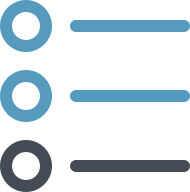
\includegraphics{images/_icons/alltutorials.png}}
\end{minipage}
\hfill
\begin{minipage}{0.90\textwidth}
%\vspace{-2mm}
\setlength{\parskip}{1em}
}{\end{minipage}
\end{mdframed}
%\vspace{2mm}
}

% singlelab

\newenvironment{singlelab}{
\vspace{2mm}
\begin{mdframed}[topline=false, bottomline=false, rightline=false, leftline=false]
\begin{minipage}{0.10\textwidth}
{$\:$ \\ \setkeys{Gin}{width=2em,keepaspectratio}
\includegraphics{images/_icons/singlelab.png}}
\end{minipage}
\hfill
\begin{minipage}{0.90\textwidth}
%\vspace{-2mm}
\setlength{\parskip}{1em}
}{\end{minipage}
\end{mdframed}
\vspace{2mm}
}

% todo

\newenvironment{todo}{
\vspace{4mm}
\begin{mdframed}[%
    topline=true, bottomline=true, linecolor=oiY, linewidth=0.5pt,
    rightline=false, leftline=false,
    backgroundcolor=oiLY]
\begin{minipage}[t]{0.10\textwidth}
{$\:$ \\ \setkeys{Gin}{width=2em,keepaspectratio}
\includegraphics{images/_icons/to-do.png}}
\end{minipage}
\hfill
\begin{minipage}[t]{0.90\textwidth}
\vspace{-2mm}
\setlength{\parskip}{1em}
\noindent\textbf{\color{oiGray}\small\Helvetica{{\MakeUppercase{TO DO}}}} $\:$ \\ \\
}{\end{minipage}
\end{mdframed}
\vspace{4mm}
}

% underconstruction

\newenvironment{underconstruction}{
\vspace{4mm}
\begin{mdframed}[%
    topline=true, bottomline=true, linecolor=oiR, linewidth=0.5pt,
    rightline=false, leftline=false,
    backgroundcolor=oiLR]
\begin{minipage}[t]{0.10\textwidth}
{$\:$ \\ \setkeys{Gin}{width=2em,keepaspectratio}
\includegraphics{images/_icons/under-construction.png}}
\end{minipage}
\hfill
\begin{minipage}[t]{0.90\textwidth}
\vspace{-2mm}
\setlength{\parskip}{1em}
\noindent\textbf{\color{oiR}\small\Helvetica{{\MakeUppercase{Under construction}}}} $\:$ \\ \\
}{\end{minipage}
\end{mdframed}
\vspace{4mm}
}

% Cover image ------------------------------------------------------------------

\newenvironment{authorinfo}[1]
  {
  \begin{minipage}[c]{0.30\textwidth}
  {\setkeys{Gin}{width=12em,keepaspectratio}\includegraphics{#1}}
  \end{minipage} 
  \hfill
  \begin{minipage}[c]{0.60\textwidth}
  }
  {
  \end{minipage}
  }

% Part formatting --------------------------------------------------------------

\titleformat{\part}[display]
{\color{oiR}\titlerule[5pt]\vspace{3pt}\color{oiLR}\titlerule[2pt]\vspace{3pt}\color{oiB}\normalfont\Huge\bfseries\scshape\Helvetica}
{\color{oiB}PART \thepart}{2em}{#1 \\ \noindent \vspace{3pt}\color{oiR}\titlerule[5pt]}

% https://tex.stackexchange.com/questions/506428/background-color-for-section-title
%\titleformat{\part}{\LARGE}{\rlap{\color{oiLB}\rule[-0.4cm]{\linewidth}{5cm}}\color{oiB}\normalfont\Huge\bfseries\scshape\Helvetica PART \thepart}{1em}{\color{oiB}\normalfont\Huge\bfseries\scshape\Helvetica #1}


% Bibliography: Chapter should be called References ----------------------------

%\usepackage{natbib}
%\usepackage{bibentry}
%\makeatletter\let\saved@bibitem\@bibitem\makeatother
%\usepackage{hyperref}
%\makeatletter\let\@bibitem\saved@bibitem\makeatother

% Index

\usepackage{makeidx}
\makeindex

% Smaller captions with bold labels

\usepackage[font=small,labelfont=bf]{caption}

% End ims-style.tex ------------------------------------------------------------
\usepackage{booktabs}
\usepackage{longtable}
\usepackage{array}
\usepackage{multirow}
\usepackage{wrapfig}
\usepackage{float}
\usepackage{colortbl}
\usepackage{pdflscape}
\usepackage{tabu}
\usepackage{threeparttable}
\usepackage{threeparttablex}
\usepackage[normalem]{ulem}
\usepackage{makecell}
\usepackage{xcolor}
\makeatletter
\@ifpackageloaded{bookmark}{}{\usepackage{bookmark}}
\makeatother
\makeatletter
\@ifpackageloaded{caption}{}{\usepackage{caption}}
\AtBeginDocument{%
\ifdefined\contentsname
  \renewcommand*\contentsname{Table of contents}
\else
  \newcommand\contentsname{Table of contents}
\fi
\ifdefined\listfigurename
  \renewcommand*\listfigurename{List of Figures}
\else
  \newcommand\listfigurename{List of Figures}
\fi
\ifdefined\listtablename
  \renewcommand*\listtablename{List of Tables}
\else
  \newcommand\listtablename{List of Tables}
\fi
\ifdefined\figurename
  \renewcommand*\figurename{Figure}
\else
  \newcommand\figurename{Figure}
\fi
\ifdefined\tablename
  \renewcommand*\tablename{Table}
\else
  \newcommand\tablename{Table}
\fi
}
\@ifpackageloaded{float}{}{\usepackage{float}}
\floatstyle{ruled}
\@ifundefined{c@chapter}{\newfloat{codelisting}{h}{lop}}{\newfloat{codelisting}{h}{lop}[chapter]}
\floatname{codelisting}{Listing}
\newcommand*\listoflistings{\listof{codelisting}{List of Listings}}
\makeatother
\makeatletter
\makeatother
\makeatletter
\@ifpackageloaded{caption}{}{\usepackage{caption}}
\@ifpackageloaded{subcaption}{}{\usepackage{subcaption}}
\makeatother
\ifLuaTeX
  \usepackage{selnolig}  % disable illegal ligatures
\fi
\usepackage{bookmark}

\IfFileExists{xurl.sty}{\usepackage{xurl}}{} % add URL line breaks if available
\urlstyle{same} % disable monospaced font for URLs
\hypersetup{
  pdftitle={Introduction to Modern Statistics (2e)},
  hidelinks,
  pdfcreator={LaTeX via pandoc}}

\title{Introduction to Modern Statistics (2e)}
\author{}
\date{}

\begin{document}
\frontmatter
\maketitle

\renewcommand*\contentsname{Table of contents}
{
\setcounter{tocdepth}{2}
\tableofcontents
}
\mainmatter
\bookmarksetup{startatroot}

\chapter*{Welcome to IMS2}\label{welcome-to-ims2}

\markboth{Welcome to IMS2}{Welcome to IMS2}

\chapter*{}

\vfill

Copyright \(\copyright\) 2024.

Second Edition.

Version date: April 29, 2024.

This textbook and its supplements, including slides, labs, and
interactive tutorials, may be downloaded for free at\\
\href{http://openintro.org/book/ims}{\textbf{openintro.org/book/ims}}.

This textbook is a derivative of \emph{OpenIntro Statistics} 4th Edition
and \emph{Introduction to Statistics with Randomization and Simulation}
1st Edition by Diez, Barr, and Çetinkaya-Rundel, and it's available
under a Creative Commons Attribution-ShareAlike 3.0 Unported United
States License. License details are available at the Creative Commons
website:\\
\href{https://www.openintro.org/go/?id=creativecommons_org&referrer=ims1_pdf}{\textbf{creativecommons.org}}.

Source files for this book can be found on GitHub at\\
\href{https://github.com/openintrostat/ims}{github.com/openintrostat/ims}.

\bookmarksetup{startatroot}

\chapter*{Authors}\label{authors}

\markboth{Authors}{Authors}

\vspace{-5mm}

\begin{authorinfo}{images/authors/mine.png}

\href{http://mine-cr.com/}{Mine Çetinkaya-Rundel}\\

Duke University, Posit, PBC.\\
\href{mailto:mine@openintro.org}{\nolinkurl{mine@openintro.org}}

\end{authorinfo}

Mine Çetinkaya-Rundel is Professor of the Practice at the Department of
Statistical Science at Duke University and Developer Educator at Posit.
Mine's work focuses on innovation in statistics and data science
pedagogy, with an emphasis on computing, reproducible research,
student-centered learning, and open-source education as well as
pedagogical approaches for enhancing retention of women and
under-represented minorities in STEM. Mine works on integrating
computation into the undergraduate statistics curriculum, using
reproducible research methodologies and analysis of real and complex
datasets. She also organizes
\href{https://ww2.amstat.org/education/datafest/}{ASA DataFest}, an
annual two-day competition in which teams of undergraduate students work
to reveal insights into a rich and complex dataset. Mine has been
working on the \href{https://www.openintro.org/}{OpenIntro} project
since its founding and as part of this project she co-authored four
open-source introductory statistics textbooks (including this one!). She
is also the creator and maintainer of
\href{https://datasciencebox.org/}{datasciencebox.org} and she teaches
the popular Statistics with R MOOC on Coursera. \newline

\begin{authorinfo}{images/authors/jo.png}

\href{https://research.pomona.edu/johardin/}{Johanna Hardin}\\

Pomona College\\
\href{mailto:jo.hardin@pomona.edu}{\nolinkurl{jo.hardin@pomona.edu}}

\end{authorinfo}

Jo Hardin is Professor of Mathematics and Statistics at Pomona College.
She collaborates with molecular biologists to create novel statistical
methods for analyzing high throughput data. She has also worked
extensively in statistics and data science education, facilitating
modern curricula for higher education instructors. She was a co-author
on the
\href{https://www.amstat.org/asa/education/Curriculum-Guidelines-for-Undergraduate-Programs-in-Statistical-Science.aspx}{2014
ASA Curriculum Guidelines for Undergraduate Programs in Statistical
Science}, and she writes on the blog
\href{https://teachdatascience.com/}{teachdatascience.com}. The best
part of her job is collaborating with undergraduate students. In her
spare time, she loves running, hiking, and jigsaw puzzles.

\bookmarksetup{startatroot}

\chapter*{Preface}\label{preface}
\addcontentsline{toc}{chapter}{Preface}

\markboth{Preface}{Preface}

\vspace{-10mm}

Welcome to the second edition of ``Introduction to Modern Statistics''!

We hope readers will take away three ideas from this book in addition to
forming a foundation of statistical thinking and methods.

\begin{enumerate}
\def\labelenumi{\arabic{enumi}.}
\tightlist
\item
  Statistics is an applied field with a wide range of practical
  applications.
\item
  You don't have to be a math guru to learn from interesting, real data.
\item
  Data are messy, and statistical tools are imperfect. However, when you
  understand the strengths and weaknesses of these tools, you can use
  them to learn interesting things about the world.
\end{enumerate}

\vspace{-2mm}

\section*{Textbook overview}\label{textbook-overview}

\markright{Textbook overview}

\begin{itemize}
\tightlist
\item
  \textbf{Part 1: Introduction to data.} Data structures, variables,
  summaries, graphics, and basic data collection and study design
  techniques.
\item
  \textbf{Part 2: Exploratory data analysis.} Data visualization and
  summarization, with particular emphasis on multivariable
  relationships.
\item
  \textbf{Part 3: Regression modeling.} Modeling numerical and
  categorical outcomes with linear and logistic regression and using
  model results to describe relationships and make predictions.
\item
  \textbf{Part 4: Foundations for inference.} Case studies are used to
  introduce the ideas of statistical inference with randomization tests,
  bootstrap intervals, and mathematical models.
\item
  \textbf{Part 5: Statistical inference.} Further details of statistical
  inference using randomization tests, bootstrap intervals, and
  mathematical models for numerical and categorical data.
\item
  \textbf{Part 6: Inferential modeling.} Extending inference techniques
  presented thus-far to linear and logistic regression settings and
  evaluating model performance.
\end{itemize}

Each part contains multiple chapters and ends with a case study.
Building on the content covered in the part, the case study presents a
high-level overview using the tools and techniques from the part.

In the chapters that cover statistical inference, we have presented a
parallel structure that walks the student through both computational and
mathematical approaches to every inferential topic. Trying to cover
every approach for every topic is likely too much material for a one
semester class. We suggest that you make deliberate choices for
navigating the book with your students. A few potential paths through
the book (with chapter numbers in parentheses) are given as follows:

\begin{itemize}
\tightlist
\item
  Focus on \textbf{parallel structure of computational and mathematical
  methods}: Introduction to data (1, 2), Exploratory data analysis (4,
  5), Regression (7), Foundations (11, 12, 13, 14), Inference (a subset
  of: 16, 17, 18, 19, 20, 21, 22; potentially: 16, 17, 19, 20).
\item
  Focus on \textbf{computational methods}: Introduction to data (1, 2),
  Exploratory data analysis (4, 5), Regression (7), Foundations (11, 12,
  14), Inference (computational methods only for some subset of: 16, 17,
  18, 19, 20, 21, 22).
\item
  Focus on \textbf{mathematical methods}: Introduction to data (1, 2),
  Exploratory data analysis (4, 5), Regression (7), Foundations (11, 12,
  13, 14), Inference (mathematical methods only for some subset of: 16,
  17, 18, 19, 20, 21, 22).
\item
  Focus on \textbf{modeling}: Introduction to data (1, 2), Exploratory
  data analysis (4, 5), Regression (7, 8, 9), Foundations (11, 12, 13,
  14), Inference (19), Inferential modeling (24, 25, 26).
\end{itemize}

We expect that most courses following a classical syllabus will not have
time to cover the chapters in the last part, Inferential modeling (24,
25, 26).

Each chapter ends with a review which contains a chapter summary as well
as a list of key terms introduced in the chapter. If you're not sure
what some of these terms mean, we recommend you go back in the text and
review their definitions. We purposefully present them in alphabetical
order, instead of in order of appearance, so they will be a little more
challenging to locate. However, you should be able to easily spot them
as \textbf{bolded text}.

\vspace{-2mm}

\section*{Changes for the second
edition}\label{changes-for-the-second-edition}

\markright{Changes for the second edition}

While the second edition does not represent a major change from the
first edition, we have worked hard to improve content, to add exercises,
and to update text and code to reflect changes in best practices (e.g.,
the book is now written in \href{https://quarto.org/}{Quarto}).

A brief summary of the biggest changes follows:

\begin{itemize}
\item
  Twenty-five completely new exercises were added. Most of the new
  exercises are concatenated onto existing exercises so as to retain
  similar numbering across editions. However, a few exercises have been
  moved in order to produce both odd exercises (with solutions) and even
  exercises (without solutions) on the same topic.
\item
  Multiple datasets were added or updated. For example, the
  \href{http://openintrostat.github.io/openintro/reference/pm25_2022_durham.html}{\texttt{pm25\_2022\_durham}}
  data on air quality in Durham, NC in 2022 can be found in the
  \href{https://openintrostat.github.io/openintro/}{\textbf{openintro}}
  R package.
\item
  Chapter~\ref{sec-data-applications} was re-written with an updated
  context and data example. Additionally, in
  Chapter~\ref{sec-data-applications}, we explore Simpson's Paradox.
\item
  Throughout the text and the exercises, ``statistically significant''
  has been changed to ``statistically discernible'' so as to distance
  ourselves from the more colloquial use of the word ``significant.''
\end{itemize}

\vspace{-2mm}

\section*{Examples and exercises}\label{examples-and-exercises}

\markright{Examples and exercises}

Examples are provided to establish an understanding of how to apply
methods.

\begin{workedexample}
This is an example. When a question is asked here, where can the answer
be found?

\begin{center}\rule{0.5\linewidth}{0.5pt}\end{center}

The answer can be found here, in the solution section of the example!

\end{workedexample}

When we think the reader is ready to try determining a solution on their
own, we frame it as Guided Practice.

\begin{guidedpractice}
The reader may check or learn the answer to any Guided Practice problem
by reviewing the full solution in a footnote.\footnote{Guided Practice
  problems are intended to stretch your thinking, and you can check
  yourself by reviewing the footnote solution for any Guided Practice.}

\end{guidedpractice}

Exercises are also provided at the end of each chapter. Solutions are
given for odd-numbered exercises in
Appendix~\ref{sec-exercise-solutions}.

\vspace{-2mm}

\section*{Datasets and their sources}\label{datasets-and-their-sources}

\markright{Datasets and their sources}

A large majority of the datasets used in the book can be found in
various R packages. Each time a new dataset is introduced in the
narrative, a reference to the package like the one below is provided.
Many of these datasets are in the
\href{http://openintrostat.github.io/openintro}{\textbf{openintro}} R
package that contains datasets used in
\href{https://www.openintro.org/}{OpenIntro}'s open-source
textbooks.\footnote{Mine Çetinkaya-Rundel and David Diez and Andrew Bray
  and Albert Y. Kim and Ben Baumer and Chester Ismay and Nick Paterno
  and Christopher Barr (2024). openintro: Data Sets and Supplemental
  Functions from `OpenIntro' Textbooks and Labs. R package version
  2.4.0. \url{https://github.com/openintrostat/openintro}.}

\begin{data}
The
\href{http://openintrostat.github.io/openintro/reference/textbooks.html}{\texttt{textbooks}}
data can be found in the
\href{http://openintrostat.github.io/openintro}{\textbf{openintro}} R
package.

\end{data}

The datasets used throughout the book come from real sources like
opinion polls and scientific articles, except for a handful of cases
where we use toy data to highlight a particular feature or explain a
particular concept. References for the sources of the real data are
provided at the end of the book.

\vspace{-2mm}

\section*{Computing with R}\label{computing-with-r}

\markright{Computing with R}

The narrative and the exercises in the book are computing language
agnostic, however while it's possible to learn about modern statistics
without computing, it's not possible to apply it. Therefore, we invite
you to navigate the concepts you have learned in each part using the
interactive R tutorials and the R labs that are included at the end of
each part.

\vspace{-2mm}

\subsection*{Interactive R tutorials}\label{interactive-r-tutorials}

The self-paced and interactive R tutorials were developed using the
\href{https://rstudio.github.io/learnr/index.html}{learnr} R package,
and only an internet browser is needed to complete them.

\begin{alltutorials}
Each part comes with a tutorial comprised of 4-10 lessons and listed
like this.

\end{alltutorials}

\begin{singletutorial}
Each of these lessons is listed like this.

\end{singletutorial}

You can access the full list of tutorials supporting this book
\url{https://openintrostat.github.io/ims-tutorials}.

\vspace{-2mm}

\subsection*{R labs}\label{r-labs}

Once you feel comfortable with the material in the tutorials, we also
encourage you to apply what you've learned via the computational labs
that are also linked at the end of each part. The labs consist of data
analysis case studies, and they require access to
\href{https://cran.r-project.org/}{R} and
\href{https://posit.co/products/open-source/rstudio/}{RStudio}. The
first lab includes installation instructions. If you'd rather not
install the software locally, you can also try
\href{https://posit.cloud/}{Posit Cloud} for free.

\begin{singlelab}
Labs for each part are listed like this.

\end{singlelab}

You can access the full list of labs supporting this book at\\
\href{https://www.openintro.org/go?id=ims-r-labs}{openintro.org/go?id=ims-r-labs}.

\vspace{-2mm}

\section*{OpenIntro, online resources, and getting
involved}\label{openintro-online-resources-and-getting-involved}

\markright{OpenIntro, online resources, and getting involved}

OpenIntro is an organization focused on developing free and affordable
education materials. We encourage anyone learning or teaching statistics
to visit \href{http://www.openintro.org}{openintro.org} and to get
involved.

All OpenIntro resources are free and anyone is welcomed to use these
online tools and resources with or without this textbook as a companion.

We value your feedback. If there is a part of the project you especially
like or think needs improvement, we want to hear from you. For feedback
on this specific book, you can open an issue on the GitHub repository of
the book at
\href{https://github.com/openintrostat/ims}{github.com/openintrostat/ims}.
You can also provide feedback on this book or any other OpenIntro
resource via our contact form at
\href{https://www.openintro.org/form/?f=contact}{openintro.org}.

\vspace{-2mm}

\section*{Acknowledgements}\label{acknowledgements}

\markright{Acknowledgements}

The \emph{OpenIntro} project would not have been possible without the
dedication and volunteer hours of all those involved, and we hope you
will join us in extending a huge \emph{thank you} to all those who
volunteer with OpenIntro.

The authors would like to thank the following individuals:

\begin{itemize}
\tightlist
\item
  David Diez and Christopher Barr for their work on the 1st Edition of
  this book,
\item
  Ben Baumer and Andrew Bray for their contribution rethinking how and
  which order we present this material as well as their work as original
  authors of the interactive tutorial content,
\item
  Yanina Bellini Saibene, Florencia D'Andrea, and Roxana Noelia
  Villafañe for their work on creating the interactive tutorials in
  learnr,
\item
  Peter Baumgartner for review and revisions of the interactive learnr
  tutorials,
\item
  Will Gray for conceptual diagrams,
\item
  Allison Theobold, Melinda Yager, and Randy Prium for their valuable
  feedback and review of the book,
\item
  Colin Rundel for feedback on content and technical help with
  conversion from LaTeX to R Markdown,
\item
  Christophe Dervieux for help with multi-output bookdown issues, and
\item
  Müge Çetinkaya and Meenal Patel for their design vision.
\end{itemize}

We would like to also thank the developers of the open-source tools that
make the development and authoring of this book possible, e.g.,
\href{https://quarto.org/}{Quarto},
\href{https://tidyverse.org/}{tidyverse},
\href{https://tidymodels.org/}{tidymodels}, and
\href{http://icons8.com/}{icons8}.

We are also grateful to the many teachers, students, and other readers
who have helped improve OpenIntro resources through their feedback.

\part{Introduction to data}

The first part of the book will introduce you to data, their properties,
how they are collected, and the structure of the design used for the
study. Different data and settings lead to different \textbf{types} of
conclusions, so you'll always want to keep in mind the data provenance,
especially as you move on to modeling and inference.

\begin{itemize}
\item
  In Chapter~\ref{sec-data-hello} you'll be introduced to tidy data, an
  important structure for describing, visualizing, and analyzing data.
\item
  In Chapter~\ref{sec-data-design} the focus is on study design. In
  particular, the critical distinction between random sampling and
  randomization is made.
\item
  Chapter~\ref{sec-data-applications} includes an application on the
  Paralympics case study where the topics from the Introduction to data
  part of the book are fully developed.
\end{itemize}

We recommend you come back to review this foundational part after you
cover each new part in the textbook. In particular, it is worthwhile to
consider Figure~\ref{fig-randsampValloc} in all of the inferential
settings you cover. Each dataset you analyze will have a slightly
different context which will require thoughtful consideration of the
appropriate conclusions.

\chapter{Hello data}\label{sec-data-hello}

\begin{chapterintro}
Scientists seek to answer questions using rigorous methods and careful
observations. These observations -- collected from the likes of field
notes, surveys, and experiments -- form the backbone of a statistical
investigation and are called \textbf{data}. Statistics is the study of
how best to collect, analyze, and draw conclusions from data. In this
first chapter, we focus on both the properties of data and on the
collection of data.

\end{chapterintro}

\section{Case study: Using stents to prevent
strokes}\label{sec-case-study-stents-strokes}

In this section we introduce a classic challenge in statistics:
evaluating the efficacy of a medical treatment. Terms in this section,
and indeed much of this chapter, will all be revisited later in the
text. The plan for now is simply to get a sense of the role statistics
can play in practice.

An experiment is designed to study the effectiveness of stents in
treating patients at risk of stroke (Chimowitz et al. 2011). Stents are
small mesh tubes that are placed inside narrow or weak arteries to
assist in patient recovery after cardiac events and reduce the risk of
an additional heart attack or death.

Many doctors have hoped that there would be similar benefits for
patients at risk of stroke. We start by writing the principal question
the researchers hope to answer:

\begin{quote}
Does the use of stents reduce the risk of stroke?
\end{quote}

The researchers who asked this question conducted an experiment with 451
at-risk patients. Each volunteer patient was randomly assigned to one of
two groups:

\begin{itemize}
\tightlist
\item
  \textbf{Treatment group}. Patients in the treatment group received a
  stent and medical management. The medical management included
  medications, management of risk factors, and help in lifestyle
  modification.
\item
  \textbf{Control group}. Patients in the control group received the
  same medical management as the treatment group, but they did not
  receive stents.
\end{itemize}

Researchers randomly assigned 224 patients to the treatment group and
227 to the control group. In this study, the control group provides a
reference point against which we can measure the medical impact of
stents in the treatment group.

Researchers studied the effect of stents at two time points: 30 days
after enrollment and 365 days after enrollment. The results of 5
patients are summarized in Table~\ref{tbl-stentStudyResultsDF}. Patient
outcomes are recorded as \texttt{stroke} or \texttt{no\ event},
representing whether the patient had a stroke during that time period.

\begin{data}
The
\href{http://openintrostat.github.io/openintro/reference/stent30.html}{\texttt{stent30}}
data and
\href{http://openintrostat.github.io/openintro/reference/stent365.html}{\texttt{stent365}}
data can be found in the
\href{http://openintrostat.github.io/openintro}{\textbf{openintro}} R
package.

\end{data}

\begin{table}

\caption{\label{tbl-stentStudyResultsDF}Results for five patients from
the stent study.}

\centering{

\centering
\begin{tabular}[t]{>{\raggedright\arraybackslash}p{8em}>{\raggedright\arraybackslash}p{8em}>{\raggedright\arraybackslash}p{8em}>{\raggedright\arraybackslash}p{8em}}
\toprule
patient & group & 30 days & 365 days\\
\midrule
\cellcolor{gray!10}{1} & \cellcolor{gray!10}{treatment} & \cellcolor{gray!10}{no event} & \cellcolor{gray!10}{no event}\\
2 & treatment & stroke & stroke\\
\cellcolor{gray!10}{3} & \cellcolor{gray!10}{treatment} & \cellcolor{gray!10}{no event} & \cellcolor{gray!10}{no event}\\
4 & treatment & no event & no event\\
\cellcolor{gray!10}{5} & \cellcolor{gray!10}{control} & \cellcolor{gray!10}{no event} & \cellcolor{gray!10}{no event}\\
\bottomrule
\end{tabular}

}

\end{table}%

It would be difficult to answer a question on the impact of stents on
the occurrence of strokes for \textbf{all} study patients using these
\emph{individual} observations. This question is better addressed by
performing a statistical data analysis of \emph{all} observations.
Table~\ref{tbl-stentStudyResultsDFsummary} summarizes the raw data in a
more helpful way. In this table, we can quickly see what happened over
the entire study. For instance, to identify the number of patients in
the treatment group who had a stroke within 30 days after the treatment,
we look in the leftmost column (30 days), at the intersection of
treatment and stroke: 33. To identify the number of control patients who
did not have a stroke after 365 days after receiving treatment, we look
at the rightmost column (365 days), at the intersection of control and
no event: 199.

\begin{table}

\caption{\label{tbl-stentStudyResultsDFsummary}Descriptive statistics
for the stent study.}

\centering{

\centering
\begin{tabular}[t]{lrrrr}
\toprule
\multicolumn{1}{c}{ } & \multicolumn{2}{c}{30 days} & \multicolumn{2}{c}{365 days} \\
\cmidrule(l{3pt}r{3pt}){2-3} \cmidrule(l{3pt}r{3pt}){4-5}
Group & Stroke & No event & Stroke & No event\\
\midrule
\cellcolor{gray!10}{Control} & \cellcolor{gray!10}{13} & \cellcolor{gray!10}{214} & \cellcolor{gray!10}{28} & \cellcolor{gray!10}{199}\\
Treatment & 33 & 191 & 45 & 179\\
\cellcolor{gray!10}{Total} & \cellcolor{gray!10}{46} & \cellcolor{gray!10}{405} & \cellcolor{gray!10}{73} & \cellcolor{gray!10}{378}\\
\bottomrule
\end{tabular}

}

\end{table}%

\begin{guidedpractice}
Of the 224 patients in the treatment group, 45 had a stroke by the end
of the first year. Using these two numbers, compute the proportion of
patients in the treatment group who had a stroke by the end of their
first year. (Note: answers to all Guided Practice exercises are provided
in footnotes!)\footnote{The proportion of the 224 patients who had a
  stroke within 365 days: \(45/224 = 0.20.\)}

\end{guidedpractice}

We can compute summary statistics from the table to give us a better
idea of how the impact of the stent treatment differed between the two
groups. A \textbf{summary statistic} is a single number summarizing data
from a sample.\index{summary statistic} For instance, the primary
results of the study after 1 year could be described by two summary
statistics: the proportion of people who had a stroke in the treatment
and control groups.

\begin{itemize}
\tightlist
\item
  Proportion who had a stroke in the treatment (stent) group:
  \(45/224 = 0.20 = 20\%.\)
\item
  Proportion who had a stroke in the control group:
  \(28/227 = 0.12 = 12\%.\)
\end{itemize}

These two summary statistics are useful in looking for differences in
the groups, and we are in for a surprise: an additional 8\% of patients
in the treatment group had a stroke! This is important for two reasons.
First, it is contrary to what doctors expected, which was that stents
would \emph{reduce} the rate of strokes. Second, it leads to a
statistical question: do the data show a ``real'' difference between the
groups?

This second question is subtle. Suppose you flip a coin 100 times. While
the chance a coin lands heads in any given coin flip is 50\%, we
probably won't observe exactly 50 heads. This type of variation is part
of almost any type of data generating process. It is possible that the
8\% difference in the stent study is due to this natural variation.
However, the larger the difference we observe (for a particular sample
size), the less believable it is that the difference is due to chance.
So, what we are really asking is the following: if in fact stents have
no effect, how likely is it that we observe such a large difference?

While we do not yet have statistical tools to fully address this
question on our own, we can comprehend the conclusions of the published
analysis: there was compelling evidence of harm by stents in this study
of stroke patients.

\textbf{Be careful:} Do not generalize the results of this study to all
patients and all stents. This study looked at patients with very
specific characteristics who volunteered to be a part of this study and
who may not be representative of all stroke patients. In addition, there
are many types of stents, and this study only considered the
self-expanding Wingspan stent (Boston Scientific). However, this study
does leave us with an important lesson: we should keep our eyes open for
surprises.

\section{Data basics}\label{sec-data-basics}

Effective presentation and description of data is a first step in most
analyses. This section introduces one structure for organizing data as
well as some terminology that will be used throughout this book.

\subsection{Observations, variables, and data
matrices}\label{observations-variables-and-data-matrices}

Table~\ref{tbl-loan50-df} displays six rows of a dataset for 50 randomly
sampled loans offered through Lending Club, which is a peer-to-peer
lending company. This dataset will be referred to as \texttt{loan50}.

\begin{data}
The
\href{http://openintrostat.github.io/openintro/reference/loans_full_schema.html}{\texttt{loan50}}
data can be found in the
\href{http://openintrostat.github.io/openintro}{\textbf{openintro}} R
package.

\end{data}

Each row in the table represents a single loan. The formal name for a
row is a \index{case}\textbf{case} or
\index{observation}\textbf{observation} or
\index{unit of observation}\textbf{unit of observation}. The columns
represent characteristics of each loan, where each column is referred to
as a \index{variable}\textbf{variable}. For example, the first row
represents a loan of \$22,000 with an interest rate of 10.90\%, where
the borrower is based in New Jersey (NJ) and has an income of \$59,000.

\begin{guidedpractice}
What is the grade of the first loan in Table~\ref{tbl-loan50-df}? And
what is the home ownership status of the borrower for that first loan?
Reminder: for these Guided Practice questions, you can check your answer
in the footnote.\footnote{The loan's grade is B, and the borrower rents
  their residence.}

\end{guidedpractice}

In practice, it is especially important to ask clarifying questions to
ensure important aspects of the data are understood. For instance, it is
always important to be sure we know what each variable means and its
units of measurement. Descriptions of the variables in the
\texttt{loan50} dataset are given in Table~\ref{tbl-loan-50-variables}.

\begin{table}

\caption{\label{tbl-loan50-df}Six observations from the \texttt{loan50}
dataset.}

\centering{

\centering
\begin{tabular}[t]{lrrrllrl}
\toprule
  & loan\_amount & interest\_rate & term & grade & state & total\_income & homeownership\\
\midrule
\cellcolor{gray!10}{1} & \cellcolor{gray!10}{22,000} & \cellcolor{gray!10}{10.90} & \cellcolor{gray!10}{60} & \cellcolor{gray!10}{B} & \cellcolor{gray!10}{NJ} & \cellcolor{gray!10}{59,000} & \cellcolor{gray!10}{rent}\\
2 & 6,000 & 9.92 & 36 & B & CA & 60,000 & rent\\
\cellcolor{gray!10}{3} & \cellcolor{gray!10}{25,000} & \cellcolor{gray!10}{26.30} & \cellcolor{gray!10}{36} & \cellcolor{gray!10}{E} & \cellcolor{gray!10}{SC} & \cellcolor{gray!10}{75,000} & \cellcolor{gray!10}{mortgage}\\
4 & 6,000 & 9.92 & 36 & B & CA & 75,000 & rent\\
\cellcolor{gray!10}{5} & \cellcolor{gray!10}{25,000} & \cellcolor{gray!10}{9.43} & \cellcolor{gray!10}{60} & \cellcolor{gray!10}{B} & \cellcolor{gray!10}{OH} & \cellcolor{gray!10}{254,000} & \cellcolor{gray!10}{mortgage}\\
6 & 6,400 & 9.92 & 36 & B & IN & 67,000 & mortgage\\
\bottomrule
\end{tabular}

}

\end{table}%

\begin{table}

\caption{\label{tbl-loan-50-variables}Variables and their descriptions
for the \texttt{loan50} dataset.}

\centering{

\centering
\begin{tabular}[t]{>{}l>{\raggedright\arraybackslash}p{30em}}
\toprule
Variable & Description\\
\midrule
\ttfamily{\cellcolor{gray!10}{loan\_amount}} & \cellcolor{gray!10}{Amount of the loan received, in US dollars.}\\
\ttfamily{interest\_rate} & Interest rate on the loan, in an annual percentage.\\
\ttfamily{\cellcolor{gray!10}{term}} & \cellcolor{gray!10}{The length of the loan, which is always set as a whole number of months.}\\
\ttfamily{grade} & Loan grade, which takes a values A through G and represents the quality of the loan and its likelihood of being repaid.\\
\ttfamily{\cellcolor{gray!10}{state}} & \cellcolor{gray!10}{US state where the borrower resides.}\\
\ttfamily{total\_income} & Borrower's total income, including any second income, in US dollars.\\
\ttfamily{\cellcolor{gray!10}{homeownership}} & \cellcolor{gray!10}{Indicates whether the person owns, owns but has a mortgage, or rents.}\\
\bottomrule
\end{tabular}

}

\end{table}%

The data in Table~\ref{tbl-loan50-df} represent a
\index{data frame}\textbf{data frame}, which is a convenient and common
way to organize data, especially if collecting data in a spreadsheet. A
data frame where each row is a unique case (observational unit), each
column is a variable, and each cell is a single value is commonly
referred to as \index{tidy data}\textbf{tidy data} (Wickham 2014).

When recording data, use a tidy data frame unless you have a very good
reason to use a different structure. This structure allows new cases to
be added as rows or new variables as new columns and facilitates
visualization, summarization, and other statistical analyses.

\begin{guidedpractice}
The grades for assignments, quizzes, and exams in a course are often
recorded in a gradebook that takes the form of a data frame. How might
you organize a course's grade data using a data frame? Describe the
observational units and variables.\footnote{There are multiple
  strategies that can be followed. One common strategy is to have each
  student represented by a row, and then add a column for each
  assignment, quiz, or exam. Under this setup, it is easy to review a
  single line to understand the grade history of a student. There should
  also be columns to include student information, such as one column to
  list student names.}

\end{guidedpractice}

\begin{guidedpractice}
We consider data for 3,142 counties in the United States, which includes
the name of each county, the state where it resides, its population in
2017, the population change from 2010 to 2017, poverty rate, and nine
additional characteristics. How might these data be organized in a data
frame?\footnote{Each county may be viewed as a case, and there are
  eleven pieces of information recorded for each case. A table with
  3,142 rows and 14 columns could hold these data, where each row
  represents a county and each column represents a particular piece of
  information.}

\end{guidedpractice}

The data described in the Guided Practice above represents the
\texttt{county} dataset, which is shown as a data frame in
Table~\ref{tbl-county-df}. The variables as well as the variables in the
dataset that did not fit in Table~\ref{tbl-county-df} are described in
Table~\ref{tbl-county-variables}.

\begin{table}

\caption{\label{tbl-county-df}Six observations and six variables from
the \texttt{county} dataset.}

\centering{

\centering
\begin{tabular}[t]{llrrrl}
\toprule
name & state & pop2017 & pop\_change & unemployment\_rate & median\_edu\\
\midrule
\cellcolor{gray!10}{Autauga County} & \cellcolor{gray!10}{Alabama} & \cellcolor{gray!10}{55,504} & \cellcolor{gray!10}{1.48} & \cellcolor{gray!10}{3.86} & \cellcolor{gray!10}{some\_college}\\
Baldwin County & Alabama & 212,628 & 9.19 & 3.99 & some\_college\\
\cellcolor{gray!10}{Barbour County} & \cellcolor{gray!10}{Alabama} & \cellcolor{gray!10}{25,270} & \cellcolor{gray!10}{-6.22} & \cellcolor{gray!10}{5.90} & \cellcolor{gray!10}{hs\_diploma}\\
Bibb County & Alabama & 22,668 & 0.73 & 4.39 & hs\_diploma\\
\cellcolor{gray!10}{Blount County} & \cellcolor{gray!10}{Alabama} & \cellcolor{gray!10}{58,013} & \cellcolor{gray!10}{0.68} & \cellcolor{gray!10}{4.02} & \cellcolor{gray!10}{hs\_diploma}\\
Bullock County & Alabama & 10,309 & -2.28 & 4.93 & hs\_diploma\\
\bottomrule
\end{tabular}

}

\end{table}%

\begin{table}

\caption{\label{tbl-county-variables}Variables and their descriptions
for the \texttt{county} dataset.}

\centering{

\centering
\begin{tabular}[t]{>{}l>{\raggedright\arraybackslash}p{30em}}
\toprule
Variable & Description\\
\midrule
\ttfamily{\cellcolor{gray!10}{name}} & \cellcolor{gray!10}{Name of county.}\\
\ttfamily{state} & Name of state.\\
\ttfamily{\cellcolor{gray!10}{pop2000}} & \cellcolor{gray!10}{Population in 2000.}\\
\ttfamily{pop2010} & Population in 2010.\\
\ttfamily{\cellcolor{gray!10}{pop2017}} & \cellcolor{gray!10}{Population in 2017.}\\
\ttfamily{pop\_change} & Population change from 2010 to 2017 (in percent).\\
\ttfamily{\cellcolor{gray!10}{poverty}} & \cellcolor{gray!10}{Percent of population in poverty in 2017.}\\
\ttfamily{homeownership} & Homeownership rate, 2006-2010.\\
\ttfamily{\cellcolor{gray!10}{multi\_unit}} & \cellcolor{gray!10}{Multi-unit rate: percent of housing units that are in multi-unit structures, 2006-2010.}\\
\ttfamily{unemployment\_rate} & Unemployment rate in 2017.\\
\ttfamily{\cellcolor{gray!10}{metro}} & \cellcolor{gray!10}{Whether the county contains a metropolitan area, taking one of the values yes or no.}\\
\ttfamily{median\_edu} & Median education level (2013-2017), taking one of the values below\_hs, hs\_diploma, some\_college, or bachelors.\\
\ttfamily{\cellcolor{gray!10}{per\_capita\_income}} & \cellcolor{gray!10}{Per capita (per person) income (2013-2017).}\\
\ttfamily{median\_hh\_income} & Median household income.\\
\ttfamily{\cellcolor{gray!10}{smoking\_ban}} & \cellcolor{gray!10}{Describes the type of county-level smoking ban in place in 2010, taking one of the values none, partial, or comprehensive.}\\
\bottomrule
\end{tabular}

}

\end{table}%

\begin{data}
The
\href{http://openintrostat.github.io/usdata/reference/county.html}{\texttt{county}}
data can be found in the
\href{http://openintrostat.github.io/usdata}{\textbf{usdata}} R package.

\end{data}

\subsection{Types of variables}\label{sec-variable-types}

Examine the \texttt{unemployment\_rate}, \texttt{pop2017},
\texttt{state}, and \texttt{median\_edu} variables in the
\texttt{county} dataset. Each of these variables is inherently different
from the other three, yet some share certain characteristics.

First consider \texttt{unemployment\_rate}, which is said to be a
\index{variable!numerical}\textbf{numerical} variable since it can take
a wide range of numerical values, and it is sensible to add, subtract,
or take averages with those values. On the other hand, we would not
classify a variable reporting telephone area codes as numerical since
the average, sum, and difference of area codes does not have any clear
meaning. Instead, we would consider area codes as a categorical
variable.

The \texttt{pop2017} variable is also numerical, although it seems to be
a little different than \texttt{unemployment\_rate}. This variable of
the population count can only take whole non-negative numbers (0, 1, 2,
\ldots). For this reason, the population variable is said to be
\textbf{discrete}\index{variable!discrete} since it can only take
numerical values with jumps. On the other hand, the unemployment rate
variable is said to be \textbf{continuous}\index{variable!continuous}.

The variable \texttt{state} can take up to 51 values after accounting
for Washington, DC: Alabama, Alaska, \ldots, and Wyoming. Because the
responses themselves are categories, \texttt{state} is called a
\textbf{categorical} variable, and the possible values (states) are
called the variable's \textbf{levels} (e.g., District of Columbia,
Alabama, Alaska, etc.) .

Finally, consider the \texttt{median\_edu} variable, which describes the
median education level of county residents and takes values
\texttt{below\_hs}, \texttt{hs\_diploma}, \texttt{some\_college}, or
\texttt{bachelors} in each county. This variable seems to be a hybrid:
it is a categorical variable, but the levels have a natural ordering. A
variable with these properties is called an
\textbf{ordinal}\index{variable!ordinal} variable, while a regular
categorical variable without this type of special ordering is called a
\textbf{nominal}\index{variable!nominal} variable. To simplify analyses,
any categorical variable in this book will be treated as a nominal
(unordered) categorical variable (see Figure~\ref{fig-variables}).

\begin{figure}[H]

\centering{

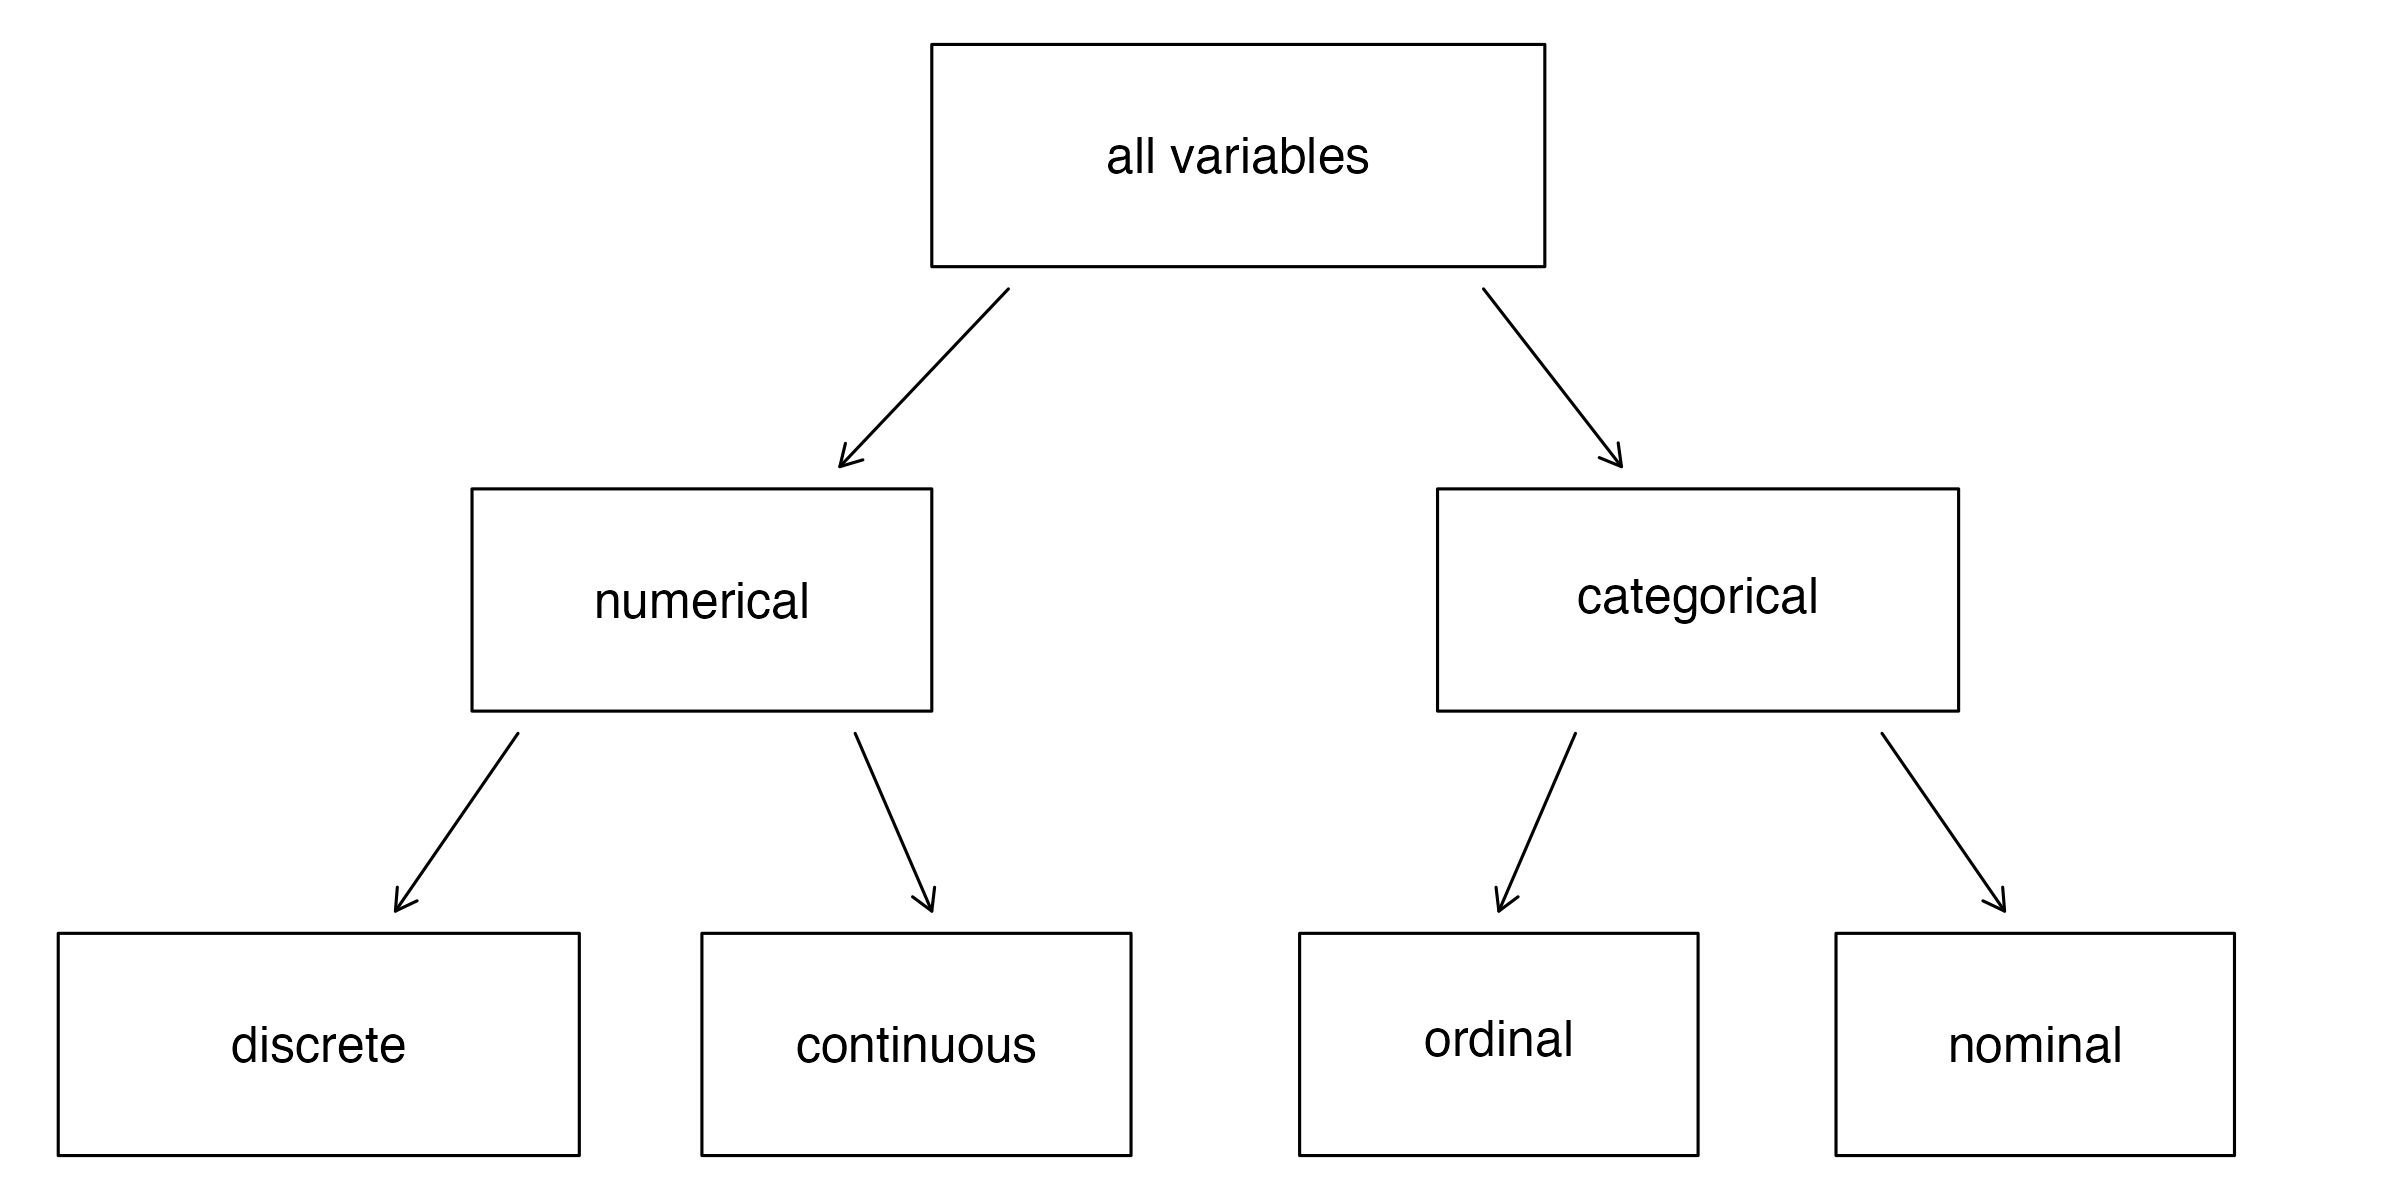
\includegraphics[width=0.7\textwidth,height=\textheight]{01-data-hello_files/figure-pdf/fig-variables-1.png}

}

\caption{\label{fig-variables}Breakdown of variables into their
respective types.}

\end{figure}%

\begin{workedexample}
Data were collected about students in a statistics course. Three
variables were recorded for each student: number of siblings, student
height, and whether the student had previously taken a statistics
course. Classify each of the variables as continuous numerical, discrete
numerical, or categorical.

\begin{center}\rule{0.5\linewidth}{0.5pt}\end{center}

The number of siblings and student height represent numerical variables.
Because the number of siblings is a count, it is discrete. Height varies
continuously, so it is a continuous numerical variable. The last
variable classifies students into two categories -- those who have and
those who have not taken a statistics course -- which makes this
variable categorical.

\end{workedexample}

\begin{guidedpractice}
An experiment is evaluating the effectiveness of a new drug in treating
migraines. A \texttt{group} variable is used to indicate the experiment
group for each patient: treatment or control. The
\texttt{num\_migraines} variable represents the number of migraines the
patient experienced during a 3-month period. Classify each variable as
either numerical or categorical?\footnote{The \texttt{group} variable
  can take just one of two group names, making it categorical. The
  \texttt{num\_migraines} variable describes a count of the number of
  migraines, which is an outcome where basic arithmetic is sensible,
  which means this is a numerical outcome; more specifically, since it
  represents a count, \texttt{num\_migraines} is a discrete numerical
  variable.}

\end{guidedpractice}

\subsection{Relationships between
variables}\label{sec-variable-relations}

Many analyses are motivated by a researcher looking for a relationship
between two or more variables. A social scientist may like to answer
some of the following questions:

\begin{quote}
Does a higher-than-average increase in county population tend to
correspond to counties with higher or lower median household incomes?
\end{quote}

\begin{quote}
If homeownership in one county is lower than the national average, will
the percent of housing units that are in multi-unit structures in that
county tend to be above or below the national average?
\end{quote}

\begin{quote}
How much can the median education level explain the median household
income for counties in the US?
\end{quote}

To answer these questions, data must be collected, such as the
\texttt{county} dataset shown in Table~\ref{tbl-county-df}. Examining
\index{summary statistic}\textbf{summary statistics} can provide
numerical insights about the specifics of each of these questions.
Alternatively, graphs can be used to visually explore the data,
potentially providing more insight than a summary statistic.

\index{scatterplot}\textbf{Scatterplots} are one type of graph used to
study the relationship between two numerical variables.
Figure~\ref{fig-county-multi-unit-homeownership} displays the
relationship between the variables \texttt{homeownership} and
\texttt{multi\_unit}, which is the percent of housing units that are in
multi-unit structures (e.g., apartments, condos). Each point on the plot
represents a single county. For instance, the highlighted dot
corresponds to County 413 in the \texttt{county} dataset: Chattahoochee
County, Georgia, which has 39.4\% of housing units that are in
multi-unit structures and a homeownership rate of 31.3\%. The
scatterplot suggests a relationship between the two variables: counties
with a higher rate of housing units that are in multi-unit structures
tend to have lower homeownership rates. We might brainstorm as to why
this relationship exists and investigate each idea to determine which
are the most reasonable explanations.

\begin{figure}[H]

\centering{

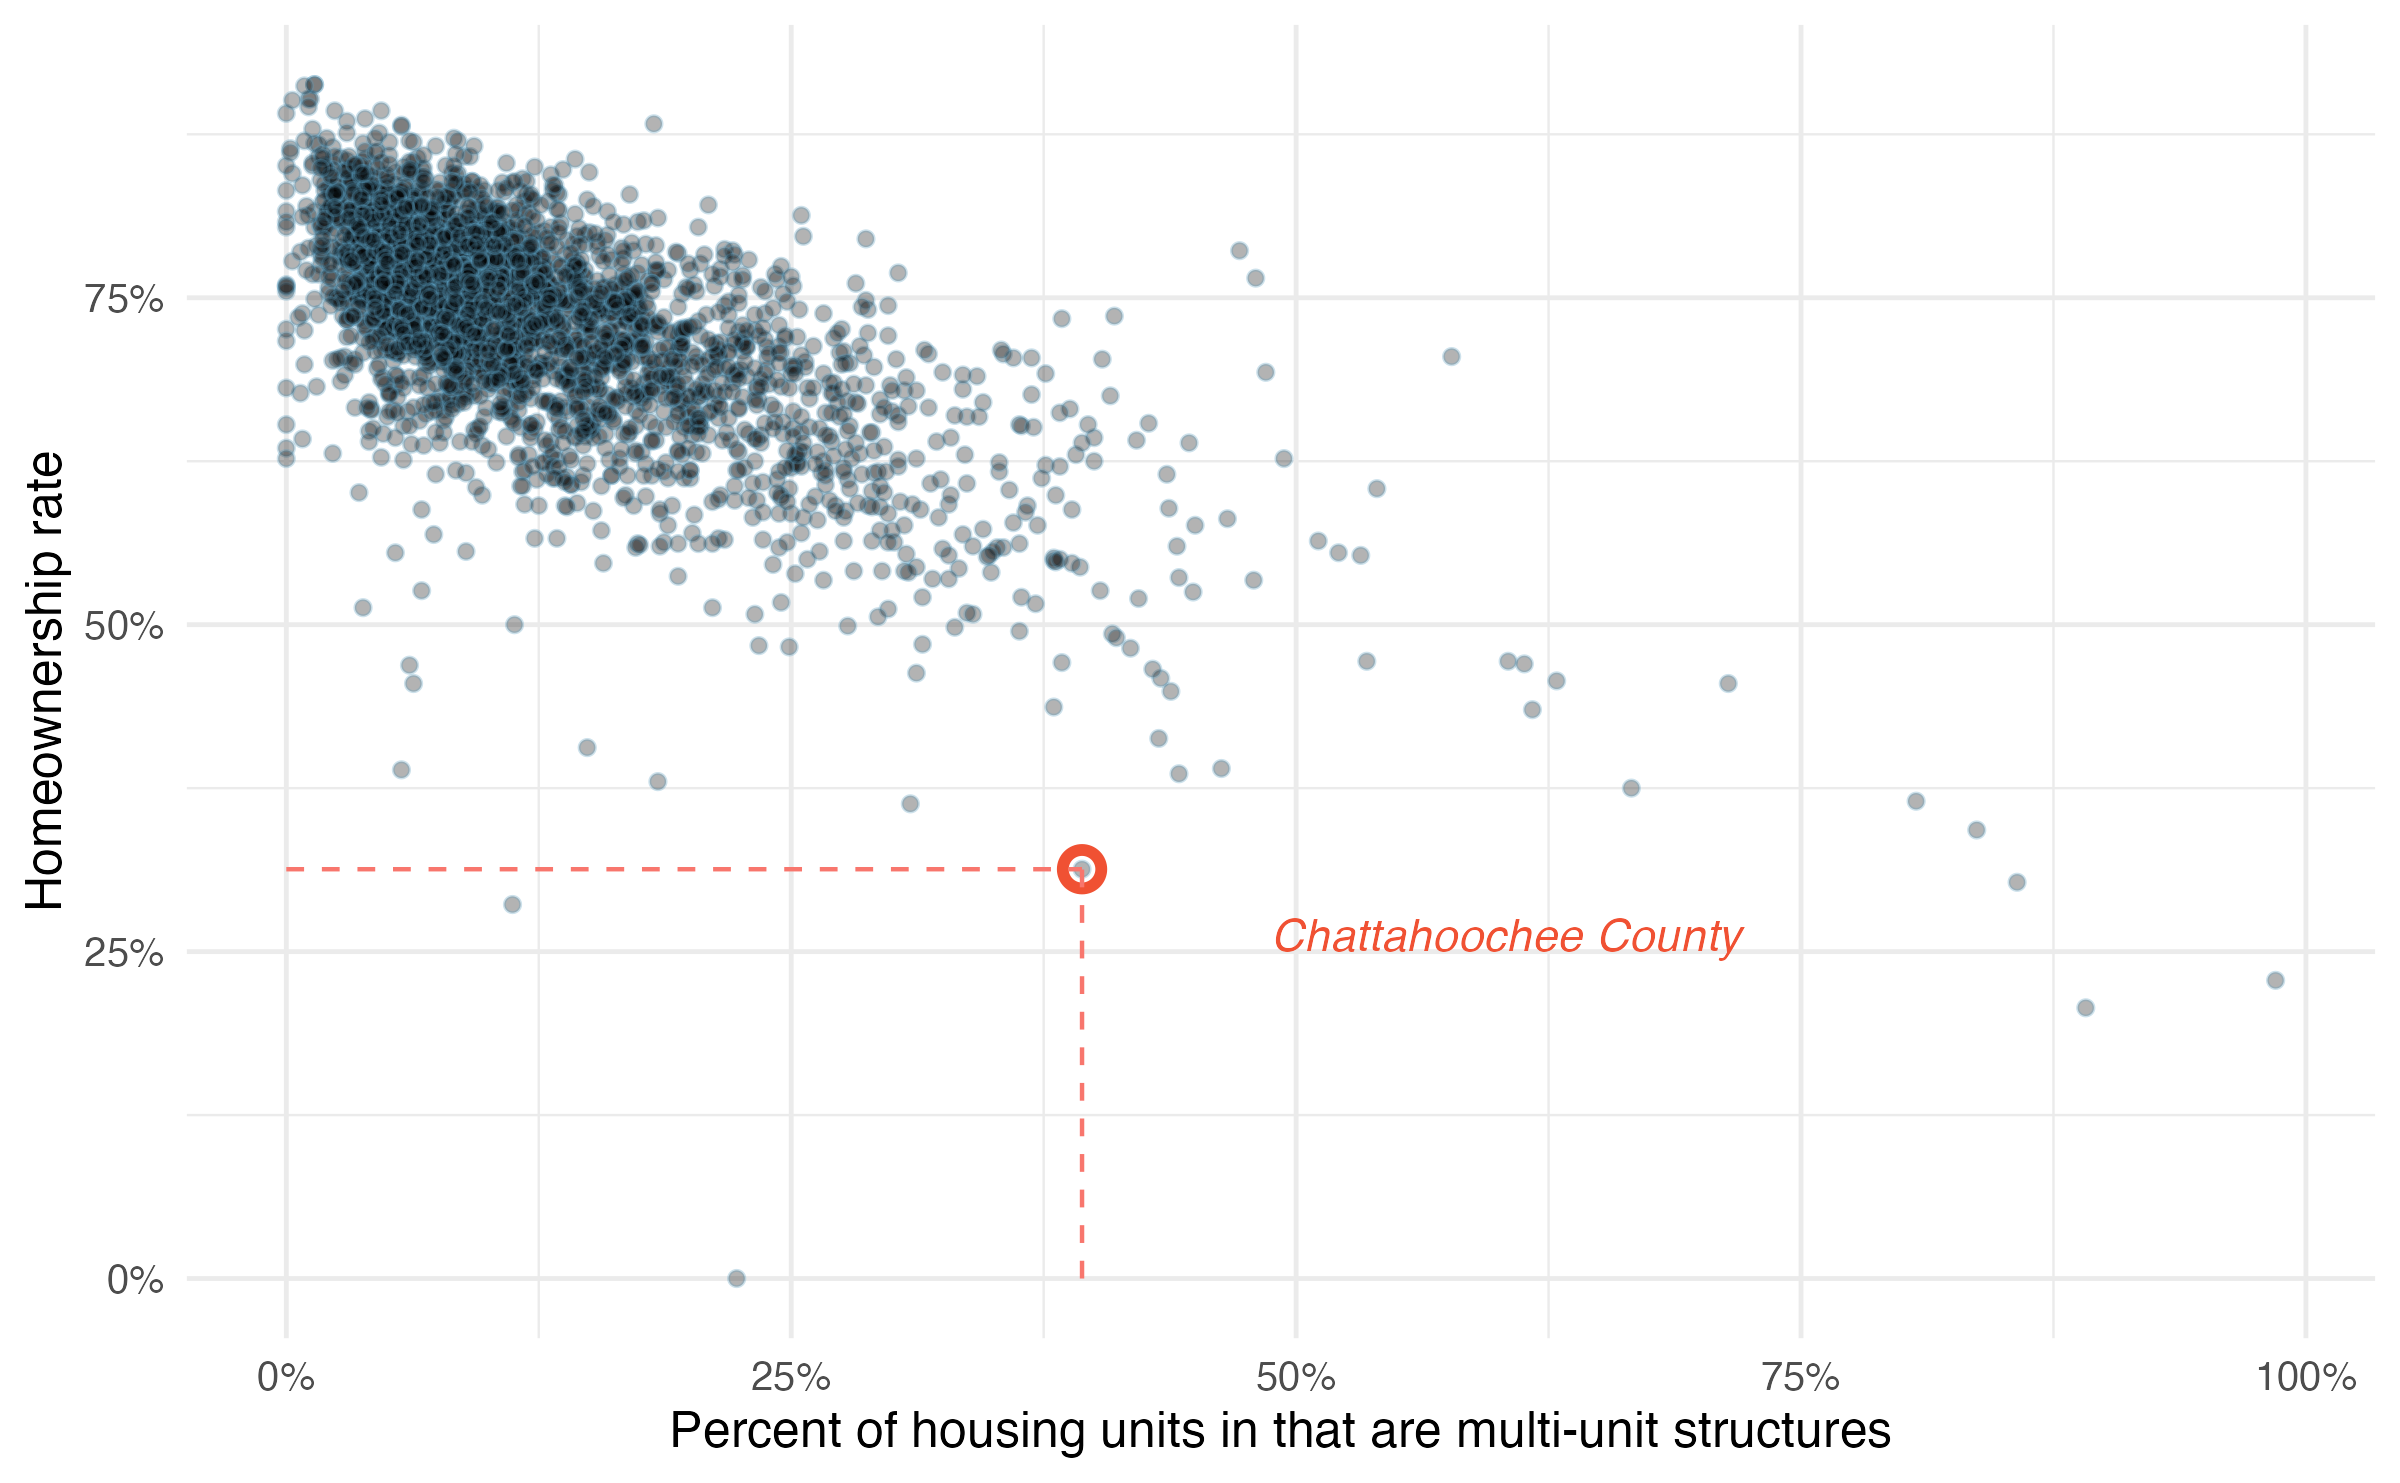
\includegraphics[width=0.8\textwidth,height=\textheight]{01-data-hello_files/figure-pdf/fig-county-multi-unit-homeownership-1.png}

}

\caption{\label{fig-county-multi-unit-homeownership}A scatterplot of
homeownership versus the percent of housing units that are in multi-unit
structures for US counties. The highlighted dot represents Chattahoochee
County, Georgia, which has a multi-unit rate of 39.4\% and a
homeownership rate of 31.3\%.}

\end{figure}%

The multi-unit and homeownership rates are said to be associated because
the plot shows a discernible pattern. When two variables show some
connection with one another, they are called
\textbf{associated}\index{association} variables.

\begin{guidedpractice}
Examine the variables in the \texttt{loan50} dataset, which are
described in Table~\ref{tbl-loan-50-variables}. Create two questions
about possible relationships between variables in \texttt{loan50} that
are of interest to you.\footnote{Two example questions: (1) What is the
  relationship between loan amount and total income? (2) If someone's
  income is above the average, will their interest rate tend to be above
  or below the average?}

\end{guidedpractice}

\begin{workedexample}
This example examines the relationship between the percent change in
population from 2010 to 2017 and median household income for counties,
which is visualized as a scatterplot in
Figure~\ref{fig-county-pop-change-med-hh-income}. Are these variables
associated?

\begin{center}\rule{0.5\linewidth}{0.5pt}\end{center}

The larger the median household income for a county, the higher the
population growth observed for the county. While it isn't true that
every county with a higher median household income has a higher
population growth, the trend in the plot is evident. Since there is some
relationship between the variables, they are associated.

\end{workedexample}

\begin{figure}[H]

\centering{

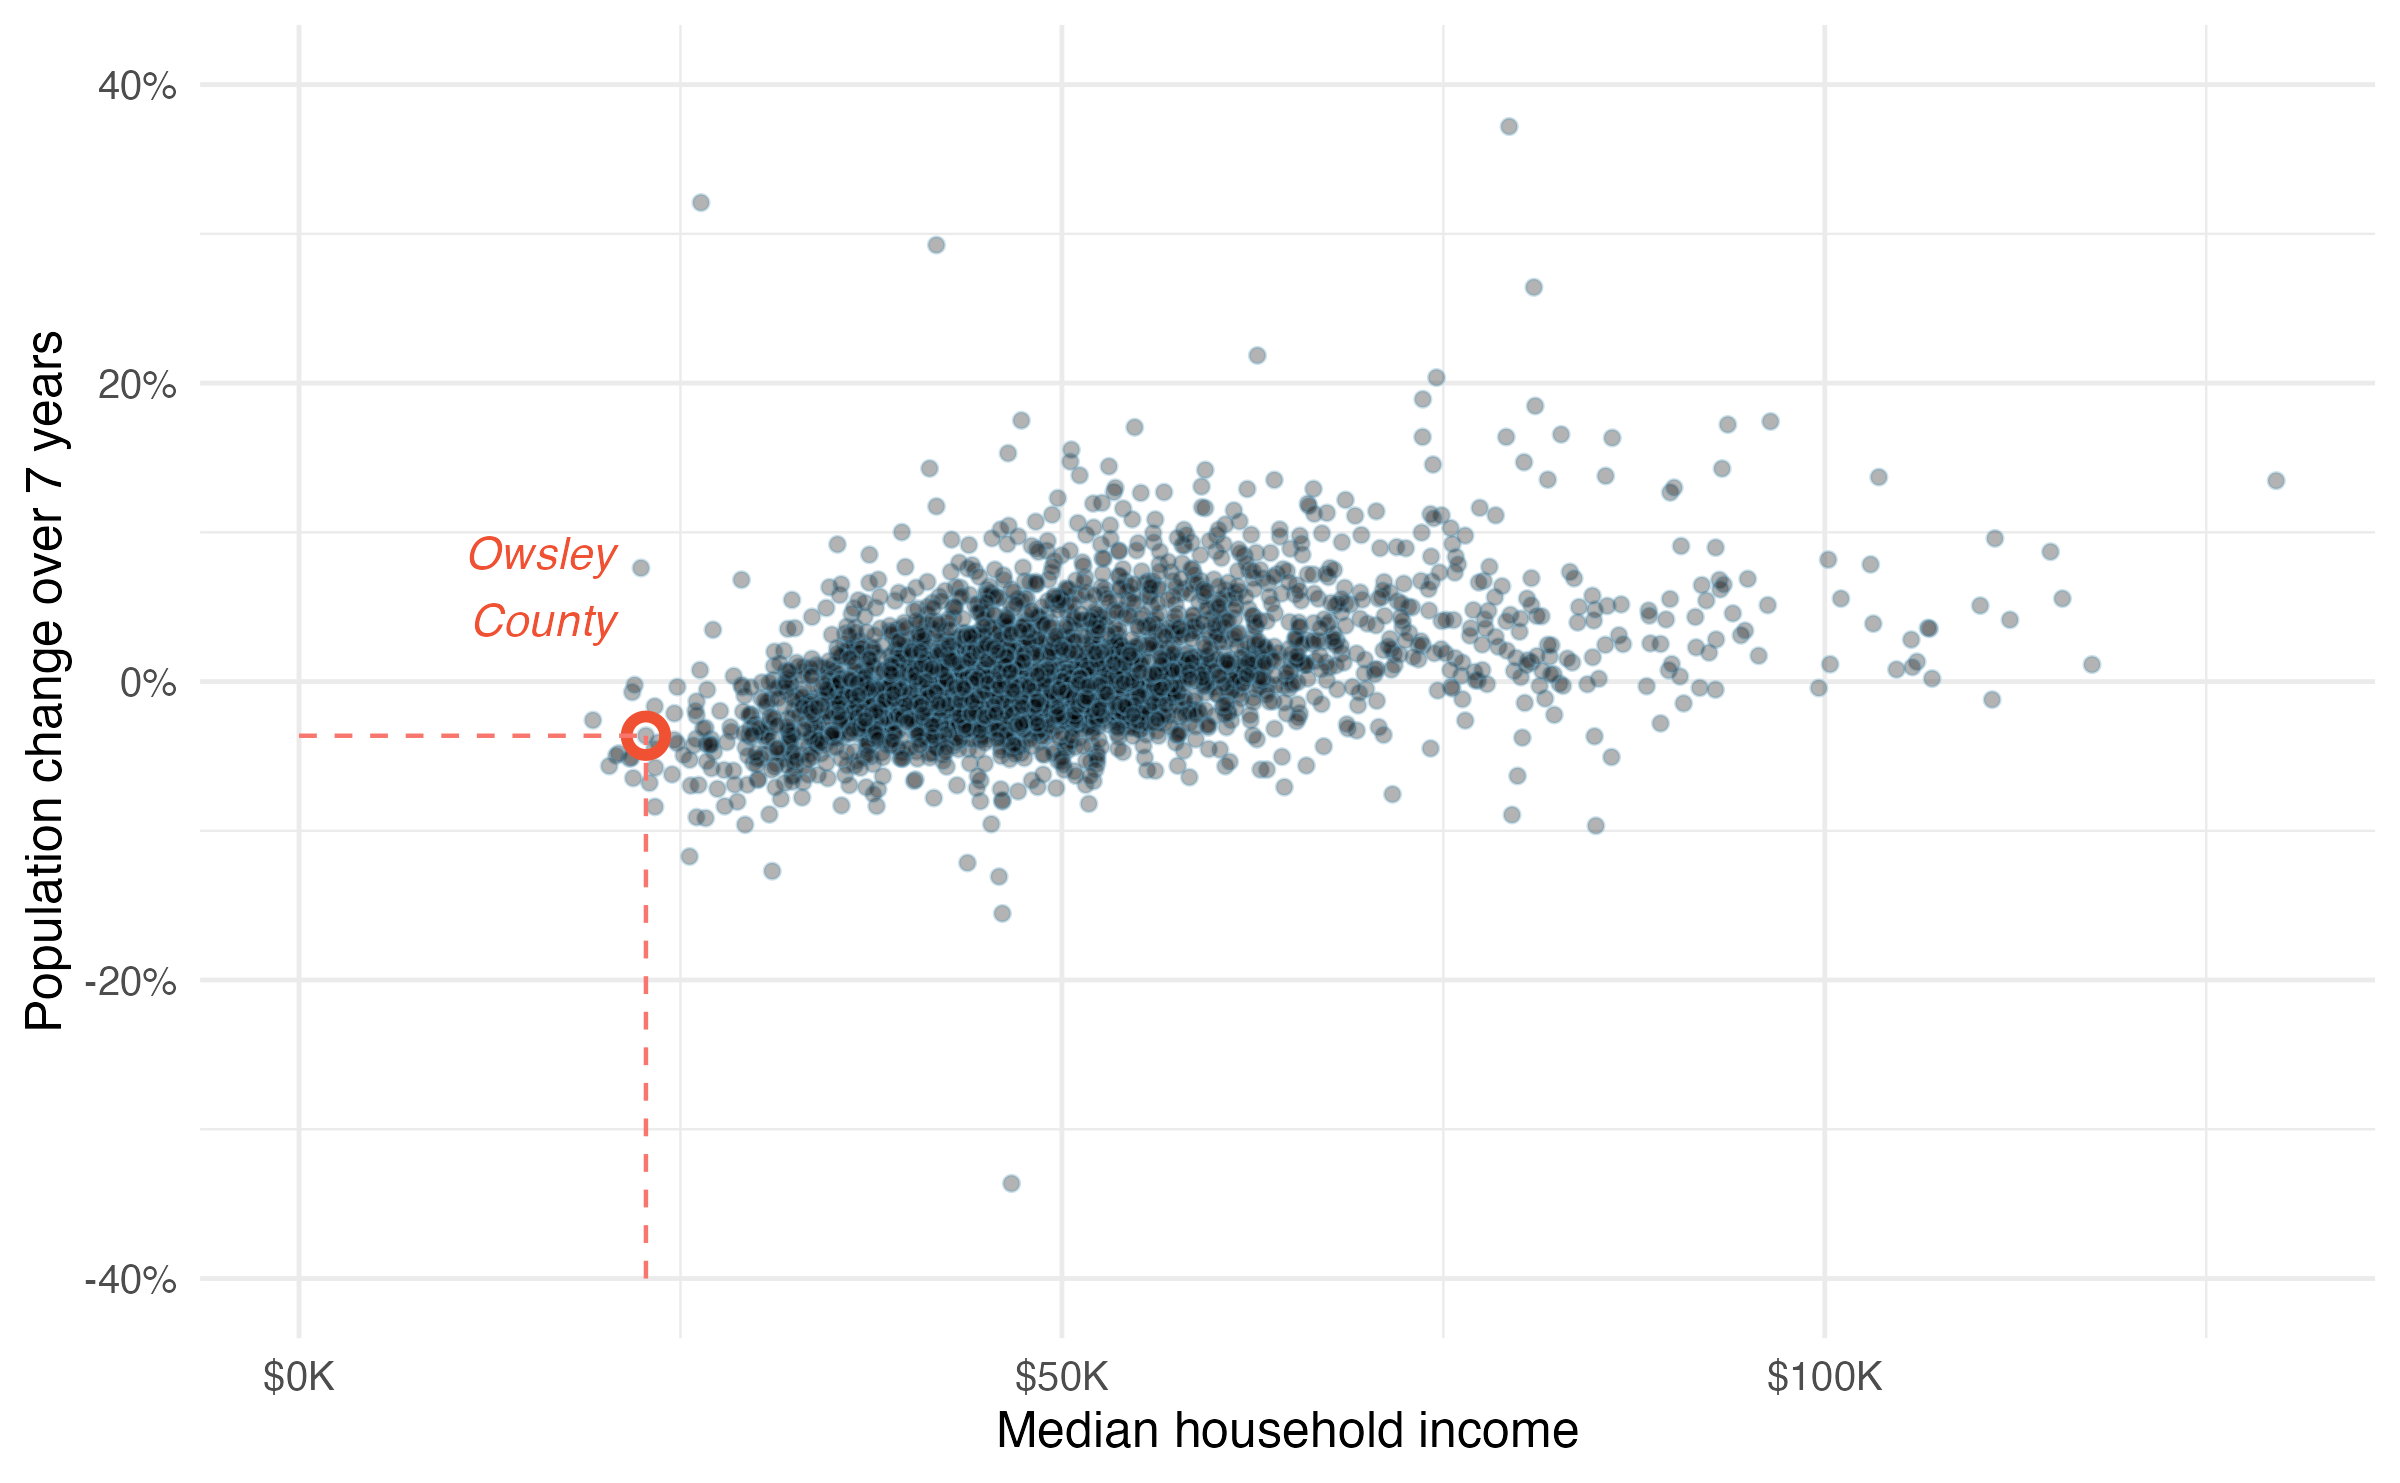
\includegraphics[width=0.8\textwidth,height=\textheight]{01-data-hello_files/figure-pdf/fig-county-pop-change-med-hh-income-1.png}

}

\caption{\label{fig-county-pop-change-med-hh-income}A scatterplot
showing population change against median household income. Owsley County
of Kentucky is highlighted, which lost 3.63\% of its population from
2010 to 2017 and had median household income of \$22,736.}

\end{figure}%

Because there is a downward trend in
Figure~\ref{fig-county-multi-unit-homeownership} -- counties with more
housing units that are in multi-unit structures are associated with
lower homeownership -- these variables are said to be \textbf{negatively
associated}\index{association}. A \textbf{positive
association}\index{association} is shown in the relationship between the
\texttt{median\_hh\_income} and \texttt{pop\_change} variables in
Figure~\ref{fig-county-pop-change-med-hh-income}, where counties with
higher median household income tend to have higher rates of population
growth.

If two variables are not associated, then they are said to be
\textbf{independent}\index{independence}. That is, two variables are
independent if there is no evident relationship between the two.

\begin{important}
\textbf{Associated or independent, not both.}

A pair of variables are either related in some way (associated) or not
(independent). No pair of variables is both associated and independent.

\end{important}

\subsection{Explanatory and response
variables}\label{explanatory-and-response-variables}

When we ask questions about the relationship between two variables, we
sometimes also want to determine if the change in one variable causes a
change in the other. Consider the following rephrasing of an earlier
question about the \texttt{county} dataset:

\begin{quote}
If there is an increase in the median household income in a county, does
this drive an increase in its population?
\end{quote}

In this question, we are asking whether one variable affects another. If
this is our underlying belief, then \emph{median household income} is
the \textbf{explanatory variable}\index{explanatory variable}, and the
\emph{population change} is the \textbf{response
variable}\index{response variable} in the hypothesized
relationship.\footnote{In some disciplines, it's customary to refer to
  the explanatory variable as the \textbf{independent variable} and the
  response variable as the \textbf{dependent variable}. However, this
  becomes confusing since a \emph{pair} of variables might be
  independent or dependent, so we avoid this language.}

\begin{important}
\textbf{Explanatory and response variables.}

When we suspect one variable might causally affect another, we label the
first variable the explanatory variable and the second the response
variable. We also use the terms \textbf{explanatory} and
\textbf{response} to describe variables where the \textbf{response}
might be predicted using the \textbf{explanatory} even if there is no
causal relationship.

explanatory variable \(\rightarrow\) \emph{might affect} \(\rightarrow\)
response variable

For many pairs of variables, there is no hypothesized relationship, and
these labels would not be applied to either variable in such cases.

\end{important}

Bear in mind that the act of labeling the variables in this way does
nothing to guarantee that a causal relationship exists. A formal
evaluation to check whether one variable causes a change in another
requires an experiment.

\subsection{Observational studies and
experiments}\label{observational-studies-and-experiments}

There are two primary types of data collection: experiments and
observational studies.

When researchers want to evaluate the effect of particular traits,
treatments, or conditions, they conduct an
\textbf{experiment}\index{study!experiment}. For instance, we may
suspect drinking a high-calorie energy drink will improve performance in
a race. To check if there really is a causal relationship between the
explanatory variable (whether the runner drank an energy drink or not)
and the response variable (the race time), researchers identify a sample
of individuals and split them into groups. The individuals in each group
are \emph{assigned} a treatment. When individuals are randomly assigned
to a group, the experiment is called a \textbf{randomized
experiment}\index{study!randomized experiment}. Random assignment
organizes the participants in a study into groups that are roughly equal
on all aspects, thus allowing us to control for any confounding
variables that might affect the outcome (e.g., fitness level, racing
experience, etc.). (See Section~\ref{sec-principles-experimental-design}
for more information on confounding variables.) For example, each runner
in the experiment could be randomly assigned, perhaps by flipping a
coin, into one of two groups: the first group receives a
\textbf{placebo}\index{placebo} (fake treatment, in this case a
no-calorie drink) and the second group receives the high-calorie energy
drink. See the case study in Section~\ref{sec-case-study-stents-strokes}
for another example of an experiment, though that study did not employ a
placebo.

Researchers perform an \textbf{observational
study}\index{study!observational} when they collect data in a way that
does not directly interfere with how the data arise. For instance,
researchers may collect information via surveys, review medical or
company records, or follow a \textbf{cohort}\index{cohort} of many
similar individuals to form hypotheses about why certain diseases might
develop. In each of these situations, researchers merely observe the
data that arise. In general, observational studies can provide evidence
of a naturally occurring association between variables, but they cannot
by themselves show a causal connection as they do not offer a mechanism
for controlling for confounding variables. (See
Section~\ref{sec-principles-experimental-design} for more information on
confounding variables.)

\begin{important}
\textbf{Association} \(\neq\) \textbf{Causation.}

In general, association does not imply causation. An advantage of a
randomized experiment is that it is easier to establish causal
relationships with such a study. The main reason for this is that
observational studies do not control for confounding variables, and
hence establishing causal relationships with observational studies
requires advanced statistical methods (that are beyond the scope of this
book). We revisit ideas of confounding when we discuss experiments in
Section~\ref{sec-principles-experimental-design}.

\end{important}

\vspace{10mm}

\section{Chapter review}\label{sec-chp1-review}

\subsection{Summary}\label{summary}

This chapter introduced you to the world of data. Data can be organized
in many ways but tidy data, where each row represents an observation and
each column represents a variable, lends itself most easily to
statistical analysis. Many of the ideas from this chapter will be
revisited as we move on to doing end-to-end data analyses. In the next
chapter you're going to learn about how we can design studies to collect
the data we need to make conclusions with the desired scope of
inference.

\subsection{Terms}\label{terms}

The terms introduced in this chapter are presented in
Table~\ref{tbl-terms-chp-1}. If you're not sure what some of these terms
mean, we recommend you go back in the text and review their definitions.
You should be able to easily spot them as \textbf{bolded text}.

\begin{table}[H]

\caption{\label{tbl-terms-chp-1}Terms introduced in this chapter.}

\centering{

\centering
\begin{tabular}[t]{>{\raggedright\arraybackslash}p{12em}>{\raggedright\arraybackslash}p{12em}>{\raggedright\arraybackslash}p{12em}}
\toprule
\cellcolor{gray!10}{associated} & \cellcolor{gray!10}{experiment} & \cellcolor{gray!10}{ordinal}\\
case & explanatory variable & placebo\\
\cellcolor{gray!10}{categorical} & \cellcolor{gray!10}{independent} & \cellcolor{gray!10}{positive association}\\
cohort & level & randomized experiment\\
\cellcolor{gray!10}{continuous} & \cellcolor{gray!10}{negative association} & \cellcolor{gray!10}{response variable}\\
data & nominal & summary statistic\\
\cellcolor{gray!10}{data frame} & \cellcolor{gray!10}{numerical} & \cellcolor{gray!10}{tidy data}\\
dependent & observation & unit of observation\\
\cellcolor{gray!10}{discrete} & \cellcolor{gray!10}{observational study} & \cellcolor{gray!10}{variable}\\
\bottomrule
\end{tabular}

}

\end{table}%

\clearpage

\section{Exercises}\label{sec-chp1-exercises}

Answers to odd-numbered exercises can be found in
Appendix~\ref{sec-exercise-solutions-01}.

\begin{exercises}

\begin{enumerate}
\def\labelenumi{\arabic{enumi}.}
\item
  \textbf{Marvel Cinematic Universe films.} The data frame below
  contains information on Marvel Cinematic Universe films through the
  Infinity saga (a movie storyline spanning from Ironman in 2008 to
  Endgame in 2019). Box office totals are given in millions of US
  Dollars. How many observations and how many variables does this data
  frame have?\footnote{The
    \href{http://openintrostat.github.io/openintro/reference/mcu_films.html}{\texttt{mcu\_films}}
    data used in this exercise can be found in the
    \href{http://openintrostat.github.io/openintro}{\textbf{openintro}}
    R package.}

  \begin{table}[H]
  \centering
  \begin{tabular}[t]{c>{\raggedright\arraybackslash}p{10em}cccccc}
  \toprule
  \multicolumn{2}{c}{ } & \multicolumn{2}{c}{Length} & \multicolumn{2}{c}{ } & \multicolumn{2}{c}{Gross} \\
  \cmidrule(l{3pt}r{3pt}){3-4} \cmidrule(l{3pt}r{3pt}){7-8}
    & Title & Hrs & Mins & Release Date & Opening Wknd US & US & World\\
  \midrule
  1 & Iron Man & 2 & 6 & 5/2/2008 & 98.62 & 319.03 & 585.8\\
  2 & The Incredible Hulk & 1 & 52 & 6/12/2008 & 55.41 & 134.81 & 264.77\\
  3 & Iron Man 2 & 2 & 4 & 5/7/2010 & 128.12 & 312.43 & 623.93\\
  4 & Thor & 1 & 55 & 5/6/2011 & 65.72 & 181.03 & 449.33\\
  5 & Captain America: The First Avenger & 2 & 4 & 7/22/2011 & 65.06 & 176.65 & 370.57\\
  ... & ... & ... & ... & ... & ... & ... & ...\\
  23 & Spiderman: Far from Home & 2 & 9 & 7/2/2019 & 92.58 & 390.53 & 1131.93\\
  \bottomrule
  \end{tabular}
  \end{table}
\end{enumerate}

\vspace{10mm}

\begin{enumerate}
\def\labelenumi{\arabic{enumi}.}
\setcounter{enumi}{1}
\item
  \textbf{Cherry Blossom Run.} The data frame below contains information
  on runners in the 2017 Cherry Blossom Run, which is an annual road
  race that takes place in Washington, DC. Most runners participate in a
  10-mile run while a smaller fraction take part in a 5k run or walk.
  How many observations and how many variables does this data frame
  have?\footnote{The
    \href{http://openintrostat.github.io/openintro/reference/run17.html}{\texttt{run17}}
    data used in this exercise can be found in the
    \href{http://openintrostat.github.io/cherryblossom}{\textbf{cherryblossom}}
    R package.}

  \begin{table}[H]
  \centering
  \begin{tabular}[t]{llllclcccl}
  \toprule
  \multicolumn{6}{c}{ } & \multicolumn{2}{c}{Time} & \multicolumn{2}{c}{ } \\
  \cmidrule(l{3pt}r{3pt}){7-8}
    & Bib & Name & Sex & Age & City / Country & Net & Clock & Pace & Event\\
  \midrule
  1 & 6 & Hiwot G. & F & 21 & Ethiopia & 3217 & 3217 & 321 & 10 Mile\\
  2 & 22 & Buze D. & F & 22 & Ethiopia & 3232 & 3232 & 323 & 10 Mile\\
  3 & 16 & Gladys K. & F & 31 & Kenya & 3276 & 3276 & 327 & 10 Mile\\
  4 & 4 & Mamitu D. & F & 33 & Ethiopia & 3285 & 3285 & 328 & 10 Mile\\
  5 & 20 & Karolina N. & F & 35 & Poland & 3288 & 3288 & 328 & 10 Mile\\
  ... & ... & ... & ... & ... & ... & ... & ... & ... & ...\\
  19961 & 25153 & Andres E. & M & 33 & Woodbridge, VA & 5287 & 5334 & 1700 & 5K\\
  \bottomrule
  \end{tabular}
  \end{table}
\end{enumerate}

\clearpage

\begin{enumerate}
\def\labelenumi{\arabic{enumi}.}
\setcounter{enumi}{2}
\item
  \textbf{Air pollution and birth outcomes, study components.}
  Researchers collected data to examine the relationship between air
  pollutants and preterm births in Southern California. During the study
  air pollution levels were measured by air quality monitoring stations.
  Specifically, levels of carbon monoxide were recorded in parts per
  million, nitrogen dioxide and ozone in parts per hundred million, and
  coarse particulate matter (PM\(_{10}\)) in \(\mu g/m^3\). Length of
  gestation data were collected on 143,196 births between the years 1989
  and 1993, and air pollution exposure during gestation was calculated
  for each birth. The analysis suggested that increased ambient
  PM\(_{10}\) and, to a lesser degree, CO concentrations may be
  associated with the occurrence of preterm births. (Ritz et al. 2000)

  \begin{enumerate}
  \def\labelenumii{\alph{enumii}.}
  \item
    Identify the main research question of the study.
  \item
    Who are the subjects in this study, and how many are included?
  \item
    What are the variables in the study? Identify each variable as
    numerical or categorical. If numerical, state whether the variable
    is discrete or continuous. If categorical, state whether the
    variable is ordinal.
  \end{enumerate}
\end{enumerate}

\vspace{10mm}

\begin{enumerate}
\def\labelenumi{\arabic{enumi}.}
\setcounter{enumi}{3}
\item
  \textbf{Cheaters, study components.} Researchers studying the
  relationship between honesty, age and self-control conducted an
  experiment on 160 children between the ages of 5 and 15. Participants
  reported their age, sex, and whether they were an only child or not.
  The researchers asked each child to toss a fair coin in private and to
  record the outcome (white or black) on a paper sheet, and said they
  would only reward children who report white. (Bucciol and Piovesan
  2011)

  \begin{enumerate}
  \def\labelenumii{\alph{enumii}.}
  \item
    Identify the main research question of the study.
  \item
    Who are the subjects in this study, and how many are included?
  \item
    The study's findings can be summarized as follows: \emph{``Half the
    students were explicitly told not to cheat and the others were not
    given any explicit instructions. In the no instruction group
    probability of cheating was found to be uniform across groups based
    on child's characteristics. In the group that was explicitly told to
    not cheat, girls were less likely to cheat, and while rate of
    cheating didn't vary by age for boys, it decreased with age for
    girls.''} How many variables were recorded for each subject in the
    study in order to conclude these findings? State the variables and
    their types.
  \end{enumerate}
\end{enumerate}

\clearpage

\begin{enumerate}
\def\labelenumi{\arabic{enumi}.}
\setcounter{enumi}{4}
\item
  \textbf{Gamification and statistics, study components.} Gamification
  is the application of game-design elements and game principles in
  non-game contexts. In educational settings, gamification is often
  implemented as educational activities to solve problems by using
  characteristics of game elements. Researchers investigating the
  effects of gamification on learning statistics conducted a study where
  they split college students in a statistics class into four groups:
  (1) no reading exercises and no gamification, (2) reading exercises
  but no gamification, (3) gamification but no reading exercises, and
  (4) gamification and reading exercises. Students in all groups also
  attended lectures. Students in the class were from two majors:
  Electrical and Computer Engineering (n = 279) and Business
  Administration (n = 86). After their assigned learning experience,
  each student took a final evaluation comprised of 30 multiple choice
  question and their score was measured as the number of questions they
  answered correctly. The researchers considered students' gender, level
  of studies (first through fourth year) and academic major. Other
  variables considered were expertise in the English language and use of
  personal computers and games, both of which were measured on a scale
  of 1 (beginner) to 5 (proficient). The study found that gamification
  had a positive effect on student learning compared to traditional
  teaching methods involving lectures and reading exercises. They also
  found that the effect was larger for females and Engineering students.
  (Legaki et al. 2020)

  \begin{enumerate}
  \def\labelenumii{\alph{enumii}.}
  \item
    Identify the main research question of the study.
  \item
    Who were the subjects in this study, and how many were included?
  \item
    What are the variables in the study? Identify each variable as
    numerical or categorical. If numerical, state whether the variable
    is discrete or continuous. If categorical, state whether the
    variable is ordinal.
  \end{enumerate}
\end{enumerate}

\vspace{10mm}

\begin{enumerate}
\def\labelenumi{\arabic{enumi}.}
\setcounter{enumi}{5}
\item
  \textbf{Stealers, study components.} In a study of the relationship
  between socio-economic class and unethical behavior, 129 University of
  California undergraduates at Berkeley were asked to identify
  themselves as having low or high social-class by comparing themselves
  to others with the most (least) money, most (least) education, and
  most (least) respected jobs. They were also presented with a jar of
  individually wrapped candies and informed that the candies were for
  children in a nearby laboratory, but that they could take some if they
  wanted. After completing some unrelated tasks, participants reported
  the number of candies they had taken. (Piff et al. 2012)

  \begin{enumerate}
  \def\labelenumii{\alph{enumii}.}
  \item
    Identify the main research question of the study.
  \item
    Who were the subjects in this study, and how many were included?
  \item
    The study found that students who were identified as upper-class
    took more candy than others. How many variables were recorded for
    each subject in the study in order to conclude these findings? State
    the variables and their types.
  \end{enumerate}
\end{enumerate}

\clearpage

\begin{enumerate}
\def\labelenumi{\arabic{enumi}.}
\setcounter{enumi}{6}
\item
  \textbf{Migraine and acupuncture.} A migraine is a particularly
  painful type of headache, which patients sometimes wish to treat with
  acupuncture. To determine whether acupuncture relieves migraine pain,
  researchers conducted a randomized controlled study where 89
  individuals who identified as female diagnosed with migraine headaches
  were randomly assigned to one of two groups: treatment or control.
  Forty-three (43) patients in the treatment group received acupuncture
  that is specifically designed to treat migraines. Forty-six (46)
  patients in the control group received placebo acupuncture (needle
  insertion at non-acupoint locations). Twenty-four (24) hours after
  patients received acupuncture, they were asked if they were pain free.
  Results are summarized in the contingency table below. Also provided
  is a figure from the original paper displaying the appropriate area
  (M) versus the inappropriate area (S) used in the treatment of
  migraine attacks. \footnote{The
    \href{http://openintrostat.github.io/openintro/reference/migraine.html}{\texttt{migraine}}
    data used in this exercise can be found in the
    \href{http://openintrostat.github.io/openintro}{\textbf{openintro}}
    R package.} (Allais et al. 2011)

  \begin{table}[H]
  \centering
  \begin{tabular}[t]{>{\raggedright\arraybackslash}p{5em}>{\raggedleft\arraybackslash}p{5em}>{\raggedleft\arraybackslash}p{5em}}
  \toprule
  \multicolumn{1}{c}{} & \multicolumn{2}{c}{Pain free?} \\
  \cmidrule(l{3pt}r{3pt}){2-3}
  Group & No & Yes\\
  \midrule
  Control & 44 & 2\\
  Treatment & 33 & 10\\
  \bottomrule
  \end{tabular}
  \end{table}

  \begin{enumerate}
  \def\labelenumii{\alph{enumii}.}
  \item
    What percent of patients in the treatment group were pain free 24
    hours after receiving acupuncture?
  \item
    What percent were pain free in the control group?
  \item
    In which group did a higher percent of patients become pain free 24
    hours after receiving acupuncture?
  \item
    Your findings so far might suggest that acupuncture is an effective
    treatment for migraines for all people who suffer from migraines.
    However this is not the only possible conclusion. What is one other
    possible explanation for the observed difference between the
    percentages of patients that are pain free 24 hours after receiving
    acupuncture in the two groups?
  \item
    What are the explanatory and response variables in this study?
  \end{enumerate}
\item
  \textbf{Sinusitis and antibiotics.} Researchers studying the effect of
  antibiotic treatment for acute sinusitis compared to symptomatic
  treatments randomly assigned 166 adults diagnosed with acute sinusitis
  to one of two groups: treatment or control. Study participants
  received either a 10-day course of amoxicillin (an antibiotic) or a
  placebo similar in appearance and taste. The placebo consisted of
  symptomatic treatments such as acetaminophen, nasal decongestants,
  etc. At the end of the 10-day period, patients were asked if they
  experienced improvement in symptoms. The distribution of responses is
  summarized below.\footnote{The
    \href{http://openintrostat.github.io/openintro/reference/sinusitis.html}{\texttt{sinusitis}}
    data used in this exercise can be found in the
    \href{http://openintrostat.github.io/openintro}{\textbf{openintro}}
    R package.} (Garbutt et al. 2012)

  \begin{table}[H]
  \centering
  \begin{tabular}[t]{>{\raggedright\arraybackslash}p{5em}>{\raggedleft\arraybackslash}p{5em}>{\raggedleft\arraybackslash}p{5em}}
  \toprule
  \multicolumn{1}{c}{} & \multicolumn{2}{c}{Improvement} \\
  \cmidrule(l{3pt}r{3pt}){2-3}
  Group & No & Yes\\
  \midrule
  Control & 16 & 65\\
  Treatment & 19 & 66\\
  \bottomrule
  \end{tabular}
  \end{table}

  \begin{enumerate}
  \def\labelenumii{\alph{enumii}.}
  \item
    What percent of patients in the treatment group experienced
    improvement in symptoms?
  \item
    What percent experienced improvement in symptoms in the control
    group?
  \item
    In which group did a higher percentage of patients experience
    improvement in symptoms?
  \item
    Your findings so far might suggest a real difference in the
    effectiveness of antibiotic and placebo treatments for improving
    symptoms of sinusitis. However this is not the only possible
    conclusion. What is one other possible explanation for the observed
    difference between the percentages patients who experienced
    improvement in symptoms?
  \item
    What are the explanatory and response variables in this study?
  \end{enumerate}
\end{enumerate}

\vspace{10mm}

\begin{enumerate}
\def\labelenumi{\arabic{enumi}.}
\setcounter{enumi}{8}
\item
  \textbf{Daycare fines, study components.} Researchers tested the
  deterrence hypothesis which predicts that the introduction of a
  penalty will reduce the occurrence of the behavior subject to the
  fine, with the condition that the fine leaves everything else
  unchanged, by instituting a fine for late pickup at daycare centers.
  For this study, they worked with 10 volunteer daycare centers that did
  not originally impose a fine to parents for picking up their kids
  late. They randomly selected 6 of these daycare centers and instituted
  a monetary fine (of a considerable amount) for picking up children
  late and then removed it. In the remaining 4 daycare centers no fine
  was introduced. The study period was divided into four: before the
  fine (weeks 1--4), the first 4 weeks with the fine (weeks 5-8), the
  last 8 weeks with fine (weeks 9--16), and the after fine period (weeks
  17-20). Throughout the study, the number of kids who were picked up
  late was recorded each week for each daycare. The study found that the
  number of late-coming parents increased discernibly when the fine was
  introduced, and no reduction occurred after the fine was
  removed.\footnote{The
    \href{http://openintrostat.github.io/openintro/reference/daycare_fines.html}{\texttt{daycare\_fines}}
    data used in this exercise can be found in the
    \href{http://openintrostat.github.io/openintro}{\textbf{openintro}}
    R package.} (Gneezy and Rustichini 2000)

  \begin{table}[H]
  \centering
  \begin{tabular}[t]{cclcl}
  \toprule
  center & week & group & late\_pickups & study\_period\\
  \midrule
  1 & 1 & test & 8 & before fine\\
  1 & 2 & test & 8 & before fine\\
  1 & 3 & test & 7 & before fine\\
  1 & 4 & test & 6 & before fine\\
  1 & 5 & test & 8 & first 4 weeks with fine\\
  ... & ... & ... & ... & ...\\
  10 & 20 & control & 13 & after fine\\
  \bottomrule
  \end{tabular}
  \end{table}

  \begin{enumerate}
  \def\labelenumii{\alph{enumii}.}
  \item
    Is this an observational study or an experiment? Explain your
    reasoning.
  \item
    What are the cases in this study and how many are included?
  \item
    What is the response variable in the study and what type of variable
    is it?
  \item
    What are the explanatory variables in the study and what types of
    variables are they?
  \end{enumerate}
\end{enumerate}

\clearpage

\begin{enumerate}
\def\labelenumi{\arabic{enumi}.}
\setcounter{enumi}{9}
\item
  \textbf{Efficacy of COVID-19 vaccine on adolescents, study
  components.} Results of a Phase 3 trial announced in March 2021 show
  that the Pfizer-BioNTech COVID-19 vaccine demonstrated 100\% efficacy
  and robust antibody responses on 12 to 15 years old adolescents with
  or without prior evidence of SARS-CoV-2 infection. In this trial 2,260
  adolescents were randomly assigned to two groups: one group got the
  vaccine (n = 1,131) and the other got a placebo (n = 1,129). While 18
  cases of COVID-19 were observed in the placebo group, none were
  observed in the vaccine group.\footnote{The
    \href{http://openintrostat.github.io/openintro/reference/biontech_adolescents.html}{\texttt{biontech\_adolescents}}
    data used in this exercise can be found in the
    \href{http://openintrostat.github.io/openintro}{\textbf{openintro}}
    R package.} (Pfizer 2021)

  \begin{enumerate}
  \def\labelenumii{\alph{enumii}.}
  \item
    Is this an observational study or an experiment? Explain your
    reasoning.
  \item
    What are the cases in this study and how many are included?
  \item
    What is the response variable in the study and what type of variable
    is it?
  \item
    What are the explanatory variables in the study and what types of
    variables are they?
  \end{enumerate}
\item
  \textbf{Palmer penguins.} Data were collected on 344 penguins living
  on three islands (Torgersen, Biscoe, and Dream) in the Palmer
  Archipelago, Antarctica. In addition to which island each penguin
  lives on, the data contains information on the species of the penguin
  (\emph{Adelie}, \emph{Chinstrap}, or \emph{Gentoo}), its bill length,
  bill depth, and flipper length (measured in millimeters), its body
  mass (measured in grams), and the sex of the penguin (female or male).
  \footnote{Artwork by \href{https://twitter.com/allison_horst}{Allison
    Horst}.} (Gorman, Williams, and Fraser 2014)

  \begin{enumerate}
  \def\labelenumii{\alph{enumii}.}
  \tightlist
  \item
    How many cases were included in the data?
  \item
    How many numerical variables are included in the data? Indicate what
    they are, and if they are continuous or discrete.
  \item
    How many categorical variables are included in the data, and what
    are they? List the corresponding levels (categories) for each.
  \end{enumerate}
\item
  \textbf{Smoking habits of UK residents.} A survey was conducted to
  study the smoking habits of 1,691 UK residents. Below is a data frame
  displaying a portion of the data collected in this survey. A blank
  cell indicates that data for that variable was not available for a
  given respondent.\footnote{The
    \href{http://openintrostat.github.io/openintro/reference/smoking.html}{\texttt{smoking}}
    data used in this exercise can be found in the
    \href{http://openintrostat.github.io/openintro}{\textbf{openintro}}
    R package.}

  \begin{table}[H]
  \centering
  \begin{tabular}[t]{llllclcc}
  \toprule
  \multicolumn{6}{c}{ } & \multicolumn{2}{c}{amount} \\
  \cmidrule(l{3pt}r{3pt}){7-8}
    & sex & age & marital\_status & gross\_income & smoke & weekend & weekday\\
  \midrule
  1 & Female & 61 & Married & 2,600 to 5,200 & No &  & \\
  2 & Female & 61 & Divorced & 10,400 to 15,600 & Yes & 5 & 4\\
  3 & Female & 69 & Widowed & 5,200 to 10,400 & No &  & \\
  4 & Female & 50 & Married & 5,200 to 10,400 & No &  & \\
  5 & Male & 31 & Single & 10,400 to 15,600 & Yes & 10 & 20\\
  ... & ... & ... & ... & ... & ... &  & \\
  1691 & Male & 49 & Divorced & Above 36,400 & Yes & 15 & 10\\
  \bottomrule
  \end{tabular}
  \end{table}

  \begin{enumerate}
  \def\labelenumii{\alph{enumii}.}
  \item
    What does each row of the data frame represent?
  \item
    How many participants were included in the survey?
  \item
    Indicate whether each variable is numerical or categorical. If
    numerical, identify as continuous or discrete. If categorical,
    indicate if the variable is ordinal.
  \end{enumerate}
\end{enumerate}

\clearpage

\begin{enumerate}
\def\labelenumi{\arabic{enumi}.}
\setcounter{enumi}{12}
\item
  \textbf{US Airports.} The visualization below shows the geographical
  distribution of airports in the contiguous United States and
  Washington, DC. This visualization was constructed based on a dataset
  where each observation is an airport.\footnote{The
    \href{http://openintrostat.github.io/airports/reference/usairports.html}{\texttt{usairports}}
    data used in this exercise can be found in the
    \href{http://openintrostat.github.io/airports/}{\textbf{airports}} R
    package.}

  \vspace{-1mm}

  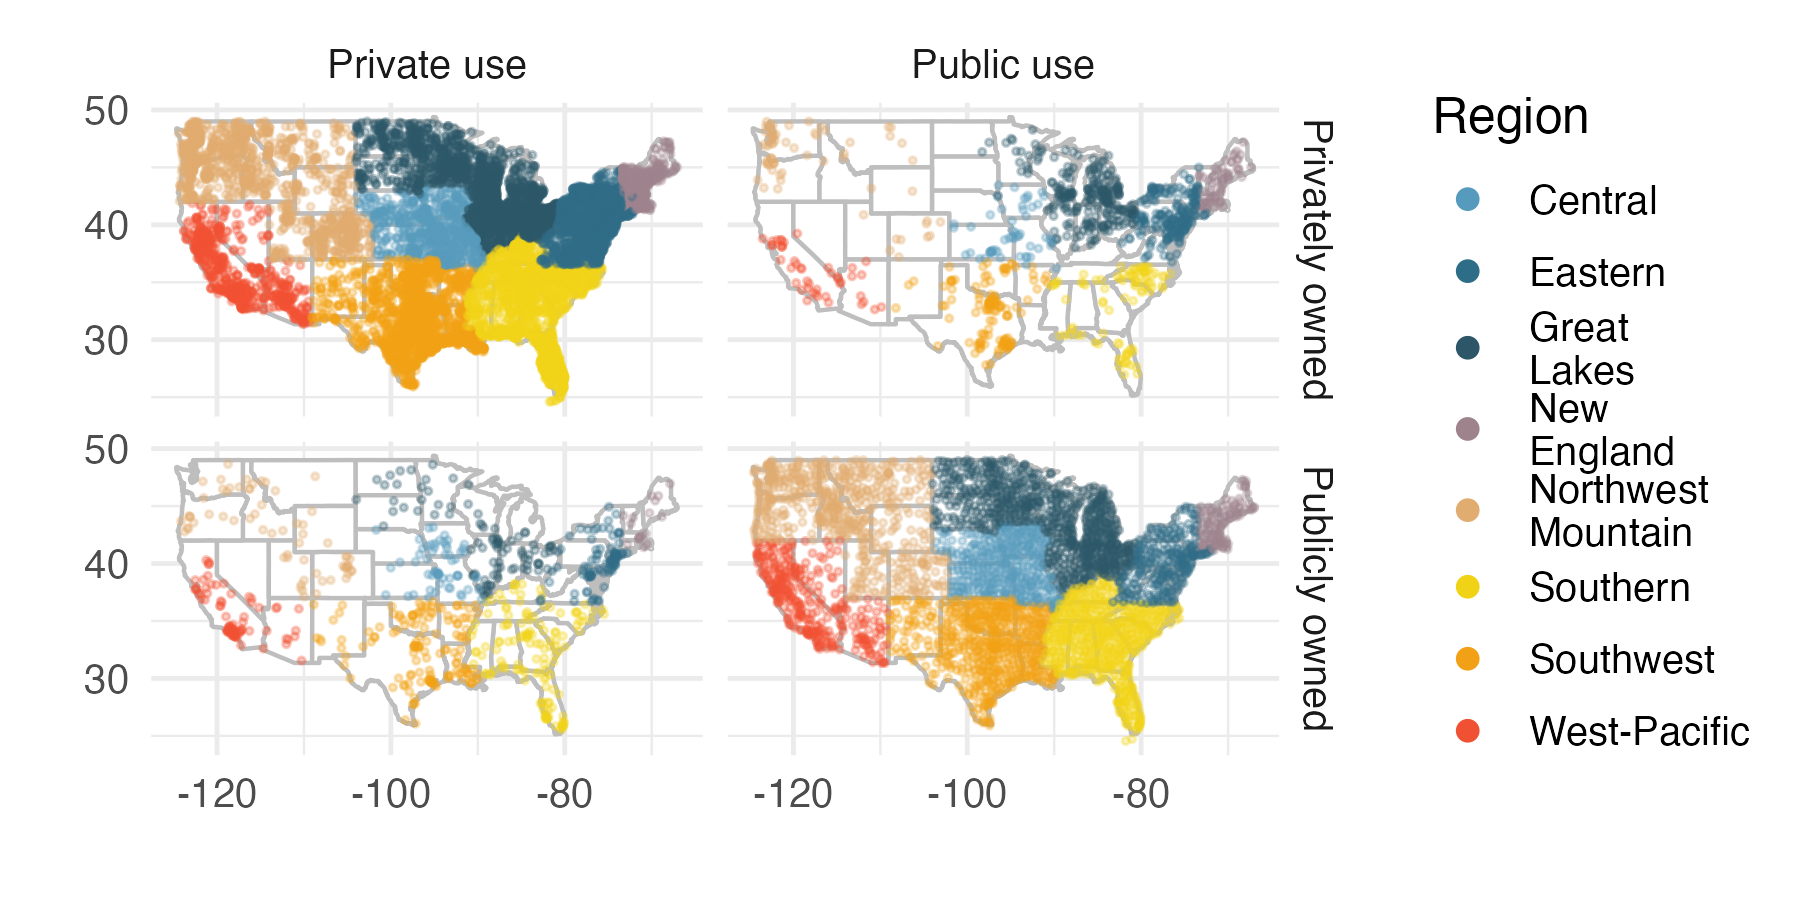
\includegraphics[width=1\textwidth,height=\textheight]{01-data-hello_files/figure-pdf/unnamed-chunk-32-1.png}

  \vspace{-5mm}

  \begin{enumerate}
  \def\labelenumii{\alph{enumii}.}
  \item
    List the variables you believe were necessary to create this
    visualization.
  \item
    Indicate whether each variable is numerical or categorical. If
    numerical, identify as continuous or discrete. If categorical,
    indicate if the variable is ordinal.
  \end{enumerate}
\item
  \textbf{UN Votes.} The visualization below shows voting patterns in
  the United States, Canada, and Mexico in the United Nations General
  Assembly on a variety of issues. Specifically, for a given year
  between 1946 and 2019, it displays the percentage of roll calls in
  which the country voted yes for each issue. This visualization was
  constructed based on a dataset where each observation is a
  country/year pair.\footnote{The data used in this exercise can be
    found in the
    \href{https://cran.r-project.org/web/packages/unvotes/index.html}{\textbf{unvotes}}
    R package.}

  \vspace{-1mm}

  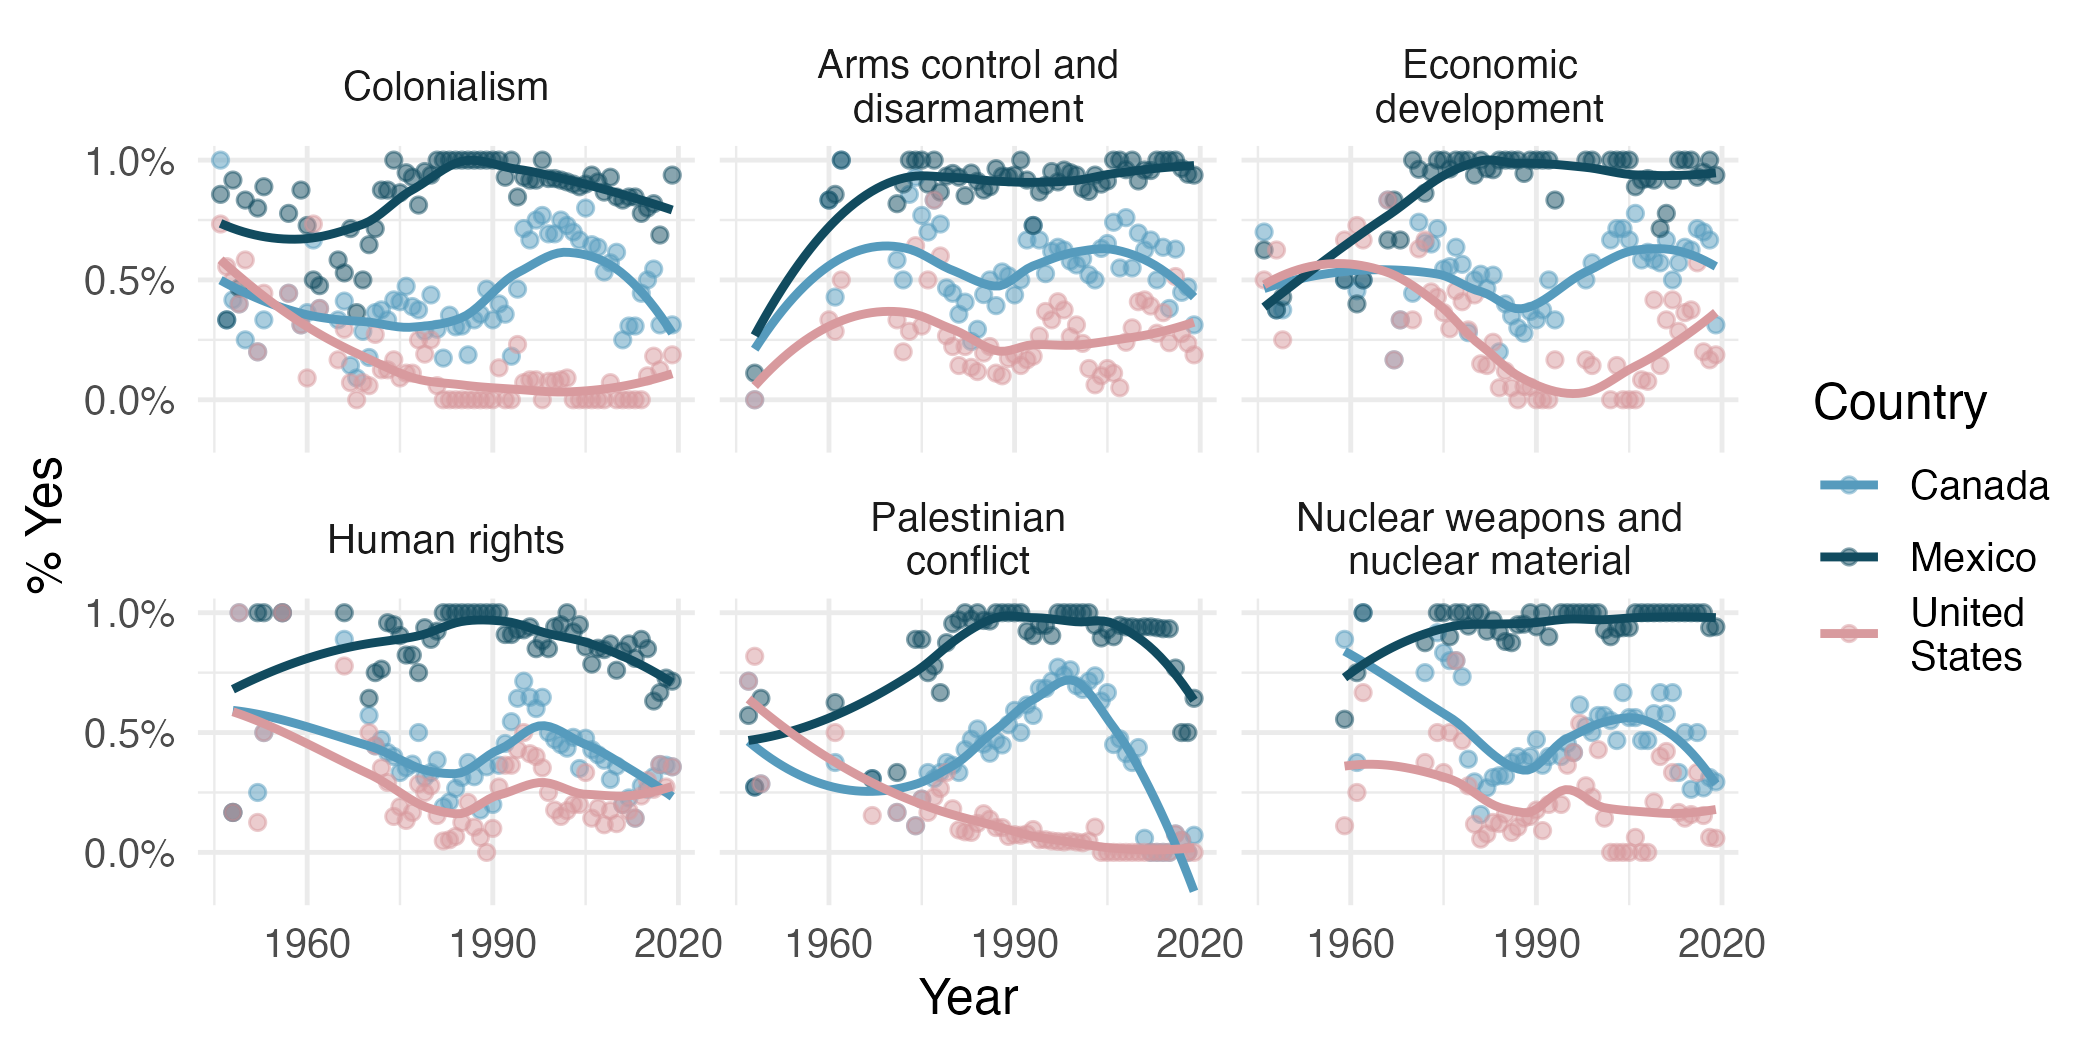
\includegraphics[width=1\textwidth,height=\textheight]{01-data-hello_files/figure-pdf/unnamed-chunk-33-1.png}

  \vspace{-5mm}

  \begin{enumerate}
  \def\labelenumii{\alph{enumii}.}
  \item
    List the variables used in creating this visualization.
  \item
    Indicate whether each variable is numerical or categorical. If
    numerical, identify as continuous or discrete. If categorical,
    indicate if the variable is ordinal.
  \end{enumerate}
\end{enumerate}

\clearpage

\begin{enumerate}
\def\labelenumi{\arabic{enumi}.}
\setcounter{enumi}{14}
\item
  \textbf{UK baby names.} The visualization below shows the number of
  baby girls born in the United Kingdom (comprised of England \& Wales,
  Northern Ireland, and Scotland) who were given the name ``Fiona'' over
  the years.\footnote{The
    \href{https://mine-cetinkaya-rundel.github.io/ukbabynames/reference/ukbabynames.html}{\texttt{ukbabynames}}
    data used in this exercise can be found in the
    \href{https://mine-cetinkaya-rundel.github.io/ukbabynames/}{\textbf{ukbabynames}}
    R package.}

  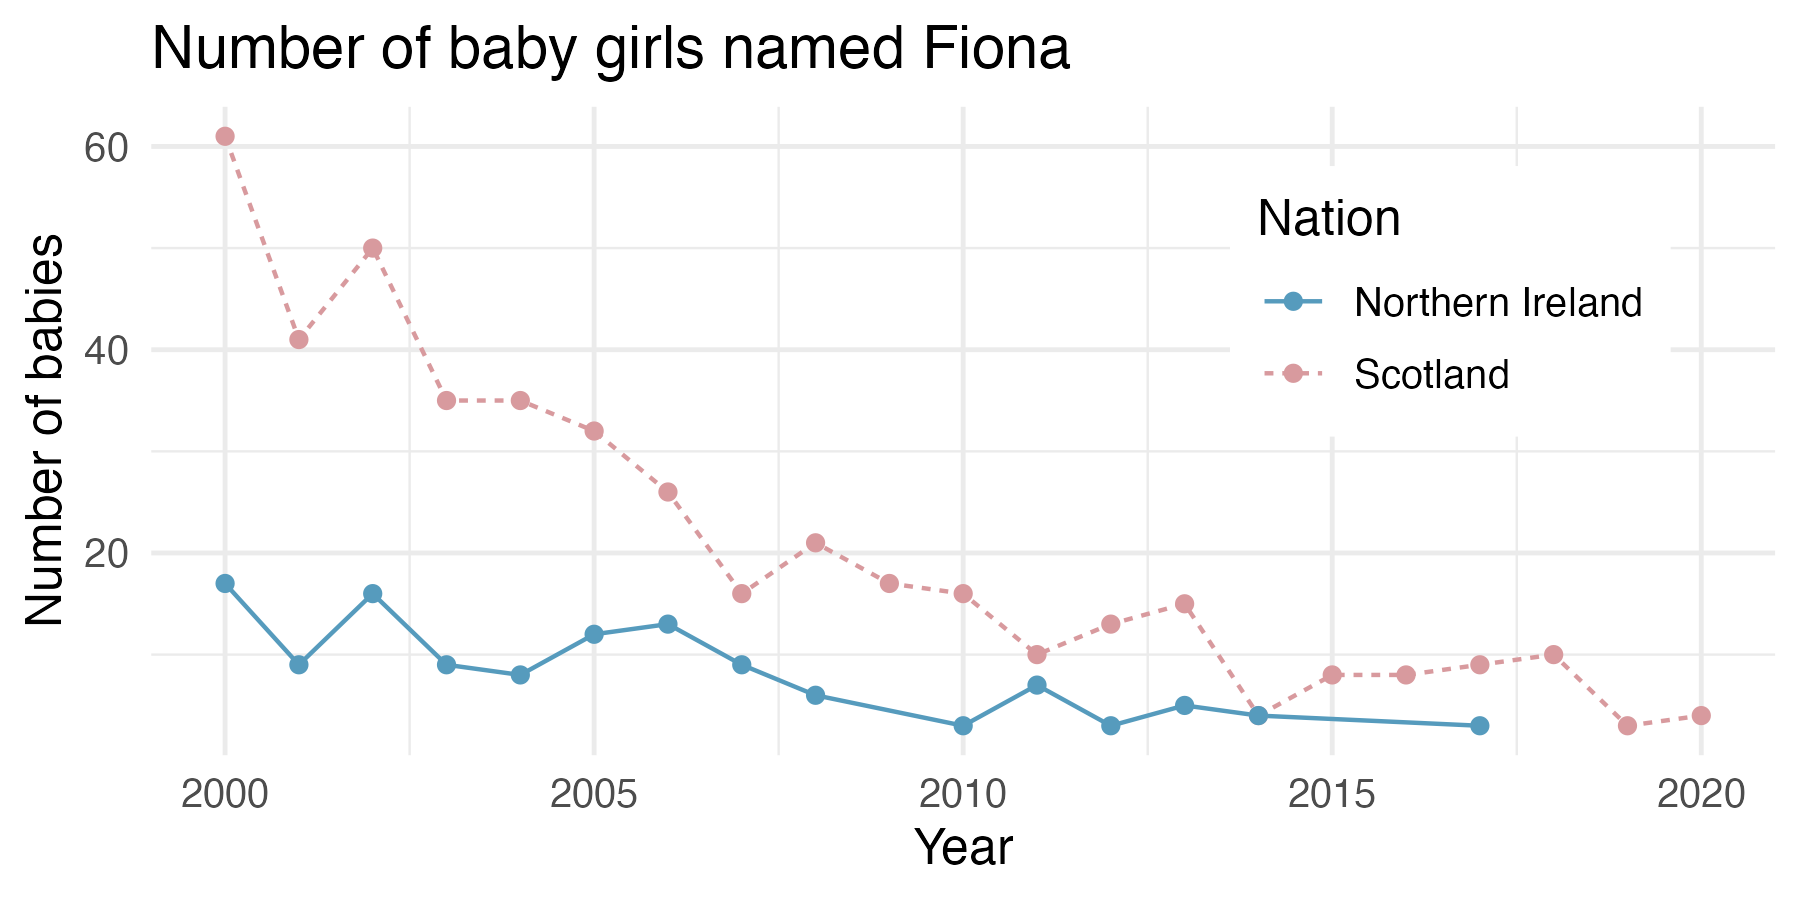
\includegraphics[width=0.8\textwidth,height=\textheight]{01-data-hello_files/figure-pdf/unnamed-chunk-34-1.png}

  \begin{enumerate}
  \def\labelenumii{\alph{enumii}.}
  \item
    List the variables you believe were necessary to create this
    visualization.
  \item
    Indicate whether each variable is numerical or categorical. If
    numerical, identify as continuous or discrete. If categorical,
    indicate if the variable is ordinal.
  \end{enumerate}
\item
  \textbf{Shows on Netflix.} The visualization below shows the
  distribution of ratings of TV shows on Netflix (a streaming
  entertainment service) based on the decade they were released in and
  the country they were produced in. In the dataset, each observation is
  a TV show.\footnote{The
    \href{https://github.com/rfordatascience/tidytuesday/blob/master/data/2021/2021-04-20/readme.md}{\texttt{netflix\_titles}}
    data used in this exercise can be found in the
    \href{https://cran.r-project.org/web/packages/tidytuesdayR/index.html}{\textbf{tidytuesdayR}}
    R package.}

  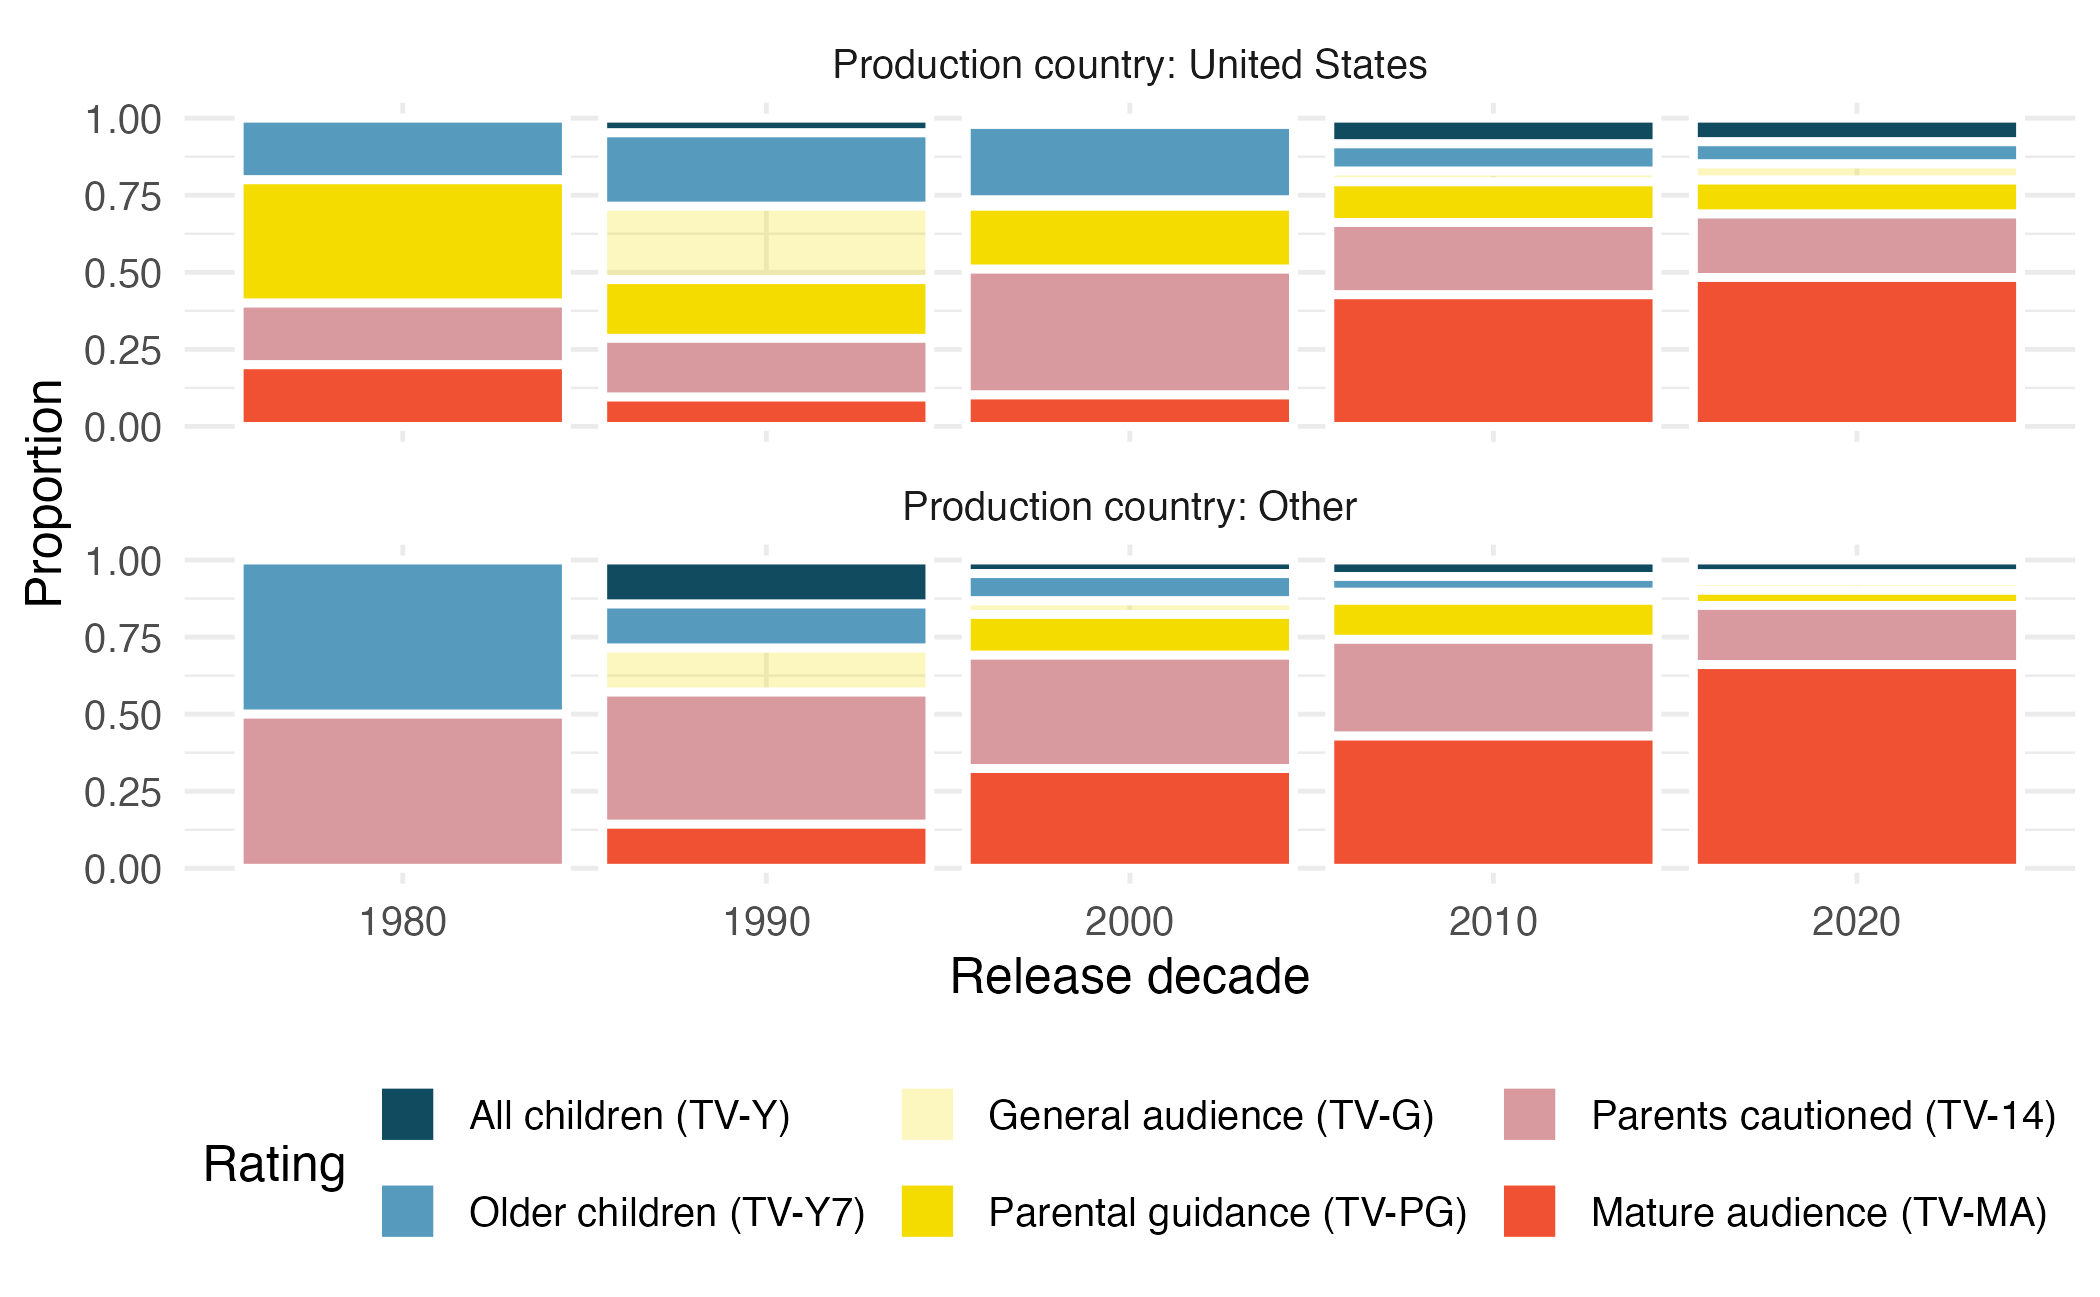
\includegraphics[width=0.9\textwidth,height=\textheight]{01-data-hello_files/figure-pdf/unnamed-chunk-35-1.png}

  \begin{enumerate}
  \def\labelenumii{\alph{enumii}.}
  \item
    List the variables you believe were necessary to create this
    visualization.
  \item
    Indicate whether each variable is numerical or categorical. If
    numerical, identify as continuous or discrete. If categorical,
    indicate if the variable is ordinal.
  \end{enumerate}
\end{enumerate}

\clearpage

\begin{enumerate}
\def\labelenumi{\arabic{enumi}.}
\setcounter{enumi}{16}
\item
  \textbf{Stanford Open Policing.} The Stanford Open Policing project
  gathers, analyzes, and releases records from traffic stops by law
  enforcement agencies across the United States. Their goal is to help
  researchers, journalists, and policy makers investigate and improve
  interactions between police and the public. The following is an
  excerpt from a summary table created based off of the data collected
  as part of this project. (Pierson et al. 2020)

  \begin{table}[H]
  \centering
  \begin{tabular}[t]{lllccc}
  \toprule
  \multicolumn{2}{c}{ } & \multicolumn{2}{c}{Driver} & \multicolumn{2}{c}{Car} \\
  \cmidrule(l{3pt}r{3pt}){3-4} \cmidrule(l{3pt}r{3pt}){5-6}
  County & State & Race / Ethnicity & Arrest rate & Stops / year & Search rate\\
  \midrule
  Apache County & AZ & Black & 0.016 & 266 & 0.077\\
  Apache County & AZ & Hispanic & 0.018 & 1008 & 0.053\\
  Apache County & AZ & White & 0.006 & 6322 & 0.017\\
  Cochise County & AZ & Black & 0.015 & 1169 & 0.047\\
  ... & ... & ... & ... & ... & ...\\
  Wood County & WI & Hispanic & 0.029 & 27 & 0.036\\
  Wood County & WI & White & 0.029 & 1157 & 0.033\\
  \bottomrule
  \end{tabular}
  \end{table}

  \begin{enumerate}
  \def\labelenumii{\alph{enumii}.}
  \item
    What variables were collected on each individual traffic stop in
    order to create the summary table above?
  \item
    State whether each variable is numerical or categorical. If
    numerical, state whether it is continuous or discrete. If
    categorical, state whether it is ordinal or not.
  \item
    Suppose we wanted to evaluate whether vehicle search rates are
    different for drivers of different races. In this analysis, which
    variable would be the response variable and which variable would be
    the explanatory variable?
  \end{enumerate}
\end{enumerate}

\vspace{10mm}

\begin{enumerate}
\def\labelenumi{\arabic{enumi}.}
\setcounter{enumi}{17}
\item
  \textbf{Space launches.} The following summary table shows the number
  of space launches in the US by the type of launching agency and the
  outcome of the launch (success or failure).\footnote{The data used in
    this exercise comes from the
    \href{https://www.openintro.org/go?id=textbook-space-launches-data&referrer=ims0_html}{JSR
    Launch Vehicle Database, 2019 Feb 10 Edition}.}

  \begin{table}[H]
  \centering
  \begin{tabular}[t]{lrrrr}
  \toprule
  \multicolumn{1}{c}{ } & \multicolumn{2}{c}{1957 - 1999} & \multicolumn{2}{c}{2000-2018} \\
  \cmidrule(l{3pt}r{3pt}){2-3} \cmidrule(l{3pt}r{3pt}){4-5}
   & Failure & Success & Failure & Success\\
  \midrule
  Private & 13 & 295 & 10 & 562\\
  State & 281 & 3751 & 33 & 711\\
  Startup & 0 & 0 & 5 & 65\\
  \bottomrule
  \end{tabular}
  \end{table}

  \begin{enumerate}
  \def\labelenumii{\alph{enumii}.}
  \item
    What variables were collected on each launch in order to create to
    the summary table above?
  \item
    State whether each variable is numerical or categorical. If
    numerical, state whether it is continuous or discrete. If
    categorical, state whether it is ordinal or not.
  \item
    Suppose we wanted to study how the success rate of launches vary
    between launching agencies and over time. In this analysis, which
    variable would be the response variable and which variable would be
    the explanatory variable?
  \end{enumerate}
\end{enumerate}

\clearpage

\begin{enumerate}
\def\labelenumi{\arabic{enumi}.}
\setcounter{enumi}{18}
\item
  \textbf{Pet names.} The city of Seattle, WA has an open data portal
  that includes pets registered in the city. For each registered pet, we
  have information on the pet's name and species. The following
  visualization plots the proportion of dogs with a given name versus
  the proportion of cats with the same name. The 20 most common cat and
  dog names are displayed. The diagonal line on the plot is the
  \(x = y\) line; if a name appeared on this line, the name's popularity
  would be exactly the same for dogs and cats.\footnote{The
    \href{http://openintrostat.github.io/openintro/reference/seattlepets.html}{\texttt{seattlepets}}
    data used in this exercise can be found in the
    \href{http://openintrostat.github.io/openintro}{\textbf{openintro}}
    R package.}

  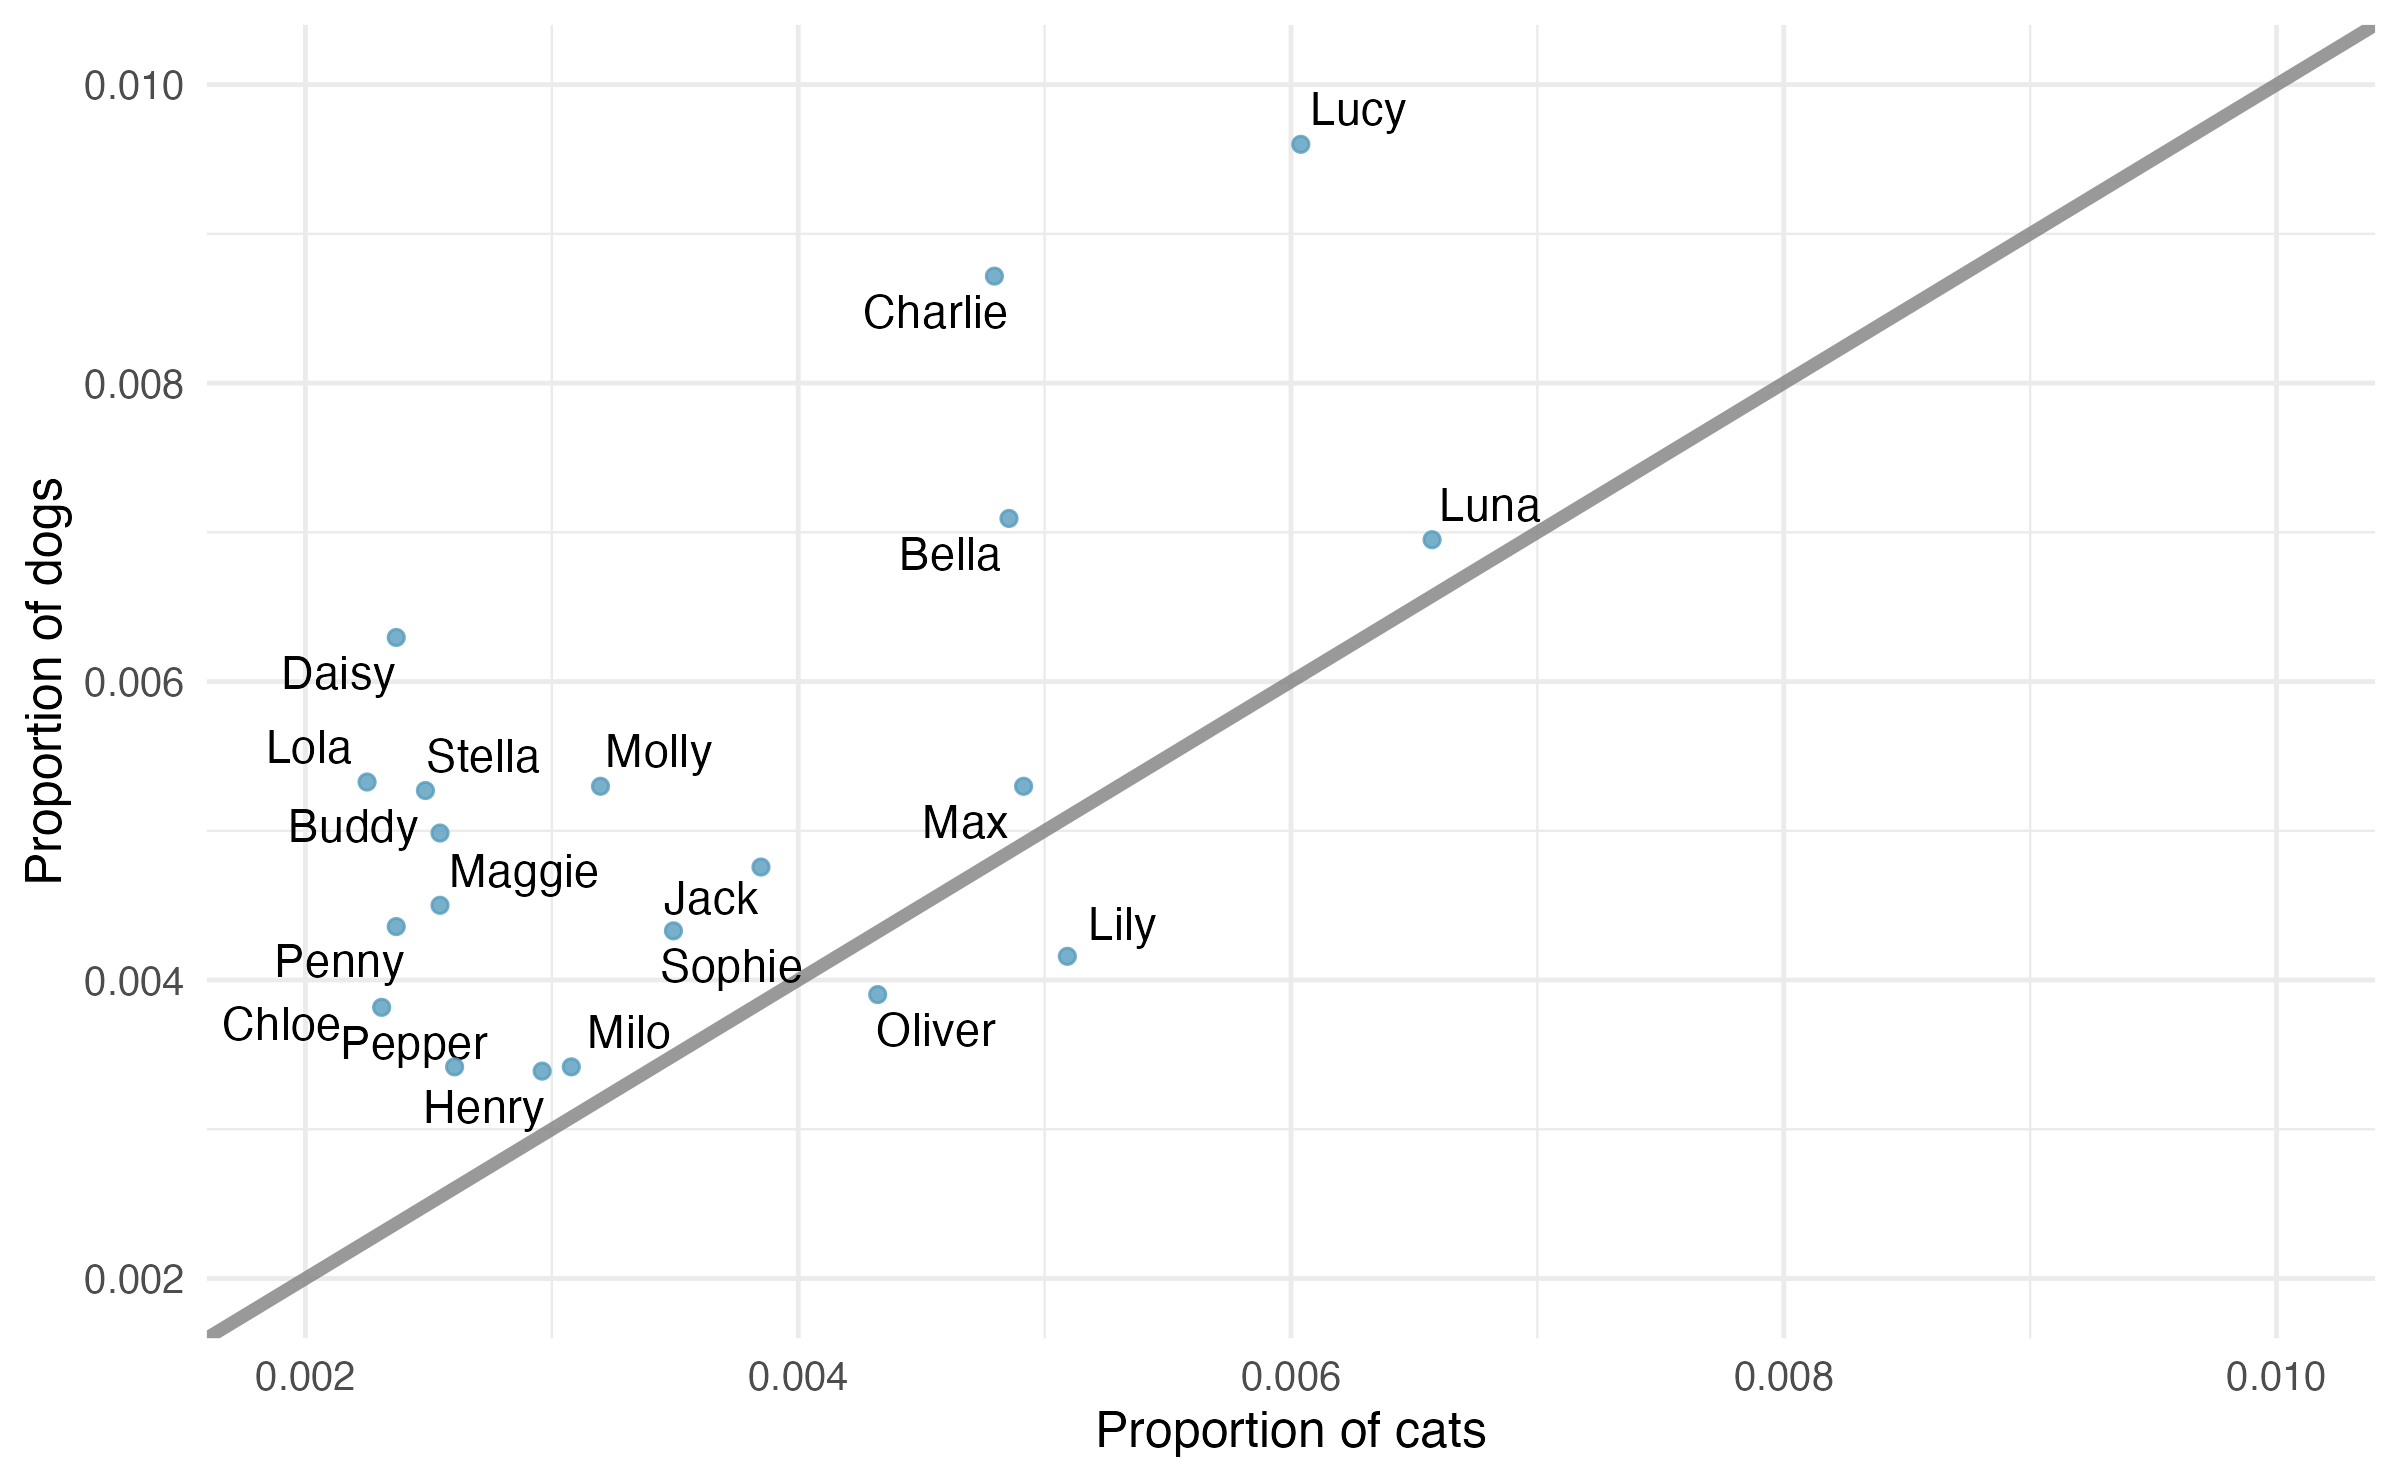
\includegraphics[width=0.8\textwidth,height=\textheight]{01-data-hello_files/figure-pdf/unnamed-chunk-38-1.png}

  \begin{enumerate}
  \def\labelenumii{\alph{enumii}.}
  \item
    Are these data collected as part of an experiment or an
    observational study?
  \item
    What is the most common dog name? What is the most common cat name?
  \item
    What names are more common for cats than dogs?
  \item
    Is the relationship between the two variables positive or negative?
    What does this mean in context of the data?
  \end{enumerate}
\item
  \textbf{Stressed out in an elevator.} In a study evaluating the
  relationship between stress and muscle cramps, half the subjects are
  randomly assigned to be exposed to increased stress by being placed
  into an elevator that falls rapidly and stops abruptly and the other
  half are left at no or baseline stress.

  \begin{enumerate}
  \def\labelenumii{\alph{enumii}.}
  \item
    What type of study is this?
  \item
    Can this study be used to conclude a causal relationship between
    increased stress and muscle cramps?
  \end{enumerate}
\end{enumerate}

\end{exercises}

\chapter{Study design}\label{sec-data-design}

\begin{chapterintro}
Before digging into the details of working with data, we stop to think
about how data come to be. That is, if the data are to be used to make
broad and complete conclusions, then it is important to understand who
or what the data represent. One important aspect of data provenance is
sampling. Knowing how the observational units were selected from a
larger entity will allow for generalizations back to the population from
which the data were randomly selected. Additionally, by understanding
the structure of the study, causal relationships can be separated from
those relationships which are only associated. A good question to ask
oneself before working with the data at all is, ``How were these
observations collected?''. You will learn a lot about the data by
understanding its source.

\end{chapterintro}

\vspace{-5mm}

\section{Sampling principles and
strategies}\label{sec-sampling-principles-strategies}

The first step in conducting research is to identify topics or questions
that are to be investigated. A clearly laid out research question is
helpful in identifying what subjects or cases should be studied and what
variables are important. It is also important to consider \emph{how}
data are collected so that the data are reliable and help achieve the
research goals.

\subsection{Populations and samples}\label{populations-and-samples}

Consider the following three research questions:

\begin{enumerate}
\def\labelenumi{\arabic{enumi}.}
\tightlist
\item
  What is the average mercury content in swordfish in the Atlantic
  Ocean?
\item
  Over the last five years, what is the average time to complete a
  degree for Duke undergrads?
\item
  Does a new drug reduce the number of deaths in patients with severe
  heart disease?
\end{enumerate}

Each research question refers to a target \textbf{population}. In the
first question, the target population is all swordfish in the Atlantic
Ocean, and each fish represents a case. Oftentimes, it is not feasible
to collect data for every case in a population. Collecting data for an
entire population is called a \textbf{census}. A census is difficult
because it is too expensive to collect data for the entire population,
but it might also be because it is difficult or impossible to identify
the entire population of interest! Instead, a sample is taken. A
\textbf{sample} is the data you have. Ideally, a sample is a small
fraction of the population. For instance, 60 swordfish (or some other
number) in the population might be selected, and this sample data may be
used to provide an estimate of the population average and to answer the
research question.

\begin{guidedpractice}
For the second and third questions above, identify the target population
and what represents an individual case.\footnote{The question
  \emph{``Over the last five years, what is the average time to complete
  a degree for Duke undergrads?''} is only relevant to students who
  complete their degree; the average cannot be computed using a student
  who never finished their degree. Thus, only Duke undergrads who
  graduated in the last five years represent cases in the population
  under consideration. Each such student is an individual case. For the
  question \emph{``Does a new drug reduce the number of deaths in
  patients with severe heart disease?''}, a person with severe heart
  disease represents a case. The population includes all people with
  severe heart disease.}

\end{guidedpractice}

\vspace{-5mm}

\subsection{Parameters and statistics}\label{parameters-and-statistics}

In most statistical analysis procedures, the research question at hand
boils down to understanding a numerical summary. The number (or set of
numbers) may be a quantity you are already familiar with (like the
average) or it may be something you learn through this text (like the
slope and intercept from a least squares model, provided in
Section~\ref{sec-least-squares-regression}).

A numerical summary can be calculated on either the sample of
observations or the entire population. However, measuring every unit in
the population is usually prohibitive. So, a ``typical'' numerical
summary is calculated from a sample. Yet, we can still conceptualize
calculating the average income of all adults in Argentina.

We use specific terms in order to differentiate when a number is being
calculated on a sample of data (\textbf{sample statistic}) and when it
is being calculated or considered for calculation on the entire
population (\textbf{population parameter}). The terms statistic and
parameter are useful for communicating claims and models and will be
used extensively in later chapters which delve into making inference on
populations.

\index{sample statistic} \index{population parameter}

\subsection{Anecdotal evidence}\label{anecdotal-evidence}

\index{bias}

Consider the following possible responses to the three research
questions:

\begin{enumerate}
\def\labelenumi{\arabic{enumi}.}
\tightlist
\item
  A man on the news got mercury poisoning from eating swordfish, so the
  average mercury concentration in swordfish must be dangerously high.
\item
  I met two students who took more than 7 years to graduate from Duke,
  so it must take longer to graduate at Duke than at many other
  colleges.
\item
  My friend's dad had a heart attack and died after they gave him a new
  heart disease drug, so the drug must not work.
\end{enumerate}

Each conclusion is based on data. However, there are two problems.
First, the data only represent one or two cases. Second, and more
importantly, it is unclear whether these cases are actually
representative of the population. Data collected in this haphazard
fashion are called \textbf{anecdotal
evidence}\index{anecdotal evidence}.

\begin{important}
\textbf{Anecdotal evidence.}

Be careful of data collected in a haphazard fashion. Such evidence may
be true and verifiable, but it may only represent extraordinary cases
and therefore not be a good representation of the population.

\end{important}

Anecdotal evidence typically is composed of unusual cases that we recall
based on their striking characteristics. For instance, we are more
likely to remember the two people we met who took 7 years to graduate
than the six others who graduated in four years. Instead, of looking at
the most unusual cases, we should examine a sample of many cases that
better represent the population.

\subsection{Sampling from a
population}\label{sampling-from-a-population}

\index{sampling!random} \index{bias}

We might try to estimate the time to graduation for Duke undergraduates
in the last five years by collecting a sample of graduates. All
graduates in the last five years represent the
\emph{population}\index{population}, and graduates who are selected for
review are collectively called the \emph{sample}\index{sample}. In
general, we always seek to \emph{randomly} select a sample from a
population. The most basic type of random selection is equivalent to how
raffles are conducted. For example, in selecting graduates, we could
write each graduate's name on a raffle ticket and draw 10 tickets. The
selected names would represent a random sample of 10 graduates.

\vspace{-2mm}

\begin{figure}[H]

\centering{

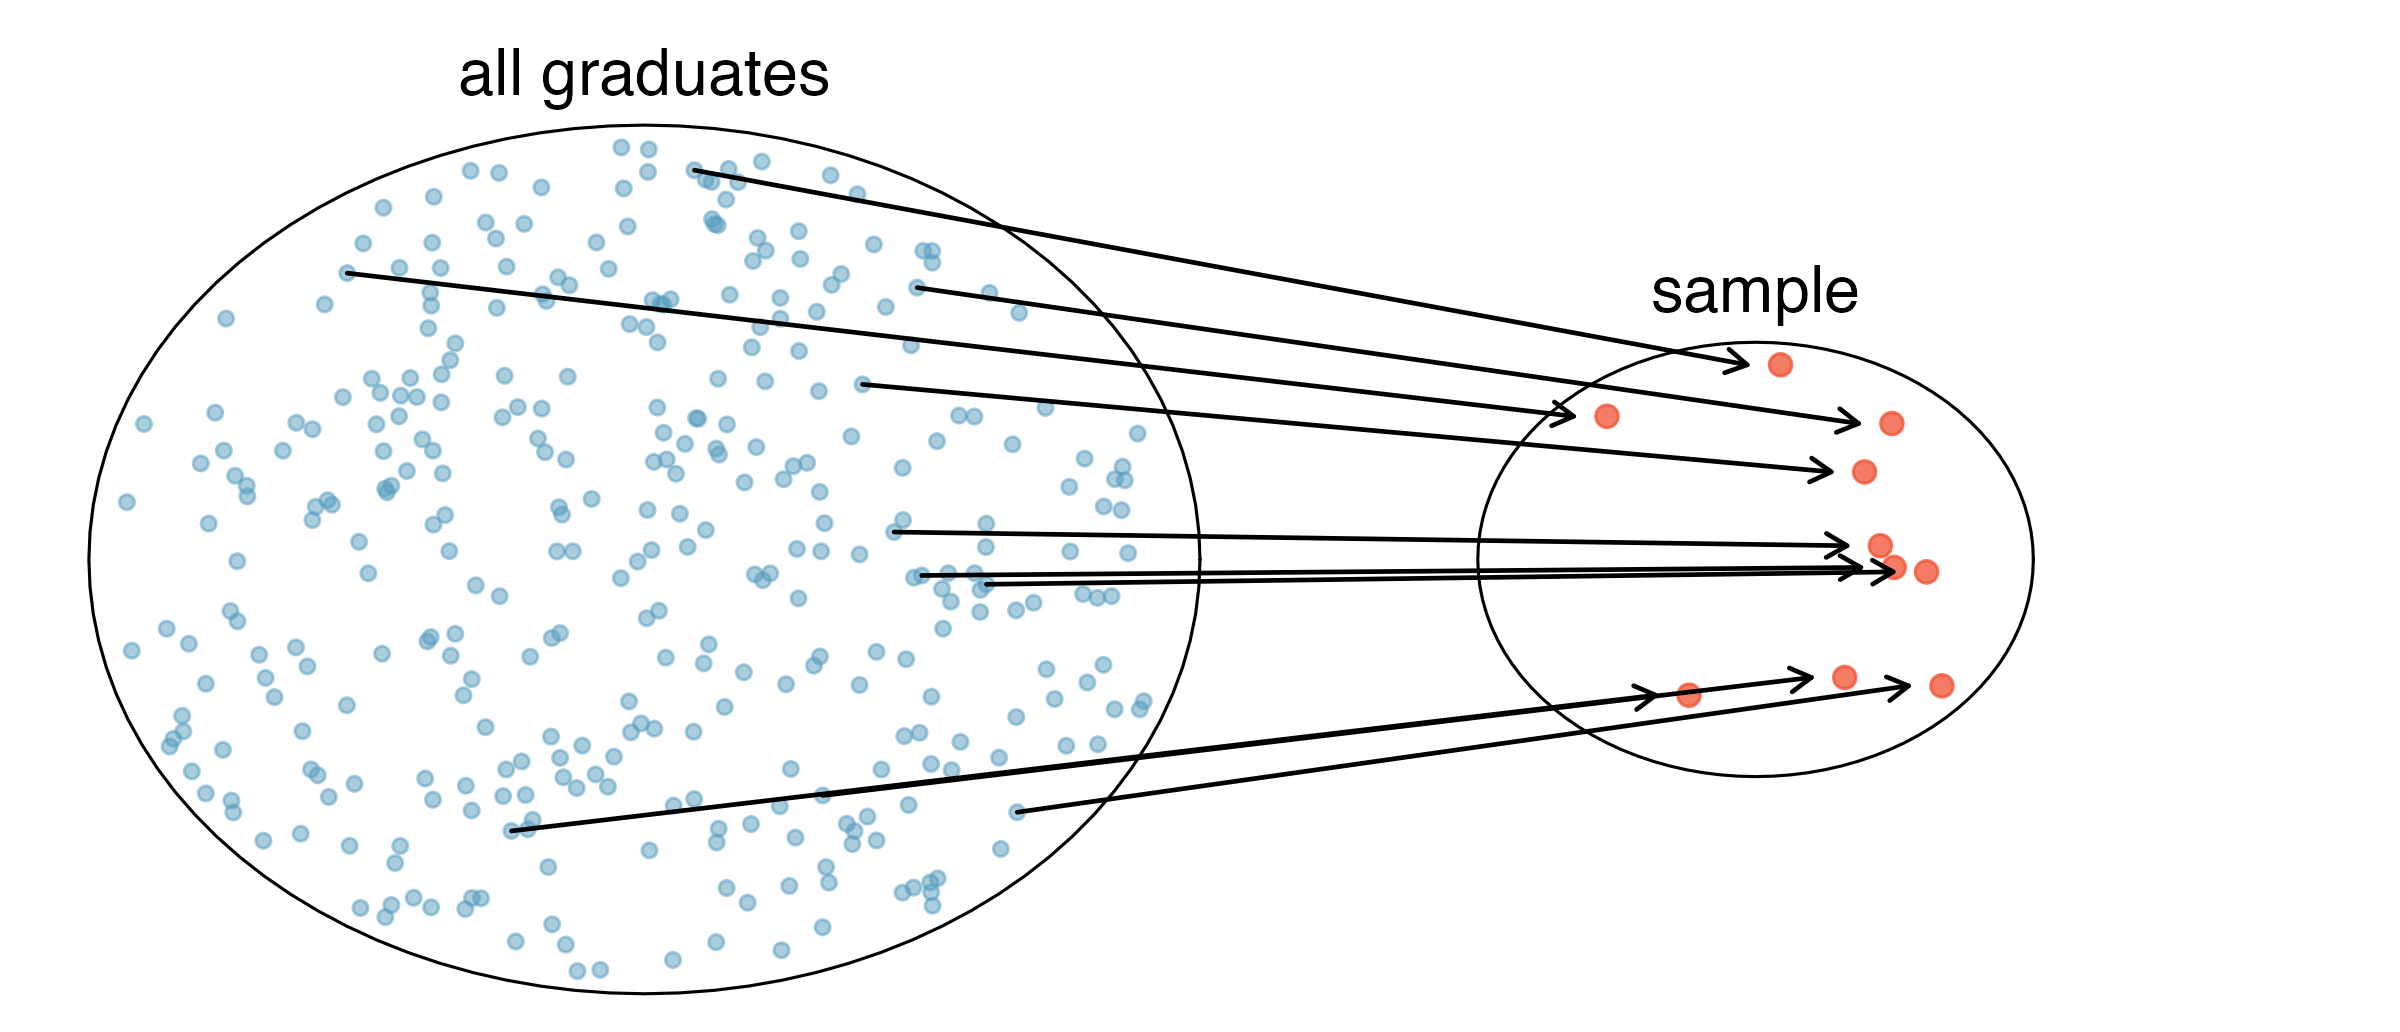
\includegraphics[width=0.7\textwidth,height=\textheight]{02-data-design_files/figure-pdf/fig-pop-to-sample-1.png}

}

\caption{\label{fig-pop-to-sample}10 graduates are randomly selected
from the population to be included in the sample.}

\end{figure}%

\vspace{-3mm}

\begin{workedexample}
Suppose we ask a student who happens to be majoring in nutrition to
select several graduates for the study. Which students do you think they
might pick? Do you think their sample would be representative of all
graduates?

\begin{center}\rule{0.5\linewidth}{0.5pt}\end{center}

They might pick a disproportionate number of graduates from
health-related fields, as shown in
Figure~\ref{fig-pop-to-sub-sample-graduates}. When selecting samples by
hand, we run the risk of picking a \textbf{biased} sample, even if our
bias is unintended.

\end{workedexample}

\vspace{-3mm}

\begin{figure}[H]

\centering{

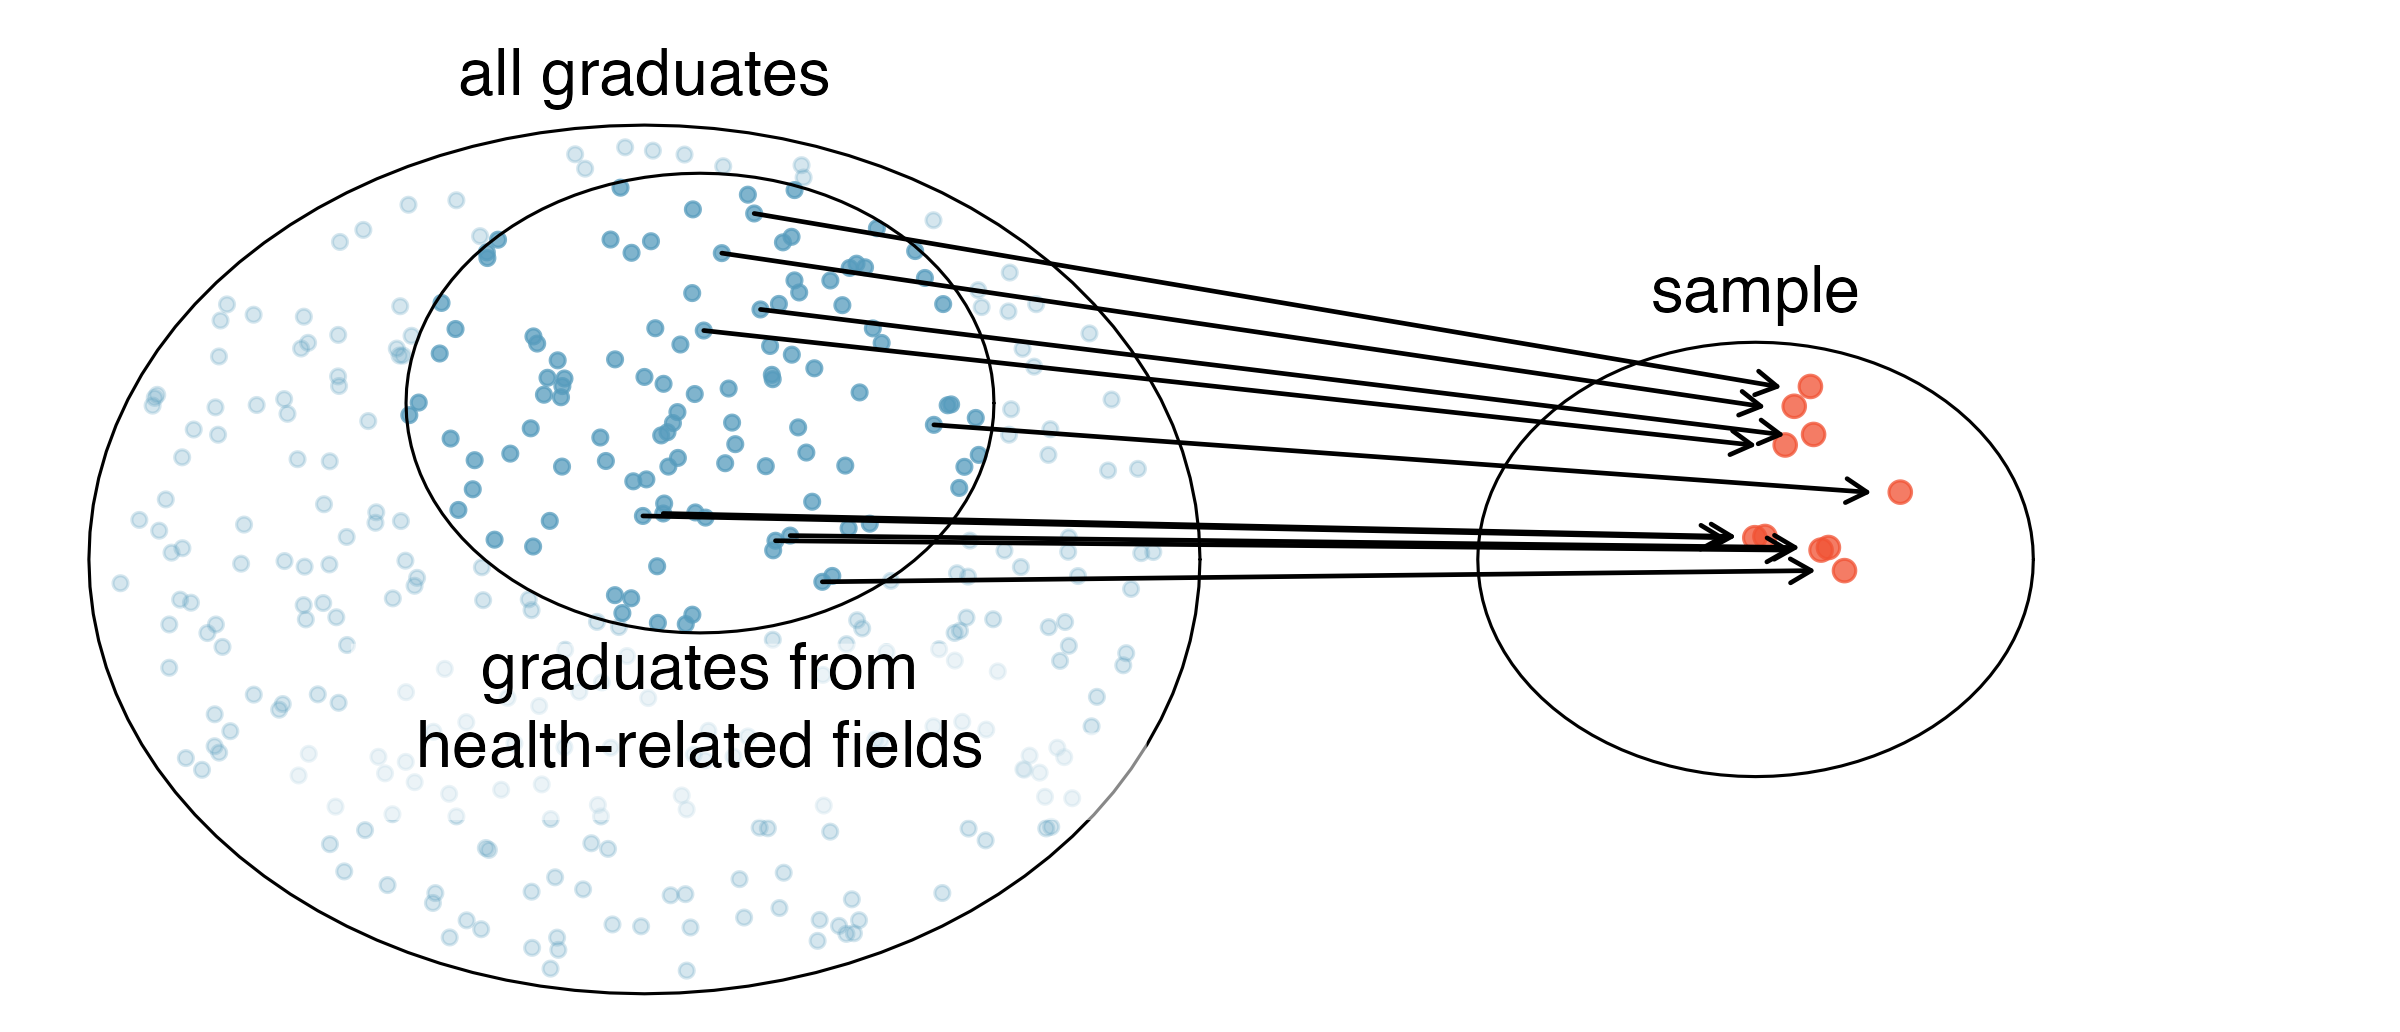
\includegraphics[width=0.7\textwidth,height=\textheight]{02-data-design_files/figure-pdf/fig-pop-to-sub-sample-graduates-1.png}

}

\caption{\label{fig-pop-to-sub-sample-graduates}Asked to pick a sample
of graduates, a nutrition major might inadvertently pick a
disproportionate number of graduates from health-related majors.}

\end{figure}%

\clearpage

If someone was permitted to pick and choose exactly which graduates were
included in the sample, it is entirely possible that the sample would
overrepresent that person's interests, which may be entirely
unintentional. This introduces \textbf{bias} into a sample\index{bias}.
Sampling randomly helps address this problem. The most basic random
sample is called a \textbf{simple random
sample}\index{sampling!simple random} and is equivalent to drawing names
out of a hat to select cases. This means that each case in the
population has an equal chance of being included and the cases in the
sample are not related to each other.

The act of taking a simple random sample helps minimize bias. However,
bias can crop up in other ways. Even when people are picked at random,
e.g., for surveys, caution must be exercised if the \textbf{non-response
rate}\index{non-response rate} is high. For instance, if only 30\% of
the people randomly sampled for a survey actually respond, then it is
unclear whether the results are \textbf{representative} of the entire
population. This \textbf{non-response bias}\index{bias!non-response} can
skew results.

\begin{figure}[H]

\centering{

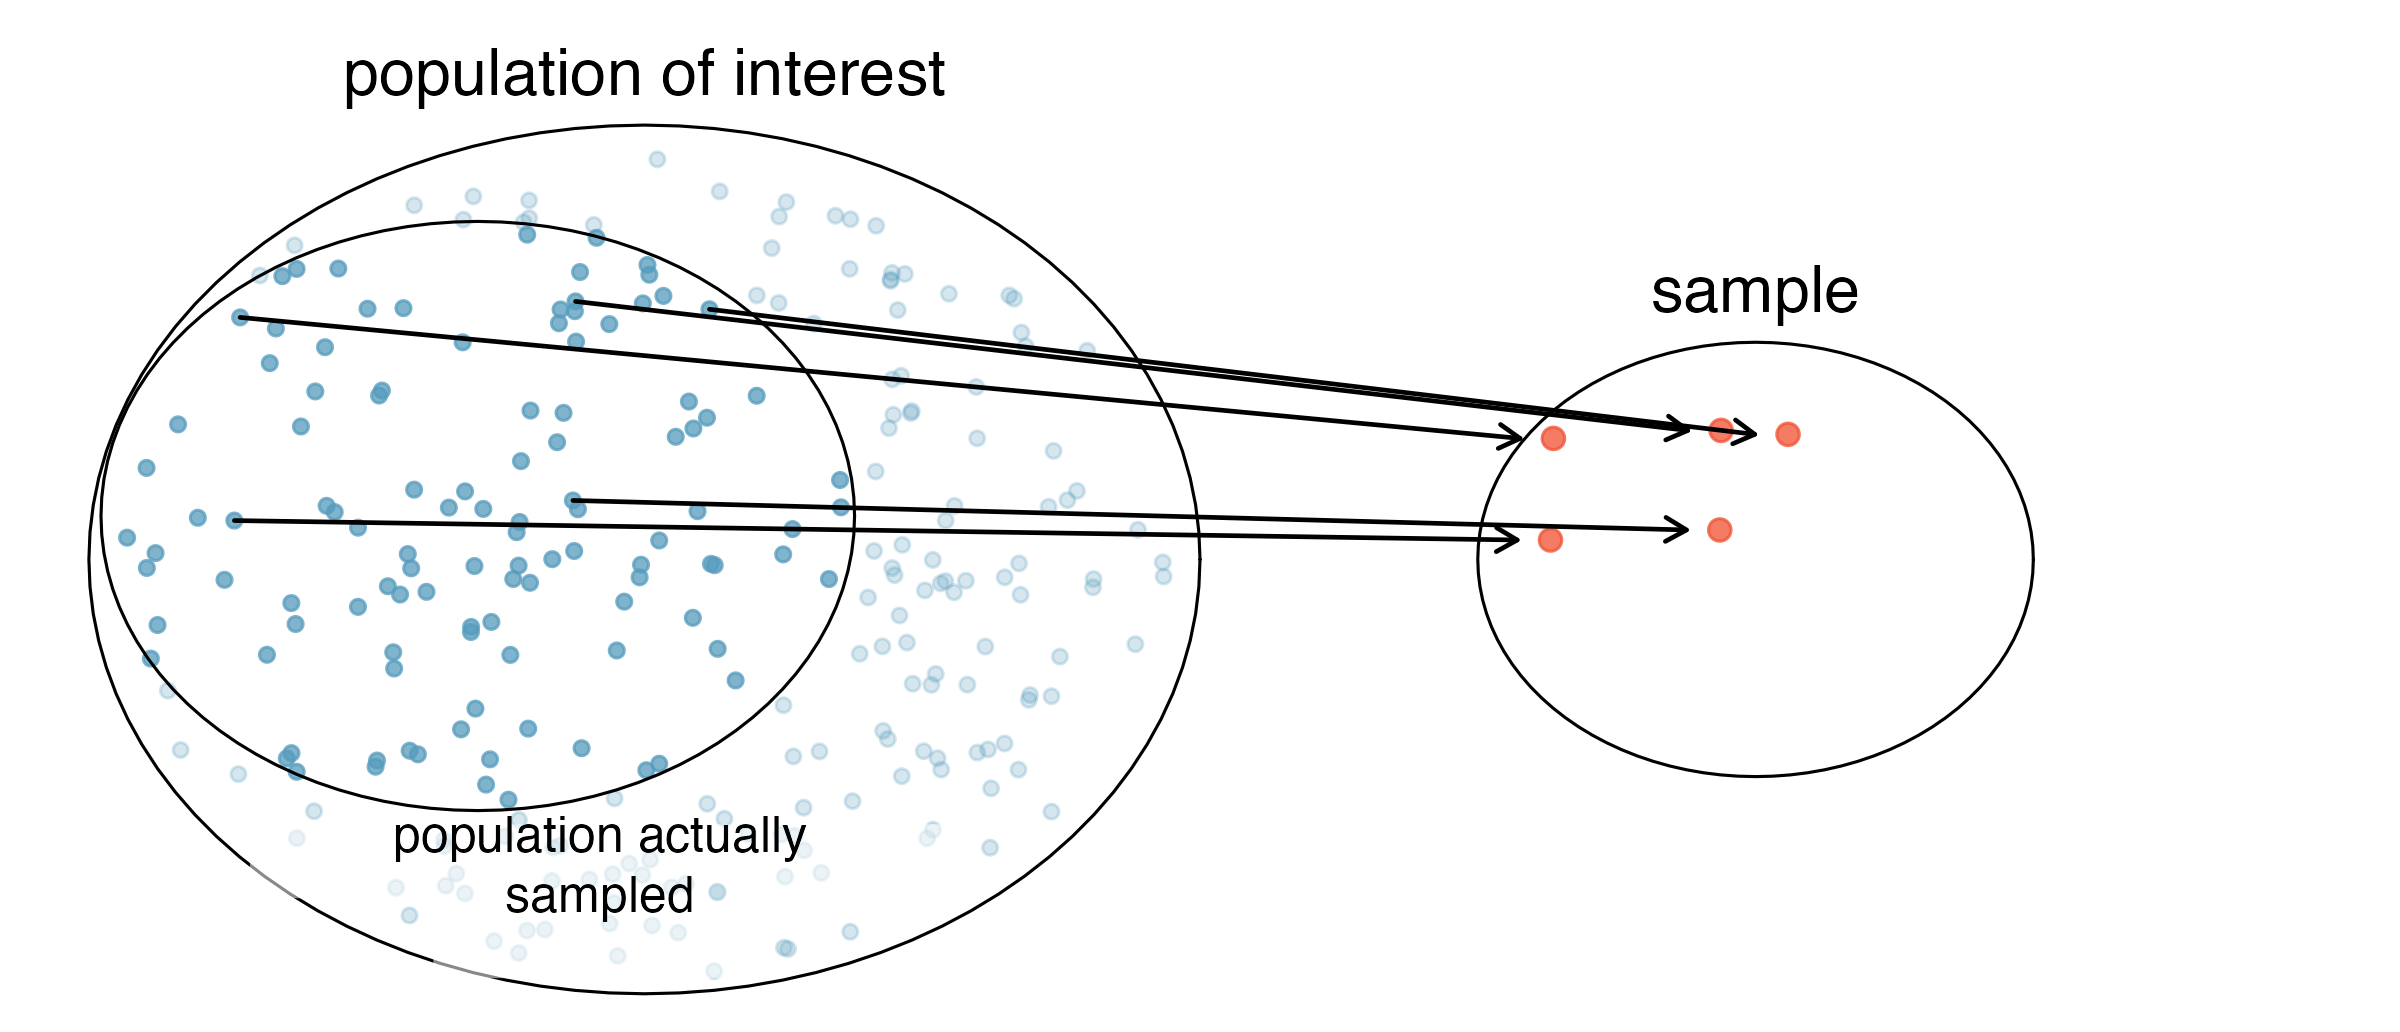
\includegraphics[width=0.7\textwidth,height=\textheight]{02-data-design_files/figure-pdf/fig-survey-sample-1.png}

}

\caption{\label{fig-survey-sample}Due to the possibility of
non-response, survey studies may only reach a certain group within the
population. It is difficult, and oftentimes impossible, to completely
fix this problem.}

\end{figure}%

Another common downfall is a \textbf{convenience
sample}\index{sampling!convenience}, where individuals who are easily
accessible are more likely to be included in the sample. For instance,
if a political survey is done by stopping people walking in the Bronx,
this will not represent all of New York City. It is often difficult to
discern what sub-population a convenience sample represents.

\begin{guidedpractice}
We can easily access ratings for products, sellers, and companies
through websites. These ratings are based only on those people who go
out of their way to provide a rating. If 50\% of online reviews for a
product are negative, do you think this means that 50\% of buyers are
dissatisfied with the product? Why?\footnote{Answers will vary. From our
  own anecdotal experiences, we believe people tend to rant more about
  products that fell below expectations than rave about those that
  perform as expected. For this reason, we suspect there is a negative
  bias in product ratings on sites like Amazon. However, since our
  experiences may not be representative, we also keep an open mind.}

\end{guidedpractice}

\index{sampling!random} \index{bias} \index{population} \index{sample}

\subsection{Four sampling methods}\label{sec-samp-methods}

Almost all statistical methods are based on the notion of implied
randomness. If data are not collected in a random framework from a
population, these statistical methods -- the estimates and errors
associated with the estimates -- are not reliable. Here we consider four
random sampling techniques: simple, stratified, cluster, and multistage
sampling. Figures Figure~\ref{fig-simple-stratified} and
Figure~\ref{fig-cluster-multistage} provide graphical representations of
these techniques.

\begin{figure}[H]

\centering{

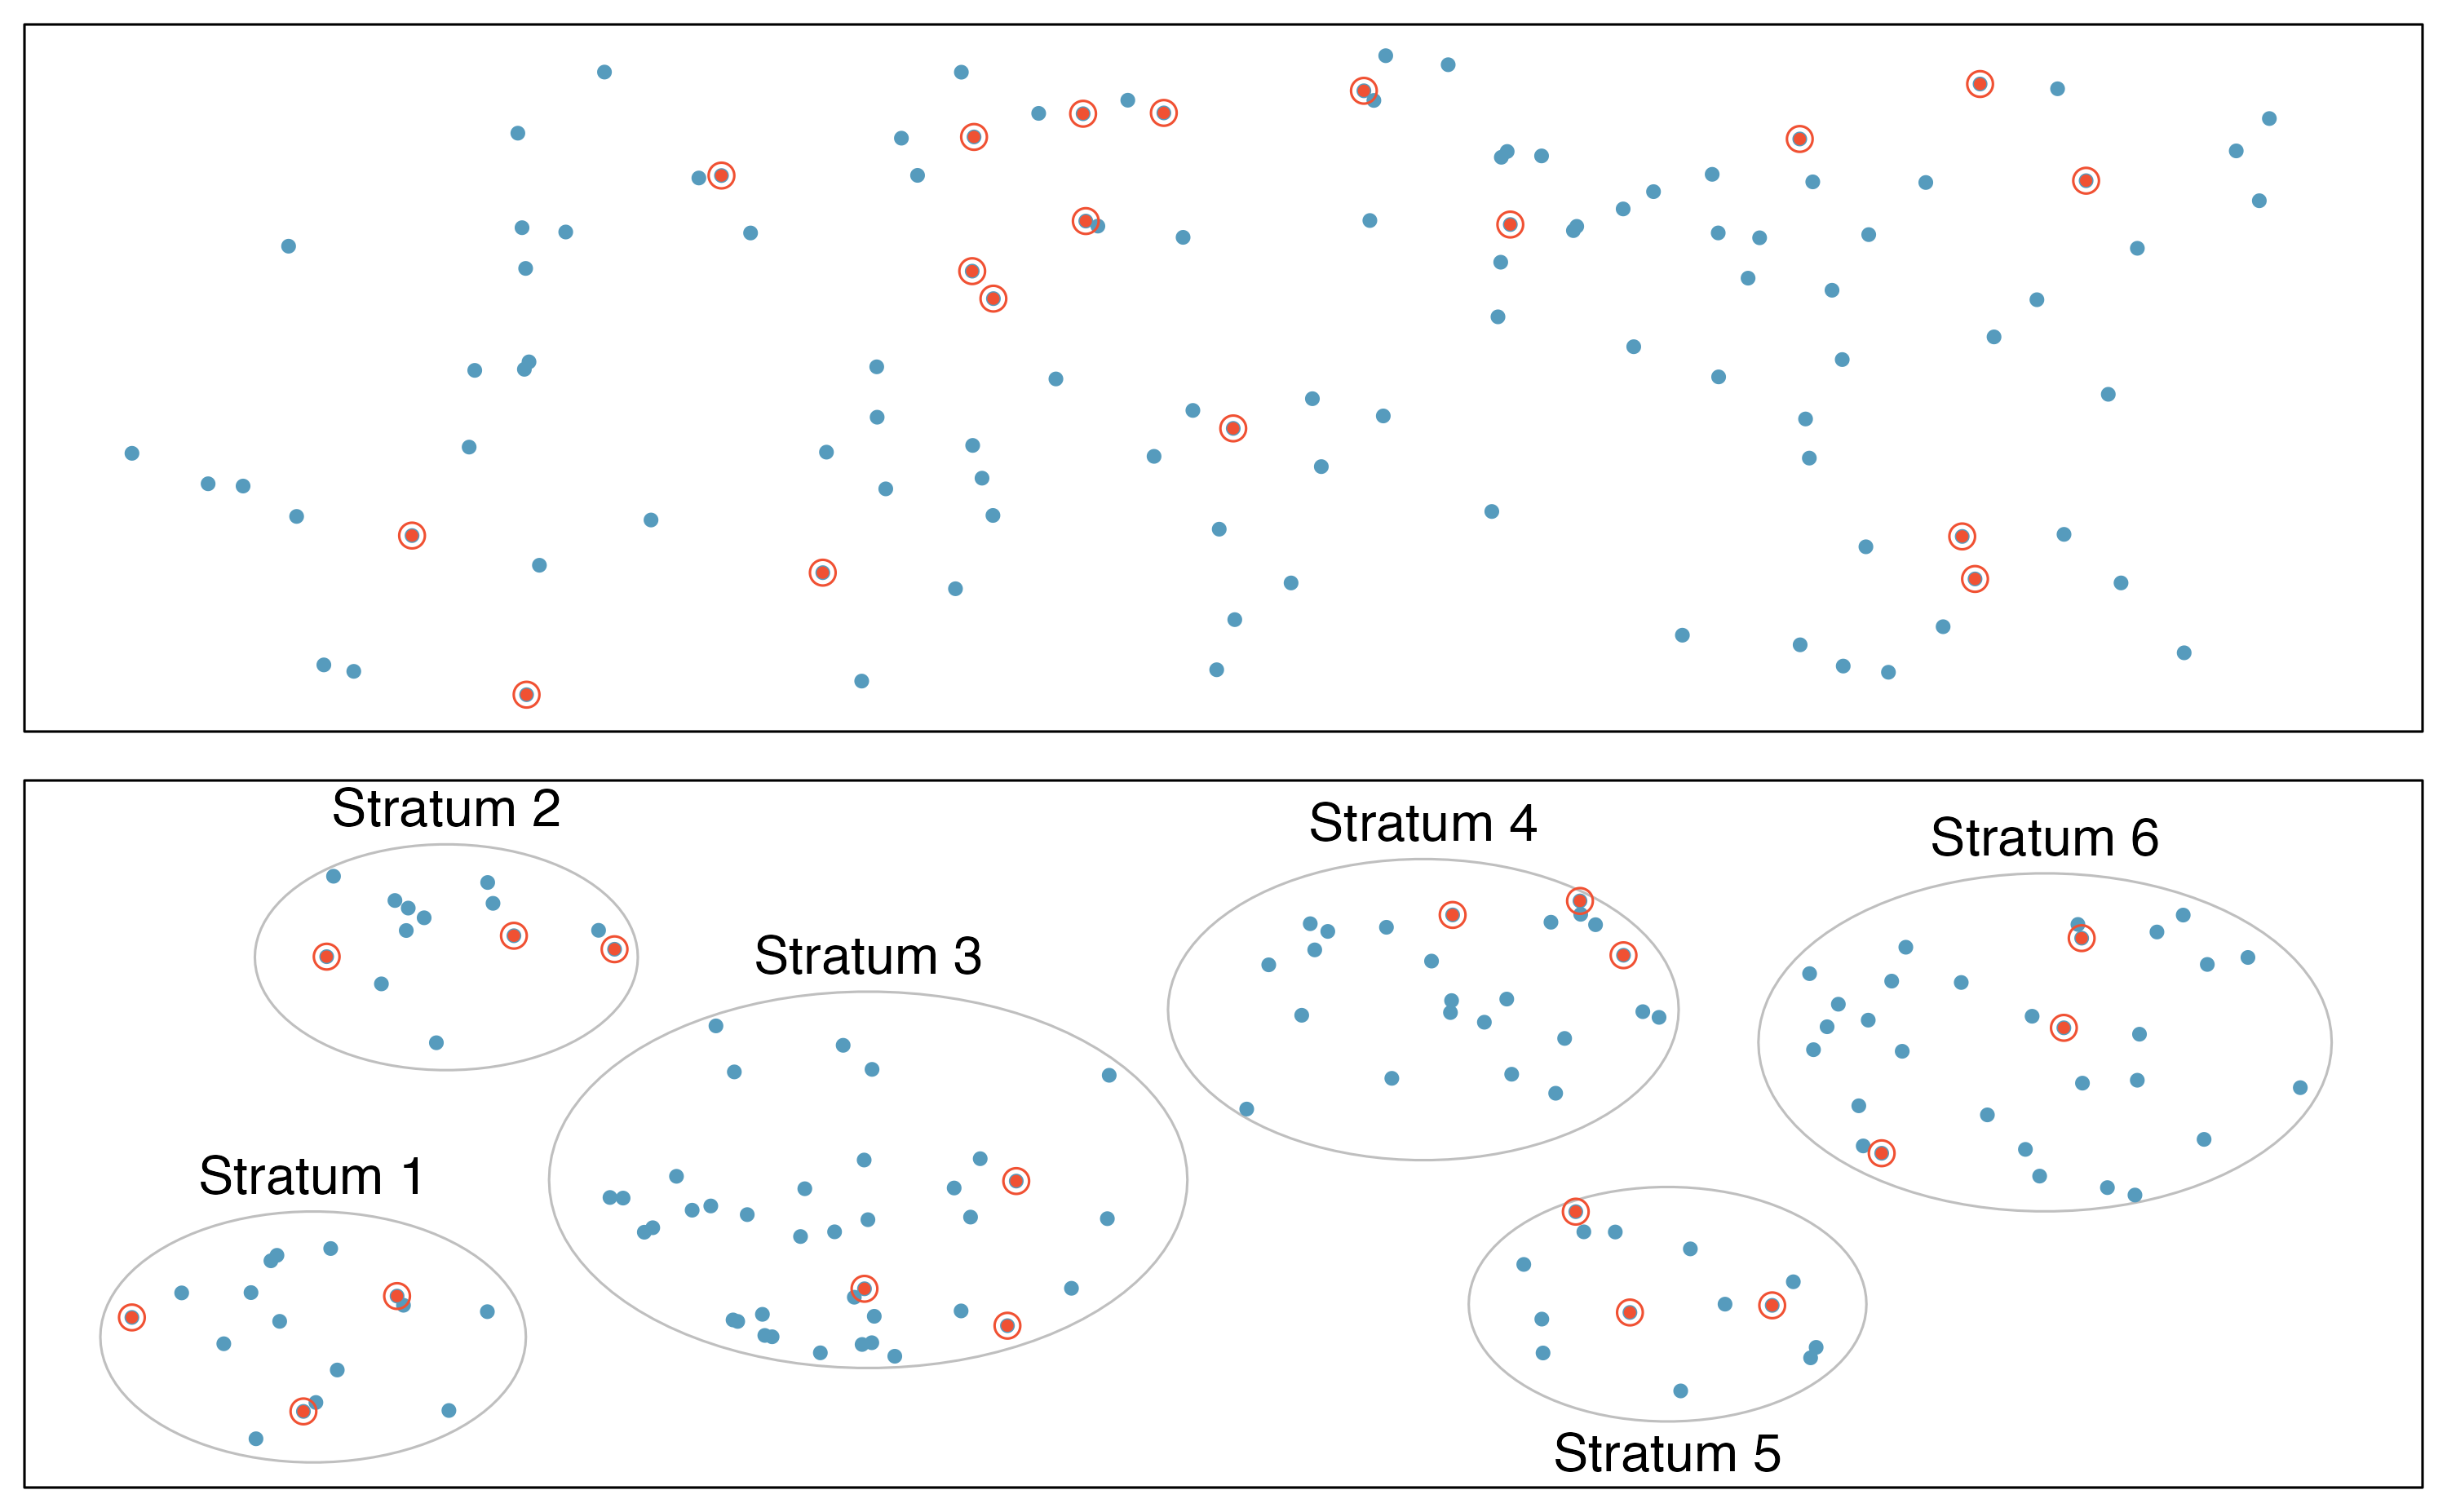
\includegraphics[width=0.8\textwidth,height=\textheight]{02-data-design_files/figure-pdf/fig-simple-stratified-1.png}

}

\caption{\label{fig-simple-stratified}Examples of simple random and
stratified sampling. In the top panel, simple random sampling was used
to randomly select the 18 cases (denoted in red). In the bottom panel,
stratified sampling was used: cases were first grouped into strata, then
simple random sampling was employed to randomly select 3 cases within
each stratum.'}

\end{figure}%

\textbf{Simple random sampling}\index{sampling!simple random} is
probably the most intuitive form of random sampling. Consider the
salaries of Major League Baseball (MLB) players, where each player is a
member of one of the league's 30 teams. To take a simple random sample
of 120 baseball players and their salaries, we could write the names of
that season's several hundreds of players onto slips of paper, drop the
slips into a bucket, shake the bucket around until we are sure the names
are all mixed up, then draw out slips until we have the sample of 120
players. In general, a sample is referred to as ``simple random'' if
each case in the population has an equal chance of being included in the
final sample \emph{and} knowing that a case is included in a sample does
not provide useful information about which other cases are included.

\textbf{Stratified sampling}\index{sampling!stratified} is a
divide-and-conquer sampling strategy. The population is divided into
groups called \textbf{strata}\index{sampling!strata}. The strata are
chosen so that similar cases are grouped together, then a second
sampling method, usually simple random sampling, is employed within each
stratum. In the baseball salary example, each of the 30 teams could
represent a stratum, since some teams have a lot more money (up to 4
times as much!). Then we might randomly sample 4 players from each team
for our sample of 120 players.

\textbf{Stratified sampling} is especially useful when the cases in each
stratum are very similar with respect to the outcome of interest. The
downside is that analyzing data from a stratified sample is a more
complex task than analyzing data from a simple random sample. The
analysis methods introduced in this book would need to be extended to
analyze data collected using stratified sampling.

\begin{workedexample}
Why would it be good for cases within each stratum to be very similar?

\begin{center}\rule{0.5\linewidth}{0.5pt}\end{center}

We might get a more stable estimate for the subpopulation in a stratum
if the cases are very similar, leading to more precise estimates within
each group. When we combine these estimates into a single estimate for
the full population, that population estimate will tend to be more
precise since each individual group estimate is itself more precise.

\end{workedexample}

In a \textbf{cluster sample}\index{sampling!cluster}, we break up the
population into many groups, called \textbf{clusters}. Then we sample a
fixed number of clusters and include all observations from each of those
clusters in the sample. A \textbf{multistage
sample}\index{sampling!multistage} is like a cluster sample, but rather
than keeping all observations in each cluster, we would collect a random
sample within each selected cluster.

\begin{figure}[H]

\centering{

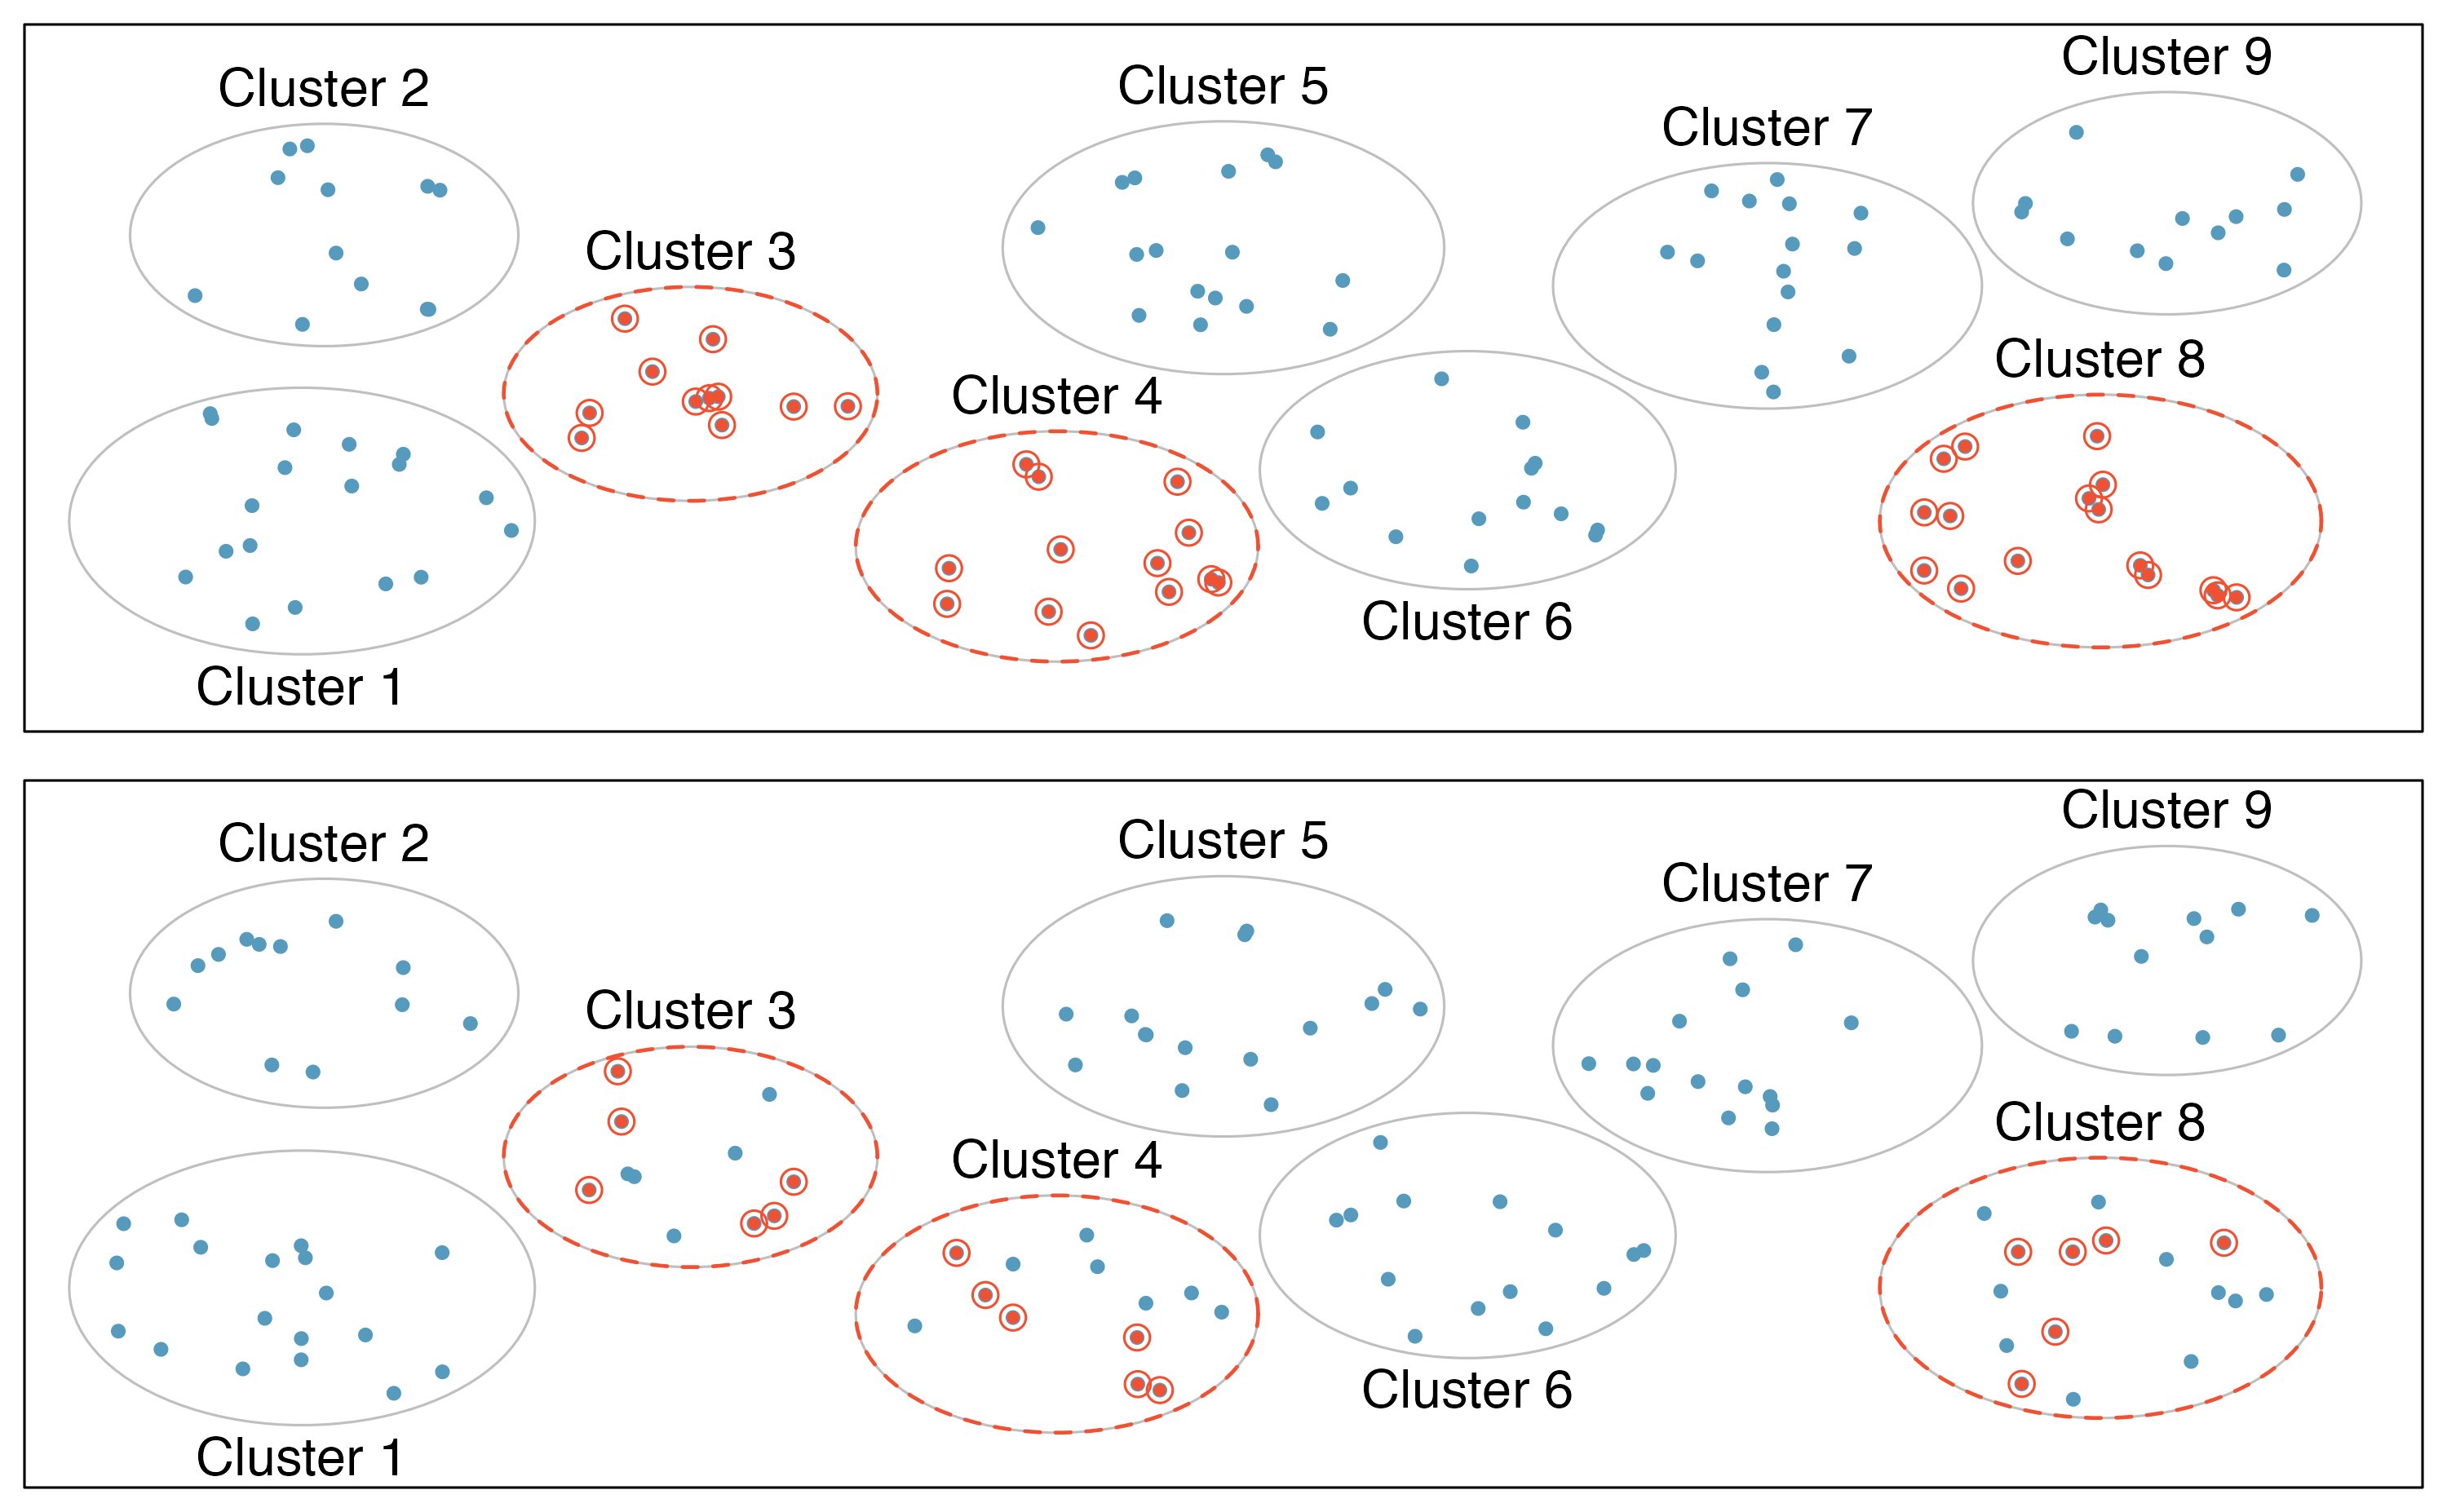
\includegraphics[width=0.8\textwidth,height=\textheight]{02-data-design_files/figure-pdf/fig-cluster-multistage-1.png}

}

\caption{\label{fig-cluster-multistage}Examples of cluster and
multistage sampling. In the top panel, cluster sampling was used: data
were binned into nine clusters, three of these clusters were sampled,
and all observations within these three clusters were included in the
sample. In the bottom panel, multistage sampling was used, which differs
from cluster sampling only in that we randomly select a subset of each
cluster to be included in the sample rather than measuring every case in
each sampled cluster.'}

\end{figure}%

Sometimes cluster or multistage sampling can be more economical than the
alternative sampling techniques. Also, unlike stratified sampling, these
approaches are most helpful when there is a lot of case-to-case
variability within a cluster but the clusters themselves do not look
very different from one another. For example, if neighborhoods
represented clusters, then cluster or multistage sampling work best when
the populations inside each neighborhood are very diverse. A downside of
these methods is that more advanced techniques are typically required to
analyze the data, though the methods in this book can be extended to
handle such data.

\begin{workedexample}
Suppose we are interested in estimating the malaria rate in a densely
tropical portion of rural Indonesia. We learn that there are 30 villages
in that part of the Indonesian jungle, each more or less like the next,
but the distances between the villages are substantial. We want to test
150 individuals for malaria. What sampling method should we use?

\begin{center}\rule{0.5\linewidth}{0.5pt}\end{center}

A simple random sample would likely draw individuals from all 30
villages, which could make data collection expensive. Stratified
sampling would be a challenge since it is unclear how we would build
strata of similar individuals. However, cluster sampling or multistage
sampling seem like very good ideas. With multistage sampling, we could
randomly select half of the villages, then randomly select 10 people
from each. This could reduce data collection costs substantially in
comparison to a simple random sample, and the cluster sample would still
yield reliable information, even if we would need to analyze the data
with more advanced methods than those introduced in this book.

\end{workedexample}

\section{Experiments}\label{sec-experiments}

Studies where the researchers assign treatments to cases are called
\textbf{experiments}\index{study!experiment}. When this assignment
includes randomization, e.g., using a coin flip to decide which
treatment a patient receives, it is called a \textbf{randomized
experiment}\index{study!randomized experiment}. Randomized experiments
are fundamentally important when trying to show a causal connection
between two variables.

\subsection{Principles of experimental
design}\label{sec-principles-experimental-design}

\begin{enumerate}
\def\labelenumi{\arabic{enumi}.}
\tightlist
\item
  \textbf{Controlling.} Researchers assign treatments to cases, and they
  do their best to \textbf{control}\index{control} any other differences
  in the groups\footnote{This is a different concept than a
    \emph{control group}, which we discuss in the second principle and
    in Section~\ref{sec-reducing-bias-human-experiments}.}. For example,
  when patients take a drug in pill form, some patients take the pill
  with only a sip of water while others may have it with an entire glass
  of water. To control for the effect of water consumption, a doctor may
  instruct every patient to drink a 12-ounce glass of water with the
  pill.
\end{enumerate}

\begin{enumerate}
\def\labelenumi{\arabic{enumi}.}
\setcounter{enumi}{1}
\tightlist
\item
  \textbf{Randomization.} Researchers randomize patients into treatment
  groups to account for variables that cannot be controlled. For
  example, some patients may be more susceptible to a disease than
  others due to their dietary habits. In this example dietary habit is a
  \textbf{confounding variable}\footnote{Also called a \textbf{lurking
    variable}, \textbf{confounding factor}, or a \textbf{confounder}.},
  which is defined as a variable that is associated with both the
  explanatory and response variables. Randomizing patients into the
  treatment or control group helps even out such differences.
\end{enumerate}

\begin{important}
\textbf{Confounding variable.}

A \textbf{confounding variable} is one that is associated with both the
explanatory and response variables. Because it is associated with both
variables, it prevents the study from concluding that the explanatory
variable caused the response variable. Consider a silly example with
total ice-cream sales as the explanatory variable and number of boating
accidents as the response variable (which may seem highly correlated).
Outside temperature is associated with both variables, and therefore we
cannot conclude that high ice-cream sales is a cause of more boating
accidents.

Confounding variables may or may not be measured as part of the study.
Regardless, drawing cause-and-effect conclusions is difficult in an
observational study because of the ever-present possibility of
confounding variables.

\end{important}

\index{confounding variable}

\begin{enumerate}
\def\labelenumi{\arabic{enumi}.}
\setcounter{enumi}{2}
\tightlist
\item
  \textbf{Replication.} The more cases researchers observe, the more
  accurately they can estimate the effect of the explanatory variable on
  the response. In a single study, we \textbf{replicate} by collecting a
  sufficiently large sample. What is considered sufficiently large
  varies from experiment to experiment, but at a minimum we want to have
  multiple subjects (experimental units) per treatment group. Another
  way of achieving replication is replicating an entire study to verify
  an earlier finding. The term \textbf{replication crisis} refers to the
  ongoing methodological crisis in which past findings from scientific
  studies in several disciplines have failed to be replicated.
  \textbf{Pseudoreplication} occurs when individual observations under
  different treatments are heavily dependent on each other. For example,
  suppose you have 50 subjects in an experiment where you're taking
  blood pressure measurements at 10 time points throughout the course of
  the study. By the end, you will have 50 \(\times\) 10 = 500
  measurements. Reporting that you have 500 observations would be
  considered pseudoreplication, as the blood pressure measurements of a
  given individual are not independent of each other. Pseudoreplication
  often happens when the wrong entity is replicated, and the reported
  sample sizes are exaggerated.
\end{enumerate}

\index{replication} \index{lurking variable}

\begin{enumerate}
\def\labelenumi{\arabic{enumi}.}
\setcounter{enumi}{3}
\tightlist
\item
  \textbf{Blocking.} Researchers sometimes know or suspect that
  variables, other than the treatment, influence the response. Under
  these circumstances, they may first group individuals based on this
  variable into \textbf{blocks} and then randomize cases within each
  block to the treatment groups. This strategy is often referred to as
  \textbf{blocking}. For instance, if we are looking at the effect of a
  drug on heart attacks, we might first split patients in the study into
  low-risk and high-risk blocks, then randomly assign half the patients
  from each block to the control group and the other half to the
  treatment group, as shown in Figure~\ref{fig-blocking}. This strategy
  ensures that each treatment group has the same number of low-risk
  patients and the same number of high-risk patients.
\end{enumerate}

\index{blocking}

\begin{figure}[H]

\centering{

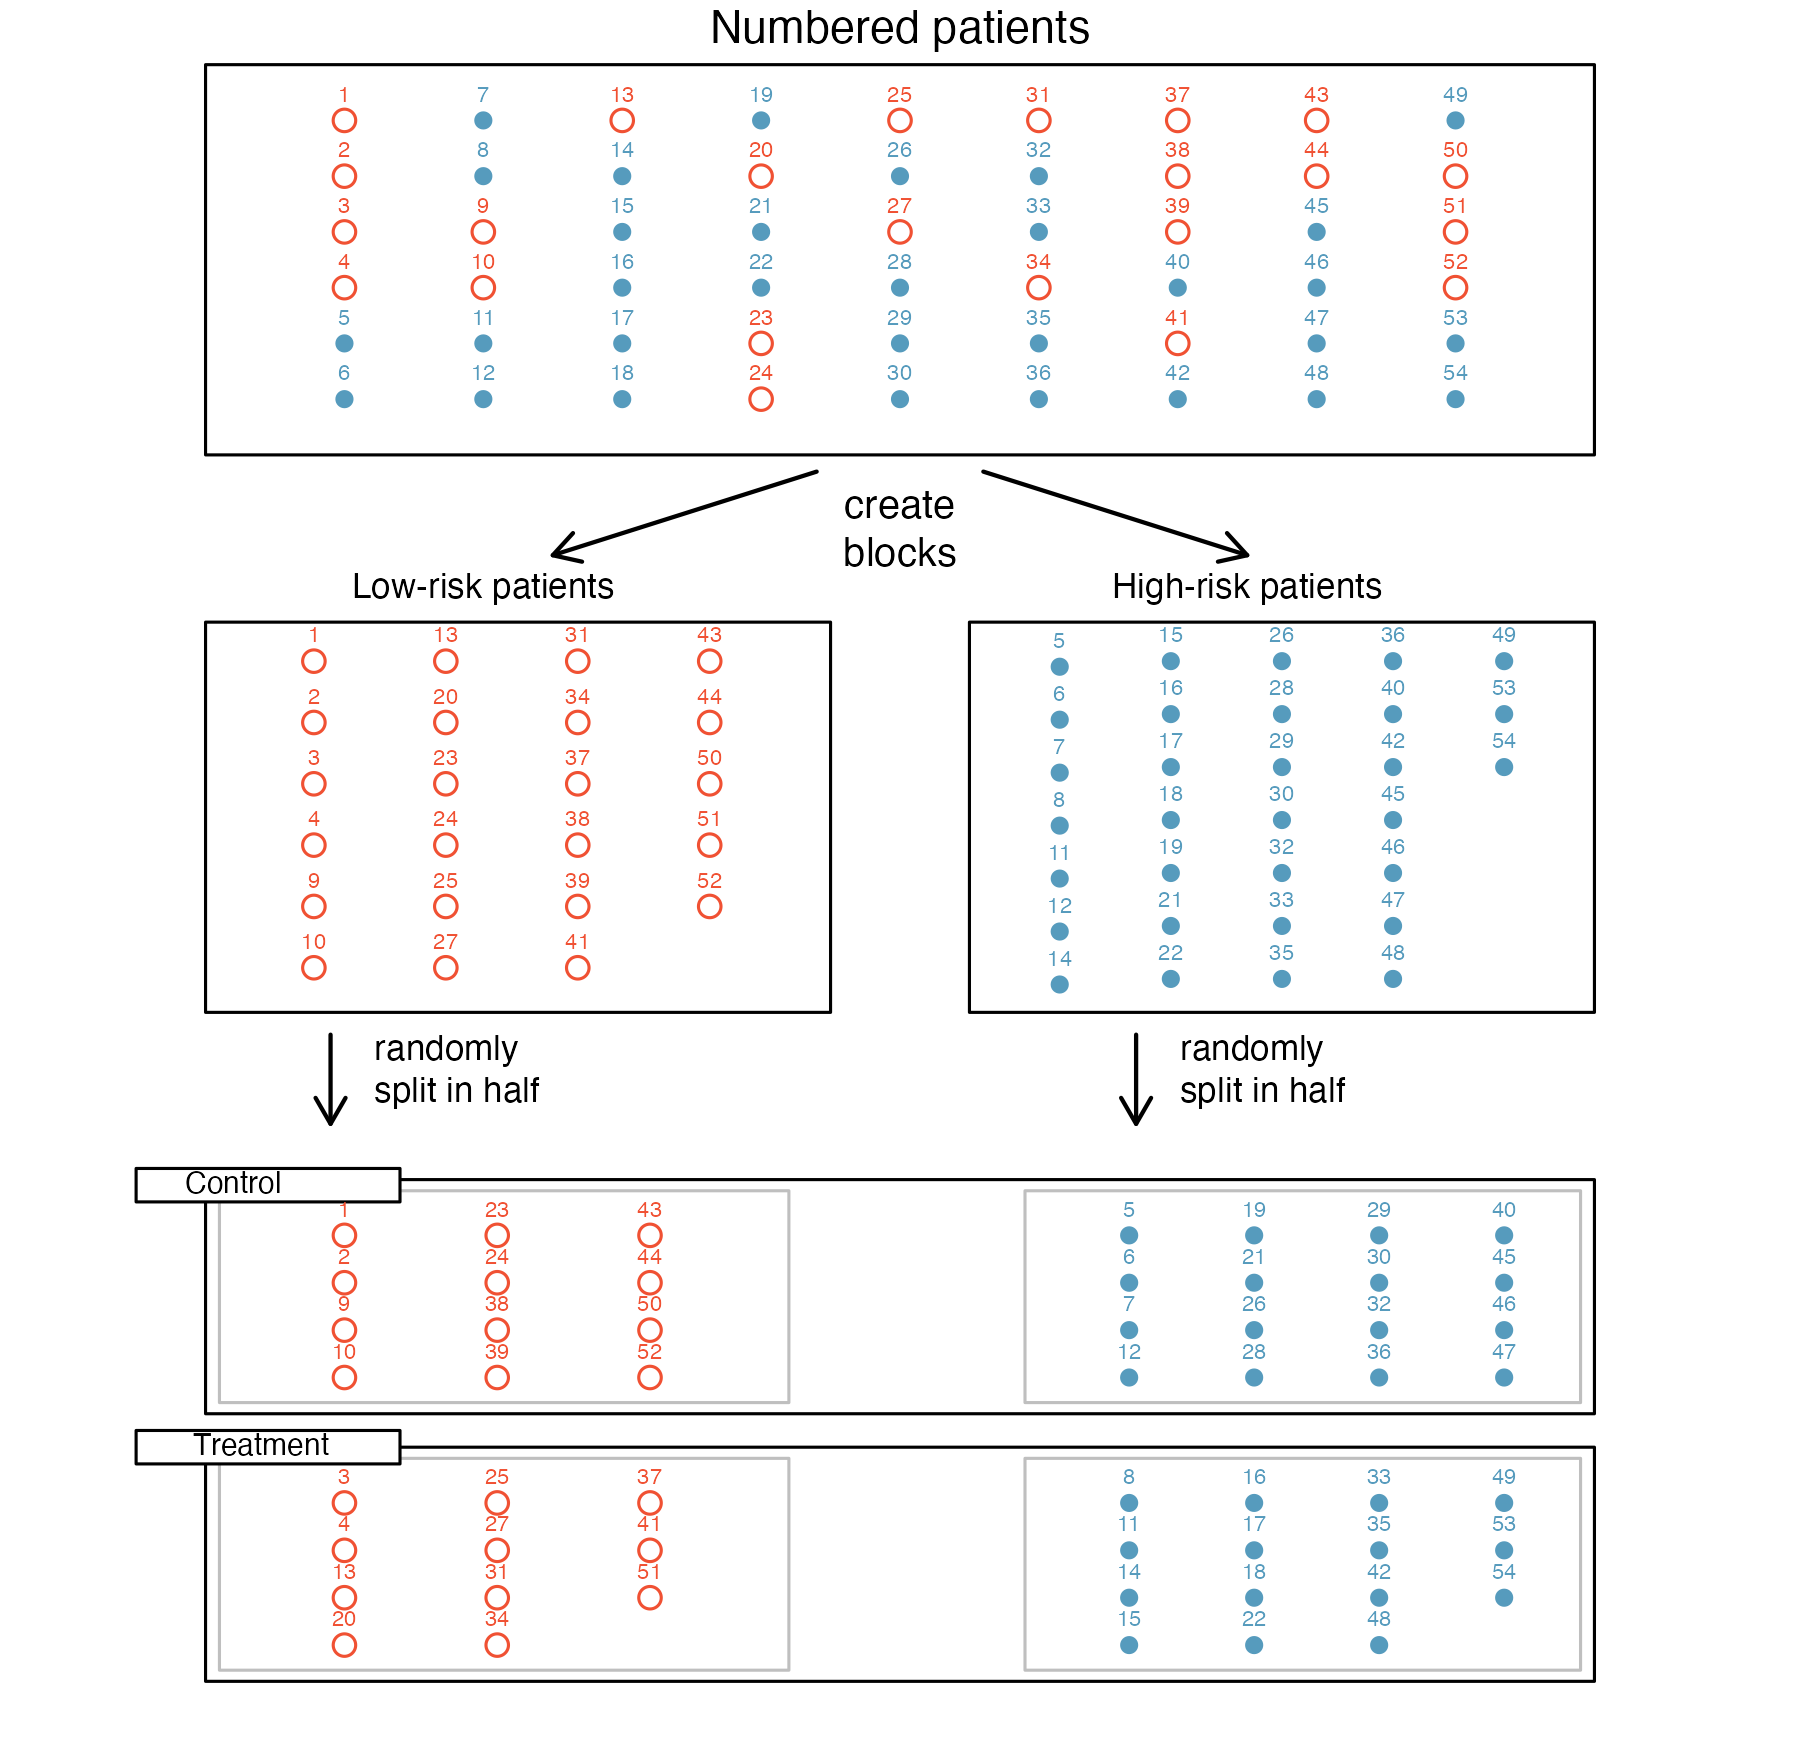
\includegraphics[width=0.87\textwidth,height=\textheight]{02-data-design_files/figure-pdf/fig-blocking-1.png}

}

\caption{\label{fig-blocking}Blocking for patient risk. Patients are
first divided into low-risk and high-risk blocks, then patients in each
block are evenly randomized into the treatment groups. This strategy
ensures equal representation of patients in each treatment group from
both risk categories.}

\end{figure}%

It is important to incorporate the first three experimental design
principles into any study, and this book describes applicable methods
for analyzing data from such experiments. Blocking is a slightly more
advanced technique, and statistical methods in this book may be extended
to analyze data collected using blocking.

\clearpage

\subsection{Reducing bias in human
experiments}\label{sec-reducing-bias-human-experiments}

Randomized experiments have long been considered to be the gold standard
for data collection, but they do not ensure an unbiased perspective into
the cause-and-effect relationship in all cases. Human studies are
perfect examples where bias can unintentionally arise. Here we
reconsider a study where a new drug was used to treat heart attack
patients. In particular, researchers wanted to know if the drug reduced
deaths in patients.

These researchers designed a randomized experiment because they wanted
to draw causal conclusions about the drug's effect. Study
volunteers\footnote{Human subjects are often called \textbf{patients},
  \textbf{volunteers}, or \textbf{study participants}.} were randomly
placed into two study groups. One group, the \textbf{treatment group},
received the drug. The other group, called the \textbf{control group},
did not receive any drug treatment.

Put yourself in the place of a person in the study. If you are in the
treatment group, you are given a fancy new drug that you anticipate will
help you. On the other hand, a person in the other group does not
receive the drug and sits idly, hoping her participation does not
increase her risk of death. These perspectives suggest there are
actually two effects in this study: the one of interest is the
effectiveness of the drug, and the second is an emotional effect of
(not) taking the drug, which is difficult to quantify.

Researchers aren't usually interested in the emotional effect, which
might bias the study. To circumvent this problem, researchers do not
want patients to know which group they are in. When researchers keep the
patients uninformed about their treatment, the study is said to be
\textbf{blind}. But there is one problem: if a patient does not receive
a treatment, they will know they're in the control group. A solution to
this problem is to give a fake treatment to patients in the control
group. This is called a \textbf{placebo}, and an effective placebo is
the key to making a study truly blind. A classic example of a placebo is
a sugar pill that is made to look like the actual treatment pill.
However, offering such a fake treatment may not be ethical in certain
experiments. For example, in medical experiments, typically the control
group must get the current standard of care. Oftentimes, a placebo
results in a slight but real improvement in patients. This effect has
been dubbed the \textbf{placebo effect}.

\index{blinding}

The patients are not the only ones who should be blinded: doctors and
researchers can unintentionally bias a study. When a doctor knows a
patient has been given the real treatment, they might inadvertently give
that patient more attention or care than a patient that they know is on
the placebo. To guard against this bias, which again has been found to
have a measurable effect in some instances, most modern studies employ a
\textbf{double-blind} setup where doctors or researchers who interact
with patients are, just like the patients, unaware of who is or is not
receiving the treatment.\footnote{There are always some researchers
  involved in the study who do know which patients are receiving which
  treatment. However, they do not interact with the study's patients and
  do not tell the blinded health care professionals who is receiving
  which treatment.}

\begin{guidedpractice}
Look back to the study in Section~\ref{sec-case-study-stents-strokes}
where researchers were testing whether stents were effective at reducing
strokes in at-risk patients. Is this an experiment? Was the study
blinded? Was it double-blinded?\footnote{The researchers assigned the
  patients into their treatment groups, so this study was an experiment.
  However, the patients could distinguish what treatment they received
  because a stent is a surgical procedure. There is no equivalent
  surgical placebo, so this study was not blind. The study could not be
  double-blind since it was not blind.}

\end{guidedpractice}

\begin{guidedpractice}
For the study in Section~\ref{sec-case-study-stents-strokes}, could the
researchers have employed a placebo? If so, what would that placebo have
looked like?\footnote{Ultimately, can we make patients think they got
  treated from a surgery? In fact, we can, and some experiments use a
  \textbf{sham surgery}. In a sham surgery, the patient does undergo
  surgery, but the patient does not receive the full treatment, though
  they will still get a placebo effect.}

\end{guidedpractice}

You may have many questions about the ethics of sham surgeries to create
a placebo. These questions may have even arisen in your mind when in the
general experiment context, where a possibly helpful treatment was
withheld from individuals in the control group; the main difference is
that a sham surgery tends to create additional risk, while withholding a
treatment only maintains a person's risk.

There are always multiple viewpoints of experiments and placebos, and
rarely is it obvious which is ethically ``correct''. For instance, is it
ethical to use a sham surgery when it creates a risk to the patient?
However, if we do not use sham surgeries, we may promote the use of a
costly treatment that has no real effect; if this happens, money and
other resources will be diverted away from other treatments that are
known to be helpful. Ultimately, this is a difficult situation where we
cannot perfectly protect both the patients who have volunteered for the
study and the patients who may benefit (or not) from the treatment in
the future.

\section{Observational studies}\label{sec-observational-studies}

Studies where no treatment has been explicitly applied (or explicitly
withheld) are called \textbf{observational studies}. For instance,
studies on the loan data and county data described in
Section~\ref{sec-data-basics} are would both be considered
observational, as they rely on \textbf{observational data}.

Making causal conclusions based on experiments is often reasonable,
since we can randomly assign the explanatory variable(s), i.e., the
treatments. However, making the same causal conclusions based on
observational data can be treacherous and is not recommended. Thus,
observational studies are generally only sufficient to show associations
or form hypotheses that can be later checked with experiments.

Suppose an observational study tracked sunscreen use and skin cancer,
and it was found that the more sunscreen someone used, the more likely
the person was to have skin cancer. Does this mean sunscreen
\emph{causes} skin cancer?

No! Some previous research tells us that using sunscreen actually
reduces skin cancer risk, so maybe there is another variable that can
explain this hypothetical association between sunscreen usage and skin
cancer, as shown in Figure~\ref{fig-sun-causes-cancer}. One important
piece of information that is absent is sun exposure. If someone is out
in the sun all day, they are more likely to use sunscreen \emph{and}
more likely to get skin cancer. Exposure to the sun is unaccounted for
in the simple observational investigation.

\begin{figure}[H]

\centering{

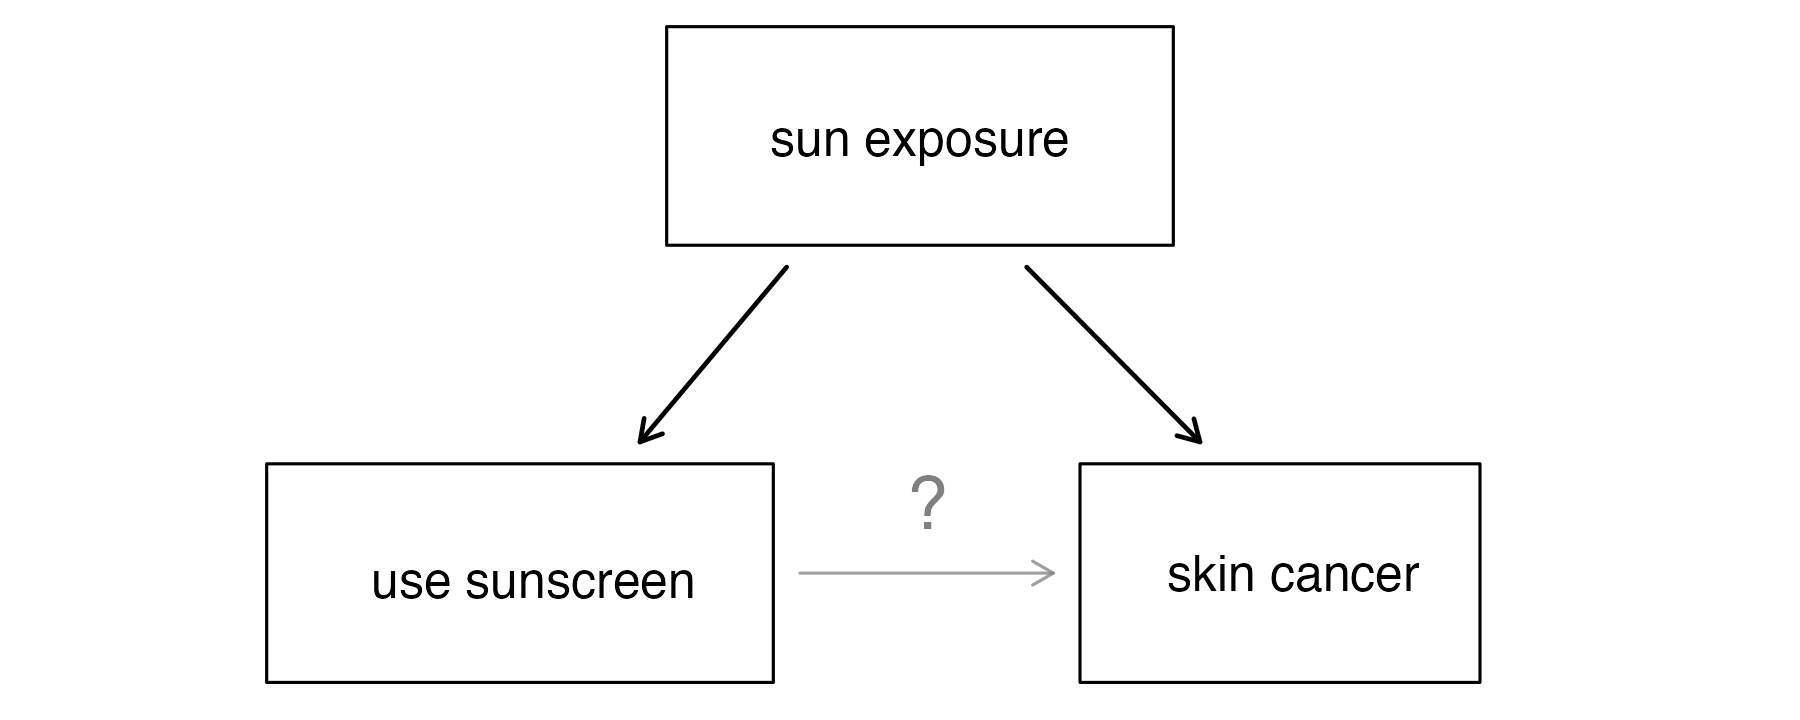
\includegraphics[width=0.6\textwidth,height=\textheight]{02-data-design_files/figure-pdf/fig-sun-causes-cancer-1.png}

}

\caption{\label{fig-sun-causes-cancer}Sun exposure may be the root cause
of both sunscreen use and skin cancer.}

\end{figure}%

In this example, sun exposure is a confounding variable. The presence of
confounding variables is what inhibits the ability for observational
studies to make causal claims. While one method to justify making causal
conclusions from observational studies is to exhaust the search for
confounding variables, there is no guarantee that all confounding
variables can be examined or measured.

\begin{guidedpractice}
Figure~\ref{fig-county-multi-unit-homeownership} shows a negative
association between the homeownership rate and the percentage of housing
units that are in multi-unit structures in a county. However, it is
unreasonable to conclude that there is a causal relationship between the
two variables. Suggest a variable that might explain the negative
relationship.\footnote{Answers will vary. Population density may be
  important. If a county is very dense, then this may require a larger
  percentage of residents to live in housing units that are in
  multi-unit structures. Additionally, the high density may contribute
  to increases in property value, making homeownership unfeasible for
  many residents.}

\end{guidedpractice}

Observational studies come in two forms: prospective and retrospective
studies. A \textbf{prospective study} identifies individuals and
collects information as events unfold. For instance, medical researchers
may identify and follow a group of patients over many years to assess
the possible influences of behavior on cancer risk. One example of such
a study is The Nurses' Health Study. Started in 1976 and expanded in
1989, the Nurses' Health Study has collected data on over 275,000 nurses
and is still enrolling participants. This prospective study recruits
registered nurses and then collects data from them using questionnaires.
\textbf{Retrospective studies} collect data after events have taken
place, e.g., researchers may review past events in medical records. Some
datasets may contain both prospectively- and retrospectively collected
variables, such as medical studies which gather information on
participants' lives before they enter the study and subsequently collect
data on participants throughout the study.

\index{study!prospective} \index{study!retrospective}

\clearpage

\section{Chapter review}\label{sec-chp2-review}

\subsection{Summary}\label{summary-1}

A proficient analyst will have a good sense of the types of data they
are working with and how to visualize the data in order to gain a
complete understanding of the variables. Equally important, however, is
the data source. In this chapter, we have discussed randomized
experiments and taking good, random, representative samples from a
population. When we discuss inferential methods (starting in
Chapter~\ref{sec-foundations-randomization}), the conclusions that can
be drawn will be dependent on how the data were collected.
Figure~\ref{fig-randsampValloc} summarizes how sampling and assignment
methods relate to the scope of inference.\footnote{Derived from similar
  figures in Chance and Rossman (2018) and Ramsey and Schafer (2012).}
Regularly revisiting Figure~\ref{fig-randsampValloc} will be important
when making conclusions from a given data analysis.

\begin{figure}[H]

\centering{

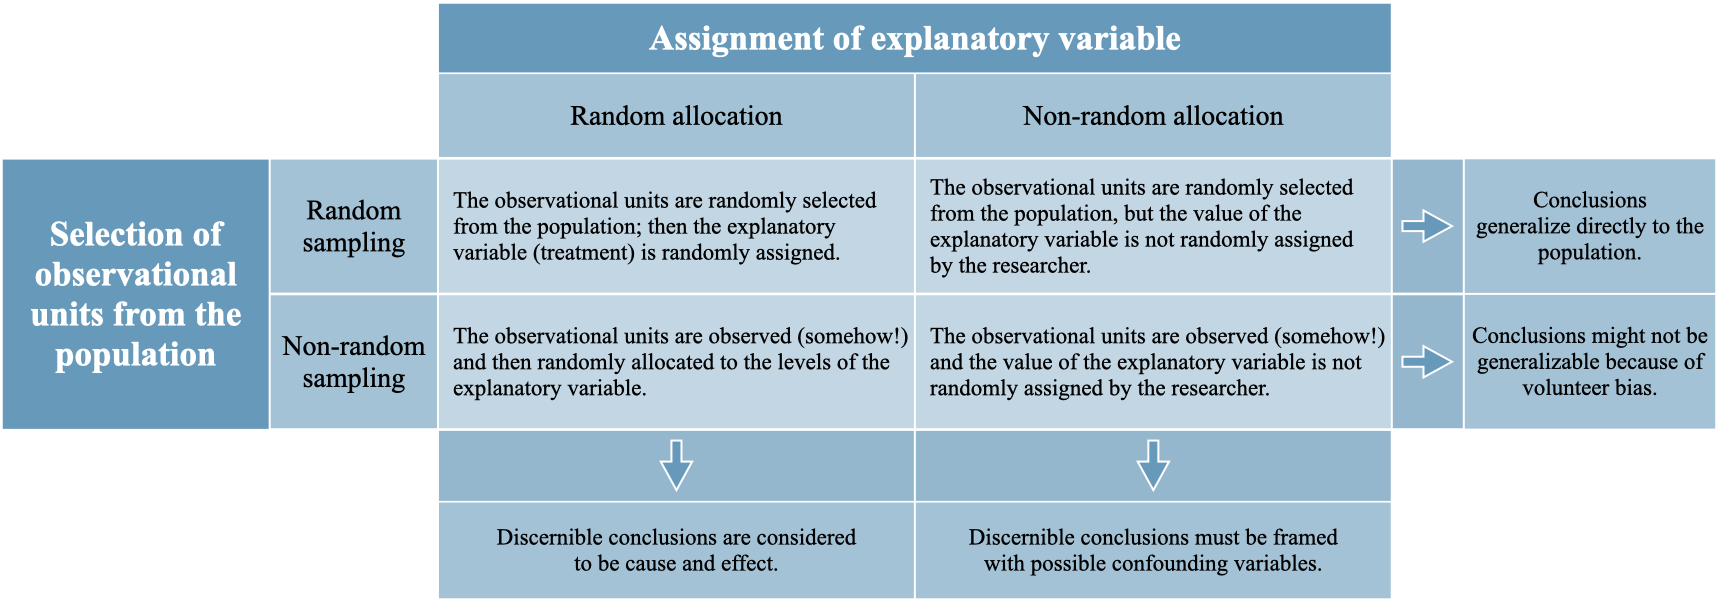
\includegraphics[width=0.96\textwidth,height=\textheight]{images/randsampValloc.png}

}

\caption{\label{fig-randsampValloc}Analysis conclusions should be made
carefully according to how the data were collected. Very few datasets
come from the top left box because usually ethics require that random
assignment of treatments can only be given to volunteers. Both
representative (ideally random) sampling and experiments (random
assignment of treatments) are important for how statistical conclusions
can be made on populations.}

\end{figure}%

\subsection{Terms}\label{terms-1}

The terms introduced in this chapter are presented in
Table~\ref{tbl-terms-chp-2}. If you're not sure what some of these terms
mean, we recommend you go back in the text and review their definitions.
You should be able to easily spot them as \textbf{bolded text}.

\begin{table}[H]

\caption{\label{tbl-terms-chp-2}Terms introduced in this chapter.}

\centering{

\centering
\begin{tabular}[t]{>{\raggedright\arraybackslash}p{12em}>{\raggedright\arraybackslash}p{12em}>{\raggedright\arraybackslash}p{12em}}
\toprule
\cellcolor{gray!10}{anecdotal evidence} & \cellcolor{gray!10}{experiment} & \cellcolor{gray!10}{replication}\\
bias & multistage sample & replication crisis\\
\cellcolor{gray!10}{blind} & \cellcolor{gray!10}{non-response bias} & \cellcolor{gray!10}{representative}\\
blocking & non-response rate & retrospective study\\
\cellcolor{gray!10}{census} & \cellcolor{gray!10}{observational study} & \cellcolor{gray!10}{sample}\\
cluster & placebo & sample bias\\
\cellcolor{gray!10}{cluster sampling} & \cellcolor{gray!10}{placebo effect} & \cellcolor{gray!10}{sample statistic}\\
confounding variable & population & simple random sample\\
\cellcolor{gray!10}{control} & \cellcolor{gray!10}{population parameter} & \cellcolor{gray!10}{simple random sampling}\\
control group & prospective study & strata\\
\cellcolor{gray!10}{convenience sample} & \cellcolor{gray!10}{pseudoreplication} & \cellcolor{gray!10}{stratified sampling}\\
double-blind & randomized experiment & treatment group\\
\bottomrule
\end{tabular}

}

\end{table}%

\clearpage

\section{Exercises}\label{sec-chp2-exercises}

Answers to odd-numbered exercises can be found in
Appendix~\ref{sec-exercise-solutions-02}.

\begin{exercises}

\begin{enumerate}
\def\labelenumi{\arabic{enumi}.}
\item
  \textbf{Parameters and statistics.} Identify which value represents
  the sample mean and which value represents the claimed population
  mean.

  \begin{enumerate}
  \def\labelenumii{\alph{enumii}.}
  \item
    American households spent an average of about \$52 in 2007 on
    Halloween merchandise such as costumes, decorations and candy. To
    see if this number had changed, researchers conducted a new survey
    in 2008 before industry numbers were reported. The survey included
    1,500 households and found that average Halloween spending was \$58
    per household.
  \item
    The average GPA of students in 2001 at a private university was
    3.37. A survey on a sample of 203 students from this university
    yielded an average GPA of 3.59 a decade later.
  \end{enumerate}
\end{enumerate}

\vfill

\begin{enumerate}
\def\labelenumi{\arabic{enumi}.}
\setcounter{enumi}{1}
\tightlist
\item
  \textbf{Sleeping in college.} A recent article in a college newspaper
  stated that college students get an average of 5.5 hrs of sleep each
  night. A student who was skeptical about this value decided to conduct
  a survey by randomly sampling 25 students. On average, the sampled
  students slept 6.25 hours per night. Identify which value represents
  the sample mean and which value represents the claimed population
  mean.
\end{enumerate}

\vfill

\begin{enumerate}
\def\labelenumi{\arabic{enumi}.}
\setcounter{enumi}{2}
\item
  \textbf{Air pollution and birth outcomes, scope of inference.}
  Researchers collected data to examine the relationship between air
  pollutants and preterm births in Southern California. During the study
  air pollution levels were measured by air quality monitoring stations.
  Length of gestation data were collected on 143,196 births between the
  years 1989 and 1993, and air pollution exposure during gestation was
  calculated for each birth. (Ritz et al. 2000)

  \begin{enumerate}
  \def\labelenumii{\alph{enumii}.}
  \item
    Identify the population of interest and the sample in this study.
  \item
    Comment on whether the results of the study can be generalized to
    the population, and if the findings of the study can be used to
    establish causal relationships.
  \end{enumerate}
\end{enumerate}

\vfill

\begin{enumerate}
\def\labelenumi{\arabic{enumi}.}
\setcounter{enumi}{3}
\item
  \textbf{Cheaters, scope of inference.} Researchers studying the
  relationship between honesty, age and self-control conducted an
  experiment on 160 children between the ages of 5 and 15. The
  researchers asked each child to toss a fair coin in private and to
  record the outcome (white or black) on a paper sheet, and said they
  would only reward children who report white. Half the students were
  explicitly told not to cheat and the others were not given any
  explicit instructions. Differences were observed in the cheating rates
  in the instruction and no instruction groups, as well as some
  differences across children's characteristics within each group.
  (Bucciol and Piovesan 2011)

  \begin{enumerate}
  \def\labelenumii{\alph{enumii}.}
  \item
    Identify the population of interest and the sample in this study.
  \item
    Comment on whether the results of the study can be generalized to
    the population, and if the findings of the study can be used to
    establish causal relationships.
  \end{enumerate}
\end{enumerate}

\vfill

\clearpage

\begin{enumerate}
\def\labelenumi{\arabic{enumi}.}
\setcounter{enumi}{4}
\item
  \textbf{Gamification and statistics, scope of inference.} Researchers
  investigating the effects of gamification (application of game-design
  elements and game principles in non-game contexts) on learning
  statistics randomly assigned 365 college students in a statistics
  course to one of four groups; one of these groups had no reading
  exercises and no gamification, one group had reading but no
  gamification, one group had gamification but no reading, and a final
  group had gamification and reading. Students in all groups also
  attended lectures. The study found that gamification had a positive
  impact on student learning compared to traditional teaching methods
  involving reading exercises. (Legaki et al. 2020)

  \begin{enumerate}
  \def\labelenumii{\alph{enumii}.}
  \item
    Identify the population of interest and the sample in this study.
  \item
    Comment on whether the results of the study can be generalized to
    the population, and if the findings of the study can be used to
    establish causal relationships.
  \end{enumerate}
\end{enumerate}

\vfill

\begin{enumerate}
\def\labelenumi{\arabic{enumi}.}
\setcounter{enumi}{5}
\item
  \textbf{Stealers, scope of inference.} In a study of the relationship
  between socio-economic class and unethical behavior, 129 University of
  California undergraduates at Berkeley were asked to identify
  themselves as having low or high social-class by comparing themselves
  to others with the most (least) money, most (least) education, and
  most (least) respected jobs. They were also presented with a jar of
  individually wrapped candies and informed that the candies were for
  children in a nearby laboratory, but that they could take some if they
  wanted. After completing some unrelated tasks, participants reported
  the number of candies they had taken. It was found that those who were
  identified as upper-class took more candy than others. (Piff et al.
  2012)

  \begin{enumerate}
  \def\labelenumii{\alph{enumii}.}
  \item
    Identify the population of interest and the sample in this study.
  \item
    Comment on whether the results of the study can be generalized to
    the population, and if the findings of the study can be used to
    establish causal relationships.
  \end{enumerate}
\end{enumerate}

\vfill

\begin{enumerate}
\def\labelenumi{\arabic{enumi}.}
\setcounter{enumi}{6}
\item
  \textbf{Relaxing after work.} The General Social Survey asked the
  question, \emph{``After an average work day, about how many hours do
  you have to relax or pursue activities that you enjoy?''} to a random
  sample of 1,155 Americans. The average relaxing time was found to be
  1.65 hours. Determine which of the following is an observation, a
  variable, a sample statistic, or a population parameter.\footnote{The
    data used in this exercise comes from the
    \href{https://www.openintro.org/go?id=textbook-gss-data&referrer=ims0_html}{General
    Social Survey, 2018}.}

  \begin{enumerate}
  \def\labelenumii{\alph{enumii}.}
  \item
    An American in the sample.
  \item
    Number of hours spent relaxing after an average work day.
  \item
    1.65.
  \item
    Average number of hours all Americans spend relaxing after an
    average work day.
  \end{enumerate}
\end{enumerate}

\vfill

\begin{enumerate}
\def\labelenumi{\arabic{enumi}.}
\setcounter{enumi}{7}
\item
  \textbf{Cats on YouTube.} Suppose you want to estimate the percentage
  of videos on YouTube that are cat videos. It is impossible for you to
  watch all videos on YouTube so you use a random video picker to select
  1000 videos for you. You find that 2\% of these videos are cat videos.
  Determine which of the following is an observation, a variable, a
  sample statistic, or a population parameter.

  \begin{enumerate}
  \def\labelenumii{\alph{enumii}.}
  \item
    Percentage of all videos on YouTube that are cat videos.
  \item
    2\%.
  \item
    A video in your sample.
  \item
    whether a video is a cat video.
  \end{enumerate}
\end{enumerate}

\vfill

\clearpage

\begin{enumerate}
\def\labelenumi{\arabic{enumi}.}
\setcounter{enumi}{8}
\item
  \textbf{Course satisfaction across sections.} A large college class
  has 160 students. All 160 students attend the lectures together, but
  the students are divided into 4 groups, each of 40 students, for lab
  sections administered by different teaching assistants. The professor
  wants to conduct a survey about how satisfied the students are with
  the course, and he believes that the lab section a student is in might
  affect the student's overall satisfaction with the course.

  \begin{enumerate}
  \def\labelenumii{\alph{enumii}.}
  \item
    What type of study is this?
  \item
    Suggest a sampling strategy for carrying out this study.
  \end{enumerate}
\end{enumerate}

\vfill

\begin{enumerate}
\def\labelenumi{\arabic{enumi}.}
\setcounter{enumi}{9}
\item
  \textbf{Housing proposal across dorms.} On a large college campus
  first-year students and sophomores live in dorms located on the
  eastern part of the campus and juniors and seniors live in dorms
  located on the western part of the campus. Suppose you want to collect
  student opinions on a new housing structure the college administration
  is proposing and you want to make sure your survey equally represents
  opinions from students from all years.

  \begin{enumerate}
  \def\labelenumii{\alph{enumii}.}
  \item
    What type of study is this?
  \item
    Suggest a sampling strategy for carrying out this study.
  \end{enumerate}
\end{enumerate}

\vfill

\begin{enumerate}
\def\labelenumi{\arabic{enumi}.}
\setcounter{enumi}{10}
\item
  \textbf{Internet use and life expectancy.} The following scatterplot
  was created as part of a study evaluating the relationship between
  estimated life expectancy at birth (as of 2014) and percentage of
  internet users (as of 2009) in 208 countries for which such data were
  available.\footnote{The
    \href{http://openintrostat.github.io/openintro/reference/cia_factbook.html}{\texttt{cia\_factbook}}
    data used in this exercise can be found in the
    \href{http://openintrostat.github.io/openintro}{\textbf{openintro}}
    R package.}

  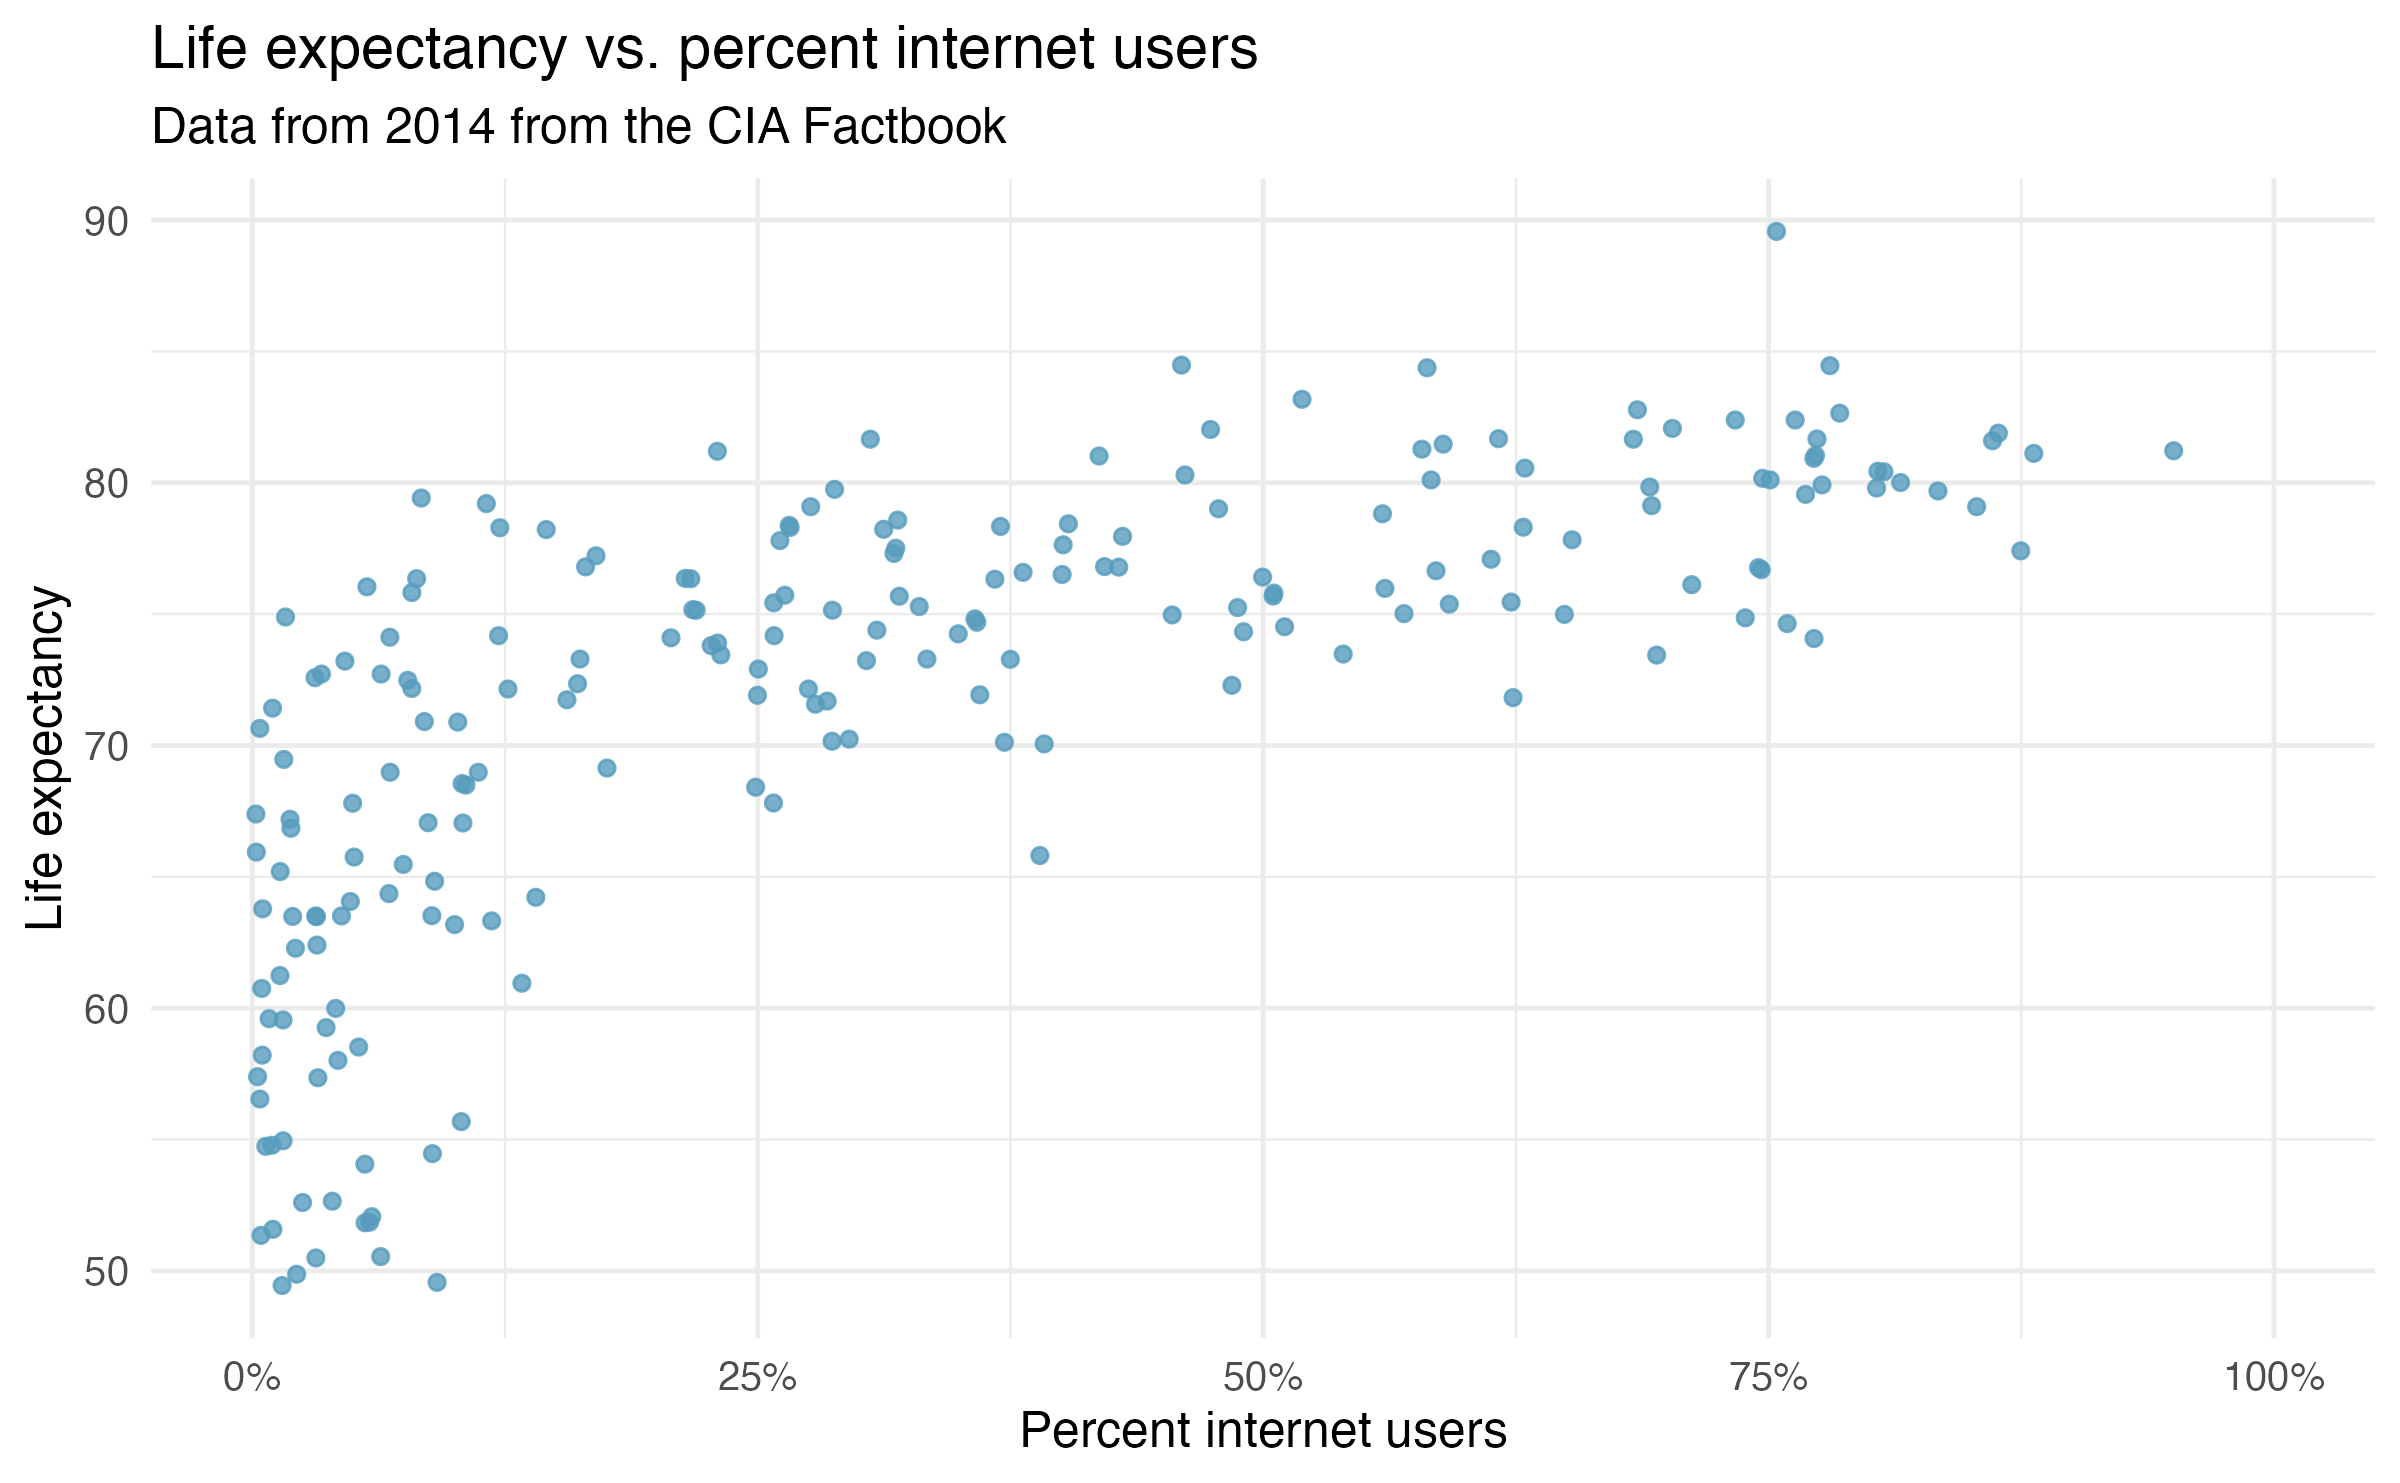
\includegraphics[width=0.8\textwidth,height=\textheight]{02-data-design_files/figure-pdf/unnamed-chunk-31-1.png}

  \begin{enumerate}
  \def\labelenumii{\alph{enumii}.}
  \item
    Describe the relationship between life expectancy and percentage of
    internet users.
  \item
    What type of study is this?
  \item
    State a possible confounding variable that might explain this
    relationship and describe its potential effect.
  \end{enumerate}
\end{enumerate}

\vfill

\clearpage

\begin{enumerate}
\def\labelenumi{\arabic{enumi}.}
\setcounter{enumi}{11}
\item
  \textbf{Stressed out.} A study that surveyed a random sample of
  otherwise healthy high school students found that they are more likely
  to get muscle cramps when they are stressed. The study also noted that
  students drink more coffee and sleep less when they are stressed.

  \begin{enumerate}
  \def\labelenumii{\alph{enumii}.}
  \item
    What type of study is this?
  \item
    Can this study be used to conclude a causal relationship between
    increased stress and muscle cramps?
  \item
    State possible confounding variables that might explain the observed
    relationship between increased stress and muscle cramps.
  \end{enumerate}
\item
  \textbf{Evaluate sampling methods.} A university wants to determine
  what fraction of its undergraduate student body support a new \$25
  annual fee to improve the student union. For each proposed method
  below, indicate whether the method is reasonable or not.

  \begin{enumerate}
  \def\labelenumii{\alph{enumii}.}
  \item
    Survey a simple random sample of 500 students.
  \item
    Stratify students by their field of study, then sample 10\% of
    students from each stratum.
  \item
    Cluster students by their ages (e.g., 18 years old in one cluster,
    19 years old in one cluster, etc.), then randomly sample three
    clusters and survey all students in those clusters.
  \end{enumerate}
\item
  \textbf{Random digit dialing.} The Gallup Poll uses a procedure called
  random digit dialing, which creates phone numbers based on a list of
  all area codes in America in conjunction with the associated number of
  residential households in each area code. Give a possible reason the
  Gallup Poll chooses to use random digit dialing instead of picking
  phone numbers from the phone book.
\item
  \textbf{Haters are gonna hate, study confirms.} A study published in
  the \emph{Journal of Personality and Social Psychology} asked a group
  of 200 randomly sampled participants recruited online using Amazon's
  Mechanical Turk to evaluate how they felt about various subjects, such
  as camping, health care, architecture, taxidermy, crossword puzzles,
  and Japan in order to measure their attitude towards mostly
  independent stimuli. Then, they presented the participants with
  information about a new product: a microwave oven. This microwave oven
  does not exist, but the participants didn't know this, and were given
  three positive and three negative fake reviews. People who reacted
  positively to the subjects on the dispositional attitude measurement
  also tended to react positively to the microwave oven, and those who
  reacted negatively tended to react negatively to it. Researchers
  concluded that \emph{``some people tend to like things, whereas others
  tend to dislike things, and a more thorough understanding of this
  tendency will lead to a more thorough understanding of the psychology
  of attitudes.''} (Hepler and Albarracı́n 2013)

  \begin{enumerate}
  \def\labelenumii{\alph{enumii}.}
  \item
    What are the cases?
  \item
    What is (are) the response variable(s) in this study?
  \item
    What is (are) the explanatory variable(s) in this study?
  \item
    Does the study employ random sampling? Explain your reasoning.
  \item
    Is this an observational study or an experiment? Explain your
    reasoning.
  \item
    Can we establish a causal link between the explanatory and response
    variables?
  \item
    Can the results of the study be generalized to the population at
    large?
  \end{enumerate}
\end{enumerate}

\clearpage

\begin{enumerate}
\def\labelenumi{\arabic{enumi}.}
\setcounter{enumi}{15}
\tightlist
\item
  \textbf{Family size.} Suppose we want to estimate household size,
  where a \emph{``household''} is defined as people living together in
  the same dwelling, and sharing living accommodations. If we select
  students at random at an elementary school and ask them what their
  family size is, will this be a good measure of household size? Or will
  our average be biased? If so, will it overestimate or underestimate
  the true value?
\end{enumerate}

\vfill

\begin{enumerate}
\def\labelenumi{\arabic{enumi}.}
\setcounter{enumi}{16}
\item
  \textbf{Sampling strategies.} A statistics student who is curious
  about the relationship between the amount of time students spend on
  social networking sites and their performance at school decides to
  conduct a survey. Various research strategies for collecting data are
  described below. In each, name the sampling method proposed and any
  bias you might expect.

  \begin{enumerate}
  \def\labelenumii{\alph{enumii}.}
  \item
    They randomly sample 40 students from the study's population, give
    them the survey, ask them to fill it out and bring it back the next
    day.
  \item
    They give out the survey only to their friends, making sure each one
    of them fills out the survey.
  \item
    They post a link to an online survey on Facebook and ask their
    friends to fill out the survey.
  \item
    They randomly sample 5 classes and asks a random sample of students
    from those classes to fill out the survey.
  \end{enumerate}
\end{enumerate}

\vfill

\begin{enumerate}
\def\labelenumi{\arabic{enumi}.}
\setcounter{enumi}{17}
\item
  \textbf{Reading the paper.} Below are excerpts from two articles
  published in the \emph{NY Times}:

  \begin{enumerate}
  \def\labelenumii{\alph{enumii}.}
  \tightlist
  \item
    An excerpt from an article titled \emph{Risks: Smokers Found More
    Prone to Dementia} is below. Based on this study, can we conclude
    that smoking causes dementia later in life? Explain your reasoning.
    (Rabin 2010)
  \end{enumerate}

  \begin{quote}
  ``Researchers analyzed data from 23,123 health plan members who
  participated in a voluntary exam and health behavior survey from 1978
  to 1985, when they were 50-60 years old. 23 years later, about 25\% of
  the group had dementia, including 1,136 with Alzheimer's disease and
  416 with vascular dementia. After adjusting for other factors, the
  researchers concluded that pack-a-day smokers were 37\% more likely
  than nonsmokers to develop dementia, and the risks went up with
  increased smoking; 44\% for one to two packs a day; and twice the risk
  for more than two packs.''
  \end{quote}

  \begin{enumerate}
  \def\labelenumii{\alph{enumii}.}
  \setcounter{enumii}{1}
  \tightlist
  \item
    An excerpt from an article titled \emph{The School Bully Is Sleepy}
    is below. A friend of yours who read the article says, \emph{``The
    study shows that sleep disorders lead to bullying in school
    children.''} Is this statement justified? If not, how best can you
    describe the conclusion that can be drawn from this study?
    (Parker-Pope 2011)
  \end{enumerate}

  \begin{quote}
  ``The University of Michigan study, collected survey data from parents
  on each child's sleep habits and asked both parents and teachers to
  assess behavioral concerns. About a third of the students studied were
  identified by parents or teachers as having problems with disruptive
  behavior or bullying. The researchers found that children who had
  behavioral issues and those who were identified as bullies were twice
  as likely to have shown symptoms of sleep disorders.''
  \end{quote}
\end{enumerate}

\vfill

\clearpage

\begin{enumerate}
\def\labelenumi{\arabic{enumi}.}
\setcounter{enumi}{18}
\item
  \textbf{Light and exam performance.} A study is designed to test the
  effect of light level on exam performance of students. The researcher
  believes that light levels might have different effects on people who
  wear glasses and people who don't, so they want to make sure both
  groups of people are equally represented in each treatment. The
  treatments are fluorescent overhead lighting, yellow overhead
  lighting, no overhead lighting (only desk lamps).

  \begin{enumerate}
  \def\labelenumii{\alph{enumii}.}
  \item
    What is the response variable?
  \item
    What is the explanatory variable? What are its levels?
  \item
    What is the blocking variable? What are its levels?
  \end{enumerate}
\item
  \textbf{Vitamin supplements.} To assess the effectiveness of taking
  large doses of vitamin C in reducing the duration of the common cold,
  researchers recruited 400 healthy volunteers from staff and students
  at a university. A quarter of the patients were assigned a placebo,
  and the rest were evenly divided between 1g Vitamin C, 3g Vitamin C,
  or 3g Vitamin C plus additives to be taken at onset of a cold for the
  following two days. All tablets had identical appearance and
  packaging. The nurses who handed the prescribed pills to the patients
  knew which patient received which treatment, but the researchers
  assessing the patients when they were sick did not. No statistically
  discernible differences were observed in any measure of cold duration
  or severity between the four groups, and the placebo group had the
  shortest duration of symptoms. (Audera et al. 2001)

  \begin{enumerate}
  \def\labelenumii{\alph{enumii}.}
  \item
    Was this an experiment or an observational study? Why?
  \item
    What are the explanatory and response variables in this study?
  \item
    Were the patients blinded to their treatment?
  \item
    Was this study double-blind?
  \item
    Participants are ultimately able to choose whether to use the pills
    prescribed to them. We might expect that not all of them will adhere
    and take their pills. Does this introduce a confounding variable to
    the study? Explain your reasoning.
  \end{enumerate}
\item
  \textbf{Light, noise, and exam performance.} A study is designed to
  test the effect of light level and noise level on exam performance of
  students. The researcher believes that light and noise levels might
  have different effects on people who wear glasses and people who
  don't, so they want to make sure both groups of people are equally
  represented in each treatment. The light treatments considered are
  fluorescent overhead lighting, yellow overhead lighting, no overhead
  lighting (only desk lamps). The noise treatments considered are no
  noise, construction noise, and human chatter noise.

  \begin{enumerate}
  \def\labelenumii{\alph{enumii}.}
  \item
    What type of study is this?
  \item
    How many factors are considered in this study? Identify them, and
    describe their levels.
  \item
    What is the role of the wearing glasses variable in this study?
  \end{enumerate}
\item
  \textbf{Music and learning.} You would like to conduct an experiment
  in class to see if students learn better if they study without any
  music, with music that has no lyrics (instrumental), or with music
  that has lyrics. Briefly outline a design for this study.
\item
  \textbf{Soda preference.} You would like to conduct an experiment in
  class to see if your classmates prefer the taste of regular Coke or
  Diet Coke. Briefly outline a design for this study.
\end{enumerate}

\clearpage

\begin{enumerate}
\def\labelenumi{\arabic{enumi}.}
\setcounter{enumi}{23}
\item
  \textbf{Exercise and mental health.} A researcher is interested in the
  effects of exercise on mental health and they propose the following
  study: use stratified random sampling to ensure representative
  proportions of 18-30, 31-40 and 41- 55 year-olds from the population.
  Next, randomly assign half the subjects from each age group to
  exercise twice a week, and instruct the rest not to exercise. Conduct
  a mental health exam at the beginning and at the end of the study, and
  compare the results.

  \begin{enumerate}
  \def\labelenumii{\alph{enumii}.}
  \item
    What type of study is this?
  \item
    What are the treatment and control groups in this study?
  \item
    Does this study make use of blocking? If so, what is the blocking
    variable?
  \item
    Does this study make use of blinding?
  \item
    Comment on whether the results of the study can be used to establish
    a causal relationship between exercise and mental health, and
    indicate whether the conclusions can be generalized to the
    population at large.
  \item
    Suppose you are given the task of determining if this proposed study
    should get funding. Would you have any reservations about the study
    proposal?
  \end{enumerate}
\end{enumerate}

\vspace{-1mm}

\begin{enumerate}
\def\labelenumi{\arabic{enumi}.}
\setcounter{enumi}{24}
\item
  \textbf{Chia seeds and weight loss.} Chia Pets -- those terra-cotta
  figurines that sprout fuzzy green hair -- made the chia plant a
  household name. But chia has since gained a reputation as a diet
  supplement. In one 2009 study, 38 men and 38 women were recruited and
  and divided each randomly into two groups: treatment or control. One
  group was given 25 grams of chia seeds twice a day, and the other was
  given a placebo. The subjects volunteered to be a part of the study.
  After 12 weeks, the scientists found no statistically discernible
  difference between the groups in appetite or weight loss. (Nieman et
  al. 2009)

  \begin{enumerate}
  \def\labelenumii{\alph{enumii}.}
  \item
    What type of study is this?
  \item
    What are the experimental and control treatments in this study?
  \item
    Has blocking been used in this study? If so, what is the blocking
    variable?
  \item
    Has blinding been used in this study?
  \item
    Comment on whether we can make a causal statement, and indicate
    whether we can generalize the conclusion to the population at large.
  \end{enumerate}
\end{enumerate}

\vspace{-1mm}

\begin{enumerate}
\def\labelenumi{\arabic{enumi}.}
\setcounter{enumi}{25}
\item
  \textbf{City council survey.} A city council has requested a household
  survey be conducted in a suburban area of their city. The area is
  broken into many distinct and unique neighborhoods, some including
  large homes, some with only apartments, and others a diverse mixture
  of housing structures. For each part below, identify the sampling
  methods described, and describe the statistical pros and cons of the
  method in the city's context.

  \begin{enumerate}
  \def\labelenumii{\alph{enumii}.}
  \item
    Randomly sample 200 households from the city.
  \item
    Divide the city into 20 neighborhoods, and then sample 10 households
    from each neighborhood.
  \item
    Divide the city into 20 neighborhoods, randomly sample 3
    neighborhoods, and then sample all households from those 3
    neighborhoods.
  \item
    Divide the city into 20 neighborhoods, randomly sample 8
    neighborhoods, and then randomly sample 50 households from those
    neighborhoods.
  \item
    Sample the 200 households closest to the city council offices.
  \end{enumerate}
\end{enumerate}

\clearpage

\begin{enumerate}
\def\labelenumi{\arabic{enumi}.}
\setcounter{enumi}{26}
\item
  \textbf{Flawed reasoning.} Identify the flaw(s) in reasoning in the
  following scenarios. Explain what the individuals in the study should
  have done differently if they wanted to make such strong conclusions.

  \begin{enumerate}
  \def\labelenumii{\alph{enumii}.}
  \item
    Students at an elementary school are given a questionnaire that they
    are asked to return after their parents have completed it. One of
    the questions asked is, \emph{``Do you find that your work schedule
    makes it difficult for you to spend time with your kids after
    school?''} Of the parents who replied, 85\% said \emph{``no''}.
    Based on these results, the school officials conclude that a great
    majority of the parents have no difficulty spending time with their
    kids after school.
  \item
    A survey is conducted on a simple random sample of 1,000 women who
    recently gave birth, asking them about whether they smoked during
    pregnancy. A follow-up survey asking if the children have
    respiratory problems is conducted 3 years later. However, only 567
    of these women are reached at the same address. The researcher
    reports that these 567 women are representative of all mothers.
  \item
    An orthopedist administers a questionnaire to 30 of his patients who
    do not have any joint problems and finds that 20 of them regularly
    go running. He concludes that running decreases the risk of joint
    problems.
  \end{enumerate}
\end{enumerate}

\vfill

\begin{enumerate}
\def\labelenumi{\arabic{enumi}.}
\setcounter{enumi}{27}
\item
  \textbf{Income and education in US counties.} The scatterplot below
  shows the relationship between per capita income (in thousands of
  dollars) and percent of population with a bachelor's degree in 3,142
  counties in the US in 2019.\footnote{The
    \href{http://openintrostat.github.io/openintro/reference/county_complete.html}{\texttt{county\_complete}}
    data used in this exercise can be found in the
    \href{http://openintrostat.github.io/openintro}{\textbf{openintro}}
    R package.}

  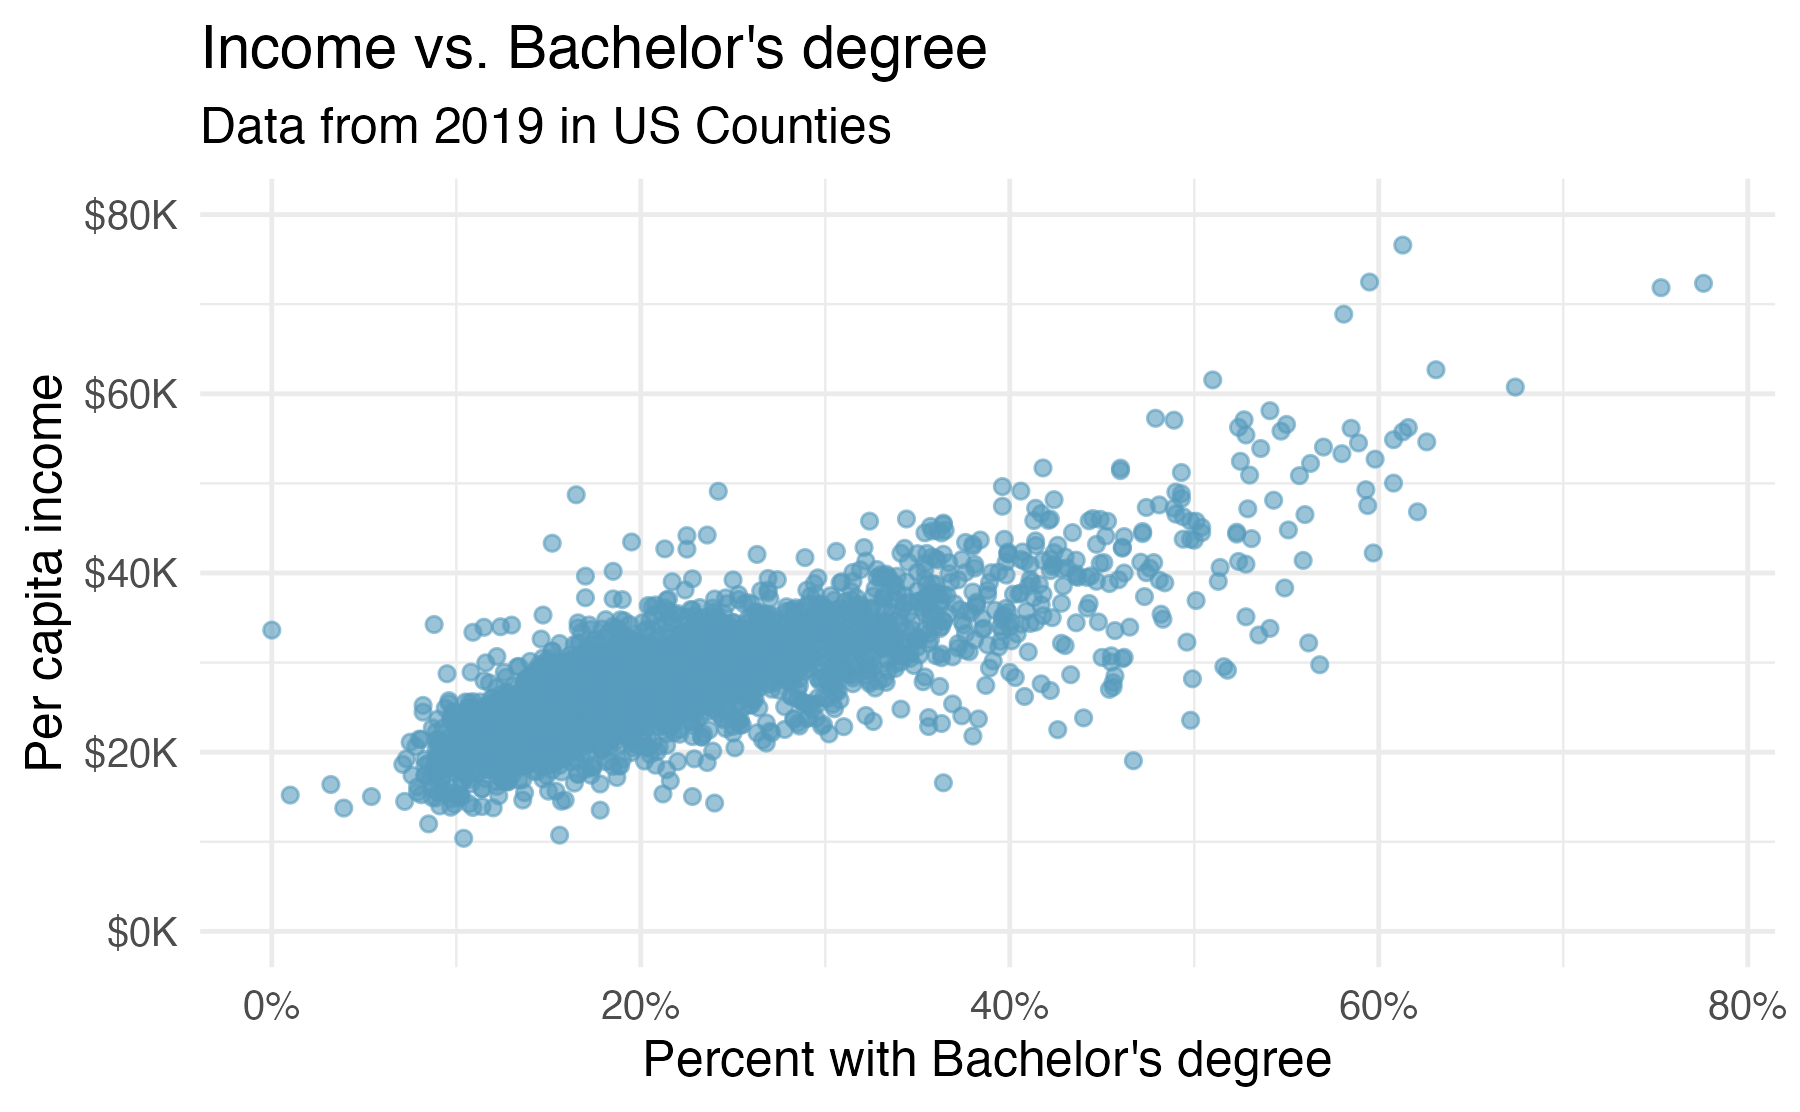
\includegraphics[width=0.8\textwidth,height=\textheight]{02-data-design_files/figure-pdf/unnamed-chunk-32-1.png}

  \begin{enumerate}
  \def\labelenumii{\alph{enumii}.}
  \item
    What are the explanatory and response variables?
  \item
    Describe the relationship between the two variables. Make sure to
    discuss unusual observations, if any.
  \item
    Can we conclude that having a bachelor's degree increases one's
    income?
  \end{enumerate}
\end{enumerate}

\vfill

\clearpage

\begin{enumerate}
\def\labelenumi{\arabic{enumi}.}
\setcounter{enumi}{28}
\item
  \textbf{Eat well, feel better.} In a public health study on the
  effects of consumption of fruits and vegetables on psychological
  well-being in young adults, participants were randomly assigned to
  three groups: (1) diet-as-usual, (2) an ecological momentary
  intervention involving text message reminders to increase their fruits
  and vegetable consumption plus a voucher to purchase them, or (3) a
  fruit and vegetable intervention in which participants were given two
  additional daily servings of fresh fruits and vegetables to consume on
  top of their normal diet. Participants were asked to take a nightly
  survey on their smartphones. Participants were student volunteers at
  the University of Otago, New Zealand. At the end of the 14-day study,
  only participants in the third group showed improvements to their
  psychological well-being across the 14-days relative to the other
  groups. (Conner et al. 2017)

  \begin{enumerate}
  \def\labelenumii{\alph{enumii}.}
  \item
    What type of study is this?
  \item
    Identify the explanatory and response variables.
  \item
    Comment on whether the results of the study can be generalized to
    the population.
  \item
    Comment on whether the results of the study can be used to establish
    causal relationships.
  \item
    A newspaper article reporting on the study states, ``The results of
    this study provide proof that giving young adults fresh fruits and
    vegetables to eat can have psychological benefits, even over a brief
    period of time.'' How would you suggest revising this statement so
    that it can be supported by the study?
  \end{enumerate}
\item
  \textbf{Screens, teens, and psychological well-being.} In a study of
  three nationally representative large-scale datasets from Ireland, the
  United States, and the United Kingdom (n = 17,247), teenagers between
  the ages of 12 to 15 were asked to keep a diary of their screen time
  and answer questions about how they felt or acted. The answers to
  these questions were then used to compute a psychological well-being
  score. Additional data were collected and included in the analysis,
  such as each child's sex and age, and on the mother's education,
  ethnicity, psychological distress, and employment. The study concluded
  that there is little clear-cut evidence that screen time decreases
  adolescent well-being. (Orben and Baukney-Przybylski 2018)

  \begin{enumerate}
  \def\labelenumii{\alph{enumii}.}
  \item
    What type of study is this?
  \item
    Identify the explanatory variables.
  \item
    Identify the response variable.
  \item
    Comment on whether the results of the study can be generalized to
    the population, and why.
  \item
    Comment on whether the results of the study can be used to establish
    causal relationships.
  \end{enumerate}
\end{enumerate}

\end{exercises}

\chapter{Applications: Data}\label{sec-data-applications}

\section{Case study: Olympic 1500m}\label{sec-case-study-paralympics}

While many of you may be glued to the Olympic Games every four years (or
every two years if you fancy both summer and winter sports), the
Paralympic Games are less popular than the Olympic Games, even if they
hold the same competitive thrills.

The Paralympic Games began as a way to support soldiers who had been
wounded in World War II as a way to help them rehabilitate. The first
Paralympic Games were held in Rome, Italy in 1960. Since 1988 (Seoul,
South Korea), the Paralympic Games have been held a few weeks later than
the Olympic Games in the same city, in both the summer and winter.

In this case study we introduce a dataset comparing Olympic and
Paralympic gold medal finishers in the 1500m running competition (the
Olympic ``mile'', if a bit shorter than a full mile). The goal of the
case study is to walk you through what a data scientist does when they
first get a hold of a dataset. We also provide some ``foreshadowing'' of
concepts and techniques we'll introduce in the next few chapters on
exploratory data analysis. Last, we introduce
\href{https://en.wikipedia.org/wiki/Simpson\%27s_paradox}{Simpson's
paradox} and discuss the importance of understanding the impact of
multiple variables in an analysis.

\begin{data}
The
\href{http://openintrostat.github.io/openintro/reference/paralympic_1500.html}{\texttt{paralympic\_1500}}
data can be found in the
\href{http://openintrostat.github.io/openintro/}{openintro} R package.

\end{data}

Table~\ref{tbl-paralympic-df-tail} shows the last five rows from the
dataset, which are the five most recent 1500m races. Notice that there
are racers from both the Men's and Women's divisions as well as those of
varying visual impairment (T11, T12, T13, and Olympic). The T11 athletes
have almost complete visual impairment, run with a black-out blindfold,
and are allowed to run with a guide-runner. T12 and T13 athletes have
some visual impairment, and the visual acuity of Olympic runners is not
determined.

\begin{table}

\caption{\label{tbl-paralympic-df-tail}Last five rows of the
\texttt{paralympic\_1500} dataset.}

\centering{

\centering
\begin{tabular}[t]{rr>{\raggedright\arraybackslash}p{3em}>{\raggedright\arraybackslash}p{4em}ll>{\raggedright\arraybackslash}p{5em}>{\raggedright\arraybackslash}p{5em}l>{\raggedleft\arraybackslash}p{4em}}
\toprule
 & year & city & country\_of\_games & division & type & name & country\_of\_athlete & time & time\_min\\
\midrule
\cellcolor{gray!10}{78} & \cellcolor{gray!10}{2020} & \cellcolor{gray!10}{Tokyo} & \cellcolor{gray!10}{Japan} & \cellcolor{gray!10}{Men} & \cellcolor{gray!10}{T11} & \cellcolor{gray!10}{Yeltsin Jacques} & \cellcolor{gray!10}{Brazil} & \cellcolor{gray!10}{3:57.6} & \cellcolor{gray!10}{3.96}\\
79 & 2020 & Tokyo & Japan & Men & T13 & Anton Kuliatin & Russian Paralympic Committee & 3:54.04 & 3.90\\
\cellcolor{gray!10}{80} & \cellcolor{gray!10}{2020} & \cellcolor{gray!10}{Tokyo} & \cellcolor{gray!10}{Japan} & \cellcolor{gray!10}{Women} & \cellcolor{gray!10}{Olympic} & \cellcolor{gray!10}{Faith Chepngetich Kipyegon} & \cellcolor{gray!10}{Kenya} & \cellcolor{gray!10}{3:53.11} & \cellcolor{gray!10}{3.88}\\
81 & 2020 & Tokyo & Japan & Women & T11 & Monica Olivia Rodriguez Saavedra & Mexico & 4:37.4 & 4.62\\
\cellcolor{gray!10}{82} & \cellcolor{gray!10}{2020} & \cellcolor{gray!10}{Tokyo} & \cellcolor{gray!10}{Japan} & \cellcolor{gray!10}{Women} & \cellcolor{gray!10}{T13} & \cellcolor{gray!10}{Tigist Gezahagn Menigstu} & \cellcolor{gray!10}{Ethiopia} & \cellcolor{gray!10}{4:23.24} & \cellcolor{gray!10}{4.39}\\
\bottomrule
\end{tabular}

}

\end{table}%

When you encounter a new dataset, taking a peek at the last few rows as
we did in Table~\ref{tbl-paralympic-df-tail} should be instinctual. It
can be helpful to look at the first few rows of the data as well to get
a sense of other aspects of the data which may not be apparent in the
last few rows. Table~\ref{tbl-paralympic-df-head} shows the top five
rows of the \texttt{paralympic\_1500} dataset, which reveals that for at
least the first five Olympiads, there were no runners in the Women's
division or in the Paralympics.

\begin{table}

\caption{\label{tbl-paralympic-df-head}First five rows of the
\texttt{paralympic\_1500} dataset.}

\centering{

\centering
\begin{tabular}[t]{rr>{\raggedright\arraybackslash}p{3em}>{\raggedright\arraybackslash}p{4em}ll>{\raggedright\arraybackslash}p{5em}>{\raggedright\arraybackslash}p{5em}l>{\raggedleft\arraybackslash}p{4em}}
\toprule
 & year & city & country\_of\_games & division & type & name & country\_of\_athlete & time & time\_min\\
\midrule
\cellcolor{gray!10}{1} & \cellcolor{gray!10}{1896} & \cellcolor{gray!10}{Athens} & \cellcolor{gray!10}{Greece} & \cellcolor{gray!10}{Men} & \cellcolor{gray!10}{Olympic} & \cellcolor{gray!10}{Edwin Flack} & \cellcolor{gray!10}{Australia} & \cellcolor{gray!10}{4:33.2} & \cellcolor{gray!10}{4.55}\\
2 & 1900 & Paris & France & Men & Olympic & Charles Bennett & Great Britain & 4:6.2 & 4.10\\
\cellcolor{gray!10}{3} & \cellcolor{gray!10}{1904} & \cellcolor{gray!10}{St Louis} & \cellcolor{gray!10}{USA} & \cellcolor{gray!10}{Men} & \cellcolor{gray!10}{Olympic} & \cellcolor{gray!10}{Jim Lightbody} & \cellcolor{gray!10}{USA} & \cellcolor{gray!10}{4:5.4} & \cellcolor{gray!10}{4.09}\\
4 & 1908 & London & United Kingdom & Men & Olympic & Mel Sheppard & USA & 4:3.4 & 4.06\\
\cellcolor{gray!10}{5} & \cellcolor{gray!10}{1912} & \cellcolor{gray!10}{Stockholm} & \cellcolor{gray!10}{Sweden} & \cellcolor{gray!10}{Men} & \cellcolor{gray!10}{Olympic} & \cellcolor{gray!10}{Arnold Jackson} & \cellcolor{gray!10}{Great Britain} & \cellcolor{gray!10}{3:56.8} & \cellcolor{gray!10}{3.95}\\
\bottomrule
\end{tabular}

}

\end{table}%

\clearpage

At this stage it's also useful to think about how the data were
collected, as that will inform the scope of any inference you can make
based on your analysis of the data.

\begin{guidedpractice}
Do these data come from an observational study or an
experiment?\footnote{This is an observational study. Researchers
  collected data on past gold medal race times in both Olympic and
  Paralympic Games.}

\end{guidedpractice}

\begin{guidedpractice}
There are 82 rows and 9 columns in the dataset. What does each row and
each column represent?\footnote{Each row represents a 1500m gold medal
  race and each column represents a variable containing information on
  each race.}

\end{guidedpractice}

Once you've identified the rows and columns, it's useful to review the
data dictionary to learn about what each column in the dataset
represents. The data dictionary is provided in
Table~\ref{tbl-paralympic-var-def}.

\begin{table}[H]

\caption{\label{tbl-paralympic-var-def}Variables and their descriptions
for the \texttt{paralympic\_1500} dataset.}

\centering{

\begin{tabu} to \linewidth {>{}l>{\raggedright\arraybackslash}p{30em}}
\toprule
Variable & Description\\
\midrule
\ttfamily{\cellcolor{gray!10}{year}} & \cellcolor{gray!10}{Year the Games took place.}\\
\ttfamily{city} & City of the Games.\\
\ttfamily{\cellcolor{gray!10}{country\_of\_games}} & \cellcolor{gray!10}{Country of the Games.}\\
\ttfamily{division} & Division: `Men` or `Women`.\\
\ttfamily{\cellcolor{gray!10}{name}} & \cellcolor{gray!10}{Name of the athlete.}\\
\ttfamily{country\_of\_athlete} & Country of athlete.\\
\ttfamily{\cellcolor{gray!10}{time}} & \cellcolor{gray!10}{Time of gold medal race, in m:s.}\\
\ttfamily{time\_min} & Time of gold medal race, in decimal minutes (min + sec/60).\\
\bottomrule
\end{tabu}

}

\end{table}%

We now have a better sense of what each column represents, but we do not
yet know much about the characteristics of each of the variables.

\begin{workedexample}
Determine whether each variable in the \texttt{paralympic\_1500} dataset
is numerical or categorical. For numerical variables, further classify
them as continuous or discrete. For categorical variables, determine if
the variable is ordinal.

\begin{center}\rule{0.5\linewidth}{0.5pt}\end{center}

The numerical variables in the dataset are \texttt{year} (discrete), and
\texttt{time\_min} (continuous). The categorical variables are
\texttt{city}, \texttt{country\_of\_games}, \texttt{division},
\texttt{type}, \texttt{name}, and \texttt{country\_of\_athlete}. The
\texttt{time} variable is trickier to classify -- we can think of it as
numerical, but it is classified as categorical. The categorical
classification is due to the colon \texttt{:} which separates the hours
from the seconds. Sometimes the data dictionary (presented in
Table~\ref{tbl-paralympic-var-def}) isn't sufficient for a complete
analysis, and we need to go back to the data source and try to
understand the data better before we can proceed with the analysis
meaningfully.

\end{workedexample}

\clearpage

Next, let's try to get to know each variable a little bit better. For
categorical variables, this involves figuring out what their levels are
and how commonly represented they are in the data.
Figure~\ref{fig-paralympic-cat} shows the distributions of two of the
categorical variables in this dataset. We can see that the United States
has hosted the Games most often, but runners from Great Britain and
Kenya have won the 1500m most often. There are a large number of
countries who have had a single gold medal winner of the 1500m.
Similarly, there are a large number of countries who have hosted the
Games only once. Over the last century, the name describing the country
for athletes from one particular region has changed and includes Russian
Federation, Unified Team, and Russian Paralympic Committee. Both of the
visualizations are bar plots, which you will learn more about in
Chapter~\ref{sec-explore-categorical}.

\begin{figure}[H]

\centering{

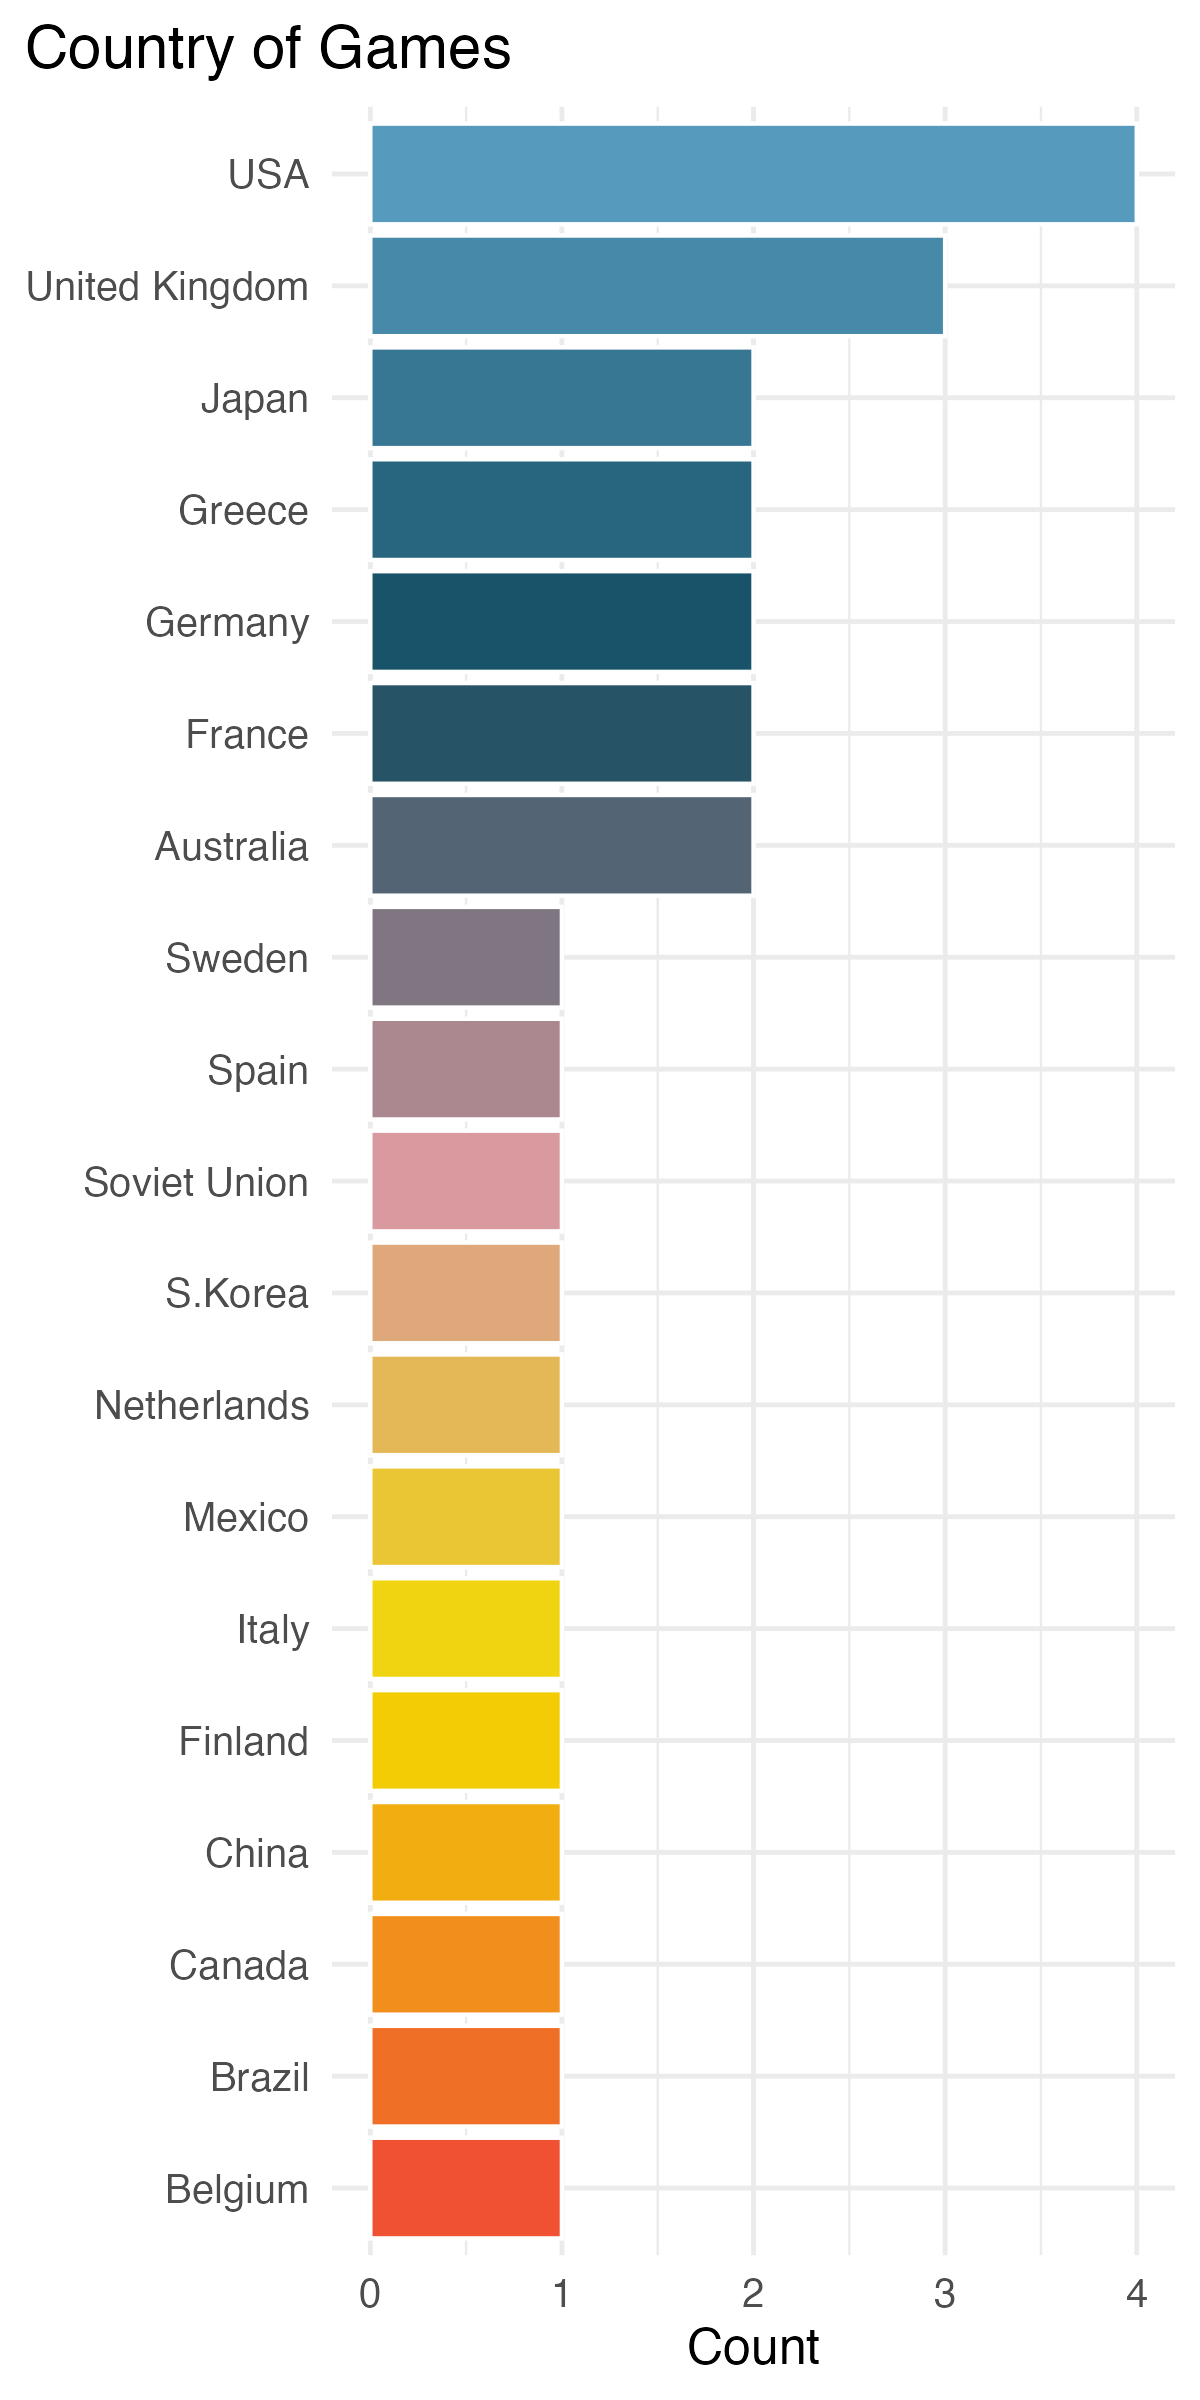
\includegraphics[width=0.8\textwidth,height=\textheight]{03-data-applications_files/figure-pdf/fig-paralympic-cat-1.png}

}

\caption{\label{fig-paralympic-cat}Distributions of categorical
variables in the \texttt{paralympic\_1500} dataset. Plot A shows the
distribution of the country of origin of the athlete; Plot B shows the
distribution of the country in which the Games gook place.}

\end{figure}%

Similarly, we can examine the distributions of the numerical variables
as well. We already know that the 1500m times are mostly between 3.5min
and 4.5min, based on Table~\ref{tbl-paralympic-df-tail} and
Table~\ref{tbl-paralympic-df-head}. We can break down the 1500m time by
division and type of race. Table~\ref{tbl-paralympic-summary} shows the
mean, minimum, and maximum 1500m times broken down by division and race
type. Recall that the Men's Olympic division has taken place since 1896,
whereas the Men's Paralympic division has happened only since 1960. The
maximum race time, therefore, should be taken into context in terms of
the year of the Games.

\clearpage

\begin{table}[H]

\caption{\label{tbl-paralympic-summary}Mean, minimum, and maximum of the
gold medal times for the 1500m race broken down by division and type of
race.}

\centering{

\centering
\begin{tabular}[t]{llrrr}
\toprule
division & type & mean & min & max\\
\midrule
\cellcolor{gray!10}{Men} & \cellcolor{gray!10}{Olympic} & \cellcolor{gray!10}{3.76} & \cellcolor{gray!10}{3.47} & \cellcolor{gray!10}{4.55}\\
Men & T11 & 4.14 & 3.96 & 4.31\\
\cellcolor{gray!10}{Men} & \cellcolor{gray!10}{T12} & \cellcolor{gray!10}{4.11} & \cellcolor{gray!10}{3.94} & \cellcolor{gray!10}{4.25}\\
Men & T13 & 3.98 & 3.81 & 4.24\\
\cellcolor{gray!10}{Women} & \cellcolor{gray!10}{Olympic} & \cellcolor{gray!10}{4.02} & \cellcolor{gray!10}{3.88} & \cellcolor{gray!10}{4.18}\\
Women & T11 & 5.05 & 4.62 & 5.63\\
\cellcolor{gray!10}{Women} & \cellcolor{gray!10}{T12} & \cellcolor{gray!10}{4.88} & \cellcolor{gray!10}{4.61} & \cellcolor{gray!10}{5.57}\\
Women & T13 & 4.55 & 4.23 & 5.24\\
\bottomrule
\end{tabular}

}

\end{table}%

\textbf{Fun fact!} Sometimes playing around with the dataset will
uncover interesting elements about the context in which the data were
collected. A scatterplot of the Men's 1500m broken down by race type
shows that, in each given year, the Olympic runner is substantially
faster than the Paralympic runners, with one exception. In the Rio de
Janeiro 2016 Games, the
\href{https://www.paralympic.org/news/remarkable-finish-1500m-rio-2016}{T13
gold medal athlete ran faster (3:48.29) than the Olympic gold medal
athlete (3:50.00)} (see Figure~\ref{fig-paralympic-rio}). In fact, some
internet sleuthing tells you that the \emph{top four} T13 finishers all
finished the 1500m under 3:50.00!

\begin{figure}[H]

\centering{

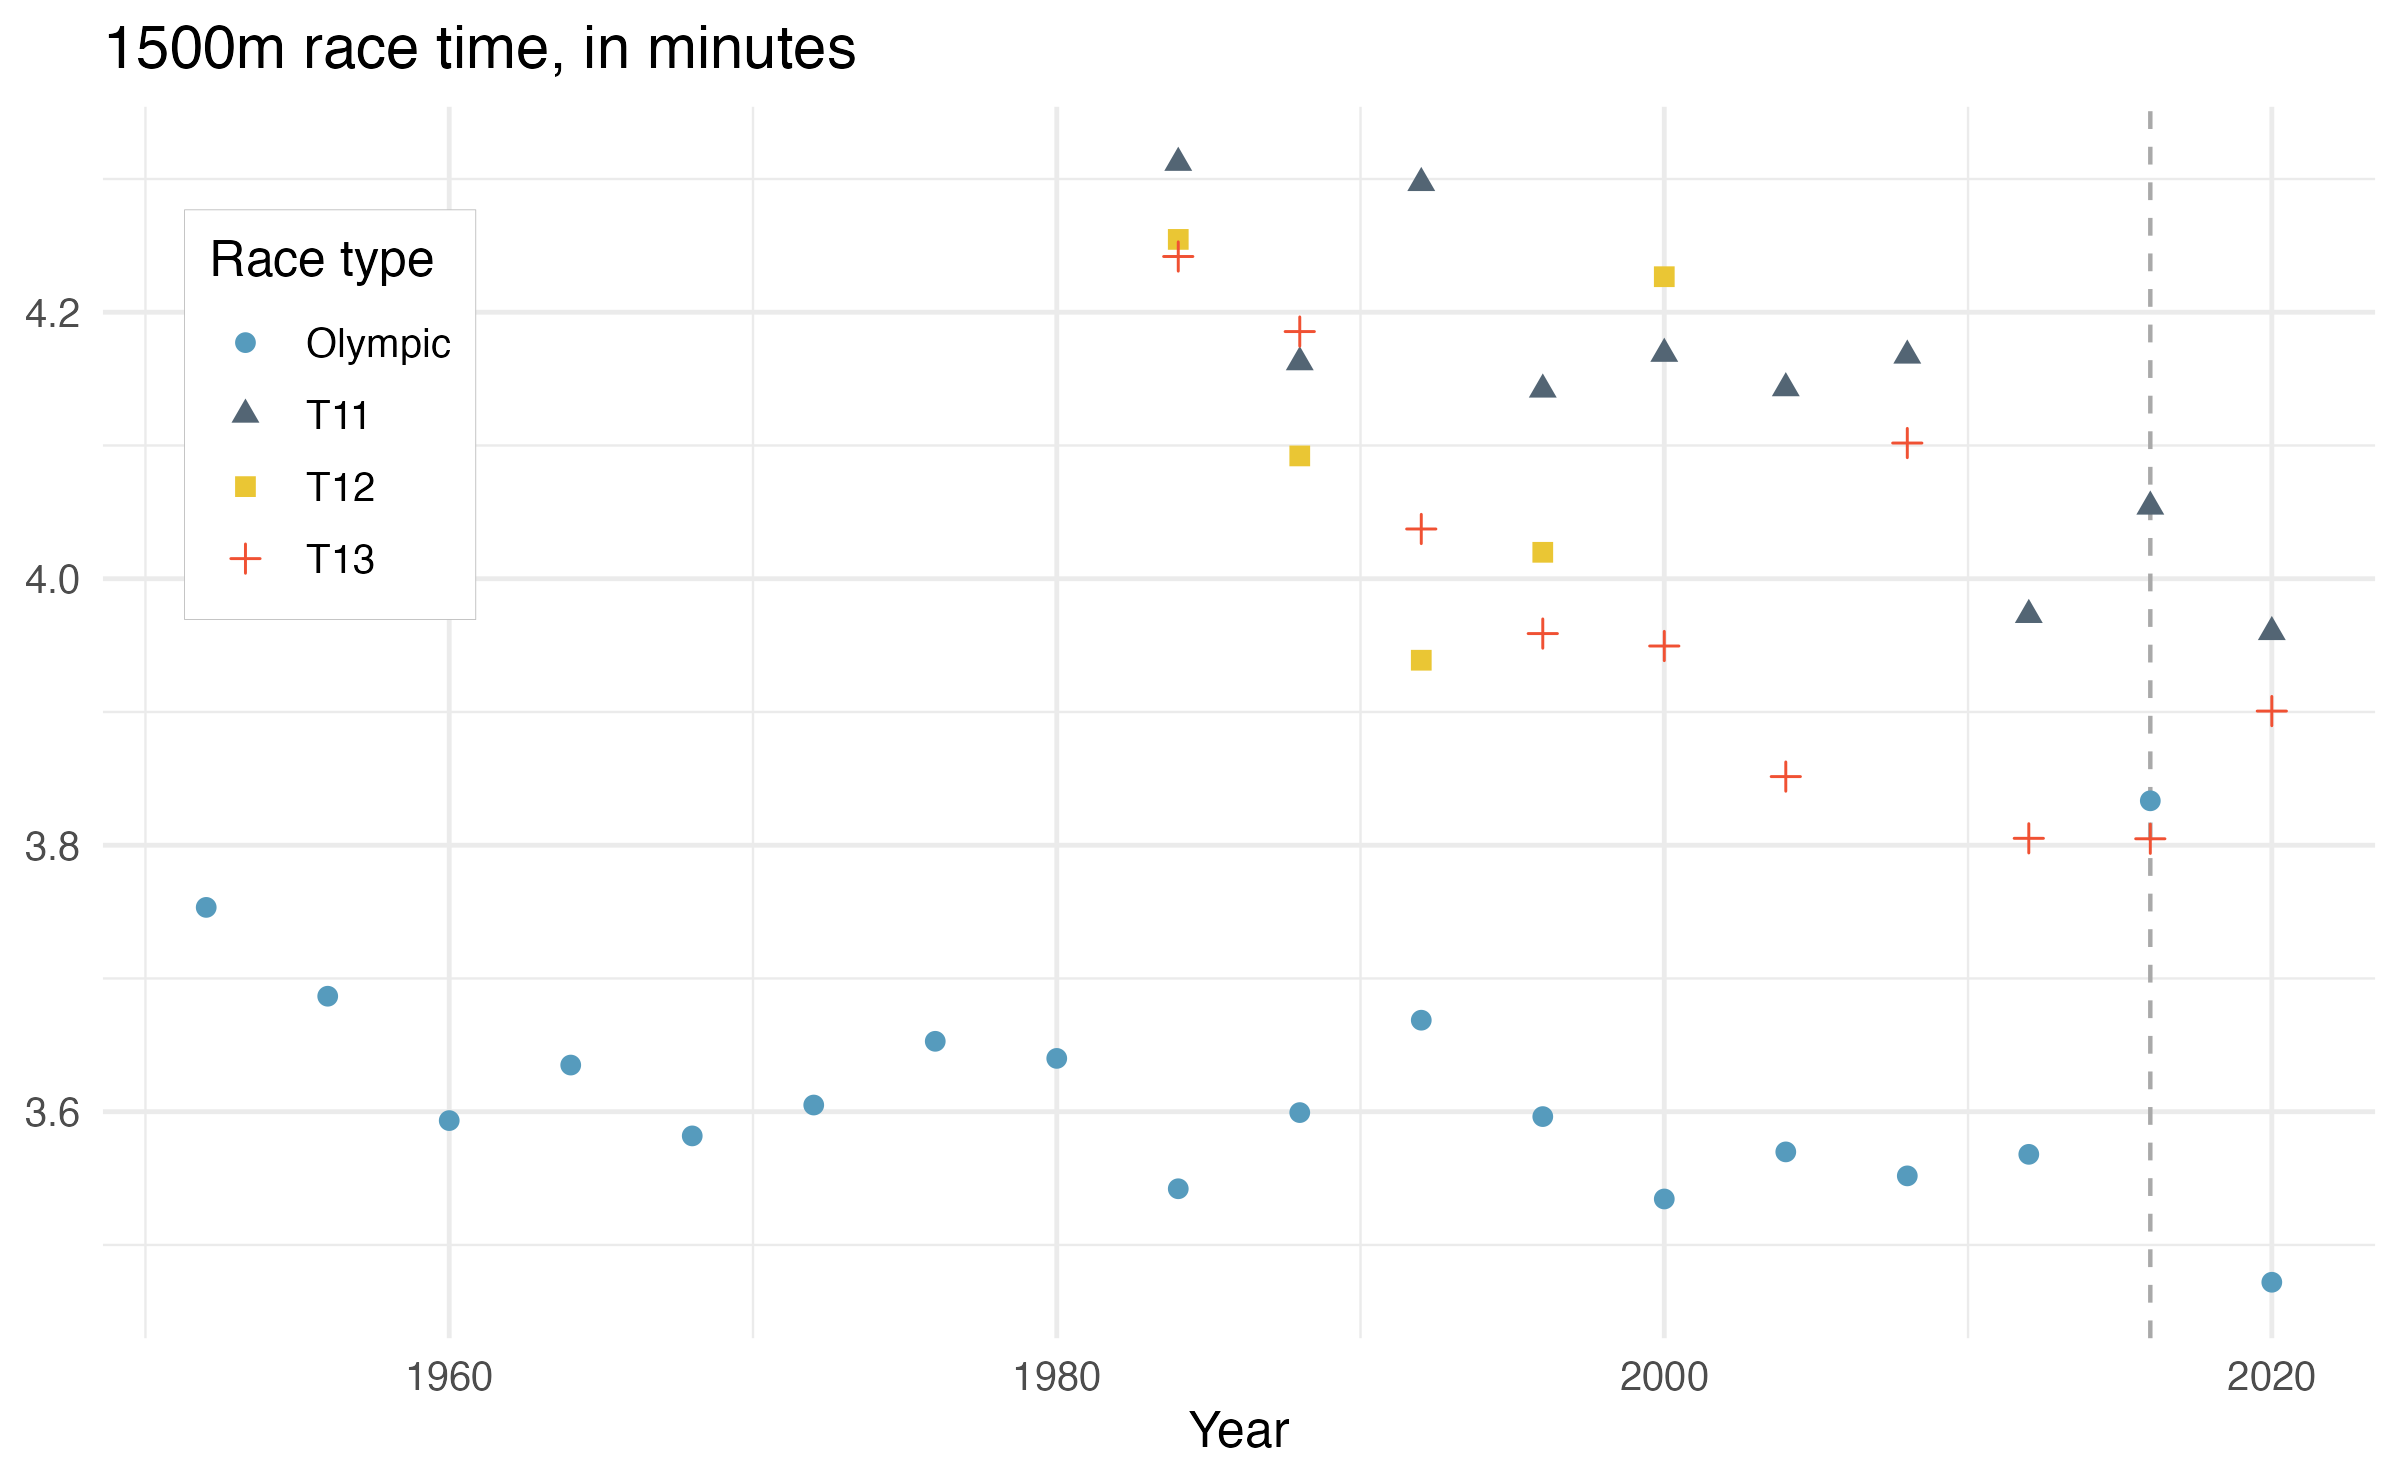
\includegraphics[width=0.8\textwidth,height=\textheight]{03-data-applications_files/figure-pdf/fig-paralympic-rio-1.png}

}

\caption{\label{fig-paralympic-rio}1500m race time for Men's Olympic and
Paralympic athletes. Dashed grey line represents the Rio Games in 2016.}

\end{figure}%

So far we examined aspects of some of the individual variables, and we
have broken down the 1500m race times in terms of division and race
type. You might have already wondered how the race times vary across
year. The \texttt{paralymic\_1500} dataset will provide us with an
ability to explore an important statistical concept, Simpson's paradox.

\clearpage

\section{Simpson's paradox}\label{simpsons-paradox}

Simpson's paradox \index{Simpson's paradox} is a description of three
(or more) variables. The paradox happens when a third variable reverses
the relationship between the first two variables.

Let's start by considering how the 1500m gold medal race times have
changed over year. Figure~\ref{fig-paralympic-ungrouped} shows a
scatterplot describing 1500m race times and year for Men's Olympic and
Paralympic (T11) athletes with a line of best fit (to the entire
dataset) superimposed (see Chapter~\ref{sec-model-slr} where we will
present fitting a line to a scatterplot). Notice that the line of best
fit shows a \emph{positive} relationship between race time and year.
That is, for later years, the predicted gold medal time is higher than
in earlier years.

\begin{figure}[H]

\centering{

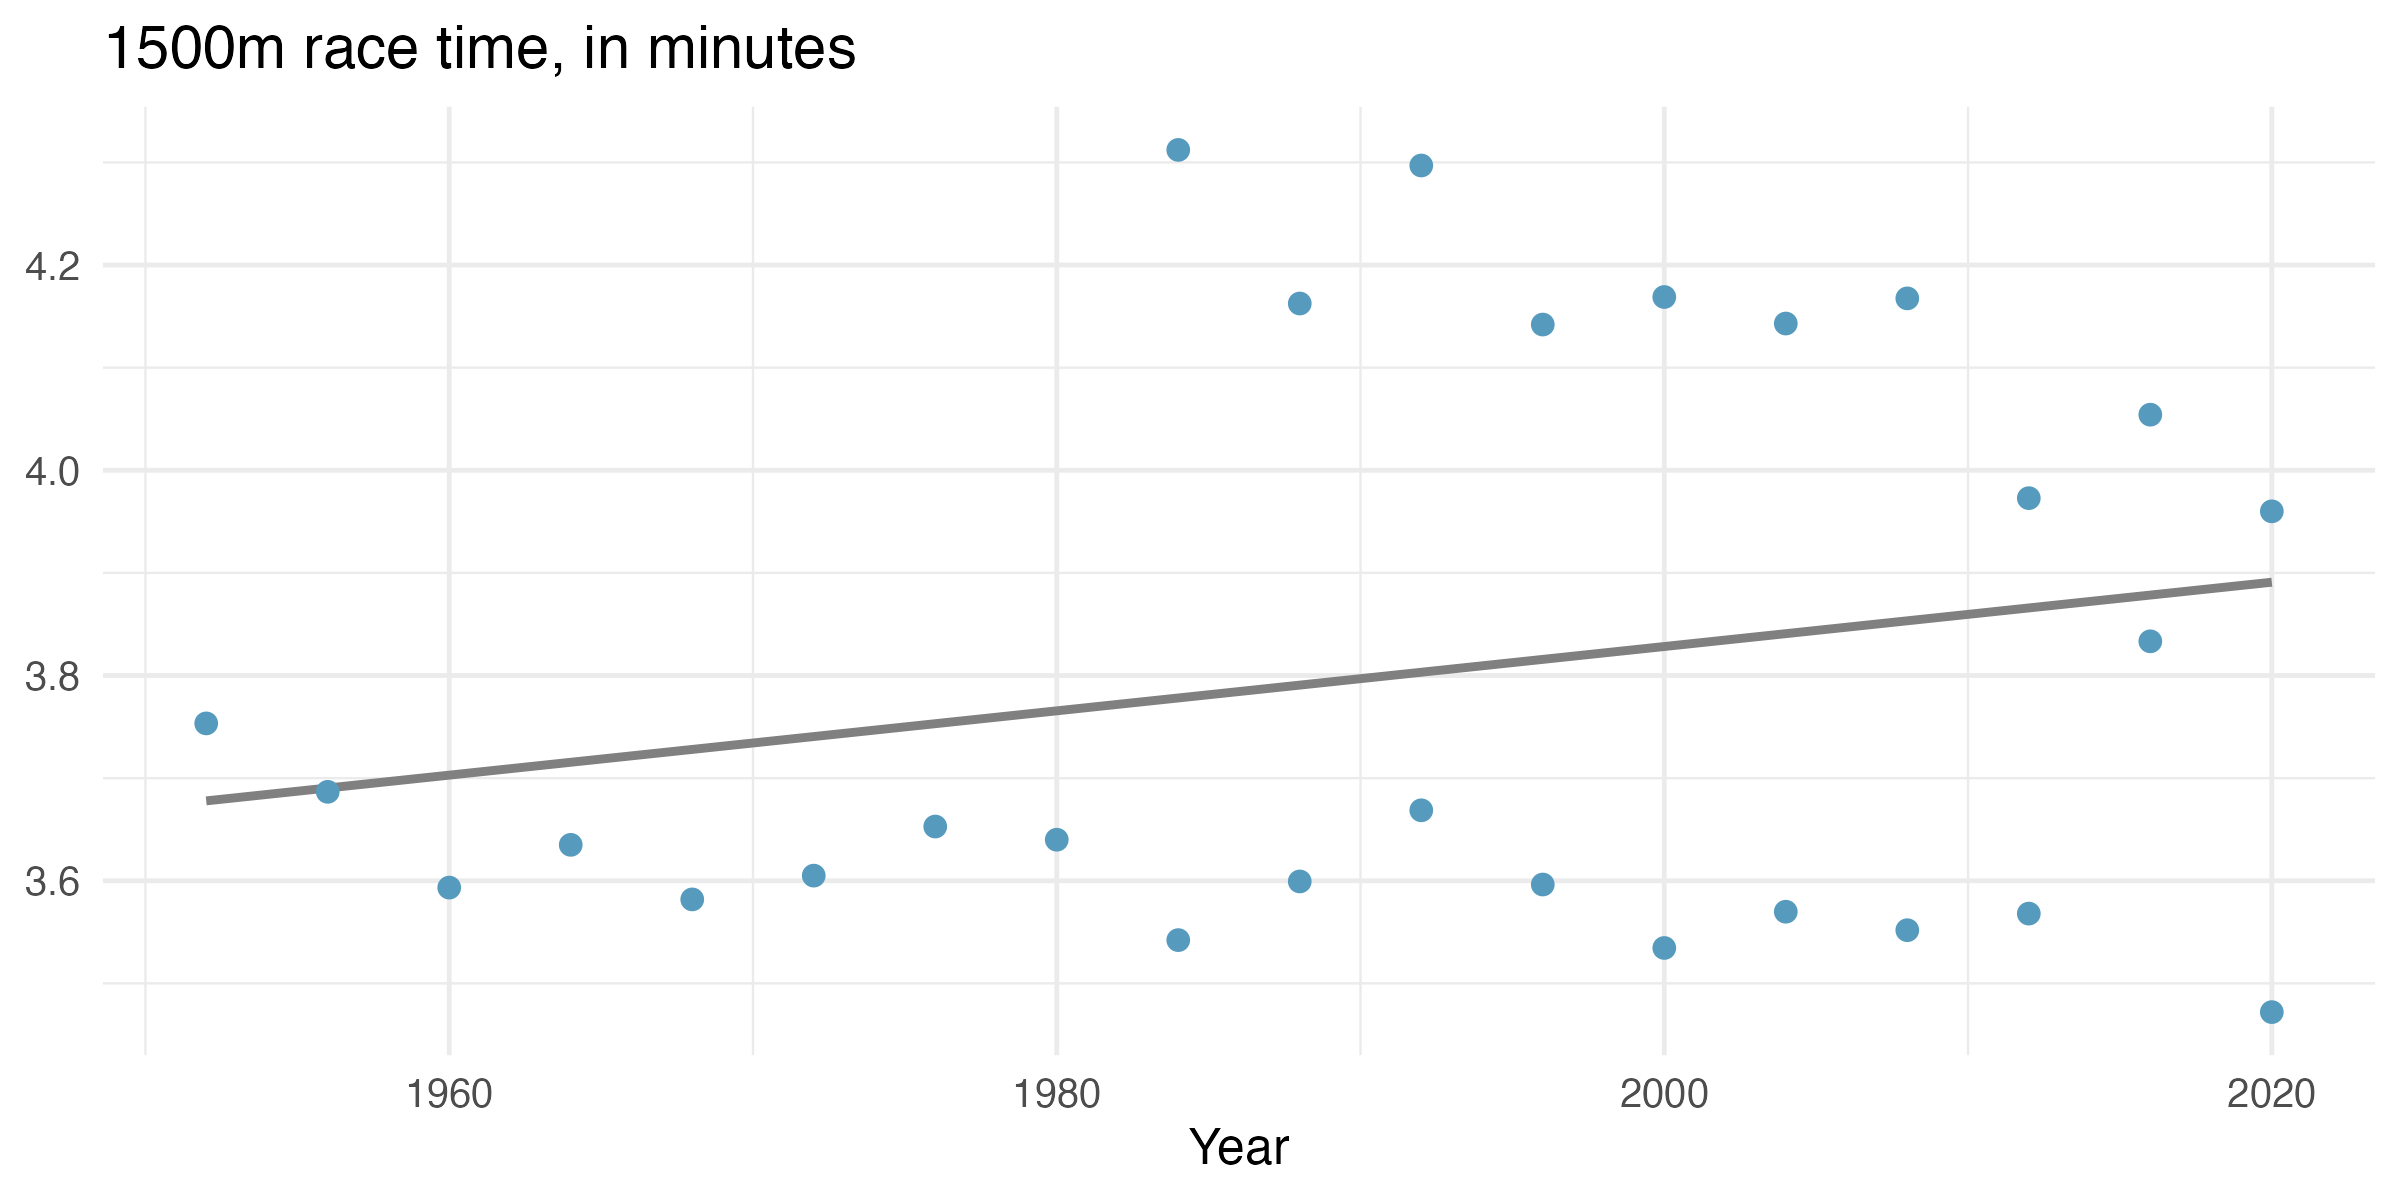
\includegraphics[width=0.8\textwidth,height=\textheight]{03-data-applications_files/figure-pdf/fig-paralympic-ungrouped-1.png}

}

\caption{\label{fig-paralympic-ungrouped}1500m race time for Men's
Olympic and Paralympic (T11) athletes. The line represents a line of
best fit to the entire dataset.}

\end{figure}%

Of course, both your eye and your intuition are likely telling you that
it wouldn't make any sense to try to model all of the athletes together.
Instead, a separate model should be run for each of the two types of
Games: Olympic and Paralympic (T11). Figure~\ref{fig-paralympic-grouped}
shows a scatterplot describing 1500m race times and year for Men's
Olympic and Paralympic (T11) athletes with a line of best fit
superimposed separately for each of the two types of races. Notice that
within each type of race, the relationship between 1500m race time and
year is now \emph{negative}.

\begin{figure}[H]

\centering{

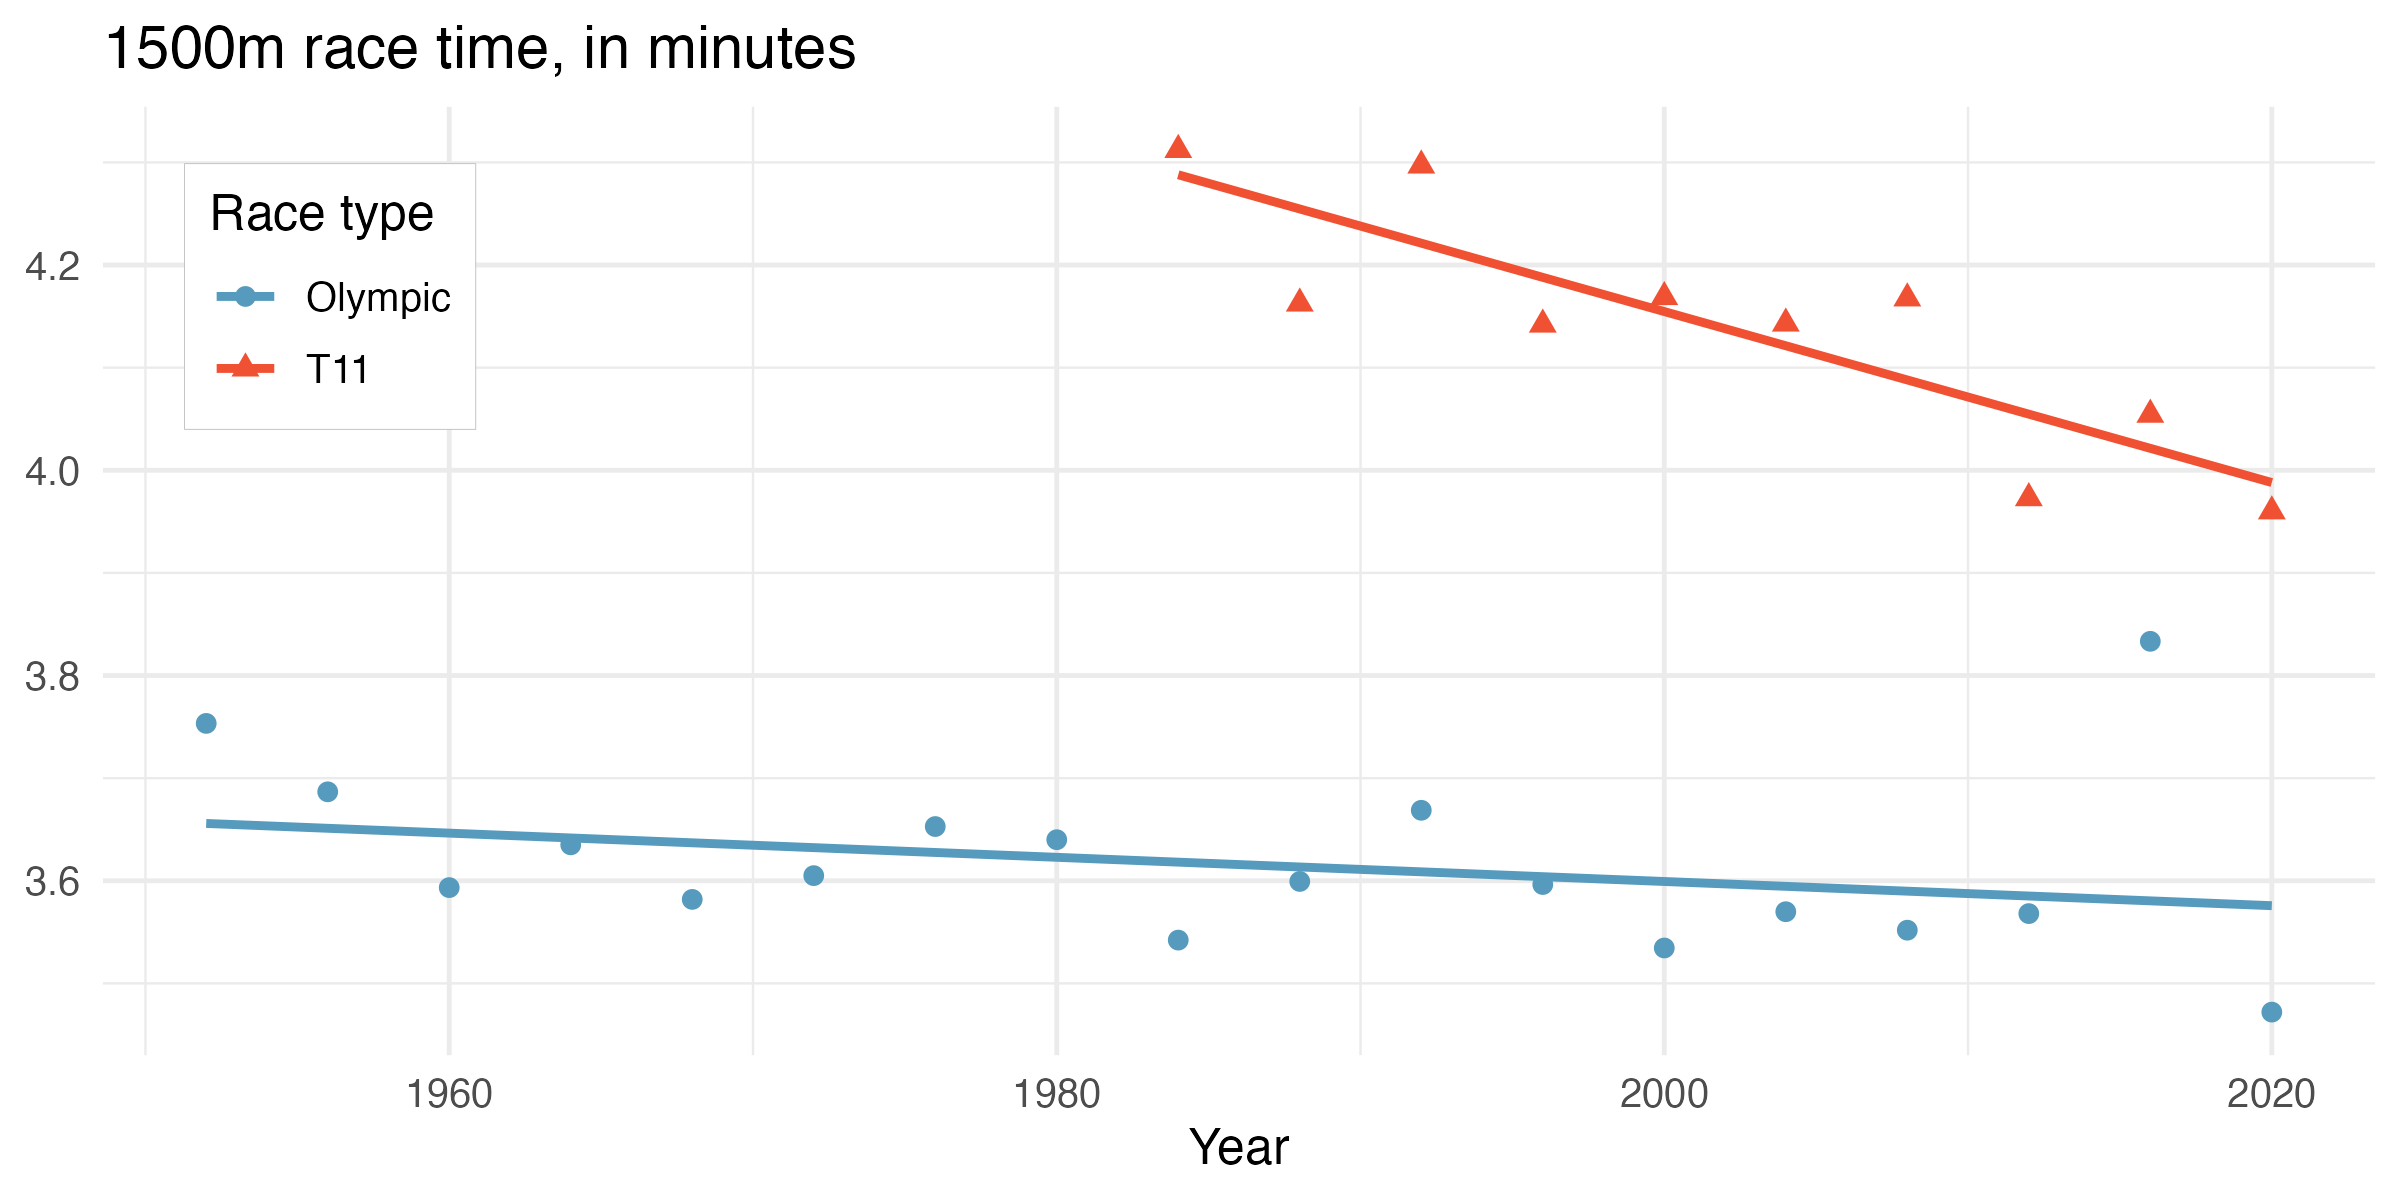
\includegraphics[width=0.8\textwidth,height=\textheight]{03-data-applications_files/figure-pdf/fig-paralympic-grouped-1.png}

}

\caption{\label{fig-paralympic-grouped}1500m race time for Men's Olympic
and Paralympic (T11) athletes. The best fit line is now fit separately
to the Olympic and Paralympic athletes.}

\end{figure}%

\begin{important}
\textbf{Simpson's paradox.}

Simpson's paradox happens when an association or relationship between
two variables in one direction (e.g., positive) reverses (e.g., becomes
negative) when a third variable is considered.

\end{important}

Simpson's paradox was seen in the 1500m race data because the aggregate
data showed a positive relationship (positive slope) between year and
race time but a negative relationship (negative slope) between year and
race time when broken down by the type of race.

Simpson's paradox is observed with categorical data and with numeric
data. Often the paradox happens because the third variable (here, race
type) is imbalanced. There are either more observations in one group or
the observations happen at different intervals across the two groups. In
the 1500m data, we saw that the T11 runners had fewer observations and
their times were both generally slower and more recent than the Olympic
runners.

In the 1500m analysis, it would be most prudent to report the trends
separately for the Olympic and the T11 athletes. However, in other
situations, it might be better to aggregate the data and report the
overall trend. Many additional examples of Simpson's paradox and a
further exploration is given in Witmer (2021).

In this case study, we introduced you to the very first steps a data
scientist takes when they start working with a new dataset. In the next
few chapters, we will introduce exploratory data analysis, and you'll
learn more about the various types of data visualizations and summary
statistics you can make to get to know your data better.

Before you move on, we encourage you to think about whether the
following questions can be answered with this dataset, and if yes, how
you might go about answering them? It's okay if your answer is ``I'm not
sure'', we simply want to get your exploratory juices flowing to prime
you for what's to come!

\begin{enumerate}
\def\labelenumi{\arabic{enumi}.}
\tightlist
\item
  Has there every been a year when a visually impaired paralympic gold
  medal athlete beat the Olympic gold medal athlete?
\item
  When comparing the paralympic and Olympic 1500m gold medal athletes,
  does Simpson's paradox hold in the Women's division?
\item
  Is there a biological boundary which establishes a time under which no
  human could run 1500m?
\end{enumerate}

\clearpage

\section{Interactive R tutorials}\label{sec-data-tutorials}

Navigate the concepts you've learned in this chapter in R using the
following self-paced tutorials. All you need is your browser to get
started!

\begin{alltutorials}

\href{https://openintrostat.github.io/ims-tutorials/01-data/}{Tutorial
1: Introduction to data}

\url{https://openintrostat.github.io/ims-tutorials/01-data}

\end{alltutorials}

\begin{singletutorial}

\href{https://openintro.shinyapps.io/ims-01-data-01/}{Tutorial 1 -
Lesson 1: Language of data}

\url{https://openintro.shinyapps.io/ims-01-data-01}

\end{singletutorial}

\begin{singletutorial}

\href{https://openintro.shinyapps.io/ims-01-data-02/}{Tutorial 1 -
Lesson 2: Types of studies}

\url{https://openintro.shinyapps.io/ims-01-data-02}

\end{singletutorial}

\begin{singletutorial}

\href{https://openintro.shinyapps.io/ims-01-data-03/}{Tutorial 1 -
Lesson 3: Sampling strategies and experimental design}

\url{https://openintro.shinyapps.io/ims-01-data-03}

\end{singletutorial}

\begin{singletutorial}

\href{https://openintro.shinyapps.io/ims-01-data-04/}{Tutorial 1 -
Lesson 4: Case study}

\url{https://openintro.shinyapps.io/ims-01-data-04}

\end{singletutorial}

You can also access the full list of tutorials supporting this book at\\
\url{https://openintrostat.github.io/ims-tutorials}.

\section{R labs}\label{sec-data-labs}

Further apply the concepts you've learned in this part in R with
computational labs that walk you through a data analysis case study.

\begin{singlelab}

\href{https://www.openintro.org/go?id=ims-r-lab-intro-to-r}{Intro to R -
Birth rates}

\url{https://www.openintro.org/go?id=ims-r-lab-intro-to-r}

\end{singlelab}

You can also access the full list of labs supporting this book at\\
\url{https://www.openintro.org/go?id=ims-r-labs}.

\part{Exploratory data analysis}

After obtaining a dataset, it is vitally important to understand the
characteristics of the existing data. Sometimes the most effective way
to grasp the data is through summary statistics or other numerical
measures. Often, however, it is a picture that tells a thousand words.
Knowing how to best convey the underlying meaning in a dataset is a
hugely important aspect of communicating results.

\begin{itemize}
\tightlist
\item
  Categorical data is the focus of
  Chapter~\ref{sec-explore-categorical}. Both numerical and graphical
  summaries are presented as ways to convey information about
  categorical data.
\item
  Numerical data is the focus of Chapter~\ref{sec-explore-numerical}.
  Both numerical and graphical summaries are presented as ways to convey
  information about numerical data.
\item
  Chapter~\ref{sec-explore-applications} does a deep dive into important
  considerations when creating a visualization.
\end{itemize}

While our book is software agnostic, one of the best ways to become
familiar with numerical and graphical summaries is to practice working
with different datasets using statistical software. For example, if you
are interested in using R, you might try working through some of the
chapters in \href{https://r4ds.hadley.nz/}{R for Data Science}
(https://r4ds.hadley.nz), specifically the parts
\href{https://r4ds.hadley.nz/whole-game}{Whole game} and
\href{https://r4ds.hadley.nz/visualize}{Visualize}.

\chapter{Exploring categorical data}\label{sec-explore-categorical}

\begin{chapterintro}
This chapter focuses on exploring \textbf{categorical} data using
summary statistics and visualizations. The summaries and graphs
presented in this chapter are created using statistical software;
however, since this might be your first exposure to the concepts, we
take our time in this chapter to detail how to create them. Where
possible, we present multivariate plots; plots that visualize the
relationship between multiple variables. Mastery of the content
presented in this chapter will be crucial for understanding the methods
and techniques introduced in the rest of the book.

\end{chapterintro}

In this chapter we will work with data on loans from Lending Club that
you've previously seen in Chapter~\ref{sec-data-hello}. The
\texttt{loan50} dataset from Chapter~\ref{sec-data-hello} represents a
sample from a larger loan dataset called \texttt{loans}. This larger
dataset contains information on 10,000 loans made through Lending Club.
We will examine the relationship between \texttt{homeownership}, which
for the \texttt{loans} data can take a value of \texttt{rent},
\texttt{mortgage} (owns but has a mortgage), or \texttt{own}, and
\texttt{app\_type}, which indicates whether the loan application was
made with a partner or whether it was an individual application.

\begin{data}
The
\href{http://openintrostat.github.io/openintro/reference/loans_full_schema.html}{\texttt{loans\_full\_schema}}
data can be found in the
\href{http://openintrostat.github.io/openintro}{\textbf{openintro}} R
package. Based on the data in this dataset we have modified the
\texttt{homeownership} and \texttt{application\_type} variables. We will
refer to this modified dataset as \texttt{loans}.

\end{data}

\section{Contingency tables and bar
plots}\label{contingency-tables-and-bar-plots}

Table~\ref{tbl-loan-home-app-type-totals} summarizes two variables:
\texttt{application\_type} and \texttt{homeownership}. Note that loans
from Lending Club are typically for small items or for cash, not for
homes. The individuals in the dataset are taking out loans for their
personal use, and we categorize them based on their
\texttt{homeownership} status (which is unrelated to the purpose of the
loan). A table that summarizes data for two categorical variables in
this way is called a \textbf{contingency table}. Each value in the table
represents the number of times a particular combination of variable
outcomes occurred.

For example, the value 3496 corresponds to the number of loans in the
dataset where the borrower rents their home and the application type was
by an individual. Row and column totals are also included. The
\textbf{row totals} provide the total counts across each row and the
\textbf{column totals} down each column. We can also create a table that
shows only the overall percentages or proportions for each combination
of categories, or we can create a table for a single variable, such as
the one shown in Table~\ref{tbl-loan-homeownership-totals} for the
\texttt{homeownership} variable.

\begin{table}[H]

\caption{\label{tbl-loan-home-app-type-totals}A contingency table for
application type and homeownership.}

\centering{

\centering
\begin{tabular}[t]{>{\raggedright\arraybackslash}p{8em}>{\raggedleft\arraybackslash}p{5em}>{\raggedleft\arraybackslash}p{5em}>{\raggedleft\arraybackslash}p{5em}>{\raggedleft\arraybackslash}p{5em}}
\toprule
\multicolumn{1}{c}{ } & \multicolumn{3}{c}{homeownership} & \multicolumn{1}{c}{ } \\
\cmidrule(l{3pt}r{3pt}){2-4}
application\_type & rent & mortgage & own & Total\\
\midrule
\cellcolor{gray!10}{joint} & \cellcolor{gray!10}{362} & \cellcolor{gray!10}{950} & \cellcolor{gray!10}{183} & \cellcolor{gray!10}{1495}\\
individual & 3496 & 3839 & 1170 & 8505\\
\cellcolor{gray!10}{Total} & \cellcolor{gray!10}{3858} & \cellcolor{gray!10}{4789} & \cellcolor{gray!10}{1353} & \cellcolor{gray!10}{10000}\\
\bottomrule
\end{tabular}

}

\end{table}%

\begin{table}[H]

\caption{\label{tbl-loan-homeownership-totals}A table summarizing the
frequencies for each value of the homeownership variable -- mortgage,
own, and rent.}

\centering{

\centering
\begin{tabular}[t]{>{\raggedright\arraybackslash}p{10em}>{\raggedleft\arraybackslash}p{10em}}
\toprule
homeownership & Count\\
\midrule
\cellcolor{gray!10}{rent} & \cellcolor{gray!10}{3858}\\
mortgage & 4789\\
\cellcolor{gray!10}{own} & \cellcolor{gray!10}{1353}\\
Total & 10000\\
\bottomrule
\end{tabular}

}

\end{table}%

A bar plot is a common way to display a single categorical variable.
Figure~\ref{fig-loan-homeownership-bar-plot-1} displays a \textbf{bar
plot} of the \texttt{homeownership} variable. In
Figure~\ref{fig-loan-homeownership-bar-plot-2} the counts are converted
into proportions, showing the proportion of observations that are in
each level.

\begin{figure}[H]

\begin{minipage}{0.50\linewidth}

\centering{

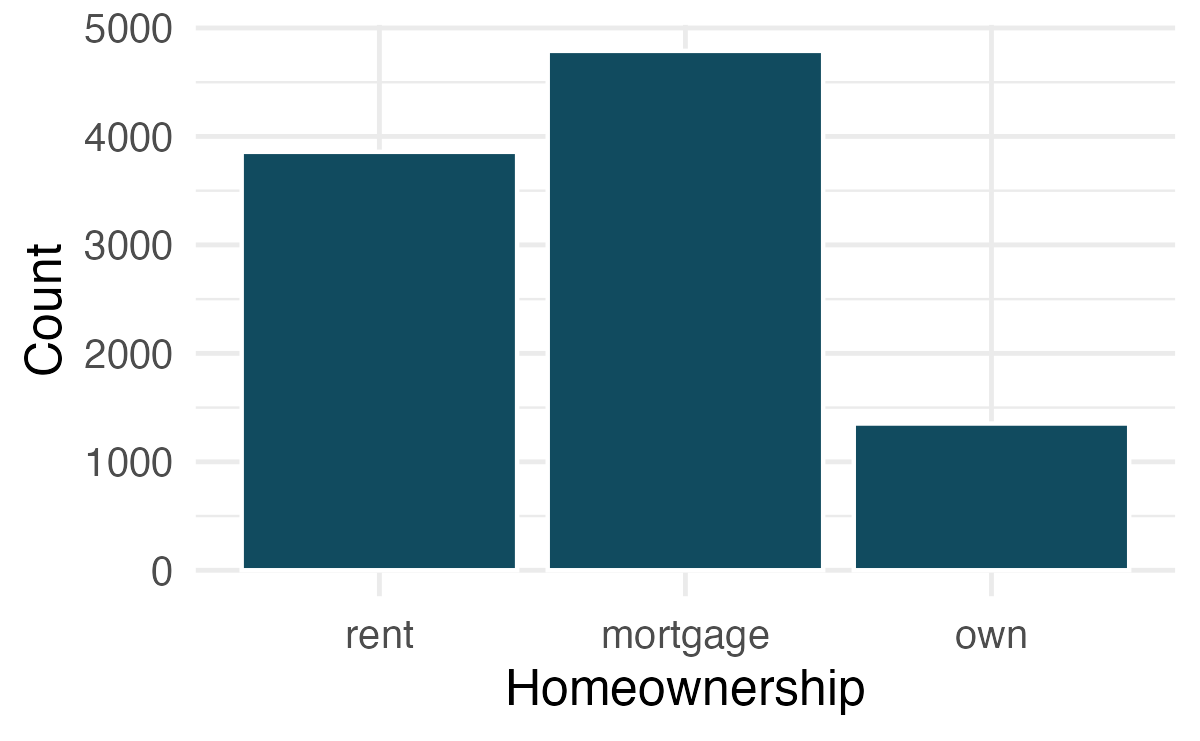
\includegraphics[width=0.8\textwidth,height=\textheight]{04-explore-categorical_files/figure-pdf/fig-loan-homeownership-bar-plot-1.png}

}

\subcaption{\label{fig-loan-homeownership-bar-plot-1}Counts of
homeownership.}

\end{minipage}%
%
\begin{minipage}{0.50\linewidth}

\centering{

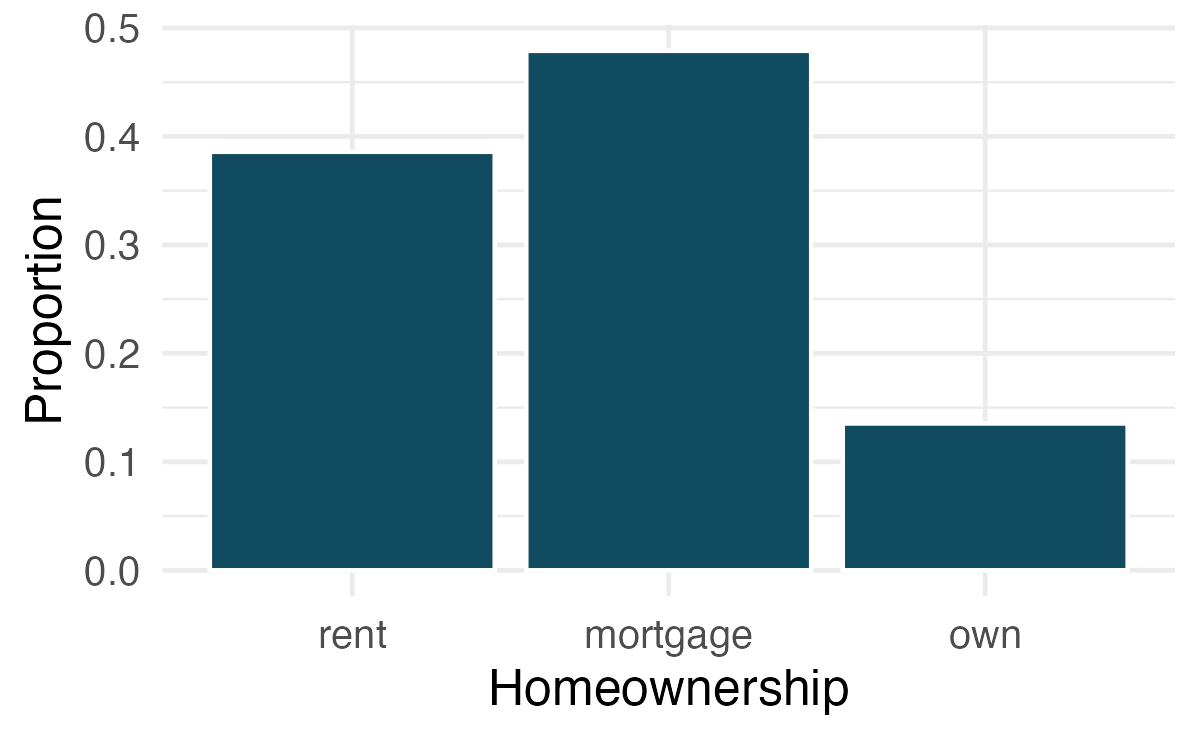
\includegraphics[width=0.8\textwidth,height=\textheight]{04-explore-categorical_files/figure-pdf/fig-loan-homeownership-bar-plot-2.png}

}

\subcaption{\label{fig-loan-homeownership-bar-plot-2}Proportions of
homeownership.}

\end{minipage}%

\caption{\label{fig-loan-homeownership-bar-plot}Distribution of
homeownership.}

\end{figure}%

\section{Visualizing two categorical
variables}\label{visualizing-two-categorical-variables}

\subsection{Bar plots with two
variables}\label{bar-plots-with-two-variables}

We can display the distributions of two categorical variables on a bar
plot concurrently. Such plots are generally useful for visualizing the
relationship between two categorical variables.
Figure~\ref{fig-loan-homeownership-app-type-bar-plot} shows three such
plots that visualize
Figure~\ref{fig-loan-homeownership-app-type-bar-plot-1} is a
\textbf{stacked bar plot}. This plot most clearly displays that loan
applicants most commonly live in mortgaged homes. It is difficult to
say, based on this plot alone, how different application types vary
across the levels of homeownership.
Figure~\ref{fig-loan-homeownership-app-type-bar-plot-2} is a
\textbf{standardized bar plot} (also known as \textbf{filled bar plot}).
This type of visualization is helpful in understanding the fraction of
individual or joint loan applications for borrowers in each level of
\texttt{homeownership}. Additionally, since the proportions of joint and
individual loans vary across the groups, we can conclude that the two
variables are associated for this sample. Finally,
Figure~\ref{fig-loan-homeownership-app-type-bar-plot-3} is a
\textbf{dodged bar plot}. This plot most clearly displays that within
each level of homeownership, individual applications are more common
than joint applications. This plot most clearly displays that joint
applications are most common among loans for applicants who live in
mortgaged homes, compared to renters and owners.

\begin{figure}[H]

\begin{minipage}{0.50\linewidth}

\centering{

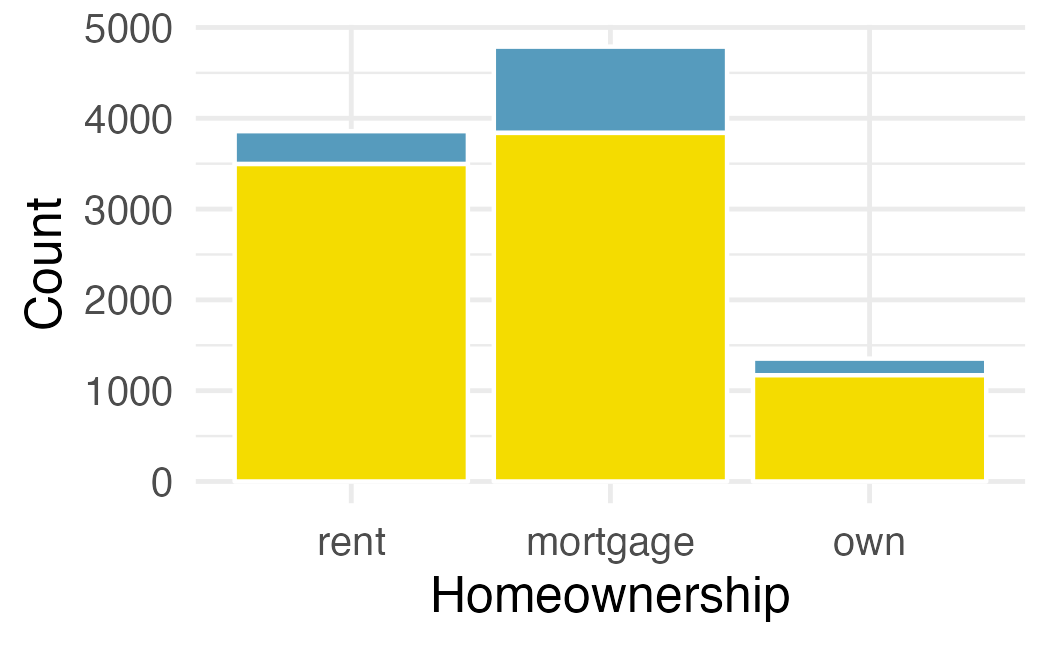
\includegraphics[width=0.8\textwidth,height=\textheight]{04-explore-categorical_files/figure-pdf/fig-loan-homeownership-app-type-bar-plot-1.png}

}

\subcaption{\label{fig-loan-homeownership-app-type-bar-plot-1}Stacked
bar plot}

\end{minipage}%
%
\begin{minipage}{0.50\linewidth}

\centering{

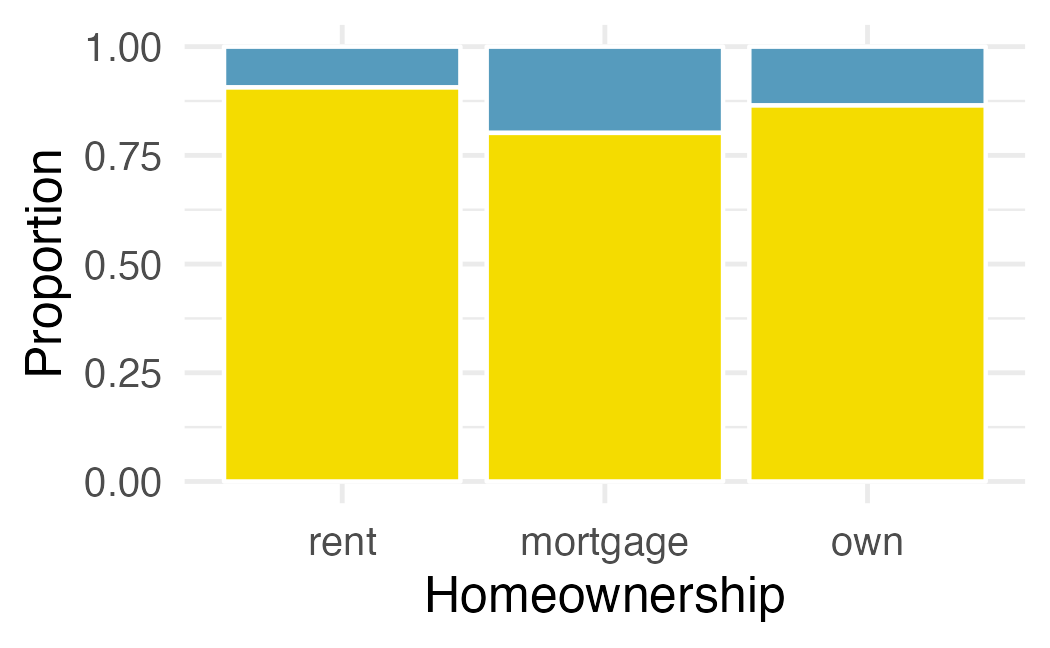
\includegraphics[width=0.8\textwidth,height=\textheight]{04-explore-categorical_files/figure-pdf/fig-loan-homeownership-app-type-bar-plot-2.png}

}

\subcaption{\label{fig-loan-homeownership-app-type-bar-plot-2}Standardized
bar plot}

\end{minipage}%
\newline
\begin{minipage}{0.22\linewidth}
~\end{minipage}%
%
\begin{minipage}{0.56\linewidth}

\centering{

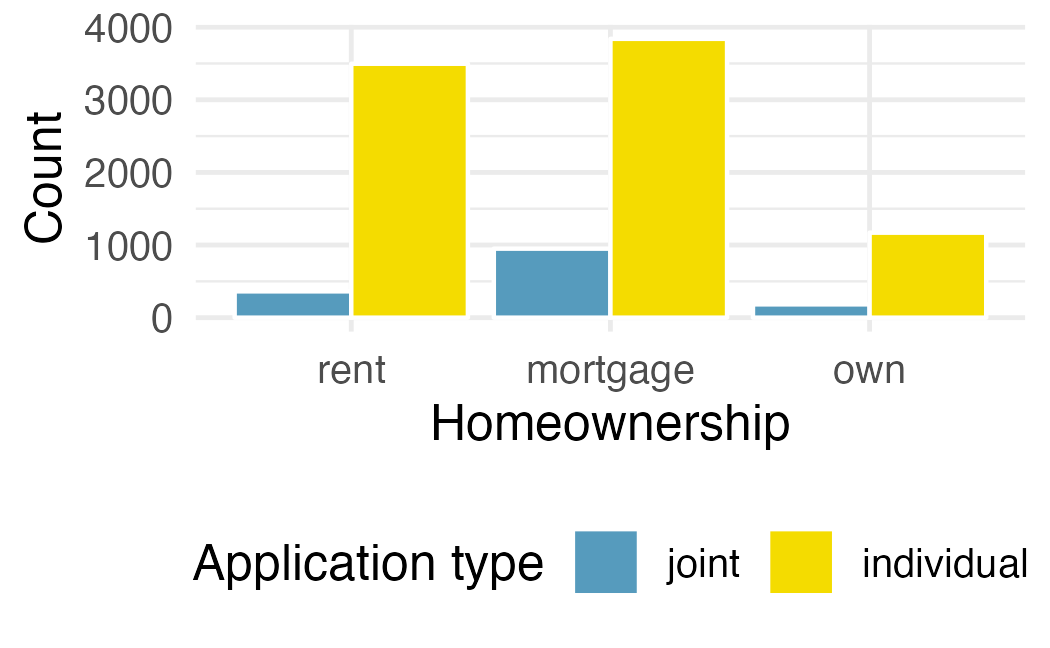
\includegraphics[width=0.8\textwidth,height=\textheight]{04-explore-categorical_files/figure-pdf/fig-loan-homeownership-app-type-bar-plot-3.png}

}

\subcaption{\label{fig-loan-homeownership-app-type-bar-plot-3}Dodged bar
plot}

\end{minipage}%
%
\begin{minipage}{0.22\linewidth}
~\end{minipage}%

\caption{\label{fig-loan-homeownership-app-type-bar-plot}Three bar plots
displaying homeownership and application type variables.}

\end{figure}%

\begin{workedexample}
Examine the three bar plots in
Figure~\ref{fig-loan-homeownership-app-type-bar-plot}. When is the
stacked, dodged, or standardized bar plot the most useful?

\begin{center}\rule{0.5\linewidth}{0.5pt}\end{center}

The stacked bar plot is most useful when it's reasonable to assign one
variable as the explanatory variable (here \texttt{homeownership}) and
the other variable as the response (here \texttt{application\_type})
since we are effectively grouping by one variable first and then
breaking it down by the others.

Dodged bar plots are more agnostic in their display about which
variable, if any, represents the explanatory and which the response
variable. It is also easy to discern the number of cases in each of the
six different group combinations. However, one downside is that it tends
to require more horizontal space; the narrowness of Plot B compared to
the other two in Figure~\ref{fig-loan-homeownership-app-type-bar-plot}
makes the plot feel a bit cramped. Additionally, when two groups are of
very different sizes, as we see in the group \texttt{own} relative to
either of the other two groups, it is difficult to discern if there is
an association between the variables.

The standardized stacked bar plot is helpful if the primary variable in
the stacked bar plot is relatively imbalanced, e.g., the category has
only a third of the observations in the category, making the simple
stacked bar plot less useful for checking for an association. The major
downside of the standardized version is that we lose all sense of how
many cases each of the bars represents.

\end{workedexample}

\subsection{Mosaic plots}\label{mosaic-plots}

A \textbf{mosaic plot} is a visualization technique suitable for
contingency tables that resembles a standardized stacked bar plot with
the benefit that we still see the relative group sizes of the primary
variable as well.

To get started in creating our first mosaic plot, we'll break a square
into columns for each category of the variable, with the result shown in
Figure~\ref{fig-loan-homeownership-type-mosaic-plot-1}. Each column
represents a level of \texttt{homeownership}, and the column widths
correspond to the proportion of loans in each of those categories. For
instance, there are fewer loans where the borrower is an owner than
where the borrower has a mortgage. In general, mosaic plots use box
\emph{areas} to represent the number of cases in each category.

Figure~\ref{fig-loan-homeownership-type-mosaic-plot-2} displays the
relationship between homeownership and application type. Each column is
split proportionally to the number of loans from individual and joint
borrowers. For example, the second column represents loans where the
borrower has a mortgage, and it was divided into individual loans
(upper) and joint loans (lower). As another example, the bottom segment
of the third column represents loans where the borrower owns their home
and applied jointly, while the upper segment of this column represents
borrowers who are homeowners and filed individually. We can again use
this plot to see that the \texttt{homeownership} and
\texttt{application\_type} variables are associated, since some columns
are divided in different vertical locations than others, which was the
same technique used for checking an association in the standardized
stacked bar plot.

\begin{figure}[H]

\begin{minipage}{0.50\linewidth}

\centering{

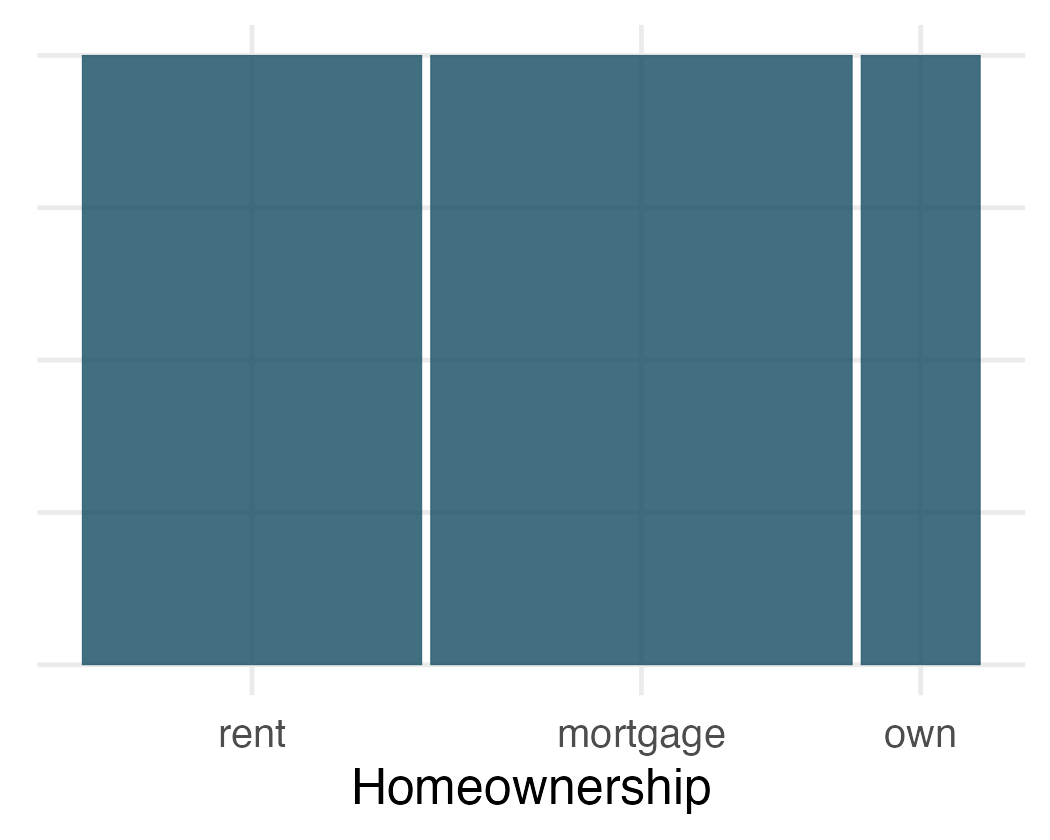
\includegraphics[width=0.8\textwidth,height=\textheight]{04-explore-categorical_files/figure-pdf/fig-loan-homeownership-type-mosaic-plot-1.png}

}

\subcaption{\label{fig-loan-homeownership-type-mosaic-plot-1}Homeownership.}

\end{minipage}%
%
\begin{minipage}{0.50\linewidth}

\centering{

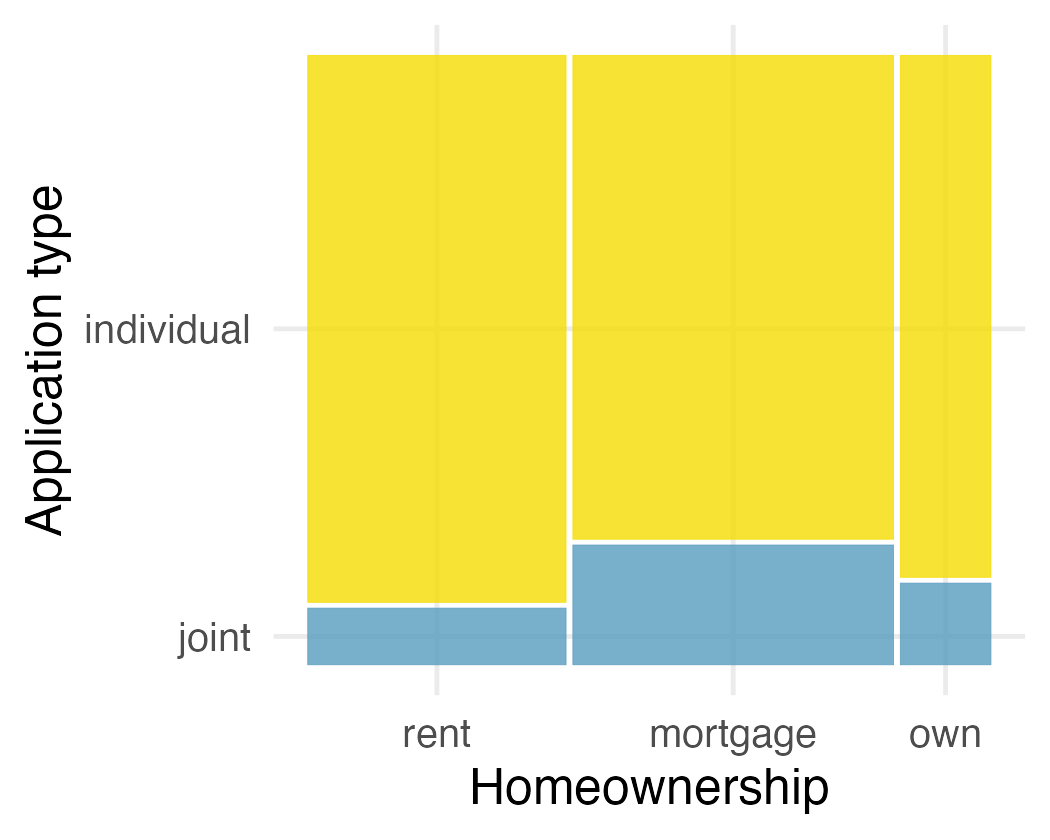
\includegraphics[width=0.8\textwidth,height=\textheight]{04-explore-categorical_files/figure-pdf/fig-loan-homeownership-type-mosaic-plot-2.png}

}

\subcaption{\label{fig-loan-homeownership-type-mosaic-plot-2}Homeownership
vs.~application type.}

\end{minipage}%

\caption{\label{fig-loan-homeownership-type-mosaic-plot}Two mosaic
plots, one for homeownership alone and the other displaying the
relationship between homeownership and application type.}

\end{figure}%

In Figure~\ref{fig-loan-homeownership-type-mosaic-plot}, we chose to
first split by the homeowner status of the borrower. However, we could
have instead first split by the application type, as in
Figure~\ref{fig-loan-app-type-mosaic-plot}. Like with the bar plots,
it's common to use the explanatory variable to represent the first split
in a mosaic plot, and then for the response to break up each level of
the explanatory variable if these labels are reasonable to attach to the
variables under consideration.

\begin{figure}[H]

\centering{

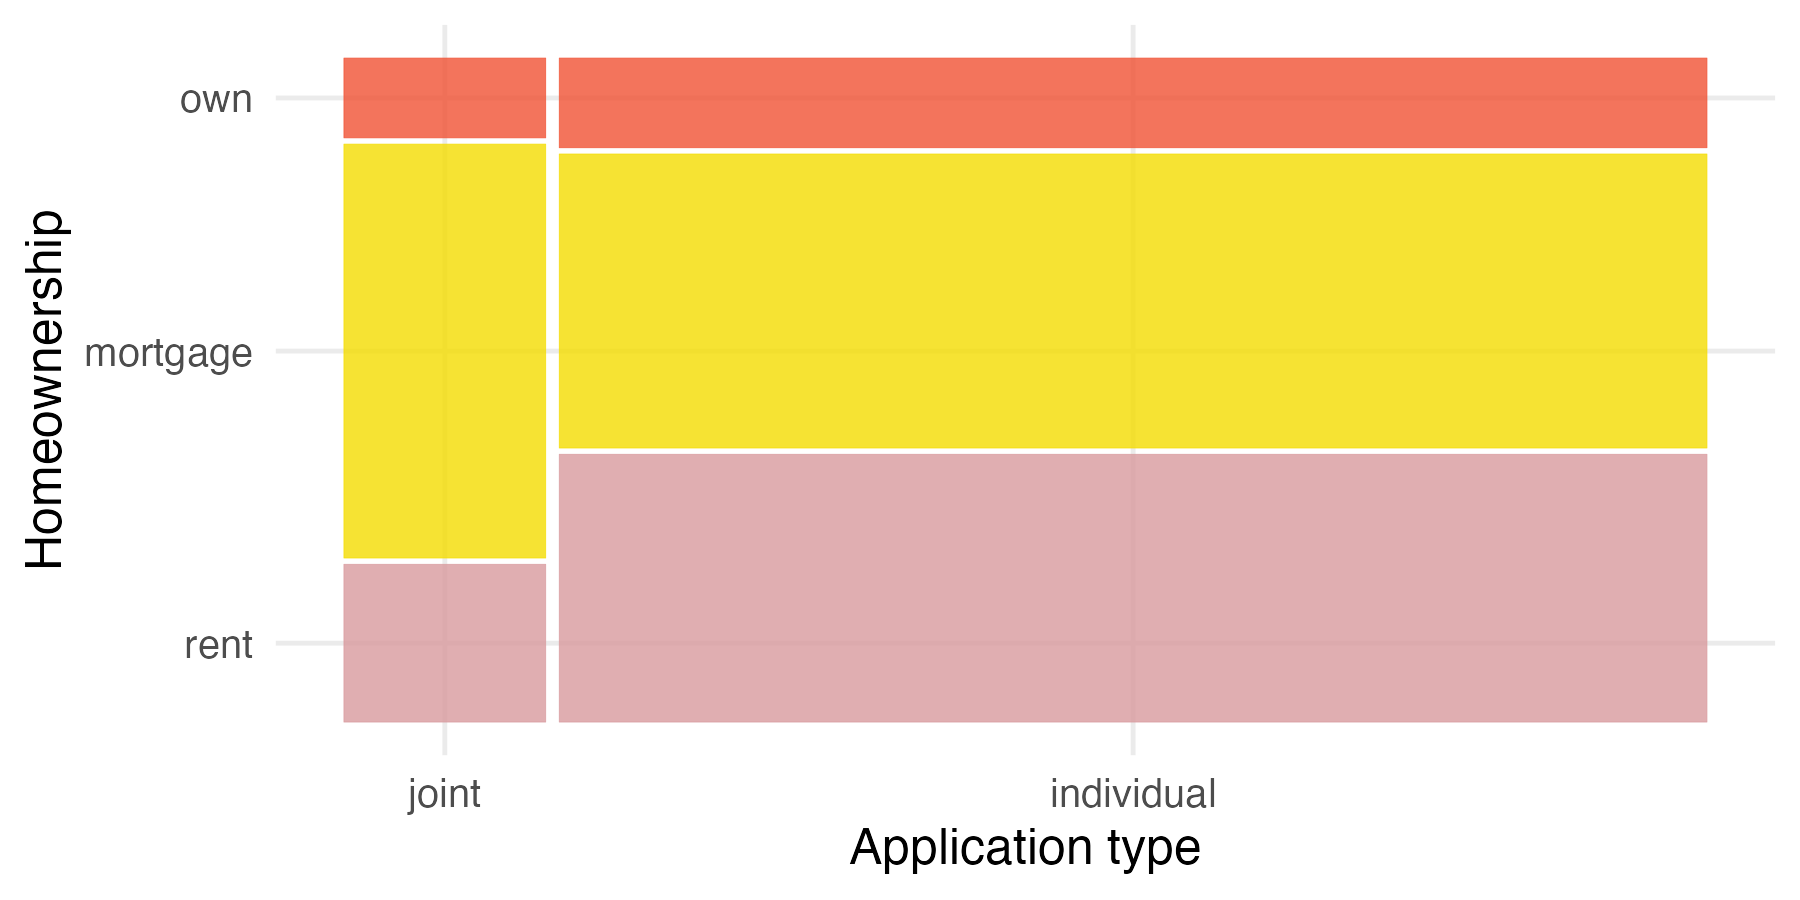
\includegraphics[width=0.8\textwidth,height=\textheight]{04-explore-categorical_files/figure-pdf/fig-loan-app-type-mosaic-plot-1.png}

}

\caption{\label{fig-loan-app-type-mosaic-plot}Mosaic plot where loans
are grouped by homeownership after they have been divided into
individual and joint application types.}

\end{figure}%

\vspace{-5mm}

\section{Row and column proportions}\label{row-and-column-proportions}

In the previous sections we inspected visualizations of two categorical
variables in bar plots and mosaic plots. However, we have not discussed
how the values in the bar and mosaic plots that show proportions are
calculated. In this section we will investigate fractional breakdown of
one variable in another and we can modify our contingency table to
provide such a view. Table~\ref{tbl-loan-home-app-type-row-proportions}
shows \textbf{row proportions} for
Table~\ref{tbl-loan-home-app-type-totals}, which are computed as the
counts divided by their row totals. The value 3496 at the intersection
of individual and rent is replaced by \(3496 / 8505 = 0.411,\) i.e.,
3496 divided by its row total, 8505. So, what does 0.411 represent? It
corresponds to the proportion of individual applicants who rent.

\begin{table}[H]

\caption{\label{tbl-loan-home-app-type-row-proportions}A contingency
table with row proportions for application type and homeownership.}

\centering{

\centering
\begin{tabular}[t]{>{\raggedright\arraybackslash}p{8em}>{\raggedleft\arraybackslash}p{5em}>{\raggedleft\arraybackslash}p{5em}>{\raggedleft\arraybackslash}p{5em}>{\raggedleft\arraybackslash}p{5em}}
\toprule
\multicolumn{1}{c}{ } & \multicolumn{3}{c}{homeownership} & \multicolumn{1}{c}{ } \\
\cmidrule(l{3pt}r{3pt}){2-4}
application\_type & rent & mortgage & own & Total\\
\midrule
\cellcolor{gray!10}{joint} & \cellcolor{gray!10}{0.242} & \cellcolor{gray!10}{0.635} & \cellcolor{gray!10}{0.122} & \cellcolor{gray!10}{1}\\
individual & 0.411 & 0.451 & 0.138 & 1\\
\bottomrule
\end{tabular}

}

\end{table}%

A contingency table of the \textbf{column proportions} is computed in a
similar way, where each is computed as the count divided by the
corresponding column total.
Table~\ref{tbl-loan-home-app-type-column-proportions} shows such a
table, and here the value 0.906 indicates that 90.6\% of renters applied
as individuals for the loan. This rate is higher compared to loans from
people with mortgages (80.2\%) or who own their home (86.5\%). Because
these rates vary between the three levels of \texttt{homeownership}
(\texttt{rent}, \texttt{mortgage}, \texttt{own}), this provides evidence
that \texttt{app\_type} and \texttt{homeownership} variables may be
associated.

\begin{table}[H]

\caption{\label{tbl-loan-home-app-type-column-proportions}A contingency
table with column proportions for application type and homeownership.}

\centering{

\centering
\begin{tabular}[t]{>{\raggedright\arraybackslash}p{8em}>{\raggedleft\arraybackslash}p{5em}>{\raggedleft\arraybackslash}p{5em}>{\raggedleft\arraybackslash}p{5em}>{}p{5em}}
\toprule
\multicolumn{1}{c}{ } & \multicolumn{3}{c}{homeownership} \\
\cmidrule(l{3pt}r{3pt}){2-4}
application\_type & rent & mortgage & own\\
\midrule
\cellcolor{gray!10}{joint} & \cellcolor{gray!10}{0.094} & \cellcolor{gray!10}{0.198} & \cellcolor{gray!10}{0.135}\\
individual & 0.906 & 0.802 & 0.865\\
\cellcolor{gray!10}{Total} & \cellcolor{gray!10}{1.000} & \cellcolor{gray!10}{1.000} & \cellcolor{gray!10}{1.000}\\
\bottomrule
\end{tabular}

}

\end{table}%

Row and column proportions can also be thought of as \textbf{conditional
proportions} as they tell us about the proportion of observations in a
given level of a categorical variable conditional on the level of
another categorical variable.

We could also have checked for an association between
\texttt{application\_type} and \texttt{homeownership} in
Table~\ref{tbl-loan-home-app-type-row-proportions} using row
proportions. When comparing these row proportions, we would look down
columns to see if the fraction of loans where the borrower rents, has a
mortgage, or owns varied across the application types.

\begin{guidedpractice}
What does 0.451 represent in
Table~\ref{tbl-loan-home-app-type-row-proportions}? What does 0.802
represent in
Table~\ref{tbl-loan-home-app-type-column-proportions}?\footnote{0.451
  represents the proportion of individual applicants who have a
  mortgage. 0.802 represents the fraction of applicants with mortgages
  who applied as individuals.}

\end{guidedpractice}

\vspace{-5mm}

\begin{guidedpractice}
What does 0.122 represent in
Table~\ref{tbl-loan-home-app-type-row-proportions}? What does 0.135
represent in
Table~\ref{tbl-loan-home-app-type-column-proportions}?\footnote{0.122
  represents the fraction of joint borrowers who own their home. 0.135
  represents the home-owning borrowers who had a joint application for
  the loan.}

\end{guidedpractice}

\vspace{-3mm}

\begin{workedexample}
Data scientists use statistics to build email spam filters. By noting
specific characteristics of an email, a data scientist may be able to
classify some emails as spam or not spam with high accuracy. One such
characteristic is the email format, which indicates whether an email has
any HTML content, such as bolded text. We'll focus on email format and
spam status using the dataset; these variables are summarized in a
contingency table in Table~\ref{tbl-email-count-table}. Which would be
more helpful to someone hoping to classify email as spam or regular
email for this table: row or column proportions?

\begin{center}\rule{0.5\linewidth}{0.5pt}\end{center}

A data scientist would be interested in how the proportion of spam
changes within each email format. This corresponds to column
proportions: the proportion of spam in plain text emails and the
proportion of spam in HTML emails. If we generate the column
proportions, we can see that a higher fraction of plain text emails are
spam (\(209/1195 = 17.5\%\)) than compared to HTML emails
(\(158/2726 = 5.8\%\)). This information on its own is insufficient to
classify an email as spam or not spam, as over 80\% of plain text emails
are not spam. Yet, when we carefully combine this information with many
other characteristics, we stand a reasonable chance of being able to
classify some emails as spam or not spam with confidence. This example
points out that row and column proportions are not equivalent. Before
settling on one form for a table, it is important to consider each to
ensure that the most useful table is constructed. However, sometimes it
simply isn't clear which, if either, is more useful.

\end{workedexample}

\vspace{-5mm}

\begin{data}
The
\href{http://openintrostat.github.io/openintro/reference/email.html}{email}
data can be found in the
\href{http://openintrostat.github.io/openintro}{\textbf{openintro}} R
package.

\end{data}

\vspace{-4mm}

\begin{table}[H]

\caption{\label{tbl-email-count-table}A contingency table for spam and
format.}

\centering{

\centering
\begin{tabular}[t]{>{\raggedright\arraybackslash}p{8em}>{\raggedleft\arraybackslash}p{5em}>{\raggedleft\arraybackslash}p{5em}>{\raggedleft\arraybackslash}p{5em}>{}p{5em}}
\toprule
spam & HTML & text & Total\\
\midrule
\cellcolor{gray!10}{not spam} & \cellcolor{gray!10}{2568} & \cellcolor{gray!10}{986} & \cellcolor{gray!10}{3554}\\
spam & 158 & 209 & 367\\
\cellcolor{gray!10}{Total} & \cellcolor{gray!10}{2726} & \cellcolor{gray!10}{1195} & \cellcolor{gray!10}{3921}\\
\bottomrule
\end{tabular}

}

\end{table}%

\clearpage

\begin{workedexample}
Look back to Table~\ref{tbl-loan-home-app-type-row-proportions} and
Table~\ref{tbl-loan-home-app-type-column-proportions}. Are there any
obvious scenarios where one might be more useful than the other?

\begin{center}\rule{0.5\linewidth}{0.5pt}\end{center}

None that we think are obvious! What is distinct about the email example
is that the two loan variables do not have a clear explanatory-response
variable relationship that we might hypothesize. Usually it is most
useful to ``condition'' on the explanatory variable. For instance, in
the email example, the email format was seen as a possible explanatory
variable of whether the message was spam, so we would find it more
interesting to compute the relative frequencies (proportions) for each
email format.

\end{workedexample}

\section{Pie charts}\label{pie-charts}

A \textbf{pie chart} is shown in
Figure~\ref{fig-loan-homeownership-pie-chart-1} alongside a bar plot
representing the same information in
Figure~\ref{fig-loan-homeownership-pie-chart-2}. Pie charts can be
useful for giving a high-level overview to show how a set of cases break
down. However, it is also difficult to decipher certain details in a pie
chart. For example, it's not immediately obvious that there are more
loans where the borrower has a mortgage than rent when looking at the
pie chart, while this detail is very obvious in the bar plot.

\begin{figure}[H]

\begin{minipage}{0.47\linewidth}

\centering{

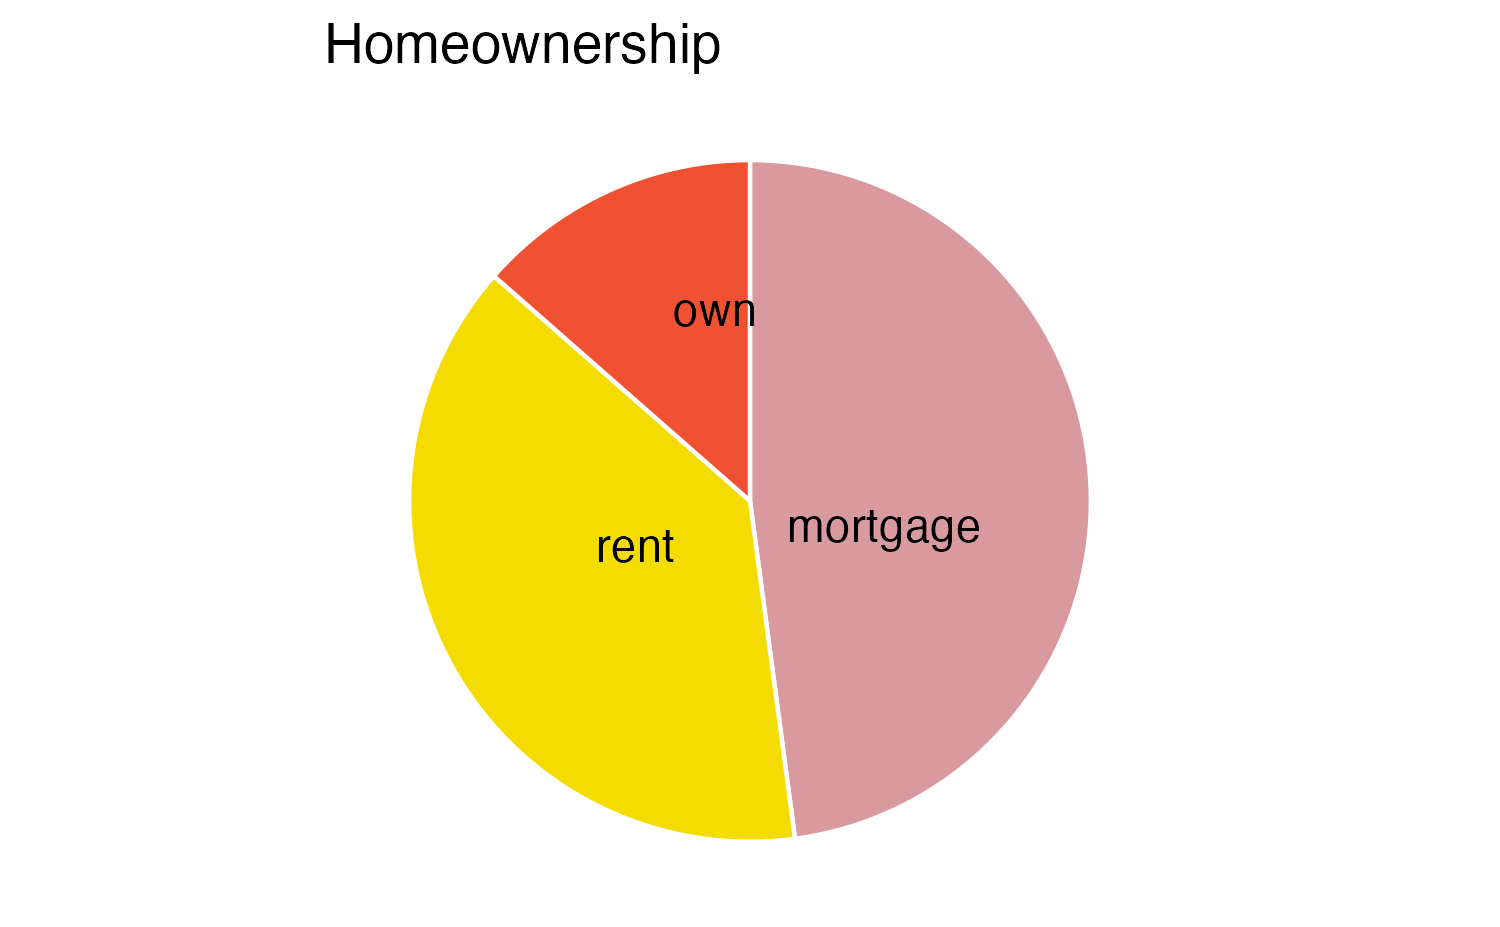
\includegraphics[width=1\textwidth,height=\textheight]{04-explore-categorical_files/figure-pdf/fig-loan-homeownership-pie-chart-1.png}

}

\subcaption{\label{fig-loan-homeownership-pie-chart-1}Pie chart}

\end{minipage}%
%
\begin{minipage}{0.06\linewidth}
~\end{minipage}%
%
\begin{minipage}{0.47\linewidth}

\centering{

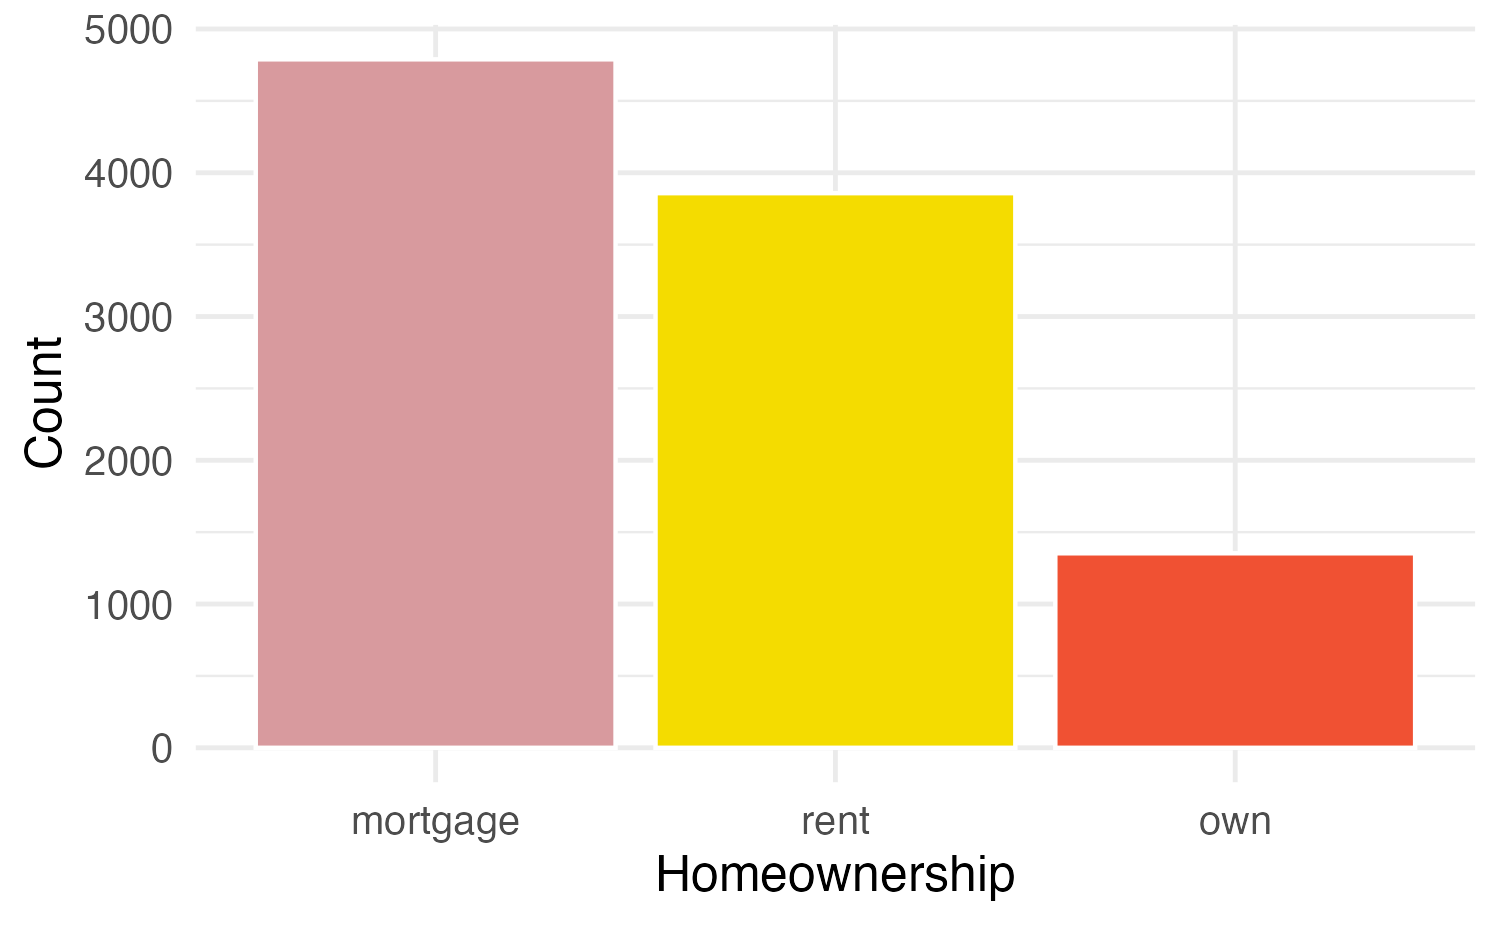
\includegraphics[width=1\textwidth,height=\textheight]{04-explore-categorical_files/figure-pdf/fig-loan-homeownership-pie-chart-2.png}

}

\subcaption{\label{fig-loan-homeownership-pie-chart-2}Bar plot}

\end{minipage}%

\caption{\label{fig-loan-homeownership-pie-chart}A pie chart and bar
plot of homeownership.}

\end{figure}%

Pie charts can work well when the goal is to visualize a categorical
variable with very few levels, and especially if each level represents a
simple fraction (e.g., one-half, one-quarter, etc.). However, they can
be quite difficult to read when they are used to visualize a categorical
variable with many levels. For example, the pie chart
Figure~\ref{fig-loan-grade-pie-chart-1} and the
Figure~\ref{fig-loan-grade-pie-chart-2} both represent the distribution
of loan grades (A through G). In this case, it is far easier to compare
the counts of each loan grade using the bar plot than the pie chart.

\begin{figure}[H]

\begin{minipage}{0.47\linewidth}

\centering{

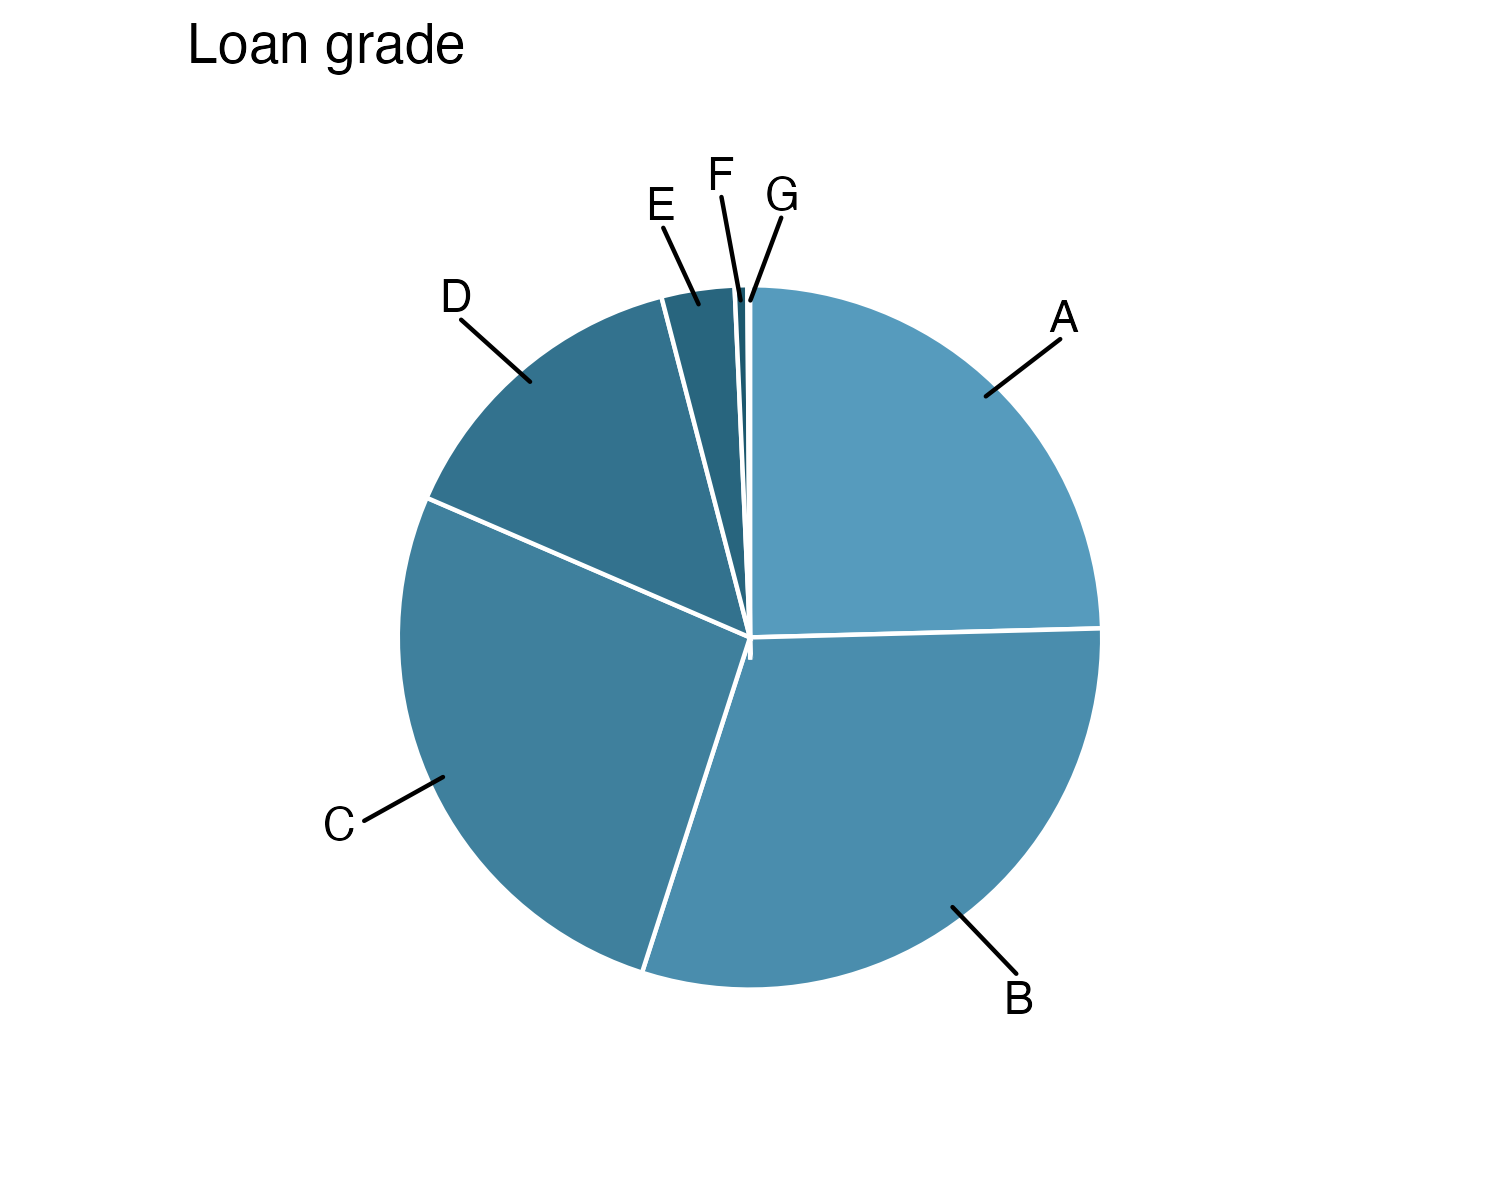
\includegraphics[width=1\textwidth,height=\textheight]{04-explore-categorical_files/figure-pdf/fig-loan-grade-pie-chart-1.png}

}

\subcaption{\label{fig-loan-grade-pie-chart-1}Pie chart}

\end{minipage}%
%
\begin{minipage}{0.06\linewidth}
~\end{minipage}%
%
\begin{minipage}{0.47\linewidth}

\centering{

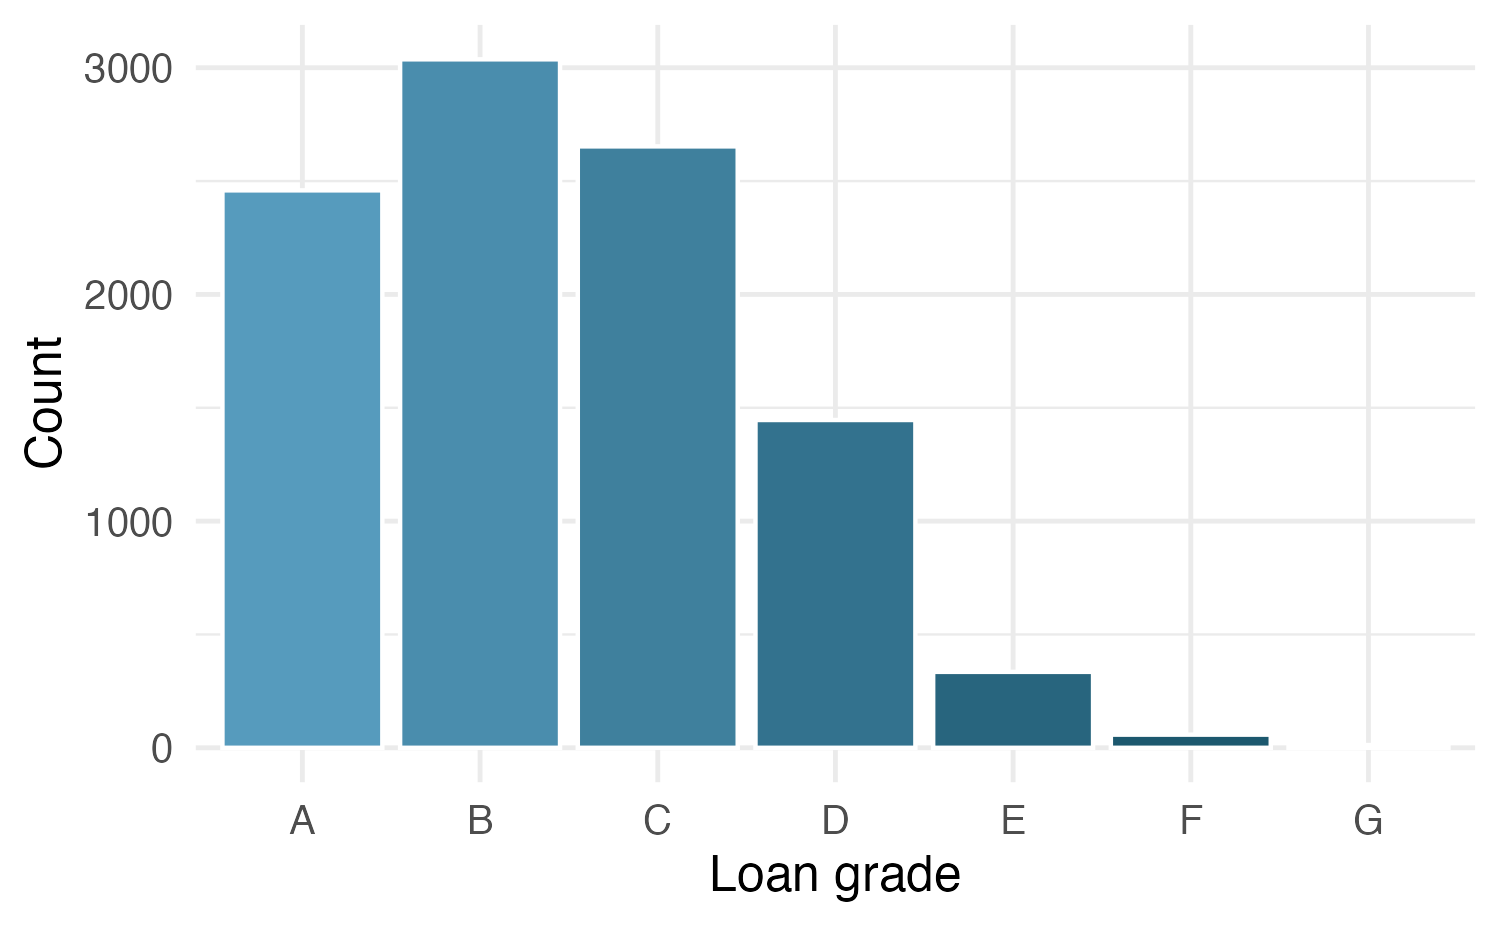
\includegraphics[width=1\textwidth,height=\textheight]{04-explore-categorical_files/figure-pdf/fig-loan-grade-pie-chart-2.png}

}

\subcaption{\label{fig-loan-grade-pie-chart-2}Bar plot}

\end{minipage}%

\caption{\label{fig-loan-grade-pie-chart}A pie chart and bar plot of
loan grades.}

\end{figure}%

\section{Waffle charts}\label{waffle-charts}

Another useful technique of visualizing categorical data is a
\textbf{waffle chart}. Waffle charts can be used to communicate the
proportion of the data that falls into each level of a categorical
variable. Just like with pie charts, they work best when the number of
levels represented is low. However, unlike pie charts, they can make it
easier to compare proportions that represent non-simple fractions.
Figure~\ref{fig-loan-waffle-1} and Figure~\ref{fig-loan-waffle-2}
display two examples of waffle charts: one of homeownership and one of
loan status, respectively.

\begin{figure}[H]

\begin{minipage}{0.47\linewidth}

\centering{

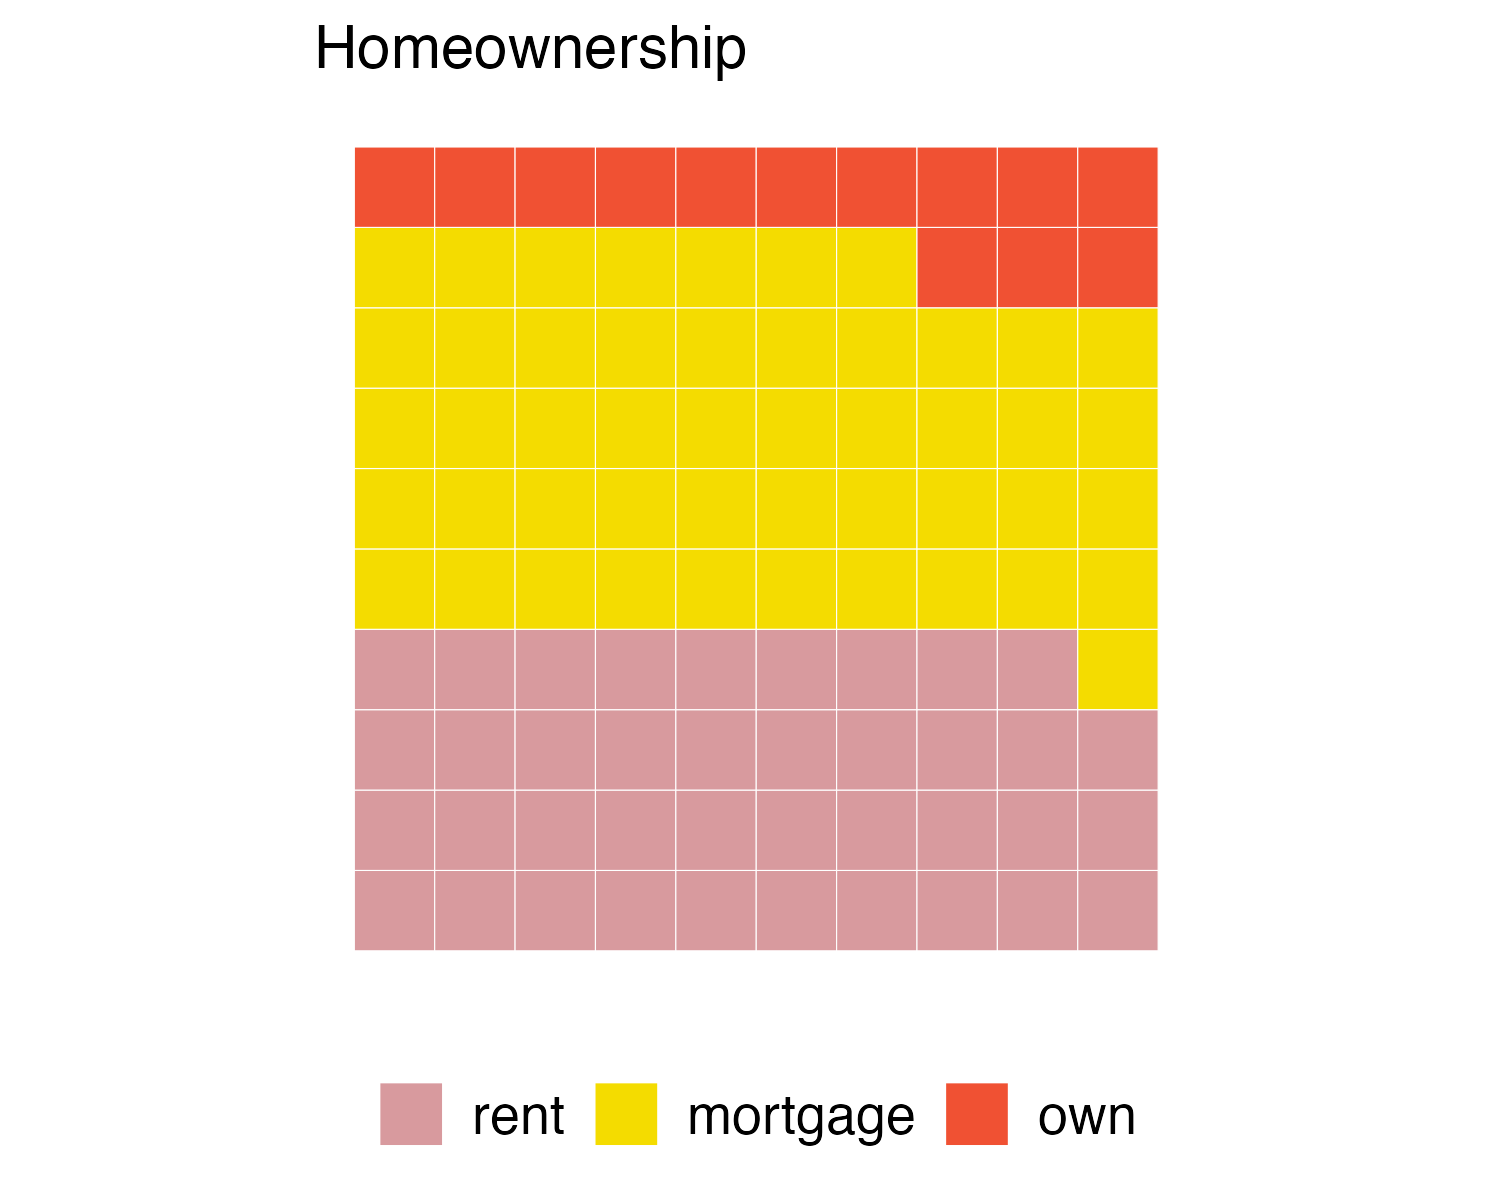
\includegraphics[width=1\textwidth,height=\textheight]{04-explore-categorical_files/figure-pdf/fig-loan-waffle-1.png}

}

\subcaption{\label{fig-loan-waffle-1}Homeownership, with levels rent,
mortgage, and own.}

\end{minipage}%
%
\begin{minipage}{0.06\linewidth}
~\end{minipage}%
%
\begin{minipage}{0.47\linewidth}

\centering{

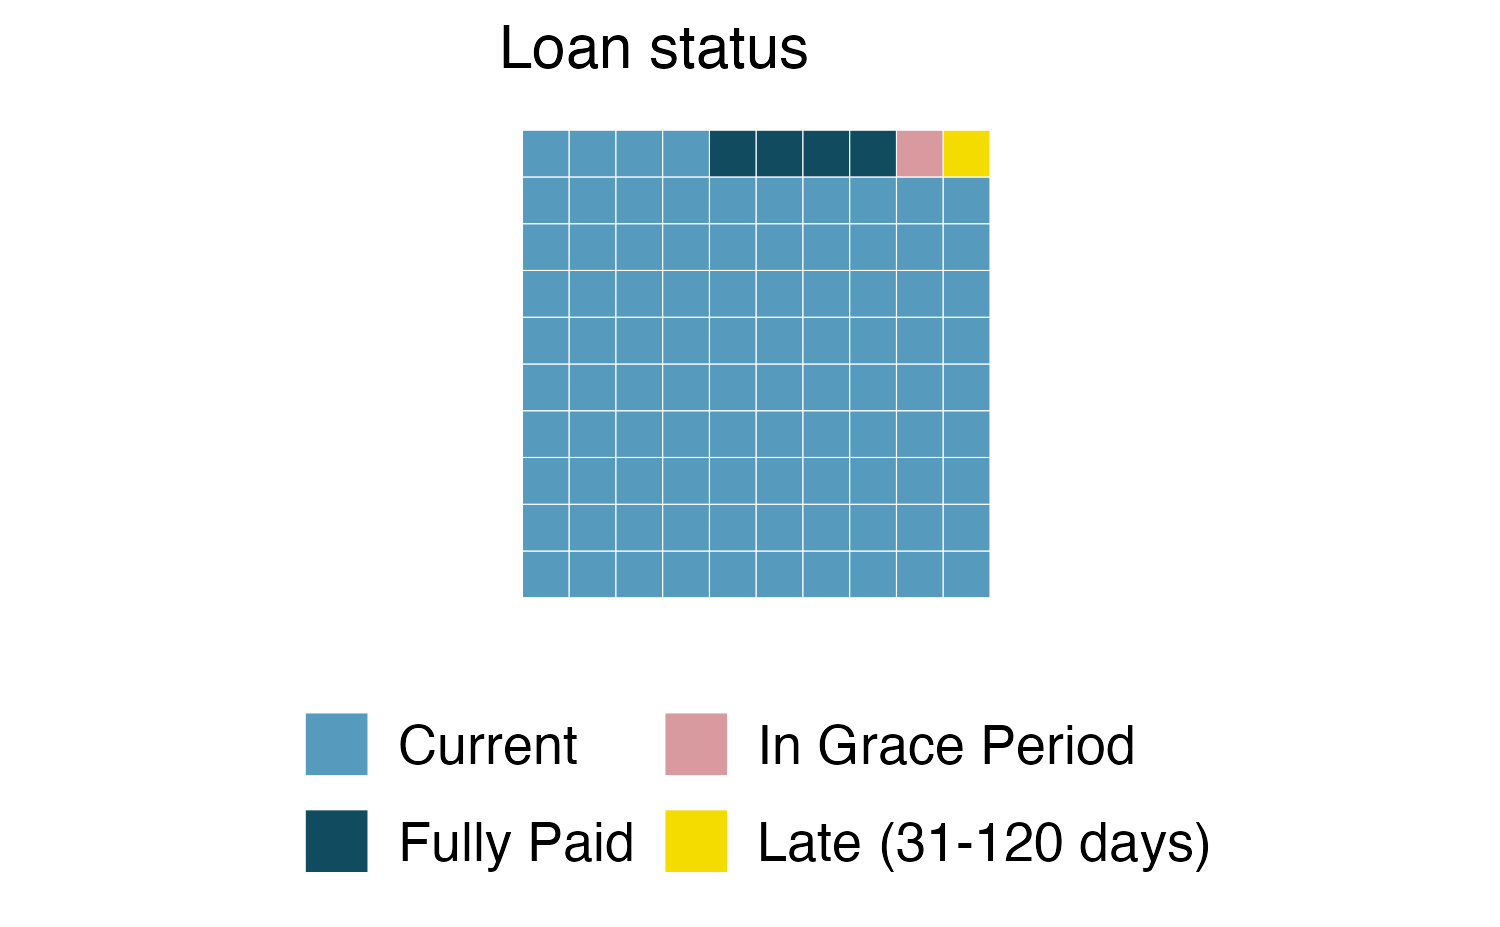
\includegraphics[width=1\textwidth,height=\textheight]{04-explore-categorical_files/figure-pdf/fig-loan-waffle-2.png}

}

\subcaption{\label{fig-loan-waffle-2}Loan status, with levels current,
fully paid, in grace period, and late.}

\end{minipage}%

\caption{\label{fig-loan-waffle}Waffle charts of homeownership and loan
status.}

\end{figure}%

\section{Comparing numerical data across
groups}\label{comparing-numerical-data-across-groups}

Some of the more interesting investigations can be considered by
examining numerical data across groups. In this section we will expand
on a few methods we have already seen to make plots for numerical data
from multiple groups on the same graph as well as introduce a few new
methods for comparing numerical data across groups.

We will revisit the \texttt{county} dataset and compare the median
household income for counties that gained population from 2010 to 2017
versus counties that had no gain. While we might like to make a causal
connection between income and population growth, remember that these are
observational data and so such an interpretation would be, at best,
half-baked.

We have data on 3142 counties in the United States. We are missing 2017
population data from 3 of them, and of the remaining 3139 counties, in
1541 the population increased from 2010 to 2017 and in the remaining
1598 the population decreased.
Table~\ref{tbl-countyIncomeSplitByPopGainTable} shows a sample of 5
observations from each group.

\begin{table}[H]

\caption{\label{tbl-countyIncomeSplitByPopGainTable}The median household
income from a random sample of 5 counties with population gain between
2010 to 2017 and another random sample of 5 counties with no population
gain.}

\centering{

\centering
\begin{tabular}[t]{ll>{\centering\arraybackslash}p{8em}>{\centering\arraybackslash}p{4em}>{\centering\arraybackslash}p{8em}}
\toprule
State & County & Population change (\%) & Gain / No gain & Median household income\\
\midrule
\cellcolor{gray!10}{Arkansas} & \cellcolor{gray!10}{Izard County} & \cellcolor{gray!10}{2.13} & \cellcolor{gray!10}{gain} & \cellcolor{gray!10}{39135}\\
Georgia & Jackson County & 10.17 & gain & 57999\\
\cellcolor{gray!10}{Oregon} & \cellcolor{gray!10}{Hood River County} & \cellcolor{gray!10}{3.41} & \cellcolor{gray!10}{gain} & \cellcolor{gray!10}{57269}\\
Texas & Montague County & 0.75 & gain & 46592\\
\cellcolor{gray!10}{Virginia} & \cellcolor{gray!10}{Appomattox County} & \cellcolor{gray!10}{2.38} & \cellcolor{gray!10}{gain} & \cellcolor{gray!10}{54875}\\
Kentucky & Ballard County & -2.62 & no gain & 42988\\
\cellcolor{gray!10}{Kentucky} & \cellcolor{gray!10}{Fleming County} & \cellcolor{gray!10}{-0.71} & \cellcolor{gray!10}{no gain} & \cellcolor{gray!10}{41095}\\
Kentucky & Letcher County & -5.13 & no gain & 30293\\
\cellcolor{gray!10}{Maine} & \cellcolor{gray!10}{Penobscot County} & \cellcolor{gray!10}{-0.73} & \cellcolor{gray!10}{no gain} & \cellcolor{gray!10}{47886}\\
Virginia & Richmond County & -0.19 & no gain & 47341\\
\bottomrule
\end{tabular}

}

\end{table}%

Color can be used to split histograms (see Section~\ref{sec-histograms}
for an introduction to histograms) for numerical variables by levels of
a categorical variable. An example of this is shown in
Figure~\ref{fig-countyIncomeSplitByPopGain-1}. The \textbf{side-by-side
box plot} is another traditional tool for comparing across groups. An
example is shown in Figure~\ref{fig-countyIncomeSplitByPopGain-2}, where
there are two box plots (see Section~\ref{sec-boxplots} for an
introduction to box plots), one for each group, placed into one plotting
window and drawn on the same scale.

\begin{figure}[H]

\centering{

\centering{

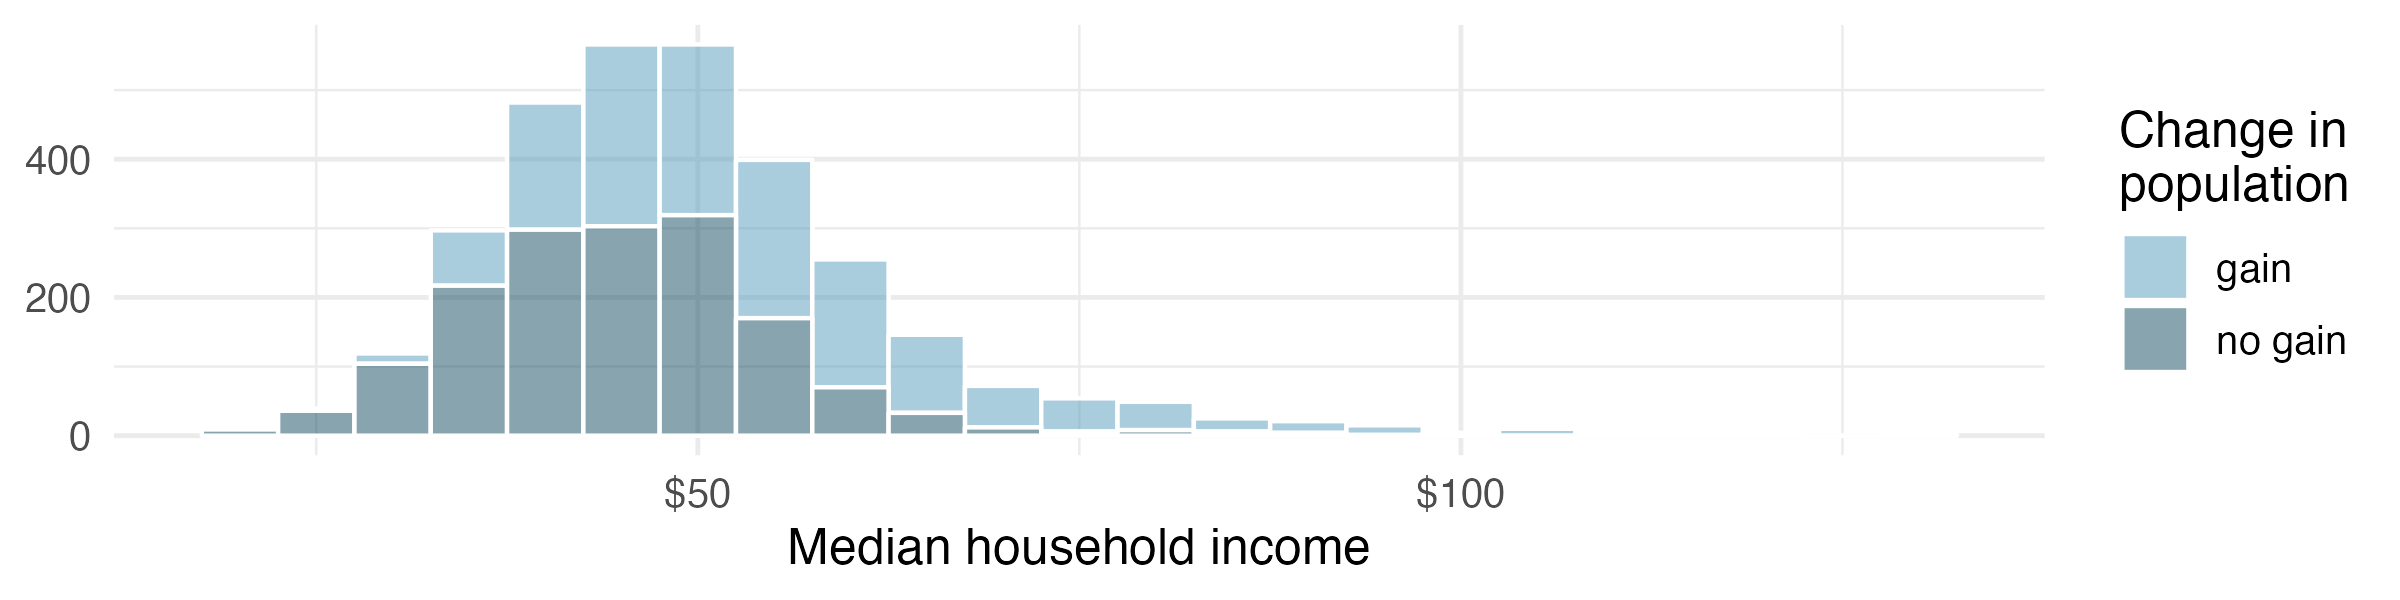
\includegraphics[width=0.9\textwidth,height=\textheight]{04-explore-categorical_files/figure-pdf/fig-countyIncomeSplitByPopGain-1.png}

}

\subcaption{\label{fig-countyIncomeSplitByPopGain-1}Histograms}

\centering{

\includegraphics[width=0.9\textwidth,height=\textheight]{04-explore-categorical_files/figure-pdf/fig-countyIncomeSplitByPopGain-2.png}

}

\subcaption{\label{fig-countyIncomeSplitByPopGain-2}Side by-side box
plots}

}

\caption{\label{fig-countyIncomeSplitByPopGain}Visualizations of median
household income of counties by change in population (gain or loss).}

\end{figure}%

\begin{guidedpractice}
Use the plots in Figure~\ref{fig-countyIncomeSplitByPopGain} to compare
the incomes for counties across the two groups. What do you notice about
the approximate center of each group? What do you notice about the
variability between groups? Is the shape relatively consistent between
groups? How many \emph{prominent} modes are there for each
group?\footnote{Answers may vary a little. The counties with population
  gains tend to have higher income (median of about \$45,000) versus
  counties without a gain (median of about \$40,000). The variability is
  also slightly larger for the population gain group. This is evident in
  the IQR, which is about 50\% bigger in the \emph{gain} group. Both
  distributions show slight to moderate right skew and are unimodal. The
  box plots indicate there are many observations far above the median in
  each group, though we should anticipate that many observations will
  fall beyond the whiskers when examining any dataset that contain more
  than a few hundred data points.}

\end{guidedpractice}

\begin{guidedpractice}
What components of each plot in
Figure~\ref{fig-countyIncomeSplitByPopGain} do you find most
useful?\footnote{Answers will vary. The side-by-side box plots are
  especially useful for comparing centers and spreads, while the hollow
  histograms are more useful for seeing distribution shape, skew, modes,
  and potential anomalies.}

\end{guidedpractice}

Another useful visualization for comparing numerical data across groups
is a \textbf{ridge plot}, which combines density plots (see
Section~\ref{sec-boxplots} for an introduction to density plots) for
various groups drawn on the same scale in a single plotting window.
Figure~\ref{fig-countyIncomeSplitByPopGainRidge} displays a ridge plot
for the distribution of median household income in counties, split by
whether there was a population gain or not.

\begin{figure}[H]

\centering{

\includegraphics[width=0.9\textwidth,height=\textheight]{04-explore-categorical_files/figure-pdf/fig-countyIncomeSplitByPopGainRidge-1.png}

}

\caption{\label{fig-countyIncomeSplitByPopGainRidge}Ridge plot for
median household income, where counties are split by whether there was a
population gain or not.}

\end{figure}%

\begin{guidedpractice}
What components of the ridge plot in
Figure~\ref{fig-countyIncomeSplitByPopGainRidge} do you find most useful
compared to those in
Figure~\ref{fig-countyIncomeSplitByPopGain}?\footnote{The ridge plot
  give us a better sense of the shape, and especially modality, of the
  data.}

\end{guidedpractice}

One last visualization technique we'll highlight for comparing numerical
data across groups is \textbf{faceting}. In this technique we split
(facet) the graphical display of the data across plotting windows based
on groups. Plot A in
Figure~\ref{fig-countyIncomeSplitByPopGainFacetHist} displays the same
information as Figure~\ref{fig-countyIncomeSplitByPopGain-1}, however
here the distributions of median household income for counties with and
without population gain are faceted across two plotting windows. We
preserve the same scale on the x and y axes for easier comparison. An
advantage of this approach is that it extends to splitting the data
across levels of two categorical variables, which allows for displaying
relationships between three variables. In Plot B in
Figure~\ref{fig-countyIncomeSplitByPopGainFacetHist} we have now split
the data into four groups using the \texttt{pop\_change} and
\texttt{metro} variables:

\begin{itemize}
\tightlist
\item
  top left represents counties that are \emph{not} in a
  \texttt{metro}politan area with population gain,
\item
  top right represents counties that are in a metropolitan area with
  population gain,
\item
  bottom left represents counties that are \emph{not} in a metropolitan
  area without population gain, and finally
\item
  bottom right represents counties that are in a metropolitan area
  without population gain.
\end{itemize}

\begin{figure}[H]

\begin{minipage}{0.30\linewidth}

\centering{

\includegraphics[width=1\textwidth,height=\textheight]{04-explore-categorical_files/figure-pdf/fig-countyIncomeSplitByPopGainFacetHist-1-1.png}

}

\subcaption{\label{fig-countyIncomeSplitByPopGainFacetHist-1}By
population gain.}

\end{minipage}%
%
\begin{minipage}{0.70\linewidth}

\centering{

\includegraphics[width=1\textwidth,height=\textheight]{04-explore-categorical_files/figure-pdf/fig-countyIncomeSplitByPopGainFacetHist-2-1.png}

}

\subcaption{\label{fig-countyIncomeSplitByPopGainFacetHist-2}By both
population gain and metropolitan area.}

\end{minipage}%

\caption{\label{fig-countyIncomeSplitByPopGainFacetHist}Distribution of
median income in counties using faceted histograms.}

\end{figure}%

We can continue building upon this visualization to add one more
variable, \texttt{median\_edu}, which is the median education level in
the county. In Figure~\ref{fig-countyIncomeRidgeMulti}, we represent
median education level using color, where pink (solid line) represents
counties where the median education level is high school diploma, yellow
(dashed line) is some college degree, and red (dotted line) is
Bachelor's.

\begin{guidedpractice}
Based on Figure~\ref{fig-countyIncomeRidgeMulti}, what can you say about
how median household income in counties vary depending on population
gain/no gain, metropolitan area/not, and median degree?\footnote{Regardless
  of the location (metropolitan or not) or change in population, it
  seems like there is an increase in median household income from
  individuals with only a HS diploma, to individuals with some college,
  to individuals with a Bachelor's degree.}

\end{guidedpractice}

\begin{figure}[H]

\centering{

\includegraphics[width=1\textwidth,height=\textheight]{04-explore-categorical_files/figure-pdf/fig-countyIncomeRidgeMulti-1.png}

}

\caption{\label{fig-countyIncomeRidgeMulti}Distribution of median income
in counties using a ridge plot, faceted by whether the county had a
population gain or not as well as whether the county is in a
metropolitan area and colored by the median education level in the
county.}

\end{figure}%

\vfill

\section{Chapter review}\label{sec-chp4-review}

\subsection{Summary}\label{summary-2}

Fluently working with categorical variables is an important skill for
data analysts. In this chapter we have introduced different
visualizations and numerical summaries applied to categorical variables.
The graphical visualizations are even more descriptive when two
variables are presented simultaneously. We presented bar plots, mosaic
plots, pie charts, and estimations of conditional proportions.

\subsection{Terms}\label{terms-2}

The terms introduced in this chapter are presented in
Table~\ref{tbl-terms-chp-04}. If you're not sure what some of these
terms mean, we recommend you go back in the text and review their
definitions. You should be able to easily spot them as \textbf{bolded
text}.

\begin{table}[H]

\caption{\label{tbl-terms-chp-04}Terms introduced in this chapter.}

\centering{

\centering
\begin{tabular}[t]{>{\raggedright\arraybackslash}p{12em}>{\raggedright\arraybackslash}p{12em}>{\raggedright\arraybackslash}p{12em}}
\toprule
\cellcolor{gray!10}{column proportions} & \cellcolor{gray!10}{faceted plot} & \cellcolor{gray!10}{row totals}\\
column totals & filled bar plot & side-by-side box plot\\
\cellcolor{gray!10}{conditional proportions} & \cellcolor{gray!10}{mosaic plot} & \cellcolor{gray!10}{stacked bar plot}\\
contingency table & ridge plot & standardized bar plot\\
\cellcolor{gray!10}{dodged bar plot} & \cellcolor{gray!10}{row proportions} & \cellcolor{gray!10}{}\\
\bottomrule
\end{tabular}

}

\end{table}%

\vfill

\clearpage

\section{Exercises}\label{sec-chp4-exercises}

Answers to odd-numbered exercises can be found in
Appendix~\ref{sec-exercise-solutions-04}.

\begin{exercises}

\begin{enumerate}
\def\labelenumi{\arabic{enumi}.}
\item
  \textbf{Antibiotic use in children.} The bar plot and the pie chart
  below show the distribution of pre-existing medical conditions of
  children involved in a study on the optimal duration of antibiotic use
  in treatment of tracheitis, which is an upper respiratory
  infection.\footnote{The
    \href{http://openintrostat.github.io/openintro/reference/antibiotics.html}{\texttt{antibiotics}}
    data used in this exercise can be found in the
    \href{http://openintrostat.github.io/openintro}{\textbf{openintro}}
    R package.}

  \includegraphics[width=0.95\textwidth,height=\textheight]{04-explore-categorical_files/figure-pdf/unnamed-chunk-30-1.png}

  \begin{enumerate}
  \def\labelenumii{\alph{enumii}.}
  \item
    What features are apparent in the bar plot but not in the pie chart?
  \item
    What features are apparent in the pie chart but not in the bar plot?
  \item
    Which graph would you prefer to use for displaying these categorical
    data?
  \end{enumerate}
\end{enumerate}

\vspace{10mm}

\begin{enumerate}
\def\labelenumi{\arabic{enumi}.}
\setcounter{enumi}{1}
\item
  \textbf{Views on immigration.} Nine-hundred and ten (910) randomly
  sampled registered voters from Tampa, FL were asked if they thought
  workers who have illegally entered the US should be (i) allowed to
  keep their jobs and apply for US citizenship, (ii) allowed to keep
  their jobs as temporary guest workers but not allowed to apply for US
  citizenship, or (iii) lose their jobs and have to leave the country.
  The results of the survey by political ideology are shown
  below.\footnote{The
    \href{http://openintrostat.github.io/openintro/reference/immigration.html}{\texttt{immigration}}
    data used in this exercise can be found in the
    \href{http://openintrostat.github.io/openintro}{\textbf{openintro}}
    R package.}

  \begin{table}[H]
  \centering
  \begin{tabular}[t]{lrrrr}
  \toprule
  Response & Conservative & Liberal & Moderate & Total\\
  \midrule
  Apply for citizenship & 57 & 101 & 120 & 278\\
  Guest worker & 121 & 28 & 113 & 262\\
  Leave the country & 179 & 45 & 126 & 350\\
  Not sure & 15 & 1 & 4 & 20\\
  Total & 372 & 175 & 363 & 910\\
  \bottomrule
  \end{tabular}
  \end{table}

  \clearpage

  \begin{enumerate}
  \def\labelenumii{\alph{enumii}.}
  \item
    What percent of these Tampa, FL voters identify themselves as
    conservatives?
  \item
    What percent of these Tampa, FL voters are in favor of the
    citizenship option?
  \item
    What percent of these Tampa, FL voters identify themselves as
    conservatives and are in favor of the citizenship option?
  \item
    What percent of these Tampa, FL voters who identify themselves as
    conservatives are also in favor of the citizenship option? What
    percent of moderates share this view? What percent of liberals share
    this view?
  \item
    Do political ideology and views on immigration appear to be
    associated? Explain your reasoning.
  \item
    Conjecture other possible variables that might explain the potential
    relationship between these two variables.
  \end{enumerate}
\end{enumerate}

\vfill

\begin{enumerate}
\def\labelenumi{\arabic{enumi}.}
\setcounter{enumi}{2}
\item
  \textbf{Black Lives Matter.} A Washington Post-Schar School poll
  conducted in the United States in June 2020, among a random national
  sample of 1,006 adults, asked respondents whether they support or
  oppose protests following George Floyd's killing that have taken place
  in cities across the US. The survey also collected information on the
  age of the respondents. (Washington Post 2020) The results are
  summarized in the stacked bar plot below.

  \includegraphics[width=0.95\textwidth,height=\textheight]{04-explore-categorical_files/figure-pdf/unnamed-chunk-32-1.png}

  \begin{enumerate}
  \def\labelenumii{\alph{enumii}.}
  \item
    Based on the stacked bar plot, do views on the protests and age
    appear to be associated? Explain your reasoning.
  \item
    Conjecture other possible variables that might explain the potential
    association between these two variables.
  \end{enumerate}
\end{enumerate}

\vfill

\clearpage

\begin{enumerate}
\def\labelenumi{\arabic{enumi}.}
\setcounter{enumi}{3}
\item
  \textbf{Raise taxes.} A random sample of registered voters nationally
  were asked whether they think it's better to raise taxes on the rich
  or raise taxes on the poor. The survey also collected information on
  the political party affiliation of the respondents. (Polling 2015)

  \includegraphics[width=0.95\textwidth,height=\textheight]{04-explore-categorical_files/figure-pdf/unnamed-chunk-33-1.png}

  \begin{enumerate}
  \def\labelenumii{\alph{enumii}.}
  \item
    Based on the stacked bar plot shown above, do views on raising taxes
    and political affiliation appear to be associated? Explain your
    reasoning.
  \item
    Conjecture other possible variables that might explain the potential
    association between these two variables.
  \end{enumerate}
\end{enumerate}

\vfill

\begin{enumerate}
\def\labelenumi{\arabic{enumi}.}
\setcounter{enumi}{4}
\item
  \textbf{Heart transplant data display.} The Stanford University Heart
  Transplant Study was conducted to determine whether an experimental
  heart transplant program increased lifespan. Each patient entering the
  program was officially designated a heart transplant candidate,
  meaning that they were gravely ill and might benefit from a new heart.
  Patients were randomly assigned into treatment and control groups.
  Patients in the treatment group received a transplant, and those in
  the control group did not. The visualizations below display two
  different versions of the study results.\footnote{The
    \href{http://openintrostat.github.io/openintro/reference/heart_transplant.html}{\texttt{heart\_transplant}}
    data used in this exercise can be found in the
    \href{http://openintrostat.github.io/openintro}{\textbf{openintro}}
    R package.} (Turnbull, Brown, and Hu 1974)

  \includegraphics[width=0.95\textwidth,height=\textheight]{04-explore-categorical_files/figure-pdf/unnamed-chunk-34-1.png}

  \begin{enumerate}
  \def\labelenumii{\alph{enumii}.}
  \item
    Provide one aspect of the two group comparison that is easier to see
    from the stacked bar plot (left)?
  \item
    Provide one aspect of the two group comparison that is easeir to see
    from the standardized bar plot (right)?
  \item
    For the Heart Transplant Study which of those aspects would be more
    important to display? That is, which bar plot would be better as a
    data visualization?
  \end{enumerate}
\end{enumerate}

\vfill

\clearpage

\begin{enumerate}
\def\labelenumi{\arabic{enumi}.}
\setcounter{enumi}{5}
\item
  \textbf{Shipping holiday gifts data display.} A local news survey
  asked 500 randomly sampled Los Angeles residents which shipping
  carrier they prefer to use for shipping holiday gifts. The bar plots
  below show the distribution of responses by age group as well as
  distribution of responses by shipping method.

  \includegraphics[width=0.95\textwidth,height=\textheight]{04-explore-categorical_files/figure-pdf/unnamed-chunk-35-1.png}

  \begin{enumerate}
  \def\labelenumii{\alph{enumii}.}
  \item
    Which graph (top or bottom) would you use to understand the shipping
    choices of people of different ages? Explain.
  \item
    Which graph (top or bottom) would you use to understand the age
    distribution across different types of shipping choices? Explain.
  \item
    A new shipping company would like to market to people over the age
    of 55. Who will be their biggest competitor? Explain.
  \item
    FedEx would like to reach out to grow their market share so as to
    balance the age demographics of FedEx users. To what age group
    should FedEx market?
  \end{enumerate}
\end{enumerate}

\clearpage

\begin{enumerate}
\def\labelenumi{\arabic{enumi}.}
\setcounter{enumi}{6}
\item
  \textbf{Meat consumption and life expectancy.} In data collected for
  You et al. (2022), total meat intake is associated with life
  expectancy (at birth) in 175 countries. Meat intake is measured in kg
  per capita per year (averaged over 2011 to 2013). The two ridge plots
  show an association between income and meat consumption (higher income
  countries tend to eat more meat) and an association between income and
  life expectancy (higher income countries have higher life expectancy).

  \includegraphics[width=0.95\textwidth,height=\textheight]{04-explore-categorical_files/figure-pdf/unnamed-chunk-36-1.png}

  \begin{enumerate}
  \def\labelenumii{\alph{enumii}.}
  \item
    Do the graphs above demonstrate that meat consumption and life
    expectancy are associated? That is, can you tell if countries with
    low meat consumption have low life expectancy? Explain.
  \item
    Let's assume that you had a plot comparing meat consumption and life
    expectancy, and they \emph{do} seem associated. Your friend says
    that the plot shows that high meat consumption leads to a longer
    life. You correctly say, no, we can't tell if there is a causal
    realtionship because the relationship is confounded by income level.
    Explain what you mean.
  \item
    How can you investigate the relationship between meat consumption
    and life expectancy in the presence of confounding variables (like
    income)?
  \end{enumerate}
\item
  \textbf{Florence Nightingale.} Florence Nightingale was a nurse in the
  Crimean War and an early statistician. In her notes, she opined, ``In
  comparing the deaths of one hospital with those of another, any
  statistics are justly considered absolutely valueless which do not
  give the ages, the sexes, and the diseases of all the cases.''
  (Nightingale 1859)

  \begin{enumerate}
  \def\labelenumii{\alph{enumii}.}
  \item
    Nightingale describes three confounding variables to consider when
    comparing death rates across hospitals. What are they? Describe what
    makes each variable potentially confounding.
  \item
    Provide two additional potential confounding variables for this
    situation. Check to make sure that the variables are associated with
    both the explanatory variable (hospital) and the response variable
    (death).
  \item
    Why does Nightingale say that the statistics are ``valueless'' if
    given without being broken down by age, sex, and disease? Explain.
  \end{enumerate}
\end{enumerate}

\clearpage

\begin{enumerate}
\def\labelenumi{\arabic{enumi}.}
\setcounter{enumi}{8}
\item
  \textbf{On-time arrivals.} Consider all of the flights out of New York
  City in 2013 that flew into Puerto Rico (BQN), Los Angeles (LAX), or
  San Francisco (SFO) on the following two airlines: JetBlue (B6) or
  United Airlines (UA). Below are the tabulated counts for the number of
  flights \texttt{delayed} and \texttt{on\ time} for each airline into
  each city.\footnote{The \texttt{flights} data used in this exercise
    can be found in the
    \href{https://github.com/tidyverse/nycflights13}{\textbf{nycflights13}}
    R package.}

  \begin{table}[H]
  \centering
  \begin{tabular}[t]{lllr}
  \toprule
  dest & carrier & status & count\\
  \midrule
  BQN & B6 & delayed & 271\\
  BQN & B6 & on time & 322\\
  BQN & UA & delayed & 144\\
  BQN & UA & on time & 151\\
  LAX & B6 & delayed & 670\\
  LAX & B6 & on time & 999\\
  LAX & UA & delayed & 2368\\
  LAX & UA & on time & 3402\\
  SFO & B6 & delayed & 405\\
  SFO & B6 & on time & 615\\
  SFO & UA & delayed & 2694\\
  SFO & UA & on time & 4034\\
  \bottomrule
  \end{tabular}
  \end{table}

  \begin{enumerate}
  \def\labelenumii{\alph{enumii}.}
  \item
    What percent of all JetBlue flights were delayed? What percent of
    all United Airlines flights were delayed? (Note, the overall delay
    proportions are typically what would be reported and associated with
    an airline.)
  \item
    For each of the three airports, find the percent of delayed flights
    for each of JetBlue and United (you should have 6 numbers).
  \item
    United has a higher proportion of delayed flights for each of the
    three cities, yet JetBlue has a higher proportion of delayed flights
    overall. Explain, using the data counts provided, how the seeming
    paradox could happen.\footnote{The conundrum is known as Simpson's
      Paradox and is explored in Chapter~\ref{sec-data-applications}.}
  \end{enumerate}
\item
  \textbf{US House of Representatives.} The US House of Representatives
  is dominated by two political parties: Democrats and Republicans.
  Democrats are thought to be the more liberal party and Republicans are
  considered to be the more conservative party. However, within each
  party there is an internal spectrum of liberal to conservative. For
  example, conservative Democrats and liberal Republicans would be
  labeled moderate. Consider an election where the only change in
  membership is that the most conservative Democrats are replaced by a
  set of liberal Republicans who are more liberal than the incumbent
  Republicans but more conservative than the Democrats they replaced.

  \begin{enumerate}
  \def\labelenumii{\alph{enumii}.}
  \item
    After the election, is the Democratic wing of the House more
    conservative or more liberal? Explain.
  \item
    After the election, is the Republican wing of the House more
    conservative or more liberal? Explain.
  \item
    After the election, is the overall House membership more
    conservative or more liberal? Explain.
  \item
    In what settings would you report the outcome of the change in House
    membership to be more conservative? And in what settings would you
    report the outcome of the change in House membership to be more
    liberal?\footnote{The conundrum is known as Simpson's Paradox and is
      explored in Chapter~\ref{sec-data-applications}.}
  \end{enumerate}
\end{enumerate}

\end{exercises}

\chapter{Exploring numerical data}\label{sec-explore-numerical}

\begin{chapterintro}
This chapter focuses on exploring \textbf{numerical} data using summary
statistics and visualizations. The summaries and graphs presented in
this chapter are created using statistical software; however, since this
might be your first exposure to the concepts, we take our time in this
chapter to detail how to create them. Mastery of the content presented
in this chapter will be crucial for understanding the methods and
techniques introduced in the rest of the book.

\end{chapterintro}

Consider the \texttt{loan\_amount} variable from the \texttt{loan50}
dataset, which represents the loan size for each of 50 loans in the
dataset.

This variable is numerical since we can sensibly discuss the numerical
difference of the size of two loans. On the other hand, area codes and
zip codes are not numerical, but rather they are categorical variables.

Throughout this chapter, we will apply numerical methods using the
\texttt{loan50} and \texttt{county} datasets, which were introduced in
Section~\ref{sec-data-basics}. If you'd like to review the variables
from either dataset, see Tables Table~\ref{tbl-loan-50-variables} and
Table~\ref{tbl-county-variables}.

\begin{data}
The
\href{http://openintrostat.github.io/usdata/reference/county.html}{\texttt{county}}
data can be found in the
\href{http://openintrostat.github.io/usdata}{\textbf{usdata}} R package
and the
\href{http://openintrostat.github.io/openintro/reference/loan50.html}{\texttt{loan50}}
data can be found in the
\href{http://openintrostat.github.io/openintro}{\textbf{openintro}} R
package.

\end{data}

\section{Scatterplots for paired data}\label{sec-scatterplots}

A \textbf{scatterplot} provides a case-by-case view of data for two
numerical variables. In
Figure~\ref{fig-county-multi-unit-homeownership}, a scatterplot was used
to examine the homeownership rate against the percentage of housing
units that are in multi-unit structures (e.g., apartments) in the
\texttt{county} dataset. Another scatterplot is shown in
Figure~\ref{fig-loan50-amount-income}, comparing the total income of a
borrower \texttt{total\_income} and the amount they borrowed
\texttt{loan\_amount} for the \texttt{loan50} dataset. In any
scatterplot, each point represents a single case. Since there are 50
cases in \texttt{loan50}, there are 50 points in
Figure~\ref{fig-loan50-amount-income}.

\begin{figure}[H]

\centering{

\includegraphics[width=0.8\textwidth,height=\textheight]{05-explore-numerical_files/figure-pdf/fig-loan50-amount-income-1.png}

}

\caption{\label{fig-loan50-amount-income}A scatterplot of loan amount
versus total income for the \texttt{loan50} dataset.}

\end{figure}%

Looking at Figure~\ref{fig-loan50-amount-income}, we see that there are
many borrowers with income below \$100,000 on the left side of the
graph, while there are a handful of borrowers with income above
\$250,000.

\begin{figure}[H]

\centering{

\includegraphics[width=0.8\textwidth,height=\textheight]{05-explore-numerical_files/figure-pdf/fig-median-hh-income-poverty-1.png}

}

\caption{\label{fig-median-hh-income-poverty}A scatterplot of the median
household income against the poverty rate for the \texttt{county}
dataset. Data are from 2017. A statistical model has also been fit to
the data and is shown as a dashed line.}

\end{figure}%

\begin{workedexample}
Figure~\ref{fig-median-hh-income-poverty} shows a plot of median
household income against the poverty rate for 3142 counties in the US.
What can be said about the relationship between these variables?

\begin{center}\rule{0.5\linewidth}{0.5pt}\end{center}

The relationship is evidently \textbf{nonlinear}, as highlighted by the
dashed line. This is different from previous scatterplots we have seen,
which indicate very little, if any, curvature in the trend.

\end{workedexample}

\begin{guidedpractice}
What do scatterplots reveal about the data, and how are they
useful?\footnote{Answers may vary. Scatterplots are helpful in quickly
  spotting associations relating variables, whether those associations
  come in the form of simple trends or whether those relationships are
  more complex.}

\end{guidedpractice}

\begin{guidedpractice}
Describe two variables that would have a horseshoe-shaped association in
a scatterplot \((\cap\) or \(\frown).\)\footnote{Consider the case where
  your vertical axis represents something ``good'' and your horizontal
  axis represents something that is only good in moderation. Health and
  water consumption fit this description: we require some water to
  survive, but consume too much and it becomes toxic and can kill a
  person.}

\end{guidedpractice}

\section{Dot plots and the mean}\label{sec-dotplots}

Sometimes we are interested in the distribution of a single variable. In
these cases, a dot plot provides the most basic of displays. A
\textbf{dot plot} is a one-variable scatterplot; an example using the
interest rate of 50 loans is shown in
Figure~\ref{fig-loan-int-rate-dotplot}.

\begin{figure}[H]

\centering{

\includegraphics[width=0.8\textwidth,height=\textheight]{05-explore-numerical_files/figure-pdf/fig-loan-int-rate-dotplot-1.png}

}

\caption{\label{fig-loan-int-rate-dotplot}A dot plot of interest rate
for the \texttt{loan50} dataset. The rates have been rounded to the
nearest percent in this plot, and the distribution's mean is shown as a
red triangle.}

\end{figure}%

The \textbf{mean}, often called the \textbf{average} is a common way to
measure the center of a \textbf{distribution} of data. To compute the
mean interest rate, we add up all the interest rates and divide by the
number of observations.

The sample mean is often labeled \(\bar{x}.\) The letter \(x\) is being
used as a generic placeholder for the variable of interest and the bar
over the \(x\) communicates we are looking at the average interest rate,
which for these 50 loans is 11.57\%. It's useful to think of the mean as
the balancing point of the distribution, and it's shown as a triangle in
Figure~\ref{fig-loan-int-rate-dotplot}.

\begin{important}
\textbf{Mean.}

The sample mean can be calculated as the sum of the observed values
divided by the number of observations:

\[ \bar{x} = \frac{x_1 + x_2 + \cdots + x_n}{n} \]

\end{important}

\begin{guidedpractice}
Examine the equation for the mean. What does \(x_1\) correspond to? And
\(x_2\)? Can you infer a general meaning to what \(x_i\) might
represent?\footnote{\(x_1\) corresponds to the interest rate for the
  first loan in the sample, \(x_2\) to the second loan's interest rate,
  and \(x_i\) corresponds to the interest rate for the \(i^{th}\) loan
  in the dataset. For example, if \(i = 4,\) then we are examining
  \(x_4,\) which refers to the fourth observation in the dataset.}

\end{guidedpractice}

\begin{guidedpractice}
What was \(n\) in this sample of loans?\footnote{The sample size was
  \(n = 50.\)}

\end{guidedpractice}

The \texttt{loan50} dataset represents a sample from a larger population
of loans made through Lending Club. We could compute a mean for the
entire population in the same way as the sample mean. However, the
population mean has a special label: \(\mu.\) The symbol \(\mu\) is the
Greek letter \emph{mu} and represents the average of all observations in
the population. Sometimes a subscript, such as \(_x,\) is used to
represent which variable the population mean refers to, e.g., \(\mu_x.\)
Oftentimes it is too expensive to measure the population mean precisely,
so we often estimate \(\mu\) using the sample mean, \(\bar{x}.\)

\begin{pronunciation}
The Greek letter \(\mu\) is pronounced \emph{mu}.

\end{pronunciation}

\begin{workedexample}
Although we do not have an ability to \emph{calculate} the average
interest rate across all loans in the populations, we can
\emph{estimate} the population value using the sample data. Based on the
sample of 50 loans, what would be a reasonable estimate of \(\mu_x,\)
the mean interest rate for all loans in the full dataset?

\begin{center}\rule{0.5\linewidth}{0.5pt}\end{center}

The sample mean, 11.57, provides a rough estimate of \(\mu_x.\) While it
is not perfect, this is our single best guess \textbf{point
estimate}\index{point estimate} of the average interest rate of all the
loans in the population under study. In
Chapter~\ref{sec-foundations-randomization} and beyond, we will develop
tools to characterize the accuracy of point estimates, like the sample
mean. As you might have guessed, point estimates based on larger samples
tend to be more accurate than those based on smaller samples.

\end{workedexample}

The mean is useful because it allows us to rescale or standardize a
metric into something more easily interpretable and comparable. Suppose
we would like to understand if a new drug is more effective at treating
asthma attacks than the standard drug. A trial of 1,500 adults is set
up, where 500 receive the new drug, and 1000 receive a standard drug in
the control group. Results of this trial are summarized in
Table~\ref{tbl-drug-asthma-results}.

\begin{table}[H]

\caption{\label{tbl-drug-asthma-results}Results of a trial of 1500
adults that suffer from asthma.}

\centering{

\centering
\begin{tabular}[t]{>{\raggedright\arraybackslash}p{12em}>{\centering\arraybackslash}p{8em}>{\centering\arraybackslash}p{8em}}
\toprule
 & New drug & Standard drug\\
\midrule
\cellcolor{gray!10}{Number of patients} & \cellcolor{gray!10}{500} & \cellcolor{gray!10}{1000}\\
Total asthma attacks & 200 & 300\\
\bottomrule
\end{tabular}

}

\end{table}%

Comparing the raw counts of 200 to 300 asthma attacks would make it
appear that the new drug is better, but this is an artifact of the
imbalanced group sizes.

\clearpage

Instead, we should look at the average number of asthma attacks per
patient in each group:

\begin{itemize}
\tightlist
\item
  New drug: \(200 / 500 = 0.4\) asthma attacks per patient
\item
  Standard drug: \(300 / 1000 = 0.3\) asthma attacks per patient
\end{itemize}

The standard drug has a lower average number of asthma attacks per
patient than the average in the treatment group.

\begin{workedexample}
Come up with another example where the mean is useful for making
comparisons.

\begin{center}\rule{0.5\linewidth}{0.5pt}\end{center}

Emilio opened a food truck last year where he sells burritos, and his
business has stabilized over the last 3 months. Over that 3-month
period, he has made \$11,000 while working 625 hours. Emilio's average
hourly earnings provides a useful statistic for evaluating whether his
venture is, at least from a financial perspective, worth it:

\[ \frac{\$11000}{625\text{ hours}} = \$17.60\text{ per hour} \]

By knowing his average hourly wage, Emilio now has put his earnings into
a standard unit that is easier to compare with many other jobs that he
might consider.

\end{workedexample}

\begin{workedexample}
Suppose we want to compute the average income per person in the US. To
do so, we might first think to take the mean of the per capita incomes
across the 3,142 counties in the \texttt{county} dataset. What would be
a better approach?

\begin{center}\rule{0.5\linewidth}{0.5pt}\end{center}

The \texttt{county} dataset is special in that each county actually
represents many individual people. If we were to simply average across
the \texttt{income} variable, we would be treating counties with 5,000
and 5,000,000 residents equally in the calculations. Instead, we should
compute the total income for each county, add up all the counties'
totals, and then divide by the number of people in all the counties. If
we completed these steps with the \texttt{county} data, we would find
that the per capita income for the US is \$30,861. Had we computed the
\emph{simple} mean of per capita income across counties, the result
would have been just \$26,093!

This example used what is called a \textbf{weighted mean}. For more
information on this topic, check out the following online supplement
regarding
\href{https://www.openintro.org/go/?id=stat_extra_weighted_mean}{weighted
means}.

\end{workedexample}

\section{Histograms and shape}\label{sec-histograms}

Dot plots show the exact value for each observation. They are useful for
small datasets but can become hard to read with larger samples. Rather
than showing the value of each observation, we prefer to think of the
value as belonging to a \emph{bin}. For example, in the \texttt{loan50}
dataset, we created a table of counts for the number of loans with
interest rates between 5.0\% and 7.5\%, then the number of loans with
rates between 7.5\% and 10.0\%, and so on. Observations that fall on the
boundary of a bin (e.g., 10.00\%) are allocated to the lower bin. The
tabulation is shown in Table~\ref{tbl-binnedIntRateAmountTable}, and the
binned counts are plotted as bars in Figure~\ref{fig-loan50IntRateHist}
into what is called a \textbf{histogram}. Note that the histogram
resembles a more heavily binned version of the stacked dot plot shown in
Figure~\ref{fig-loan-int-rate-dotplot}.

\begin{table}[H]

\caption{\label{tbl-binnedIntRateAmountTable}Counts for the binned
interest rate data.}

\centering{

\centering
\begin{tabular}[t]{>{\raggedright\arraybackslash}p{9em}>{\raggedleft\arraybackslash}p{9em}}
\toprule
Interest rate & Count\\
\midrule
\cellcolor{gray!10}{(5\% - 7.5\%]} & \cellcolor{gray!10}{11}\\
(7.5\% - 10\%] & 15\\
\cellcolor{gray!10}{(10\% - 12.5\%]} & \cellcolor{gray!10}{8}\\
(12.5\% - 15\%] & 4\\
\cellcolor{gray!10}{(15\% - 17.5\%]} & \cellcolor{gray!10}{5}\\
(17.5\% - 20\%] & 4\\
\cellcolor{gray!10}{(20\% - 22.5\%]} & \cellcolor{gray!10}{1}\\
(22.5\% - 25\%] & 1\\
\cellcolor{gray!10}{(25\% - 27.5\%]} & \cellcolor{gray!10}{1}\\
\bottomrule
\end{tabular}

}

\end{table}%

\begin{figure}[H]

\centering{

\includegraphics[width=0.8\textwidth,height=\textheight]{05-explore-numerical_files/figure-pdf/fig-loan50IntRateHist-1.png}

}

\caption{\label{fig-loan50IntRateHist}A histogram of interest rate. This
distribution is strongly skewed to the right.}

\end{figure}%

Histograms provide a view of the \textbf{data density}. Higher bars
represent where the data are relatively more common. For instance, there
are many more loans with rates between 5\% and 10\% than loans with
rates between 20\% and 25\% in the dataset. The bars make it easy to see
how the density of the data changes relative to the interest rate.

Histograms are especially convenient for understanding the shape of the
data distribution. Figure~\ref{fig-loan50IntRateHist} suggests that most
loans have rates under 15\%, while only a handful of loans have rates
above 20\%. When the distribution of a variable trails off to the right
in this way and has a longer right \textbf{tail}, the shape is said to
be \textbf{right skewed}.\footnote{Other ways to describe data that are
  right skewed: skewed to the right, skewed to the high end, or skewed
  to the positive end.}

\begin{figure}[H]

\centering{

\includegraphics[width=0.8\textwidth,height=\textheight]{05-explore-numerical_files/figure-pdf/fig-loan50IntRateDensity-1.png}

}

\caption{\label{fig-loan50IntRateDensity}A density plot of interest
rate. Again, the distribution is strongly skewed to the right.}

\end{figure}%

\clearpage

Figure~\ref{fig-loan50IntRateDensity} shows a \textbf{density plot}
which is a smoothed out histogram. The technical details for how to draw
density plots (precisely how to smooth out the histogram) are beyond the
scope of this text, but you will note that the shape, scale, and spread
of the observations are displayed similarly in a histogram as in a
density plot.

Variables with the reverse characteristic -- a long, thinner tail to the
left -- are said to be \textbf{left skewed}. We also say that such a
distribution has a long left tail. Variables that show roughly equal
trailing off in both directions are called \textbf{symmetric}.

\begin{important}
When data trail off in one direction, the distribution has a
\textbf{long tail}. If a distribution has a long left tail, it is left
skewed. If a distribution has a long right tail, it is right skewed.

\end{important}

\begin{guidedpractice}
Besides the mean (since it was labeled), what can you see in the dot
plot in Figure~\ref{fig-loan-int-rate-dotplot} that you cannot see in
the histogram in Figure~\ref{fig-loan50IntRateHist}?\footnote{The
  interest rates for individual loans.}

\end{guidedpractice}

In addition to looking at whether a distribution is skewed or symmetric,
histograms can be used to identify modes. A \textbf{mode} is represented
by a prominent peak in the distribution. There is only one prominent
peak in the histogram of \texttt{interest\_rate}.

A definition of \emph{mode} sometimes taught in math classes is the
value with the most occurrences in the dataset. However, for many
real-world datasets, it is common to have \emph{no} observations with
the same value in a dataset, making this definition impractical in data
analysis.

Figure~\ref{fig-singleBiMultiModalPlots} shows histograms that have one,
two, or three prominent peaks. Such distributions are called
\textbf{unimodal}, \textbf{bimodal}, and \textbf{multimodal},
respectively. Any distribution with more than two prominent peaks is
called multimodal. Notice that there was one prominent peak in the
unimodal distribution with a second less prominent peak that was not
counted since it only differs from its neighboring bins by a few
observations.

\vspace{-10mm}

\begin{figure}[H]

\centering{

\includegraphics[width=0.95\textwidth,height=\textheight]{05-explore-numerical_files/figure-pdf/fig-singleBiMultiModalPlots-1.png}

}

\caption{\label{fig-singleBiMultiModalPlots}Counting only prominent
peaks, the distributions are (left to right) unimodal, bimodal, and
multimodal. Note that the left plot is unimodal because we are counting
prominent peaks, not just any peak.}

\end{figure}%

\begin{workedexample}
Figure~\ref{fig-loan50IntRateHist} reveals only one prominent mode in
the interest rate. Is the distribution unimodal, bimodal, or
multimodal?\footnote{Remember that \emph{uni} stands for 1 (think
  \emph{uni}cycles), and \emph{bi} stands for 2 (think \emph{bi}cycles).}

\end{workedexample}

\clearpage

\begin{guidedpractice}
Height measurements of young students and adult teachers at an
elementary school were taken. How many modes would you expect in this
height dataset?\footnote{There might be two height groups visible in the
  dataset: the children (students) and the adults (teachers). That is,
  the data are probably bimodal.}

\end{guidedpractice}

Looking for modes isn't about finding a clear and correct answer about
the number of modes in a distribution, which is why
\emph{prominent}\index{prominent} is not rigorously defined in this
book. The most important part of this examination is to better
understand your data.

\section{Variance and standard deviation}\label{sec-variance-sd}

The mean was introduced as a method to describe the center of a
variable, and \textbf{variability}\index{variability} in the data is
also important. Here, we introduce two measures of variability: the
variance and the standard deviation. Both of these are very useful in
data analysis, even though their formulas are a bit tedious to calculate
by hand. The standard deviation is the easier of the two to comprehend,
as it roughly describes how far away the typical observation is from the
mean.

We call the distance of an observation from its mean its
\textbf{deviation}. Below are the deviations for the \(1^{st},\)
\(2^{nd},\) \(3^{rd},\) and \(50^{th}\) observations in the
\texttt{interest\_rate} variable:

\[
\begin{aligned}
x_1 - \bar{x} &= 10.9 - 11.57 = -0.67 \\
x_2 - \bar{x} &= 9.92 - 11.57 = -1.65 \\
x_3 - \bar{x} &= 26.3 - 11.57 = 14.73 \\
&\vdots \\
x_{50} - \bar{x} &= 6.08 - 11.57 = -5.49 \\
\end{aligned}
\]

If we square these deviations and then take an average, the result is
equal to the sample \textbf{variance}, denoted by \(s^2\):

\[
\begin{aligned}
s^2 &= \frac{(-0.67)^2 + (-1.65)^2 + (14.73)^2 + \cdots + (-5.49)^2}{50 - 1} \\
&= \frac{0.45 + 2.72 + \cdots + 30.14}{49} \\
&= 25.52
\end{aligned}
\]

We divide by \(n - 1,\) rather than dividing by \(n,\) when computing a
sample's variance. There's some mathematical nuance here, but the end
result is that doing this makes this statistic slightly more reliable
and useful.

Notice that squaring the deviations does two things. First, it makes
large values relatively much larger. Second, it gets rid of any negative
signs.

\begin{important}
\textbf{Standard deviation.}

The sample standard deviation can be calculated as the square root of
the sum of the squared distance of each value from the mean divided by
the number of observations minus one:

\[s = \sqrt{\frac{\sum_{i=1}^n (x_i - \bar{x})^2}{n-1}}\]

\end{important}

The \textbf{standard deviation} is defined as the square root of the
variance:

\[s = \sqrt{25.52} = 5.05\]

While often omitted, a subscript of \(_x\) may be added to the variance
and standard deviation, i.e., \(s_x^2\) and \(s_x^{},\) if it is useful
as a reminder that these are the variance and standard deviation of the
observations represented by \(x_1,\) \(x_2,\) \ldots, \(x_n.\)

\begin{important}
\textbf{Variance and standard deviation.}

The variance is the average squared distance from the mean. The standard
deviation is the square root of the variance. The standard deviation is
useful when considering how far the data are distributed from the mean.

The standard deviation represents the typical deviation of observations
from the mean. Often about 68\% of the data will be within one standard
deviation of the mean and about 95\% will be within two standard
deviations. However, these percentages are not strict rules.

\end{important}

Like the mean, the population values for variance and standard deviation
have special symbols: \(\sigma^2\) for the variance and \(\sigma\) for
the standard deviation.

\begin{pronunciation}
The Greek letter \(\sigma\) is pronounced \emph{sigma}.

\end{pronunciation}

\begin{guidedpractice}
A good description of the shape of a distribution should include
modality and whether the distribution is symmetric or skewed to one
side. Using Figure~\ref{fig-severalDiffDistWithSdOf1} as an example,
explain why such a description is important.\footnote{Figure~\ref{fig-severalDiffDistWithSdOf1}
  shows three distributions that look quite different, but all have the
  same mean, variance, and standard deviation. Using modality, we can
  distinguish between the first plot (bimodal) and the last two
  (unimodal). Using skewness, we can distinguish between the last plot
  (right skewed) and the first two. While a picture, like a histogram,
  tells a more complete story, we can use modality and shape
  (symmetry/skew) to characterize basic information about a
  distribution.}

\end{guidedpractice}

\clearpage

\begin{figure}[H]

{\centering \includegraphics[width=0.8\textwidth,height=\textheight]{05-explore-numerical_files/figure-pdf/sdRuleForIntRate-1.png}

}

\caption{For the interest rate variable, 34 of the 50 loans (68\%) had
interest rates within 1 standard deviation of the mean, and 48 of the 50
loans (96\%) had rates within 2 standard deviations. Usually about 68\%
of the data are within 1 standard deviation of the mean and 95\% within
2 standard deviations, though this is far from a hard rule.}

\end{figure}%

\vfill

\begin{figure}[H]

\centering{

\includegraphics[width=0.8\textwidth,height=\textheight]{05-explore-numerical_files/figure-pdf/fig-severalDiffDistWithSdOf1-1.png}

}

\caption{\label{fig-severalDiffDistWithSdOf1}Three very different
population distributions with the same mean (0) and standard deviation
(1).}

\end{figure}%

\vfill

\clearpage

\begin{workedexample}
Describe the distribution of the \texttt{interest\_rate} variable using
the histogram in Figure~\ref{fig-loan50IntRateHist}. The description
should incorporate the center, variability, and shape of the
distribution, and it should also be placed in context. Also note any
especially unusual cases.

\begin{center}\rule{0.5\linewidth}{0.5pt}\end{center}

The distribution of interest rates is unimodal and skewed to the high
end. Many of the rates fall near the mean at 11.57\%, and most fall
within one standard deviation (5.05\%) of the mean. There are a few
exceptionally large interest rates in the sample that are above 20\%.

\end{workedexample}

In practice, the variance and standard deviation are sometimes used as a
means to an end, where the ``end'' is being able to accurately estimate
the uncertainty associated with a sample statistic. For example, in
Chapter~\ref{sec-foundations-mathematical} the standard deviation is
used in calculations that help us understand how much a sample mean
varies from one sample to the next.

\section{Box plots, quartiles, and the median}\label{sec-boxplots}

A \textbf{box plot} summarizes a dataset using five statistics while
also identifying unusual observations.
Figure~\ref{fig-loan-int-rate-boxplot-dotplot} provides a dot plot and a
box plot of the \texttt{interest\_rate} variable from the
\texttt{loan50} dataset.\footnote{Box plots were introducted by Mary
  Eleanor Spear who considered them to be a particular type of bar plot,
  see page 166 of Spear (1952). Mistakenly, box plots are often
  attributed to John Tukey who was the first person to call them
  ``box-and-whisker plots.''}

\begin{figure}[H]

\centering{

\centering{

\includegraphics[width=0.8\textwidth,height=\textheight]{05-explore-numerical_files/figure-pdf/fig-loan-int-rate-boxplot-dotplot-1.png}

}

\subcaption{\label{fig-loan-int-rate-boxplot-dotplot-1}Dot plot}

\centering{

\includegraphics[width=0.8\textwidth,height=\textheight]{05-explore-numerical_files/figure-pdf/fig-loan-int-rate-boxplot-dotplot-2.png}

}

\subcaption{\label{fig-loan-int-rate-boxplot-dotplot-2}Box plot}

}

\caption{\label{fig-loan-int-rate-boxplot-dotplot}Distribution of
interest rates from the \texttt{loan50} dataset.}

\end{figure}%

The dark line inside the box represents the \textbf{median}, which
splits the data in half. 50\% of the data fall below this value and 50\%
fall above it. Since in the \texttt{loan50} dataset there are 50
observations (an even number), the median is defined as the average of
the two observations closest to the \(50^{th}\) percentile.
Table~\ref{tbl-loan50-int-rate-sorted} shows all interest rates,
arranged in ascending order. We can see that the \(25^{th}\) and the
\(26^{th}\) values are both 9.93, which corresponds to the thick line in
Figure~\ref{fig-loan-int-rate-boxplot-dotplot-2}.

\clearpage

\begin{table}[H]

\caption{\label{tbl-loan50-int-rate-sorted}Interest rates from the
\texttt{loan50} dataset, arranged in ascending order.}

\centering{

\centering
\begin{tabular}[t]{lrrrrrrrrrr}
\toprule
  & 1 & 2 & 3 & 4 & 5 & 6 & 7 & 8 & 9 & 10\\
\midrule
\cellcolor{gray!10}{1} & \cellcolor{gray!10}{5.31} & \cellcolor{gray!10}{5.31} & \cellcolor{gray!10}{5.32} & \cellcolor{gray!10}{6.08} & \cellcolor{gray!10}{6.08} & \cellcolor{gray!10}{6.08} & \cellcolor{gray!10}{6.71} & \cellcolor{gray!10}{6.71} & \cellcolor{gray!10}{7.34} & \cellcolor{gray!10}{7.35}\\
10 & 7.35 & 7.96 & 7.96 & 7.96 & 7.97 & 9.43 & 9.43 & 9.44 & 9.44 & 9.44\\
\cellcolor{gray!10}{20} & \cellcolor{gray!10}{9.92} & \cellcolor{gray!10}{9.92} & \cellcolor{gray!10}{9.92} & \cellcolor{gray!10}{9.92} & \cellcolor{gray!10}{9.93} & \cellcolor{gray!10}{9.93} & \cellcolor{gray!10}{10.42} & \cellcolor{gray!10}{10.42} & \cellcolor{gray!10}{10.90} & \cellcolor{gray!10}{10.90}\\
30 & 10.91 & 10.91 & 10.91 & 11.98 & 12.62 & 12.62 & 12.62 & 14.08 & 15.04 & 16.02\\
\cellcolor{gray!10}{40} & \cellcolor{gray!10}{17.09} & \cellcolor{gray!10}{17.09} & \cellcolor{gray!10}{17.09} & \cellcolor{gray!10}{18.06} & \cellcolor{gray!10}{18.45} & \cellcolor{gray!10}{19.42} & \cellcolor{gray!10}{20.00} & \cellcolor{gray!10}{21.45} & \cellcolor{gray!10}{24.85} & \cellcolor{gray!10}{26.30}\\
\bottomrule
\end{tabular}

}

\end{table}%

When there are an odd number of observations, there will be exactly one
observation that splits the data into two halves, and in such a case
that observation is the median (no average needed).

\begin{important}
\textbf{Median: the number in the middle.}

If the data are ordered from smallest to largest, the \textbf{median} is
the observation right in the middle. If there are an even number of
observations, there will be two values in the middle, and the median is
taken as their average.

\end{important}

The second step in building a box plot is drawing a rectangle to
represent the middle 50\% of the data. The length of the box is called
the \textbf{interquartile range}, or \textbf{IQR} for short. It, like
the standard deviation, is a measure of \index{variability}variability
in data. The more variable the data, the larger the standard deviation
and IQR tend to be. The two boundaries of the box are called the
\textbf{first quartile} (the \(25^{th}\) percentile, i.e., 25\% of the
data fall below this value) and the \textbf{third quartile} (the
\(75^{th}\) percentile, i.e., 75\% of the data fall below this value),
and these are often labeled \(Q_1\) and \(Q_3,\) respectively.

\begin{important}
\textbf{Interquartile range (IQR).}

The IQR interquartile range is the length of the box in a box plot. It
is computed as \(IQR = Q_3 - Q_1,\) where \(Q_1\) and \(Q_3\) are the
\(25^{th}\) and \(75^{th}\) percentiles, respectively.

A \(\alpha\) \textbf{percentile} is a number with \(\alpha\)\% of the
observations below and \(100-\alpha\)\% of the observations above. For
example, the \(90^{th}\) percentile of SAT scores is the value of the
SAT score with 90\% of students below that value and 10\% of students
above that value.

\end{important}

\begin{guidedpractice}
What percent of the data fall between \(Q_1\) and the median? What
percent is between the median and \(Q_3\)?\footnote{Since \(Q_1\) and
  \(Q_3\) capture the middle 50\% of the data and the median splits the
  data in the middle, 25\% of the data fall between \(Q_1\) and the
  median, and another 25\% falls between the median and \(Q_3.\)}

\end{guidedpractice}

Extending out from the box, the \textbf{whiskers} attempt to capture the
data outside of the box. The whiskers of a box plot reach to the minimum
and the maximum values in the data, unless there are points that are
considered unusually high or unusually low, which are identified as
potential \textbf{outliers} by the box plot. These are labeled with a
dot on the box plot. The purpose of labeling the outlying points --
instead of extending the whiskers to the minimum and maximum observed
values -- is to help identify any observations that appear to be
unusually distant from the rest of the data. There are a variety of
formulas for determining whether a particular data point is considered
an outlier, and different statistical software use different formulas. A
commonly used formula is that any observation beyond \(1.5\times IQR\)
away from the first or the third quartile is considered an outlier. In a
sense, the box is like the body of the box plot and the whiskers are
like its arms trying to reach the rest of the data, up to the outliers.

\begin{important}
\textbf{Outliers are extreme.}

An \textbf{outlier} is an observation that appears extreme relative to
the rest of the data. Examining data for outliers serves many useful
purposes, including

\begin{itemize}
\tightlist
\item
  identifying strong skew \index{strong skew} in the distribution,
\item
  identifying possible data collection or data entry errors, and
\item
  providing insight into interesting properties of the data.
\end{itemize}

Keep in mind, however, that some datasets have a naturally long skew and
outlying points do \textbf{not} represent any sort of problem in the
dataset.

\end{important}

\begin{guidedpractice}
Using the box plot in Figure~\ref{fig-loan-int-rate-boxplot-dotplot-2},
estimate the values of the \(Q_1,\) \(Q_3,\) and IQR for
\texttt{interest\_rate} in the \texttt{loan50} dataset.\footnote{These
  visual estimates will vary a little from one person to the next:
  \(Q_1 \approx\) 8\%, \(Q_3 \approx\) 14\%, IQR \(\approx\) 14 - 8 =
  6\%.}

\end{guidedpractice}

\section{Robust statistics}\label{robust-statistics}

How are the \textbf{sample statistics} \index{sample statistic} of the
\texttt{interest\_rate} dataset affected by the observation, 26.3\%?
What would have happened if this loan had instead been only 15\%? What
would happen to these summary statistics \index{summary statistic} if
the observation at 26.3\% had been even larger, say 35\%? The three
conjectured scenarios are plotted alongside the original data in
Figure~\ref{fig-loan-int-rate-robust-ex}, and sample statistics are
computed under each scenario in Table~\ref{tbl-robustOrNotTable}.

\begin{table}[H]

\caption{\label{tbl-robustOrNotTable}A comparison of how the median,
IQR, mean, and standard deviation change as the value of an extreme
observation from the original interest data changes.}

\centering{

\centering
\begin{tabular}[t]{lcccc}
\toprule
\multicolumn{1}{c}{ } & \multicolumn{2}{c}{Robust} & \multicolumn{2}{c}{Not robust} \\
\cmidrule(l{3pt}r{3pt}){2-3} \cmidrule(l{3pt}r{3pt}){4-5}
Scenario & Median & IQR & Mean & SD\\
\midrule
\cellcolor{gray!10}{Original data} & \cellcolor{gray!10}{9.93} & \cellcolor{gray!10}{5.75} & \cellcolor{gray!10}{11.6} & \cellcolor{gray!10}{5.05}\\
Move 26.3\% to 15\% & 9.93 & 5.75 & 11.3 & 4.61\\
\cellcolor{gray!10}{Move 26.3\% to 35\%} & \cellcolor{gray!10}{9.93} & \cellcolor{gray!10}{5.75} & \cellcolor{gray!10}{11.7} & \cellcolor{gray!10}{5.68}\\
\bottomrule
\end{tabular}

}

\end{table}%

\clearpage

\begin{figure}[H]

\centering{

\centering{

\includegraphics[width=0.8\textwidth,height=\textheight]{05-explore-numerical_files/figure-pdf/fig-loan-int-rate-robust-ex-1.png}

}

\subcaption{\label{fig-loan-int-rate-robust-ex-1}Original data}

\centering{

\includegraphics[width=0.8\textwidth,height=\textheight]{05-explore-numerical_files/figure-pdf/fig-loan-int-rate-robust-ex-2.png}

}

\subcaption{\label{fig-loan-int-rate-robust-ex-2}Move 26.3\% to 15\%}

\centering{

\includegraphics[width=0.8\textwidth,height=\textheight]{05-explore-numerical_files/figure-pdf/fig-loan-int-rate-robust-ex-3.png}

}

\subcaption{\label{fig-loan-int-rate-robust-ex-3}Move 26.3\% to 35\%}

}

\caption{\label{fig-loan-int-rate-robust-ex}Dot plots of the original
interest rate data and two modified datasets.}

\end{figure}%

\begin{guidedpractice}
Which is more affected by extreme observations, the mean or median? Is
the standard deviation or IQR more affected by extreme
observations?\footnote{Mean is affected more than the median. Standard
  deviation is affected more than the IQR.}

\end{guidedpractice}

The median and IQR are called \textbf{robust statistics} because extreme
observations have little effect on their values: moving the most extreme
value generally has little influence on these statistics. On the other
hand, the mean and standard deviation are more heavily influenced by
changes in extreme observations, which can be important in some
situations.

\begin{workedexample}
The median and IQR did not change under the three scenarios in
Table~\ref{tbl-robustOrNotTable}. Why might this be the case?

\begin{center}\rule{0.5\linewidth}{0.5pt}\end{center}

The median and IQR are only sensitive to numbers near \(Q_1,\) the
median, and \(Q_3.\) Since values in these regions are stable in the
three datasets, the median and IQR estimates are also stable.

\end{workedexample}

You might not be surprised that the answer to the question ``which is
better, the mean or the median?'' is: \emph{it depends}. The two
statistics measure different things, and so their use is dependent on
the context in the analysis. Consider the following scenarios:

\begin{itemize}
\tightlist
\item
  Is it better to measure the average profit per customer or the median
  profit per customer?

  \begin{itemize}
  \tightlist
  \item
    If concern is about the overall profit margin of the company, the
    mean is a better measure to assess what is happening across the
    company. The company could have a positive median profit per
    customer and still be unprofitable.
  \item
    If concern is around understanding the profit per typical customer,
    possibly to understand the growth headroom for the company's profit,
    the median profit per customer would tell you more about individual
    customer profits.
  \end{itemize}
\item
  If you operate an app and want to know how long it takes for the app
  to open on your customers' phones, do you want the mean amount of time
  or the median amount of time?

  \begin{itemize}
  \tightlist
  \item
    The mean leads to an understanding of the overall amount of time
    being wasted in opening the app.
  \item
    The median tells you about the typical user experience.
  \item
    However, if the app takes less than 5 milliseconds to launch for
    50\% of the users but more than 10 seconds to launch for 10\% of the
    users, the median doesn't give the information you need. In that
    scenario, you might want an upper percentile, like the 95th
    percentile.
  \end{itemize}
\end{itemize}

\begin{guidedpractice}
The distribution of loan amounts in the \texttt{loan50} dataset is right
skewed, with a few large loans lingering out into the right tail. If you
were wanting to understand the typical loan size, should you be more
interested in the mean or median?\footnote{If we are looking to simply
  understand what a typical individual loan looks like, the median is
  probably more useful. However, if the goal is to understand something
  that scales well, such as the total amount of money we might need to
  have on hand if we were to offer 1,000 loans, then the mean would be
  more useful.}

\end{guidedpractice}

Regardless of the choice of centrality statistic (either mean or
median), for most analyses, it is important to consider more than just
the centrality. Other statistics like upper and lower percentiles, IQR,
or standard deviation provide information about the variability of the
observations. And visualizing the data through a graphical
representation will typically provide a wealth of information necessary
for understanding the full data picture associated with the research
question.

\section{Transforming data}\label{sec-transforming-data}

When data are very strongly skewed, we sometimes transform them, so they
are easier to model. Figure~\ref{fig-county-unemployed-pop-transform-1}
and Figure~\ref{fig-county-unemployed-pop-transform-2} show right-skewed
distributions: distribution of the percentage of unemployed people and
the distribution of the population in all counties in the United States.
The distribution of population is more strongly skewed than the
distribution of percentage unemployed, hence the log transformation
results in a much bigger change in the shape of the distribution.

\begin{figure}[H]

\begin{minipage}{0.50\linewidth}

\centering{

\includegraphics[width=1\textwidth,height=\textheight]{05-explore-numerical_files/figure-pdf/fig-county-unemployed-pop-transform-1.png}

}

\subcaption{\label{fig-county-unemployed-pop-transform-1}Percentage
unemployed}

\end{minipage}%
%
\begin{minipage}{0.50\linewidth}

\centering{

\includegraphics[width=1\textwidth,height=\textheight]{05-explore-numerical_files/figure-pdf/fig-county-unemployed-pop-transform-2.png}

}

\subcaption{\label{fig-county-unemployed-pop-transform-2}log\(_{10}\)-transformed
percentage unemployed}

\end{minipage}%
\newline
\begin{minipage}{0.50\linewidth}

\centering{

\includegraphics[width=1\textwidth,height=\textheight]{05-explore-numerical_files/figure-pdf/fig-county-unemployed-pop-transform-3.png}

}

\subcaption{\label{fig-county-unemployed-pop-transform-3}Population}

\end{minipage}%
%
\begin{minipage}{0.50\linewidth}

\centering{

\includegraphics[width=1\textwidth,height=\textheight]{05-explore-numerical_files/figure-pdf/fig-county-unemployed-pop-transform-4.png}

}

\subcaption{\label{fig-county-unemployed-pop-transform-4}log\(_{10}\)-transformed
populations}

\end{minipage}%

\caption{\label{fig-county-unemployed-pop-transform}Histograms of
percentage unenmployed, population, and their log transformed versions
in all US counties. For the plots of transformed variables, the x-value
corresponds to the power of 10, e.g., 1 on the x-axis corresponds to
\(10^1 =\) 10 and 5 on the x-axis corresponds to \(10^5=\) 100,000. Data
are from 2017.}

\end{figure}%

\begin{workedexample}
Consider the histogram of county populations shown in
Figure~\ref{fig-county-unemployed-pop-transform-3}, which shows extreme
skew. What characteristics of the plot keep it from being useful?

\begin{center}\rule{0.5\linewidth}{0.5pt}\end{center}

Nearly all of the data fall into the left-most bin, and the extreme skew
obscures many of the potentially interesting details at the low values.

\end{workedexample}

There are some standard transformations that may be useful for strongly
right skewed data where much of the data is positive but clustered near
zero. A \textbf{transformation} is a rescaling of the data using a
function. For instance, a plot of the logarithm (base 10) of
unemployment rates and county populations results in the new histograms
in Figure~\ref{fig-county-unemployed-pop-transform-2}. The transformed
data are symmetric, and any potential outliers appear much less extreme
than in the original dataset. By reigning in the outliers and extreme
skew, transformations often make it easier to build statistical models
for the data.

Transformations can also be applied to one or both variables in a
scatterplot. A scatterplot of the population change from 2010 to 2017
against the population in 2010 is shown in
Figure~\ref{fig-county-pop-change-transform-1}. It's difficult to
decipher any interesting patterns because the population variable is so
strongly skewed. However, if we apply a log\(_{10}\) transformation to
the population variable, as shown in
Figure~\ref{fig-county-pop-change-transform-2}, a positive association
between the variables is revealed. In fact, we may be interested in
fitting a trend line to the data when we explore methods around fitting
regression lines in Chapter~\ref{sec-model-slr}.

\begin{figure}[H]

\begin{minipage}{0.50\linewidth}

\centering{

\includegraphics[width=0.8\textwidth,height=\textheight]{05-explore-numerical_files/figure-pdf/fig-county-pop-change-transform-1.png}

}

\subcaption{\label{fig-county-pop-change-transform-1}Population change}

\end{minipage}%
%
\begin{minipage}{0.50\linewidth}

\centering{

\includegraphics[width=0.8\textwidth,height=\textheight]{05-explore-numerical_files/figure-pdf/fig-county-pop-change-transform-2.png}

}

\subcaption{\label{fig-county-pop-change-transform-2}log\(_{10}\)-transformed
population change}

\end{minipage}%

\caption{\label{fig-county-pop-change-transform}Scatterplots of
population change and log\(_{10}\)-transformed population change
vs.~population before change.}

\end{figure}%

Transformations other than the logarithm can be useful, too. For
instance, the square root \((\sqrt{\text{original observation}})\) and
inverse \(\bigg ( \frac{1}{\text{original observation}} \bigg )\) are
commonly used by data scientists. Common goals in transforming data are
to see the data structure differently, reduce skew, assist in modeling,
or straighten a nonlinear relationship in a scatterplot.

\section{Mapping data}\label{mapping-data}

\index{intensity map}

The \texttt{county} dataset offers many numerical variables that we
could plot using dot plots, scatterplots, or box plots, but they can
miss the true nature of the data as geographic. When we encounter
geographic data, we should create an \textbf{intensity map}, where
colors are used to show higher and lower values of a variable. Figures
Figure~\ref{fig-county-intensity-map-poverty-unemp} and
Figure~\ref{fig-county-intensity-map-howownership-median-income} show
intensity maps for poverty rate in percent (\texttt{poverty}),
unemployment rate in percent (\texttt{unemployment\_rate}),
homeownership rate in percent (\texttt{homeownership}), and median
household income in \$1000s (\texttt{median\_hh\_income}). The color key
indicates which colors correspond to which values. The intensity maps
are not generally very helpful for getting precise values in any given
county, but they are very helpful for seeing geographic trends and
generating interesting research questions or hypotheses.

\begin{workedexample}
What interesting features are evident in the poverty and unemployment
rate intensity maps in
Figure~\ref{fig-county-intensity-map-poverty-unemp}?

\begin{center}\rule{0.5\linewidth}{0.5pt}\end{center}

Poverty rates are evidently higher in a few locations. Notably, the deep
south shows higher poverty rates, as does much of Arizona and New
Mexico. High poverty rates are evident in the Mississippi flood plains a
little north of New Orleans and in a large section of Kentucky.

The unemployment rate follows similar trends, and we can see
correspondence between the two variables. In fact, it makes sense for
higher rates of unemployment to be closely related to poverty rates. One
observation that stands out when comparing the two maps: the poverty
rate is much higher than the unemployment rate, meaning while many
people may be working, they are not making enough to break out of
poverty.

\end{workedexample}

\begin{figure}[H]

\centering{

\centering{

\includegraphics[width=0.8\textwidth,height=\textheight]{05-explore-numerical_files/figure-pdf/fig-county-intensity-map-poverty-unemp-1.png}

}

\subcaption{\label{fig-county-intensity-map-poverty-unemp-1}Poverty
rate}

\centering{

\includegraphics[width=0.8\textwidth,height=\textheight]{05-explore-numerical_files/figure-pdf/fig-county-intensity-map-poverty-unemp-2.png}

}

\subcaption{\label{fig-county-intensity-map-poverty-unemp-2}Unemployment
rate}

}

\caption{\label{fig-county-intensity-map-poverty-unemp}Intensity maps of
US counties}

\end{figure}%

\clearpage

\begin{guidedpractice}
What interesting features are evident in the median household income
intensity map in
Figure~\ref{fig-county-intensity-map-howownership-median-income-2}?\footnote{Answers
  will vary. There is some correspondence between high earning and
  metropolitan areas, where we can see darker spots (higher median
  household income), though there are several exceptions. You might look
  for large cities you are familiar with and try to spot them on the map
  as dark spots.}

\end{guidedpractice}

\begin{figure}[H]

\centering{

\centering{

\includegraphics[width=0.8\textwidth,height=\textheight]{05-explore-numerical_files/figure-pdf/fig-county-intensity-map-howownership-median-income-1.png}

}

\subcaption{\label{fig-county-intensity-map-howownership-median-income-1}Homeownership
rate}

\centering{

\includegraphics[width=0.8\textwidth,height=\textheight]{05-explore-numerical_files/figure-pdf/fig-county-intensity-map-howownership-median-income-2.png}

}

\subcaption{\label{fig-county-intensity-map-howownership-median-income-2}Median
household income, in thousands of USD}

}

\caption{\label{fig-county-intensity-map-howownership-median-income}Intensity
maps of US counties}

\end{figure}%

\clearpage

\section{Chapter review}\label{sec-chp5-review}

\subsection{Summary}\label{summary-3}

Fluently working with numerical variables is an important skill for data
analysts. In this chapter we have introduced different visualizations
and numerical summaries applied to numeric variables. The graphical
visualizations are even more descriptive when two variables are
presented simultaneously. We presented scatterplots, dot plots,
histograms, and box plots. Numerical variables can be summarized using
the mean, median, quartiles, standard deviation, and variance.

\subsection{Terms}\label{terms-3}

The terms introduced in this chapter are presented in
Table~\ref{tbl-terms-chp-05}. If you're not sure what some of these
terms mean, we recommend you go back in the text and review their
definitions. You should be able to easily spot them as \textbf{bolded
text}.

\begin{table}[H]

\caption{\label{tbl-terms-chp-05}Terms introduced in this chapter.}

\centering{

\centering
\begin{tabular}[t]{>{\raggedright\arraybackslash}p{12em}>{\raggedright\arraybackslash}p{12em}>{\raggedright\arraybackslash}p{12em}}
\toprule
\cellcolor{gray!10}{average} & \cellcolor{gray!10}{IQR} & \cellcolor{gray!10}{standard deviation}\\
bimodal & left skewed & symmetric\\
\cellcolor{gray!10}{box plot} & \cellcolor{gray!10}{mean} & \cellcolor{gray!10}{tail}\\
data density & median & third quartile\\
\cellcolor{gray!10}{density plot} & \cellcolor{gray!10}{multimodal} & \cellcolor{gray!10}{transformation}\\
deviation & nonlinear & unimodal\\
\cellcolor{gray!10}{distribution} & \cellcolor{gray!10}{outlier} & \cellcolor{gray!10}{variability}\\
dot plot & percentile & variance\\
\cellcolor{gray!10}{first quartile} & \cellcolor{gray!10}{point estimate} & \cellcolor{gray!10}{weighted mean}\\
histogram & right skewed & whiskers\\
\cellcolor{gray!10}{intensity map} & \cellcolor{gray!10}{robust statistics} & \cellcolor{gray!10}{}\\
interquartile range & scatterplot & \\
\bottomrule
\end{tabular}

}

\end{table}%

\clearpage

\section{Exercises}\label{sec-chp5-exercises}

Answers to odd-numbered exercises can be found in
Appendix~\ref{sec-exercise-solutions-05}.

\begin{exercises}

\begin{enumerate}
\def\labelenumi{\arabic{enumi}.}
\item
  \textbf{Mammal life spans.} Data were collected on life spans (in
  years) and gestation lengths (in days) for 62 mammals. A scatterplot
  of life span versus length of gestation is shown below.\footnote{The
    \href{http://openintrostat.github.io/openintro/reference/mammals.html}{\texttt{mammals}}
    data used in this exercise can be found in the
    \href{http://openintrostat.github.io/openintro}{\textbf{openintro}}
    R package.} (Allison and Cicchetti 1975)

  \includegraphics[width=0.8\textwidth,height=\textheight]{05-explore-numerical_files/figure-pdf/unnamed-chunk-45-1.png}

  \begin{enumerate}
  \def\labelenumii{\alph{enumii}.}
  \item
    What type of an association is apparent between life span and length
    of gestation?
  \item
    What type of an association would you expect to see if the axes of
    the plot were reversed, i.e., if we plotted length of gestation
    versus life span?
  \item
    Are life span and length of gestation independent? Explain your
    reasoning.
  \end{enumerate}
\end{enumerate}

\vfill

\begin{enumerate}
\def\labelenumi{\arabic{enumi}.}
\setcounter{enumi}{1}
\item
  \textbf{Associations.} Indicate which of the plots show (a) a positive
  association, (b) a negative association, or (c) no association. Also
  determine if the positive and negative associations are linear or
  nonlinear. Each part may refer to more than one plot.

  \includegraphics[width=0.95\textwidth,height=\textheight]{05-explore-numerical_files/figure-pdf/unnamed-chunk-46-1.png}
\end{enumerate}

\vfill

\begin{enumerate}
\def\labelenumi{\arabic{enumi}.}
\setcounter{enumi}{2}
\tightlist
\item
  \textbf{Reproducing bacteria.} Suppose that there is only sufficient
  space and nutrients to support one million bacterial cells in a petri
  dish. You place a few bacterial cells in this petri dish, allow them
  to reproduce freely, and record the number of bacterial cells in the
  dish over time. Sketch a plot representing the relationship between
  number of bacterial cells and time.
\end{enumerate}

\clearpage

\begin{enumerate}
\def\labelenumi{\arabic{enumi}.}
\setcounter{enumi}{3}
\tightlist
\item
  \textbf{Office productivity.} Office productivity is relatively low
  when the employees feel no stress about their work or job security.
  However, high levels of stress can also lead to reduced employee
  productivity. Sketch a plot to represent the relationship between
  stress and productivity.
\end{enumerate}

\vfill

\begin{enumerate}
\def\labelenumi{\arabic{enumi}.}
\setcounter{enumi}{4}
\item
  \textbf{Make-up exam.} In a class of 25 students, 24 of them took an
  exam in class and 1 student took a make-up exam the following day. The
  professor graded the first batch of 24 exams and found an average
  score of 74 points with a standard deviation of 8.9 points. The
  student who took the make-up the following day scored 64 points on the
  exam.

  \begin{enumerate}
  \def\labelenumii{\alph{enumii}.}
  \item
    Does the new student's score increase or decrease the average score?
  \item
    What is the new average?
  \item
    Does the new student's score increase or decrease the standard
    deviation of the scores?
  \end{enumerate}
\end{enumerate}

\vfill

\begin{enumerate}
\def\labelenumi{\arabic{enumi}.}
\setcounter{enumi}{5}
\item
  \textbf{Infant mortality.} The infant mortality rate is defined as the
  number of infant deaths per 1,000 live births. This rate is often used
  as an indicator of the level of health in a country. The relative
  frequency histogram below shows the distribution of estimated infant
  death rates for 224 countries for which such data were available in
  2014.\footnote{The
    \href{http://openintrostat.github.io/openintro/reference/cia_factbook.html}{\texttt{cia\_factbook}}
    data used in this exercise can be found in the
    \href{http://openintrostat.github.io/openintro}{\textbf{openintro}}
    R package.}

  \includegraphics[width=0.8\textwidth,height=\textheight]{05-explore-numerical_files/figure-pdf/unnamed-chunk-47-1.png}

  \begin{enumerate}
  \def\labelenumii{\alph{enumii}.}
  \item
    Estimate Q1, the median, and Q3 from the histogram.
  \item
    Would you expect the mean of this dataset to be smaller or larger
    than the median? Explain your reasoning.
  \end{enumerate}
\end{enumerate}

\vfill

\begin{enumerate}
\def\labelenumi{\arabic{enumi}.}
\setcounter{enumi}{6}
\tightlist
\item
  \textbf{Days off at a mining plant.} Workers at a particular mining
  site receive an average of 35 days paid vacation, which is lower than
  the national average. The manager of this plant is under pressure from
  a local union to increase the amount of paid time off. However, he
  does not want to give more days off to the workers because that would
  be costly. Instead he decides he should fire 10 employees in such a
  way as to raise the average number of days off that are reported by
  his employees. In order to achieve this goal, should he fire employees
  who have the most number of days off, least number of days off, or
  those who have about the average number of days off?
\end{enumerate}

\clearpage

\begin{enumerate}
\def\labelenumi{\arabic{enumi}.}
\setcounter{enumi}{7}
\item
  \textbf{Medians and IQRs.} For each part, compare distributions A and
  B based on their medians and IQRs. You do not need to calculate these
  statistics; simply state how the medians and IQRs compare. Make sure
  to explain your reasoning. \emph{Hint:} It may be useful to sketch dot
  plots of the distributions.

  \begin{enumerate}
  \def\labelenumii{\alph{enumii}.}
  \item
    \textbf{A:} 3, 5, 6, 7, 9; \textbf{B:} 3, 5, 6, 7, 20
  \item
    \textbf{A:} 3, 5, 6, 7, 9; \textbf{B:} 3, 5, 7, 8, 9
  \item
    \textbf{A:} 1, 2, 3, 4, 5; \textbf{B:} 6, 7, 8, 9, 10
  \item
    \textbf{A:} 0, 10, 50, 60, 100; \textbf{B:} 0, 100, 500, 600, 1000
  \end{enumerate}
\end{enumerate}

\vfill

\begin{enumerate}
\def\labelenumi{\arabic{enumi}.}
\setcounter{enumi}{8}
\item
  \textbf{Means and SDs.} For each part, compare distributions A and B
  based on their means and standard deviations. You do not need to
  calculate these statistics; simply state how the means and the
  standard deviations compare. Make sure to explain your reasoning.
  \emph{Hint:} It may be useful to sketch dot plots of the
  distributions.

  \begin{enumerate}
  \def\labelenumii{\alph{enumii}.}
  \item
    \textbf{A:} 3, 5, 5, 5, 8, 11, 11, 11, 13; \textbf{B:} 3, 5, 5, 5,
    8, 11, 11, 11, 20
  \item
    \textbf{A:} -20, 0, 0, 0, 15, 25, 30, 30; \textbf{B:} -40, 0, 0, 0,
    15, 25, 30, 30
  \item
    \textbf{A:} 0, 2, 4, 6, 8, 10; \textbf{B:} 20, 22, 24, 26, 28, 30
  \item
    \textbf{A:} 100, 200, 300, 400, 500; \textbf{B:} 0, 50, 300, 550,
    600
  \end{enumerate}
\end{enumerate}

\vfill

\begin{enumerate}
\def\labelenumi{\arabic{enumi}.}
\setcounter{enumi}{9}
\item
  \textbf{Histograms and box plots.} Describe (in words) the
  distribution in the histograms below and match them to the box plots.

  \includegraphics[width=0.95\textwidth,height=\textheight]{05-explore-numerical_files/figure-pdf/unnamed-chunk-48-1.png}
\end{enumerate}

\clearpage

\begin{enumerate}
\def\labelenumi{\arabic{enumi}.}
\setcounter{enumi}{10}
\item
  \textbf{Air quality.} Daily air quality is measured by the air quality
  index (AQI) reported by the Environmental Protection Agency. This
  index reports the pollution level and what associated health effects
  might be a concern. The index is calculated for five major air
  pollutants regulated by the Clean Air Act and takes values from 0 to
  300, where a higher value indicates lower air quality. AQI was
  reported for a 356 days in 2022 in Durham, NC. The histogram below
  shows the distribution of the AQI values on these days.\footnote{The
    \href{http://openintrostat.github.io/openintro/reference/pm25_2022_durham.html}{\texttt{pm25\_2022\_durham}}
    data used in this exercise can be found in the
    \href{http://openintrostat.github.io/openintro}{\textbf{openintro}}
    R package.}

  \includegraphics[width=0.8\textwidth,height=\textheight]{05-explore-numerical_files/figure-pdf/unnamed-chunk-49-1.png}

  \begin{enumerate}
  \def\labelenumii{\alph{enumii}.}
  \item
    Estimate the median AQI value of this sample.
  \item
    Would you expect the mean AQI value of this sample to be higher or
    lower than the median? Explain your reasoning.
  \item
    Estimate Q1, Q3, and IQR for the distribution.
  \item
    Would any of the days in this sample be considered to have an
    unusually low or high AQI? Explain your reasoning.
  \end{enumerate}
\end{enumerate}

\vfill

\begin{enumerate}
\def\labelenumi{\arabic{enumi}.}
\setcounter{enumi}{11}
\item
  \textbf{Median vs.~mean.} Estimate the median for the 400 observations
  shown in the histogram, and note whether you expect the mean to be
  higher or lower than the median.

  \includegraphics[width=0.8\textwidth,height=\textheight]{05-explore-numerical_files/figure-pdf/unnamed-chunk-50-1.png}
\end{enumerate}

\vfill

\clearpage

\begin{enumerate}
\def\labelenumi{\arabic{enumi}.}
\setcounter{enumi}{12}
\item
  \textbf{Histograms vs.~box plots.} Compare the two plots below. What
  characteristics of the distribution are apparent in the histogram and
  not in the box plot? What characteristics are apparent in the box plot
  but not in the histogram?

  \includegraphics[width=0.8\textwidth,height=\textheight]{05-explore-numerical_files/figure-pdf/unnamed-chunk-51-1.png}
\end{enumerate}

\vspace{-3mm}

\begin{enumerate}
\def\labelenumi{\arabic{enumi}.}
\setcounter{enumi}{13}
\item
  \textbf{Facebook friends.} Facebook data indicate that 50\% of
  Facebook users have 100 or more friends, and that the average friend
  count of users is 190. What do these findings suggest about the shape
  of the distribution of number of friends of Facebook users? (Backstrom
  2011)
\item
  \textbf{Distributions and appropriate statistics.} For each of the
  following, state whether you expect the distribution to be symmetric,
  right skewed, or left skewed. Also specify whether the mean or median
  would best represent a typical observation in the data, and whether
  the variability of observations would be best represented using the
  standard deviation or IQR. Explain your reasoning.

  \begin{enumerate}
  \def\labelenumii{\alph{enumii}.}
  \item
    Number of pets per household.
  \item
    Distance to work, i.e., number of miles between work and home.
  \item
    Heights of adult males.
  \item
    Age at death.
  \item
    Exam grade on an easy test.
  \end{enumerate}
\item
  \textbf{Distributions and appropriate statistics.} For each of the
  following, state whether you expect the distribution to be symmetric,
  right skewed, or left skewed. Also specify whether the mean or median
  would best represent a typical observation in the data, and whether
  the variability of observations would be best represented using the
  standard deviation or IQR. Explain your reasoning.

  \begin{enumerate}
  \def\labelenumii{\alph{enumii}.}
  \item
    Housing prices in a country where 25\% of the houses cost below
    \$350,000, 50\% of the houses cost below \$450,000, 75\% of the
    houses cost below \$1,000,000, and there are a meaningful number of
    houses that cost more than \$6,000,000.
  \item
    Housing prices in a country where 25\% of the houses cost below
    \$300,000, 50\% of the houses cost below \$600,000, 75\% of the
    houses cost below \$900,000, and very few houses that cost more than
    \$1,200,000.
  \item
    Number of alcoholic drinks consumed by college students in a given
    week. Assume that most of these students don't drink since they are
    under 21 years old, and only a few drink excessively.
  \item
    Annual salaries of the employees at a Fortune 500 company where only
    a few high level executives earn much higher salaries than all the
    other employees.
  \item
    Gestation time in humans where 25\% of the babies are born by 38
    weeks of gestation, 50\% of the babies are born by 39 weeks, 75\% of
    the babies are born by 40 weeks, and the maximum gestation length is
    46 weeks.
  \end{enumerate}
\end{enumerate}

\clearpage

\begin{enumerate}
\def\labelenumi{\arabic{enumi}.}
\setcounter{enumi}{16}
\tightlist
\item
  \textbf{TV watchers.} College students in a statistics class were
  asked how many hours of television they watch per week, including
  online streaming services. This sample yielded an average of 8.28
  hours, with a standard deviation of 7.18 hours. Is the distribution of
  number of hours students watch television weekly symmetric? If not,
  what shape would you expect this distribution to have? Explain your
  reasoning.
\end{enumerate}

\vfill

\begin{enumerate}
\def\labelenumi{\arabic{enumi}.}
\setcounter{enumi}{17}
\tightlist
\item
  \textbf{Exam scores.} The average on a history exam (scored out of 100
  points) was 85, with a standard deviation of 15. Is the distribution
  of the scores on this exam symmetric? If not, what shape would you
  expect this distribution to have? Explain your reasoning.
\end{enumerate}

\vfill

\begin{enumerate}
\def\labelenumi{\arabic{enumi}.}
\setcounter{enumi}{18}
\tightlist
\item
  \textbf{Midrange.} The \emph{midrange} of a distribution is defined as
  the average of the maximum and the minimum of that distribution. Is
  this statistic robust to outliers and extreme skew? Explain your
  reasoning.
\end{enumerate}

\vfill

\begin{enumerate}
\def\labelenumi{\arabic{enumi}.}
\setcounter{enumi}{19}
\item
  \textbf{Oscar winners.} The first Oscar awards for best actor and best
  actress were given out in 1929. The histograms below show the age
  distribution for all of the best actor and best actress winners from
  1929 to 2019. Summary statistics for these distributions are also
  provided. Compare the distributions of ages of best actor and actress
  winners.\footnote{The
    \href{http://openintrostat.github.io/openintro/reference/oscars.html}{\texttt{oscars}}
    data used in this exercise can be found in the
    \href{http://openintrostat.github.io/openintro}{\textbf{openintro}}
    R package.}

  \includegraphics[width=0.8\textwidth,height=\textheight]{05-explore-numerical_files/figure-pdf/unnamed-chunk-52-1.png}

  \begin{table}[H]
  \centering
  \begin{tabular}[t]{lrrr}
  \toprule
   & Mean & SD & n\\
  \midrule
  Best actor & 43.8 & 8.8 & 92\\
  Best actress & 36.2 & 11.9 & 92\\
  \bottomrule
  \end{tabular}
  \end{table}
\end{enumerate}

\vfill

\begin{enumerate}
\def\labelenumi{\arabic{enumi}.}
\setcounter{enumi}{20}
\tightlist
\item
  \textbf{Stats scores.} The final exam scores of twenty introductory
  statistics students, arranged in ascending order, as as follows: 57,
  66, 69, 71, 72, 73, 74, 77, 78, 78, 79, 79, 81, 81, 82, 83, 83, 88,
  89, 94. Suppose students who score above the 75th percentile on the
  final exam get an A in the class. How many students will get an A in
  this class?
\end{enumerate}

\vfill

\clearpage

\begin{enumerate}
\def\labelenumi{\arabic{enumi}.}
\setcounter{enumi}{21}
\item
  \textbf{Income at the coffee shop.} The first histogram below shows
  the distribution of the yearly incomes of 40 patrons at a college
  coffee shop. Suppose two new people walk into the coffee shop: one
  making \$225,000 and the other \$250,000. The second histogram shows
  the new income distribution. Summary statistics are also provided,
  rounded to the nearest whole number.

  \includegraphics[width=0.8\textwidth,height=\textheight]{05-explore-numerical_files/figure-pdf/unnamed-chunk-54-1.png}

  \begin{table}[H]
  \centering
  \begin{tabular}[t]{rrrrrrrr}
  \toprule
   & n & Min & Q1 & Median & Mean & Max & SD\\
  \midrule
  Before & 40 & \$60,679 & \$60,818 & \$65,238 & \$65,089 & \$69,885 & \$2,122\\
  After & 42 & \$60,679 & \$60,838 & \$65,352 & \$73,299 & \$250,000 & \$37,321\\
  \bottomrule
  \end{tabular}
  \end{table}

  \begin{enumerate}
  \def\labelenumii{\alph{enumii}.}
  \item
    Would the mean or the median best represent what we might think of
    as a typical income for the 42 patrons at this coffee shop? What
    does this say about the robustness of the two measures?
  \item
    Would the standard deviation or the IQR best represent the amount of
    variability in the incomes of the 42 patrons at this coffee shop?
    What does this say about the robustness of the two measures?
  \end{enumerate}
\end{enumerate}

\vfill

\begin{enumerate}
\def\labelenumi{\arabic{enumi}.}
\setcounter{enumi}{22}
\item
  \textbf{A new statistic.} The statistic \(\frac{\bar{x}}{median}\) can
  be used as a measure of skewness. Suppose we have a distribution where
  all observations are greater than 0, \(x_i > 0\). What is the expected
  shape of the distribution under the following conditions? Explain your
  reasoning.

  \begin{enumerate}
  \def\labelenumii{\alph{enumii}.}
  \item
    \(\frac{\bar{x}}{median} = 1\)
  \item
    \(\frac{\bar{x}}{median} < 1\)
  \item
    \(\frac{\bar{x}}{median} > 1\)
  \end{enumerate}
\end{enumerate}

\vfill

\clearpage

\begin{enumerate}
\def\labelenumi{\arabic{enumi}.}
\setcounter{enumi}{23}
\item
  \textbf{Commute times.} The US census collects data on the time it
  takes Americans to commute to work, among many other variables.. The
  histogram below shows the distribution of mean commute times in 3,142
  US counties in 2017. Also shown below is a spatial intensity map of
  the same data.\footnote{The
    \href{http://openintrostat.github.io/openintro/reference/county_complete.html}{\texttt{county\_complete}}
    data used in this exercise can be found in the
    \href{http://openintrostat.github.io/usdata}{\textbf{usdata}} R
    package.}

  \includegraphics[width=0.95\textwidth,height=\textheight]{05-explore-numerical_files/figure-pdf/unnamed-chunk-55-1.png}

  \begin{enumerate}
  \def\labelenumii{\alph{enumii}.}
  \item
    Describe the numerical distribution and comment on whether or not a
    log transformation may be advisable for these data.
  \item
    Describe the spatial distribution of commuting times using the map.
  \end{enumerate}
\end{enumerate}

\vfill

\begin{enumerate}
\def\labelenumi{\arabic{enumi}.}
\setcounter{enumi}{24}
\item
  \textbf{Hispanic population.} The US census collects data on race and
  ethnicity of Americans, among many other variables. The histogram
  below shows the distribution of the percentage of the population that
  is Hispanic in 3,142 counties in the US in 2010. Also shown is a
  histogram of logs of these values.\footnote{The
    \href{http://openintrostat.github.io/openintro/reference/county_complete.html}{\texttt{county\_complete}}
    data used in this exercise can be found in the
    \href{http://openintrostat.github.io/usdata}{\textbf{usdata}} R
    package.}

  \includegraphics[width=0.95\textwidth,height=\textheight]{05-explore-numerical_files/figure-pdf/unnamed-chunk-56-1.png}

  \vfill

  \clearpage

  \begin{enumerate}
  \def\labelenumii{\alph{enumii}.}
  \item
    Describe the numerical distribution and comment on why we might want
    to use log-transformed values in analyzing or modeling these data.
  \item
    What features of the distribution of the Hispanic population in US
    counties are apparent in the map but not in the histogram? What
    features are apparent in the histogram but not the map?
  \item
    Is one visualization more appropriate or helpful than the other?
    Explain your reasoning.
  \end{enumerate}
\item
  \textbf{NYC marathon winners.} The histogram and box plots below show
  the distribution of finishing times for male and female (combined)
  winners of the New York City Marathon between 1970 and
  2023.\footnote{The
    \href{http://openintrostat.github.io/openintro/reference/nyc_marathon.html}{\texttt{nyc\_marathon}}
    data used in this exercise can be found in the
    \href{http://openintrostat.github.io/openintro}{\textbf{openintro}}
    R package.}

  \includegraphics[width=0.8\textwidth,height=\textheight]{05-explore-numerical_files/figure-pdf/unnamed-chunk-57-1.png}

  \begin{enumerate}
  \def\labelenumii{\alph{enumii}.}
  \item
    What features of the distribution are apparent in the histogram and
    not the box plot? What features are apparent in the box plot but not
    in the histogram?
  \item
    What may be the reason for the bimodal distribution? Explain.
  \item
    Compare the distribution of marathon times for men and women based
    on the box plot shown below.
  \end{enumerate}

  \includegraphics[width=0.8\textwidth,height=\textheight]{05-explore-numerical_files/figure-pdf/unnamed-chunk-58-1.png}

  \clearpage

  \begin{enumerate}
  \def\labelenumii{\alph{enumii}.}
  \setcounter{enumii}{3}
  \tightlist
  \item
    The time series plot shown below is another way to look at these
    data. Describe what is visible in this plot but not in the others.
  \end{enumerate}

  \includegraphics[width=0.95\textwidth,height=\textheight]{05-explore-numerical_files/figure-pdf/unnamed-chunk-59-1.png}
\end{enumerate}

\end{exercises}

\chapter{Applications: Explore}\label{sec-explore-applications}

\section{Case study: Effective communication of exploratory
results}\label{sec-case-study-effective-comms}

Graphs can powerfully communicate ideas directly and quickly. We all
know, after all, that ``a picture is worth 1000 words.'' Unfortunately,
however, there are times when an image conveys a message which is
inaccurate or misleading.

This chapter focuses on how graphs can best be utilized to present data
accurately and effectively. Along with data modeling, creative
visualization is somewhat of an art. However, even with an art, there
are recommended guiding principles. We provide a few best practices for
creating data visualizations.

\subsection{Keep it simple}\label{keep-it-simple}

When creating a graphic, keep in mind what it is that you'd like your
reader to see. Colors should be used to group items or differentiate
levels in meaningful ways. Colors can be distracting when they are only
used to brighten up the plot.

Consider a manufacturing company that has summarized its costs into five
different categories. In the two graphics provided in
Figure~\ref{fig-pie-to-bar}, notice that the magnitudes in the pie chart
in Figure~\ref{fig-pie-to-bar-1} are difficult for the eye to compare.
That is, can your eye tell how different ``Buildings and
administration'' is from ``Workplace materials'' when looking at the
slices of pie? Additionally, the colors in the pie chart do not mean
anything and are therefore distracting. Lastly, the three-dimensional
aspect of the image does not improve the reader's ability to understand
the data presented.

As an alternative, a bar plot is been provided in
Figure~\ref{fig-pie-to-bar-2}. Notice how much easier it is to identify
the magnitude of the differences across categories while not being
distracted by other aspects of the image. Typically, a bar plot will be
easier for the reader to digest than a pie chart, especially if the
categorical data being plotted has more than just a few levels.

\begin{figure}[H]

\begin{minipage}{0.40\linewidth}

\centering{

\includegraphics[width=0.8\textwidth,height=\textheight]{images/pie-3d.jpg}

}

\subcaption{\label{fig-pie-to-bar-1}A three-dimensional pie chart.}

\end{minipage}%
%
\begin{minipage}{0.60\linewidth}

\centering{

\includegraphics[width=0.8\textwidth,height=\textheight]{06-explore-applications_files/figure-pdf/fig-pie-to-bar-2.png}

}

\subcaption{\label{fig-pie-to-bar-2}A bar plot.}

\end{minipage}%

\caption{\label{fig-pie-to-bar}Same information displayed with two very
different visualizations.}

\end{figure}%

\vspace{-5mm}

\subsection{Use color to draw
attention}\label{use-color-to-draw-attention}

There are many reasons why you might choose to add \textbf{color} to
your plots. An important principle to keep in mind is to use color to
draw attention. Of course, you should still think about how visually
pleasing your visualization is, and if you're adding color for making it
visually pleasing without drawing attention to a particular feature,
that might be fine. However, you should be critical of default coloring
and explicitly decide whether to include color and how. Notice that in
Figure~\ref{fig-red-bar-2} the coloring is done in such a way to draw
the reader's attention to one particular piece of information. The
default coloring in Figure~\ref{fig-red-bar-1} can be distracting and
makes the reader question, for example, is there something similar about
the red and purple bars? Also note that not everyone sees color the same
way, often it's useful to add color and one more feature (e.g., pattern)
so that you can refer to the features you're drawing attention to in
multiple ways, as shown in Figure~\ref{fig-red-bar-3}.

\vspace{-2mm}

\begin{figure}[H]

\begin{minipage}{0.48\linewidth}

\centering{

\includegraphics[width=1\textwidth,height=\textheight]{06-explore-applications_files/figure-pdf/fig-red-bar-1.png}

}

\subcaption{\label{fig-red-bar-1}Default coloring does nothing for the
understanding of the data.}

\end{minipage}%
%
\begin{minipage}{0.04\linewidth}
~\end{minipage}%
%
\begin{minipage}{0.48\linewidth}

\centering{

\includegraphics[width=1\textwidth,height=\textheight]{06-explore-applications_files/figure-pdf/fig-red-bar-2.png}

}

\subcaption{\label{fig-red-bar-2}Color draws attention directly to the
bar on Buildings and Administration.}

\end{minipage}%
\newline
\begin{minipage}{0.48\linewidth}

\centering{

\includegraphics[width=1\textwidth,height=\textheight]{06-explore-applications_files/figure-pdf/fig-red-bar-3.png}

}

\subcaption{\label{fig-red-bar-3}Color and linetype draw attention
directly to the bar on Buildings and Administration.}

\end{minipage}%
%
\begin{minipage}{0.04\linewidth}
~\end{minipage}%

\caption{\label{fig-red-bar}Three bar charts visualizing the same
information with different coloring to highlight different aspects.}

\end{figure}%

\clearpage

\subsection{Tell a story}\label{tell-a-story}

For many graphs, an important aspect is the inclusion of information
which is not provided in the dataset that is being plotted. The external
information serves to contextualize the data and helps communicate the
narrative of the research.

In Figure~\ref{fig-duke-hires}, the graph on the right is
\textbf{annotated} with information about the start of the university's
fiscal year which contextualizes the information provided by the data.
Sometimes the additional information may be a diagonal line given by
\(y = x\), points above the line quickly show the reader which values
have a \(y\) coordinate larger than the \(x\) coordinate; points below
the line show the opposite.

\vspace{5mm}

\begin{figure}[H]

\centering{

\centering{

\includegraphics[width=1\textwidth,height=\textheight]{06-explore-applications_files/figure-pdf/fig-duke-hires-1.png}

}

\subcaption{\label{fig-duke-hires-1}Colored by year}

\centering{

\includegraphics[width=1\textwidth,height=\textheight]{06-explore-applications_files/figure-pdf/fig-duke-hires-2.png}

}

\subcaption{\label{fig-duke-hires-2}Same color for all years, annotation
summarizing trend}

}

\caption{\label{fig-duke-hires}Time series plot showing monthly Duke
University hiring trends over five calendar years.}

\end{figure}%

\clearpage

\subsection{Order matters}\label{order-matters}

Most software programs have built in methods for some of the plot
details -- some order levels alphabetically, some provide functionality
for arranging them in a custom order. As seen in
Figure~\ref{fig-brexit-bars-1}, the alphabetical ordering isn't
particularly meaningful for describing the data. Sometimes it makes
sense to \textbf{order} the bars from tallest to shortest (or vice
versa), as shown in Figure~\ref{fig-brexit-bars-2}. But in this case,
the best ordering is probably the one in which the questions were asked,
as shown in Figure~\ref{fig-brexit-bars-3}. An ordering which does not
make sense in the context of the problem (e.g., alphabetically here),
can mislead the reader who might take a quick glance at the axes and not
read the bar labels carefully.

In September 2019, YouGov survey asked 1,639 Great Britain adults the
following question\footnote{Source:
  \href{https://d25d2506sfb94s.cloudfront.net/cumulus_uploads/document/x0msmggx08/YouGov\%20-\%20Brexit\%20and\%202019\%20election.pdf}{YouGov
  Survey Results}, retrieved Oct 7, 2019.}:

\vspace{5mm}

\begin{quote}
How well or badly do you think the government are doing at handling
Britain's exit from the European Union?

\begin{itemize}
\tightlist
\item
  Very well
\item
  Fairly well
\item
  Fairly badly
\item
  Very badly
\item
  Don't know
\end{itemize}
\end{quote}

\begin{figure}[H]

\begin{minipage}{0.50\linewidth}

\centering{

\includegraphics[width=1\textwidth,height=\textheight]{06-explore-applications_files/figure-pdf/fig-brexit-bars-1.png}

}

\subcaption{\label{fig-brexit-bars-1}Alphabetic order}

\end{minipage}%
%
\begin{minipage}{0.50\linewidth}

\centering{

\includegraphics[width=1\textwidth,height=\textheight]{06-explore-applications_files/figure-pdf/fig-brexit-bars-2.png}

}

\subcaption{\label{fig-brexit-bars-2}Frequecy order}

\end{minipage}%
\newline
\begin{minipage}{0.50\linewidth}

\centering{

\includegraphics[width=1\textwidth,height=\textheight]{06-explore-applications_files/figure-pdf/fig-brexit-bars-3.png}

}

\subcaption{\label{fig-brexit-bars-3}Same order as presented in the
survey question}

\end{minipage}%

\caption{\label{fig-brexit-bars}Three bar charts visualizing the same
information with arrangement of levels.}

\end{figure}%

\clearpage

\subsection{Make the labels as easy to read as
possible}\label{make-the-labels-as-easy-to-read-as-possible}

The Brexit survey results were additionally broken down by region in
Great Britain. The stacked bar plot allows for comparison of Brexit
opinion across the five regions. In Figure~\ref{fig-brexit-region-1} the
bars are vertical and in Figure~\ref{fig-brexit-region-1} they are
horizontal. While the quantitative information in the two graphics is
identical, flipping the graph and creating horizontal bars provides more
space for the \textbf{axis labels}. The easier the categories are to
read, the more the reader will learn from the visualization. Remember,
the goal is to convey as much information as possible in a succinct and
clear manner.

\begin{figure}[H]

\begin{minipage}{\linewidth}

\centering{

\includegraphics[width=1\textwidth,height=\textheight]{06-explore-applications_files/figure-pdf/fig-brexit-region-1-1.png}

}

\subcaption{\label{fig-brexit-region-1}Vertical bars across the x-axis.}

\end{minipage}%
\newline
\begin{minipage}{\linewidth}

\centering{

\includegraphics[width=1\textwidth,height=\textheight]{06-explore-applications_files/figure-pdf/fig-brexit-region-2-1.png}

}

\subcaption{\label{fig-brexit-region-2}Horizontal bars across the
y-axis.}

\end{minipage}%

\caption{\label{fig-brexit-region}Stacked bar plots. Horizontal
orientation makes the region labels easier to read.}

\end{figure}%

\vspace{5mm}

\subsection{Pick a purpose}\label{pick-a-purpose}

Every graphical decision should be made with a \textbf{purpose}. As
previously mentioned, sticking with default options is not always best
for conveying the narrative of your data story. Stacked bar plots tell
one part of a story. Depending on your research question, they may not
tell the part of the story most important to the research.

\clearpage

Figure~\ref{fig-seg-three-ways} provides three different ways of
representing the same information. If the most important comparison
across regions is proportion, you might prefer
Figure~\ref{fig-seg-three-ways-1}. If the most important comparison
across regions also considers the total number of individuals in the
region, you might prefer Figure~\ref{fig-seg-three-ways-2}. If a
separate bar plot for each region makes the point you'd like, use
Figure~\ref{fig-seg-three-ways-3}, which has been \textbf{faceted} by
region. Figure~\ref{fig-seg-three-ways-3} also provides full titles and
a succinct URL with the data source. Other deliberate decisions to
consider include using informative labels and avoiding redundancy.

\begin{figure}[H]

\begin{minipage}{\linewidth}

\centering{

\includegraphics[width=1\textwidth,height=\textheight]{06-explore-applications_files/figure-pdf/fig-seg-three-ways-1-1.png}

}

\subcaption{\label{fig-seg-three-ways-1}Stacked bar plot of region and
opinion, showing percentages.}

\end{minipage}%
\newline
\begin{minipage}{\linewidth}

\centering{

\includegraphics[width=1\textwidth,height=\textheight]{06-explore-applications_files/figure-pdf/fig-seg-three-ways-2-1.png}

}

\subcaption{\label{fig-seg-three-ways-2}Stacked bar plot of region and
opinion, showing counts.}

\end{minipage}%
\newline
\begin{minipage}{\linewidth}

\centering{

\includegraphics[width=1\textwidth,height=\textheight]{06-explore-applications_files/figure-pdf/fig-seg-three-ways-3-1.png}

}

\subcaption{\label{fig-seg-three-ways-3}Dodged bar plot of region and
opinion, showing counts.}

\end{minipage}%

\caption{\label{fig-seg-three-ways}Three different representations of
two variables from the survey, region and opinion.}

\end{figure}%

\clearpage

\subsection{Select meaningful colors}\label{select-meaningful-colors}

One last consideration for building graphs is to consider color choices.
Default or rainbow colors are not always the choice which will best
distinguish the level of your variables. Much research has been done to
find color combinations which are distinct and which are clear for
differently sighted individuals. The cividis scale works well with
ordinal data. (Nuñez, Anderton, and Renslow 2018)
Figure~\ref{fig-brexit-viridis} shows the same plot with two different
color themes.

\vspace{5mm}

\begin{figure}[H]

\centering{

\centering{

\includegraphics[width=1\textwidth,height=\textheight]{06-explore-applications_files/figure-pdf/fig-brexit-viridis-1.png}

}

\subcaption{\label{fig-brexit-viridis-1}Default color scale}

\centering{

\includegraphics[width=1\textwidth,height=\textheight]{06-explore-applications_files/figure-pdf/fig-brexit-viridis-2.png}

}

\subcaption{\label{fig-brexit-viridis-2}Cividis scale}

}

\caption{\label{fig-brexit-viridis}Identical bar plots with two
different coloring options.}

\end{figure}%

\vspace{5mm}

In this chapter different representations are contrasted to demonstrate
best practices in creating graphs. The fundamental principle is that
your graph should provide maximal information succinctly and clearly.
Labels should be clear and oriented horizontally for the reader. Don't
forget titles and, if possible, include the source of the data.

\clearpage

\section{Interactive R tutorials}\label{sec-explore-tutorials}

Navigate the concepts you've learned in this chapter in R using the
following self-paced tutorials. All you need is your browser to get
started!

\begin{alltutorials}

\href{https://openintrostat.github.io/ims-tutorials/02-explore/}{Tutorial
2: Exploratory data analysis}

\url{https://openintrostat.github.io/ims-tutorials/02-explore}

\end{alltutorials}

\begin{singletutorial}

\href{https://openintro.shinyapps.io/ims-02-explore-01/}{Tutorial 2 -
Lesson 1: Visualizing categorical data}

\url{https://openintro.shinyapps.io/ims-02-explore-01}

\end{singletutorial}

\begin{singletutorial}

\href{https://openintro.shinyapps.io/ims-02-explore-02/}{Tutorial 2 -
Lesson 2: Visualizing numerical data}

\url{https://openintro.shinyapps.io/ims-02-explore-02}

\end{singletutorial}

\begin{singletutorial}

\href{https://openintro.shinyapps.io/ims-02-explore-03/}{Tutorial 2 -
Lesson 3: Summarizing with statistics}

\url{https://openintro.shinyapps.io/ims-02-explore-03}

\end{singletutorial}

\begin{singletutorial}

\href{https://openintro.shinyapps.io/ims-02-explore-04/}{Tutorial 2 -
Lesson 4: Case study}

\url{https://openintro.shinyapps.io/ims-02-explore-04}

\end{singletutorial}

You can also access the full list of tutorials supporting this book at
\url{https://openintrostat.github.io/ims-tutorials}.

\section{R labs}\label{sec-explore-labs}

Further apply the concepts you've learned in this part in R with
computational labs that walk you through a data analysis case study.

\begin{singlelab}

\href{https://www.openintro.org/go?id=ims-r-lab-intro-to-data}{Intro to
data - Flight delays}\\

\url{https://www.openintro.org/go?id=ims-r-lab-intro-to-data}

\end{singlelab}

You can also access the full list of labs supporting this book at
\url{https://www.openintro.org/go?id=ims-r-labs}.

\part{Regression modeling}

Among the most ubiquitous methods used to model a response variable
given one or more predictor variables is regression. Linear regression
is most commonly used when the response variable is numeric (and even
better, continuous); logistic regression is used when the response
variable is binary.

\begin{itemize}
\tightlist
\item
  In Chapter~\ref{sec-model-slr} you are introduced to finding a best
  fit line using a least squares method. Additionally, the correlation
  and coefficient of determination are presented as a way to describe
  the strength of the linear model.
\item
  In Chapter~\ref{sec-model-mlr} the linear model is expanded to include
  multiple predictor variables in a single model. We discuss the
  benefits as well as the pitfalls that can arise when using multiple
  predictors.
\item
  In Chapter~\ref{sec-model-logistic} the response variable is
  constrained to be binary which changes the entire structure and
  produces the logistic regression model. The similarities between the
  regression models (namely, linear combinations of the predictors) are
  presented. Additionally, you see that the logistic regression
  predictions are now probabilities.
\item
  Chapter~\ref{sec-model-application} includes an application on the
  Houses for sale case study where the topics from this part of the book
  are fully developed.
\end{itemize}

Later on in the textbook, in the
\href{https://openintro-ims2.netlify.app/inferential-modeling}{Inferential
modeling} part, we will consider how a regression model built on a
sample may or may not describe a particular population of interest.

\chapter{Linear regression with a single predictor}\label{sec-model-slr}

\vspace{-5mm}

\begin{chapterintro}
Linear regression is a very powerful statistical technique. Many people
have some familiarity with regression models just from reading the news,
where straight lines are overlaid on scatterplots. Linear models can be
used for prediction or to describe the relationship between two
numerical variables, assuming there is a linear relationship between
them.

\end{chapterintro}

\section{Fitting a line, residuals, and
correlation}\label{sec-fit-line-res-cor}

When considering linear regression, it's helpful to think deeply about
the line fitting process. In this section, we define the form of a
linear model, explore criteria for what makes a good fit, and introduce
a new statistic called \emph{correlation}.

\subsection{Fitting a line to data}\label{fitting-a-line-to-data}

Figure~\ref{fig-perfLinearModel} shows two variables whose relationship
can be modeled perfectly with a straight line. The equation for the line
is \(y = 5 + 64.96 x.\) Consider what a perfect linear relationship
means: we know the exact value of \(y\) just by knowing the value of
\(x.\) A perfect linear relationship is unrealistic in almost any
natural process. For example, if we took family income \((x),\) this
value would provide some useful information about how much financial
support a college may offer a prospective student \((y.)\) However, the
prediction would be far from perfect, since other factors play a role in
financial support beyond a family's finances.

\vspace{-5mm}

\begin{figure}[H]

\centering{

\includegraphics[width=0.8\textwidth,height=\textheight]{07-model-slr_files/figure-pdf/fig-perfLinearModel-1.png}

}

\caption{\label{fig-perfLinearModel}Requests from twelve separate buyers
were simultaneously placed with a trading company to purchase Target
Corporation stock (ticker TGT, December 28th, 2018), and the total cost
of the shares were reported. Because the cost is computed using a linear
formula, the linear fit is perfect.}

\end{figure}%

\clearpage

Linear regression is the statistical method for fitting a line to data
where the relationship between two variables, \(x\) and \(y,\) can be
modeled by a straight line with some error:

\[
y = b_0 + b_1 \ x + e
\]

The values \(b_0\) and \(b_1\) represent the model's intercept and
slope, respectively, and the error is represented by \(e.\) These values
are calculated based on the data, i.e., they are sample statistics. If
the observed data is a random sample from a target population that we
are interested in making inferences about, these values are considered
to be point estimates for the population parameters \(\beta_0\) and
\(\beta_1.\) We will discuss how to make inferences about parameters of
a linear model based on sample statistics in
\textbf{?@sec-inf-model-slr}.

\begin{pronunciation}
The Greek letter \(\beta\) is pronounced \emph{beta}.

\end{pronunciation}

When we use \(x\) to predict \(y,\) we usually call \(x\) the
\textbf{predictor} variable and we call \(y\) the \textbf{outcome}. We
also often drop the \(e\) term when writing down the model since our
main focus is often on the prediction of the average outcome.

It is rare for all of the data to fall perfectly on a straight line.
Instead, it's more common for data to appear as a \emph{cloud of
points}, such as those examples shown in
Figure~\ref{fig-imperfLinearModel}. In each case, the data fall around a
straight line, even if none of the observations fall exactly on the
line. The first plot shows a relatively strong downward linear trend,
where the remaining variability in the data around the line is minor
relative to the strength of the relationship between \(x\) and \(y.\)
The second plot shows an upward trend that, while evident, is not as
strong as the first. The last plot shows a very weak downward trend in
the data, so slight we can hardly notice it. In each of these examples,
we will have some uncertainty regarding our estimates of the model
parameters, \(\beta_0\) and \(\beta_1.\) For instance, we might wonder,
should we move the line up or down a little, or should we tilt it more
or less? As we move forward in this chapter, we will learn about
criteria for line-fitting, and we will also learn about the uncertainty
associated with estimates of model parameters.

\begin{figure}[H]

\centering{

\includegraphics[width=1\textwidth,height=\textheight]{07-model-slr_files/figure-pdf/fig-imperfLinearModel-1.png}

}

\caption{\label{fig-imperfLinearModel}Three datasets where a linear
model may be useful even though the data do not all fall exactly on the
line.}

\end{figure}%

There are also cases where fitting a straight line to the data, even if
there is a clear relationship between the variables, is not helpful. One
such case is shown in Figure~\ref{fig-notGoodAtAllForALinearModel} where
there is a very clear relationship between the variables even though the
trend is not linear. We discuss nonlinear trends in this chapter and the
next, but details of fitting nonlinear models are saved for a later
course.

\begin{figure}[H]

\centering{

\includegraphics[width=0.8\textwidth,height=\textheight]{07-model-slr_files/figure-pdf/fig-notGoodAtAllForALinearModel-1.png}

}

\caption{\label{fig-notGoodAtAllForALinearModel}The best fitting line
for these data is flat, which is not a useful way to describe the
non-linear relationship. These data are from a physics experiment.}

\end{figure}%

\subsection{Using linear regression to predict possum head
lengths}\label{using-linear-regression-to-predict-possum-head-lengths}

Brushtail possums are marsupials that live in Australia, and a photo of
one is shown in Figure~\ref{fig-brushtail-possum}. Researchers captured
104 of these animals and took body measurements before releasing the
animals back into the wild. We consider two of these measurements: the
total length of each possum, from head to tail, and the length of each
possum's head.

\begin{figure}[H]

\centering{

\includegraphics[width=0.5\textwidth,height=\textheight]{images/brushtail-possum/brushtail-possum.jpg}

}

\caption{\label{fig-brushtail-possum}The common brushtail possum of
Australia. Photo by Greg Schecter,
\href{https://flic.kr/p/9BAFbR}{flic.kr/p/9BAFbR}, CC BY 2.0 license.}

\end{figure}%

\begin{data}
The
\href{http://openintrostat.github.io/openintro/reference/possum.html}{\texttt{possum}}
data can be found in the
\href{http://openintrostat.github.io/openintro}{\textbf{openintro}} R
package.

\end{data}

Figure~\ref{fig-scattHeadLTotalL} shows a scatterplot for the head
length (mm) and total length (cm) of the possums. Each point represents
a single possum from the data. The head and total length variables are
associated: possums with an above average total length also tend to have
above average head lengths. While the relationship is not perfectly
linear, it could be helpful to partially explain the connection between
these variables with a straight line.

\begin{figure}[H]

\centering{

\includegraphics[width=0.8\textwidth,height=\textheight]{07-model-slr_files/figure-pdf/fig-scattHeadLTotalL-1.png}

}

\caption{\label{fig-scattHeadLTotalL}A scatterplot showing head length
against total length for 104 brushtail possums. A point representing a
possum with head length 86.7 mm and total length 84 cm is highlighted.}

\end{figure}%

We want to describe the relationship between head and total length of
possum's with a line. In this example, we will use the total length as
the predictor variable, \(x,\) to predict a possum's head length, \(y.\)
We could fit the linear relationship by eye, as in
Figure~\ref{fig-scattHeadLTotalLLine}.

\begin{figure}[H]

\centering{

\includegraphics[width=0.8\textwidth,height=\textheight]{07-model-slr_files/figure-pdf/fig-scattHeadLTotalLLine-1.png}

}

\caption{\label{fig-scattHeadLTotalLLine}A reasonable linear model was
fit to represent the relationship between head length and total length.}

\end{figure}%

The equation for this line is

\[
\hat{y} = 41 + 0.59x
\]

A ``hat'' on \(y\) is used to signify that this is an estimate. We can
use this line to discuss properties of possums. For instance, the
equation predicts a possum with a total length of 80 cm will have a head
length of

\[
\hat{y} = 41 + 0.59 \times 80 = 88.2
\]

The estimate may be viewed as an average: the equation predicts that
possums with a total length of 80 cm will have an average head length of
88.2 mm. Absent further information about an 80 cm possum, the
prediction for head length that uses the average is a reasonable
estimate.

There may be other variables that could help us predict the head length
of a possum besides its length. Perhaps the relationship would be a
little different for male possums than female possums, or perhaps it
would differ for possums from one region of Australia versus another
region. Figure~\ref{fig-scattHeadLTotalL-sex-age-1} shows the
relationship between total length and head length of brushtail possums,
taking into consideration their sex. Male possums (represented by blue
triangles) seem to be larger in terms of total length and head length
than female possums (represented by red circles).
Figure~\ref{fig-scattHeadLTotalL-sex-age-2} shows the same relationship,
taking into consideration their age. It's harder to tell if age changes
the relationship between total length and head length for these possums.

\begin{figure}[H]

\centering{

\centering{

\includegraphics[width=0.8\textwidth,height=\textheight]{07-model-slr_files/figure-pdf/fig-scattHeadLTotalL-sex-age-1.png}

}

\subcaption{\label{fig-scattHeadLTotalL-sex-age-1}By sex}

\centering{

\includegraphics[width=0.8\textwidth,height=\textheight]{07-model-slr_files/figure-pdf/fig-scattHeadLTotalL-sex-age-2.png}

}

\subcaption{\label{fig-scattHeadLTotalL-sex-age-2}By age}

}

\caption{\label{fig-scattHeadLTotalL-sex-age}Relationship between total
length and head length of brushtail possums, taking into consideration
their sex or age.}

\end{figure}%

In Chapter~\ref{sec-model-mlr}, we'll learn about how we can include
more than one predictor in our model. Before we get there, we first need
to better understand how to best build a linear model with one
predictor.

\clearpage

\subsection{Residuals}\label{sec-resids}

\textbf{Residuals} are the leftover variation in the data after
accounting for the model fit:

\[
\text{Data} = \text{Fit} + \text{Residual}
\]

Each observation will have a residual, and three of the residuals for
the linear model we fit for the possum data are shown in
Figure~\ref{fig-scattHeadLTotalLLine-highlighted}. If an observation is
above the regression line, then its residual, the vertical distance from
the observation to the line, is positive. Observations below the line
have negative residuals. One goal in picking the right linear model is
for these residuals to be as small as possible.

Figure~\ref{fig-scattHeadLTotalLLine-highlighted} is almost a replica of
Figure~\ref{fig-scattHeadLTotalLLine}, with three points from the data
highlighted. The observation marked by a red circle has a small,
negative residual of about -1; the observation marked by a gray diamond
has a large positive residual of about +7; and the observation marked by
a pink triangle has a moderate negative residual of about -4. The size
of a residual is usually discussed in terms of its absolute value. For
example, the residual for the observation marked by a pink triangle is
larger than that of the observation marked by a red circle because
\(|-4|\) is larger than \(|-1|.\)

\begin{figure}[H]

\centering{

\includegraphics[width=0.8\textwidth,height=\textheight]{07-model-slr_files/figure-pdf/fig-scattHeadLTotalLLine-highlighted-1.png}

}

\caption{\label{fig-scattHeadLTotalLLine-highlighted}A reasonable linear
model was fit to represent the relationship between head length and
total length, with three points highlighted.}

\end{figure}%

\begin{important}
\textbf{Residual: Difference between observed and expected.}

The residual of the \(i^{th}\) observation \((x_i, y_i)\) is the
difference of the observed outcome \((y_i)\) and the outcome we would
predict based on the model fit \((\hat{y}_i):\)

\[
e_i = y_i - \hat{y}_i
\]

We typically identify \(\hat{y}_i\) by plugging \(x_i\) into the model.

\end{important}

\begin{workedexample}
The linear fit shown in
Figure~\ref{fig-scattHeadLTotalLLine-highlighted} is given as
\(\hat{y} = 41 + 0.59x.\) Based on this line, formally compute the
residual of the observation \((76.0, 85.1).\) This observation is marked
by a red circle in Figure~\ref{fig-scattHeadLTotalLLine-highlighted}.
Check it against the earlier visual estimate, -1.

\begin{center}\rule{0.5\linewidth}{0.5pt}\end{center}

We first compute the predicted value of the observation marked by a red
circle based on the model:

\[
\hat{y} = 41+0.59x = 41+0.59\times 76.0 = 85.84
\]

Next we compute the difference of the actual head length and the
predicted head length:

\[
e = y - \hat{y} = 85.1 -  85.84 = -0.74
\]

The model's error is \(e = -0.74\) mm, which is very close to the visual
estimate of -1 mm. The negative residual indicates that the linear model
overpredicted head length for this particular possum.

\end{workedexample}

\begin{guidedpractice}
If a model underestimates an observation, will the residual be positive
or negative? What about if it overestimates the observation?\footnote{If
  a model underestimates an observation, then the model estimate is
  below the actual. The residual, which is the actual observation value
  minus the model estimate, must then be positive. The opposite is true
  when the model overestimates the observation: the residual is
  negative.}

\end{guidedpractice}

\begin{guidedpractice}
Compute the residuals for the observation marked by a blue diamond,
\((85.0, 98.6),\) and the observation marked by a pink triangle,
\((95.5, 94.0),\) in the figure using the linear relationship
\(\hat{y} = 41 + 0.59x.\)\footnote{Gray diamond:
  \(\hat{y} = 41+0.59x = 41+0.59\times 85.0 = 91.15 \rightarrow e = y - \hat{y} = 98.6-91.15=7.45.\)
  This is close to the earlier estimate of 7. pink triangle:
  \(\hat{y} = 41+0.59x = 97.3 \rightarrow e = -3.3.\) This is also close
  to the estimate of -4.}

\end{guidedpractice}

Residuals are helpful in evaluating how well a linear model fits a
dataset. We often display them in a scatterplot such as the one shown in
Figure~\ref{fig-scattHeadLTotalLResidualPlot} for the regression line in
Figure~\ref{fig-scattHeadLTotalLLine-highlighted}. The residuals are
plotted with their predicted outcome variable value as the horizontal
coordinate, and the vertical coordinate as the residual. For instance,
the point \((85.0, 98.6)\) (marked by the blue diamond) had a predicted
value of 91.4 mm and had a residual of 7.45 mm, so in the residual plot
it is placed at \((91.4, 7.45).\) Creating a residual plot is sort of
like tipping the scatterplot over so the regression line is horizontal,
as indicated by the dashed line.

\begin{figure}[H]

\centering{

\includegraphics[width=0.8\textwidth,height=\textheight]{07-model-slr_files/figure-pdf/fig-scattHeadLTotalLResidualPlot-1.png}

}

\caption{\label{fig-scattHeadLTotalLResidualPlot}Residual plot for the
model predicting head length from total length for brushtail possums.}

\end{figure}%

\begin{workedexample}
One purpose of residual plots is to identify characteristics or patterns
still apparent in data after fitting a model.
Figure~\ref{fig-sampleLinesAndResPlots} shows three scatterplots with
linear models in the first row and residual plots in the second row. Can
you identify any patterns remaining in the residuals?

\begin{center}\rule{0.5\linewidth}{0.5pt}\end{center}

In the first dataset (first column), the residuals show no obvious
patterns. The residuals appear to be scattered randomly around the
dashed line that represents 0.

The second dataset shows a pattern in the residuals. There is some
curvature in the scatterplot, which is more obvious in the residual
plot. We should not use a straight line to model these data. Instead, a
more advanced technique should be used to model the curved relationship,
such as the variable transformations discussed in
Section~\ref{sec-transforming-data}.

The last plot shows very little upwards trend, and the residuals also
show no obvious patterns. It is reasonable to try to fit a linear model
to the data. However, it is unclear whether there is evidence that the
slope parameter is different from zero. The point estimate of the slope
parameter, labeled \(b_1,\) is not zero, but we might wonder if this
could just be due to chance. We will address this sort of scenario in
\textbf{?@sec-inf-model-slr}.

\end{workedexample}

\begin{figure}[H]

\centering{

\includegraphics[width=0.8\textwidth,height=\textheight]{07-model-slr_files/figure-pdf/fig-sampleLinesAndResPlots-1.png}

}

\caption{\label{fig-sampleLinesAndResPlots}Sample data with their best
fitting lines (top row) and their corresponding residual plots (bottom
row).}

\end{figure}%

\subsection{Describing linear relationships with
correlation}\label{describing-linear-relationships-with-correlation}

We've seen plots with strong linear relationships and others with very
weak linear relationships. It would be useful if we could quantify the
strength of these linear relationships with a statistic.

\begin{important}
\textbf{Correlation: strength of a linear relationship.}

\textbf{Correlation} which always takes values between -1 and 1,
describes the strength and direction of the linear relationship between
two variables. We denote the correlation by \(r.\)

The correlation value has no units and will not be affected by a linear
change in the units (e.g., going from inches to centimeters).

\end{important}

We can compute the correlation using a formula, just as we did with the
sample mean and standard deviation. The formula for correlation,
however, is rather complex\footnote{Formally, we can compute the
  correlation for observations \((x_1, y_1),\) \((x_2, y_2),\) \ldots,
  \((x_n, y_n)\) using the formula}, and like with other statistics, we
generally perform the calculations on a computer or calculator.

\[
r = \frac{1}{n-1} \sum_{i=1}^{n} \frac{x_i-\bar{x}}{s_x}\frac{y_i-\bar{y}}{s_y}
\]

where \(\bar{x},\) \(\bar{y},\) \(s_x,\) and \(s_y\) are the sample
means and standard deviations for each variable.

Figure~\ref{fig-posNegCorPlots} shows eight plots and their
corresponding correlations. Only when the relationship is perfectly
linear is the correlation either -1 or +1. If the relationship is strong
and positive, the correlation will be near +1. If it is strong and
negative, it will be near -1. If there is no apparent linear
relationship between the variables, then the correlation will be near
zero.

\begin{figure}[H]

\centering{

\includegraphics[width=1\textwidth,height=\textheight]{07-model-slr_files/figure-pdf/fig-posNegCorPlots-1.png}

}

\caption{\label{fig-posNegCorPlots}Sample scatterplots and their
correlations. The first row shows variables with a positive
relationship, represented by the trend up and to the right. The second
row shows variables with a negative trend, where a large value in one
variable is associated with a lower value in the other.}

\end{figure}%

The correlation is intended to quantify the strength of a linear trend.
Nonlinear trends, even when strong, sometimes produce correlations that
do not reflect the strength of the relationship; see three such examples
in Figure~\ref{fig-corForNonLinearPlots}.

\begin{figure}[H]

\centering{

\includegraphics[width=1\textwidth,height=\textheight]{07-model-slr_files/figure-pdf/fig-corForNonLinearPlots-1.png}

}

\caption{\label{fig-corForNonLinearPlots}Sample scatterplots and their
correlations. In each case, there is a strong relationship between the
variables. However, because the relationship is not linear, the
correlation is relatively weak.}

\end{figure}%

\begin{guidedpractice}
No straight line is a good fit for any of the datasets represented in
Figure Figure~\ref{fig-corForNonLinearPlots}. Try drawing nonlinear
curves on each plot. Once you create a curve for each, describe what is
important in your fit.\footnote{We'll leave it to you to draw the lines.
  In general, the lines you draw should be close to most points and
  reflect overall trends in the data.}

\end{guidedpractice}

\begin{workedexample}

The plot below displays the relationships between various crop yields in
countries. In the plots, each point represents a different country. The
x and y variables represent the proportion of total yield in the last 50
years which is due to that crop type.

Order the six scatterplots from strongest negative to strongest positive
linear relationship.

\includegraphics[width=0.9\textwidth,height=\textheight]{07-model-slr_files/figure-pdf/crop-yields-af-1.png}

\begin{center}\rule{0.5\linewidth}{0.5pt}\end{center}

The order of most negative correlation to most positive correlation is:

\vspace{-2mm}

\[
A \rightarrow D \rightarrow B \rightarrow C \rightarrow E \rightarrow F
\]

\begin{itemize}
\tightlist
\item
  Plot A - bananas vs.~potatoes: -0.62
\item
  Plot B - cassava vs.~soybeans: -0.21
\item
  Plot C - cassava vs.~maize: -0.26
\item
  Plot D - cocoa vs.~bananas: 0.22
\item
  Plot E - peas vs.~barley: 0.31
\item
  Plot F - wheat vs.~barley: 0.21
\end{itemize}

\end{workedexample}

\vspace{-3mm}

One important aspect of the correlation is that it's \emph{unitless}.
That is, unlike a measurement of the slope of a line (see the next
section) which provides an increase in the y-coordinate for a one unit
increase in the x-coordinate (in units of the x and y variable), there
are no units associated with the correlation of x and y.
Figure~\ref{fig-bdims-units} shows the relationship between weights and
heights of 507 physically active individuals. In
Figure~\ref{fig-bdims-units-1}, weight is measured in kilograms (kg) and
height in centimeters (cm). In Figure~\ref{fig-bdims-units-2}, weight
has been converted to pounds (lbs) and height to inches (in). The
correlation coefficient (\(r = 0.72\)) is also noted on both plots. We
can see that the shape of the relationship has not changed, and neither
has the correlation coefficient. The only visual change to the plot is
the axis \emph{labeling} of the points.

\clearpage

\begin{figure}[H]

\centering{

\centering{

\includegraphics[width=0.8\textwidth,height=\textheight]{07-model-slr_files/figure-pdf/fig-bdims-units-1.png}

}

\subcaption{\label{fig-bdims-units-1}The units are kilograms and
centimeters.}

\centering{

\includegraphics[width=0.8\textwidth,height=\textheight]{07-model-slr_files/figure-pdf/fig-bdims-units-2.png}

}

\subcaption{\label{fig-bdims-units-2}The units are pounds and inches.}

}

\caption{\label{fig-bdims-units}Two scatterplots, both displaying the
relationship between weights and heights of 507 physically healthy
adults and the correlation coefficient, \(r = 0.72\).}

\end{figure}%

\section{Least squares regression}\label{sec-least-squares-regression}

Fitting linear models by eye is open to criticism since it is based on
an individual's preference. In this section, we use \emph{least squares
regression} as a more rigorous approach to fitting a line to a
scatterplot.

\subsection{Gift aid for first-year at Elmhurst
College}\label{gift-aid-for-first-year-at-elmhurst-college}

This section considers a dataset on family income and gift aid data from
a random sample of fifty students in the first-year class of Elmhurst
College in Illinois. Gift aid is financial aid that does not need to be
paid back, as opposed to a loan. A scatterplot of these data is shown in
Figure~\ref{fig-elmhurstScatterWLine} along with a linear fit. The line
follows a negative trend in the data; students who have higher family
incomes tended to have lower gift aid from the university.

\begin{guidedpractice}
Is the correlation positive or negative in
Figure~\ref{fig-elmhurstScatterWLine}?\footnote{Larger family incomes
  are associated with lower amounts of aid, so the correlation will be
  negative. Using a computer, the correlation can be computed: -0.499.}

\end{guidedpractice}

\begin{figure}[H]

\centering{

\includegraphics[width=0.8\textwidth,height=\textheight]{07-model-slr_files/figure-pdf/fig-elmhurstScatterWLine-1.png}

}

\caption{\label{fig-elmhurstScatterWLine}Gift aid and family income for
a random sample of 50 first-year students from Elmhurst College.}

\end{figure}%

\subsection{An objective measure for finding the best
line}\label{an-objective-measure-for-finding-the-best-line}

We begin by thinking about what we mean by the ``best'' line.
Mathematically, we want a line that has small residuals. But beyond the
mathematical reasons, hopefully it also makes sense intuitively that
whatever line we fit, the residuals should be small (i.e., the points
should be close to the line). The first option that may come to mind is
to minimize the sum of the residual magnitudes:

\vspace{-5mm}

\[
|e_1| + |e_2| + \dots + |e_n|
\]

which we could accomplish with a computer program. The resulting dashed
line shown in Figure~\ref{fig-elmhurstScatterW2Lines} demonstrates this
fit can be quite reasonable.

\begin{figure}[H]

\centering{

\includegraphics[width=0.8\textwidth,height=\textheight]{07-model-slr_files/figure-pdf/fig-elmhurstScatterW2Lines-1.png}

}

\caption{\label{fig-elmhurstScatterW2Lines}Gift aid and family income
for a random sample of 50 first-year Elmhurst College students. The
dashed line is the line that minimizes the sum of the absolute value of
residuals, the solid line is the line that minimizes the sum of squared
residuals, i.e., the least squares line.}

\end{figure}%

\clearpage

However, a more common practice is to choose the line that minimizes the
sum of the squared residuals:

\[
e_{1}^2 + e_{2}^2 + \dots + e_{n}^2
\]

The line that minimizes this least squares criterion is represented as
the solid line in Figure~\ref{fig-elmhurstScatterW2Lines} and is
commonly called the \textbf{least squares line}. The following are three
possible reasons to choose the least squares option instead of trying to
minimize the sum of residual magnitudes without any squaring:

\begin{enumerate}
\def\labelenumi{\arabic{enumi}.}
\tightlist
\item
  It is the most commonly used method.
\item
  Computing the least squares line is widely supported in statistical
  software.
\item
  In many applications, a residual twice as large as another residual is
  more than twice as bad. For example, being off by 4 is usually more
  than twice as bad as being off by 2. Squaring the residuals accounts
  for this discrepancy.
\item
  The analyses which link the model to inference about a population are
  most straightforward when the line is fit through least squares.
\end{enumerate}

The first two reasons are largely for tradition and convenience; the
third and fourth reasons explain why the least squares criterion is
typically most helpful when working with real data.\footnote{There are
  applications where the sum of residual magnitudes may be more useful,
  and there are plenty of other criteria we might consider. However,
  this book only applies the least squares criterion.}

\subsection{Finding and interpreting the least squares
line}\label{finding-and-interpreting-the-least-squares-line}

For the Elmhurst data, we could write the equation of the least squares
regression line as

\[
\widehat{\texttt{aid}} = \beta_0 + \beta_{1}\times \texttt{family\_income}
\]

Here the equation is set up to predict gift aid based on a student's
family income, which would be useful to students considering Elmhurst.
These two values, \(\beta_0\) and \(\beta_1,\) are the parameters of the
regression line.

The parameters are estimated using the observed data. In practice, this
estimation is done using a computer in the same way that other
estimates, like a sample mean, can be estimated using a computer or
calculator.

The dataset where these data are stored is called \texttt{elmhurst}. The
first 5 rows of this dataset are given in Table~\ref{tbl-elmhurst-data}.

\begin{table}

\caption{\label{tbl-elmhurst-data}First five rows of the
\texttt{elmhurst} dataset.}

\centering{

\centering
\begin{tabular}[t]{>{\raggedleft\arraybackslash}p{8em}>{\raggedleft\arraybackslash}p{8em}>{\raggedleft\arraybackslash}p{8em}}
\toprule
family\_income & gift\_aid & price\_paid\\
\midrule
\cellcolor{gray!10}{92.92} & \cellcolor{gray!10}{21.7} & \cellcolor{gray!10}{14.28}\\
0.25 & 27.5 & 8.53\\
\cellcolor{gray!10}{53.09} & \cellcolor{gray!10}{27.8} & \cellcolor{gray!10}{14.25}\\
50.20 & 27.2 & 8.78\\
\cellcolor{gray!10}{137.61} & \cellcolor{gray!10}{18.0} & \cellcolor{gray!10}{24.00}\\
\bottomrule
\end{tabular}

}

\end{table}%

We can see that family income is recorded in a variable called
\texttt{family\_income} and gift aid from university is recorded in a
variable called \texttt{gift\_aid}. For now, we won't worry about the
\texttt{price\_paid} variable. We should also note that these data are
from the 2011-2012 academic year, and all monetary amounts are given in
\$1,000s, i.e., the family income of the first student in the data shown
in Table~\ref{tbl-elmhurst-data} is \$92,920 and they received a gift
aid of \$21,700. (The data source states that all numbers have been
rounded to the nearest whole dollar.)

Statistical software is usually used to compute the least squares line
and the typical output generated as a result of fitting regression
models looks like the one shown in
Table~\ref{tbl-rOutputForIncomeAidLSRLine}. For now we will focus on the
first column of the output, which lists \({b}_0\) and \({b}_1.\) In
\textbf{?@sec-inf-model-slr} we will dive deeper into the remaining
columns which give us information on how accurate and precise these
values of intercept and slope that are calculated from a sample of 50
students are in estimating the population parameters of intercept and
slope for \emph{all} students.

\begin{table}

\caption{\label{tbl-rOutputForIncomeAidLSRLine}Summary of least squares
fit for the Elmhurst data.}

\centering{

\centering
\begin{tabular}[t]{>{\raggedright\arraybackslash}p{15em}>{\raggedleft\arraybackslash}p{5em}>{\raggedleft\arraybackslash}p{5em}>{\raggedleft\arraybackslash}p{5em}>{\raggedleft\arraybackslash}p{5em}}
\toprule
term & estimate & std.error & statistic & p.value\\
\midrule
\ttfamily{\cellcolor{gray!10}{(Intercept)}} & \cellcolor{gray!10}{24.32} & \cellcolor{gray!10}{1.29} & \cellcolor{gray!10}{18.83} & \cellcolor{gray!10}{<0.0001}\\
\ttfamily{family\_income} & -0.04 & 0.01 & -3.98 & 2e-04\\
\bottomrule
\end{tabular}

}

\end{table}%

The model output tells us that the intercept is approximately 24.319 and
the slope on \texttt{family\_income} is approximately -0.043.

But what do these values mean? Interpreting parameters in a regression
model is often one of the most important steps in the analysis.

\begin{workedexample}
The intercept and slope estimates for the Elmhurst data are \(b_0\) =
24.319 and \(b_1\) = -0.043. What do these numbers really mean?

\begin{center}\rule{0.5\linewidth}{0.5pt}\end{center}

Interpreting the slope parameter is helpful in almost any application.
For each additional \$1,000 of family income, we would expect a student
to receive a net difference of 1,000 \(\times\) (-0.0431) = -\$43.10 in
aid on average, i.e., \$43.10 \emph{less}. Note that a higher family
income corresponds to less aid because the coefficient of family income
is negative in the model. We must be cautious in this interpretation:
while there is a real association, we cannot interpret a causal
connection between the variables because these data are observational.
That is, increasing a particular student's family income may not cause
the student's aid to drop. (Although it would be reasonable to contact
the college and ask if the relationship is causal, i.e., if Elmhurst
College's aid decisions are partially based on students' family income.)

The estimated intercept \(b_0\) = 24.319 describes the average aid if a
student's family had no income, \$24,319. The meaning of the intercept
is relevant to this application since the family income for some
students at Elmhurst is \$0. In other applications, the intercept may
have little or no practical value if there are no observations where
\(x\) is near zero.

\end{workedexample}

\begin{important}
\textbf{Interpreting parameters estimated by least squares.}

The slope describes the estimated difference in the predicted average
outcome of \(y\) if the predictor variable \(x\) happened to be one unit
larger. The intercept describes the average outcome of \(y\) if
\(x = 0\) \emph{and} the linear model is valid all the way to \(x = 0\)
(values of \(x = 0\) are not observed or relevant in many applications).

\end{important}

If you would like to learn more about using R to fit linear models, see
Section~\ref{sec-model-tutorials} for the interactive R tutorials. An
alternative way of calculating the values of intercept and slope of a
least squares line is manual calculations using formulas. While manual
calculations are not commonly used by practicing statisticians and data
scientists, it is useful to work through the first time you're learning
about the least squares line and modeling in general. Calculating the
values by hand leverages two properties of the least squares line:

\begin{enumerate}
\def\labelenumi{\arabic{enumi}.}
\tightlist
\item
  The slope of the least squares line can be estimated by
\end{enumerate}

\[
b_1 = \frac{s_y}{s_x} r
\]

where \(r\) is the correlation between the two variables, and \(s_x\)
and \(s_y\) are the sample standard deviations of the predictor and
outcome, respectively.

\begin{enumerate}
\def\labelenumi{\arabic{enumi}.}
\setcounter{enumi}{1}
\tightlist
\item
  If \(\bar{x}\) is the sample mean of the predictor variable and
  \(\bar{y}\) is the sample mean of the outcome variable, then the point
  \((\bar{x}, \bar{y})\) falls on the least squares line.
\end{enumerate}

Table~\ref{tbl-summaryStatsElmhurstRegr} shows the sample means for the
family income and gift aid as \$101,780 and \$19,940, respectively. We
could plot the point \((102, 19.9)\) on
Figure~\ref{fig-elmhurstScatterWLine} to verify it falls on the least
squares line (the solid line).

\begin{table}

\caption{\label{tbl-summaryStatsElmhurstRegr}Summary statistics for
family income and gift aid.}

\centering{

\centering
\begin{tabular}[t]{>{\centering\arraybackslash}p{6em}>{\centering\arraybackslash}p{6em}>{\centering\arraybackslash}p{6em}>{\centering\arraybackslash}p{6em}>{\centering\arraybackslash}p{6em}}
\toprule
\multicolumn{2}{c}{Family income, x} & \multicolumn{2}{c}{Gift aid, y} & \multicolumn{1}{c}{ } \\
\cmidrule(l{3pt}r{3pt}){1-2} \cmidrule(l{3pt}r{3pt}){3-4}
mean & sd & mean & sd & r\\
\midrule
\cellcolor{gray!10}{102} & \cellcolor{gray!10}{63.2} & \cellcolor{gray!10}{19.9} & \cellcolor{gray!10}{5.46} & \cellcolor{gray!10}{-0.499}\\
\bottomrule
\end{tabular}

}

\end{table}%

Next, we formally find the point estimates \(b_0\) and \(b_1\) of the
parameters \(\beta_0\) and \(\beta_1.\)

\begin{workedexample}
Using the summary statistics in
Table~\ref{tbl-summaryStatsElmhurstRegr}, compute the slope for the
regression line of gift aid against family income.

\begin{center}\rule{0.5\linewidth}{0.5pt}\end{center}

Compute the slope using the summary statistics from
Table~\ref{tbl-summaryStatsElmhurstRegr}:

\[
b_1 = \frac{s_y}{s_x} r = \frac{5.46}{63.2}(-0.499) = -0.0431
\]

\end{workedexample}

You might recall the form of a line from math class, which we can use to
find the model fit, including the estimate of \(b_0.\) Given the slope
of a line and a point on the line, \((x_0, y_0),\) the equation for the
line can be written as

\[
y - y_0 = slope\times (x - x_0)
\]

\begin{important}

\textbf{Identifying the least squares line from summary statistics.}

To identify the least squares line from summary statistics:

\begin{itemize}
\tightlist
\item
  Estimate the slope parameter, \(b_1 = (s_y / s_x) r.\)
\item
  Note that the point \((\bar{x}, \bar{y})\) is on the least squares
  line, use \(x_0 = \bar{x}\) and \(y_0 = \bar{y}\) with the point-slope
  equation: \(y - \bar{y} = b_1 (x - \bar{x}).\)
\item
  Simplify the equation, we get \(y = \bar{y} - b_1 \bar{x} + b_1 x,\)
  which reveals that \(b_0 = \bar{y} - b_1 \bar{x}.\)
\end{itemize}

\end{important}

\begin{workedexample}
Using the point (102, 19.9) from the sample means and the slope estimate
\(b_1 = -0.0431,\) find the least-squares line for predicting aid based
on family income.

\begin{center}\rule{0.5\linewidth}{0.5pt}\end{center}

Apply the point-slope equation using \((102, 19.9)\) and the slope
\(b_1 = -0.0431\):

\[
\begin{aligned}
y - y_0  &= b_1 (x - x_0) \\
y - 19.9 &= -0.0431 (x - 102)
\end{aligned}
\]

Expanding the right side and then adding 19.9 to each side, the equation
simplifies:

\[
\widehat{\texttt{aid}} = 24.3 - 0.0431 \times \texttt{family\_income}
\]

Here we have replaced \(y\) with \(\widehat{\texttt{aid}}\) and \(x\)
with \(\texttt{family\_income}\) to put the equation in context. The
final least squares equation should always include a ``hat'' on the
variable being predicted, whether it is a generic \(``y"\) or a named
variable like \(``aid"\).

\end{workedexample}

\begin{workedexample}
Suppose a high school senior is considering Elmhurst College. Can they
simply use the linear equation that we have estimated to calculate her
financial aid from the university?

\begin{center}\rule{0.5\linewidth}{0.5pt}\end{center}

She may use it as an estimate, though some qualifiers on this approach
are important. First, the data all come from one first-year class, and
the way aid is determined by the university may change from year to
year. Second, the equation will provide an imperfect estimate. While the
linear equation is good at capturing the trend in the data, no
individual student's aid will be perfectly predicted (as can be seen
from the individual data points in the cloud around the line).

\end{workedexample}

\subsection{Extrapolation is
treacherous}\label{extrapolation-is-treacherous}

Linear models can be used to approximate the relationship between two
variables. However, like any model, they have real limitations. Linear
regression is simply a modeling framework. The truth is almost always
much more complex than a simple line. For example, we do not know how
the data outside of our limited window will behave.

\begin{workedexample}
Use the model
\(\widehat{\texttt{aid}} = 24.3 - 0.0431 \times \texttt{family\_income}\)
to estimate the aid of another first-year student whose family had
income of \$1 million.

\begin{center}\rule{0.5\linewidth}{0.5pt}\end{center}

We want to calculate the aid for a family with \$1 million income. Note
that in our model this will be represented as 1,000 since the data are
in \$1,000s.

\[
24.3 - 0.0431 \times 1000 = -18.8
\]

The model predicts this student will have -\$18,800 in aid (!). However,
Elmhurst College does not offer \emph{negative aid} where they select
some students to pay extra on top of tuition to attend.

\end{workedexample}

Applying a model estimate to values outside of the realm of the original
data is called \textbf{extrapolation}. Generally, a linear model is only
an approximation of the real relationship between two variables. If we
extrapolate, we are making an unreliable bet that the approximate linear
relationship will be valid in places where it has not been analyzed.

\subsection{Describing the strength of a fit}\label{sec-r-squared}

We evaluated the strength of the linear relationship between two
variables earlier using the correlation, \(r.\) However, it is more
common to explain the strength of a linear fit using \(R^2,\) called
\textbf{R-squared}. If provided with a linear model, we might like to
describe how closely the data cluster around the linear fit.

The \(R^2\) of a linear model describes the amount of variation in the
outcome variable that is explained by the least squares line. For
example, consider the Elmhurst data, shown in
Figure~\ref{fig-elmhurstScatterWLine}). The variance of the outcome
variable, aid received, is about \(s_{aid}^2 \approx 29.8\) million
(calculated from the data, some of which is shown in
Table~\ref{tbl-elmhurst-data}). However, if we apply our least squares
line, then this model reduces our uncertainty in predicting aid using a
student's family income. The variability in the residuals describes how
much variation remains after using the model:
\(s_{_{RES}}^2 \approx 22.4\) million. In short, there was a reduction
of

\[
\frac{s_{aid}^2 - s_{_{RES}}^2}{s_{aid}^2}
  = \frac{29800 - 22400}{29800}
  = \frac{7500}{29800}
  \approx 0.25,
\]

or about 25\%, of the outcome variable's variation by using information
about family income for predicting aid using a linear model. It turns
out that \(R^2\) corresponds exactly to the squared value of the
correlation:

\[
r = -0.499 \rightarrow R^2 = 0.25
\]

\begin{guidedpractice}
If a linear model has a very strong negative relationship with a
correlation of -0.97, how much of the variation in the outcome is
explained by the predictor?\footnote{About \(R^2 = (-0.97)^2 = 0.94\) or
  94\% of the variation in the outcome variable is explained by the
  linear model.}

\end{guidedpractice}

\(R^2\) is also called the \textbf{coefficient of determination}.

\begin{important}
\textbf{Coefficient of determination: proportion of variability in the
outcome variable explained by the model.}

Since \(r\) is always between -1 and 1, \(R^2\) will always be between 0
and 1. This statistic is called the \textbf{coefficient of
determination}, and it measures the proportion of variation in the
outcome variable, \(y,\) that can be explained by the linear model with
predictor \(x.\)

\end{important}

More generally, \(R^2\) can be calculated as a ratio of a measure of
variability around the line divided by a measure of total variability.

\begin{important}
\textbf{Sums of squares to measure variability in} \(y.\)

We can measure the variability in the \(y\) values by how far they tend
to fall from their mean, \(\bar{y}.\) We define this value as the
\textbf{total sum of squares}, calculated using the formula below, where
\(y_i\) represents each \(y\) value in the sample, and \(\bar{y}\)
represents the mean of the \(y\) values in the sample.

\vspace{-2mm}

\[
SST = (y_1 - \bar{y})^2 + (y_2 - \bar{y})^2 + \cdots + (y_n - \bar{y})^2.
\]

Left-over variability in the \(y\) values if we know \(x\) can be
measured by the \textbf{sum of squared errors}, or sum of squared
residuals, calculated using the formula below, where \(\hat{y}_i\)
represents the predicted value of \(y_i\) based on the least squares
regression.\footnote{The difference \(SST - SSE\) is called the
  \textbf{regression sum of squares}, \(SSR,\) and can also be
  calculated as
  \(SSR = (\hat{y}_1 - \bar{y})^2 + (\hat{y}_2 - \bar{y})^2 + \cdots + (\hat{y}_n - \bar{y})^2.\)
  \(SSR\) represents the variation in \(y\) that was accounted for in
  our model.},

\vspace{-2mm}

\[
\begin{aligned}
SSE &= (y_1 - \hat{y}_1)^2 + (y_2 - \hat{y}_2)^2 + \cdots + (y_n - \hat{y}_n)^2\\
&= e_{1}^2 + e_{2}^2 + \dots + e_{n}^2
\end{aligned}
\]

The coefficient of determination can then be calculated as

\[
R^2 = \frac{SST - SSE}{SST} = 1 - \frac{SSE}{SST}
\]

\end{important}

\begin{workedexample}
Among 50 students in the \texttt{elmhurst} dataset, the total
variability in gift aid is \(SST = 1461\).\footnote{\(SST\) can be
  calculated by finding the sample variance of the outcome variable,
  \(s^2\) and multiplying by \(n-1.\)} The sum of squared residuals is
\(SSE = 1098.\) Find \(R^2.\)

\begin{center}\rule{0.5\linewidth}{0.5pt}\end{center}

Since we know \(SSE\) and \(SST,\) we can calculate \(R^2\) as

\[
R^2 = 1 - \frac{SSE}{SST} = 1 - \frac{1098}{1461} = 0.25,
\]

the same value we found when we squared the correlation:
\(R^2 = (-0.499)^2 = 0.25.\)

\end{workedexample}

\clearpage

\subsection{Categorical predictors with two
levels}\label{sec-categorical-predictor-two-levels}

Categorical variables are also useful in predicting outcomes. Here we
consider a categorical predictor with two levels (recall that a
\emph{level} is the same as a \emph{category}). We'll consider Ebay
auctions for a video game, \emph{Mario Kart} for the Nintendo Wii, where
both the total price of the auction and the condition of the game were
recorded. Here we want to predict total price based on game condition,
which takes values \texttt{used} and \texttt{new}.

\begin{data}
The
\href{http://openintrostat.github.io/openintro/reference/mariokart.html}{\texttt{mariokart}}
data can be found in the
\href{http://openintrostat.github.io/openintro}{\textbf{openintro}} R
package.

\end{data}

A plot of the auction data is shown in
Figure~\ref{fig-marioKartNewUsed}. Note that the original dataset
contains some Mario Kart games being sold at prices above \$100 but for
this analysis we have limited our focus to the 141 Mario Kart games that
were sold below \$100.

\begin{figure}[H]

\centering{

\includegraphics[width=0.8\textwidth,height=\textheight]{07-model-slr_files/figure-pdf/fig-marioKartNewUsed-1.png}

}

\caption{\label{fig-marioKartNewUsed}Total auction prices for the video
game Mario Kart, divided into used (\(x = 0\)) and new (\(x = 1\))
condition games. The least squares regression line is also shown.}

\end{figure}%

To incorporate the game condition variable into a regression equation,
we must convert the categories into a numerical form. We will do so
using an \textbf{indicator variable} called \texttt{condnew}, which
takes value 1 when the game is new and 0 when the game is used. Using
this indicator variable, the linear model may be written as

\[
\widehat{\texttt{price}} = b_0 + b_1 \times \texttt{condnew}
\]

The parameter estimates are given in
Table~\ref{tbl-marioKartNewUsedRegrSummary}.

\begin{table}

\caption{\label{tbl-marioKartNewUsedRegrSummary}Least squares regression
summary for the final auction price against the condition of the game.}

\centering{

\centering
\begin{tabular}[t]{>{\raggedright\arraybackslash}p{15em}>{\raggedleft\arraybackslash}p{5em}>{\raggedleft\arraybackslash}p{5em}>{\raggedleft\arraybackslash}p{5em}>{\raggedleft\arraybackslash}p{5em}}
\toprule
term & estimate & std.error & statistic & p.value\\
\midrule
\ttfamily{\cellcolor{gray!10}{(Intercept)}} & \cellcolor{gray!10}{42.9} & \cellcolor{gray!10}{0.81} & \cellcolor{gray!10}{52.67} & \cellcolor{gray!10}{<0.0001}\\
\ttfamily{condnew} & 10.9 & 1.26 & 8.66 & <0.0001\\
\bottomrule
\end{tabular}

}

\end{table}%

Using values from Table Table~\ref{tbl-marioKartNewUsedRegrSummary}, the
model equation can be summarized as

\[
\widehat{\texttt{price}} = 42.87 + 10.9 \times \texttt{condnew}
\]

\begin{workedexample}
Interpret the two parameters estimated in the model for the price of
Mario Kart in eBay auctions.

\begin{center}\rule{0.5\linewidth}{0.5pt}\end{center}

The intercept is the estimated price when \texttt{condnew} has a value
0, i.e., when the game is in used condition. That is, the average
selling price of a used version of the game is \$42.9. The slope
indicates that, on average, new games sell for about \$10.9 more than
used games.

\end{workedexample}

\begin{important}
\textbf{Interpreting model estimates for categorical predictors.}

The estimated intercept is the value of the outcome variable for the
first category (i.e., the category corresponding to an indicator value
of 0). The estimated slope is the average change in the outcome variable
between the two categories.

\end{important}

Note that, fundamentally, the intercept and slope interpretations do not
change when modeling categorical variables with two levels. However,
when the predictor variable is binary, the coefficient estimates
(\(b_0\) and \(b_1\)) are directly interpretable with respect to the
dataset at hand.

We'll elaborate further on modeling categorical predictors in
Chapter~\ref{sec-model-mlr}, where we examine the influence of many
predictor variables simultaneously using multiple regression.

\clearpage

\section{Outliers in linear
regression}\label{sec-outliers-in-regression}

In this section, we discuss when outliers are important and influential.
Outliers in a regression model with one predictor and one outcome are
observations that fall far from the cloud of points. These points are
especially important because they can have a strong influence on the
least squares line. Note that there are times when observations are
outlying in the \(x\) direction, the \(y\) direction, or both. However,
being outlying in a univariate sense (either \(x\) or \(y\) or both) is
not outlying from the bivariate model. If the points are in-line with
the bivariate model, they will not influence the least squares
regression line (even if the observations are outlying in the \(x\) or
\(y\) or both directions!).

\begin{workedexample}
There are three plots shown in Figure~\ref{fig-outlier-plots-1} along
with the corresponding least squares line and residual plots. For each
scatterplot and residual plot pair, identify the outliers and note how
they influence the least squares line. Recall that an outlier is any
point that does not appear to belong with the vast majority of the other
points.

\begin{center}\rule{0.5\linewidth}{0.5pt}\end{center}

A: There is one outlier far from the other points (in the \(y\)
direction and it is an outlier of the bivariate model), though it only
appears to slightly influence the line.

B: There is one outlier on the right (in the \(x\) and \(y\) direction
although it is not an outlier of the bivariate model), though it is
quite close to the least squares line, which suggests it wasn't very
influential.

C: There is one point far away from the cloud (in the \(x\) and \(y\)
direction and an outlier of the bivariate model), and this outlier
appears to pull the least squares line up on the right; examine how the
line around the primary cloud does not appear to fit very well.

\end{workedexample}

\begin{figure}[H]

\centering{

\includegraphics[width=1\textwidth,height=\textheight]{07-model-slr_files/figure-pdf/fig-outlier-plots-1-1.png}

}

\caption{\label{fig-outlier-plots-1}Three plots, each with a least
squares line and corresponding residual plot. Each dataset has at least
one outlier.}

\end{figure}%

\begin{workedexample}
There are three plots shown in Figure~\ref{fig-outlier-plots-2} along
with the least squares line and residual plots. As you did in previous
exercise, for each scatterplot and residual plot pair, identify the
outliers and note how they influence the least squares line. Recall that
an outlier is any point that does not appear to belong with the vast
majority of the other points. A point can be outlying in the \(x\)
direction, in the \(y\) direction, or in relation to the bivariate
model.

\begin{center}\rule{0.5\linewidth}{0.5pt}\end{center}

D: There is a primary cloud and then a small secondary cloud of four
outliers (with respect to both \(x\) and the bivariate model). The
secondary cloud appears to be influencing the line somewhat strongly,
making the least square line fit poorly almost everywhere. There might
be an interesting explanation for the dual clouds, which is something
that could be investigated.

E: There is no obvious trend in the main cloud of points and the outlier
on the right (with respect to both \(x\) and \(y\)) appears to largely
(and problematically) control the slope of the least squares line. The
point creates a bivariate model when seemingly there is none.

F: There is one outlier far from the cloud (with respect to both \(x\)
and \(y\)). However, it falls quite close to the least squares line and
does not appear to be very influential (it is not outlying with respect
to the bivariate model).

\end{workedexample}

\begin{figure}[H]

\centering{

\includegraphics[width=1\textwidth,height=\textheight]{07-model-slr_files/figure-pdf/fig-outlier-plots-2-1.png}

}

\caption{\label{fig-outlier-plots-2}Three plots, each with a least
squares line and residual plot. All datasets have at least one outlier.}

\end{figure}%

Examine the residual plots in Figures Figure~\ref{fig-outlier-plots-1}
and Figure~\ref{fig-outlier-plots-2}. In Plots C, D, and E, you will
probably find that there are a few observations which are both away from
the remaining points along the x-axis and not in the trajectory of the
trend in the rest of the data. In these cases, the outliers influenced
the slope of the least squares lines. In Plot E, the bulk of the data
show no clear trend, but if we fit a line to these data, we impose a
trend where there isn't really one.

\clearpage

A good practice for dealing with outlying observations is to produce two
analyses: one with and one without the outlying observations. Presenting
both analyses to a client and discussing the role of the outlying
observations should lead you to a more holistic understanding of the
appropriate model for the data.

\begin{important}
\textbf{Leverage.}

Points that fall horizontally away from the center of the cloud tend to
pull harder on the line, so we call them points with \textbf{high
leverage} or \textbf{leverage points}.

\end{important}

Points that fall horizontally far from the line are points of high
leverage; these points can strongly influence the slope of the least
squares line. If one of these high leverage points does appear to
actually invoke its influence on the slope of the line -- as in Plots C,
D, and E of Figure~\ref{fig-outlier-plots-1} and
Figure~\ref{fig-outlier-plots-2} -- then we call it an
\textbf{influential point}. Usually we can say a point is influential
if, had we fitted the line without it, the influential point would have
been unusually far from the least squares line.

\begin{important}
\textbf{Types of outliers.}

A point (or a group of points) that stands out from the rest of the data
is called an outlier. Outliers that fall horizontally away from the
center of the cloud of points are called leverage points. Outliers that
influence on the slope of the line are called influential points.

\end{important}

It is tempting to remove outliers. Don't do this without a very good
reason. Models that ignore exceptional (and interesting) cases often
perform poorly. For instance, if a financial firm ignored the largest
market swings -- the ``outliers'' -- they would soon go bankrupt by
making poorly thought-out investments.

\clearpage

\section{Chapter review}\label{sec-chp7-review}

\subsection{Summary}\label{summary-4}

Throughout this chapter, the nuances of the linear model have been
described. You have learned how to create a linear model with
explanatory variables that are numerical (e.g., total possum length) and
those that are categorical (e.g., whether a video game was new). The
residuals in a linear model are an important metric used to understand
how well a model fits; high leverage points, influential points, and
other types of outliers can impact the fit of a model. Correlation is a
measure of the strength and direction of the linear relationship of two
variables, without specifying which variable is the explanatory and
which is the outcome. Future chapters will focus on generalizing the
linear model from the sample of data to claims about the population of
interest.

\subsection{Terms}\label{terms-4}

The terms introduced in this chapter are presented in
Table~\ref{tbl-terms-chp-07}. If you're not sure what some of these
terms mean, we recommend you go back in the text and review their
definitions. You should be able to easily spot them as \textbf{bolded
text}.

\begin{table}[H]

\caption{\label{tbl-terms-chp-07}Terms introduced in this chapter.}

\centering{

\centering
\begin{tabular}[t]{>{\raggedright\arraybackslash}p{12em}>{\raggedright\arraybackslash}p{12em}>{\raggedright\arraybackslash}p{12em}}
\toprule
\cellcolor{gray!10}{coefficient of determination} & \cellcolor{gray!10}{influential point} & \cellcolor{gray!10}{predictor}\\
correlation & least squares line & R-squared\\
\cellcolor{gray!10}{extrapolation} & \cellcolor{gray!10}{leverage point} & \cellcolor{gray!10}{residuals}\\
high leverage & outcome & sum of squared error\\
\cellcolor{gray!10}{indicator variable} & \cellcolor{gray!10}{outlier} & \cellcolor{gray!10}{total sum of squares}\\
\bottomrule
\end{tabular}

}

\end{table}%

\clearpage

\section{Exercises}\label{sec-chp7-exercises}

Answers to odd-numbered exercises can be found in
Appendix~\ref{sec-exercise-solutions-07}.

\begin{exercises}

\begin{enumerate}
\def\labelenumi{\arabic{enumi}.}
\item
  \textbf{Visualizing residuals.} The scatterplots shown below each have
  a superimposed regression line. If we were to construct a residual
  plot (residuals versus \(x\)) for each, describe in words what those
  plots would look like.

  \includegraphics[width=0.8\textwidth,height=\textheight]{07-model-slr_files/figure-pdf/unnamed-chunk-39-1.png}
\end{enumerate}

\vfill

\begin{enumerate}
\def\labelenumi{\arabic{enumi}.}
\setcounter{enumi}{1}
\item
  \textbf{Trends in residuals.} Shown below are two plots of residuals
  remaining after fitting a linear model to two different sets of data.
  For each plot, describe important features and determine if a linear
  model would be appropriate for these data. Explain your reasoning.

  \includegraphics[width=0.8\textwidth,height=\textheight]{07-model-slr_files/figure-pdf/unnamed-chunk-40-1.png}
\end{enumerate}

\vfill

\begin{enumerate}
\def\labelenumi{\arabic{enumi}.}
\setcounter{enumi}{2}
\item
  \textbf{Identify relationships, I.} For each of the six plots,
  identify the strength of the relationship (e.g., weak, moderate, or
  strong) in the data and whether fitting a linear model would be
  reasonable.

  \includegraphics[width=1\textwidth,height=\textheight]{07-model-slr_files/figure-pdf/unnamed-chunk-41-1.png}
\end{enumerate}

\vfill

\clearpage

\begin{enumerate}
\def\labelenumi{\arabic{enumi}.}
\setcounter{enumi}{3}
\item
  \textbf{Identify relationships, II.} For each of the six plots,
  identify the strength of the relationship (e.g., weak, moderate, or
  strong) in the data and whether fitting a linear model would be
  reasonable.

  \includegraphics[width=1\textwidth,height=\textheight]{07-model-slr_files/figure-pdf/unnamed-chunk-42-1.png}
\end{enumerate}

\vfill

\begin{enumerate}
\def\labelenumi{\arabic{enumi}.}
\setcounter{enumi}{4}
\item
  \textbf{Midterms and final.} The two scatterplots below show the
  relationship between the overall course average and two midterm exams
  (Exam 1 and Exam 2) recorded for 233 students during several years for
  a statistics course at a university.\footnote{The
    \href{http://openintrostat.github.io/openintro/reference/exam_grades.html}{\texttt{exam\_grades}}
    data used in this exercise can be found in the
    \href{http://openintrostat.github.io/openintro}{\textbf{openintro}}
    R package.}

  \includegraphics[width=0.8\textwidth,height=\textheight]{07-model-slr_files/figure-pdf/unnamed-chunk-43-1.png}

  \begin{enumerate}
  \def\labelenumii{\alph{enumii}.}
  \item
    Based on these graphs, which of the two exams has the strongest
    correlation with the course grade? Explain.
  \item
    Can you think of a reason why the correlation between the exam you
    chose in part (a) and the course grade is higher?
  \end{enumerate}
\end{enumerate}

\vfill

\clearpage

\begin{enumerate}
\def\labelenumi{\arabic{enumi}.}
\setcounter{enumi}{5}
\item
  \textbf{Meat consumption and life expectancy.} In data collected for
  You et al. (2022), total meat intake is associated with life
  expectancy (at birth) in 175 countries. Meat intake is measured in kg
  per capita per year (averaged over 2011 to 2013). Additionally, the
  authors collected data on carbohydrate crops (e.g., cereals, root,
  sugar, etc.) in kg per capita per year (averaged over 2011 and 2013).
  The scatterplot on the left shows the life expectancy at birth plotted
  against the per capita meat consumption. The scatterplot on the right
  shows the amount of carbohydrate consumption plotted against the per
  capita meat consumption.

  \includegraphics[width=0.8\textwidth,height=\textheight]{07-model-slr_files/figure-pdf/unnamed-chunk-44-1.png}

  \begin{enumerate}
  \def\labelenumii{\alph{enumii}.}
  \item
    Describe the relationship between meat consumption and life
    expectancy.
  \item
    Describe the relationship between meat consumption and carbohydrate
    consumption.
  \item
    Which plot shows a stronger correlation? Explain your reasoning.
  \item
    Data on consumption were originally collected in kilograms. How
    would the plots above and the correlation values change if the
    consumption variables were converted to pounds?
  \end{enumerate}
\end{enumerate}

\vfill

\begin{enumerate}
\def\labelenumi{\arabic{enumi}.}
\setcounter{enumi}{6}
\item
  \textbf{Match the correlation, I.} Match each correlation to the
  corresponding scatterplot.\footnote{The
    \href{http://openintrostat.github.io/openintro/reference/corr_match.html}{\texttt{corr\_match}}
    data used in this exercise can be found in the
    \href{http://openintrostat.github.io/openintro}{\textbf{openintro}}
    R package.}

  \includegraphics[width=1\textwidth,height=\textheight]{07-model-slr_files/figure-pdf/unnamed-chunk-45-1.png}

  \begin{enumerate}
  \def\labelenumii{\alph{enumii}.}
  \item
    \(r = -0.7\)
  \item
    \(r = 0.45\)
  \item
    \(r = 0.06\)
  \item
    \(r = 0.92\)
  \end{enumerate}
\end{enumerate}

\vfill

\clearpage

\begin{enumerate}
\def\labelenumi{\arabic{enumi}.}
\setcounter{enumi}{7}
\item
  \textbf{Match the correlation, II.} Match each correlation to the
  corresponding scatterplot.\footnote{The
    \href{http://openintrostat.github.io/openintro/reference/corr_match.html}{\texttt{corr\_match}}
    data used in this exercise can be found in the
    \href{http://openintrostat.github.io/openintro}{\textbf{openintro}}
    R package.}

  \includegraphics[width=1\textwidth,height=\textheight]{07-model-slr_files/figure-pdf/unnamed-chunk-46-1.png}

  \begin{enumerate}
  \def\labelenumii{\alph{enumii}.}
  \item
    \(r = 0.49\)
  \item
    \(r = -0.48\)
  \item
    \(r = -0.03\)
  \item
    \(r = -0.85\)
  \end{enumerate}
\end{enumerate}

\vfill

\begin{enumerate}
\def\labelenumi{\arabic{enumi}.}
\setcounter{enumi}{8}
\item
  \textbf{Body measurements, correlation.} Researchers studying
  anthropometry collected body and skeletal diameter measurements, as
  well as age, weight, height and sex for 507 physically active
  individuals. The scatterplot below shows the relationship between
  height and shoulder girth (circumference of shoulders measured over
  deltoid muscles), both measured in centimeters.\footnote{The
    \href{http://openintrostat.github.io/openintro/reference/bdims.html}{\texttt{bdims}}
    data used in this exercise can be found in the
    \href{http://openintrostat.github.io/openintro}{\textbf{openintro}}
    R package.} (Heinz et al. 2003)

  \includegraphics[width=0.8\textwidth,height=\textheight]{07-model-slr_files/figure-pdf/unnamed-chunk-47-1.png}

  \begin{enumerate}
  \def\labelenumii{\alph{enumii}.}
  \item
    Describe the relationship between shoulder girth and height.
  \item
    How would the relationship change if shoulder girth was measured in
    inches while the units of height remained in centimeters?
  \end{enumerate}
\end{enumerate}

\vfill

\begin{enumerate}
\def\labelenumi{\arabic{enumi}.}
\setcounter{enumi}{9}
\tightlist
\item
  \textbf{Compare correlations.} Eduardo and Rosie are both collecting
  data on number of rainy days in a year and the total rainfall for the
  year. Eduardo records rainfall in inches and Rosie in centimeters. How
  will their correlation coefficients compare?
\end{enumerate}

\vfill

\clearpage

\begin{enumerate}
\def\labelenumi{\arabic{enumi}.}
\setcounter{enumi}{10}
\item
  \textbf{The Coast Starlight, correlation.} The Coast Starlight Amtrak
  train runs from Seattle to Los Angeles. The scatterplot below displays
  the distance between each stop (in miles) and the amount of time it
  takes to travel from one stop to another (in minutes).\footnote{The
    \href{http://openintrostat.github.io/openintro/reference/coast_starlight.html}{\texttt{coast\_starlight}}
    data used in this exercise can be found in the
    \href{http://openintrostat.github.io/openintro}{\textbf{openintro}}
    R package.}

  \includegraphics[width=0.8\textwidth,height=\textheight]{07-model-slr_files/figure-pdf/unnamed-chunk-48-1.png}

  \begin{enumerate}
  \def\labelenumii{\alph{enumii}.}
  \item
    Describe the relationship between distance and travel time.
  \item
    How would the relationship change if travel time was instead
    measured in hours, and distance was instead measured in kilometers?
  \item
    Correlation between travel time (in miles) and distance (in minutes)
    is \(r = 0.636\). What is the correlation between travel time (in
    kilometers) and distance (in hours)?
  \end{enumerate}
\end{enumerate}

\vfill

\begin{enumerate}
\def\labelenumi{\arabic{enumi}.}
\setcounter{enumi}{11}
\item
  \textbf{Crawling babies, correlation.} A study conducted at the
  University of Denver investigated whether babies take longer to learn
  to crawl in cold months, when they are often bundled in clothes that
  restrict their movement, than in warmer months. Infants born during
  the study year were split into twelve groups, one for each birth
  month. We consider the average crawling age of babies in each group
  against the average temperature when the babies are six months old
  (that's when babies often begin trying to crawl). Temperature is
  measured in degrees Fahrenheit (F) and age is measured in
  weeks.\footnote{The
    \href{http://openintrostat.github.io/openintro/reference/babies_crawl.html}{\texttt{babies\_crawl}}
    data used in this exercise can be found in the
    \href{http://openintrostat.github.io/openintro}{\textbf{openintro}}
    R package.} (Benson 1993)

  \includegraphics[width=0.8\textwidth,height=\textheight]{07-model-slr_files/figure-pdf/unnamed-chunk-49-1.png}

  \begin{enumerate}
  \def\labelenumii{\alph{enumii}.}
  \item
    Describe the relationship between temperature and crawling age.
  \item
    How would the relationship change if temperature was measured in
    degrees Celsius (C) and age was measured in months?
  \item
    The correlation between temperature in F and age in weeks was
    \(r=-0.70\). If we converted the temperature to C and age to months,
    what would the correlation be?
  \end{enumerate}
\end{enumerate}

\vfill

\clearpage

\begin{enumerate}
\def\labelenumi{\arabic{enumi}.}
\setcounter{enumi}{12}
\item
  \textbf{Meat and carbohydrate consumption.} What would be the
  correlation between the per capita meat consumption and per capita
  carbohydrate consumption if, for each country, people always consumed

  \begin{enumerate}
  \def\labelenumii{\arabic{enumii}.}
  \item
    3 kg more of meat than of carbohydrates each year?
  \item
    2 kg less of meat than of carbohydrates each year?
  \item
    half as much meat as carbohydrates each year?
  \end{enumerate}
\end{enumerate}

\vfill

\begin{enumerate}
\def\labelenumi{\arabic{enumi}.}
\setcounter{enumi}{13}
\item
  \textbf{Graduate degrees and salaries.} What would be the correlation
  between the annual salaries of people with and without a graduate
  degree at a company if, for a certain type of position, someone with a
  graduate degree always made

  \begin{enumerate}
  \def\labelenumii{\alph{enumii}.}
  \item
    \$5,000 more than those without a graduate degree?
  \item
    25\% more than those without a graduate degree?
  \item
    15\% less than those without a graduate degree?
  \end{enumerate}
\end{enumerate}

\vfill

\begin{enumerate}
\def\labelenumi{\arabic{enumi}.}
\setcounter{enumi}{14}
\tightlist
\item
  \textbf{Units of regression.} Consider a regression predicting the
  number of calories (cal) from width (cm) for a sample of square shaped
  chocolate brownies. What are the units of the correlation coefficient,
  the intercept, and the slope?
\end{enumerate}

\vfill

\begin{enumerate}
\def\labelenumi{\arabic{enumi}.}
\setcounter{enumi}{15}
\tightlist
\item
  \textbf{Which is higher?} Determine if (I) or (II) is higher or if
  they are equal: ``\emph{For a regression line, the uncertainty
  associated with the slope estimate,} \(b_1\)\emph{, is higher when (I)
  there is a lot of scatter around the regression line or (II) there is
  very little scatter around the regression line.}'' Explain your
  reasoning.
\end{enumerate}

\vfill

\begin{enumerate}
\def\labelenumi{\arabic{enumi}.}
\setcounter{enumi}{16}
\tightlist
\item
  \textbf{Over-under, I.} Suppose we fit a regression line to predict
  the shelf life of an apple based on its weight. For a particular
  apple, we predict the shelf life to be 4.6 days. The apple's residual
  is -0.6 days. Did we over or under estimate the shelf-life of the
  apple? Explain your reasoning.
\end{enumerate}

\vfill

\begin{enumerate}
\def\labelenumi{\arabic{enumi}.}
\setcounter{enumi}{17}
\tightlist
\item
  \textbf{Over-under, II.} Suppose we fit a regression line to predict
  the number of incidents of skin cancer per 1,000 people from the
  number of sunny days in a year. For a particular year, we predict the
  incidence of skin cancer to be 1.5 per 1,000 people, and the residual
  for this year is 0.5. Did we over or under estimate the incidence of
  skin cancer? Explain your reasoning.
\end{enumerate}

\vfill

\clearpage

\begin{enumerate}
\def\labelenumi{\arabic{enumi}.}
\setcounter{enumi}{18}
\item
  \textbf{Starbucks, calories, and protein.} The scatterplot below shows
  the relationship between the number of calories and amount of protein
  (in grams) Starbucks food menu items contain. Since Starbucks only
  lists the number of calories on the display items, we might be
  interested in predicting the amount of protein a menu item has based
  on its calorie content.\footnote{The
    \href{http://openintrostat.github.io/openintro/reference/starbucks.html}{\texttt{starbucks}}
    data used in this exercise can be found in the
    \href{http://openintrostat.github.io/openintro}{\textbf{openintro}}
    R package.}

  \includegraphics[width=0.8\textwidth,height=\textheight]{07-model-slr_files/figure-pdf/unnamed-chunk-50-1.png}

  \begin{enumerate}
  \def\labelenumii{\alph{enumii}.}
  \item
    Describe the relationship between number of calories and amount of
    protein (in grams) that Starbucks food menu items contain.
  \item
    In this scenario, what are the predictor and outcome variables?
  \item
    Why might we want to fit a regression line to these data?
  \item
    What does the residuals vs.~predicted plot tell us about the
    variability in prediction errors based on this model for items with
    lower vs.~higher predicted protein?
  \end{enumerate}
\end{enumerate}

\vspace{-1mm}

\begin{enumerate}
\def\labelenumi{\arabic{enumi}.}
\setcounter{enumi}{19}
\item
  \textbf{Starbucks, calories, and carbs.} The scatterplot below shows
  the relationship between the number of calories and amount of
  carbohydrates (in grams) Starbucks food menu items contain. Since
  Starbucks only lists the number of calories on the display items, we
  might be interested in predicting the amount of carbs a menu item has
  based on its calorie content.\footnote{The
    \href{http://openintrostat.github.io/openintro/reference/starbucks.html}{\texttt{starbucks}}
    data used in this exercise can be found in the
    \href{http://openintrostat.github.io/openintro}{\textbf{openintro}}
    R package.}

  \includegraphics[width=0.8\textwidth,height=\textheight]{07-model-slr_files/figure-pdf/unnamed-chunk-51-1.png}

  \begin{enumerate}
  \def\labelenumii{\alph{enumii}.}
  \item
    Describe the relationship between number of calories and amount of
    carbohydrates (in grams) that Starbucks food menu items contain.
  \item
    In this scenario, what are the predictor and outcome variables?
  \item
    Why might we want to fit a regression line to these data?
  \item
    What does the residuals vs.~predicted plot tell us about the
    variability in prediction errors based on this model for items with
    lower vs.~higher predicted carbs?
  \end{enumerate}
\end{enumerate}

\clearpage

\begin{enumerate}
\def\labelenumi{\arabic{enumi}.}
\setcounter{enumi}{20}
\item
  \textbf{The Coast Starlight, regression.} The Coast Starlight Amtrak
  train runs from Seattle to Los Angeles. The scatterplot below displays
  the distance between each stop (in miles) and the amount of time it
  takes to travel from one stop to another (in minutes). The mean travel
  time from one stop to the next on the Coast Starlight is 129 mins,
  with a standard deviation of 113 minutes. The mean distance traveled
  from one stop to the next is 108 miles with a standard deviation of 99
  miles. The correlation between travel time and distance is
  0.636.\footnote{The
    \href{http://openintrostat.github.io/openintro/reference/coast_starlight.html}{\texttt{coast\_starlight}}
    data used in this exercise can be found in the
    \href{http://openintrostat.github.io/openintro}{\textbf{openintro}}
    R package.}

  \includegraphics[width=0.8\textwidth,height=\textheight]{07-model-slr_files/figure-pdf/unnamed-chunk-52-1.png}

  \begin{enumerate}
  \def\labelenumii{\alph{enumii}.}
  \item
    Write the equation of the regression line for predicting travel
    time.
  \item
    Interpret the slope and the intercept in this context.
  \item
    Calculate \(R^2\) of the regression line for predicting travel time
    from distance traveled for the Coast Starlight, and interpret
    \(R^2\) in the context of the application.
  \item
    The distance between Santa Barbara and Los Angeles is 103 miles. Use
    the model to estimate the time it takes for the Starlight to travel
    between these two cities.
  \item
    It takes the Coast Starlight about 168 mins to travel from Santa
    Barbara to Los Angeles. Calculate the residual and explain the
    meaning of this residual value.
  \item
    Suppose Amtrak is considering adding a stop to the Coast Starlight
    500 miles away from Los Angeles. Would it be appropriate to use this
    linear model to predict the travel time from Los Angeles to this
    point?
  \end{enumerate}
\item
  \textbf{Body measurements, regression.} Researchers studying
  anthropometry collected body and skeletal diameter measurements, as
  well as age, weight, height and sex for 507 physically active
  individuals. The scatterplot below shows the relationship between
  height and shoulder girth (circumference of shoulders measured over
  deltoid muscles), both measured in centimeters. The mean shoulder
  girth is 107.20 cm with a standard deviation of 10.37 cm. The mean
  height is 171.14 cm with a standard deviation of 9.41 cm. The
  correlation between height and shoulder girth is 0.67.\footnote{The
    \href{http://openintrostat.github.io/openintro/reference/bdims.html}{\texttt{bdims}}
    data used in this exercise can be found in the
    \href{http://openintrostat.github.io/openintro}{\textbf{openintro}}
    R package.} (Heinz et al. 2003)

  \includegraphics[width=0.8\textwidth,height=\textheight]{07-model-slr_files/figure-pdf/unnamed-chunk-53-1.png}

  \clearpage

  \begin{enumerate}
  \def\labelenumii{\alph{enumii}.}
  \item
    Write the equation of the regression line for predicting height.
  \item
    Interpret the slope and the intercept in this context.
  \item
    Calculate \(R^2\) of the regression line for predicting height from
    shoulder girth, and interpret it in the context of the application.
  \item
    A randomly selected student from your class has a shoulder girth of
    100 cm. Predict the height of this student using the model.
  \item
    The student from part (d) is 160 cm tall. Calculate the residual,
    and explain what this residual means.
  \item
    A one year old has a shoulder girth of 56 cm. Would it be
    appropriate to use this linear model to predict the height of this
    child?
  \end{enumerate}
\end{enumerate}

\vfill

\begin{enumerate}
\def\labelenumi{\arabic{enumi}.}
\setcounter{enumi}{22}
\item
  \textbf{Poverty and unemployment.} The following scatterplot shows the
  relationship between percent of population below the poverty level
  (\texttt{poverty}) from unemployment rate among those ages 20-64
  (\texttt{unemployment\_rate}) in counties in the US, as provided by
  data from the 2019 American Community Survey. The regression output
  for the model for predicting \texttt{poverty} from
  \texttt{unemployment\_rate} is also provided.\footnote{The
    \href{http://openintrostat.github.io/usdata/reference/\%20county_2019.html}{\texttt{county\_2019}}
    data used in this exercise can be found in the
    \href{http://openintrostat.github.io/usdata}{\textbf{usdata}} R
    package.}

  \includegraphics[width=0.8\textwidth,height=\textheight]{07-model-slr_files/figure-pdf/unnamed-chunk-54-1.png}

  \begin{table}[H]
  \centering
  \begin{tabular}[t]{>{\raggedright\arraybackslash}p{8em}>{\raggedleft\arraybackslash}p{5em}>{\raggedleft\arraybackslash}p{5em}>{\raggedleft\arraybackslash}p{5em}>{\raggedleft\arraybackslash}p{5em}}
  \toprule
  term & estimate & std.error & statistic & p.value\\
  \midrule
  \ttfamily{(Intercept)} & 4.60 & 0.349 & 13.2 & <0.0001\\
  \ttfamily{unemployment\_rate} & 2.05 & 0.062 & 33.1 & <0.0001\\
  \bottomrule
  \end{tabular}
  \end{table}

  \begin{enumerate}
  \def\labelenumii{\alph{enumii}.}
  \item
    Write out the linear model.
  \item
    Interpret the intercept.
  \item
    Interpret the slope.
  \item
    For this model \(R^2\) is 46\%. Interpret this value.
  \item
    Calculate the correlation coefficient.
  \end{enumerate}
\end{enumerate}

\vfill

\clearpage

\begin{enumerate}
\def\labelenumi{\arabic{enumi}.}
\setcounter{enumi}{23}
\item
  \textbf{Cat weights.} The following regression output is for
  predicting the heart weight (\texttt{Hwt}, in g) of cats from their
  body weight (\texttt{Bwt}, in kg). The coefficients are estimated
  using a dataset of 144 domestic cats.\footnote{The
    \href{https://cran.r-project.org/web/packages/MASS/MASS.pdf}{\texttt{cats}}
    data used in this exercise can be found in the
    \href{https://cran.r-project.org/web/packages/MASS/index.html}{\textbf{MASS}}
    R package.}

  \includegraphics[width=0.8\textwidth,height=\textheight]{07-model-slr_files/figure-pdf/unnamed-chunk-55-1.png}

  \begin{table}[H]
  \centering
  \begin{tabular}[t]{>{\raggedright\arraybackslash}p{8em}>{\raggedleft\arraybackslash}p{5em}>{\raggedleft\arraybackslash}p{5em}>{\raggedleft\arraybackslash}p{5em}>{\raggedleft\arraybackslash}p{5em}}
  \toprule
  term & estimate & std.error & statistic & p.value\\
  \midrule
  \ttfamily{(Intercept)} & -0.357 & 0.692 & -0.515 & 0.6072\\
  \ttfamily{Bwt} & 4.034 & 0.250 & 16.119 & <0.0001\\
  \bottomrule
  \end{tabular}
  \end{table}

  \begin{enumerate}
  \def\labelenumii{\alph{enumii}.}
  \item
    Write out the linear model.
  \item
    Interpret the intercept.
  \item
    Interpret the slope.
  \item
    The \(R^2\) of this model is 65\%. Interpret \(R^2\).
  \item
    Calculate the correlation coefficient.
  \end{enumerate}
\item
  \textbf{Outliers, Part I.} Identify the outliers in the scatterplots
  shown below, and determine what type of outliers they are. Explain
  your reasoning.

  \includegraphics[width=1\textwidth,height=\textheight]{07-model-slr_files/figure-pdf/unnamed-chunk-56-1.png}
\item
  \textbf{Outliers, Part II.} Identify the outliers in the scatterplots
  shown below and determine what type of outliers they are. Explain your
  reasoning.

  \includegraphics[width=1\textwidth,height=\textheight]{07-model-slr_files/figure-pdf/unnamed-chunk-57-1.png}
\end{enumerate}

\clearpage

\begin{enumerate}
\def\labelenumi{\arabic{enumi}.}
\setcounter{enumi}{26}
\item
  \textbf{Urban homeowners, outliers.} The scatterplot below shows the
  percent of families who own their home vs.~the percent of the
  population living in urban areas. There are 52 observations, each
  corresponding to a state in the US. Puerto Rico and District of
  Columbia are also included.\footnote{The
    \href{http://openintrostat.github.io/openintro/reference/urban_owner.html}{\texttt{urban\_owner}}
    data used in this exercise can be found in the
    \href{http://openintrostat.github.io/usdata}{\textbf{usdata}} R
    package.}

  \includegraphics[width=0.8\textwidth,height=\textheight]{07-model-slr_files/figure-pdf/unnamed-chunk-58-1.png}

  \begin{enumerate}
  \def\labelenumii{\alph{enumii}.}
  \item
    Describe the relationship between the percent of families who own
    their home and the percent of the population living in urban areas.
  \item
    The outlier at the bottom right corner is District of Columbia,
    where 100\% of the population is considered urban. What type of an
    outlier is this observation?
  \end{enumerate}
\end{enumerate}

\vfill

\begin{enumerate}
\def\labelenumi{\arabic{enumi}.}
\setcounter{enumi}{27}
\item
  \textbf{Crawling babies, outliers.} A study conducted at the
  University of Denver investigated whether babies take longer to learn
  to crawl in cold months, when they are often bundled in clothes that
  restrict their movement, than in warmer months. The plot below shows
  the relationship between average crawling age of babies born in each
  month and the average temperature in the month when the babies are six
  months old. The plot reveals a potential outlying month when the
  average temperature is about 53F and average crawling age is about
  28.5 weeks. Does this point have high leverage? Is it an influential
  point?\footnote{The
    \href{http://openintrostat.github.io/openintro/reference/babies_crawl.html}{\texttt{babies\_crawl}}
    data used in this exercise can be found in the
    \href{http://openintrostat.github.io/openintro}{\textbf{openintro}}
    R package.} (Benson 1993)

  \includegraphics[width=0.8\textwidth,height=\textheight]{07-model-slr_files/figure-pdf/unnamed-chunk-59-1.png}
\end{enumerate}

\vfill

\begin{enumerate}
\def\labelenumi{\arabic{enumi}.}
\setcounter{enumi}{28}
\item
  \textbf{True / False.} Determine if the following statements are true
  or false. If false, explain why.

  \begin{enumerate}
  \def\labelenumii{\alph{enumii}.}
  \item
    A correlation coefficient of -0.90 indicates a stronger linear
    relationship than a correlation of 0.5.
  \item
    Correlation is a measure of the association between any two
    variables.
  \end{enumerate}
\end{enumerate}

\vfill

\clearpage

\begin{enumerate}
\def\labelenumi{\arabic{enumi}.}
\setcounter{enumi}{29}
\item
  \textbf{Cherry trees.} The scatterplots below show the relationship
  between height, diameter, and volume of timber in 31 felled black
  cherry trees. The diameter of the tree is measured 4.5 feet above the
  ground.\footnote{The
    \href{https://stat.ethz.ch/R-manual/R-devel/library/datasets/html/trees.html}{\texttt{trees}}
    data used in this exercise can be found in the
    \href{https://stat.ethz.ch/R-manual/R-devel/library/datasets/html/00Index.html}{\textbf{datasets}}
    R package.}

  \includegraphics[width=1\textwidth,height=\textheight]{07-model-slr_files/figure-pdf/unnamed-chunk-60-1.png}

  \begin{enumerate}
  \def\labelenumii{\alph{enumii}.}
  \item
    Describe the relationship between volume and height of these trees.
  \item
    Describe the relationship between volume and diameter of these
    trees.
  \item
    Suppose you have height and diameter measurements for another black
    cherry tree. Which of these variables would be preferable to use to
    predict the volume of timber in this tree using a simple linear
    regression model? Explain your reasoning.
  \end{enumerate}
\end{enumerate}

\vfill

\begin{enumerate}
\def\labelenumi{\arabic{enumi}.}
\setcounter{enumi}{30}
\item
  \textbf{Match the correlation, III.} Match each correlation to the
  corresponding scatterplot.\footnote{The
    \href{http://openintrostat.github.io/openintro/reference/corr_match.html}{\texttt{corr\_match}}
    data used in this exercise can be found in the
    \href{http://openintrostat.github.io/openintro}{\textbf{openintro}}
    R package.}

  \includegraphics[width=1\textwidth,height=\textheight]{07-model-slr_files/figure-pdf/unnamed-chunk-61-1.png}

  \begin{enumerate}
  \def\labelenumii{\alph{enumii}.}
  \item
    r = 0.69
  \item
    r = 0.09
  \item
    r = -0.91
  \item
    r = 0.97
  \end{enumerate}
\end{enumerate}

\vfill

\clearpage

\begin{enumerate}
\def\labelenumi{\arabic{enumi}.}
\setcounter{enumi}{31}
\item
  \textbf{Helmets and lunches.} The scatterplot shows the relationship
  between socioeconomic status measured as the percentage of children in
  a neighborhood receiving reduced-fee lunches at school
  (\texttt{lunch}) and the percentage of bike riders in the neighborhood
  wearing helmets (\texttt{helmet}). The average percentage of children
  receiving reduced-fee lunches is 30.833\% with a standard deviation of
  26.724\% and the average percentage of bike riders wearing helmets is
  30.883\% with a standard deviation of 16.948\%.

  \includegraphics[width=0.8\textwidth,height=\textheight]{07-model-slr_files/figure-pdf/unnamed-chunk-62-1.png}

  \begin{enumerate}
  \def\labelenumii{\alph{enumii}.}
  \item
    If the \(R^2\) for the least-squares regression line for these data
    is 72\%, what is the correlation between \texttt{lunch} and
    \texttt{helmet}?
  \item
    Calculate the slope and intercept for the least-squares regression
    line for these data.
  \item
    Interpret the intercept of the least-squares regression line in the
    context of the application.
  \item
    Interpret the slope of the least-squares regression line in the
    context of the application.
  \item
    What would the value of the residual be for a neighborhood where
    40\% of the children receive reduced-fee lunches and 40\% of the
    bike riders wear helmets? Interpret the meaning of this residual in
    the context of the application.
  \end{enumerate}
\end{enumerate}

\end{exercises}

\chapter{Linear regression with multiple
predictors}\label{sec-model-mlr}

\begin{chapterintro}
Building on the ideas of one predictor variable in a linear regression
model (from Chapter~\ref{sec-model-slr}), a multiple linear regression
model is now fit to two or more predictor variables. By considering how
different explanatory variables interact, we can uncover complicated
relationships between the predictor variables and the response variable.
One challenge to working with multiple variables is that it is sometimes
difficult to know which variables are most important to include in the
model. Model building is an extensive topic, and we scratch the surface
here by defining and utilizing the adjusted \(R^2\) value.

\end{chapterintro}

Multiple regression extends single predictor variable regression to the
case that still has one response but many predictors (denoted \(x_1\),
\(x_2\), \(x_3\), \ldots). The method is motivated by scenarios where
many variables may be simultaneously connected to an output.

We will consider data about loans from the peer-to-peer lender, Lending
Club, which is a dataset we first encountered in
Chapter~\ref{sec-data-hello}. The loan data includes terms of the loan
as well as information about the borrower. The outcome variable we would
like to better understand is the interest rate assigned to the loan. For
instance, all other characteristics held constant, does it matter how
much debt someone already has? Does it matter if their income has been
verified? Multiple regression will help us answer these and other
questions.

The dataset includes information on 10000 loans, and we'll be looking at
a subset of the available variables, some of which will be new from
those we saw in earlier chapters. The first six observations in the
dataset are shown in Table~\ref{tbl-loans-data-matrix}, and descriptions
for each variable are shown in Table~\ref{tbl-loans-variables}. Notice
that the past bankruptcy variable (\texttt{bankruptcy}) is an indicator
variable, where it takes the value 1 if the borrower had a past
bankruptcy in their record and 0 if not. Using an indicator variable in
place of a category name allows for these variables to be directly used
in regression. Two of the other variables are categorical
(\texttt{verified\_income} and \texttt{issue\_month}), each of which can
take one of a few different non-numerical values; we'll discuss how
these are handled in the model in
Section~\ref{sec-ind-and-cat-predictors}.

\begin{data}
The
\href{http://openintrostat.github.io/openintro/reference/loans_full_schema.html}{\texttt{loans\_full\_schema}}
data can be found in the
\href{http://openintrostat.github.io/openintro}{\textbf{openintro}} R
package. Based on the data in this dataset we have created two new
variables: \texttt{credit\_util} which is calculated as the total credit
utilized divided by the total credit limit and \texttt{bankruptcy} which
turns the number of bankruptcies to an indicator variable (0 for no
bankruptcies and 1 for at least 1 bankruptcy). We will refer to this
modified dataset as \texttt{loans}.

\end{data}

\begin{table}

\caption{\label{tbl-loans-data-matrix}First six rows of the
\texttt{loans} dataset.}

\centering{

\centering
\resizebox{\ifdim\width>\linewidth\linewidth\else\width\fi}{!}{
\begin{tabular}[t]{rlrrrrrl}
\toprule
interest\_rate & verified\_income & debt\_to\_income & credit\_util & bankruptcy & term & credit\_checks & issue\_month\\
\midrule
\cellcolor{gray!10}{14.07} & \cellcolor{gray!10}{Verified} & \cellcolor{gray!10}{18.01} & \cellcolor{gray!10}{0.548} & \cellcolor{gray!10}{0} & \cellcolor{gray!10}{60} & \cellcolor{gray!10}{6} & \cellcolor{gray!10}{Mar-2018}\\
12.61 & Not Verified & 5.04 & 0.150 & 1 & 36 & 1 & Feb-2018\\
\cellcolor{gray!10}{17.09} & \cellcolor{gray!10}{Source Verified} & \cellcolor{gray!10}{21.15} & \cellcolor{gray!10}{0.661} & \cellcolor{gray!10}{0} & \cellcolor{gray!10}{36} & \cellcolor{gray!10}{4} & \cellcolor{gray!10}{Feb-2018}\\
6.72 & Not Verified & 10.16 & 0.197 & 0 & 36 & 0 & Jan-2018\\
\cellcolor{gray!10}{14.07} & \cellcolor{gray!10}{Verified} & \cellcolor{gray!10}{57.96} & \cellcolor{gray!10}{0.755} & \cellcolor{gray!10}{0} & \cellcolor{gray!10}{36} & \cellcolor{gray!10}{7} & \cellcolor{gray!10}{Mar-2018}\\
6.72 & Not Verified & 6.46 & 0.093 & 0 & 36 & 6 & Jan-2018\\
\bottomrule
\end{tabular}}

}

\end{table}%

\begin{table}

\caption{\label{tbl-loans-variables}Variables and their descriptions for
the \texttt{loans} dataset.}

\centering{

\begin{longtabu} to \linewidth {>{}l>{\raggedright\arraybackslash}p{30em}}
\toprule
Variable & Description\\
\midrule
\ttfamily{\cellcolor{gray!10}{interest\_rate}} & \cellcolor{gray!10}{Interest rate on the loan, in an annual percentage.}\\
\ttfamily{verified\_income} & Categorical variable describing whether the borrower's income source and amount have been verified, with levels `Verified` (source and amount verified), `Source Verified` (source only verified), and `Not Verified`.\\
\ttfamily{\cellcolor{gray!10}{debt\_to\_income}} & \cellcolor{gray!10}{Debt-to-income ratio, which is the percentage of total debt of the borrower divided by their total income.}\\
\ttfamily{credit\_util} & Of all the credit available to the borrower, what fraction are they utilizing. For example, the credit utilization on a credit card would be the card's balance divided by the card's credit limit.\\
\ttfamily{\cellcolor{gray!10}{bankruptcy}} & \cellcolor{gray!10}{An indicator variable for whether the borrower has a past bankruptcy in their record. This variable takes a value of `1` if the answer is *yes* and `0` if the answer is *no*.}\\
\addlinespace
\ttfamily{term} & The length of the loan, in months.\\
\ttfamily{\cellcolor{gray!10}{issue\_month}} & \cellcolor{gray!10}{The month and year the loan was issued, which for these loans is always during the first quarter of 2018.}\\
\ttfamily{credit\_checks} & Number of credit checks in the last 12 months. For example, when filing an application for a credit card, it is common for the company receiving the application to run a credit check.\\
\bottomrule
\end{longtabu}

}

\end{table}%

\section{Indicator and categorical
predictors}\label{sec-ind-and-cat-predictors}

Let's start by fitting a linear regression model for interest rate with
a single predictor indicating whether a person has a bankruptcy in their
record:

\[
\widehat{\texttt{interest\_rate}} = 12.34 + 0.74 \times \texttt{bankruptcy}
\]

Results of this model are shown in Table~\ref{tbl-int-rate-bankruptcy}.

\clearpage

\begin{table}

\caption{\label{tbl-int-rate-bankruptcy}Summary of a linear model for
predicting \texttt{interest\_rate} based on whether the borrower has a
bankruptcy in their record. Degrees of freedom for this model is 9998.}

\centering{

\centering
\begin{tabular}[t]{>{\raggedright\arraybackslash}p{13em}>{\raggedleft\arraybackslash}p{4em}>{\raggedleft\arraybackslash}p{4em}>{\raggedleft\arraybackslash}p{4em}>{\raggedleft\arraybackslash}p{4em}}
\toprule
term & estimate & std.error & statistic & p.value\\
\midrule
\ttfamily{\cellcolor{gray!10}{(Intercept)}} & \cellcolor{gray!10}{12.34} & \cellcolor{gray!10}{0.05} & \cellcolor{gray!10}{231.49} & \cellcolor{gray!10}{<0.0001}\\
\ttfamily{bankruptcy1} & 0.74 & 0.15 & 4.82 & <0.0001\\
\bottomrule
\end{tabular}

}

\end{table}%

\begin{workedexample}
Interpret the coefficient for the past bankruptcy variable in the model.

\begin{center}\rule{0.5\linewidth}{0.5pt}\end{center}

The variable takes one of two values: 1 when the borrower has a
bankruptcy in their history and 0 otherwise. A slope of 0.74 means that
the model predicts a 0.74\% higher interest rate for those borrowers
with a bankruptcy in their record. (See
Section~\ref{sec-categorical-predictor-two-levels} for a review of the
interpretation for two-level categorical predictor variables.)

\end{workedexample}

Suppose we had fit a model using a 3-level categorical variable, such as
\texttt{verified\_income}. The output from software is shown in
Table~\ref{tbl-int-rate-ver-income}. This regression output provides
multiple rows for the variable. Each row represents the relative
difference for each level of \texttt{verified\_income}. However, we are
missing one of the levels: \texttt{Not\ Verified}. The missing level is
called the \textbf{reference level} and it represents the default level
that other levels are measured against.

\begin{table}[H]

\caption{\label{tbl-int-rate-ver-income}Summary of a linear model for
predicting \texttt{interest\_rate} based on whether the borrower's
income source and amount has been verified. This predictor has three
levels, which results in 2 rows in the regression output.}

\centering{

\centering
\begin{tabular}[t]{>{\raggedright\arraybackslash}p{17em}>{\raggedleft\arraybackslash}p{5em}>{\raggedleft\arraybackslash}p{5em}>{\raggedleft\arraybackslash}p{5em}>{\raggedleft\arraybackslash}p{5em}}
\toprule
term & estimate & std.error & statistic & p.value\\
\midrule
\ttfamily{\cellcolor{gray!10}{(Intercept)}} & \cellcolor{gray!10}{11.10} & \cellcolor{gray!10}{0.08} & \cellcolor{gray!10}{137.2} & \cellcolor{gray!10}{<0.0001}\\
\ttfamily{verified\_incomeSource Verified} & 1.42 & 0.11 & 12.8 & <0.0001\\
\ttfamily{\cellcolor{gray!10}{verified\_incomeVerified}} & \cellcolor{gray!10}{3.25} & \cellcolor{gray!10}{0.13} & \cellcolor{gray!10}{25.1} & \cellcolor{gray!10}{<0.0001}\\
\bottomrule
\end{tabular}

}

\end{table}%

\begin{workedexample}
How would we write an equation for this regression model?

\begin{center}\rule{0.5\linewidth}{0.5pt}\end{center}

The equation for the regression model may be written as a model with two
predictors:

\[
\begin{aligned}
\widehat{\texttt{interest\_rate}} &= 11.10 \\
&+ 1.42 \times \texttt{verified\_income}_{\texttt{Source Verified}} \\
&+ 3.25 \times \texttt{verified\_income}_{\texttt{Verified}}
\end{aligned}
\]

We use the notation \(\texttt{variable}_{\texttt{level}}\) to represent
indicator variables for when the categorical variable takes a particular
value. For example,
\(\texttt{verified\_income}_{\texttt{Source Verified}}\) would take a
value of 1 if it was for a borrower that was source verified, and it
would take a value of 0 otherwise. Likewise,
\(\texttt{verified\_income}_{\texttt{Verified}}\) would take a value of
1 if it was for a borrower that was verified, and 0 if it took any other
value.

\end{workedexample}

\clearpage

The notation \(\texttt{variable}_{\texttt{level}}\) may feel a bit
confusing. Let's figure out how to use the equation for each level of
the \texttt{verified\_income} variable.

\begin{workedexample}
Using the model for predicting interest rate from income verification
type, compute the average interest rate for borrowers whose income
source and amount are both \emph{unverified}.

\begin{center}\rule{0.5\linewidth}{0.5pt}\end{center}

When \texttt{verified\_income} takes a value of \texttt{Not\ Verified},
then both indicator functions in the equation for the linear model are
set to 0:

\[
\widehat{\texttt{interest\_rate}} = 11.10 + 1.42 \times 0 + 3.25 \times 0 = 11.10
\]

The average interest rate for these borrowers is 11.1\%. Because the
level does not have its own coefficient and it is the reference value,
the indicators for the other levels for this variable all drop out.

\end{workedexample}

\begin{workedexample}
Using the model for predicting interest rate from income verification
type, compute the average interest rate for borrowers whose income
source is \emph{source verified}.

\begin{center}\rule{0.5\linewidth}{0.5pt}\end{center}

When \texttt{verified\_income} takes a value of
\texttt{Source\ Verified}, then the corresponding variable takes a value
of 1 while the other is 0:

\[
\widehat{\texttt{interest\_rate}} = 11.10 + 1.42 \times 1 + 3.25 \times 0 = 12.52
\]

The average interest rate for these borrowers is 12.52\%.

\end{workedexample}

\begin{guidedpractice}
Compute the average interest rate for borrowers whose income source and
amount are both \emph{verified}.\footnote{When \texttt{verified\_income}
  takes a value of \texttt{Verified}, then the corresponding variable
  takes a value of 1 while the other is 0:
  \(11.10 + 1.42 \times 0 + 3.25 \times 1 = 14.35.\) The average
  interest rate for these borrowers is 14.35\%.}

\end{guidedpractice}

\begin{important}
\textbf{Predictors with several categories.}

When fitting a regression model with a categorical variable that has
\(k\) levels where \(k > 2\), software will provide a coefficient for
\(k - 1\) of those levels. For the last level that does not receive a
coefficient, this is the reference level, and the coefficients listed
for the other levels are all considered relative to this reference
level.

\end{important}

\begin{guidedpractice}
Interpret the coefficients from the model above.\footnote{Each of the
  coefficients gives the incremental interest rate for the corresponding
  level relative to the \texttt{Not\ Verified} level, which is the
  reference level. For example, for a borrower whose income source and
  amount have been verified, the model predicts that they will have a
  3.25\% higher interest rate than a borrower who has not had their
  income source or amount verified.}

\end{guidedpractice}

The higher interest rate for borrowers who have verified their income
source or amount is surprising. Intuitively, we would think that a loan
would look \emph{less} risky if the borrower's income has been verified.
However, note that the situation may be more complex, and there may be
confounding variables that we didn't account for. For example, perhaps
lenders require borrowers with poor credit to verify their income. That
is, verifying income in our dataset might be a signal of some concerns
about the borrower rather than a reassurance that the borrower will pay
back the loan. For this reason, the borrower could be deemed higher
risk, resulting in a higher interest rate. (What other confounding
variables might explain this counter-intuitive relationship suggested by
the model?)

\begin{guidedpractice}
How much larger of an interest rate would we expect for a borrower who
has verified their income source and amount vs a borrower whose income
source has only been verified?\footnote{Relative to the
  \texttt{Not\ Verified} category, the \texttt{Verified} category has an
  interest rate of 3.25\% higher, while the \texttt{Source\ Verified}
  category is only 1.42\% higher. Thus, \texttt{Verified} borrowers will
  tend to get an interest rate about \(3.25% - 1.42% = 1.83%
  \) higher than \texttt{Source\ Verified} borrowers.}

\end{guidedpractice}

\section{Many predictors in a model}\label{many-predictors-in-a-model}

The world is complex, and it can be helpful to consider many factors at
once in statistical modeling. For example, we might like to use the full
context of borrowers to predict the interest rate they receive rather
than using a single variable. This is the strategy used in
\textbf{multiple regression}. While we remain cautious about making any
causal interpretations using multiple regression on observational data,
such models are a common first step in gaining insights or providing
some evidence of a causal connection.

We want to construct a model that accounts not only for any past
bankruptcy or whether the borrower had their income source or amount
verified, but simultaneously accounts for all the variables in the
\texttt{loans} dataset: \texttt{verified\_income},
\texttt{debt\_to\_income}, \texttt{credit\_util}, \texttt{bankruptcy},
\texttt{term}, \texttt{issue\_month}, and \texttt{credit\_checks}.

\[
\begin{aligned}
\widehat{\texttt{interest\_rate}} &= b_0 \\
&+ b_1 \times \texttt{verified\_income}_{\texttt{Source Verified}} + b_2 \times \texttt{verified\_income}_{\texttt{Verified}} \\
&+ b_3 \times \texttt{debt\_to\_income} + b_4 \times \texttt{credit\_util} \\
&+ b_5 \times \texttt{bankruptcy} + b_6 \times \texttt{term} \\
&+ b_7 \times \texttt{credit\_checks} + b_8 \times \texttt{issue\_month}_{\texttt{Jan-2018}} \\
&+ b_9 \times \texttt{issue\_month}_{\texttt{Mar-2018}}
\end{aligned}
\]

This equation represents a holistic approach for modeling all of the
variables simultaneously. Notice that there are two coefficients for
\texttt{verified\_income} and two coefficients for
\texttt{issue\_month}, since both are 3-level categorical variables.

We calculate \(b_0\), \(b_1\), \(b_2\), \(\cdots\), \(b_9\) the same way
as we did in the case of a model with a single predictor -- we select
values that minimize the sum of the squared residuals:

\[
SSE = e_1^2 + e_2^2 + \dots + e_{10000}^2 = \sum_{i=1}^{10000} e_i^2 = \sum_{i=1}^{10000} \left(y_i - \hat{y}_i\right)^2
\]

where \(y_i\) and \(\hat{y}_i\) represent the observed interest rates
and their estimated values according to the model, respectively. 10,000
residuals are calculated, one for each observation. Note that these
values are sample statistics and in the case where the observed data is
a random sample from a target population that we are interested in
making inferences about, they are estimates of the population parameters
\(\beta_0\), \(\beta_1\), \(\beta_2\), \(\cdots\), \(\beta_9\). We will
discuss inference based on linear models in
\textbf{?@sec-inf-model-mlr}, for now we will focus on calculating
sample statistics \(b_i\).

We typically use a computer to minimize the sum of squares and compute
point estimates, as shown in the sample output in
Table~\ref{tbl-loans-full}. Using this output, we identify \(b_i,\) just
as we did in the one-predictor case.

\begin{table}

\caption{\label{tbl-loans-full}Output for the regression model, where
interest rate is the outcome and the variables listed are the
predictors. Degrees of freedom for this model is 9990.}

\centering{

\centering
\begin{tabular}[t]{>{\raggedright\arraybackslash}p{15em}>{\raggedleft\arraybackslash}p{5em}>{\raggedleft\arraybackslash}p{5em}>{\raggedleft\arraybackslash}p{5em}>{\raggedleft\arraybackslash}p{5em}}
\toprule
term & estimate & std.error & statistic & p.value\\
\midrule
\ttfamily{\cellcolor{gray!10}{(Intercept)}} & \cellcolor{gray!10}{1.89} & \cellcolor{gray!10}{0.21} & \cellcolor{gray!10}{9.01} & \cellcolor{gray!10}{<0.0001}\\
\ttfamily{verified\_incomeSource Verified} & 1.00 & 0.10 & 10.06 & <0.0001\\
\ttfamily{\cellcolor{gray!10}{verified\_incomeVerified}} & \cellcolor{gray!10}{2.56} & \cellcolor{gray!10}{0.12} & \cellcolor{gray!10}{21.87} & \cellcolor{gray!10}{<0.0001}\\
\ttfamily{debt\_to\_income} & 0.02 & 0.00 & 7.43 & <0.0001\\
\ttfamily{\cellcolor{gray!10}{credit\_util}} & \cellcolor{gray!10}{4.90} & \cellcolor{gray!10}{0.16} & \cellcolor{gray!10}{30.25} & \cellcolor{gray!10}{<0.0001}\\
\ttfamily{bankruptcy1} & 0.39 & 0.13 & 2.96 & 0.0031\\
\ttfamily{\cellcolor{gray!10}{term}} & \cellcolor{gray!10}{0.15} & \cellcolor{gray!10}{0.00} & \cellcolor{gray!10}{38.89} & \cellcolor{gray!10}{<0.0001}\\
\ttfamily{credit\_checks} & 0.23 & 0.02 & 12.52 & <0.0001\\
\ttfamily{\cellcolor{gray!10}{issue\_monthJan-2018}} & \cellcolor{gray!10}{0.05} & \cellcolor{gray!10}{0.11} & \cellcolor{gray!10}{0.42} & \cellcolor{gray!10}{0.6736}\\
\ttfamily{issue\_monthMar-2018} & -0.04 & 0.11 & -0.39 & 0.696\\
\bottomrule
\end{tabular}

}

\end{table}%

\begin{important}
\textbf{Multiple regression model.}

A multiple regression model is a linear model with many predictors. In
general, we write the model as

\[
\hat{y} = b_0 + b_1 x_1 + b_2 x_2 + \cdots + b_k x_k
\]

when there are \(k\) predictors. We always calculate \(b_i\) using
statistical software.

\end{important}

\clearpage

\begin{workedexample}
Write out the regression model using the regression output from
Table~\ref{tbl-loans-full}. How many predictors are there in this model?

\begin{center}\rule{0.5\linewidth}{0.5pt}\end{center}

The fitted model for the interest rate is given by:

\[
\begin{aligned}
\widehat{\texttt{interest\_rate}} &= 1.89 \\
&+ 1.00 \times \texttt{verified\_income}_{\texttt{Source Verified}} + 2.56 \times \texttt{verified\_income}_{\texttt{Verified}} \\
&+ 0.02 \times \texttt{debt\_to\_income} + 4.90 \times \texttt{credit\_util} \\
&+ 0.39 \times \texttt{bankruptcy} + 0.15 \times \texttt{term} \\
&+ 0.23 \times \texttt{credit\_checks} + 0.05 \times \texttt{issue\_month}_{\texttt{Jan-2018}} \\
&- 0.04 \times \texttt{issue\_month}_{\texttt{Mar-2018}}
\end{aligned}
\]

If we count up the number of predictor coefficients, we get the
\emph{effective} number of predictors in the model; there are nine of
those. Notice that the categorical predictor counts as two, once for
each of the two levels shown in the model. In general, a categorical
predictor with \(p\) different levels will be represented by \(p - 1\)
terms in a multiple regression model. A total of seven variables were
used as predictors to fit this model: \texttt{verified\_income},
\texttt{debt\_to\_income}, \texttt{credit\_util}, \texttt{bankruptcy},
\texttt{term}, \texttt{credit\_checks}, \texttt{issue\_month}.

\end{workedexample}

\vspace{-5mm}

\begin{guidedpractice}
Interpret the coefficient of the variable
\texttt{credit\_checks}.\footnote{All else held constant, for each
  additional inquiry into the applicant's credit during the last 12
  months, we would expect the interest rate for the loan to be higher,
  on average, by 0.23 points.}

\end{guidedpractice}

\vspace{-5mm}

\begin{guidedpractice}
Compute the residual of the first observation in
Table~\ref{tbl-loans-data-matrix} using the full model.\footnote{To
  compute the residual, we first need the predicted value, which we
  compute by plugging values into the equation from earlier. For
  example, \(\texttt{verified\_income}_{\texttt{Source Verified}}\)
  takes a value of 0, \(\texttt{verified\_income}_{\texttt{Verified}}\)
  takes a value of 1 (since the borrower's income source and amount were
  verified), \(\texttt{debt\_to\_income}\) was 18.01, and so on. This
  leads to a prediction of
  \(\widehat{\texttt{interest\_rate}}_1 = 17.84\). The observed interest
  rate was 14.07\%, which leads to a residual of
  \(e_1 = 14.07 - 17.84 = -3.77\).}

\end{guidedpractice}

\vspace{-5mm}

\begin{workedexample}
We calculated a slope coefficient of 0.74 for \texttt{bankruptcy} in
Section~\ref{sec-ind-and-cat-predictors} while the coefficient is 0.39
here. Why is there a difference between the coefficient values between
the models with single and multiple predictors?

\begin{center}\rule{0.5\linewidth}{0.5pt}\end{center}

If we examined the data carefully, we would see that some predictors are
correlated. For instance, when we modeled the relationship of the
outcome \texttt{interest\_rate} and predictor \texttt{bankruptcy} using
linear regression, we were unable to control for other variables like
whether the borrower had their income verified, the borrower's
debt-to-income ratio, and other variables. That original model was
constructed in a vacuum and did not consider the full context of
everything that is considered when an interest rate is decided. When we
include all of the variables, underlying and unintentional bias that was
missed by not including these other variables is reduced or eliminated.
Of course, bias can still exist from other confounding variables.

\end{workedexample}

\clearpage

The previous example describes a common issue in multiple regression:
correlation among predictor variables. We say the two predictor
variables are collinear (pronounced as \emph{co-linear}) when they are
correlated, and this \textbf{multicollinearity} complicates model
estimation. While it is impossible to prevent multicollinearity from
arising in observational data, experiments are usually designed to
prevent predictors from being multicollinear.

\begin{guidedpractice}
The estimated value of the intercept is 1.89, and one might be tempted
to make some interpretation of this coefficient, such as, it is the
model's predicted interest rate when each of the variables take value
zero: income source is not verified, the borrower has no debt
(debt-to-income and credit utilization are zero), and so on. Is this
reasonable? Is there any value gained by making this
interpretation?\footnote{Many of the variables do take a value 0 for at
  least one data point, and for those variables, it is reasonable.
  However, one variable never takes a value of zero: \texttt{term},
  which describes the length of the loan, in months. If \texttt{term} is
  set to zero, then the loan must be paid back immediately; the borrower
  must give the money back as soon as they receive it, which means it is
  not a real loan. Ultimately, the interpretation of the intercept in
  this setting is not insightful.}

\end{guidedpractice}

\vspace{-5mm}

\section{Adjusted R-squared}\label{adjusted-r-squared}

We first used \(R^2\) in Section~\ref{sec-r-squared} to determine the
amount of variability in the response that was explained by the model:

\[
R^2 = 1 - \frac{\text{variability in residuals}}{\text{variability in the outcome}}
    = 1 - \frac{Var(e_i)}{Var(y_i)}
\]

where \(e_i\) represents the residuals of the model and \(y_i\) the
outcomes. This equation remains valid in the multiple regression
framework, but a small enhancement can make it even more informative
when comparing models.

\begin{guidedpractice}
The variance of the residuals for the model given in the earlier Guided
Practice is 18.53, and the variance of the total price in all the
auctions is 25.01. Calculate \(R^2\) for this model.\footnote{\(R^2 = 1 - \frac{18.53}{25.01} = 0.2591\).}

\end{guidedpractice}

\vspace{-5mm}

This strategy for estimating \(R^2\) works when there is a single
predictor. However, it becomes less helpful when there are many
variables. The regular \(R^2\) is a biased estimate of the amount of
variability explained by the model when applied to model with more than
one predictor. To get a better estimate, we use the adjusted \(R^2\).

\vspace{-5mm}

\begin{important}
\textbf{Adjusted R-squared as a tool for model assessment.}

The \textbf{adjusted R-squared} is computed as

\vspace{-2mm}

\[
\begin{aligned}
  R_{adj}^{2}
    &= 1 - \frac{s_{\text{residuals}}^2 / (n-k-1)}
        {s_{\text{outcome}}^2 / (n-1)} = 1 - \frac{s_{\text{residuals}}^2}{s_{\text{outcome}}^2}
        \times \frac{n-1}{n-k-1}
\end{aligned}
\]

where \(n\) is the number of observations used to fit the model and
\(k\) is the number of predictor variables in the model. Remember that a
categorical predictor with \(p\) levels will contribute \(p - 1\) to the
number of variables in the model.

\end{important}

\clearpage

Because \(k\) is never negative, the adjusted \(R^2\) will be smaller --
often times just a little smaller -- than the unadjusted \(R^2\). The
reasoning behind the adjusted \(R^2\) lies in the \textbf{degrees of
freedom} associated with each variance, which is equal to \(n - k - 1\)
in the multiple regression context. If we were to make predictions for
\emph{new data} using our current model, we would find that the
unadjusted \(R^2\) would tend to be slightly overly optimistic, while
the adjusted \(R^2\) formula helps correct this bias.

\begin{guidedpractice}
There were n = 10,000 auctions in the dataset and \(k=9\) predictor
variables in the model. Use \(n\), \(k\), and the variances from the
earlier Guided Practice~to calculate adjusted \(R^2\) for the interest
rate model.\footnote{\(R_{adj}^2 = 1 - \frac{18.53}{25.01}\times \frac{10000-1}{10000-9-1} = 0.2584\).
  While the difference is very small, it will be important when we fine
  tune the model in the next section.}

\end{guidedpractice}

\begin{guidedpractice}
Suppose you added another predictor to the model, but the variance of
the errors \(Var(e_i)\) didn't go down. What would happen to
the~\(R^2\)? What would happen to the adjusted~\(R^2\)?\footnote{The
  unadjusted \(R^2\) would stay the same and the adjusted \(R^2\) would
  go down.}

\end{guidedpractice}

Adjusted \(R^2\) could also have been used in
Chapter~\ref{sec-model-slr} where we introduced regression models with a
single predictor. However, when there is only \(k = 1\) predictors,
adjusted \(R^2\) is very close to regular \(R^2\), so this nuance isn't
typically important when the model has only one predictor.

\section{Model selection}\label{sec-model-selection}

The best model is not always the most complicated. Sometimes including
predictors that are not evidently important can actually reduce the
accuracy of predictions. In this section, we discuss model selection
strategies, which will help us eliminate predictors from the model that
are found to be less important. It's common (and hip, at least in the
statistical world) to refer to models that have undergone such predictor
pruning as \textbf{parsimonious}.

In practice, the model that includes all available predictors is often
referred to as the \textbf{full model}. The full model may not be the
best model, and if it isn't, we want to identify a smaller model that is
preferable.

\subsection{Stepwise selection}\label{stepwise-selection}

Two common strategies for adding or removing predictors in a multiple
regression model are called backward elimination and forward selection.
These techniques are often referred to as \textbf{stepwise selection}
strategies, because they add or delete one variable at a time as they
``step'' through the candidate predictors.

\textbf{Backward elimination} starts with the full model -- the model
that includes all potential predictor variables. Predictors are
eliminated one-at-a-time from the model until we cannot improve the
model any further.

\textbf{Forward selection} is the reverse of the backward elimination
technique. Instead, of eliminating predictors one-at-a-time, we add
predictors one-at-a-time until we cannot find any predictors that
improve the model any further.

An important consideration in implementing either of these stepwise
selection strategies is the criterion used to decide whether to
eliminate or add a predictors. One commonly used decision criterion is
adjusted \(R^2\). When using adjusted \(R^2\) as the decision criterion,
we seek to eliminate or add predictors depending on whether they lead to
the largest improvement in adjusted \(R^2\) and we stop when adding or
elimination of another predictor does not lead to further improvement in
adjusted \(R^2\).

Adjusted \(R^2\) describes the strength of a model fit, and it is a
useful tool for evaluating which predictors are adding value to the
model, where \emph{adding value} means they are (likely) improving the
accuracy in predicting future outcomes.

Let's consider two models, which are shown in
Table~\ref{tbl-loans-full-for-model-selection} and
Table~\ref{tbl-loans-full-except-issue-month}. The first table
summarizes the full model since it includes all predictors, while the
second does not include the \texttt{issue\_month} variable.

\begin{table}[H]

\caption{\label{tbl-loans-full-for-model-selection}The fit for the full
regression model, including the adjusted \(R^2\).}

\centering{

\centering
\begin{tabular}[t]{>{}l>{\raggedleft\arraybackslash}p{5em}>{\raggedleft\arraybackslash}p{5em}>{\raggedleft\arraybackslash}p{5em}>{\raggedleft\arraybackslash}p{5em}}
\toprule
term & estimate & std.error & statistic & p.value\\
\midrule
\ttfamily{\cellcolor{gray!10}{(Intercept)}} & \cellcolor{gray!10}{1.89} & \cellcolor{gray!10}{0.21} & \cellcolor{gray!10}{9.01} & \cellcolor{gray!10}{<0.0001}\\
\ttfamily{verified\_incomeSource Verified} & 1.00 & 0.10 & 10.06 & <0.0001\\
\ttfamily{\cellcolor{gray!10}{verified\_incomeVerified}} & \cellcolor{gray!10}{2.56} & \cellcolor{gray!10}{0.12} & \cellcolor{gray!10}{21.87} & \cellcolor{gray!10}{<0.0001}\\
\ttfamily{debt\_to\_income} & 0.02 & 0.00 & 7.43 & <0.0001\\
\ttfamily{\cellcolor{gray!10}{credit\_util}} & \cellcolor{gray!10}{4.90} & \cellcolor{gray!10}{0.16} & \cellcolor{gray!10}{30.25} & \cellcolor{gray!10}{<0.0001}\\
\ttfamily{bankruptcy1} & 0.39 & 0.13 & 2.96 & 0.0031\\
\ttfamily{\cellcolor{gray!10}{term}} & \cellcolor{gray!10}{0.15} & \cellcolor{gray!10}{0.00} & \cellcolor{gray!10}{38.89} & \cellcolor{gray!10}{<0.0001}\\
\ttfamily{credit\_checks} & 0.23 & 0.02 & 12.52 & <0.0001\\
\ttfamily{\cellcolor{gray!10}{issue\_monthJan-2018}} & \cellcolor{gray!10}{0.05} & \cellcolor{gray!10}{0.11} & \cellcolor{gray!10}{0.42} & \cellcolor{gray!10}{0.6736}\\
\ttfamily{issue\_monthMar-2018} & -0.04 & 0.11 & -0.39 & 0.696\\
\addlinespace[0.3em]
\multicolumn{5}{l}{\textbf{}}\\
\em{\hspace{1em}\hspace{1em}\cellcolor{gray!10}{Adjusted R-sq = 0.2597}} & \em{\cellcolor{gray!10}{}} & \em{\cellcolor{gray!10}{}} & \em{\cellcolor{gray!10}{}} & \em{\cellcolor{gray!10}{}}\\
\em{\hspace{1em}\hspace{1em}df = 9964} & \em{} & \em{} & \em{} & \em{}\\
\bottomrule
\end{tabular}

}

\end{table}%

\begin{table}[H]

\caption{\label{tbl-loans-full-except-issue-month}The fit for the
regression model after dropping issue month, including the adjusted
\(R^2\).}

\centering{

\centering
\begin{tabular}[t]{>{}l>{\raggedleft\arraybackslash}p{5em}>{\raggedleft\arraybackslash}p{5em}>{\raggedleft\arraybackslash}p{5em}>{\raggedleft\arraybackslash}p{5em}}
\toprule
term & estimate & std.error & statistic & p.value\\
\midrule
\ttfamily{\cellcolor{gray!10}{(Intercept)}} & \cellcolor{gray!10}{1.90} & \cellcolor{gray!10}{0.20} & \cellcolor{gray!10}{9.56} & \cellcolor{gray!10}{<0.0001}\\
\ttfamily{verified\_incomeSource Verified} & 1.00 & 0.10 & 10.05 & <0.0001\\
\ttfamily{\cellcolor{gray!10}{verified\_incomeVerified}} & \cellcolor{gray!10}{2.56} & \cellcolor{gray!10}{0.12} & \cellcolor{gray!10}{21.86} & \cellcolor{gray!10}{<0.0001}\\
\ttfamily{debt\_to\_income} & 0.02 & 0.00 & 7.44 & <0.0001\\
\ttfamily{\cellcolor{gray!10}{credit\_util}} & \cellcolor{gray!10}{4.90} & \cellcolor{gray!10}{0.16} & \cellcolor{gray!10}{30.25} & \cellcolor{gray!10}{<0.0001}\\
\ttfamily{bankruptcy1} & 0.39 & 0.13 & 2.96 & 0.0031\\
\ttfamily{\cellcolor{gray!10}{term}} & \cellcolor{gray!10}{0.15} & \cellcolor{gray!10}{0.00} & \cellcolor{gray!10}{38.89} & \cellcolor{gray!10}{<0.0001}\\
\ttfamily{credit\_checks} & 0.23 & 0.02 & 12.52 & <0.0001\\
\addlinespace[0.3em]
\multicolumn{5}{l}{\textbf{}}\\
\em{\hspace{1em}\hspace{1em}\cellcolor{gray!10}{Adjusted R-sq = 0.2598}} & \em{\cellcolor{gray!10}{}} & \em{\cellcolor{gray!10}{}} & \em{\cellcolor{gray!10}{}} & \em{\cellcolor{gray!10}{}}\\
\em{\hspace{1em}\hspace{1em}df = 9966} & \em{} & \em{} & \em{} & \em{}\\
\bottomrule
\end{tabular}

}

\end{table}%

\clearpage

\begin{workedexample}
Which of the two models is better?

\begin{center}\rule{0.5\linewidth}{0.5pt}\end{center}

We compare the adjusted \(R^2\) of each model to determine which to
choose. Since the second model has a higher adjusted \(R^2\) compared to
the first model, we prefer the second model to the first. We cannot know
for sure, but based on the adjusted \(R^2\), this is our best
assessment.

\end{workedexample}

\begin{workedexample}
Results corresponding to the full model for the \texttt{loans} data are
shown in Table~\ref{tbl-loans-full-for-model-selection}. How should we
proceed under the backward elimination strategy?

\begin{center}\rule{0.5\linewidth}{0.5pt}\end{center}

Our baseline adjusted \(R^2\) from the full model is 0.2597, and we need
to determine whether dropping a predictor will improve the adjusted
\(R^2\). To check, we fit models that each drop a different predictor,
and we record the adjusted \(R^2\):

\begin{itemize}
\tightlist
\item
  Excluding \texttt{verified\_income}: 0.2238
\item
  Excluding \texttt{debt\_to\_income}: 0.2557
\item
  Excluding \texttt{credit\_util}: 0.1916
\item
  Excluding \texttt{bankruptcy}: 0.2589
\item
  Excluding \texttt{term}: 0.1468
\item
  Excluding \texttt{credit\_checks}: 0.2484
\item
  Excluding \texttt{issue\_month}: 0.2598
\end{itemize}

The model without \texttt{issue\_month} has the highest adjusted \(R^2\)
of 0.2598, higher than the adjusted \(R^2\) for the full model;
therefore, we drop \texttt{issue\_month} from the model.

Since we eliminated a predictor from the model in the first step, we see
whether we should eliminate any additional predictors. Our baseline
adjusted \(R^2\) is now \(R^2_{adj} = 0.2598\). We now fit new models,
which consider eliminating each of the remaining predictors in addition
to \texttt{issue\_month}:

\begin{itemize}
\tightlist
\item
  Excluding \texttt{issue\_month} and \texttt{verified\_income}: 0.22395
\item
  Excluding \texttt{issue\_month} and \texttt{debt\_to\_income}: 0.25579
\item
  Excluding \texttt{issue\_month} and \texttt{credit\_util}: 0.19174
\item
  Excluding \texttt{issue\_month} and \texttt{bankruptcy}: 0.25898
\item
  Excluding \texttt{issue\_month} and \texttt{term}: 0.14692
\item
  Excluding \texttt{issue\_month} and \texttt{credit\_checks}: 0.24801
\end{itemize}

None of these models lead to an improvement in adjusted \(R^2\), so we
do not eliminate any of the remaining predictors. That is, after
backward elimination, we are left with the model that keeps all
predictors except \texttt{issue\_month}, which we can summarize using
the coefficients from Table~\ref{tbl-loans-full-except-issue-month}.

\vspace{-5mm}

\[
\begin{aligned}
\widehat{\texttt{interest\_rate}} &= 1.90 \\
&+ 1.00 \times \texttt{verified\_income}_\texttt{Source only} + 2.56 \times \texttt{verified\_income}_\texttt{Verified} \\
&+ 0.02 \times \texttt{debt\_to\_income} + 4.90 \times \texttt{credit\_util} \\
&+ 0.39 \times \texttt{bankruptcy} + 0.15 \times \texttt{term} \\
&+ 0.23 \times \texttt{credit\_checks}
\end{aligned}
\]

\end{workedexample}

\clearpage

\begin{workedexample}
Construct a model for predicting \texttt{interest\_rate} from the
\texttt{loans} data using forward selection.

\begin{center}\rule{0.5\linewidth}{0.5pt}\end{center}

We start with the model that includes no predictors. Then we fit each of
the possible models with just one predictor. Then we examine the
adjusted \(R^2\) for each of these models:

\begin{itemize}
\tightlist
\item
  Including \texttt{verified\_income}: 0.05926
\item
  Including \texttt{debt\_to\_income}: 0.01946
\item
  Including \texttt{credit\_util}: 0.06452
\item
  Including \texttt{bankruptcy}: 0.00222
\item
  Including \texttt{term}: 0.12855
\item
  Including \texttt{credit\_checks}: -0.0001
\item
  Including \texttt{issue\_month}: 0.01711
\end{itemize}

In this first step, we compare the adjusted \(R^2\) against a baseline
model that has no predictors, which always has \(R_{adj}^2 = 0\). The
model with one predictor that has the largest adjusted \(R^2\) is the
model with the \texttt{term} predictor, so we will add this variable to
our model.

We repeat the process again, this time considering 2-predictor models
where one of the predictors is \texttt{term} and with a new baseline of
\(R^2_{adj} = 0.12855:\)

\begin{itemize}
\tightlist
\item
  Including \texttt{term} and \texttt{verified\_income}: 0.16851
\item
  Including \texttt{term} and \texttt{debt\_to\_income}: 0.14368
\item
  Including \texttt{term} and \texttt{credit\_util}: 0.20046
\item
  Including \texttt{term} and \texttt{bankruptcy}: 0.13070
\item
  Including \texttt{term} and \texttt{credit\_checks}: 0.12840
\item
  Including \texttt{term} and \texttt{issue\_month}: 0.14294
\end{itemize}

The model including \texttt{credit\_util} has the largest increase in
adjusted \(R^2\) (0.20046) from the baseline (0.12855), Thus, we will
also add \texttt{credit\_util} to the model as a predictor.

Now we have a new baseline adjusted \(R^2\) of 0.20046. We can continue
on and see whether it would be beneficial to add a third predictor:

\begin{itemize}
\tightlist
\item
  Including \texttt{term}, \texttt{credit\_util}, and
  \texttt{verified\_income}: 0.24183
\item
  Including \texttt{term}, \texttt{credit\_util}, and
  \texttt{debt\_to\_income}: 0.20810
\item
  Including \texttt{term}, \texttt{credit\_util}, and
  \texttt{bankruptcy}: 0.20169
\item
  Including \texttt{term}, \texttt{credit\_util}, and
  \texttt{credit\_checks}: 0.20031
\item
  Including \texttt{term}, \texttt{credit\_util}, and
  \texttt{issue\_month}: 0.21629
\end{itemize}

The model including \texttt{verified\_income} has the largest increase
in adjusted \(R^2\) (0.24183) from the baseline (0.20046), so we add
\texttt{verified\_income} to the model as a predictor as well.

We continue in this way, next adding \texttt{debt\_to\_income}, then
\texttt{credit\_checks}, and \texttt{bankruptcy}. At this point, we come
again to the \texttt{issue\_month} variable: adding this as a predictor
leads to \(R_{adj}^2 = 0.25843\), while keeping all the other predictors
but excluding \texttt{issue\_month} has a higher
\(R_{adj}^2 = 0.25854\). This means we do not add \texttt{issue\_month}
to the model as a predictor. In this example, we have arrived at the
same model that we identified with backward elimination.

\end{workedexample}

\begin{important}
\textbf{Stepwise selection strategies.}

Backward elimination begins with the model having the largest number of
predictors and eliminates predictors one-by-one until we are satisfied
that all remaining predictors are important to the model. Forward
selection starts with no predictors included in the model, then it adds
in predictors according to their importance until no other important
predictors are found. Notice that, for both methods, we have always
chosen to retain the model with the largest adjusted \(R^2\) value, even
if the difference is less than half a percent (e.g., 0.2597 versus
0.2598). One could argue that the difference between these two models is
negligible, as they both explain nearly the same amount of variability
in the \texttt{interest\_rate}. These negligible differences are an
important aspect to model selection. It is highly advised that
\emph{before} you begin the model selection process, you decide what a
``meaningful'' difference in adjusted \(R^2\) is for the context of your
data. Maybe this difference is 1\% or maybe it is 5\%. This
``threshold'' is what you will then use to decide if one model is
``better'' than another model. Using meaningful thresholds in model
selection requires more critical thinking about what the adjusted
\(R^2\) values mean.

Additionally, backward elimination and forward selection can arrive at
different final models, because the decision for whether to include a
given predictor or not depends on the other predictors that are already
in the model. With forward selection, you start with a model that
includes no predictors, and add predictors one at a time. In backward
elimination, you start with a model that includes all of the potential
predictors, and remove predictors one at a time. How much a given
predictor changes the percentage of the variability in the outcome that
is explained by the model depends on the other predictors in the model,
particularly if the predictor variables are correlated with each other.

\end{important}

There is no ``one size fits all'' model selection strategy, which is why
there are so many different model selection methods. We hope you walk
away from this exploration understanding how stepwise selection is
carried out and the considerations that should be made when using
stepwise selection with regression models.

\subsection{Other model selection
strategies}\label{other-model-selection-strategies}

Stepwise selection using adjusted \(R^2\) as the decision criteria is
one of many commonly used model selection strategies. Stepwise selection
can also be carried out with decision criteria other than adjusted
\(R^2\), such as p-values, which you'll learn about in
\textbf{?@sec-inf-model-slr} onward, or AIC (Akaike information
criterion) or BIC (Bayesian information criterion), which you might
learn about in more advanced courses.

Alternatively, one could choose to include or exclude predictors from a
model based on expert opinion or due to research focus. In fact, many
statisticians discourage the use of stepwise regression \emph{alone} for
model selection and advocate, instead, for a more thoughtful approach
that carefully considers the research focus and features of the data.

\clearpage

\section{Chapter review}\label{sec-chp8-review}

\subsection{Summary}\label{summary-5}

With real data, there is often a need to describe how multiple variables
can be modeled together. In this chapter, we have presented one approach
using multiple linear regression. Each coefficient represents how the
model predicts the outcome might change with one unit increase of that
predictor \emph{given} the rest of the predictor variables in the model.
Working with and interpreting multivariable models can be tricky,
especially when the predictor variables show multicollinearity. There is
often no perfect or ``right'' final model, however, using the adjusted
\(R^2\) value is one way to identify important predictor variables for a
final regression model. In later chapters we will generalize multiple
linear regression models to a larger population of interest from which
the dataset was sampled.

\subsection{Terms}\label{terms-5}

The terms introduced in this chapter are presented in
Table~\ref{tbl-terms-chp-08}. If you're not sure what some of these
terms mean, we recommend you go back in the text and review their
definitions. You should be able to easily spot them as \textbf{bolded
text}.

\begin{table}[H]

\caption{\label{tbl-terms-chp-08}Terms introduced in this chapter.}

\centering{

\centering
\begin{tabular}[t]{>{\raggedright\arraybackslash}p{12em}>{\raggedright\arraybackslash}p{12em}>{\raggedright\arraybackslash}p{12em}}
\toprule
\cellcolor{gray!10}{adjusted R-squared} & \cellcolor{gray!10}{full model} & \cellcolor{gray!10}{reference level}\\
backward elimination & multicollinearity & stepwise selection\\
\cellcolor{gray!10}{degrees of freedom} & \cellcolor{gray!10}{multiple regression} & \cellcolor{gray!10}{}\\
forward selection & parsimonious & \\
\bottomrule
\end{tabular}

}

\end{table}%

\clearpage

\section{Exercises}\label{sec-chp8-exercises}

Answers to odd-numbered exercises can be found in
Appendix~\ref{sec-exercise-solutions-08}.

\begin{exercises}

\begin{enumerate}
\def\labelenumi{\arabic{enumi}.}
\item
  \textbf{High correlation, good or bad?} Two friends, Frances and
  Annika, are in disagreement about whether high correlation values are
  \emph{always} good in the context of regression. Frances claims that
  it's desirable for all variables in the dataset to be highly
  correlated to each other when building linear models. Annika claims
  that while it's desirable for each of the predictors to be highly
  correlated with the outcome, it is not desirable for the predictors to
  be highly correlated with each other. Who is right: Frances, Annika,
  both, or neither? Explain your reasoning using appropriate
  terminology.
\item
  \textbf{Dealing with categorical predictors.} Two friends, Elliott and
  Adrian, want to build a model predicting typing speed (average number
  of words typed per minute) from whether the person wears glasses or
  not. Before building the model they want to conduct some exploratory
  analysis to evaluate the strength of the association between these two
  variables, but they're in disagreement about how to evaluate how
  strongly a categorical predictor is associated with a numerical
  outcome. Elliott claims that it is not possible to calculate a
  correlation coefficient to summarize the relationship between a
  categorical predictor and a numerical outcome, however they're not
  sure what a better alternative is. Adrian claims that you can recode a
  binary predictor as a 0/1 variable (assign one level to be 0 and the
  other to be 1), thus converting it to a numerical variable. According
  to Adrian, you can then calculate the correlation coefficient between
  the predictor and the outcome. Who is right: Elliott or Adrian? If you
  pick Elliott, can you suggest a better alternative for evaluating the
  association between the categorical predictor and the numerical
  outcome?
\item
  \textbf{Meat consumption and life expectancy.} In data collected for
  You et al. (2022), total meat intake is associated with life
  expectancy (at birth) in 175 countries. Meat intake is measured in kg
  per capita per year (averaged over 2011 to 2013). The scatterplot on
  the top left displays the relationship between life expectancy at
  birth vs.~per capita meat consumption. The scatterplot on the top
  right displays the same relationship colored by income status of the
  country. The set of scatterplots across the bottom display the same
  relationship by income status of the country.

  \includegraphics[width=0.9\textwidth,height=\textheight]{08-model-mlr_files/figure-pdf/unnamed-chunk-21-1.png}

  \clearpage

  \begin{enumerate}
  \def\labelenumii{\alph{enumii}.}
  \item
    Describe the relationship between meat consumption and life
    expectancy.
  \item
    Why do you think the variables are positively associated?
  \item
    Is the relationship between meat consumption and life expectancy
    stronger, similar, or weaker when broken down by income bracket in
    the separate plots along the bottom (as compared with the
    relationship when combined in the top left figure)?
  \end{enumerate}
\item
  \textbf{Arrival delays.} Consider all of the flights out of New York
  City in 2013 that flew into Puerto Rico (BQN) or San Francisco (SFO)
  on the following two airlines: JetBlue (B6) or United Airlines (UA).
  We consider the relationship between day of the year and arrival delay
  (in minutes). Note that a negative arrival delay means that the flight
  arrived early. The figures display a least squares regression line for
  arrival delay versus time (day of the year).\footnote{The
    \texttt{flights} data used in this exercise can be found in the
    \href{https://github.com/tidyverse/nycflights13}{\textbf{nycflights13}}
    R package.}

  \vspace{-2mm}

  \includegraphics[width=0.9\textwidth,height=\textheight]{08-model-mlr_files/figure-pdf/unnamed-chunk-22-1.png}

  \vspace{-5mm}

  \begin{enumerate}
  \def\labelenumii{\alph{enumii}.}
  \item
    Does it seem like there are differences in arrival delays across
    time when looking at BQN and SFO airports combined (left figure)?
    Explain.
  \item
    Does it seem like there are difference in arrival delays across time
    when looking at BQN and SFO airports separately (right figure)?
    Explain.
  \item
    Would it be more appropriate to display the combined plot or the
    plots which display the airports separately? Explain.
  \end{enumerate}
\item
  \textbf{Training for a 5K.} Nico signs up for a 5K (a 5,000 metre
  running race) 30 days prior to the race. They decide to run a 5K every
  day to train for it, and each day they record the following
  information: \texttt{days\_since\_start} (number of days since
  starting training), \texttt{days\_till\_race} (number of days left
  until the race), \texttt{mood} (poor, good, awesome),
  \texttt{tiredness} (1-not tired to 10-very tired), and \texttt{time}
  (time it takes to run 5K, recorded as mm:ss). Top few rows of the data
  they collect is shown below.

  \begin{table}[H]
  \centering
  \begin{tabular}[t]{rrlrr}
  \toprule
  days\_since\_start & days\_till\_race & mood & tiredness & time\\
  \midrule
  1 & 29 & good & 3 & 25:45\\
  2 & 28 & poor & 5 & 27:13\\
  3 & 27 & awesome & 4 & 24:13\\
  ... & ... & ... & ... & ...\\
  \bottomrule
  \end{tabular}
  \end{table}

  Using these data Nico wants to build a model predicting \texttt{time}
  from the other variables. Should they include all variables shown
  above in their model? Why or why not?
\end{enumerate}

\clearpage

\begin{enumerate}
\def\labelenumi{\arabic{enumi}.}
\setcounter{enumi}{5}
\item
  \textbf{Multiple regression fact checking.} Determine which of the
  following statements are true and false. For each statement that is
  false, explain why it is false.

  \begin{enumerate}
  \def\labelenumii{\alph{enumii}.}
  \item
    If predictors are collinear, then removing one variable will have no
    influence on the point estimate of another variable's coefficient.
  \item
    Suppose a numerical variable \(x\) has a coefficient of
    \(b_1 = 2.5\) in the multiple regression model. Suppose also that
    the first observation has \(x_1 = 7.2\), the second observation has
    a value of \(x_1 = 8.2\), and these two observations have the same
    values for all other predictors. Then the predicted value of the
    second observation will be 2.5 higher than the prediction of the
    first observation based on the multiple regression model.
  \item
    If a regression model's first variable has a coefficient of
    \(b_1 = 5.7\), then if we are able to influence the data so that an
    observation will have its \(x_1\) be 1 larger than it would
    otherwise, the value \(y_1\) for this observation would increase by
    5.7.
  \end{enumerate}
\item
  \textbf{Baby weights and smoking.} US Department of Health and Human
  Services, Centers for Disease Control and Prevention collect
  information on births recorded in the country. The data used here are
  a random sample of 1,000 births from 2014. Here, we study the
  relationship between smoking and weight of the baby. The variable
  \texttt{smoke} is coded 1 if the mother is a smoker, and 0 if not. The
  summary table below shows the results of a linear regression model for
  predicting the average birth weight of babies, measured in pounds,
  based on the smoking status of the mother.\footnote{The
    \href{http://openintrostat.github.io/openintro/reference/births14.html}{\texttt{births14}}
    data used in this exercise can be found in the
    \href{http://openintrostat.github.io/openintro}{\textbf{openintro}}
    R package.} (ICPSR 2014)

  \begin{table}[H]
  \centering
  \begin{tabular}[t]{>{\raggedright\arraybackslash}p{10em}>{\raggedleft\arraybackslash}p{5em}>{\raggedleft\arraybackslash}p{5em}>{\raggedleft\arraybackslash}p{5em}>{\raggedleft\arraybackslash}p{5em}}
  \toprule
  term & estimate & std.error & statistic & p.value\\
  \midrule
  \ttfamily{(Intercept)} & 7.270 & 0.0435 & 167.22 & <0.0001\\
  \ttfamily{habitsmoker} & -0.593 & 0.1275 & -4.65 & <0.0001\\
  \bottomrule
  \end{tabular}
  \end{table}

  \begin{enumerate}
  \def\labelenumii{\alph{enumii}.}
  \item
    Write the equation of the regression model.
  \item
    Interpret the slope in this context, and calculate the predicted
    birth weight of babies born to smoker and non-smoker mothers.
  \end{enumerate}
\item
  \textbf{Baby weights and mature moms.} The following is a model for
  predicting baby weight from whether the mom is classified as a
  \texttt{mature} mom (35 years or older at the time of pregnancy).
  (ICPSR 2014)

  \begin{table}[H]
  \centering
  \begin{tabular}[t]{>{\raggedright\arraybackslash}p{10em}>{\raggedleft\arraybackslash}p{5em}>{\raggedleft\arraybackslash}p{5em}>{\raggedleft\arraybackslash}p{5em}>{\raggedleft\arraybackslash}p{5em}}
  \toprule
  term & estimate & std.error & statistic & p.value\\
  \midrule
  \ttfamily{(Intercept)} & 7.354 & 0.103 & 71.02 & <0.0001\\
  \ttfamily{matureyounger mom} & -0.185 & 0.113 & -1.64 & 0.102\\
  \bottomrule
  \end{tabular}
  \end{table}

  \begin{enumerate}
  \def\labelenumii{\alph{enumii}.}
  \item
    Write the equation of the regression model.
  \item
    Interpret the slope in this context, and calculate the predicted
    birth weight of babies born to mature and younger mothers.
  \end{enumerate}
\end{enumerate}

\clearpage

\begin{enumerate}
\def\labelenumi{\arabic{enumi}.}
\setcounter{enumi}{8}
\item
  \textbf{Movie returns, prediction.} A model was fit to predict
  return-on-investment (ROI) on movies based on release year and genre
  (Adventure, Action, Drama, Horror, and Comedy). The model output is
  shown below. (FiveThirtyEight 2015)

  \begin{table}[H]
  \centering
  \begin{tabular}[t]{>{\raggedright\arraybackslash}p{10em}>{\raggedleft\arraybackslash}p{5em}>{\raggedleft\arraybackslash}p{5em}>{\raggedleft\arraybackslash}p{5em}>{\raggedleft\arraybackslash}p{5em}}
  \toprule
  term & estimate & std.error & statistic & p.value\\
  \midrule
  \ttfamily{(Intercept)} & -156.04 & 169.15 & -0.92 & 0.3565\\
  \ttfamily{release\_year} & 0.08 & 0.08 & 0.94 & 0.348\\
  \ttfamily{genreAdventure} & 0.30 & 0.74 & 0.40 & 0.6914\\
  \ttfamily{genreComedy} & 0.57 & 0.69 & 0.83 & 0.4091\\
  \ttfamily{genreDrama} & 0.37 & 0.62 & 0.61 & 0.5438\\
  \ttfamily{genreHorror} & 8.61 & 0.86 & 9.97 & <0.0001\\
  \bottomrule
  \end{tabular}
  \end{table}

  \begin{enumerate}
  \def\labelenumii{\alph{enumii}.}
  \item
    For a given release year, which genre of movies are predicted, on
    average, to have the highest predicted return on investment?
  \item
    The adjusted \(R^2\) of this model is 10.71\%. Adding the production
    budget of the movie to the model increases the adjusted \(R^2\) to
    10.84\%. Should production budget be added to the model?
  \end{enumerate}
\item
  \textbf{Movie returns by genre.} A model was fit to predict
  return-on-investment (ROI) on movies based on release year and genre
  (Adventure, Action, Drama, Horror, and Comedy). The plots below show
  the predicted ROI vs.~actual ROI for each of the genres separately. Do
  these figures support the comment in the FiveThirtyEight.com article
  that states, ``The return-on-investment potential for horror movies is
  absurd.'' Note that the x-axis range varies for each plot.
  (FiveThirtyEight 2015)

  \includegraphics[width=0.9\textwidth,height=\textheight]{08-model-mlr_files/figure-pdf/unnamed-chunk-27-1.png}
\end{enumerate}

\clearpage

\begin{enumerate}
\def\labelenumi{\arabic{enumi}.}
\setcounter{enumi}{10}
\item
  \textbf{Predicting baby weights.} A more realistic approach to
  modeling baby weights is to consider all possibly related variables at
  once. Other variables of interest include length of pregnancy in weeks
  (\texttt{weeks}), mother's age in years (\texttt{mage}), the sex of
  the baby (\texttt{sex}), smoking status of the mother
  (\texttt{habit}), and the number of hospital (\texttt{visits}) visits
  during pregnancy. Below are three observations from this dataset.

  \begin{table}[H]
  \centering
  \begin{tabular}[t]{>{\centering\arraybackslash}p{5em}>{\centering\arraybackslash}p{5em}>{\centering\arraybackslash}p{5em}>{\centering\arraybackslash}p{5em}>{\centering\arraybackslash}p{5em}c}
  \toprule
  weight & weeks & mage & sex & visits & habit\\
  \midrule
  6.96 & 37 & 34 & male & 14 & nonsmoker\\
  8.86 & 41 & 31 & female & 12 & nonsmoker\\
  7.51 & 37 & 36 & female & 10 & nonsmoker\\
  \bottomrule
  \end{tabular}
  \end{table}

  \vspace{-2mm}

  The summary table below shows the results of a regression model for
  predicting the average birth weight of babies based on all of the
  variables presented above.

  \begin{table}[H]
  \centering
  \begin{tabular}[t]{>{\raggedright\arraybackslash}p{10em}>{\raggedleft\arraybackslash}p{5em}>{\raggedleft\arraybackslash}p{5em}>{\raggedleft\arraybackslash}p{5em}>{\raggedleft\arraybackslash}p{5em}}
  \toprule
  term & estimate & std.error & statistic & p.value\\
  \midrule
  \ttfamily{(Intercept)} & -3.82 & 0.57 & -6.73 & <0.0001\\
  \ttfamily{weeks} & 0.26 & 0.01 & 18.93 & <0.0001\\
  \ttfamily{mage} & 0.02 & 0.01 & 2.53 & 0.0115\\
  \ttfamily{sexmale} & 0.37 & 0.07 & 5.30 & <0.0001\\
  \ttfamily{visits} & 0.02 & 0.01 & 2.09 & 0.0373\\
  \ttfamily{habitsmoker} & -0.43 & 0.13 & -3.41 & 7e-04\\
  \bottomrule
  \end{tabular}
  \end{table}

  \begin{enumerate}
  \def\labelenumii{\alph{enumii}.}
  \item
    Write the equation of the regression model that includes all of the
    variables.
  \item
    Interpret the slopes of \texttt{weeks} and \texttt{habit} in this
    context.
  \item
    If we fit a model predicting baby weight from only \texttt{habit}
    (whether the mom smokes), we observe a difference in the slope
    coefficient for \texttt{habit} in this small model and the slope
    coefficient for \texttt{habit} in the larger model. Why might there
    be a difference?
  \item
    Calculate the residual for the first observation in the dataset.
  \end{enumerate}
\item
  \textbf{Palmer penguins, predicting body mass.} Researchers studying a
  community of Antarctic penguins collected body measurement (bill
  length, bill depth, and flipper length measured in millimeters and
  body mass, measured in grams), species (\emph{Adelie},
  \emph{Chinstrap}, or \emph{Gentoo}), and sex (female or male) data on
  344 penguins living on three islands (Torgersen, Biscoe, and Dream) in
  the Palmer Archipelago, Antarctica.\footnote{The
    \href{https://allisonhorst.github.io/palmerpenguins/reference/penguins.html}{\texttt{penguins}}
    data used in this exercise can be found in the
    \href{https://allisonhorst.github.io/palmerpenguins/}{\textbf{palmerpenguins}}
    R package.} The summary table below shows the results of a linear
  regression model for predicting body mass (which is more difficult to
  measure) from the other variables in the dataset. (Gorman, Williams,
  and Fraser 2014)

  \begin{table}[H]
  \centering
  \begin{tabular}[t]{>{\raggedright\arraybackslash}p{10em}>{\raggedleft\arraybackslash}p{5em}>{\raggedleft\arraybackslash}p{5em}>{\raggedleft\arraybackslash}p{5em}>{\raggedleft\arraybackslash}p{5em}}
  \toprule
  term & estimate & std.error & statistic & p.value\\
  \midrule
  \ttfamily{(Intercept)} & -1461.0 & 571.3 & -2.6 & 0.011\\
  \ttfamily{bill\_length\_mm} & 18.2 & 7.1 & 2.6 & 0.0109\\
  \ttfamily{bill\_depth\_mm} & 67.2 & 19.7 & 3.4 & 7e-04\\
  \ttfamily{flipper\_length\_mm} & 16.0 & 2.9 & 5.5 & <0.0001\\
  \ttfamily{sexmale} & 389.9 & 47.8 & 8.1 & <0.0001\\
  \ttfamily{speciesChinstrap} & -251.5 & 81.1 & -3.1 & 0.0021\\
  \ttfamily{speciesGentoo} & 1014.6 & 129.6 & 7.8 & <0.0001\\
  \bottomrule
  \end{tabular}
  \end{table}

  \clearpage

  \begin{enumerate}
  \def\labelenumii{\alph{enumii}.}
  \item
    Write the equation of the regression model.
  \item
    Interpret each one of the slopes in this context.
  \item
    Calculate the residual for a male Adelie penguin that weighs 3750
    grams with the following body measurements:
    \texttt{bill\_length\_mm} = 39.1, \texttt{bill\_depth\_mm} = 18.7,
    \texttt{flipper\_length\_mm} = 181. Does the model overpredict or
    underpredict this penguin's weight?
  \item
    The \(R^2\) of this model is 87.5\%. Interpret this value in context
    of the data and the model.
  \end{enumerate}
\item
  \textbf{Baby weights, backwards elimination.} Let's consider a model
  that predicts \texttt{weight} of newborns using several predictors:
  whether the mother is considered \texttt{mature}, number of
  \texttt{weeks} of gestation, number of hospital \texttt{visits} during
  pregnancy, weight \texttt{gained} by the mother during pregnancy,
  \texttt{sex} of the baby, and whether the mother smoke cigarettes
  during pregnancy (\texttt{habit}). (ICPSR 2014)

  The adjusted \(R^2\) of the full model is 0.326. We remove each
  variable one by one, refit the model, and record the adjusted \(R^2\).
  Which, if any, variable should be removed from the model?

  \begin{itemize}
  \tightlist
  \item
    Drop \texttt{mature}: 0.321
  \item
    Drop \texttt{weeks}: 0.061
  \item
    Drop \texttt{visits}: 0.326
  \item
    Drop \texttt{gained}: 0.327
  \item
    Drop \texttt{sex}: 0.301
  \end{itemize}
\item
  \textbf{Palmer penguins, backwards elimination.} The following full
  model is built to predict the weights of three species (\emph{Adelie},
  \emph{Chinstrap}, or \emph{Gentoo}) of penguins living in the Palmer
  Archipelago, Antarctica. (Gorman, Williams, and Fraser 2014)

  \begin{table}[H]
  \centering
  \begin{tabular}[t]{>{\raggedright\arraybackslash}p{10em}>{\raggedleft\arraybackslash}p{5em}>{\raggedleft\arraybackslash}p{5em}>{\raggedleft\arraybackslash}p{5em}>{\raggedleft\arraybackslash}p{5em}}
  \toprule
  term & estimate & std.error & statistic & p.value\\
  \midrule
  \ttfamily{(Intercept)} & -1461.0 & 571.3 & -2.6 & 0.011\\
  \ttfamily{bill\_length\_mm} & 18.2 & 7.1 & 2.6 & 0.0109\\
  \ttfamily{bill\_depth\_mm} & 67.2 & 19.7 & 3.4 & 7e-04\\
  \ttfamily{flipper\_length\_mm} & 16.0 & 2.9 & 5.5 & <0.0001\\
  \ttfamily{sexmale} & 389.9 & 47.8 & 8.1 & <0.0001\\
  \ttfamily{speciesChinstrap} & -251.5 & 81.1 & -3.1 & 0.0021\\
  \ttfamily{speciesGentoo} & 1014.6 & 129.6 & 7.8 & <0.0001\\
  \bottomrule
  \end{tabular}
  \end{table}

  The adjusted \(R^2\) of the full model is 0.9. In order to evaluate
  whether any of the predictors can be dropped from the model without
  losing predictive performance of the model, the researchers dropped
  one variable at a time, refit the model, and recorded the adjusted
  \(R^2\) of the smaller model. These values are given below.

  \begin{itemize}
  \tightlist
  \item
    Drop \texttt{bill\_length\_mm}: 0.87
  \item
    Drop \texttt{bill\_depth\_mm}: 0.869
  \item
    Drop \texttt{flipper\_length\_mm}: 0.861
  \item
    Drop \texttt{sex}: 0.845
  \item
    Drop \texttt{species}: 0.821
  \end{itemize}

  Which, if any, variable should be removed from the model first?
\item
  \textbf{Baby weights, forward selection.} Using information on the
  mother and the sex of the baby (which can be determined prior to
  birth), we want to build a model that predicts the birth weight of
  babies. In order to do so, we will evaluate six candidate predictors:
  whether the mother is considered \texttt{mature}, number of
  \texttt{weeks} of gestation, number of hospital \texttt{visits} during
  pregnancy, weight \texttt{gained} by the mother during pregnancy,
  \texttt{sex} of the baby, and whether the mother smoke cigarettes
  during pregnancy (\texttt{habit}). And we will make a decision about
  including them in the model using forward selection and adjusted
  \(R^2\). Below are the six models we evaluate and their adjusted
  \(R^2\) values. (ICPSR 2014)

  \begin{itemize}
  \tightlist
  \item
    Predict \texttt{weight} from \texttt{mature}: 0.002
  \item
    Predict \texttt{weight} from \texttt{weeks}: 0.3
  \item
    Predict \texttt{weight} from \texttt{visits}: 0.034
  \item
    Predict \texttt{weight} from \texttt{gained}: 0.021
  \item
    Predict \texttt{weight} from \texttt{sex}: 0.018
  \item
    Predict \texttt{weight} from \texttt{habit}: 0.021
  \end{itemize}

  Which variable should be added to the model first?
\item
  \textbf{Palmer penguins, forward selection.} Using body measurement
  and other relevant data on three species (\emph{Adelie},
  \emph{Chinstrap}, or \emph{Gentoo}) of penguins living in the Palmer
  Archipelago, Antarctica, we want to predict their body mass. In order
  to do so, we will evaluate five candidate predictors and make a
  decision about including them in the model using forward selection and
  adjusted \(R^2\). Below are the five models we evaluate and their
  adjusted \(R^2\) values:

  \begin{itemize}
  \tightlist
  \item
    Predict body mass from \texttt{bill\_length\_mm}: 0.352
  \item
    Predict body mass from \texttt{bill\_depth\_mm}: 0.22
  \item
    Predict body mass from \texttt{flipper\_length\_mm}: 0.758
  \item
    Predict body mass from \texttt{sex}: 0.178
  \item
    Predict body mass from \texttt{species}: 0.668
  \end{itemize}

  Which variable should be added to the model first?
\end{enumerate}

\end{exercises}

\chapter{Logistic regression}\label{sec-model-logistic}

\begin{chapterintro}
In this chapter we introduce \textbf{logistic regression} as a tool for
building models when there is a categorical response variable with two
levels, e.g., yes and no. Logistic regression is a type of
\textbf{generalized linear model (GLM)} for response variables where
regular multiple regression does not work very well. GLMs can be thought
of as a two-stage modeling approach. We first model the response
variable using a probability distribution, such as the binomial or
Poisson distribution. Second, we model the parameter of the distribution
using a collection of predictors and a special form of multiple
regression. Ultimately, the application of a GLM will feel very similar
to multiple regression, even if some of the details are different.

\end{chapterintro}

\section{Discrimination in hiring}\label{discrimination-in-hiring}

We will consider experiment data from a study that sought to understand
the effect of race and sex on job application callback rates (Bertrand
and Mullainathan 2003). To evaluate which factors were important, job
postings were identified in Boston and Chicago for the study, and
researchers created many fake resumes to send off to these jobs to see
which would elicit a callback.\footnote{We did omit discussion of some
  structure in the data for the analysis presented: the experiment
  design included blocking, where typically four resumes were sent to
  each job: one for each inferred race/sex combination (as inferred
  based on the first name). We did not worry about the blocking aspect,
  since accounting for the blocking would \emph{reduce} the standard
  error without notably changing the point estimates for the
  \texttt{race} and \texttt{sex} variables versus the analysis performed
  in the section. That is, the most interesting conclusions in the study
  are unaffected even when completing a more sophisticated analysis.}
The researchers enumerated important characteristics, such as years of
experience and education details, and they used these characteristics to
randomly generate fake resumes. Finally, they randomly assigned a name
to each resume, where the name would imply the applicant's sex and race.

\begin{data}
The
\href{http://openintrostat.github.io/openintro/reference/resume.html}{\texttt{resume}}
data can be found in the
\href{http://openintrostat.github.io/openintro}{\textbf{openintro}} R
package.

\end{data}

\clearpage

The first names that were used and randomly assigned in the experiment
were selected so that they would predominantly be recognized as
belonging to Black or White individuals; other races were not considered
in the study. While no name would definitively be inferred as pertaining
to a Black individual or to a White individual, the researchers
conducted a survey to check for racial association of the names; names
that did not pass the survey check were excluded from usage in the
experiment. You can find the full set of names that did pass the survey
test and were ultimately used in the study in
Table~\ref{tbl-resume-names}. For example, Lakisha was a name that their
survey indicated would be interpreted as a Black woman, while Greg was a
name that would generally be interpreted to be associated with a White
male.

\begin{table}[H]

\caption{\label{tbl-resume-names}List of all 36 unique names along with
the commonly inferred race and sex associated with these names.}

\centering{

\centering
\begin{tabular}[t]{lll|>{}lll|>{}lll}
\toprule
first\_name & race & sex & first\_name & race & sex & first\_name & race & sex\\
\midrule
\cellcolor{gray!10}{Aisha} & \cellcolor{gray!10}{Black} & \cellcolor{gray!10}{female} & \cellcolor{gray!10}{Hakim} & \cellcolor{gray!10}{Black} & \cellcolor{gray!10}{male} & \cellcolor{gray!10}{Laurie} & \cellcolor{gray!10}{White} & \cellcolor{gray!10}{female}\\
Allison & White & female & Jamal & Black & male & Leroy & Black & male\\
\cellcolor{gray!10}{Anne} & \cellcolor{gray!10}{White} & \cellcolor{gray!10}{female} & \cellcolor{gray!10}{Jay} & \cellcolor{gray!10}{White} & \cellcolor{gray!10}{male} & \cellcolor{gray!10}{Matthew} & \cellcolor{gray!10}{White} & \cellcolor{gray!10}{male}\\
Brad & White & male & Jermaine & Black & male & Meredith & White & female\\
\cellcolor{gray!10}{Brendan} & \cellcolor{gray!10}{White} & \cellcolor{gray!10}{male} & \cellcolor{gray!10}{Jill} & \cellcolor{gray!10}{White} & \cellcolor{gray!10}{female} & \cellcolor{gray!10}{Neil} & \cellcolor{gray!10}{White} & \cellcolor{gray!10}{male}\\
Brett & White & male & Kareem & Black & male & Rasheed & Black & male\\
\cellcolor{gray!10}{Carrie} & \cellcolor{gray!10}{White} & \cellcolor{gray!10}{female} & \cellcolor{gray!10}{Keisha} & \cellcolor{gray!10}{Black} & \cellcolor{gray!10}{female} & \cellcolor{gray!10}{Sarah} & \cellcolor{gray!10}{White} & \cellcolor{gray!10}{female}\\
Darnell & Black & male & Kenya & Black & female & Tamika & Black & female\\
\cellcolor{gray!10}{Ebony} & \cellcolor{gray!10}{Black} & \cellcolor{gray!10}{female} & \cellcolor{gray!10}{Kristen} & \cellcolor{gray!10}{White} & \cellcolor{gray!10}{female} & \cellcolor{gray!10}{Tanisha} & \cellcolor{gray!10}{Black} & \cellcolor{gray!10}{female}\\
Emily & White & female & Lakisha & Black & female & Todd & White & male\\
\cellcolor{gray!10}{Geoffrey} & \cellcolor{gray!10}{White} & \cellcolor{gray!10}{male} & \cellcolor{gray!10}{Latonya} & \cellcolor{gray!10}{Black} & \cellcolor{gray!10}{female} & \cellcolor{gray!10}{Tremayne} & \cellcolor{gray!10}{Black} & \cellcolor{gray!10}{male}\\
Greg & White & male & Latoya & Black & female & Tyrone & Black & male\\
\bottomrule
\end{tabular}

}

\end{table}%

The response variable of interest is whether there was a callback from
the employer for the applicant, and there were 8 attributes that were
randomly assigned that we'll consider, with special interest in the race
and sex variables. Race and sex are protected classes in the United
States, meaning they are not legally permitted factors for hiring or
employment decisions. The full set of attributes considered is provided
in Table~\ref{tbl-resume-variables}.

\begin{table}[H]

\caption{\label{tbl-resume-variables}Descriptions of nine variables from
the \texttt{resume} dataset. Many of the variables are indicator
variables, meaning they take the value 1 if the specified characteristic
is present and 0 otherwise.}

\centering{

\begin{tabu} to \linewidth {>{}l>{\raggedright\arraybackslash}p{30em}}
\toprule
variable & description\\
\midrule
\ttfamily{\cellcolor{gray!10}{received\_callback}} & \cellcolor{gray!10}{Specifies whether the employer called the applicant following submission of the application for the job.}\\
\ttfamily{job\_city} & City where the job was located: Boston or Chicago.\\
\ttfamily{\cellcolor{gray!10}{college\_degree}} & \cellcolor{gray!10}{An indicator for whether the resume listed a college degree.}\\
\ttfamily{years\_experience} & Number of years of experience listed on the resume.\\
\ttfamily{\cellcolor{gray!10}{honors}} & \cellcolor{gray!10}{Indicator for the resume listing some sort of honors, e.g. employee of the month.}\\
\ttfamily{military} & Indicator for if the resume listed any military experience.\\
\ttfamily{\cellcolor{gray!10}{has\_email\_address}} & \cellcolor{gray!10}{Indicator for if the resume listed an email address for the applicant.}\\
\ttfamily{race} & Race of the applicant, implied by their first name listed on the resume.\\
\ttfamily{\cellcolor{gray!10}{sex}} & \cellcolor{gray!10}{Sex of the applicant (limited to only man and woman), implied by the first name listed on the resume.}\\
\bottomrule
\end{tabu}

}

\end{table}%

\clearpage

All of the attributes listed on each resume were randomly assigned,
which means that no attributes that might be favorable or detrimental to
employment would favor one demographic over another on these resumes.
Importantly, due to the experimental nature of the study, we can infer
causation between these variables and the callback rate, if substantial
differences are found. Our analysis will allow us to compare the
practical importance of each of the variables relative to each other.

\vspace{10mm}

\section{Modelling the probability of an
event}\label{sec-modelingTheProbabilityOfAnEvent}

Logistic regression is a generalized linear model where the outcome is a
two-level categorical variable. The outcome, \(Y_i\), takes the value 1
(in our application, the outcome represents a callback for the resume)
with probability \(p_i\) and the value 0 with probability \(1 - p_i\).
Because each observation has a slightly different context, e.g.,
different education level or a different number of years of experience,
the probability \(p_i\) will differ for each observation. Ultimately, it
is the \textbf{probability} of the outcome taking the value 1 (i.e.,
being a ``success'') that we model in relation to the predictor
variables: we will examine which resume characteristics correspond to
higher or lower callback rates.

\begin{important}
\textbf{Notation for a logistic regression model.}

The outcome variable for a GLM is denoted by \(Y_i\), where the index
\(i\) is used to represent observation \(i\). In the resume application,
\(Y_i\) will be used to represent whether resume \(i\) received a
callback (\(Y_i=1\)) or not (\(Y_i=0\)).

\end{important}

The predictor variables are represented as follows: \(x_{1,i}\) is the
value of variable 1 for observation \(i\), \(x_{2,i}\) is the value of
variable 2 for observation \(i\), and so on.

\[
transformation(p_i) = \beta_0 + \beta_1 x_{1,i} + \beta_2 x_{2,i} + \cdots + \beta_k x_{k,i}
\]

We want to choose a \textbf{transformation} in the equation that makes
practical and mathematical sense. For example, we want a transformation
that makes the range of possibilities on the left hand side of the
equation equal to the range of possibilities for the right hand side; if
there was no transformation in the equation, the left hand side could
only take values between 0 and 1, but the right hand side could take
values outside well outside of the range from 0 to 1.

A common transformation for \(p_i\) is the \textbf{logit
transformation}\index{logit transformation}, which may be written as

\[
logit(p_i) = \log_{e}\left( \frac{p_i}{1-p_i} \right)
\]

\clearpage

The logit transformation is shown in Figure
Figure~\ref{fig-logit-transformation}. Below, we rewrite the equation
relating \(Y_i\) to its predictors using the logit transformation of
\(p_i\):

\[
\log_{e}\left( \frac{p_i}{1-p_i} \right) = \beta_0 + \beta_1 x_{1,i} + \beta_2 x_{2,i} + \cdots + \beta_k x_{k,i}
\]

\begin{figure}[H]

\centering{

\includegraphics[width=1\textwidth,height=\textheight]{09-model-logistic_files/figure-pdf/fig-logit-transformation-1.png}

}

\caption{\label{fig-logit-transformation}Values of \(p_i\) against
values of \(logit(p_i)\).}

\end{figure}%

In our resume example, there are 8 predictor variables, so \(k = 8\).
While the precise choice of a logit function isn't intuitive, it is
based on theory that underpins generalized linear models, which is
beyond the scope of this book. Fortunately, once we fit a model using
software, it will start to feel like we are back in the multiple
regression context, even if the interpretation of the coefficients is
more complex.

To convert from values on the logistic regression scale to the
probability scale, we need to back transform and then solve for \(p_i\):

\[
\begin{aligned}
\log_{e}\left( \frac{p_i}{1-p_i} \right) &= \beta_0 + \beta_1 x_{1,i} + \cdots + \beta_k x_{k,i} \\
\frac{p_i}{1-p_i} &= e^{\beta_0 + \beta_1 x_{1,i} + \cdots + \beta_k x_{k,i}} \\
p_i &= \left( 1 - p_i \right) e^{\beta_0 + \beta_1 x_{1,i} + \cdots + \beta_k x_{k,i}} \\
p_i &= e^{\beta_0 + \beta_1 x_{1,i}  + \cdots + \beta_k x_{k,i}} - p_i \times e^{\beta_0 + \beta_1 x_{1,i} + \cdots + \beta_k x_{k,i}} \\
p_i + p_i \text{ } e^{\beta_0 + \beta_1 x_{1,i} + \cdots + \beta_k x_{k,i}} &= e^{\beta_0 + \beta_1 x_{1,i} + \cdots + \beta_k x_{k,i}} \\
p_i(1 + e^{\beta_0 + \beta_1 x_{1,i} + \cdots + \beta_k x_{k,i}}) &= e^{\beta_0 + \beta_1 x_{1,i} + \cdots + \beta_k x_{k,i}} \\
p_i &= \frac{e^{\beta_0 + \beta_1 x_{1,i}  + \cdots + \beta_k x_{k,i}}}{1 + e^{\beta_0 + \beta_1 x_{1,i} + \cdots + \beta_k x_{k,i}}}
\end{aligned}
\]

As with most applied data problems, we substitute in the point estimates
(the observed \(b_i\)) to calculate relevant probabilities.

\vspace{5mm}

\begin{workedexample}

We start by fitting a model with a single predictor: \texttt{honors}.
This variable indicates whether the applicant had any type of honors
listed on their resume, such as employee of the month. A logistic
regression model was fit using statistical software and the following
model was found:

\[\log_e \left( \frac{\widehat{p}_i}{1-\widehat{p}_i} \right) = -2.4998 + 0.8668 \times {\texttt{honors}}\]

\begin{enumerate}
\def\labelenumi{\alph{enumi}.}
\item
  If a resume is randomly selected from the study and it does not have
  any honors listed, what is the probability it resulted in a callback?
\item
  What would the probability be if the resume did list some honors?
\end{enumerate}

\begin{center}\rule{0.5\linewidth}{0.5pt}\end{center}

\begin{enumerate}
\def\labelenumi{\alph{enumi}.}
\item
  If a randomly chosen resume from those sent out is considered, and it
  does not list honors, then \texttt{honors} takes the value of 0 and
  the right side of the model equation equals -2.4998. Solving for
  \(p_i\): \(\frac{e^{-2.4998}}{1 + e^{-2.4998}} = 0.076\). Just as we
  labeled a fitted value of \(y_i\) with a ``hat'' in single-variable
  and multiple regression, we do the same for this probability:
  \(\hat{p}_i = 0.076{}\).
\item
  If the resume had listed some honors, then the right side of the model
  equation is \(-2.4998 + 0.8668 \times 1 = -1.6330\), which corresponds
  to a probability \(\hat{p}_i = 0.163\). Notice that we could examine
  -2.4998 and -1.6330 in Figure Figure~\ref{fig-logit-transformation} to
  estimate the probability before formally calculating the value.
\end{enumerate}

\end{workedexample}

While knowing whether a resume listed honors provides some signal when
predicting whether the employer would call, we would like to account for
many different variables at once to understand how each of the different
resume characteristics affected the chance of a callback.

\clearpage

\section{Logistic model with many
variables}\label{logistic-model-with-many-variables}

We used statistical software to fit the logistic regression model with
all 8 predictors described in Table~\ref{tbl-resume-variables}. Like
multiple regression, the result may be presented in a summary table,
which is shown in Table~\ref{tbl-resume-full-fit}.

\begin{table}[H]

\caption{\label{tbl-resume-full-fit}Summary table for the full logistic
regression model for the resume callback example.}

\centering{

\centering
\begin{tabular}[t]{>{\raggedright\arraybackslash}p{10em}>{\raggedleft\arraybackslash}p{5em}>{\raggedleft\arraybackslash}p{5em}>{\raggedleft\arraybackslash}p{5em}>{\raggedleft\arraybackslash}p{5em}}
\toprule
term & estimate & std.error & statistic & p.value\\
\midrule
\ttfamily{\cellcolor{gray!10}{(Intercept)}} & \cellcolor{gray!10}{-2.66} & \cellcolor{gray!10}{0.18} & \cellcolor{gray!10}{-14.64} & \cellcolor{gray!10}{<0.0001}\\
\ttfamily{job\_cityChicago} & -0.44 & 0.11 & -3.85 & 1e-04\\
\ttfamily{\cellcolor{gray!10}{college\_degree1}} & \cellcolor{gray!10}{-0.07} & \cellcolor{gray!10}{0.12} & \cellcolor{gray!10}{-0.55} & \cellcolor{gray!10}{0.5821}\\
\ttfamily{years\_experience} & 0.02 & 0.01 & 1.96 & 0.0503\\
\ttfamily{\cellcolor{gray!10}{honors1}} & \cellcolor{gray!10}{0.77} & \cellcolor{gray!10}{0.19} & \cellcolor{gray!10}{4.14} & \cellcolor{gray!10}{<0.0001}\\
\ttfamily{military1} & -0.34 & 0.22 & -1.59 & 0.1127\\
\ttfamily{\cellcolor{gray!10}{has\_email\_address1}} & \cellcolor{gray!10}{0.22} & \cellcolor{gray!10}{0.11} & \cellcolor{gray!10}{1.93} & \cellcolor{gray!10}{0.0541}\\
\ttfamily{raceWhite} & 0.44 & 0.11 & 4.10 & <0.0001\\
\ttfamily{\cellcolor{gray!10}{sexman}} & \cellcolor{gray!10}{-0.18} & \cellcolor{gray!10}{0.14} & \cellcolor{gray!10}{-1.32} & \cellcolor{gray!10}{0.1863}\\
\bottomrule
\end{tabular}

}

\end{table}%

Just like multiple regression, we could trim some variables from the
model. Here we'll use a statistic called \textbf{Akaike information
criterion (AIC)}\index{AIC}, which is analogous to how we used adjusted
\(R^2\) in multiple regression. AIC is a popular model selection method
used in many disciplines, and is praised for its emphasis on model
uncertainty and parsimony. AIC selects a ``best'' model by ranking
models from best to worst according to their AIC values. In the
calculation of a model's AIC, a penalty is given for including
additional variables. The penalty for added model complexity attempts to
strike a balance between underfitting (too few variables in the model)
and overfitting (too many variables in the model). When using AIC for
model selection, models with a lower AIC value are considered to be
``better.'' Remember that when using adjusted \(R^2\) we select models
with higher values instead. It is important to note that AIC provides
information about the quality of a model relative to other models, but
does not provide information about the overall quality of a model.

Table~\ref{tbl-resume-full-fit-aic} provides the AIC and the number of
observations used to fit the model. We also know from
Table~\ref{tbl-resume-full-fit} that eight variables (with nine
coefficients, including the intercept) were fit.

\begin{table}[H]

\caption{\label{tbl-resume-full-fit-aic}AIC for the full logistic
regression model fit to the full resume callback example.}

\centering{

\centering
\begin{tabular}[t]{>{\raggedleft\arraybackslash}p{10em}>{\raggedleft\arraybackslash}p{10em}}
\toprule
AIC & number\_observations\\
\midrule
\ttfamily{\cellcolor{gray!10}{2677}} & \ttfamily{\cellcolor{gray!10}{4870}}\\
\bottomrule
\end{tabular}

}

\end{table}%

We will look for models with a lower AIC using a backward elimination
strategy. Table~\ref{tbl-resume-fit-aic} provides the AIC values for the
model with variables as given in Table~\ref{tbl-resume-fit}. Notice that
the same number of observations are used, but one fewer variable
(\texttt{college\_degree} is dropped from the model).

\clearpage

\begin{table}

\caption{\label{tbl-resume-fit-aic}AIC for the logistic regression model
fit to the resume callback example without \texttt{college\_degree}.}

\centering{

\centering
\begin{tabular}[t]{>{\raggedleft\arraybackslash}p{10em}>{\raggedleft\arraybackslash}p{10em}}
\toprule
AIC & number\_observations\\
\midrule
\ttfamily{\cellcolor{gray!10}{2676}} & \ttfamily{\cellcolor{gray!10}{4870}}\\
\bottomrule
\end{tabular}

}

\end{table}%

\vspace{5mm}

After using the AIC criteria, the variable \texttt{college\_degree} is
eliminated (the AIC value without \texttt{college\_degree} is smaller
than the AIC value on the full model), giving the model summarized in
Table~\ref{tbl-resume-fit} with fewer variables, which is what we'll
rely on for the remainder of the section.

\vspace{5mm}

\begin{table}[H]

\caption{\label{tbl-resume-fit}Summary table for the logistic regression
model for the resume callback example, where variable selection has been
performed using AIC and \texttt{college\_degree} has been dropped from
the model.}

\centering{

\centering
\begin{tabular}[t]{>{\raggedright\arraybackslash}p{10em}>{\raggedleft\arraybackslash}p{5em}>{\raggedleft\arraybackslash}p{5em}>{\raggedleft\arraybackslash}p{5em}>{\raggedleft\arraybackslash}p{5em}}
\toprule
term & estimate & std.error & statistic & p.value\\
\midrule
\ttfamily{\cellcolor{gray!10}{(Intercept)}} & \cellcolor{gray!10}{-2.72} & \cellcolor{gray!10}{0.16} & \cellcolor{gray!10}{-17.51} & \cellcolor{gray!10}{<0.0001}\\
\ttfamily{job\_cityChicago} & -0.44 & 0.11 & -3.83 & 1e-04\\
\ttfamily{\cellcolor{gray!10}{years\_experience}} & \cellcolor{gray!10}{0.02} & \cellcolor{gray!10}{0.01} & \cellcolor{gray!10}{2.02} & \cellcolor{gray!10}{0.043}\\
\ttfamily{honors1} & 0.76 & 0.19 & 4.12 & <0.0001\\
\ttfamily{\cellcolor{gray!10}{military1}} & \cellcolor{gray!10}{-0.34} & \cellcolor{gray!10}{0.22} & \cellcolor{gray!10}{-1.60} & \cellcolor{gray!10}{0.1105}\\
\ttfamily{has\_email\_address1} & 0.22 & 0.11 & 1.97 & 0.0494\\
\ttfamily{\cellcolor{gray!10}{raceWhite}} & \cellcolor{gray!10}{0.44} & \cellcolor{gray!10}{0.11} & \cellcolor{gray!10}{4.10} & \cellcolor{gray!10}{<0.0001}\\
\ttfamily{sexman} & -0.20 & 0.14 & -1.45 & 0.1473\\
\bottomrule
\end{tabular}

}

\end{table}%

\vspace{5mm}

\begin{workedexample}
The \texttt{race} variable had taken only two levels: \texttt{Black} and
\texttt{White}. Based on the model results, what does the coefficient of
the \texttt{race} variable say about callback decisions?

\begin{center}\rule{0.5\linewidth}{0.5pt}\end{center}

The coefficient shown corresponds to the level of \texttt{White}, and it
is positive. The positive coefficient reflects a positive gain in
callback rate for resumes where the candidate's first name implied they
were White. The model results suggest that prospective employers favor
resumes where the first name is typically interpreted to be White.

\end{workedexample}

\vspace{5mm}

The coefficient of \(\texttt{race}_{\texttt{White}}\) in the full model
in Table~\ref{tbl-resume-full-fit}, is nearly identical to the model
shown in Table~\ref{tbl-resume-fit}. The predictors in the experiment
were thoughtfully laid out so that the coefficient estimates would
typically not be much influenced by which other predictors were in the
model, which aligned with the motivation of the study to tease out which
effects were important to getting a callback. In most observational
data, it's common for point estimates to change a little, and sometimes
a lot, depending on which other variables are included in the model.

\clearpage

\begin{workedexample}
Use the model summarized in Table~\ref{tbl-resume-fit} to estimate the
probability of receiving a callback for a job in Chicago where the
candidate lists 14 years experience, no honors, no military experience,
includes an email address, and has a first name that implies they are a
White male.

\begin{center}\rule{0.5\linewidth}{0.5pt}\end{center}

We can start by writing out the equation using the coefficients from the
model:

\[
\begin{aligned}
log_e \left(\frac{\widehat{p}}{1 - \widehat{p}}\right) &= - 2.7162 - 0.4364 \times \texttt{job\_city}_{\texttt{Chicago}} \\
& \quad + 0.0206 \times \texttt{years\_experience} \\
& \quad + 0.7634 \times \texttt{honors} - 0.3443 \times \texttt{military} + 0.2221 \times \texttt{email} \\
& \quad + 0.4429 \times \texttt{race}_{\texttt{White}} - 0.1959 \times \texttt{sex}_{\texttt{man}} 
\end{aligned}
\]

Now we can add in the corresponding values of each variable for the
individual of interest:

\[
\begin{aligned}
log_e \left(\frac{\widehat{p}}{1 - \widehat{p}}\right) &\quad= - 2.7162 - 0.4364 \times 1 + 0.0206 \times 14 \\
&\quad \quad + 0.7634 \times 0 - 0.3443 \times 0 + 0.2221 \times 1 \\
&\quad \quad + 0.4429 \times 1 - 0.1959 \times 1 = - 2.3955  
\end{aligned}
\]

We can now back-solve for \(\widehat{p}\): the chance such an individual
will receive a callback is about
\(\frac{e^{-2.3955}}{1 + e^{-2.3955}} = 0.0835.\)

\end{workedexample}

\begin{workedexample}
Compute the probability of a callback for an individual with a name
commonly inferred to be from a Black male but who otherwise has the same
characteristics as the one described in the previous example.

\begin{center}\rule{0.5\linewidth}{0.5pt}\end{center}

We can complete the same steps for an individual with the same
characteristics who is Black, where the only difference in the
calculation is that the indicator variable
\(\texttt{race}_{\texttt{White}}\) will take a value of 0. Doing so
yields a probability of 0.0553. Let's compare the results with those of
the previous example.

In practical terms, an individual perceived as White based on their
first name would need to apply to \(\frac{1}{0.0835} \approx 12\) jobs
on average to receive a callback, while an individual perceived as Black
based on their first name would need to apply to
\(\frac{1}{0.0553} \approx 18\) jobs on average to receive a callback.
That is, applicants who are perceived as Black need to apply to 50\%
more employers to receive a callback than someone who is perceived as
White based on their first name for jobs like those in the study.

\end{workedexample}

What we have quantified in the current section is alarming and
disturbing. However, one aspect that makes the racism so difficult to
address is that the experiment, as well-designed as it is, cannot send
us much signal about which employers are discriminating. It is only
possible to say that discrimination is happening, even if we cannot say
which particular callbacks --- or non-callbacks --- represent
discrimination. Finding strong evidence of racism for individual cases
is a persistent challenge in enforcing anti-discrimination laws.

\clearpage

\section{Groups of different sizes}\label{groups-of-different-sizes}

Any form of discrimination is concerning, which is why we decided it was
so important to discuss the topic using data. The resume study also only
examined discrimination in a single aspect: whether a prospective
employer would call a candidate who submitted their resume. There was a
50\% higher barrier for resumes simply when the candidate had a first
name that was perceived to be of a Black individual. It's unlikely that
discrimination would stop there.

\begin{workedexample}
Let's consider a sex-imbalanced company that consists of 20\% women and
80\% men, and we'll suppose that the company is very large, consisting
of perhaps 20,000 employees. (A more deliberate example would include
more inclusive gender identities.) Suppose when someone goes up for
promotion at the company, 5 of their colleagues are randomly chosen to
provide feedback on their work.

Now let's imagine that 10\% of the people in the company are prejudiced
against the other sex. That is, 10\% of men are prejudiced against
women, and similarly, 10\% of women are prejudiced against men. Who is
discriminated against more at the company, men or women?

\begin{center}\rule{0.5\linewidth}{0.5pt}\end{center}

Let's suppose we took 100 men who have gone up for promotion in the past
few years. For these men, \(5 \times 100 = 500\) random colleagues will
be tapped for their feedback, of which about 20\% will be women (100
women). Of these 100 women, 10 are expected to be biased against the man
they are reviewing. Then, of the 500 colleagues reviewing them, men will
experience discrimination by about 2\% of their colleagues when they go
up for promotion.

Let's do a similar calculation for 100 women who have gone up for
promotion in the last few years. They will also have 500 random
colleagues providing feedback, of which about 400 (80\%) will be men. Of
these 400 men, about 40 (10\%) hold a bias against women. Of the 500
colleagues providing feedback on the promotion packet for these women,
8\% of the colleagues hold a bias against the women.

\end{workedexample}

The example highlights something profound: even in a hypothetical
setting where each demographic has the same degree of prejudice against
the other demographic, the smaller group experiences the negative
effects more frequently. Additionally, if we would complete a handful of
examples like the one above with different numbers, we would learn that
the greater the imbalance in the population groups, the more the smaller
group is disproportionately impacted.\footnote{If a proportion \(p\) of
  a company are women and the rest of the company consists of men, then
  under the hypothetical situation the ratio of rates of discrimination
  against women versus men would be given by \((1 - p) / p,\) a ratio
  that is always greater than 1 when \(p < 0.5\).}

Of course, there are other considerable real-world omissions from the
hypothetical example. For example, studies have found instances where
people from an oppressed group also discriminate against others within
their own oppressed group. As another example, there are also instances
where a majority group can be oppressed, with apartheid in South Africa
being one such historic example. Ultimately, discrimination is complex,
and there are many factors at play beyond the mathematics property we
observed in the previous example.

We close the chapter on the serious topic of discrimination, and we hope
it inspires you to think about the power of reasoning with data. Whether
it is with a formal statistical model or by using critical thinking
skills to structure a problem, we hope the ideas you have learned will
help you do more and do better in life.

\clearpage

\section{Chapter review}\label{sec-chp9-review}

\subsection{Summary}\label{summary-6}

Logistic and linear regression models have many similarities. The
strongest of which is the linear combination of the explanatory
variables which is used to form predictions related to the response
variable. However, with logistic regression, the response variable is
binary and therefore a prediction is given on the probability of a
successful event. Logistic model fit and variable selection can be
carried out in similar ways as multiple linear regression.

\subsection{Terms}\label{terms-6}

The terms introduced in this chapter are presented in
Table~\ref{tbl-terms-chp-09}. If you're not sure what some of these
terms mean, we recommend you go back in the text and review their
definitions. You should be able to easily spot them as \textbf{bolded
text}.

\begin{table}[H]

\caption{\label{tbl-terms-chp-09}Terms introduced in this chapter.}

\centering{

\centering
\begin{tabular}[t]{>{\raggedright\arraybackslash}p{12em}>{\raggedright\arraybackslash}p{12em}>{\raggedright\arraybackslash}p{12em}}
\toprule
\cellcolor{gray!10}{Akaike information criterion} & \cellcolor{gray!10}{logistic regression} & \cellcolor{gray!10}{probability of an event}\\
generalized linear model & logit transformation & transformation\\
\bottomrule
\end{tabular}

}

\end{table}%

\clearpage

\section{Exercises}\label{sec-chp09-exercises}

Answers to odd-numbered exercises can be found in
Appendix~\ref{sec-exercise-solutions-09}.

\begin{exercises}

\begin{enumerate}
\def\labelenumi{\arabic{enumi}.}
\item
  \textbf{True / False.} Determine which of the following statements are
  true and false. For each statement that is false, explain why it is
  false.

  \begin{enumerate}
  \def\labelenumii{\alph{enumii}.}
  \item
    In logistic regression we fit a line to model the relationship
    between the predictor(s) and the binary outcome.
  \item
    In logistic regression, we expect the residuals to be even scattered
    on either side of zero, just like with linear regression.
  \item
    In logistic regression, the outcome variable is binary but the
    predictor variable(s) can be either binary or continuous.
  \end{enumerate}
\end{enumerate}

\vfill

\begin{enumerate}
\def\labelenumi{\arabic{enumi}.}
\setcounter{enumi}{1}
\item
  \textbf{Logistic regression fact checking.} Determine which of the
  following statements are true and false. For each statement that is
  false, explain why it is false.

  \begin{enumerate}
  \def\labelenumii{\alph{enumii}.}
  \item
    Suppose we consider the first two observations based on a logistic
    regression model, where the first variable in observation 1 takes a
    value of \(x_1 = 6\) and observation 2 has \(x_1 = 4\). Suppose we
    realized we made an error for these two observations, and the first
    observation was actually \(x_1 = 7\) (instead of 6) and the second
    observation actually had \(x_1 = 5\) (instead of 4). Then the
    predicted probability from the logistic regression model would
    increase the same amount for each observation after we correct these
    variables.
  \item
    When using a logistic regression model, it is impossible for the
    model to predict a probability that is negative or a probability
    that is greater than 1.
  \item
    Because logistic regression predicts probabilities of outcomes,
    observations used to build a logistic regression model need not be
    independent.
  \item
    When fitting logistic regression, we typically complete model
    selection using adjusted \(R^2\).
  \end{enumerate}
\end{enumerate}

\vfill

\begin{enumerate}
\def\labelenumi{\arabic{enumi}.}
\setcounter{enumi}{2}
\item
  \textbf{Possum classification, comparing models.} The common brushtail
  possum of the Australia region is a bit cuter than its distant cousin,
  the American opossum (see Figure~\ref{fig-brushtail-possum}). We
  consider 104 brushtail possums from two regions in Australia, where
  the possums may be considered a random sample from the population. The
  first region is Victoria, which is in the eastern half of Australia
  and traverses the southern coast. The second region consists of New
  South Wales and Queensland, which make up eastern and northeastern
  Australia.\footnote{The
    \href{http://openintrostat.github.io/openintro/reference/possum.html}{\texttt{possum}}
    data used in this exercise can be found in the
    \href{http://openintrostat.github.io/openintro}{\textbf{openintro}}
    R package.}

  We use logistic regression to differentiate between possums in these
  two regions. The outcome variable, called \texttt{pop}, takes value 1
  when a possum is from Victoria and 0 when it is from New South Wales
  or Queensland. We consider five predictors: \texttt{sex} (an indicator
  for a possum being male), \texttt{head\_l} (head length),
  \texttt{skull\_w} (skull width), \texttt{total\_l} (total length), and
  \texttt{tail\_l} (tail length). Each variable is summarized in a
  histogram. The full logistic regression model and a reduced model
  after variable selection are summarized in the tables below.

  \clearpage

  \includegraphics[width=1\textwidth,height=\textheight]{09-model-logistic_files/figure-pdf/unnamed-chunk-16-1.png}

  \begin{table}[H]
  \centering
  \begin{tabular}[t]{>{\raggedright\arraybackslash}p{8em}>{\raggedleft\arraybackslash}p{5em}>{\raggedleft\arraybackslash}p{5em}>{\raggedleft\arraybackslash}p{5em}>{\raggedleft\arraybackslash}p{5em}}
  \toprule
  term & estimate & std.error & statistic & p.value\\
  \midrule
  \ttfamily{(Intercept)} & 39.23 & 11.54 & 3.40 & 7e-04\\
  \ttfamily{sexmale} & -1.24 & 0.67 & -1.86 & 0.0632\\
  \ttfamily{head\_l} & -0.16 & 0.14 & -1.16 & 0.248\\
  \ttfamily{skull\_w} & -0.20 & 0.13 & -1.52 & 0.1294\\
  \ttfamily{total\_l} & 0.65 & 0.15 & 4.24 & <0.0001\\
  \ttfamily{tail\_l} & -1.87 & 0.37 & -5.00 & <0.0001\\
  \bottomrule
  \end{tabular}
  \end{table}

  \begin{table}[H]
  \centering
  \begin{tabular}[t]{>{\raggedright\arraybackslash}p{8em}>{\raggedleft\arraybackslash}p{5em}>{\raggedleft\arraybackslash}p{5em}>{\raggedleft\arraybackslash}p{5em}>{\raggedleft\arraybackslash}p{5em}}
  \toprule
  term & estimate & std.error & statistic & p.value\\
  \midrule
  \ttfamily{(Intercept)} & 33.51 & 9.91 & 3.38 & 7e-04\\
  \ttfamily{sexmale} & -1.42 & 0.65 & -2.20 & 0.0278\\
  \ttfamily{skull\_w} & -0.28 & 0.12 & -2.27 & 0.0231\\
  \ttfamily{total\_l} & 0.57 & 0.13 & 4.30 & <0.0001\\
  \ttfamily{tail\_l} & -1.81 & 0.36 & -5.02 & <0.0001\\
  \bottomrule
  \end{tabular}
  \end{table}

  \begin{enumerate}
  \def\labelenumii{\alph{enumii}.}
  \item
    Examine each of the predictors given by the individual graphs. Are
    there any outliers that are likely to have a very large influence on
    the logistic regression model?
  \item
    Two models are provided above for predicting the region of the
    possum. (In \textbf{?@sec-inf-model-logistic} we will cover a method
    for deciding between the models based on p-values.) The first model
    includes \texttt{head\_l} and the second model does not. Explain why
    the remaining estimates (model coefficients) change between the two
    models.
  \end{enumerate}
\end{enumerate}

\clearpage

\begin{enumerate}
\def\labelenumi{\arabic{enumi}.}
\setcounter{enumi}{3}
\item
  \textbf{Challenger disaster and model building.} On January 28, 1986,
  a routine launch was anticipated for the Challenger space shuttle.
  Seventy-three seconds into the flight, disaster happened: the shuttle
  broke apart, killing all seven crew members on board. An investigation
  into the cause of the disaster focused on a critical seal called an
  O-ring, and it is believed that damage to these O-rings during a
  shuttle launch may be related to the ambient temperature during the
  launch. The table below summarizes observational data on O-rings for
  23 shuttle missions, where the mission order is based on the
  temperature at the time of the launch. \texttt{temperature} gives the
  temperature in Fahrenheit, \texttt{damaged} represents the number of
  damaged O-rings, and \texttt{undamaged} represents the number of
  O-rings that were not damaged.\footnote{The
    \href{http://openintrostat.github.io/openintro/reference/orings.html}{\texttt{orings}}
    data used in this exercise can be found in the
    \href{http://openintrostat.github.io/openintro}{\textbf{openintro}}
    R package.}

  \vspace{5mm}

  \begin{tabular}[t]{lrrrrrrrrrrrr}
  \toprule
  mission & 1 & 2 & 3 & 4 & 5 & 6 & 7 & 8 & 9 & 10 & 11 & 12\\
  temperature & 53 & 57 & 58 & 63 & 66 & 67 & 67 & 67 & 68 & 69 & 70 & 70\\
  damaged & 5 & 1 & 1 & 1 & 0 & 0 & 0 & 0 & 0 & 0 & 1 & 0\\
  undamaged & 1 & 5 & 5 & 5 & 6 & 6 & 6 & 6 & 6 & 6 & 5 & 6\\
  \bottomrule
  \end{tabular}

  \begin{tabular}[t]{lrrrrrrrrrrr}
  \toprule
  mission & 13 & 14 & 15 & 16 & 17 & 18 & 19 & 20 & 21 & 22 & 23\\
  temperature & 70 & 70 & 72 & 73 & 75 & 75 & 76 & 76 & 78 & 79 & 81\\
  damaged & 1 & 0 & 0 & 0 & 0 & 1 & 0 & 0 & 0 & 0 & 0\\
  undamaged & 5 & 6 & 6 & 6 & 6 & 5 & 6 & 6 & 6 & 6 & 6\\
  \bottomrule
  \end{tabular}

  \vspace{5mm}

  \begin{table}[H]
  \centering
  \begin{tabular}[t]{>{\raggedright\arraybackslash}p{8em}>{\raggedleft\arraybackslash}p{5em}>{\raggedleft\arraybackslash}p{5em}>{\raggedleft\arraybackslash}p{5em}>{\raggedleft\arraybackslash}p{5em}}
  \toprule
  term & estimate & std.error & statistic & p.value\\
  \midrule
  \ttfamily{(Intercept)} & 11.66 & 3.30 & 3.54 & 4e-04\\
  \ttfamily{temperature} & -0.22 & 0.05 & -4.07 & <0.0001\\
  \bottomrule
  \end{tabular}
  \end{table}

  \vspace{5mm}

  \begin{enumerate}
  \def\labelenumii{\alph{enumii}.}
  \item
    Each column of the table above represents a different shuttle
    mission. Examine these data and describe what you observe with
    respect to the relationship between temperatures and damaged
    O-rings.
  \item
    Failures have been coded as 1 for a damaged O-ring and 0 for an
    undamaged O-ring, and a logistic regression model was fit to these
    data. The regression output for this model is given above. Describe
    the key components of the output in words.
  \item
    Write out the logistic model using the point estimates of the model
    parameters.
  \item
    Based on the model, do you think concerns regarding O-rings are
    justified? Explain.
  \end{enumerate}
\end{enumerate}

\clearpage

\begin{enumerate}
\def\labelenumi{\arabic{enumi}.}
\setcounter{enumi}{4}
\item
  \textbf{Possum classification, prediction.} A logistic regression
  model was proposed for classifying common brushtail possums into their
  two regions. The outcome variable took value 1 if the possum was from
  Victoria and 0 otherwise.

  \begin{table}[H]
  \centering
  \begin{tabular}[t]{>{\raggedright\arraybackslash}p{8em}>{\raggedleft\arraybackslash}p{5em}>{\raggedleft\arraybackslash}p{5em}>{\raggedleft\arraybackslash}p{5em}>{\raggedleft\arraybackslash}p{5em}}
  \toprule
  term & estimate & std.error & statistic & p.value\\
  \midrule
  \ttfamily{(Intercept)} & 33.51 & 9.91 & 3.38 & 7e-04\\
  \ttfamily{sexmale} & -1.42 & 0.65 & -2.20 & 0.0278\\
  \ttfamily{skull\_w} & -0.28 & 0.12 & -2.27 & 0.0231\\
  \ttfamily{total\_l} & 0.57 & 0.13 & 4.30 & <0.0001\\
  \ttfamily{tail\_l} & -1.81 & 0.36 & -5.02 & <0.0001\\
  \bottomrule
  \end{tabular}
  \end{table}

  \begin{enumerate}
  \def\labelenumii{\alph{enumii}.}
  \item
    Write out the form of the model. Also identify which of the
    variables are positively associated with the outcome of living in
    Victoria, when controlling for other variables.
  \item
    Suppose we see a brushtail possum at a zoo in the US, and a sign
    says the possum had been captured in the wild in Australia, but it
    doesn't say which part of Australia. However, the sign does indicate
    that the possum is male, its skull is about 63 mm wide, its tail is
    37 cm long, and its total length is 83 cm. What is the reduced
    model's computed probability that this possum is from Victoria? How
    confident are you in the model's accuracy of this probability
    calculation?
  \end{enumerate}
\end{enumerate}

\vfill

\begin{enumerate}
\def\labelenumi{\arabic{enumi}.}
\setcounter{enumi}{5}
\item
  \textbf{Challenger disaster and prediction.} On January 28, 1986, a
  routine launch was anticipated for the Challenger space shuttle.
  Seventy-three seconds into the flight, disaster happened: the shuttle
  broke apart, killing all seven crew members on board. An investigation
  into the cause of the disaster focused on a critical seal called an
  O-ring, and it is believed that damage to these O-rings during a
  shuttle launch may be related to the ambient temperature during the
  launch. The investigation found that the ambient temperature at the
  time of the shuttle launch was closely related to the damage of
  O-rings, which are a critical component of the shuttle.

  \includegraphics[width=0.8\textwidth,height=\textheight]{09-model-logistic_files/figure-pdf/unnamed-chunk-21-1.png}

  \vfill

  \clearpage

  \begin{enumerate}
  \def\labelenumii{\alph{enumii}.}
  \tightlist
  \item
    The data provided in the previous exercise are shown in the plot.
    The logistic model fit to these data may be written as
  \end{enumerate}

  \[\log\left( \frac{\hat{p}}{1 - \hat{p}} \right) = 11.6630 - 0.2162\times \texttt{temperature}\]

  where \(\hat{p}\) is the model-estimated probability that an O-ring
  will become damaged. Use the model to calculate the probability that
  an O-ring will become damaged at each of the following ambient
  temperatures: 51, 53, and 55 degrees Fahrenheit. The model-estimated
  probabilities for several additional ambient temperatures are provided
  below, where subscripts indicate the temperature:

  \[
  \begin{aligned}
      &\hat{p}_{57} = 0.341
          && \hat{p}_{59} = 0.251
          && \hat{p}_{61} = 0.179
          && \hat{p}_{63} = 0.124 \\
      &\hat{p}_{65} = 0.084
          && \hat{p}_{67} = 0.056
          && \hat{p}_{69} = 0.037
          && \hat{p}_{71} = 0.024
  \end{aligned}
  \]

  \begin{enumerate}
  \def\labelenumii{\alph{enumii}.}
  \setcounter{enumii}{1}
  \item
    Add the model-estimated probabilities from part (a) on the plot,
    then connect these dots using a smooth curve to represent the
    model-estimated probabilities.
  \item
    Describe any concerns you may have regarding applying logistic
    regression in this application, and note any assumptions that are
    required to accept the model's validity.
  \end{enumerate}
\end{enumerate}

\vfill

\begin{enumerate}
\def\labelenumi{\arabic{enumi}.}
\setcounter{enumi}{6}
\item
  \textbf{Spam filtering, model selection.} Spam filters are built on
  principles similar to those used in logistic regression. Using
  characteristics of individual emails, we fit a probability that each
  message is spam or not spam. We have several email variables for this
  problem, and we won't describe what each variable means here for the
  sake of brevity, but each is either a numerical or indicator
  variable.\footnote{The
    \href{http://openintrostat.github.io/openintro/reference/email.html}{\texttt{email}}
    data used in this exercise can be found in the
    \href{http://openintrostat.github.io/openintro}{\textbf{openintro}}
    R package.}

  \begin{table}[H]
  \centering
  \begin{tabular}[t]{>{\raggedright\arraybackslash}p{8em}>{\raggedleft\arraybackslash}p{5em}>{\raggedleft\arraybackslash}p{5em}>{\raggedleft\arraybackslash}p{5em}>{\raggedleft\arraybackslash}p{5em}}
  \toprule
  term & estimate & std.error & statistic & p.value\\
  \midrule
  \ttfamily{(Intercept)} & -0.69 & 0.09 & -7.42 & <0.0001\\
  \ttfamily{to\_multiple1} & -2.82 & 0.31 & -9.05 & <0.0001\\
  \ttfamily{cc} & 0.03 & 0.02 & 1.41 & 0.1585\\
  \ttfamily{attach} & 0.28 & 0.08 & 3.44 & 6e-04\\
  \ttfamily{dollar} & -0.08 & 0.02 & -3.45 & 6e-04\\
  \ttfamily{winneryes} & 1.72 & 0.34 & 5.09 & <0.0001\\
  \ttfamily{inherit} & 0.32 & 0.15 & 2.10 & 0.0355\\
  \ttfamily{password} & -0.79 & 0.30 & -2.64 & 0.0083\\
  \ttfamily{format1} & -1.50 & 0.13 & -12.01 & <0.0001\\
  \ttfamily{re\_subj1} & -1.92 & 0.38 & -5.10 & <0.0001\\
  \ttfamily{exclaim\_subj} & 0.26 & 0.23 & 1.14 & 0.2531\\
  \ttfamily{sent\_email1} & -16.67 & 293.19 & -0.06 & 0.9547\\
  \bottomrule
  \end{tabular}
  \end{table}

  The AIC of the full model is 1863.5. We remove each variable one by
  one, refit the model, and record the updated AIC.

  \vfill

  \clearpage

  \begin{enumerate}
  \def\labelenumii{\alph{enumii}.}
  \tightlist
  \item
    For variable selection, we fit the full model, which includes all
    variables, and then we also fit each model where we've dropped
    exactly one of the variables. In each of these reduced models, the
    AIC value for the model is reported below. Based on these results,
    which variable, if any, should we drop as part of model selection?
    Explain.
  \end{enumerate}

  \begin{itemize}
  \tightlist
  \item
    None Dropped: 1863.5
  \item
    Drop \texttt{to\_multiple}: 2023.5
  \item
    Drop \texttt{cc}: 1863.2
  \item
    Drop \texttt{attach}: 1871.9
  \item
    Drop \texttt{dollar}: 1879.7
  \item
    Drop \texttt{winner}: 1885
  \item
    Drop \texttt{inherit}: 1865.5
  \item
    Drop \texttt{password}: 1879.3
  \item
    Drop \texttt{format}: 2008.9
  \item
    Drop \texttt{re\_subj}: 1904.6
  \item
    Drop \texttt{exclaim\_subj}: 1862.8
  \item
    Drop \texttt{sent\_email}: 1958.2
  \end{itemize}

  \begin{enumerate}
  \def\labelenumii{\alph{enumii}.}
  \setcounter{enumii}{1}
  \tightlist
  \item
    Consider the subsequent model selection stage (where the variable
    from part (a) has been removed, and we are considering removal of a
    second variable). Here again we've computed the AIC for each
    leave-one-variable-out model. Based on the results, which variable,
    if any, should we drop as part of model selection? Explain.
  \end{enumerate}

  \begin{itemize}
  \tightlist
  \item
    None dropped: 1862.8
  \item
    Drop \texttt{to\_multiple}: 2021.5
  \item
    Drop \texttt{cc}: 1862.4
  \item
    Drop \texttt{attach}: 1871.2
  \item
    Drop \texttt{dollar}: 1877.8
  \item
    Drop \texttt{winner}: 1885.2
  \item
    Drop \texttt{inherit}: 1864.8
  \item
    Drop \texttt{password}: 1878.4
  \item
    Drop \texttt{format}: 2007
  \item
    Drop \texttt{re\_subj}: 1904.3
  \item
    Drop \texttt{sent\_email}: 1957.3
  \end{itemize}

  \begin{enumerate}
  \def\labelenumii{\alph{enumii}.}
  \setcounter{enumii}{2}
  \tightlist
  \item
    Consider one more step in the process. Here again we've computed the
    AIC for each leave-one-variable-out model. Based on the results,
    which variable, if any, should we drop as part of model selection?
    Explain.
  \end{enumerate}

  \begin{itemize}
  \tightlist
  \item
    None Dropped: 1862.4
  \item
    Drop \texttt{to\_multiple}: 2019.6
  \item
    Drop \texttt{attach}: 1871.2
  \item
    Drop \texttt{dollar}: 1877.7
  \item
    Drop \texttt{winner}: 1885
  \item
    Drop \texttt{inherit}: 1864.5
  \item
    Drop \texttt{password}: 1878.2
  \item
    Drop \texttt{format}: 2007.4
  \item
    Drop \texttt{re\_subj}: 1902.9
  \item
    Drop \texttt{sent\_email}: 1957.6
  \end{itemize}
\end{enumerate}

\clearpage

\begin{enumerate}
\def\labelenumi{\arabic{enumi}.}
\setcounter{enumi}{7}
\item
  \textbf{Spam filtering, prediction.} Recall running a logistic
  regression to aid in spam classification for individual emails. In
  this exercise, we've taken a small set of the variables and fit a
  logistic model with the following output:

  \begin{table}[H]
  \centering
  \begin{tabular}[t]{>{\raggedright\arraybackslash}p{8em}>{\raggedleft\arraybackslash}p{5em}>{\raggedleft\arraybackslash}p{5em}>{\raggedleft\arraybackslash}p{5em}>{\raggedleft\arraybackslash}p{5em}}
  \toprule
  term & estimate & std.error & statistic & p.value\\
  \midrule
  \ttfamily{(Intercept)} & -0.81 & 0.09 & -9.34 & <0.0001\\
  \ttfamily{to\_multiple1} & -2.64 & 0.30 & -8.68 & <0.0001\\
  \ttfamily{winneryes} & 1.63 & 0.32 & 5.11 & <0.0001\\
  \ttfamily{format1} & -1.59 & 0.12 & -13.28 & <0.0001\\
  \ttfamily{re\_subj1} & -3.05 & 0.36 & -8.40 & <0.0001\\
  \bottomrule
  \end{tabular}
  \end{table}

  \begin{enumerate}
  \def\labelenumii{\alph{enumii}.}
  \item
    Write down the model using the coefficients from the model fit.
  \item
    Suppose we have an observation where \(\texttt{to\_multiple} = 0\),
    \(\texttt{winner}= 1\), \(\texttt{format} = 0\), and
    \(\texttt{re\_subj} = 0\). What is the predicted probability that
    this message is spam?
  \item
    Put yourself in the shoes of a data scientist working on a spam
    filter. For a given message, how high must the probability a message
    is spam be before you think it would be reasonable to put it in a
    \emph{spambox} (which the user is unlikely to check)? What tradeoffs
    might you consider? Any ideas about how you might make your
    spam-filtering system even better from the perspective of someone
    using your email service?
  \end{enumerate}
\item
  \textbf{Possum classification, model selection via AIC.} A logistic
  regression model was proposed for classifying common brushtail possums
  into their two regions. The outcome variable took value 1 if the
  possum was from Victoria and 0 otherwise.

  We use logistic regression to classify the 104 possums in our dataset
  in these two regions. The outcome variable, called \texttt{pop}, takes
  value 1 when the possum is from Victoria and 0 when it is from New
  South Wales or Queensland. We consider five predictors: \texttt{sex}
  (an indicator for a possum being male), \texttt{head\_l} (head
  length), \texttt{skull\_w} (skull width), \texttt{total\_l} (total
  length), and \texttt{tail\_l} (tail length).

  A summary of the three models we fit and their AIC values are given
  below:

  \begin{table}[H]
  \centering
  \begin{tabular}[t]{>{\raggedleft\arraybackslash}p{25em}>{\raggedleft\arraybackslash}p{5em}}
  \toprule
  formula & AIC\\
  \midrule
  \ttfamily{sex + head\_l + skull\_w + total\_l + tail\_l} & 84.2\\
  \ttfamily{sex + skull\_w + total\_l + tail\_l} & 83.5\\
  \ttfamily{sex + head\_l + total\_l + tail\_l} & 84.7\\
  \bottomrule
  \end{tabular}
  \end{table}

  \begin{enumerate}
  \def\labelenumii{\alph{enumii}.}
  \item
    Using the AIC metric, which of the three models would be best to
    report?
  \item
    If, for example, the AIC is virtually equivalent for two models that
    have differing numbers of variables, which model would be prefered:
    the model with more variables or the model with fewer variables?
    Explain.
  \end{enumerate}
\item
  \textbf{Model selection.} An important aspect of building a logistic
  regression model is figuring out which variables to include in the
  model. In Chapter~\ref{sec-model-logistic} we covered using AIC to
  choose between variable subsets. In \textbf{?@sec-inf-model-logistic}
  we will cover using something called p-values to choose between
  variables subsets. Alternatively, you might hope that a model gave the
  smallest number of false positives, the smallest number of false
  negatives, or the highest overall accuracy. If different criteria
  produce outcomes of \emph{different variable subsets} for the final
  model, how might you decide which model to put forward? (Hint: There
  is no single correct answer to this question.)
\end{enumerate}

\end{exercises}

\chapter{Applications: Model}\label{sec-model-application}

\section{Case study: Houses for sale}\label{sec-model-case-study}

Take a walk around your neighborhood and you'll probably see a few
houses for sale, and you might be able to look up its price online.
You'll note that house prices are somewhat arbitrary -- the homeowners
get to decide the listing price, and many criteria factor into this
decision, e.g., what do comparable houses (``comps'' in real estate
speak) sell for, how quickly they need to sell the house, etc.

In this case study we'll formalize the process of determining the
listing price of a house by using data on current home sales. In
November of 2020, information on 98 houses in the Duke Forest
neighborhood of Durham, NC were scraped from
\href{https://www.zillow.com}{Zillow}. The homes were all recently sold
at the time of data collection, and the goal of the project was to build
a model for predicting the sale price based on a particular home's
characteristics. The first four homes are shown in
Table~\ref{tbl-duke-data-frame}, and descriptions of each variable are
shown in Table~\ref{tbl-duke-variables}.

\begin{data}
The
\href{http://openintrostat.github.io/openintro/reference/duke_forest.html}{\texttt{duke\_forest}}
data can be found in the
\href{http://openintrostat.github.io/openintro}{\textbf{openintro}} R
package.

\end{data}

\begin{table}

\caption{\label{tbl-duke-data-frame}Top four rows of
\texttt{duke\_forest}.}

\centering{

\centering
\begin{tabular}[t]{rrrrrlr}
\toprule
price & bed & bath & area & year\_built & cooling & lot\\
\midrule
\cellcolor{gray!10}{1,520,000} & \cellcolor{gray!10}{3} & \cellcolor{gray!10}{4} & \cellcolor{gray!10}{6,040} & \cellcolor{gray!10}{1,972} & \cellcolor{gray!10}{central} & \cellcolor{gray!10}{0.97}\\
1,030,000 & 5 & 4 & 4,475 & 1,969 & central & 1.38\\
\cellcolor{gray!10}{420,000} & \cellcolor{gray!10}{2} & \cellcolor{gray!10}{3} & \cellcolor{gray!10}{1,745} & \cellcolor{gray!10}{1,959} & \cellcolor{gray!10}{central} & \cellcolor{gray!10}{0.51}\\
680,000 & 4 & 3 & 2,091 & 1,961 & central & 0.84\\
\bottomrule
\end{tabular}

}

\end{table}%

\clearpage

\begin{table}

\caption{\label{tbl-duke-variables}Variables and their descriptions for
the \texttt{duke\_forest} dataset.}

\centering{

\centering
\begin{tabular}[t]{>{\raggedright\arraybackslash}p{15em}>{\raggedright\arraybackslash}p{25em}}
\toprule
Variable & Description\\
\midrule
\ttfamily{\cellcolor{gray!10}{price}} & \cellcolor{gray!10}{Sale price, in USD}\\
\ttfamily{bed} & Number of bedrooms\\
\ttfamily{\cellcolor{gray!10}{bath}} & \cellcolor{gray!10}{Number of bathrooms}\\
\ttfamily{area} & Area of home, in square feet\\
\ttfamily{\cellcolor{gray!10}{year\_built}} & \cellcolor{gray!10}{Year the home was built}\\
\ttfamily{cooling} & Cooling system: central or other (other is baseline)\\
\ttfamily{\cellcolor{gray!10}{lot}} & \cellcolor{gray!10}{Area of the entire property, in acres}\\
\bottomrule
\end{tabular}

}

\end{table}%

\subsection{\texorpdfstring{Correlating with
\texttt{price}}{Correlating with price}}\label{correlating-with-price}

As mentioned, the goal of the data collection was to build a model for
the sale price of homes. While using multiple predictor variables is
likely preferable to using only one variable, we start by learning about
the variables themselves and their relationship to price.
Figure~\ref{fig-single-scatter} shows scatterplots describing price as a
function of each of the predictor variables. All of the variables seem
to be positively associated with price (higher values of the variable
are matched with higher price values).

\begin{figure}[H]

\centering{

\includegraphics[width=1\textwidth,height=\textheight]{10-model-applications_files/figure-pdf/fig-single-scatter-1.png}

}

\caption{\label{fig-single-scatter}Scatter plots describing six
different predictor variables' relationship with the price of a home.}

\end{figure}%

\clearpage

\begin{guidedpractice}
In Figure~\ref{fig-single-scatter} there does not appear to be a
correlation value calculated for the predictor variable,
\texttt{cooling}. Why not? Can the variable still be used in the linear
model? Explain.\footnote{The correlation coefficient can only be
  calculated to describe the relationship between two numerical
  variables. The predictor variable \texttt{cooling} is categorical, not
  numerical. It \emph{can}, however, be used in the linear model as a
  binary indicator variable coded, for example, with a \texttt{1} for
  central and \texttt{0} for other.}

\end{guidedpractice}

\begin{workedexample}
In Figure~\ref{fig-single-scatter} which variable seems to be most
informative for predicting house price? Provide two reasons for your
answer.

\begin{center}\rule{0.5\linewidth}{0.5pt}\end{center}

The \texttt{area} of the home is the variable which is most highly
correlated with \texttt{price}. Additionally, the scatterplot for
\texttt{price} vs.~\texttt{area} seems to show a strong linear
relationship between the two variables. Note that the correlation
coefficient and the scatterplot linearity will often give the same
conclusion. However, recall that the correlation coefficient is very
sensitive to outliers, so it is always wise to look at the scatterplot
even when the variables are highly correlated.

\end{workedexample}

\subsection{\texorpdfstring{Modeling \texttt{price} with
\texttt{area}}{Modeling price with area}}\label{modeling-price-with-area}

A linear model was fit to predict \texttt{price} from \texttt{area}. The
resulting model information is given in Table~\ref{tbl-price-slr}.

\begin{table}[H]

\caption{\label{tbl-price-slr}Summary of least squares fit for price on
area.}

\centering{

\centering
\begin{tabular}[t]{>{}l>{\raggedleft\arraybackslash}p{5em}>{\raggedleft\arraybackslash}p{5em}>{\raggedleft\arraybackslash}p{5em}>{\raggedleft\arraybackslash}p{5em}}
\toprule
term & estimate & std.error & statistic & p.value\\
\midrule
\ttfamily{\cellcolor{gray!10}{(Intercept)}} & \cellcolor{gray!10}{116,652} & \cellcolor{gray!10}{53,302} & \cellcolor{gray!10}{2.19} & \cellcolor{gray!10}{0.0311}\\
\ttfamily{area} & 159 & 18 & 8.78 & <0.0001\\
\addlinespace[0.3em]
\multicolumn{5}{l}{\textbf{}}\\
\em{\hspace{1em}\hspace{1em}\cellcolor{gray!10}{Adjusted R-sq = 0.4394}} & \em{\cellcolor{gray!10}{}} & \em{\cellcolor{gray!10}{}} & \em{\cellcolor{gray!10}{}} & \em{\cellcolor{gray!10}{}}\\
\em{\hspace{1em}\hspace{1em}df = 96} & \em{} & \em{} & \em{} & \em{}\\
\bottomrule
\end{tabular}

}

\end{table}%

\begin{guidedpractice}
Interpret the value of \(b_1\) = 159 in the context of the
problem.\footnote{For each additional square foot of house, we would
  expect such houses to cost, on average, \$159 more.}

\end{guidedpractice}

\begin{guidedpractice}
Using the output in Table~\ref{tbl-price-slr}, write out the model for
predicting \texttt{price} from \texttt{area}.\footnote{\(\widehat{\texttt{price}} = 116,652 + 159 \times \texttt{area}\)}

\end{guidedpractice}

The residuals from the linear model can be used to assess whether a
linear model is appropriate. Figure~\ref{fig-price-resid-slr} plots the
residuals \(e_i = y_i - \hat{y}_i\) on the \(y\)-axis and the fitted (or
predicted) values \(\hat{y}_i\) on the \(x\)-axis.

\clearpage

\begin{figure}[H]

\centering{

\includegraphics[width=0.8\textwidth,height=\textheight]{10-model-applications_files/figure-pdf/fig-price-resid-slr-1.png}

}

\caption{\label{fig-price-resid-slr}Residuals versus predicted values
for the model predicting sale price from area of home.}

\end{figure}%

\vspace{-2mm}

\begin{guidedpractice}
What aspect(s) of the residual plot indicate that a linear model is
appropriate? What aspect(s) of the residual plot seem concerning when
fitting a linear model?\footnote{The residual plot shows that the
  relationship between \texttt{area} and \texttt{price} of a home is
  indeed linear. However, the residuals are quite large for expensive
  homes. The large residuals indicate potential outliers or increasing
  variability, either of which could warrant more involved modeling
  techniques than are presented in this chapter.}

\end{guidedpractice}

\vspace{-3mm}

\subsection{\texorpdfstring{Modeling \texttt{price} with multiple
variables}{Modeling price with multiple variables}}\label{modeling-price-with-multiple-variables}

It seems as though the predictions of home price might be more accurate
if more than one predictor variable was used in the linear model.
Table~\ref{tbl-price-mlr} displays the output from a linear model of
\texttt{price} regressed on \texttt{area}, \texttt{bed}, \texttt{bath},
\texttt{year\_built}, \texttt{cooling}, and \texttt{lot}.

\begin{table}[H]

\caption{\label{tbl-price-mlr}Summary of least squares fit for price on
multiple predictor variables.}

\centering{

\centering
\begin{tabular}[t]{>{}l>{\raggedleft\arraybackslash}p{5em}>{\raggedleft\arraybackslash}p{5em}>{\raggedleft\arraybackslash}p{5em}>{\raggedleft\arraybackslash}p{5em}}
\toprule
term & estimate & std.error & statistic & p.value\\
\midrule
\ttfamily{\cellcolor{gray!10}{(Intercept)}} & \cellcolor{gray!10}{-2,910,715} & \cellcolor{gray!10}{1,787,934} & \cellcolor{gray!10}{-1.63} & \cellcolor{gray!10}{0.107}\\
\ttfamily{area} & 102 & 23 & 4.42 & <0.0001\\
\ttfamily{\cellcolor{gray!10}{bed}} & \cellcolor{gray!10}{-13,692} & \cellcolor{gray!10}{25,928} & \cellcolor{gray!10}{-0.53} & \cellcolor{gray!10}{0.5987}\\
\ttfamily{bath} & 41,076 & 24,662 & 1.67 & 0.0993\\
\ttfamily{\cellcolor{gray!10}{year\_built}} & \cellcolor{gray!10}{1,459} & \cellcolor{gray!10}{914} & \cellcolor{gray!10}{1.60} & \cellcolor{gray!10}{0.1139}\\
\ttfamily{coolingcentral} & 84,065 & 30,338 & 2.77 & 0.0068\\
\ttfamily{\cellcolor{gray!10}{lot}} & \cellcolor{gray!10}{356,141} & \cellcolor{gray!10}{75,940} & \cellcolor{gray!10}{4.69} & \cellcolor{gray!10}{<0.0001}\\
\addlinespace[0.3em]
\multicolumn{5}{l}{\textbf{}}\\
\em{\hspace{1em}\hspace{1em}Adjusted R-sq = 0.5896} & \em{} & \em{} & \em{} & \em{}\\
\em{\hspace{1em}\hspace{1em}\cellcolor{gray!10}{df = 90}} & \em{\cellcolor{gray!10}{}} & \em{\cellcolor{gray!10}{}} & \em{\cellcolor{gray!10}{}} & \em{\cellcolor{gray!10}{}}\\
\bottomrule
\end{tabular}

}

\end{table}%

\vspace{-3mm}

\begin{workedexample}
Using Table~\ref{tbl-price-mlr}, write out the linear model of price on
the six predictor variables.

\begin{center}\rule{0.5\linewidth}{0.5pt}\end{center}

\[
\begin{aligned}
\widehat{\texttt{price}} = &-2,910,715 + 102 \times \texttt{area} - 13,692 \times \texttt{bed} + 41,076 \times \texttt{bath} \\
&+ 1,459 \times \texttt{year\_built} + 84,065 \times \texttt{cooling}_{\texttt{central}} + 356,141 \times \texttt{lot}
\end{aligned}
\]

\end{workedexample}

\clearpage

\begin{guidedpractice}
The value of the estimated coefficient on
\(\texttt{cooling}_{\texttt{central}}\) is \(b_5 = 84,065.\) Interpret
the value of \(b_5\) in the context of the problem.\footnote{The
  coefficient indicates that if all the other variables are kept
  constant, homes with central air conditioning cost \$84,065 more, on
  average.}

\end{guidedpractice}

A friend suggests that maybe you do not need all six variables to have a
good model for \texttt{price}. You consider taking a variable out, but
you aren't sure which one to remove.

\vspace{-15mm}

\begin{workedexample}
Results corresponding to the full model for the housing data are shown
in Table~\ref{tbl-price-mlr}. How should we proceed under the backward
elimination strategy?

\begin{center}\rule{0.5\linewidth}{0.5pt}\end{center}

Our baseline adjusted \(R^2\) from the full model is 0.59, and we need
to determine whether dropping a predictor will improve the adjusted
\(R^2\). To check, we fit models that each drop a different predictor,
and we record the adjusted \(R^2\):

\begin{itemize}
\tightlist
\item
  Excluding \texttt{area}: 0.506
\item
  Excluding \texttt{bed}: 0.593
\item
  Excluding \texttt{bath}: 0.582
\item
  Excluding \texttt{year\_built}: 0.583
\item
  Excluding \texttt{cooling}: 0.559
\item
  Excluding \texttt{lot}: 0.489
\end{itemize}

The model without \texttt{bed} has the highest adjusted \(R^2\) of
0.593, higher than the adjusted \(R^2\) for the full model. Because
eliminating \texttt{bed} leads to a model with a higher adjusted \(R^2\)
than the full model, we drop \texttt{bed} from the model.

It might seem counter-intuitive to exclude number of bedrooms from the
model. After all, we would expect homes with more bedrooms to cost more,
and we can see a clear relationship between number of bedrooms and sale
price in Figure~\ref{fig-single-scatter}. However, note that
\texttt{area} is still in the model, and it's quite likely that the area
of the home and the number of bedrooms are highly associated. Therefore,
the model already has information on ``how much space is available in
the house'' with the inclusion of \texttt{area}.

Since we eliminated a predictor from the model in the first step, we see
whether we should eliminate any additional predictors. Our baseline
adjusted \(R^2\) is now 0.593. We fit another set of new models, which
consider eliminating each of the remaining predictors in addition to
\texttt{bed}:

\begin{itemize}
\tightlist
\item
  Excluding \texttt{bed} and \texttt{area}: 0.51
\item
  Excluding \texttt{bed} and \texttt{bath}: 0.586
\item
  Excluding \texttt{bed} and \texttt{year\_built}: 0.586
\item
  Excluding \texttt{bed} and \texttt{cooling}: 0.563
\item
  Excluding \texttt{bed} and \texttt{lot}: 0.493
\end{itemize}

None of these models lead to an improvement in adjusted \(R^2\), so we
do not eliminate any of the remaining predictors.

\end{workedexample}

\clearpage

That is, after backward elimination, we are left with the model that
keeps all predictors except \texttt{bed}, which we can summarize using
the coefficients from Table~\ref{tbl-price-full-except-bed}.

\begin{table}[H]

\caption{\label{tbl-price-full-except-bed}Summary of least squares fit
for price on multiple predictor variables, excluding number of
bedrooms.}

\centering{

\centering
\begin{tabular}[t]{>{}l>{\raggedleft\arraybackslash}p{5em}>{\raggedleft\arraybackslash}p{5em}>{\raggedleft\arraybackslash}p{5em}>{\raggedleft\arraybackslash}p{5em}}
\toprule
term & estimate & std.error & statistic & p.value\\
\midrule
\ttfamily{\cellcolor{gray!10}{(Intercept)}} & \cellcolor{gray!10}{-2,952,641} & \cellcolor{gray!10}{1,779,079} & \cellcolor{gray!10}{-1.66} & \cellcolor{gray!10}{0.1004}\\
\ttfamily{area} & 99 & 22 & 4.44 & <0.0001\\
\ttfamily{\cellcolor{gray!10}{bath}} & \cellcolor{gray!10}{36,228} & \cellcolor{gray!10}{22,799} & \cellcolor{gray!10}{1.59} & \cellcolor{gray!10}{0.1155}\\
\ttfamily{year\_built} & 1,466 & 910 & 1.61 & 0.1107\\
\ttfamily{\cellcolor{gray!10}{coolingcentral}} & \cellcolor{gray!10}{83,856} & \cellcolor{gray!10}{30,215} & \cellcolor{gray!10}{2.78} & \cellcolor{gray!10}{0.0067}\\
\ttfamily{lot} & 357,119 & 75,617 & 4.72 & <0.0001\\
\addlinespace[0.3em]
\multicolumn{5}{l}{\textbf{}}\\
\em{\hspace{1em}\hspace{1em}\cellcolor{gray!10}{Adjusted R-sq = 0.5929}} & \em{\cellcolor{gray!10}{}} & \em{\cellcolor{gray!10}{}} & \em{\cellcolor{gray!10}{}} & \em{\cellcolor{gray!10}{}}\\
\em{\hspace{1em}\hspace{1em}df = 91} & \em{} & \em{} & \em{} & \em{}\\
\bottomrule
\end{tabular}

}

\end{table}%

Then, the linear model for predicting sale price based on this model is
as follows:

\[ 
\begin{aligned}
\widehat{\texttt{price}} = &-2,952,641 + 99 \times \texttt{area} + 36,228 \times \texttt{bath} + 1,466 \times \texttt{year\_built} \\
&+ 83,856 \times \texttt{cooling}_{\texttt{central}} + 357,119 \times \texttt{lot}
\end{aligned}
\]

\begin{workedexample}
The residual plot for the model with all of the predictor variables
except \texttt{bed} is given in Figure~\ref{fig-price-resid-mlr-nobed}.
How do the residuals in Figure~\ref{fig-price-resid-mlr-nobed} compare
to the residuals in Figure~\ref{fig-price-resid-slr}?

\begin{center}\rule{0.5\linewidth}{0.5pt}\end{center}

The residuals, for the most part, are randomly scattered around 0.
However, there is one extreme outlier with a residual of -\$750,000, a
house whose actual sale price is a lot lower than its predicted price.
Also, we observe again that the residuals are quite large for expensive
homes.

\end{workedexample}

\begin{figure}[H]

\centering{

\includegraphics[width=0.8\textwidth,height=\textheight]{10-model-applications_files/figure-pdf/fig-price-resid-mlr-nobed-1.png}

}

\caption{\label{fig-price-resid-mlr-nobed}Residuals versus predicted
values for the model predicting sale price from all predictors except
for number of bedrooms.}

\end{figure}%

\begin{guidedpractice}
Consider a house with 1,803 square feet, 2.5 bathrooms, 0.145 acres,
built in 1941, that has central air conditioning. What is the predicted
price of the home?\footnote{\(\widehat{\texttt{price}} = -2,952,641 + 99 \times 1803\\ + 36,228 \times 2.5 + 1,466 \times 1941\\ + 83,856 \times 1 + 357,119 \times 0.145\\ = \$297,570.\)}

\end{guidedpractice}

\begin{guidedpractice}
If you later learned that the house (with a predicted price of
\$297,570) had recently sold for \$804,133, would you think the model
was terrible? What if you learned that the house was in
California?\footnote{A residual of \$506,563 is reasonably big. Note
  that the large residuals (except a few homes) in
  Figure~\ref{fig-price-resid-mlr-nobed} are closer to \$250,000 (about
  half as big). After we learn that the house is in California, we
  realize that the model shouldn't be applied to the new home at all!
  The original data are from Durham, NC, and models based on the Durham,
  NC data should be used only to explore patterns in prices for homes in
  Durham, NC.}

\end{guidedpractice}

\vspace{20mm}

\section{Interactive R tutorials}\label{sec-model-tutorials}

Navigate the concepts you've learned in this chapter in R using the
following self-paced tutorials. All you need is your browser to get
started!

\begin{alltutorials}

\href{https://openintrostat.github.io/ims-tutorials/03-model/}{Tutorial
3: Regression modeling}

\url{https://openintrostat.github.io/ims-tutorials/03-model}

\end{alltutorials}

\begin{singletutorial}

\href{https://openintro.shinyapps.io/ims-03-model-01/}{Tutorial 3 -
Lesson 1: Visualizing two variables}

\url{https://openintro.shinyapps.io/ims-03-model-01}

\end{singletutorial}

\begin{singletutorial}

\href{https://openintro.shinyapps.io/ims-03-model-02/}{Tutorial 3 -
Lesson 2: Correlation}

\url{https://openintro.shinyapps.io/ims-03-model-02}

\end{singletutorial}

\begin{singletutorial}

\href{https://openintro.shinyapps.io/ims-03-model-03/}{Tutorial 3 -
Lesson 3: Simple linear regression}

\url{https://openintro.shinyapps.io/ims-03-model-03}

\end{singletutorial}

\begin{singletutorial}

\href{https://openintro.shinyapps.io/ims-03-model-04/}{Tutorial 3 -
Lesson 4: Interpreting regression models}

\url{https://openintro.shinyapps.io/ims-03-model-04}

\end{singletutorial}

\begin{singletutorial}

\href{https://openintro.shinyapps.io/ims-03-model-05/}{Tutorial 3 -
Lesson 5: Model fit}

\url{https://openintro.shinyapps.io/ims-03-model-05}

\end{singletutorial}

\begin{singletutorial}

\href{https://openintro.shinyapps.io/ims-03-model-06/}{Tutorial 3 -
Lesson 6: Parallel slopes}

\url{https://openintro.shinyapps.io/ims-03-model-06}

\end{singletutorial}

\begin{singletutorial}

\href{https://openintro.shinyapps.io/ims-03-model-07/}{Tutorial 3 -
Lesson 7: Evaluating and extending parallel slopes model}

\url{https://openintro.shinyapps.io/ims-03-model-07}

\end{singletutorial}

\begin{singletutorial}

\href{https://openintro.shinyapps.io/ims-03-model-08/}{Tutorial 3 -
Lesson 8: Multiple regression}

\url{https://openintro.shinyapps.io/ims-03-model-08}

\end{singletutorial}

\begin{singletutorial}

\href{https://openintro.shinyapps.io/ims-03-model-09/}{Tutorial 3 -
Lesson 9: Logistic regression}

\url{https://openintro.shinyapps.io/ims-03-model-09}

\end{singletutorial}

\begin{singletutorial}

\href{https://openintro.shinyapps.io/ims-03-model-10/}{Tutorial 3 -
Lesson 10: Case study: Italian restaurants in NYC}

\url{https://openintro.shinyapps.io/ims-03-model-10}

\end{singletutorial}

You can also access the full list of tutorials supporting this book at
\url{https://openintrostat.github.io/ims-tutorials}.

\section{R labs}\label{sec-model-labs}

Further apply the concepts you've learned in this part in R with
computational labs that walk you through a data analysis case study.

\begin{singlelab}

\href{https://www.openintro.org/go?id=ims-r-lab-model}{Introduction to
linear regression - Human Freedom Index}

\url{https://www.openintro.org/go?id=ims-r-lab-model}

\end{singlelab}

You can also access the full list of labs supporting this book at
\url{https://www.openintro.org/go?id=ims-r-labs}.

\part{Foundations of inference}

Among the key concepts in statistics is making conclusions about a
population using information in a sample; the process is called
statistical inference. By using computational methods as well as
well-developed mathematical theory, we can understand how one dataset
differs from a different dataset --- even when the two datasets have
been collected under identical settings. In this part, we will walk
through the key concepts and terms which will be applied more explicitly
in later chapters.

\begin{itemize}
\tightlist
\item
  Chapter~\ref{sec-foundations-randomization} describes randomization
  which involves repeatedly permuting observations to represent
  scenarios in which there is no association between two variables of
  interest.
\item
  Chapter~\ref{sec-foundations-bootstrapping} describes bootstrapping
  which involves repeatedly sampling (with replacement) from the
  observed data in order to produce many samples which are similar to,
  but different from, the original data.
\item
  Chapter~\ref{sec-foundations-mathematical} introduces the Central
  Limit Theorem which is a theoretical mathematical approximation to the
  variability in data seen through randomization and bootstrapping.
\item
  In Chapter~\ref{sec-foundations-decision-errors} you will be presented
  with a structure for describing when and how errors can happen within
  statistical inference.
\item
  Chapter~\ref{sec-foundations-applications} includes an application on
  the Malaria vaccine case study where the topics from this part of the
  book are fully developed.
\end{itemize}

Although often computational and mathematical methods are both
appropriate (and give similar results), your study of both approaches
should convince you that (1) there is almost never a single ``correct''
approach, and (2) there are different ways to quantify the variability
seen from dataset to dataset.

\chapter{Hypothesis testing with
randomization}\label{sec-foundations-randomization}

\begin{chapterintro}
Statistical inference is primarily concerned with understanding and
quantifying the uncertainty of parameter estimates. While the equations
and details change depending on the setting, the foundations for
inference are the same throughout all of statistics.

We start with two case studies designed to motivate the process of
making decisions about research claims. We formalize the process through
the introduction of the \textbf{hypothesis testing
framework}\index{hypothesis test}, which allows us to formally evaluate
claims about the population.

\end{chapterintro}

Throughout the book so far, you have worked with data in a variety of
contexts. You have learned how to summarize and visualize the data as
well as how to model multiple variables at the same time. Sometimes the
dataset at hand represents the entire research question. But more often
than not, the data have been collected to answer a research question
about a larger group of which the data are a (hopefully) representative
subset.

You may agree that there is almost always variability in data -- one
dataset will not be identical to a second dataset even if they are both
collected from the same population using the same methods. However,
quantifying the variability in the data is neither obvious nor easy to
do, i.e., answering the question ``\emph{how} different is one dataset
from another?'' is not trivial.

First, a note on notation. We generally use \(p\) to denote a population
proportion and \(\hat{p}\) to a sample proportion. Similarly, we
generally use \(\mu\) to denote a population mean and \(\bar{x}\) to
denote a sample mean.

\begin{workedexample}
Suppose your professor splits the students in your class into two
groups: students who sit on the left side of the classroom and students
who sit on the right side of the classroom. If \(\hat{p}_{L}\)
represents the proportion of students who prefer to read books on screen
who sit on the left side of the classroom and \(\hat{p}_{R}\) represents
the proportion of students who prefer to read books on screen who sit on
the right side of the classroom, would you be surprised if
\(\hat{p}_{L}\) did not \emph{exactly} equal \(\hat{p}_{R}\)?

\begin{center}\rule{0.5\linewidth}{0.5pt}\end{center}

While the proportions \(\hat{p}_{L}\) and \(\hat{p}_{R}\) would probably
be close to each other, it would be unusual for them to be exactly the
same. We would probably observe a small difference due to \emph{chance}.

\end{workedexample}

\begin{guidedpractice}
If we do not think the side of the room a person sits on in class is
related to whether they prefer to read books on screen, what assumption
are we making about the relationship between these two
variables?\footnote{We would be assuming that these two variables are
  \textbf{independent}\index{independent}.}

\end{guidedpractice}

Studying randomness of this form is a key focus of statistics.
Throughout this chapter, and those that follow, we provide three
different approaches for quantifying the variability inherent in data:
randomization, bootstrapping, and mathematical models. Using the methods
provided in this chapter, we will be able to draw conclusions beyond the
dataset at hand to research questions about larger populations that the
samples come from.

The first type of variability we will explore comes from experiments
where the explanatory variable (or treatment) is randomly assigned to
the observational units. As you learned in Chapter~\ref{sec-data-hello},
a randomized experiment can be used to assess whether one variable (the
explanatory variable) causes changes in a second variable (the response
variable). Every dataset has some variability in it, so to decide
whether the variability in the data is due to (1) the causal mechanism
(the randomized explanatory variable in the experiment) or instead (2)
natural variability inherent to the data, we set up a sham randomized
experiment as a comparison. That is, we assume that each observational
unit would have gotten the exact same response value regardless of the
treatment level. By reassigning the treatments many many times, we can
compare the actual experiment to the sham experiment. If the actual
experiment has more extreme results than any of the sham experiments, we
are led to believe that it is the explanatory variable which is causing
the result and not just variability inherent to the data. Using a few
different case studies, let's look more carefully at this idea of a
\textbf{randomization test}\index{randomization test}.

\section{Sex discrimination case
study}\label{sec-caseStudySexDiscrimination}

We consider a study investigating sex discrimination in the 1970s, which
is set in the context of personnel decisions within a bank. The research
question we hope to answer is, ``Are individuals who identify as female
discriminated against in promotion decisions made by their managers who
identify as male?'' (Rosen and Jerdee 1974)

\begin{data}
The
\href{http://openintrostat.github.io/openintro/reference/sex_discrimination.html}{\texttt{sex\_discrimination}}
data can be found in the
\href{http://openintrostat.github.io/openintro}{\textbf{openintro}} R
package.

\end{data}

This study considered sex roles, and only allowed for options of
``male'' and ``female''. We should note that the identities being
considered are not gender identities and that the study allowed only for
a binary classification of sex.

\subsection{Observed data}\label{observed-data}

The participants in this study were 48 bank supervisors who identified
as male, attending a management institute at the University of North
Carolina in 1972. They were asked to assume the role of the personnel
director of a bank and were given a personnel file to judge whether the
person should be promoted to a branch manager position. The files given
to the participants were identical, except that half of them indicated
the candidate identified as male and the other half indicated the
candidate identified as female. These files were randomly assigned to
the bank managers.

\begin{guidedpractice}
Is this an observational study or an experiment? How does the type of
study impact what can be inferred from the results?\footnote{The study
  is an experiment, as subjects were randomly assigned a ``male'' file
  or a ``female'' file (remember, all the files were actually identical
  in content). Since this is an experiment, the results can be used to
  evaluate a causal relationship between the sex of a candidate and the
  promotion decision.}

\end{guidedpractice}

For each supervisor both the sex associated with the assigned file and
the promotion decision were recorded. Using the results of the study
summarized in Table~\ref{tbl-sex-discrimination-obs}, we would like to
evaluate if individuals who identify as female are unfairly
discriminated against in promotion decisions. In this study, a smaller
proportion of female identifying applications were promoted than males
(0.583 versus 0.875), but it is unclear whether the difference provides
\emph{convincing evidence} that individuals who identify as female are
unfairly discriminated against.

\begin{table}[H]

\caption{\label{tbl-sex-discrimination-obs}Summary results for the sex
discrimination study.}

\centering{

\centering
\begin{tabular}[t]{>{\raggedright\arraybackslash}p{7em}>{\raggedleft\arraybackslash}p{7em}>{\raggedleft\arraybackslash}p{7em}>{\raggedleft\arraybackslash}p{7em}}
\toprule
\multicolumn{1}{c}{ } & \multicolumn{2}{c}{decision} & \multicolumn{1}{c}{ } \\
\cmidrule(l{3pt}r{3pt}){2-3}
sex & promoted & not promoted & Total\\
\midrule
\cellcolor{gray!10}{male} & \cellcolor{gray!10}{21} & \cellcolor{gray!10}{3} & \cellcolor{gray!10}{24}\\
female & 14 & 10 & 24\\
\cellcolor{gray!10}{Total} & \cellcolor{gray!10}{35} & \cellcolor{gray!10}{13} & \cellcolor{gray!10}{48}\\
\bottomrule
\end{tabular}

}

\end{table}%

The data are visualized in Figure~\ref{fig-sex-rand-obs} as a set of
cards. Note that each card denotes a personnel file (an observation from
our dataset) and the colors indicate the decision: red for promoted and
white for not promoted. Additionally, the observations are broken up
into groups of male and female identifying groups.

\begin{figure}[H]

\centering{

\includegraphics[width=0.35\textwidth,height=\textheight]{images/sex-rand-01-obs.png}

}

\caption{\label{fig-sex-rand-obs}The sex discrimination study can be
thought of as 48 red and white cards.}

\end{figure}%

\begin{workedexample}
Statisticians are sometimes called upon to evaluate the strength of
evidence. When looking at the rates of promotion in this study, why
might we be tempted to immediately conclude that individuals identifying
as female are being discriminated against?

\begin{center}\rule{0.5\linewidth}{0.5pt}\end{center}

The large difference in promotion rates (58.3\% for female personnel
versus 87.5\% for male personnel) suggests there might be discrimination
against women in promotion decisions. However, we cannot yet be sure if
the observed difference represents discrimination or is just due to
random chance when there is no discrimination occurring. Since we
wouldn't expect the sample proportions to be \emph{exactly} equal, even
if the truth was that the promotion decisions were independent of sex,
we can't rule out random chance as a possible explanation when simply
comparing the sample proportions.

\end{workedexample}

The previous example is a reminder that there will always be variability
in data (making the groups differ), even if there are no underlying
causes for that difference (e.g., even if there is no discrimination).
Table~\ref{tbl-sex-discrimination-obs} shows there were 7 fewer
promotions for female identifying personnel than for the male personnel,
a difference in promotion rates of 29.2\%
\(\left( \frac{21}{24} - \frac{14}{24} = 0.292 \right).\) This observed
difference is what we call a \textbf{point
estimate}\index{point estimate} of the true difference. The point
estimate of the difference in promotion rate is large, but the sample
size for the study is small, making it unclear if this observed
difference represents discrimination or whether it is simply due to
chance when there is no discrimination occurring. Chance can be thought
of as the claim due to natural variability; discrimination can be
thought of as the claim the researchers set out to demonstrate. We label
these two competing claims, \(H_0\) and \(H_A:\)

\vspace{-2mm}

\begin{itemize}
\tightlist
\item
  \(H_0:\) \textbf{Null hypothesis}\index{null hypothesis}. The
  variables \texttt{sex} and \texttt{decision} are independent. They
  have no relationship, and the observed difference between the
  proportion of males and females who were promoted, 29.2\%, was due to
  the natural variability inherent in the population.
\item
  \(H_A:\) \textbf{Alternative
  hypothesis}\index{alternative hypothesis}. The variables \texttt{sex}
  and \texttt{decision} are \emph{not} independent. The difference in
  promotion rates of 29.2\% was not due to natural variability, and
  equally qualified female personnel are less likely to be promoted than
  male personnel.
\end{itemize}

\clearpage

\begin{important}
\textbf{Hypothesis testing.}

These hypotheses are part of what is called a \textbf{hypothesis
test}\index{hypothesis test}. A hypothesis test is a statistical
technique used to evaluate competing claims using data. Often times, the
null hypothesis takes a stance of \emph{no difference} or \emph{no
effect}. This hypothesis assumes that any differences seen are due to
the variability inherent in the population and could have occurred by
random chance.

If the null hypothesis and the data notably disagree, then we will
reject the null hypothesis in favor of the alternative hypothesis.

There are many nuances to hypothesis testing, so do not worry if you
aren't a master of hypothesis testing at the end of this section. We'll
discuss these ideas and details many times in this chapter as well as in
the chapters that follow.

\end{important}

What would it mean if the null hypothesis, which says the variables
\texttt{sex} and \texttt{decision} are unrelated, was true? It would
mean each banker would decide whether to promote the candidate without
regard to the sex indicated on the personnel file. That is, the
difference in the promotion percentages would be due to the natural
variability in how the files were randomly allocated to different
bankers, and this randomization just happened to give rise to a
relatively large difference of 29.2\%.

Consider the alternative hypothesis: bankers were influenced by which
sex was listed on the personnel file. If this was true, and especially
if this influence was substantial, we would expect to see some
difference in the promotion rates of male and female candidates. If this
sex bias was against female candidates, we would expect a smaller
fraction of promotion recommendations for female personnel relative to
the male personnel.

We will choose between the two competing claims by assessing if the data
conflict so much with \(H_0\) that the null hypothesis cannot be deemed
reasonable. If data and the null claim seem to be at odds with one
another, and the data seem to support \(H_A,\) then we will reject the
notion of independence and conclude that the data provide evidence of
discrimination.

\vspace{-2mm}

\subsection{Variability of the
statistic}\label{variability-of-the-statistic}

Table~\ref{tbl-sex-discrimination-obs} shows that 35 bank supervisors
recommended promotion and 13 did not. Now, suppose the bankers'
decisions were independent of the sex of the candidate. Then, if we
conducted the experiment again with a different random assignment of sex
to the files, differences in promotion rates would be based only on
random fluctuation in promotion decisions. We can actually perform this
\textbf{randomization}, which simulates what would have happened if the
bankers' decisions had been independent of \texttt{sex} but we had
distributed the file sexes differently.\footnote{The test procedure we
  employ in this section is sometimes referred to as a
  \textbf{randomization test}. If the explanatory variable had not been
  randomly assigned, as in an observational study, the procedure would
  be referred to as a \textbf{permutation test}. Permutation tests are
  used for observational studies, where the explanatory variable was not
  randomly assigned\index{permutation test}.}

In the \textbf{simulation}\index{simulation}, we thoroughly shuffle the
48 personnel files, 35 labelled \texttt{promoted} and 13 labelled
\texttt{not\ promoted}, together and we deal files into two new stacks.
Note that by keeping 35 promoted and 13 not promoted, we are assuming
that 35 of the bank managers would have promoted the individual whose
content is contained in the file \textbf{independent} of the sex
indicated on their file. We will deal 24 files into the first stack,
which will represent the 24 ``female'' files. The second stack will also
have 24 files, and it will represent the 24 ``male'' files.
Figure~\ref{fig-sex-rand-shuffle-1} highlights both the shuffle and the
reallocation to the sham sex groups.

\clearpage

\begin{figure}[H]

\centering{

\includegraphics[width=0.75\textwidth,height=\textheight]{images/sex-rand-02-shuffle-1.png}

}

\caption{\label{fig-sex-rand-shuffle-1}The sex discrimination data is
shuffled and reallocated to new groups of male and female files.}

\end{figure}%

Then, as we did with the original data, we tabulate the results and
determine the fraction of personnel files designated as ``male'' and
``female'' who were promoted.

Since the randomization of files in this simulation is independent of
the promotion decisions, any difference in promotion rates is due to
chance. Table~\ref{tbl-sex-discrimination-rand-1} show the results of
one such simulation.

\begin{table}[H]

\caption{\label{tbl-sex-discrimination-rand-1}Simulation results, where
the difference in promotion rates between male and female is purely due
to random chance.}

\centering{

\centering
\begin{tabular}[t]{>{\raggedright\arraybackslash}p{7em}>{\raggedleft\arraybackslash}p{7em}>{\raggedleft\arraybackslash}p{7em}>{\raggedleft\arraybackslash}p{7em}}
\toprule
\multicolumn{1}{c}{ } & \multicolumn{2}{c}{decision} & \multicolumn{1}{c}{ } \\
\cmidrule(l{3pt}r{3pt}){2-3}
sex & promoted & not promoted & Total\\
\midrule
\cellcolor{gray!10}{male} & \cellcolor{gray!10}{18} & \cellcolor{gray!10}{6} & \cellcolor{gray!10}{24}\\
female & 17 & 7 & 24\\
\cellcolor{gray!10}{Total} & \cellcolor{gray!10}{35} & \cellcolor{gray!10}{13} & \cellcolor{gray!10}{48}\\
\bottomrule
\end{tabular}

}

\end{table}%

\begin{guidedpractice}
What is the difference in promotion rates between the two simulated
groups in Table~\ref{tbl-sex-discrimination-rand-1} ? How does this
compare to the observed difference 29.2\% from the actual
study?\footnote{\(18/24 - 17/24=0.042\) or about 4.2\% in favor of the
  male personnel. This difference due to chance is much smaller than the
  difference observed in the actual groups.}

\end{guidedpractice}

Figure~\ref{fig-sex-rand-shuffle-1-sort} shows that the difference in
promotion rates is much larger in the original data than it is in the
simulated groups (0.292 \textgreater{} 0.042). The quantity of interest
throughout this case study has been the difference in promotion rates.
We call the summary value the \textbf{statistic} of interest (or often
the \textbf{test statistic}). When we encounter different data
structures, the statistic is likely to change (e.g., we might calculate
an average instead of a proportion), but we will always want to
understand how the statistic varies from sample to sample.

\clearpage

\begin{figure}[H]

\centering{

\includegraphics[width=1\textwidth,height=\textheight]{images/sex-rand-03-shuffle-1-sort.png}

}

\caption{\label{fig-sex-rand-shuffle-1-sort}We summarize the randomized
data to produce one estimate of the difference in proportions given no
sex discrimination. Note that the sort step is only used to make it
easier to visually calculate the simulated sample proportions.}

\end{figure}%

\subsection{Observed statistic vs.~null
statistics}\label{observed-statistic-vs.-null-statistics}

We computed one possible difference under the null hypothesis in Guided
Practice, which represents one difference due to chance when the null
hypothesis is assumed to be true. While in this first simulation, we
physically dealt out files, it is much more efficient to perform this
simulation using a computer. Repeating the simulation on a computer, we
get another difference due to chance under the same assumption: -0.042.
And another: 0.208. And so on until we repeat the simulation enough
times that we have a good idea of the shape of the \emph{distribution of
differences} under the null hypothesis.
Figure~\ref{fig-sex-rand-dot-plot} shows a plot of the differences found
from 100 simulations, where each dot represents a simulated difference
between the proportions of male and female files recommended for
promotion.

\begin{figure}[H]

\centering{

\includegraphics[width=0.8\textwidth,height=\textheight]{11-foundations-randomization_files/figure-pdf/fig-sex-rand-dot-plot-1.png}

}

\caption{\label{fig-sex-rand-dot-plot}A stacked dot plot of differences
from 100 simulations produced under the null hypothesis, \(H_0,\) where
the simulated sex and decision are independent. Two of the 100
simulations had a difference of at least 29.2\%, the difference observed
in the study, and are shown as solid blue dots.}

\end{figure}%

\clearpage

Note that the distribution of these simulated differences in proportions
is centered around 0. Under the null hypothesis our simulations made no
distinction between male and female personnel files. Thus, a center of 0
makes sense: we should expect differences from chance alone to fall
around zero with some random fluctuation for each simulation.

\begin{workedexample}
How often would you observe a difference of at least 29.2\% (0.292)
according to Figure~\ref{fig-sex-rand-dot-plot}? Often, sometimes,
rarely, or never?

\begin{center}\rule{0.5\linewidth}{0.5pt}\end{center}

It appears that a difference of at least 29.2\% under the null
hypothesis would only happen about 2\% of the time according to
Figure~\ref{fig-sex-rand-dot-plot}. Such a low probability indicates
that observing such a large difference from chance alone is rare.

\end{workedexample}

The difference of 29.2\% is a rare event if there really is no impact
from listing sex in the candidates' files, which provides us with two
possible interpretations of the study results:

\begin{itemize}
\item
  If \(H_0,\) the \textbf{Null hypothesis} is true: Sex has no effect on
  promotion decision, and we observed a difference that is so large that
  it would only happen rarely.
\item
  If \(H_A,\) the \textbf{Alternative hypothesis} is true: Sex has an
  effect on promotion decision, and what we observed was actually due to
  equally qualified female candidates being discriminated against in
  promotion decisions, which explains the large difference of 29.2\%.
\end{itemize}

When we conduct formal studies, we reject a null position (the idea that
the data are a result of chance only) if the data strongly conflict with
that null position.\footnote{This reasoning does not generally extend to
  anecdotal observations. Each of us observes incredibly rare events
  every day, events we could not possibly hope to predict. However, in
  the non-rigorous setting of anecdotal evidence, almost anything may
  appear to be a rare event, so the idea of looking for rare events in
  day-to-day activities is treacherous. For example, we might look at
  the lottery: there was only a 1 in 176 million chance that the Mega
  Millions numbers for the largest jackpot in history (October 23, 2018)
  would be (5, 28, 62, 65, 70) with a Mega ball of (5), but nonetheless
  those numbers came up! However, no matter what numbers had turned up,
  they would have had the same incredibly rare odds. That is, \emph{any
  set of numbers we could have observed would ultimately be incredibly
  rare}. This type of situation is typical of our daily lives: each
  possible event in itself seems incredibly rare, but if we consider
  every alternative, those outcomes are also incredibly rare. We should
  be cautious not to misinterpret such anecdotal evidence.} In our
analysis, we determined that there was only a \(\approx\) 2\%
probability of obtaining a sample where \(\geq\) 29.2\% more male
candidates than female candidates get promoted under the null
hypothesis, so we conclude that the data provide strong evidence of sex
discrimination against female candidates by the male supervisors. In
this case, we reject the null hypothesis in favor of the alternative.

\textbf{Statistical inference} is the practice of making decisions and
conclusions from data in the context of uncertainty. Errors do occur,
just like rare events, and the dataset at hand might lead us to the
wrong conclusion. While a given dataset may not always lead us to a
correct conclusion, statistical inference gives us tools to control and
evaluate how often these errors occur. Before getting into the nuances
of hypothesis testing, let's work through another case study.

\clearpage

\section{Opportunity cost case
study}\label{sec-caseStudyOpportunityCost}

How rational and consistent is the behavior of the typical American
college student? In this section, we'll explore whether college student
consumers always consider the following: money not spent now can be
spent later.

In particular, we are interested in whether reminding students about
this well-known fact about money causes them to be a little thriftier. A
skeptic might think that such a reminder would have no impact. We can
summarize the two different perspectives using the null and alternative
hypothesis framework.

\begin{itemize}
\tightlist
\item
  \(H_0:\) \textbf{Null hypothesis}. Reminding students that they can
  save money for later purchases will not have any impact on students'
  spending decisions.
\item
  \(H_A:\) \textbf{Alternative hypothesis}. Reminding students that they
  can save money for later purchases will reduce the chance they will
  continue with a purchase.
\end{itemize}

In this section, we'll explore an experiment conducted by researchers
that investigates this very question for students at a university in the
southwestern United States. (Frederick et al. 2009)

\subsection{Observed data}\label{observed-data-1}

One-hundred and fifty students were recruited for the study, and each
was given the following statement:

\begin{quote}
\emph{Imagine that you have been saving some extra money on the side to
make some purchases, and on your most recent visit to the video store
you come across a special sale on a new video. This video is one with
your favorite actor or actress, and your favorite type of movie (such as
a comedy, drama, thriller, etc.). This particular video that you are
considering is one you have been thinking about buying for a long time.
It is available for a special sale price of \$14.99. What would you do
in this situation? Please circle one of the options below.}\footnote{This
  context might feel strange if physical video stores predate you. If
  you're curious about what those were like, look up ``Blockbuster''.}
\end{quote}

Half of the 150 students were randomized into a control group and were
given the following two options:

\begin{quote}
\begin{enumerate}
\def\labelenumi{(\Alph{enumi})}
\tightlist
\item
  Buy this entertaining video.
\end{enumerate}
\end{quote}

\begin{quote}
\begin{enumerate}
\def\labelenumi{(\Alph{enumi})}
\setcounter{enumi}{1}
\tightlist
\item
  Not buy this entertaining video.
\end{enumerate}
\end{quote}

The remaining 75 students were placed in the treatment group, and they
saw a slightly modified option (B):

\begin{quote}
\begin{enumerate}
\def\labelenumi{(\Alph{enumi})}
\tightlist
\item
  Buy this entertaining video.
\end{enumerate}
\end{quote}

\begin{quote}
\begin{enumerate}
\def\labelenumi{(\Alph{enumi})}
\setcounter{enumi}{1}
\tightlist
\item
  Not buy this entertaining video. Keep the \$14.99 for other purchases.
\end{enumerate}
\end{quote}

Would the extra statement reminding students of an obvious fact impact
the purchasing decision? Table~\ref{tbl-opportunity-cost-obs} summarizes
the study results.

\begin{data}
The
\href{http://openintrostat.github.io/openintro/reference/opportunity_cost.html}{\texttt{opportunity\_cost}}
data can be found in the
\href{http://openintrostat.github.io/openintro}{\textbf{openintro}} R
package.

\end{data}

\clearpage

\begin{table}

\caption{\label{tbl-opportunity-cost-obs}Summary results of the
opportunity cost study.}

\centering{

\centering
\begin{tabular}[t]{>{\raggedright\arraybackslash}p{7em}>{\raggedleft\arraybackslash}p{7em}>{\raggedleft\arraybackslash}p{7em}>{\raggedleft\arraybackslash}p{7em}}
\toprule
\multicolumn{1}{c}{ } & \multicolumn{2}{c}{decision} & \multicolumn{1}{c}{ } \\
\cmidrule(l{3pt}r{3pt}){2-3}
group & buy video & not buy video & Total\\
\midrule
\cellcolor{gray!10}{control} & \cellcolor{gray!10}{56} & \cellcolor{gray!10}{19} & \cellcolor{gray!10}{75}\\
treatment & 41 & 34 & 75\\
\cellcolor{gray!10}{Total} & \cellcolor{gray!10}{97} & \cellcolor{gray!10}{53} & \cellcolor{gray!10}{150}\\
\bottomrule
\end{tabular}

}

\end{table}%

It might be a little easier to review the results using a visualization.
Figure~\ref{fig-opportunity-cost-obs-bar} shows that a higher proportion
of students in the treatment group chose not to buy the video compared
to those in the control group.

\begin{figure}[H]

\centering{

\includegraphics[width=1\textwidth,height=\textheight]{11-foundations-randomization_files/figure-pdf/fig-opportunity-cost-obs-bar-1.png}

}

\caption{\label{fig-opportunity-cost-obs-bar}Stacked bar plot of results
of the opportunity cost study.}

\end{figure}%

Another useful way to review the results from
Table~\ref{tbl-opportunity-cost-obs} is using row proportions,
specifically considering the proportion of participants in each group
who said they would buy or not buy the video. These summaries are given
in Table~\ref{tbl-opportunity-cost-obs-row-prop}.

\begin{table}[H]

\caption{\label{tbl-opportunity-cost-obs-row-prop}The opportunity cost
data are summarized using row proportions. Row proportions are
particularly useful here since we can view the proportion of \emph{buy}
and \emph{not buy} decisions in each group.}

\centering{

\centering
\begin{tabular}[t]{>{\raggedright\arraybackslash}p{7em}>{\raggedleft\arraybackslash}p{7em}>{\raggedleft\arraybackslash}p{7em}>{\raggedleft\arraybackslash}p{7em}}
\toprule
\multicolumn{1}{c}{ } & \multicolumn{2}{c}{decision} & \multicolumn{1}{c}{ } \\
\cmidrule(l{3pt}r{3pt}){2-3}
group & buy video & not buy video & Total\\
\midrule
\cellcolor{gray!10}{control} & \cellcolor{gray!10}{0.747} & \cellcolor{gray!10}{0.253} & \cellcolor{gray!10}{1}\\
treatment & 0.547 & 0.453 & 1\\
\bottomrule
\end{tabular}

}

\end{table}%

We will define a \textbf{success}\index{success} in this study as a
student who chooses not to buy the video.\footnote{Success is often
  defined in a study as the outcome of interest, and a ``success'' may
  or may not actually be a positive outcome. For example, researchers
  working on a study on COVID prevalence might define a ``success'' in
  the statistical sense as a patient who has COVID-19. A more complete
  discussion of the term \textbf{success} will be given in
  Chapter~\ref{sec-inference-one-prop}.} Then, the value of interest is
the change in video purchase rates that results by reminding students
that not spending money now means they can spend the money later.

We can construct a point estimate for this difference as (\(T\) for
treatment and \(C\) for control):

\[\hat{p}_{T} - \hat{p}_{C} = \frac{34}{75} - \frac{19}{75} = 0.453 - 0.253 = 0.200\]

The proportion of students who chose not to buy the video was 20
percentage points higher in the treatment group than the control group.
Is this 20\% difference between the two groups so prominent that it is
unlikely to have occurred from chance alone, if there is no difference
between the spending habits of the two groups?

\subsection{Variability of the
statistic}\label{variability-of-the-statistic-1}

The primary goal in this data analysis is to understand what sort of
differences we might see if the null hypothesis were true, i.e., the
treatment had no effect on students. Because this is an experiment,
we'll use the same procedure we applied in
Section~\ref{sec-caseStudySexDiscrimination}: randomization.

Let's think about the data in the context of the hypotheses. If the null
hypothesis \((H_0)\) was true and the treatment had no impact on student
decisions, then the observed difference between the two groups of 20\%
could be attributed entirely to random chance. If, on the other hand,
the alternative hypothesis \((H_A)\) is true, then the difference
indicates that reminding students about saving for later purchases
actually impacts their buying decisions.

\subsection{Observed statistic vs.~null
statistics}\label{observed-statistic-vs.-null-statistics-1}

Just like with the sex discrimination study, we can perform a
statistical analysis. Using the same randomization technique from the
last section, let's see what happens when we simulate the experiment
under the scenario where there is no effect from the treatment.

While we would in reality do this simulation on a computer, it might be
useful to think about how we would go about carrying out the simulation
without a computer. We start with 150 index cards and label each card to
indicate the distribution of our response variable: \texttt{decision}.
That is, 53 cards will be labeled ``not buy video'' to represent the 53
students who opted not to buy, and 97 will be labeled ``buy video'' for
the other 97 students. Then we shuffle these cards thoroughly and divide
them into two stacks of size 75, representing the simulated treatment
and control groups. Because we have shuffled the cards from both groups
together, assuming no difference in their purchasing behavior, any
observed difference between the proportions of ``not buy video'' cards
(what we earlier defined as \emph{success}) can be attributed entirely
to chance.

\begin{workedexample}
If we are randomly assigning the cards into the simulated treatment and
control groups, how many ``not buy video'' cards would we expect to end
up in each simulated group? What would be the expected difference
between the proportions of ``not buy video'' cards in each group?

\begin{center}\rule{0.5\linewidth}{0.5pt}\end{center}

Since the simulated groups are of equal size, we would expect
\(53 / 2 = 26.5,\) i.e., 26 or 27, ``not buy video'' cards in each
simulated group, yielding a simulated point estimate of the difference
in proportions of 0\%. However, due to random chance, we might also
expect to sometimes observe a number a little above or below 26 and 27.

\end{workedexample}

The results of a single randomization is shown in
Table~\ref{tbl-opportunity-cost-obs-simulated}.

\begin{table}

\caption{\label{tbl-opportunity-cost-obs-simulated}Summary of student
choices against their simulated groups. The group assignment had no
connection to the student decisions, so any difference between the two
groups is due to chance.}

\centering{

\centering
\begin{tabular}[t]{>{\raggedright\arraybackslash}p{7em}>{\raggedleft\arraybackslash}p{7em}>{\raggedleft\arraybackslash}p{7em}>{\raggedleft\arraybackslash}p{7em}}
\toprule
\multicolumn{1}{c}{ } & \multicolumn{2}{c}{decision} & \multicolumn{1}{c}{ } \\
\cmidrule(l{3pt}r{3pt}){2-3}
group & buy video & not buy video & Total\\
\midrule
\cellcolor{gray!10}{control} & \cellcolor{gray!10}{46} & \cellcolor{gray!10}{29} & \cellcolor{gray!10}{75}\\
treatment & 51 & 24 & 75\\
\cellcolor{gray!10}{Total} & \cellcolor{gray!10}{97} & \cellcolor{gray!10}{53} & \cellcolor{gray!10}{150}\\
\bottomrule
\end{tabular}

}

\end{table}%

From this table, we can compute a difference that occurred from the
first shuffle of the data (i.e., from chance alone):

\[\hat{p}_{T, shfl1} - \hat{p}_{C, shfl1} = \frac{24}{75} - \frac{29}{75} = 0.32 - 0.387 = - 0.067\]

Just one simulation will not be enough to get a sense of what sorts of
differences would happen from chance alone.

We'll simulate another set of simulated groups and compute the new
difference: 0.04.

And again: 0.12.

And again: -0.013.

We'll do this 1,000 times.

The results are summarized in a dot plot in
Figure~\ref{fig-opportunity-cost-rand-dot-plot}, where each point
represents the difference from one randomization.

\begin{figure}[H]

\centering{

\includegraphics[width=0.8\textwidth,height=\textheight]{11-foundations-randomization_files/figure-pdf/fig-opportunity-cost-rand-dot-plot-1.png}

}

\caption{\label{fig-opportunity-cost-rand-dot-plot}A stacked dot plot of
1,000 simulated (null) differences produced under the null hypothesis,
\(H_0.\) Six of the 1,000 simulations had a difference of at least 20\%,
which was the difference observed in the study.}

\end{figure}%

Since there are so many points and it is difficult to discern one point
from the other, it is more convenient to summarize the results in a
histogram such as the one in
Figure~\ref{fig-opportunity-cost-rand-hist}, where the height of each
histogram bar represents the number of simulations resulting in an
outcome of that magnitude.

\begin{figure}[H]

\centering{

\includegraphics[width=0.8\textwidth,height=\textheight]{11-foundations-randomization_files/figure-pdf/fig-opportunity-cost-rand-hist-1.png}

}

\caption{\label{fig-opportunity-cost-rand-hist}A histogram of 1,000
chance differences produced under the null hypothesis. Histograms like
this one are a convenient representation of data or results when there
are a large number of simulations.}

\end{figure}%

Under the null hypothesis (no treatment effect), we would observe a
difference of at least +20\% about 0.6\% of the time. That is really
rare! Instead, we will conclude the data provide strong evidence there
is a treatment effect: reminding students before a purchase that they
could instead spend the money later on something else lowers the chance
that they will continue with the purchase. Notice that we are able to
make a causal statement for this study since the study is an experiment,
although we do not know why the reminder induces a lower purchase rate.

\section{Hypothesis testing}\label{sec-HypothesisTesting}

In the last two sections, we utilized a \textbf{hypothesis
test}\index{hypothesis test}, which is a formal technique for evaluating
two competing possibilities. In each scenario, we described a
\textbf{null hypothesis}\index{null hypothesis}, which represented
either a skeptical perspective or a perspective of no difference. We
also laid out an \textbf{alternative
hypothesis}\index{alternative hypothesis}, which represented a new
perspective such as the possibility of a relationship between two
variables or a treatment effect in an experiment. The alternative
hypothesis is usually the reason the scientists set out to do the
research in the first place.

\begin{important}
\textbf{Null and alternative hypotheses.}

The \textbf{null hypothesis} \((H_0)\) often represents either a
skeptical perspective or a claim of ``no difference'' to be tested.

The \textbf{alternative hypothesis} \((H_A)\) represents an alternative
claim under consideration and is often represented by a range of
possible values for the value of interest.

\end{important}

If a person makes a somewhat unbelievable claim, we are initially
skeptical. However, if there is sufficient evidence that supports the
claim, we set aside our skepticism. The hallmarks of hypothesis testing
are also found in the US court system.

\subsection{The US court system}\label{the-us-court-system}

In the US course system, jurors evaluate the evidence to see whether it
convincingly shows a defendant is guilty. Defendants are considered to
be innocent until proven otherwise.

\begin{workedexample}
The US court considers two possible claims about a defendant: they are
either innocent or guilty.

If we set these claims up in a hypothesis framework, which would be the
null hypothesis and which the alternative?

\begin{center}\rule{0.5\linewidth}{0.5pt}\end{center}

The jury considers whether the evidence is so convincing (strong) that
there is no reasonable doubt regarding the person's guilt. That is, the
skeptical perspective (null hypothesis) is that the person is innocent
until evidence is presented that convinces the jury that the person is
guilty (alternative hypothesis).

\end{workedexample}

Jurors examine the evidence to see whether it convincingly shows a
defendant is guilty. Notice that if a jury finds a defendant \emph{not
guilty}, this does not necessarily mean the jury is confident in the
person's innocence. They are simply not convinced of the alternative,
that the person is guilty. This is also the case with hypothesis
testing: \emph{even if we fail to reject the null hypothesis, we do not
accept the null hypothesis as truth}.

Failing to find evidence in favor of the alternative hypothesis is not
equivalent to finding evidence that the null hypothesis is true. We will
see this idea in greater detail in
Chapter~\ref{sec-foundations-decision-errors}.

\subsection{p-value and statistical
discernibility}\label{p-value-and-statistical-discernibility}

In Section~\ref{sec-caseStudySexDiscrimination} we encountered a study
from the 1970's that explored whether there was strong evidence that
female candidates were less likely to be promoted than male candidates.
The research question -- are female candidates discriminated against in
promotion decisions? -- was framed in the context of hypotheses:

\begin{itemize}
\item
  \(H_0:\) Sex has no effect on promotion decisions.
\item
  \(H_A:\) Female candidates are discriminated against in promotion
  decisions.
\end{itemize}

The null hypothesis \((H_0)\) was a perspective of no difference in
promotion. The data on sex discrimination provided a point estimate of a
29.2\% difference in recommended promotion rates between male and female
candidates. We determined that such a difference from chance alone,
assuming the null hypothesis was true, would be rare: it would only
happen about 2 in 100 times. When results like these are inconsistent
with \(H_0,\) we reject \(H_0\) in favor of \(H_A.\) Here, we concluded
there was discrimination against female candidates.

The 2-in-100 chance is what we call a \textbf{p-value}, which is a
probability quantifying the strength of the evidence against the null
hypothesis, given the observed data.

\begin{important}
\textbf{p-value.}

The \textbf{p-value}\index{hypothesis testing!p-value} is the
probability of observing data at least as favorable to the alternative
hypothesis as our current dataset, if the null hypothesis were true. We
typically use a summary statistic of the data, such as a difference in
proportions, to help compute the p-value and evaluate the hypotheses.
This summary value that is used to compute the p-value is often called
the \textbf{test statistic}\index{test statistic}.

\end{important}

\begin{workedexample}
In the sex discrimination study, the difference in discrimination rates
was our test statistic. What was the test statistic in the opportunity
cost study covered in Section~\ref{sec-caseStudyOpportunityCost})?

\begin{center}\rule{0.5\linewidth}{0.5pt}\end{center}

The test statistic in the opportunity cost study was the difference in
the proportion of students who decided against the video purchase in the
treatment and control groups. In each of these examples, the
\textbf{point estimate} of the difference in proportions was used as the
test statistic.

\end{workedexample}

When the p-value is small, i.e., less than a previously set threshold,
we say the results are \textbf{statistically
discernible}\index{statistically significant}\index{statistically discernible}.
This means the data provide such strong evidence against \(H_0\) that we
reject the null hypothesis in favor of the alternative
hypothesis.\footnote{Many texts use the phrase ``statistically
  significant'' instead of ``statistically discernible''. We have chosen
  to use ``discernible'' to indicate that a precise statistical event
  has happened, as opposed to a notable effect which may or may not fit
  the statistical definition of discernible or significant.} The
threshold is called the \textbf{discernibility
level}\index{hypothesis testing!discernibility level}\index{significance level}\index{discernibility level}
and often represented by \(\alpha\) (the Greek letter \emph{alpha}).
\footnote{Here, too, we have chosen ``discernibility level'' instead of
  ``significance level'' which you will see in some texts.} The value of
\(\alpha\) represents how rare an event needs to be in order for the
null hypothesis to be rejected. Historically, many fields have set
\(\alpha = 0.05,\) meaning that the results need to occur less than 5\%
of the time, if the null hypothesis is to be rejected. The value of
\(\alpha\) can vary depending on the the field or the application.

Note that you may have heard the phrase ``statistically significant'' as
a way to describe ``statistically discernible.'' Although in everyday
language ``significant'' would indicate that a difference is large or
meaningful, that is not necessarily the case here. The term
``statistically discernible'' indicates that the p-value from a study
fell below the chosen discernibility level. For example, in the sex
discrimination study, the p-value was found to be approximately 0.02.
Using a discernibility level of \(\alpha = 0.05,\) we would say that the
data provided statistically discernible evidence against the null
hypothesis. However, this conclusion gives us no information regarding
the size of the difference in promotion rates!

\begin{important}
\textbf{Statistical discernibility.}

We say that the data provide \textbf{statistically
discernible}\index{hypothesis testing!statistically discernible.}
evidence against the null hypothesis if the p-value is less than some
predetermined threshold (e.g., 0.01, 0.05, 0.1).

\end{important}

\begin{workedexample}
In the opportunity cost study in
Section~\ref{sec-caseStudyOpportunityCost}, we analyzed an experiment
where study participants had a 20\% drop in likelihood of continuing
with a video purchase if they were reminded that the money, if not spent
on the video, could be used for other purchases in the future. We
determined that such a large difference would only occur 6-in-1,000
times if the reminder actually had no influence on student
decision-making. What is the p-value in this study? Would you classify
the result as ``statistically discernible''?

\begin{center}\rule{0.5\linewidth}{0.5pt}\end{center}

The p-value was 0.006. Since the p-value is less than 0.05, the data
provide statistically discernible evidence that US college students were
actually influenced by the reminder.

\end{workedexample}

\begin{important}
\textbf{What's so special about 0.05?}

We often use a threshold of 0.05 to determine whether a result is
statistically discernible. But why 0.05? Maybe we should use a bigger
number, or maybe a smaller number. If you're a little puzzled, that
probably means you're reading with a critical eye -- good job! We've
made a video to help clarify \emph{why 0.05}:

\url{https://www.openintro.org/book/stat/why05/}

Sometimes it's also a good idea to deviate from the standard. We'll
discuss when to choose a threshold different than 0.05 in
Chapter~\ref{sec-foundations-decision-errors}.

\end{important}

\clearpage

\section{Chapter review}\label{sec-chp11-review}

\subsection{Summary}\label{summary-7}

Figure~\ref{fig-fullrand} provides a visual summary of the randomization
testing procedure.

\index{randomization test}

\begin{figure}[H]

\centering{

\includegraphics[width=1\textwidth,height=\textheight]{images/fullrand.png}

}

\caption{\label{fig-fullrand}An example of one simulation of the full
randomization procedure from a hypothetical dataset as visualized in the
first panel. We repeat the steps hundreds or thousands of times.}

\end{figure}%

We can summarize the randomization test procedure as follows:

\begin{itemize}
\tightlist
\item
  \textbf{Frame the research question in terms of hypotheses.}
  Hypothesis tests are appropriate for research questions that can be
  summarized in two competing hypotheses. The null hypothesis \((H_0)\)
  usually represents a skeptical perspective or a perspective of no
  relationship between the variables. The alternative hypothesis
  \((H_A)\) usually represents a new view or the existence of a
  relationship between the variables.
\item
  \textbf{Collect data with an observational study or experiment.} If a
  research question can be formed into two hypotheses, we can collect
  data to run a hypothesis test. If the research question focuses on
  associations between variables but does not concern causation, we
  would use an observational study. If the research question seeks a
  causal connection between two or more variables, then an experiment
  should be used.
\item
  \textbf{Model the randomness that would occur if the null hypothesis
  was true.} In the examples above, the variability has been modeled as
  if the treatment (e.g., sexual identity, opportunity) allocation was
  independent of the outcome of the study. The computer generated null
  distribution is the result of many different randomizations and
  quantifies the variability that would be expected if the null
  hypothesis was true.
\item
  \textbf{Analyze the data.} Choose an analysis technique appropriate
  for the data and identify the p-value. So far, we have only seen one
  analysis technique: randomization. Throughout the rest of this
  textbook, we'll encounter several new methods suitable for many other
  contexts.
\item
  \textbf{Form a conclusion.} Using the p-value from the analysis,
  determine whether the data provide evidence against the null
  hypothesis. Also, be sure to write the conclusion in plain language so
  casual readers can understand the results.
\end{itemize}

Table~\ref{tbl-chp11-summary} is another look at the randomization test
summary.

\begin{table}[H]

\caption{\label{tbl-chp11-summary}Summary of randomization as an
inferential statistical method.}

\centering{

\begin{tabu} to \linewidth {>{\raggedright\arraybackslash}p{15em}>{\raggedright}X}
\toprule
Question & Answer\\
\midrule
\cellcolor{gray!10}{What does it do?} & \cellcolor{gray!10}{Shuffles the explanatory variable to mimic the natural variability  found in a randomized experiment}\\
\addlinespace
What is the random process described? & Randomized experiment\\
\addlinespace
\cellcolor{gray!10}{What other random processes can be approximated?} & \cellcolor{gray!10}{Can also be used to describe random sampling in an observational model}\\
\addlinespace
What is it best for? & Hypothesis testing (can also be used for confidence intervals, but not covered in this text)\\
\addlinespace
\cellcolor{gray!10}{What physical object represents the simulation process?} & \cellcolor{gray!10}{Shuffling cards}\\
\bottomrule
\end{tabu}

}

\end{table}%

\subsection{Terms}\label{terms-7}

The terms introduced in this chapter are presented in
Table~\ref{tbl-terms-chp-11}. If you're not sure what some of these
terms mean, we recommend you go back in the text and review their
definitions. You should be able to easily spot them as \textbf{bolded
text}.

\begin{table}[H]

\caption{\label{tbl-terms-chp-11}Terms introduced in this chapter.}

\centering{

\centering
\begin{tabular}[t]{>{\raggedright\arraybackslash}p{12em}>{\raggedright\arraybackslash}p{12em}>{\raggedright\arraybackslash}p{12em}}
\toprule
\cellcolor{gray!10}{alternative hypothesis} & \cellcolor{gray!10}{p-value} & \cellcolor{gray!10}{statistic}\\
confidence interval & permutation test & statistical inference\\
\cellcolor{gray!10}{discernibility level} & \cellcolor{gray!10}{point estimate} & \cellcolor{gray!10}{statistically discernible}\\
hypothesis test & randomization test & statistically significant\\
\cellcolor{gray!10}{independent} & \cellcolor{gray!10}{significance level} & \cellcolor{gray!10}{success}\\
null hypothesis & simulation & test statistic\\
\bottomrule
\end{tabular}

}

\end{table}%

\clearpage

\section{Exercises}\label{sec-chp11-exercises}

Answers to odd-numbered exercises can be found in
Appendix~\ref{sec-exercise-solutions-11}.

\begin{exercises}

\begin{enumerate}
\def\labelenumi{\arabic{enumi}.}
\item
  \textbf{Identify the parameter, I.} For each of the following
  situations, state whether the parameter of interest is a mean or a
  proportion. It may be helpful to examine whether individual responses
  are numerical or categorical.

  \begin{enumerate}
  \def\labelenumii{\alph{enumii}.}
  \item
    In a survey, 100 college students are asked how many hours per week
    they spend on the Internet.
  \item
    In a survey, 100 college students are asked: ``What percentage of
    the time you spend on the Internet is part of your course work?''
  \item
    In a survey, 100 college students are asked whether they cited
    information from Wikipedia in their papers.
  \item
    In a survey, 100 college students are asked what percentage of their
    total weekly spending is on alcoholic beverages.
  \item
    In a sample of 100 recent college graduates, it is found that 85
    percent expect to get a job within one year of their graduation
    date.
  \end{enumerate}
\item
  \textbf{Identify the parameter, II.} For each of the following
  situations, state whether the parameter of interest is a mean or a
  proportion.

  \begin{enumerate}
  \def\labelenumii{\alph{enumii}.}
  \item
    A poll shows that 64\% of Americans personally worry a great deal
    about federal spending and the budget deficit.
  \item
    A survey reports that local TV news has shown a 17\% increase in
    revenue within a two year period while newspaper revenues decreased
    by 6.4\% during this time period.
  \item
    In a survey, high school and college students are asked whether they
    use geolocation services on their smart phones.
  \item
    In a survey, smart phone users are asked whether they use a
    web-based taxi service.
  \item
    In a survey, smart phone users are asked how many times they used a
    web-based taxi service over the last year.
  \end{enumerate}
\item
  \textbf{Hypotheses.} For each of the research statements below, note
  whether it represents a null hypothesis claim or an alternative
  hypothesis claim.

  \begin{enumerate}
  \def\labelenumii{\alph{enumii}.}
  \item
    The number of hours that grade-school children spend doing homework
    predicts their future success on standardized tests.
  \item
    King cheetahs on average run the same speed as standard spotted
    cheetahs.
  \item
    For a particular student, the probability of correctly answering a
    5-option multiple choice test is larger than 0.2 (i.e., better than
    guessing).
  \item
    The mean length of African elephant tusks has changed over the last
    100 years.
  \item
    The risk of facial clefts is equal for babies born to mothers who
    take folic acid supplements compared with those from mothers who do
    not.
  \item
    Caffeine intake during pregnancy affects mean birth weight.
  \item
    The probability of getting in a car accident is the same if using a
    cell phone than if not using a cell phone.
  \end{enumerate}
\end{enumerate}

\clearpage

\begin{enumerate}
\def\labelenumi{\arabic{enumi}.}
\setcounter{enumi}{3}
\item
  \textbf{True null hypothesis.} Unbeknownst to you, let's say that the
  null hypothesis is actually true in the population. You plan to run a
  study anyway.

  \begin{enumerate}
  \def\labelenumii{\alph{enumii}.}
  \item
    If the level of discernibility you choose (i.e., the cutoff for your
    p-value) is 0.05, how likely is it that you will mistakenly reject
    the null hypothesis?
  \item
    If the level of discernibility you choose (i.e., the cutoff for your
    p-value) is 0.01, how likely is it that you will mistakenly reject
    the null hypothesis?
  \item
    If the level of discernibility you choose (i.e., the cutoff for your
    p-value) is 0.10, how likely is it that you will mistakenly reject
    the null hypothesis?
  \end{enumerate}
\end{enumerate}

\vfill

\begin{enumerate}
\def\labelenumi{\arabic{enumi}.}
\setcounter{enumi}{4}
\item
  \textbf{Identify hypotheses, I.} Write the null and alternative
  hypotheses in words and then symbols for each of the following
  situations.

  \begin{enumerate}
  \def\labelenumii{\alph{enumii}.}
  \item
    New York is known as ``the city that never sleeps''. A random sample
    of 25 New Yorkers were asked how much sleep they get per night. Do
    these data provide convincing evidence that New Yorkers on average
    sleep less than 8 hours a night?
  \item
    Employers at a firm are worried about the effect of March Madness, a
    basketball championship held each spring in the US, on employee
    productivity. They estimate that on a regular business day employees
    spend on average 15 minutes of company time checking personal email,
    making personal phone calls, etc. They also collect data on how much
    company time employees spend on such non- business activities during
    March Madness. They want to determine if these data provide
    convincing evidence that employee productivity decreases during
    March Madness.
  \end{enumerate}
\end{enumerate}

\vfill

\begin{enumerate}
\def\labelenumi{\arabic{enumi}.}
\setcounter{enumi}{5}
\item
  \textbf{Identify hypotheses, II.} Write the null and alternative
  hypotheses in words and using symbols for each of the following
  situations.

  \begin{enumerate}
  \def\labelenumii{\alph{enumii}.}
  \item
    Since 2008, chain restaurants in California have been required to
    display calorie counts of each menu item. Prior to menus displaying
    calorie counts, the average calorie intake of diners at a restaurant
    was 1100 calories. After calorie counts started to be displayed on
    menus, a nutritionist collected data on the number of calories
    consumed at this restaurant from a random sample of diners. Do these
    data provide convincing evidence of a difference in the average
    calorie intake of a diners at this restaurant?
  \item
    Based on the performance of those who took the GRE exam between July
    1, 2004 and June 30, 2007, the average Verbal Reasoning score was
    calculated to be 462. In 2021 the average verbal score was slightly
    higher. Do these data provide convincing evidence that the average
    GRE Verbal Reasoning score has changed since 2021?
  \end{enumerate}
\end{enumerate}

\vfill

\clearpage

\begin{enumerate}
\def\labelenumi{\arabic{enumi}.}
\setcounter{enumi}{6}
\item
  \textbf{Side effects of Avandia.} Rosiglitazone is the active
  ingredient in the controversial type~2 diabetes medicine Avandia and
  has been linked to an increased risk of serious cardiovascular
  problems such as stroke, heart failure, and death. A common
  alternative treatment is Pioglitazone, the active ingredient in a
  diabetes medicine called Actos. In a nationwide retrospective
  observational study of 227,571 Medicare beneficiaries aged 65 years or
  older, it was found that 2,593 of the 67,593 patients using
  Rosiglitazone and 5,386 of the 159,978 using Pioglitazone had serious
  cardiovascular problems. These data are summarized in the contingency
  table below.\footnote{The
    \href{http://openintrostat.github.io/openintro/reference/avandia.html}{\texttt{avandia}}
    data used in this exercise can be found in the
    \href{http://openintrostat.github.io/openintro}{\textbf{openintro}}
    R package.} (Graham et al. 2010)

  \begin{table}[H]
  \centering
  \begin{tabular}[t]{>{\raggedright\arraybackslash}p{7em}>{\raggedleft\arraybackslash}p{7em}>{\raggedleft\arraybackslash}p{7em}>{\raggedleft\arraybackslash}p{7em}}
  \toprule
  Treatment & No & Yes & Total\\
  \midrule
  Pioglitazone & 154,592 & 5,386 & 159,978\\
  Rosiglitazone & 65,000 & 2,593 & 67,593\\
  Total & 219,592 & 7,979 & 227,571\\
  \bottomrule
  \end{tabular}
  \end{table}

  \begin{enumerate}
  \def\labelenumii{\alph{enumii}.}
  \item
    Determine if each of the following statements is true or false. If
    false, explain why. \emph{Be careful:} The reasoning may be wrong
    even if the statement's conclusion is correct. In such cases, the
    statement should be considered false.

    \begin{enumerate}
    \def\labelenumiii{\roman{enumiii}.}
    \item
      Since more patients on Pioglitazone had cardiovascular problems
      (5,386 vs.~2,593), we can conclude that the rate of cardiovascular
      problems for those on a Pioglitazone treatment is higher.
    \item
      The data suggest that diabetic patients who are taking
      Rosiglitazone are more likely to have cardiovascular problems
      since the rate of incidence was (2,593 / 67,593 = 0.038) 3.8\% for
      patients on this treatment, while it was only (5,386 / 159,978 =
      0.034) 3.4\% for patients on Pioglitazone.
    \item
      The fact that the rate of incidence is higher for the
      Rosiglitazone group proves that Rosiglitazone causes serious
      cardiovascular problems.
    \item
      Based on the information provided so far, we cannot tell if the
      difference between the rates of incidences is due to a
      relationship between the two variables or due to chance.
    \end{enumerate}
  \item
    What proportion of all patients had cardiovascular problems?
  \item
    If the type of treatment and having cardiovascular problems were
    independent, about how many patients in the Rosiglitazone group
    would we expect to have had cardiovascular problems?
  \item
    We can investigate the relationship between outcome and treatment in
    this study using a randomization technique. While in reality we
    would carry out the simulations required for randomization using
    statistical software, suppose we actually simulate using index
    cards. In order to simulate from the independence model, which
    states that the outcomes were independent of the treatment, we write
    whether each patient had a cardiovascular problem on cards, shuffled
    all the cards together, then deal them into two groups of size
    67,593 and 159,978. We repeat this simulation 100 times and each
    time record the difference between the proportions of cards that say
    ``Yes'' in the Rosiglitazone and Pioglitazone groups. Use the
    histogram of these differences in proportions to answer the
    following questions.

    \clearpage

    \begin{enumerate}
    \def\labelenumiii{\roman{enumiii}.}
    \item
      What are the claims being tested?
    \item
      Compared to the number calculated in part (b), which would provide
      more support for the alternative hypothesis, \emph{higher} or
      \emph{lower} proportion of patients with cardiovascular problems
      in the Rosiglitazone group?
    \item
      What do the simulation results suggest about the relationship
      between taking Rosiglitazone and having cardiovascular problems in
      diabetic patients?
    \end{enumerate}
  \end{enumerate}

  \includegraphics[width=0.8\textwidth,height=\textheight]{11-foundations-randomization_files/figure-pdf/unnamed-chunk-35-1.png}

  \vfill
\item
  \textbf{Heart transplants.} The Stanford University Heart Transplant
  Study was conducted to determine whether an experimental heart
  transplant program increased lifespan. Each patient entering the
  program was designated an official heart transplant candidate, meaning
  that they were gravely ill and would most likely benefit from a new
  heart. Some patients got a transplant and some did not. The variable
  \texttt{transplant} indicates which group the patients were in;
  patients in the treatment group got a transplant and those in the
  control group did not. Of the 34 patients in the control group, 30
  died. Of the 69 people in the treatment group, 45 died. Another
  variable called \texttt{survived} was used to indicate whether the
  patient was alive at the end of the study.\footnote{The
    \href{http://openintrostat.github.io/openintro/reference/heart_transplant.html}{\texttt{heart\_transplant}}
    data used in this exercise can be found in the
    \href{http://openintrostat.github.io/openintro}{\textbf{openintro}}
    R package.} (Turnbull, Brown, and Hu 1974)

  \includegraphics[width=0.8\textwidth,height=\textheight]{11-foundations-randomization_files/figure-pdf/unnamed-chunk-36-1.png}

  \clearpage

  \begin{enumerate}
  \def\labelenumii{\alph{enumii}.}
  \item
    Does the stacked bar plot indicate that survival is independent of
    whether the patient got a transplant? Explain your reasoning.
  \item
    What do the box plots above suggest about the efficacy
    (effectiveness) of the heart transplant treatment.
  \item
    What proportion of patients in the treatment group and what
    proportion of patients in the control group died?
  \item
    One approach for investigating whether the treatment is effective is
    to use a randomization technique.

    \begin{enumerate}
    \def\labelenumiii{\roman{enumiii}.}
    \item
      What are the claims being tested?
    \item
      The paragraph below describes the set up for such approach, if we
      were to do it without using statistical software. Fill in the
      blanks with a number or phrase, whichever is appropriate.
    \end{enumerate}

    \begin{quote}
    We write \emph{alive} on \(\rule{2cm}{0.5pt}\) cards representing
    patients who were alive at the end of the study, and \emph{deceased}
    on \(\rule{2cm}{0.5pt}\) cards representing patients who were not.
    Then, we shuffle these cards and split them into two groups: one
    group of size \(\rule{2cm}{0.5pt}\) representing treatment, and
    another group of size \(\rule{2cm}{0.5pt}\) representing control. We
    calculate the difference between the proportion of \textit{deceased}
    cards in the treatment and control groups (treatment - control) and
    record this value. We repeat this 100 times to build a distribution
    centered at \(\rule{2cm}{0.5pt}\). Lastly, we calculate the fraction
    of simulations where the simulated differences in proportions are
    \(\rule{2cm}{0.5pt}\). If this fraction is low, we conclude that it
    is unlikely to have observed such an outcome by chance and that the
    null hypothesis should be rejected in favor of the alternative.
    \end{quote}

    \begin{enumerate}
    \def\labelenumiii{\roman{enumiii}.}
    \setcounter{enumiii}{2}
    \tightlist
    \item
      What do the simulation results shown below suggest about the
      effectiveness of the transplant program?
    \end{enumerate}
  \end{enumerate}

  \includegraphics[width=0.8\textwidth,height=\textheight]{11-foundations-randomization_files/figure-pdf/unnamed-chunk-37-1.png}
\end{enumerate}

\end{exercises}

\chapter{Confidence intervals with
bootstrapping}\label{sec-foundations-bootstrapping}

\begin{chapterintro}
In this chapter, we expand on the familiar idea of using a sample
proportion to estimate a population proportion. That is, we create what
is called a \textbf{confidence interval}\index{confidence interval},
which is a range of plausible values where we may find the true
population value. The process for creating a confidence interval is
based on understanding how a statistic (here the sample proportion)
\emph{varies} around the parameter (here the population proportion) when
many different statistics are calculated from many different samples.

If we could, we would measure the variability of the statistics by
repeatedly taking sample data from the population and compute the sample
proportion. Then we could do it again. And again. And so on until we
have a good sense of the variability of our original estimate.

When the variability across the samples is large, we would assume that
the original statistic is possibly far from the true population
parameter of interest (and the interval estimate will be wide). When the
variability across the samples is small, we expect the sample statistic
to be close to the true parameter of interest (and the interval estimate
will be narrow).

The ideal world where sampling data is free or extremely cheap is almost
never the case, and taking repeated samples from a population is usually
impossible. So, instead of using a ``resample from the population''
approach, bootstrapping uses a ``resample from the sample'' approach. In
this chapter we provide examples and details about the bootstrapping
process.

\end{chapterintro}

As seen in Chapter~\ref{sec-foundations-randomization}, randomization is
a statistical technique suitable for evaluating whether a difference in
sample proportions is due to chance.

Randomization tests are best suited for modeling experiments where the
treatment (explanatory variable) has been randomly assigned to the
observational units and there is an attempt to answer a simple yes/no
research question.

\clearpage

For example, consider the following research questions that can be well
assessed with a randomization test:

\begin{itemize}
\tightlist
\item
  Does this vaccine make it less likely that a person will get malaria?
\item
  Does drinking caffeine affect how quickly a person can tap their
  finger?
\item
  Can we predict whether candidate A will win the upcoming election?
\end{itemize}

In this chapter, however, we are instead interested in a different
approach to understanding population parameters. Instead, of testing a
claim, the goal now is to estimate the unknown value of a population
parameter.

For example,

\begin{itemize}
\tightlist
\item
  How much less likely am I to get malaria if I get the vaccine?
\item
  How much faster (or slower) can a person tap their finger, on average,
  if they drink caffeine first?
\item
  What proportion of the vote will go to candidate A?
\end{itemize}

Here, we explore the situation where the focus is on a single
proportion, and we introduce a new simulation method:
\textbf{bootstrapping}.

Bootstrapping is best suited for modeling studies where the data have
been generated through random sampling from a population. As with
randomization tests, our goal with bootstrapping is to understand
variability of a statistic. Unlike randomization tests (which modeled
how the statistic would change if the treatment had been allocated
differently), the bootstrap will model how a statistic varies from one
sample to another taken from the population. This will provide
information about how different the statistic is from the parameter of
interest.

Quantifying the variability of a statistic from sample to sample is a
hard problem. Fortunately, sometimes the mathematical theory for how a
statistic varies (across different samples) is well-known; this is the
case for the sample proportion as seen in
Chapter~\ref{sec-foundations-mathematical}.

However, some statistics do not have simple theory for how they vary,
and bootstrapping provides a computational approach for providing
interval estimates for almost any population parameter. In this chapter
we will focus on bootstrapping to estimate a single proportion, and we
will revisit bootstrapping in \textbf{?@sec-inference-one-mean} through
\textbf{?@sec-inference-paired-means}, so you'll get plenty of practice
as well as exposure to bootstrapping in many different datasettings.

Our goal with bootstrapping will be to produce an interval estimate (a
range of plausible values) for the population parameter.

\section{Medical consultant case
study}\label{sec-case-study-med-consult}

People providing an organ for donation sometimes seek the help of a
special medical consultant. These consultants assist the patient in all
aspects of the surgery, with the goal of reducing the possibility of
complications during the medical procedure and recovery. Patients might
choose a consultant based in part on the historical complication rate of
the consultant's clients.

\clearpage

\subsection{Observed data}\label{observed-data-2}

One consultant tried to attract patients by noting the average
complication rate for liver donor surgeries in the US is about 10\%, but
her clients have had only 3 complications in the 62 liver donor
surgeries she has facilitated. She claims this is strong evidence that
her work meaningfully contributes to reducing complications (and
therefore she should be hired!).

\begin{workedexample}
We will let \(p\) represent the true complication rate for liver donors
working with this consultant. (The ``true'' complication rate will be
referred to as the \textbf{parameter}.) We estimate \(p\) using the
data, and label the estimate \(\hat{p}.\)

\begin{center}\rule{0.5\linewidth}{0.5pt}\end{center}

The sample proportion for the complication rate is 3 complications
divided by the 62 surgeries the consultant has worked on:
\(\hat{p} = 3/62 = 0.048.\)

\end{workedexample}

\begin{workedexample}
Is it possible to assess the consultant's claim (that the reduction in
complications is due to her work) using the data?

\begin{center}\rule{0.5\linewidth}{0.5pt}\end{center}

No.

The claim is that there is a causal connection, but the data are
observational, so we must be on the lookout for confounding variables.

For example, maybe patients who can afford a medical consultant can
afford better medical care, which can also lead to a lower complication
rate.

While it is not possible to assess the causal claim, it is still
possible to understand the consultant's true rate of complications.

\end{workedexample}

\begin{important}
\textbf{Parameter.}\index{parameter}

A \textbf{parameter} is the ``true'' value of interest.

We typically estimate the parameter using a point
estimate\index{point estimate} from a sample of data. The point estimate
is also known as the \textbf{statistic}\index{statistic}.

For example, we estimate the probability \(p\) of a complication for a
client of the medical consultant by examining the past complications
rates of her clients:

\[\hat{p} = 3 / 62 = 0.048~\text{is used to estimate}~p\]

\end{important}

\subsection{Variability of the
statistic}\label{variability-of-the-statistic-2}

In the medical consultant case study, the parameter is \(p,\) the true
probability of a complication for a client of the medical consultant.
There is no reason to believe that \(p\) is exactly \(\hat{p} = 3/62,\)
but there is also no reason to believe that \(p\) is particularly far
from \(\hat{p} = 3/62.\) By sampling with replacement from the dataset
(a process called bootstrapping\index{bootstrapping}), the variability
of the possible \(\hat{p}\) values can be approximated.

Most of the inferential procedures covered in this text are grounded in
quantifying how one dataset would differ from another when they are both
taken from the same population. It does not make sense to take repeated
samples from the same population because if you have the means to take
more samples, a larger sample size will benefit you more than separately
evaluating two sample of the exact same size. Instead, we measure how
the samples behave under an estimate of the population.

Figure~\ref{fig-boot1} shows how the unknown original population can be
estimated by using the sample to approximate the proportion of successes
and failures (in our case, the proportion of complications and no
complications for the medical consultant).

\begin{figure}[H]

\centering{

\includegraphics[width=0.5\textwidth,height=\textheight]{images/boot1prop1.png}

}

\caption{\label{fig-boot1}The unknown population is estimated using the
observed sample data. Note that we can use the sample to create an
estimated or bootstrapped population from which to sample. The observed
data include three red and four white marbles, so the estimated
population contains 3/7 red marbles and 4/7 white marbles.}

\end{figure}%

By taking repeated samples from the estimated population, the
variability from sample to sample can be observed. In
Figure~\ref{fig-boot2} the repeated bootstrap samples are obviously
different both from each other and from the original population. Recall
that the bootstrap samples were taken from the same (estimated)
population, and so the differences are due entirely to natural
variability in the sampling procedure.

\begin{figure}[H]

\centering{

\includegraphics[width=0.6\textwidth,height=\textheight]{images/boot1prop2.png}

}

\caption{\label{fig-boot2}Bootstrap sampling provides a measure of the
sample to sample variability. Note that we are taking samples from the
estimated population that was created from the observed data.}

\end{figure}%

\clearpage

By summarizing each of the bootstrap samples (here, using the sample
proportion), we see, directly, the variability of the sample proportion,
\(\hat{p},\) from sample to sample. The distribution of
\(\hat{p}_{boot}\) for the example scenario is shown in
Figure~\ref{fig-boot3}, and the full bootstrap distribution for the
medical consultant data is shown in Figure~\ref{fig-MedConsBSSim}.

\begin{figure}[H]

\centering{

\includegraphics[width=1\textwidth,height=\textheight]{images/boot1prop3.png}

}

\caption{\label{fig-boot3}The bootstrapped proportion is estimated for
each bootstrap sample. The resulting bootstrap distribution (dotplot)
provides a measure for how the proportions vary from sample to sample}

\end{figure}%

It turns out that in practice, it is very difficult for computers to
work with an infinite population (with the same proportional breakdown
as in the sample). However, there is a physical and computational method
which produces an equivalent bootstrap distribution of the sample
proportion in a computationally efficient manner.

Consider the observed data to be a bag of marbles 3 of which are success
(red) and 4 of which are failures (white). By drawing the marbles out of
the bag with replacement, we depict the exact same sampling
\textbf{process} as was done with the infinitely large estimated
population.

\begin{figure}[H]

\centering{

\includegraphics[width=0.7\textwidth,height=\textheight]{images/boot1prop4.png}

}

\caption{\label{fig-boot4}Taking repeated resamples from the sample data
is the same process as creating an infinitely large estimate of the
population. It is computationally more feasible to take resamples
directly from the sample. Note that the resampling is now done with
replacement (that is, the original sample does not ever change) so that
the original sample and estimated hypothetical population are
equivalent.}

\end{figure}%

\clearpage

\begin{figure}[H]

\centering{

\includegraphics[width=1\textwidth,height=\textheight]{images/boot1propboth.png}

}

\caption{\label{fig-boot1prop}A comparison of the process of sampling
from the estimate infinite population and resampling with replacement
from the original sample. Note that the dotplot of bootstrapped
proportions is the same because the process by which the statistics were
estimated is equivalent.}

\end{figure}%

If we apply the bootstrap sampling process to the medical consultant
example, we consider each client to be one of the marbles in the bag.
There will be 59 white marbles (no complication) and 3 red marbles
(complication). If we choose 62 marbles out of the bag (one at a time
with replacement) and compute the proportion of simulated patients with
complications, \(\hat{p}_{boot},\) then this ``bootstrap'' proportion
represents a single simulated proportion from the ``resample from the
sample'' approach.

\vspace{5mm}

\begin{guidedpractice}
In a simulation of 62 patients, about how many would we expect to have
had a complication?\footnote{About 4.8\% of the patients (3 on average)
  in the simulation will have a complication, as this is what was seen
  in the sample. We will, however, see a little variation from one
  simulation to the next.}

\end{guidedpractice}

One simulation isn't enough to get a sense of the variability from one
bootstrap proportion to another bootstrap proportion, so we repeat the
simulation 10,000 times using a computer.

\clearpage

Figure~\ref{fig-MedConsBSSim} shows the distribution from the 10,000
bootstrap simulations. The bootstrapped proportions vary from about zero
to 11.3\%. The variability in the bootstrapped proportions leads us to
believe that the true probability of complication (the parameter, \(p\))
is likely to fall somewhere between 0\% and 11.3\%, as these numbers
capture 95\% of the bootstrap resampled values.

The range of values for the true proportion is called a
\textbf{bootstrap percentile confidence interval}, and we will see it
again throughout the next few sections and chapters.

\begin{figure}[H]

\centering{

\includegraphics[width=1\textwidth,height=\textheight]{12-foundations-bootstrapping_files/figure-pdf/fig-MedConsBSSim-1.png}

}

\caption{\label{fig-MedConsBSSim}The original medical consultant data is
bootstrapped 10,000 times. Each simulation creates a sample from the
original data where the probability of a complication is
\(\hat{p} = 3/62.\) The bootstrap 2.5 percentile proportion is 0 and the
97.5 percentile is 0.113. The result is: we are confident that, in the
population, the true probability of a complication is between 0\% and
11.3\%.}

\end{figure}%

\begin{workedexample}
The original claim was that the consultant's true rate of complication
was under the national rate of 10\%. Does the interval estimate of 0\%
to 11.3\% for the true probability of complication indicate that the
surgical consultant has a lower rate of complications than the national
average? Explain.

\begin{center}\rule{0.5\linewidth}{0.5pt}\end{center}

No. Because the interval overlaps 10\%, it might be that the
consultant's work is associated with a lower risk of complications, or
it might be that the consultant's work is associated with a higher risk
(i.e., greater than 10\%) of complications! Additionally, as previously
mentioned, because this is an observational study, even if an
association can be measured, there is no evidence that the consultant's
work is the cause of the complication rate (being higher or lower).

\end{workedexample}

\clearpage

\section{Tappers and listeners case study}\label{sec-tapperscasestudy}

Here's a game you can try with your friends or family: pick a simple,
well-known song, tap that tune on your desk, and see if the other person
can guess the song. In this simple game, you are the tapper, and the
other person is the listener.

\subsection{Observed data}\label{observed-data-3}

A Stanford University graduate student named Elizabeth Newton conducted
an experiment using the tapper-listener game.\footnote{This case study
  is described in
  \href{https://en.wikipedia.org/wiki/Made_to_Stick}{Made to Stick} by
  Chip and Dan Heath. Little known fact: the teaching principles behind
  many OpenIntro resources are based on \emph{Made to Stick}.} In her
study, she recruited 120 tappers and 120 listeners into the study. About
50\% of the tappers expected that the listener would be able to guess
the song. Newton wondered, is 50\% a reasonable expectation?

In Newton's study, only 3 out of 120 listeners (\(\hat{p} = 0.025\))
were able to guess the tune! That seems like quite a low number which
leads the researcher to ask: what is the true proportion of people who
can guess the tune?

\subsection{Variability of the
statistic}\label{variability-of-the-statistic-3}

To answer the question, we will again use a simulation. To simulate 120
games, this time we use a bag of 120 marbles 3 are red (for those who
guessed correctly) and 117 are white (for those who could not guess the
song). Sampling from the bag 120 times (remembering to replace the
marble back into the bag each time to keep constant the population
proportion of red) produces one bootstrap sample.

For example, we can start by simulating 5 tapper-listener pairs by
sampling 5 marbles from the bag of 3 red and 117 white marbles.

\begin{longtable}[]{@{}ccccc@{}}
\toprule\noalign{}
W & W & W & R & W \\
\midrule\noalign{}
\endhead
\bottomrule\noalign{}
\endlastfoot
Wrong & Wrong & Wrong & Correct & Wrong \\
\end{longtable}

After selecting 120 marbles, we counted 2 red for
\(\hat{p}_{boot1} = 0.0167.\) As we did with the randomization
technique, seeing what would happen with one simulation isn't enough. In
order to understand how far the observed proportion of 0.025 might be
from the true parameter, we should generate more simulations. Here we
have repeated the entire simulation ten times:

\[0.0417 \quad 0.025 \quad 0.025 \quad 0.0083 \quad 0.05 \quad 0.0333 \quad 0.025 \quad 0 \quad 0.0083 \quad 0\]

As before, we'll run a total of 10,000 simulations using a computer. As
seen in Figure~\ref{fig-tappers-bs-sim}, the range of 95\% of the
resampled values of \(\hat{p}_{boot}\) is 0.000 to 0.0583. That is, we
expect that between 0\% and 5.83\% of people are truly able to guess the
tapper's tune.

\clearpage

\begin{figure}[H]

\centering{

\includegraphics[width=0.9\textwidth,height=\textheight]{12-foundations-bootstrapping_files/figure-pdf/fig-tappers-bs-sim-1.png}

}

\caption{\label{fig-tappers-bs-sim}The original listener-tapper data is
bootstrapped 10,000 times. Each simulation creates a sample where the
probability of being correct is \(\hat{p} = 3/120.\) The 2.5 percentile
proportion is 0 and the 97.5 percentile is 0.0583. The result is that we
are confident that, in the population, the true percent of people who
can guess correctly is between 0\% and 5.83\%.}

\end{figure}%

\vspace{-3mm}

\begin{guidedpractice}
Do the data provide convincing evidence against the claim that 50\% of
listeners can guess the tapper's tune?\footnote{Because 50\% is not in
  the interval estimate for the true parameter, we can say that there is
  convincing evidence against the hypothesis that 50\% of listeners can
  guess the tune. Moreover, 50\% is a substantial distance from the
  largest resample statistic, suggesting that there is \textbf{very}
  convincing evidence against this hypothesis.}

\end{guidedpractice}

\vspace{-3mm}

\section{Confidence intervals}\label{sec-ConfidenceIntervals}

\index{confidence interval}

A point estimate provides a single plausible value for a parameter.
However, a point estimate is rarely perfect; usually there is some error
in the estimate. In addition to supplying a point estimate of a
parameter, a next logical step would be to provide a plausible
\emph{range of values} for the parameter.

\subsection{Plausible range of values for the population
parameter}\label{plausible-range-of-values-for-the-population-parameter}

A plausible range of values for the population parameter is called a
\textbf{confidence interval}. Using only a single point estimate is like
fishing in a murky lake with a spear, and using a confidence interval is
like fishing with a net. We can throw a spear where we saw a fish, but
we will probably miss. On the other hand, if we toss a net in that area,
we have a good chance of catching the fish.

If we report a point estimate, we probably will not hit the exact
population parameter. On the other hand, if we report a range of
plausible values -- a confidence interval -- we have a good shot at
capturing the parameter.

\begin{guidedpractice}
If we want to be very certain we capture the population parameter,
should we use a wider interval (e.g., 99\%) or a smaller interval (e.g.,
80\%)?\footnote{If we want to be more certain we will capture the fish,
  we might use a wider net. Likewise, we use a wider confidence interval
  if we want to be more certain that we capture the parameter.}

\end{guidedpractice}

\subsection{Bootstrap confidence
interval}\label{bootstrap-confidence-interval}

As we saw above, a \textbf{bootstrap sample}\index{bootstrap sample} is
a sample of the original sample. In the case of the medical
complications data, we proceed as follows:

\begin{itemize}
\tightlist
\item
  Randomly sample one observation from the 62 patients (replace the
  marble back into the bag so as to keep the population constant).
\item
  Randomly sample a second observation from the 62 patients. Because we
  sample with replacement (i.e., we do not actually remove the marbles
  from the bag), there is a 1-in-62 chance that the second observation
  will be the same one sampled in the first step!
\item
  Keep going one sampled observation at a time \ldots{}
\item
  Randomly sample the 62nd observation from the 62 patients.
\end{itemize}

Bootstrap sampling is often called \textbf{sampling with replacement}.

A bootstrap sample behaves similarly to how an actual sample from a
population would behave, and we compute the point estimate of interest
(here, compute \(\hat{p}_{boot}\)).

Due to theory that is beyond this text, we know that the bootstrap
proportions \(\hat{p}_{boot}\) vary around \(\hat{p}\) in a similar way
to how different sample proportions (i.e., values of \(\hat{p}\)) vary
around the true parameter \(p.\)

Therefore, an interval estimate for \(p\) can be produced using the
\(\hat{p}_{boot}\) values themselves.

\begin{important}
\textbf{95\% bootstrap percentile confidence interval for a parameter}
\(p.\)

The 95\% bootstrap confidence interval for the parameter \(p\) can be
obtained directly using the ordered \(\hat{p}_{boot}\) values.

Consider the sorted \(\hat{p}_{boot}\) values. Call the 2.5\%
bootstrapped proportion value ``lower'', and call the 97.5\%
bootstrapped proportion value ``upper''.

The 95\% confidence interval is given by: (lower, upper)

\end{important}

In Section~\ref{sec-one-prop-null-boot} we will discuss different
percentages for the confidence interval (e.g., 90\% confidence interval
or 99\% confidence interval).

Section Section~\ref{sec-one-prop-null-boot} also provides a longer
discussion on what ``95\% confidence'' actually means.

\clearpage

\section{Chapter review}\label{sec-chp12-review}

\subsection{Summary}\label{summary-8}

Figure~\ref{fig-bootboth} provides a visual summary of creating
bootstrap confidence intervals.

\begin{figure}[H]

\centering{

\includegraphics[width=1\textwidth,height=\textheight]{images/boot1propboth.png}

}

\caption{\label{fig-bootboth}We will use sampling with replacement to
measure the variability of the statistic of interest (here the
proportion). Sampling with replacement is a computational tool which is
equivalent to using the sample as a way of estimating an infinitely
large population from which to sample.}

\end{figure}%

We can summarize the bootstrap process as follows:

\begin{itemize}
\tightlist
\item
  \textbf{Frame the research question in terms of a parameter to
  estimate.} Confidence Intervals are appropriate for research questions
  that aim to estimate a number from the population (called a
  parameter).
\item
  \textbf{Collect data with an observational study or experiment.} If a
  research question can be formed as a query about the parameter, we can
  collect data to calculate a statistic which is the best guess we have
  for the value of the parameter. However, we know that the statistic
  won't be exactly equal to the parameter due to natural variability.
\item
  \textbf{Model the randomness by using the data values as a proxy for
  the population.} In order to assess how far the statistic might be
  from the parameter, we take repeated resamples from the dataset to
  measure the variability in bootstrapped statistics. The variability of
  the bootstrapped statistics around the observed statistic (a quantity
  which can be measured through computational technique) should be
  approximately the same as the variability of many observed sample
  statistics around the parameter (a quantity which is very difficult to
  measure because in real life we only get exactly one sample).
\end{itemize}

\clearpage

\begin{itemize}
\tightlist
\item
  \textbf{Create the interval.} After choosing a particular confidence
  level, use the variability of the bootstrapped statistics to create an
  interval estimate which will hope to capture the true parameter. While
  the interval estimate associated with the particular sample at hand
  may or may not capture the parameter, the researcher knows that over
  their lifetime, the confidence level will determine the percentage of
  their research confidence intervals that do capture the true
  parameter.
\item
  \textbf{Form a conclusion.} Using the confidence interval from the
  analysis, report on the interval estimate for the parameter of
  interest. Also, be sure to write the conclusion in plain language so
  casual readers can understand the results.
\end{itemize}

Table~\ref{tbl-chp12-summary} is another look at the bootstrap process
summary.

\begin{table}[H]

\caption{\label{tbl-chp12-summary}Summary of bootstrapping as an
inferential statistical method.}

\centering{

\begin{tabu} to \linewidth {>{\raggedright\arraybackslash}p{15em}>{\raggedright}X}
\toprule
Question & Answer\\
\midrule
\cellcolor{gray!10}{What does it do?} & \cellcolor{gray!10}{Resamples (with replacement) from the observed data to mimic the sampling variability found by collecting data from a population}\\
\addlinespace
What is the random process described? & Random sampling from a population\\
\addlinespace
\cellcolor{gray!10}{What other random processes can be approximated?} & \cellcolor{gray!10}{Can also be used to describe random allocation in an experiment}\\
\addlinespace
What is it best for? & Confidence intervals (can also be used for bootstrap hypothesis testing for one proportion as well)\\
\addlinespace
\cellcolor{gray!10}{What physical object represents the simulation process?} & \cellcolor{gray!10}{Pulling marbles from a bag with replacement}\\
\bottomrule
\end{tabu}

}

\end{table}%

\subsection{Terms}\label{terms-8}

The terms introduced in this chapter are presented in
Table~\ref{tbl-terms-chp-12}. If you're not sure what some of these
terms mean, we recommend you go back in the text and review their
definitions. You should be able to easily spot them as \textbf{bolded
text}.

\begin{table}[H]

\caption{\label{tbl-terms-chp-12}Terms introduced in this chapter.}

\centering{

\centering
\begin{tabular}[t]{>{\raggedright\arraybackslash}p{12em}>{\raggedright\arraybackslash}p{12em}>{\raggedright\arraybackslash}p{12em}}
\toprule
\cellcolor{gray!10}{bootstrap percentile confidence interval} & \cellcolor{gray!10}{parameter} & \cellcolor{gray!10}{statistic}\\
bootstrap sample & point estimate & \\
\cellcolor{gray!10}{bootstrapping} & \cellcolor{gray!10}{sampling with replacement} & \cellcolor{gray!10}{}\\
\bottomrule
\end{tabular}

}

\end{table}%

\clearpage

\section{Exercises}\label{sec-chp12-exercises}

Answers to odd-numbered exercises can be found in
Appendix~\ref{sec-exercise-solutions-12}.

\begin{exercises}

\begin{enumerate}
\def\labelenumi{\arabic{enumi}.}
\item
  \textbf{Outside YouTube videos.} Let's say that you want to estimate
  the proportion of YouTube videos which take place outside (define
  ``outside'' to be if any part of the video takes place outdoors). You
  take a random sample of 128 YouTube videos\footnote{There are many
    choices for implementing a random selection of YouTube videos, but
    it isn't clear how ``random'' they are.} and determine that 37 of
  them take place outside. You'd like to estimate the proportion of all
  YouTube videos which take place outside, so you decide to create a
  bootstrap interval from the original sample of 128 videos.

  \includegraphics[width=0.8\textwidth,height=\textheight]{12-foundations-bootstrapping_files/figure-pdf/unnamed-chunk-15-1.png}

  \begin{enumerate}
  \def\labelenumii{\alph{enumii}.}
  \item
    Describe in words the relevant statistic and parameter for this
    problem. If you know the numerical value for either one, provide it.
    If you don't know the numerical value, explain why the value is
    unknown.
  \item
    What notation is used to describe, respectively, the statistic and
    the parameter?
  \item
    If using software to bootstrap the original dataset, what is the
    statistic calculated on each bootstrap sample?
  \item
    When creating a bootstrap sampling distribution (histogram) of the
    bootstrapped sample proportions, where should the center of the
    histogram lie?
  \item
    The histogram provides a bootstrap sampling distribution for the
    sample proportion (with 1000 bootstrap repetitions). Using the
    histogram, estimate a 90\% confidence interval for the proportion of
    YouTube videos which take place outdoors.
  \item
    In words of the problem, interpret the confidence interval which was
    estimated in the previous part.
  \end{enumerate}
\end{enumerate}

\clearpage

\begin{enumerate}
\def\labelenumi{\arabic{enumi}.}
\setcounter{enumi}{1}
\item
  \textbf{Chronic illness.} In 2012 the Pew Research Foundation reported
  that ``45\% of US adults report that they live with one or more
  chronic conditions.'' However, this value was based on a sample, so it
  may not be a perfect estimate for the population parameter of interest
  on its own. The study was based on a sample of 3014 adults. Below is a
  distribution of 1000 bootstrapped sample proportions from the Pew
  dataset. (Pew Research Center 2013)

  \includegraphics[width=0.8\textwidth,height=\textheight]{12-foundations-bootstrapping_files/figure-pdf/unnamed-chunk-16-1.png}

  Using the distribution of 1000 bootstrapped proportions, approximate a
  92\% confidence interval for the true proportion of US adults who live
  with one or more chronic conditions. Interpret the interval in the
  context of the problem.
\item
  \textbf{Social media users and news, bootstrapping.} A poll conducted
  in 2022 found that 50\% of U.S. adults get news from social media
  sometimes or often. However, the value was based on a sample, so it
  may not be a perfect estimate for the population parameter of interest
  on its own. The study was based on a sample of 12,147 adults. Below is
  a distribution of 1000 bootstrapped sample proportions from the Pew
  dataset. (Pew Research Center 2022)

  \includegraphics[width=0.8\textwidth,height=\textheight]{12-foundations-bootstrapping_files/figure-pdf/unnamed-chunk-17-1.png}

  Using the distribution of 1000 bootstrapped proportions, approximate a
  98\% confidence interval for the true proportion of US adult social
  media users (in 2022) who get at least some of their news from
  Twitter. Interpret the interval in the context of the problem.
\end{enumerate}

\clearpage

\begin{enumerate}
\def\labelenumi{\arabic{enumi}.}
\setcounter{enumi}{3}
\item
  \textbf{Bootstrap distributions of} \(\hat{p}\)\textbf{, I.} Each of
  the following four distributions was created using a different
  dataset. Each dataset was based on \(n=23\) observations. The original
  datasets had the following proportions of successes:
  \[\hat{p} = 0.13 \ \ \hat{p} = 0.22 \ \ \hat{p} = 0.30 \ \ \hat{p} = 0.43.\]
  Match each histogram with the original data proportion of success.

  \includegraphics[width=0.8\textwidth,height=\textheight]{12-foundations-bootstrapping_files/figure-pdf/unnamed-chunk-18-1.png}
\item
  \textbf{Bootstrap distributions of} \(\hat{p}\)\textbf{, II.} Each of
  the following four distributions was created using a different
  dataset. Each dataset was based on \(n=23\) observations.

  \includegraphics[width=0.8\textwidth,height=\textheight]{12-foundations-bootstrapping_files/figure-pdf/unnamed-chunk-19-1.png}

  Consider each of the following values for the true popluation \(p\)
  (proportion of success). Datasets A, B, C, D were bootstrapped 1000
  times, with bootstrap proportions as given in the histograms provided.
  For each parameter value, list the datasets which could plausibly have
  come from that population. (Hint: there may be more than one dataset
  for each parameter value.)

  \begin{enumerate}
  \def\labelenumii{\alph{enumii}.}
  \item
    \(p = 0.05\)
  \item
    \(p = 0.25\)
  \item
    \(p = 0.45\)
  \item
    \(p = 0.55\)
  \item
    \(p = 0.75\)
  \end{enumerate}
\item
  \textbf{Bootstrap distributions of} \(\hat{p}\)\textbf{, III.} Each of
  the following four distributions was created using a different
  dataset. Each dataset had the same proportion of successes
  \((\hat{p} = 0.4)\) but a different sample size. The four datasets
  were given by \(n = 10, 100, 500\), and \(1000\).

  \includegraphics[width=0.8\textwidth,height=\textheight]{12-foundations-bootstrapping_files/figure-pdf/unnamed-chunk-20-1.png}

  Consider each of the following values for the true popluation \(p\)
  (proportion of success). Datasets A, B, C, D were bootstrapped 1000
  times, with bootstrap proportions as given in the histograms provided.
  For each parameter value, list the datasets which could plausibly have
  come from that population. (Hint: there may be more than one dataset
  for each parameter value.)

  \begin{enumerate}
  \def\labelenumii{\alph{enumii}.}
  \item
    \(p = 0.05\)
  \item
    \(p = 0.25\)
  \item
    \(p = 0.45\)
  \item
    \(p = 0.55\)
  \item
    \(p = 0.75\)
  \end{enumerate}
\end{enumerate}

\clearpage

\begin{enumerate}
\def\labelenumi{\arabic{enumi}.}
\setcounter{enumi}{6}
\item
  \textbf{Cyberbullying rates.} Teens were surveyed about cyberbullying,
  and 54\% to 64\% reported experiencing cyberbullying (95\% confidence
  interval). Answer the following questions based on this interval. (Pew
  Research Center 2018)

  \begin{enumerate}
  \def\labelenumii{\alph{enumii}.}
  \item
    A newspaper claims that a majority of teens have experienced
    cyberbullying. Is this claim supported by the confidence interval?
    Explain your reasoning.
  \item
    A researcher conjectured that 70\% of teens have experienced
    cyberbullying. Is this claim supported by the confidence interval?
    Explain your reasoning.
  \item
    Without actually calculating the interval, determine if the claim of
    the researcher from part~(b) would be supported based on a 90\%
    confidence interval?
  \end{enumerate}
\end{enumerate}

\vspace{5mm}

\begin{enumerate}
\def\labelenumi{\arabic{enumi}.}
\setcounter{enumi}{7}
\item
  \textbf{Waiting at an ER.} A 95\% confidence interval for the mean
  waiting time at an emergency room (ER) of (128 minutes, 147 minutes).
  Answer the following questions based on this interval.

  \begin{enumerate}
  \def\labelenumii{\alph{enumii}.}
  \item
    A local newspaper claims that the average waiting time at this ER
    exceeds 3 hours. Is this claim supported by the confidence interval?
    Explain your reasoning.
  \item
    The Dean of Medicine at this hospital claims the average wait time
    is 2.2 hours. Is this claim supported by the confidence interval?
    Explain your reasoning.
  \item
    Without actually calculating the interval, determine if the claim of
    the Dean from part~(b) would be supported based on a 99\% confidence
    interval?
  \end{enumerate}
\end{enumerate}

\end{exercises}

\chapter{Inference with mathematical
models}\label{sec-foundations-mathematical}

\begin{chapterintro}
In Chapter~\ref{sec-foundations-randomization} and
Chapter~\ref{sec-foundations-bootstrapping} questions about population
parameters were addressed using computational techniques. With
randomization tests, the data were permuted assuming the null
hypothesis. With bootstrapping, the data were resampled in order to
measure the variability. In many cases (indeed, with sample
proportions), the variability of the statistic can be described by the
computational method (as in previous chapters) or by a mathematical
formula (as in this chapter).

The normal distribution is presented here to describe the variability
associated with sample proportions which are taken from either repeated
samples or repeated experiments. The normal distribution is quite
powerful in that it describes the variability of many different
statistics, and we will encounter the normal distribution throughout the
remainder of the book.

For now, however, focus is on the parallels between how data can provide
insight about a research question either through computational methods
or through mathematical models.

\end{chapterintro}

\section{Central Limit Theorem}\label{sec-CLTsection}

In recent chapters, we have encountered four case studies. While they
differ in the settings, in their outcomes, and in the technique we have
used to analyze the data, they all have something in common: the general
shape of the distribution of the statistics (called the \textbf{sampling
distribution}).\index{sampling distribution} You may have noticed that
the distributions were symmetric and bell-shaped.

\begin{important}
\textbf{Sampling distribution.}

A sampling distribution is the distribution of all possible values of a
\emph{sample statistic} from samples of a given sample size from a given
population. We can think about the sample distribution as describing how
sample statistics (e.g., the sample proportion \(\hat{p}\) or the sample
mean \(\bar{x}\)) varies from one study to another. A sampling
distribution is contrasted with a data distribution which shows the
variability of the \emph{observed} data values. The data distribution
can be visualized from the observations themselves. However, because a
sampling distribution describes sample statistics computed from many
studies, it cannot be visualized directly from a single dataset.
Instead, we use either computational or mathematical structures to
estimate the sampling distribution and hence to describe the expected
variability of the sample statistic in repeated studies.

\end{important}

Figure~\ref{fig-FourCaseStudies} shows the null distributions in each of
the four case studies where we ran 10,000 simulations. Note that the
\textbf{null distribution}\index{null distribution} is the sampling
distribution of the statistic created under the setting where the null
hypothesis is true. Therefore, the null distribution will always be
centered at the value of the parameter given by the null hypothesis. In
the case of the opportunity cost study, which originally had just 1,000
simulations, we have included an additional 9,000 simulations.

\begin{figure}[H]

\centering{

\includegraphics[width=0.8\textwidth,height=\textheight]{13-foundations-mathematical_files/figure-pdf/fig-FourCaseStudies-1.png}

}

\caption{\label{fig-FourCaseStudies}The null distribution for each of
the four case studies presented previously. Note that the center of each
distribution is given by the value of the parameter set in the null
hypothesis.}

\end{figure}%

\begin{guidedpractice}
Describe the shape of the distributions and note anything that you find
interesting.\footnote{In general, the distributions are reasonably
  symmetric. The case study for the medical consultant is the only
  distribution with any evident skew (the distribution is skewed right).}

\end{guidedpractice}

The case study for the medical consultant is the only distribution with
any evident skew. As we observed in Chapter~\ref{sec-data-hello}, it's
common for distributions to be skewed or contain outliers. However, the
null distributions we have so far encountered have all looked somewhat
similar and, for the most part, symmetric. They all resemble a
bell-shaped curve. The bell-shaped curve similarity is not a
coincidence, but rather, is guaranteed by mathematical theory.

\begin{important}
\textbf{Central Limit Theorem for
proportions.}\index{Central Limit Theorem}

If we look at a proportion (or difference in proportions) and the
scenario satisfies certain conditions, then the sample proportion (or
difference in proportions) will appear to follow a bell-shaped curve
called the \emph{normal distribution}.

\end{important}

An example of a perfect normal distribution is shown in
Figure~\ref{fig-simpleNormal}. Imagine laying a normal curve over each
of the four null distributions in Figure~\ref{fig-FourCaseStudies}.
While the mean (center) and standard deviation (width or spread) may
change for each plot, the general shape remains roughly intact.

\begin{figure}[H]

\centering{

\includegraphics[width=0.6\textwidth,height=\textheight]{13-foundations-mathematical_files/figure-pdf/fig-simpleNormal-1.png}

}

\caption{\label{fig-simpleNormal}A normal curve.}

\end{figure}%

Mathematical theory guarantees that if repeated samples are taken a
sample proportion or a difference in sample proportions will follow
something that resembles a normal distribution when certain conditions
are met. (Note: we typically only take \textbf{one} sample, but the
mathematical model lets us know what to expect if we \emph{had} taken
repeated samples.) These conditions fall into two general categories
describing the independence between observations and the need to take a
sufficiently large sample size.

\begin{enumerate}
\def\labelenumi{\arabic{enumi}.}
\item
  Observations in the sample are \textbf{independent}. Independence is
  guaranteed when we take a random sample from a population.
  Independence can also be guaranteed if we randomly divide individuals
  into treatment and control groups.
\item
  The sample is \textbf{large enough}. The sample size cannot be too
  small. What qualifies as ``small'' differs from one context to the
  next, and we'll provide suitable guidelines for proportions in
  Chapter~\ref{sec-inference-one-prop}.
\end{enumerate}

So far we have had no need for the normal distribution. We've been able
to answer our questions somewhat easily using simulation techniques.
However, soon this will change. Simulating data can be non-trivial. For
example, some of the scenarios encountered in
Chapter~\ref{sec-model-mlr} where we introduced regression models with
multiple predictors would require complex simulations in order to make
inferential conclusions. Instead, the normal distribution and other
distributions like it offer a general framework for statistical
inference that applies to a very large number of settings.

\begin{important}

\textbf{Technical Conditions.}

In order for the normal approximation to describe the sampling
distribution of the sample proportion as it varies from sample to
sample, two conditions must hold. If these conditions do not hold, it is
unwise to use the normal distribution (and related concepts like Z
scores, probabilities from the normal curve, etc.) for inferential
analyses.

\begin{enumerate}
\def\labelenumi{\arabic{enumi}.}
\tightlist
\item
  \textbf{Independent observations}
\item
  \textbf{Large enough sample:} For proportions, at least 10 expected
  successes and 10 expected failures in the sample.
\end{enumerate}

\end{important}

\section{Normal Distribution}\label{sec-normalDist}

Among all the distributions we see in statistics, one is overwhelmingly
the most common. The symmetric, unimodal, bell curve is ubiquitous
throughout statistics. It is so common that people know it as a variety
of names including the \textbf{normal curve}\index{normal curve},
\textbf{normal model}\index{normal model}, or \textbf{normal
distribution}\index{normal distribution}.\footnote{It is also introduced
  as the Gaussian distribution after Frederic Gauss, the first person to
  formalize its mathematical expression.} Under certain conditions,
sample proportions, sample means, and sample differences can be modeled
using the normal distribution. Additionally, some variables such as SAT
scores and heights of US adult males closely follow the normal
distribution.

\begin{important}
\textbf{Normal distribution facts.}

Many summary statistics and variables are nearly normal, but none are
exactly normal. Thus the normal distribution, while not perfect for any
single problem, is very useful for a variety of problems. We will use it
in data exploration and to solve important problems in statistics.

\end{important}

In this section, we will discuss the normal distribution in the context
of data to become familiar with normal distribution techniques. In the
following sections and beyond, we'll move our discussion to focus on
applying the normal distribution and other related distributions to
model point estimates for hypothesis tests and for constructing
confidence intervals.

\subsection{Normal distribution model}\label{normal-distribution-model}

The normal distribution always describes a symmetric, unimodal,
bell-shaped curve. However, normal curves can look different depending
on the details of the model. Specifically, the normal model can be
adjusted using two parameters: mean and standard deviation. As you can
probably guess, changing the mean shifts the bell curve to the left or
right, while changing the standard deviation stretches or constricts the
curve. Figure~\ref{fig-twoSampleNormals} shows the normal distribution
with mean \(0\) and standard deviation \(1\) (which is commonly referred
to as the \textbf{standard normal
distribution}\index{standard normal distribution}) on the left. A normal
distribution with mean \(19\) and standard deviation \(4\) is shown on
the right. Figure~\ref{fig-twoSampleNormalsStacked} shows the same two
normal distributions on the same axis.

\begin{figure}[H]

\centering{

\includegraphics[width=1\textwidth,height=\textheight]{13-foundations-mathematical_files/figure-pdf/fig-twoSampleNormals-1.png}

}

\caption{\label{fig-twoSampleNormals}Both curves represent the normal
distribution, however, they differ in their center and spread. The
normal distribution with mean 0 and standard deviation 1 (blue solid
line, on the left) is called the \textbf{standard normal distribution}.
The other distribution (green dashed line, on the right) has mean 19 and
standard deviation 4.}

\end{figure}%

\begin{figure}[H]

\centering{

\includegraphics[width=1\textwidth,height=\textheight]{13-foundations-mathematical_files/figure-pdf/fig-twoSampleNormalsStacked-1.png}

}

\caption{\label{fig-twoSampleNormalsStacked}The two normal models shown
in Figure~\ref{fig-twoSampleNormals} but plotted together on the same
scale.}

\end{figure}%

If a normal distribution has mean \(\mu\) and standard deviation
\(\sigma,\) we may write the distribution as \(N(\mu, \sigma).\) The two
distributions in Figure~\ref{fig-twoSampleNormalsStacked} can be written
as

\[ N(\mu = 0, \sigma = 1)\quad\text{and}\quad N(\mu = 19, \sigma = 4) \]

Because the mean and standard deviation describe a normal distribution
exactly, they are called the distribution's
\textbf{parameters}\index{parameter}.

\begin{workedexample}

Write down the short-hand for a normal distribution with the following
parameters.

\begin{enumerate}
\def\labelenumi{\alph{enumi}.}
\tightlist
\item
  mean 5 and standard deviation 3
\item
  mean -100 and standard deviation 10
\item
  mean 2 and standard deviation 9
\end{enumerate}

\begin{center}\rule{0.5\linewidth}{0.5pt}\end{center}

\begin{enumerate}
\def\labelenumi{\alph{enumi}.}
\tightlist
\item
  \(N(\mu = 5,\sigma = 3)\)
\item
  \(N(\mu = -100, \sigma = 10)\)
\item
  \(N(\mu = 2, \sigma = 9)\)
\end{enumerate}

\end{workedexample}

\subsection{Standardizing with Z
scores}\label{standardizing-with-z-scores}

\begin{guidedpractice}
SAT scores follow a nearly normal distribution with a mean of 1500
points and a standard deviation of 300 points. ACT scores also follow a
nearly normal distribution with mean of 21 points and a standard
deviation of 5 points. Suppose Nel scored 1800 points on their SAT and
Sian scored 24 points on their ACT. Who performed better?\footnote{We
  use the standard deviation as a guide. Nel is 1 standard deviation
  above average on the SAT: \(1500 + 300 = 1800.\) Sian is 0.6 standard
  deviations above the mean on the ACT: \(21+0.6 \times 5 = 24.\) In
  Figure~\ref{fig-satActNormals}, we can see that Nel did better
  compared to other test takers than Sian did, so their score was
  better.}

\end{guidedpractice}

\begin{figure}[H]

\centering{

\includegraphics[width=0.8\textwidth,height=\textheight]{13-foundations-mathematical_files/figure-pdf/fig-satActNormals-1.png}

}

\caption{\label{fig-satActNormals}Nel's and Sian's scores shown with the
distributions of SAT and ACT scores.}

\end{figure}%

The solution to the previous example relies on a standardization
technique called a Z score, a method most commonly employed for nearly
normal observations (but that may be used with any distribution). The
\textbf{Z score}\index{Z score} of an observation is defined as the
number of standard deviations it falls above or below the mean. If the
observation is one standard deviation above the mean, its Z score is 1.
If it is 1.5 standard deviations \emph{below} the mean, then its Z score
is -1.5. If \(x\) is an observation from a distribution
\(N(\mu, \sigma),\) we define the Z score mathematically as

\[ Z = \frac{x-\mu}{\sigma} \]

Using \(\mu_{SAT}=1500,\) \(\sigma_{SAT}=300,\) and \(x_{Nel}=1800,\) we
find Nel's Z score:

\[ Z_{Nel} = \frac{x_{Nel} - \mu_{SAT}}{\sigma_{SAT}} = \frac{1800-1500}{300} = 1 \]

\begin{important}
\textbf{The Z score.}

The Z score of an observation is the number of standard deviations it
falls above or below the mean. We compute the Z score for an observation
\(x\) that follows a distribution with mean \(\mu\) and standard
deviation \(\sigma\) using

\[Z = \frac{x-\mu}{\sigma}\]

If the observation \(x\) comes from a \emph{normal} distribution
centered at \(\mu\) with standard deviation of \(\sigma\), then the Z
score will be distributed according to a \emph{normal} distribution with
a center of 0 and a standard deviation of 1. That is, the normality
remains when transforming from \(x\) to \(Z\) with a shift in both the
center as well as the spread.

\end{important}

\begin{guidedpractice}
Use Sian's ACT score, 24, along with the ACT mean and standard deviation
to compute their Z score.\footnote{\(Z_{Sian} = \frac{x_{Sian} - \mu_{ACT}}{\sigma_{ACT}} = \frac{24 - 21}{5} = 0.6\)}

\end{guidedpractice}

Observations above the mean always have positive Z scores while those
below the mean have negative Z scores. If an observation is equal to the
mean (e.g., SAT score of 1500), then the Z score is \(0.\)

\begin{workedexample}
Let \(X\) represent a random variable from \(N(\mu=3, \sigma=2),\) and
suppose we observe \(x=5.19.\) Find the Z score of \(x.\) Then, use the
Z score to determine how many standard deviations above or below the
mean \(x\) falls.

\begin{center}\rule{0.5\linewidth}{0.5pt}\end{center}

Its Z score is given by
\(Z = \frac{x-\mu}{\sigma} = \frac{5.19 - 3}{2} = 2.19/2 = 1.095.\) The
observation \(x\) is 1.095 standard deviations \emph{above} the mean. We
know it must be above the mean since \(Z\) is positive.

\end{workedexample}

\begin{guidedpractice}
Head lengths of brushtail possums follow a nearly normal distribution
with mean 92.6 mm and standard deviation 3.6 mm. Compute the Z scores
for possums with head lengths of 95.4 mm and 85.8 mm.\footnote{For
  \(x_1=95.4\) mm:
  \(Z_1 = \frac{x_1 - \mu}{\sigma} = \frac{95.4 - 92.6}{3.6} = 0.78.\)
  For \(x_2=85.8\) mm: \(Z_2 = \frac{85.8 - 92.6}{3.6} = -1.89.\)}

\end{guidedpractice}

We can use Z scores to roughly identify which observations are more
unusual than others. One observation \(x_1\) is said to be more unusual
than another observation \(x_2\) if the absolute value of its Z score is
larger than the absolute value of the other observation's Z score:
\(|Z_1| > |Z_2|.\) This technique is especially insightful when a
distribution is symmetric.

\begin{guidedpractice}
Which of the two brushtail possum observations in the previous guided
practice is more \emph{unusual}?\footnote{Because the \emph{absolute
  value} of Z score for the second observation is larger than that of
  the first, the second observation has a more unusual head length.}

\end{guidedpractice}

\subsection{Normal probability
calculations}\label{normal-probability-calculations}

\begin{workedexample}
Nel from the SAT Guided Practice earned a score of 1800 on their SAT
with a corresponding \(Z=1.\) They would like to know what percentile
they fall in among all SAT test-takers.

\begin{center}\rule{0.5\linewidth}{0.5pt}\end{center}

Nel's \textbf{percentile}\index{percentile} is the percentage of people
who earned a lower SAT score than Nel. We shade the area representing
those individuals in Figure~\ref{fig-satBelow1800}. The total area under
the normal curve is always equal to 1, and the proportion of people who
scored below Nel on the SAT is equal to the \emph{area} shaded in
Figure~\ref{fig-satBelow1800}: 0.8413. In other words, Nel is in the
\(84^{th}\) percentile of SAT takers.

\end{workedexample}

\begin{figure}[H]

\centering{

\includegraphics[width=0.6\textwidth,height=\textheight]{13-foundations-mathematical_files/figure-pdf/fig-satBelow1800-1.png}

}

\caption{\label{fig-satBelow1800}The normal model for SAT scores,
shading the area of those individuals who scored below Nel.}

\end{figure}%

We can use the normal model to find percentiles or probabilities. A
\textbf{normal probability table}\index{normal probability table}, which
lists Z scores and corresponding percentiles, can be used to identify a
percentile based on the Z score (and vice versa). Statistical software
can also be used.

Normal probabilities are most commonly found using statistical software
which we will show here using R. We use the software to identify the
percentile corresponding to any particular Z score. For instance, the
percentile of \(Z=0.43\) is 0.6664, or the \(66.64^{th}\) percentile.
The \texttt{pnorm()} function is available in default R and will provide
the percentile associated with any cutoff on a normal curve. The
\texttt{normTail()} function is available in the
\href{http://openintrostat.github.io/openintro/}{\textbf{openintro}} R
package and will draw the associated normal distribution curve.

\clearpage

\begin{Shaded}
\begin{Highlighting}[]
\FunctionTok{pnorm}\NormalTok{(}\FloatTok{0.43}\NormalTok{, }\AttributeTok{mean =} \DecValTok{0}\NormalTok{, }\AttributeTok{sd =} \DecValTok{1}\NormalTok{)}
\end{Highlighting}
\end{Shaded}

\begin{verbatim}
[1] 0.666
\end{verbatim}

\begin{Shaded}
\begin{Highlighting}[]
\NormalTok{openintro}\SpecialCharTok{::}\FunctionTok{normTail}\NormalTok{(}\AttributeTok{m =} \DecValTok{0}\NormalTok{, }\AttributeTok{s =} \DecValTok{1}\NormalTok{, }\AttributeTok{L =} \FloatTok{0.43}\NormalTok{)}
\end{Highlighting}
\end{Shaded}

\begin{center}
\includegraphics[width=0.6\textwidth,height=\textheight]{13-foundations-mathematical_files/figure-pdf/unnamed-chunk-17-1.png}
\end{center}

We can also find the Z score associated with a percentile. For example,
to identify Z for the \(80^{th}\) percentile, we use \texttt{qnorm()}
which identifies the \textbf{quantile} for a given percentage. The
quantile represents the cutoff value. (To remember the function
\texttt{qnorm()} as providing a cutozff, notice that both
\texttt{qnorm()} and ``cutoff'' start with the sound ``kuh''. To
remember the \texttt{pnorm()} function as providing a probability from a
given cutoff, notice that both \texttt{pnorm()} and probability start
with the sound ``puh''.) We determine the Z score for the \(80^{th}\)
percentile using \texttt{qnorm()}: 0.84.

\vspace{5mm}

\begin{Shaded}
\begin{Highlighting}[]
\FunctionTok{qnorm}\NormalTok{(}\FloatTok{0.80}\NormalTok{, }\AttributeTok{mean =} \DecValTok{0}\NormalTok{, }\AttributeTok{sd =} \DecValTok{1}\NormalTok{)}
\end{Highlighting}
\end{Shaded}

\begin{verbatim}
[1] 0.842
\end{verbatim}

\begin{Shaded}
\begin{Highlighting}[]
\NormalTok{openintro}\SpecialCharTok{::}\FunctionTok{normTail}\NormalTok{(}\AttributeTok{m =} \DecValTok{0}\NormalTok{, }\AttributeTok{s =} \DecValTok{1}\NormalTok{, }\AttributeTok{L =} \FloatTok{0.842}\NormalTok{)}
\end{Highlighting}
\end{Shaded}

\begin{center}
\includegraphics[width=0.6\textwidth,height=\textheight]{13-foundations-mathematical_files/figure-pdf/unnamed-chunk-18-1.png}
\end{center}

\begin{guidedpractice}
Determine the proportion of SAT test takers who scored better than Nel
on the SAT.\footnote{If 84\% had lower scores than Nel, the number of
  people who had better scores must be 16\%. (Generally ties are ignored
  when the normal model, or any other continuous distribution, is used.)}

\end{guidedpractice}

\clearpage

\subsection{Normal probability
examples}\label{normal-probability-examples}

Cumulative SAT scores are approximated well by a normal model,
\(N(\mu=1500, \sigma=300).\)

\begin{workedexample}
Shannon is a randomly selected SAT taker, and nothing is known about
Shannon's SAT aptitude. What is the probability that Shannon scores at
least 1630 on their SATs?

\begin{center}\rule{0.5\linewidth}{0.5pt}\end{center}

First, always draw and label a picture of the normal distribution.
(Drawings need not be exact to be useful.) We are interested in the
chance they score above 1630, so we shade the upper tail. See the normal
curve below.

The \(x\)-axis identifies the mean and the values at 2 standard
deviations above and below the mean. The simplest way to find the shaded
area under the curve makes use of the Z score of the cutoff value. With
\(\mu=1500,\) \(\sigma=300,\) and the cutoff value \(x=1630,\) the Z
score is computed as

\[ Z = \frac{x - \mu}{\sigma} = \frac{1630 - 1500}{300} = \frac{130}{300} = 0.43 \]

We use software to find the percentile of \(Z=0.43,\) which yields
0.6664. However, the percentile describes those who had a Z score
\emph{lower} than 0.43. To find the area \emph{above} \(Z=0.43,\) we
compute one minus the area of the lower tail, as seen below.

The probability Shannon scores at least 1630 on the SAT is 0.3336. This
calculation is visualized in Figure~\ref{fig-subtractingArea}.

\end{workedexample}

\begin{figure}[H]

\centering{

\includegraphics[width=0.8\textwidth,height=\textheight]{13-foundations-mathematical_files/figure-pdf/fig-subtractingArea-1.png}

}

\caption{\label{fig-subtractingArea}Visual calculation of the
probability that Shannon scores at least 1630 on the SAT.}

\end{figure}%

\begin{tip}
\textbf{Always draw a picture first, and find the Z score second.}

For any normal probability situation, \emph{always always always} draw
and label the normal curve and shade the area of interest first. The
picture will provide an estimate of the probability.

After drawing a figure to represent the situation, identify the Z score
for the observation of interest.

\end{tip}

\begin{guidedpractice}
If the probability of Shannon scoring at least 1630 is 0.3336, then what
is the probability they score less than 1630? Draw the normal curve
representing this exercise, shading the lower region instead of the
upper one.\footnote{We found the probability to be 0.6664. A picture for
  this exercise is represented by the shaded area below ``0.6664''.}

\end{guidedpractice}

\begin{workedexample}
Edward earned a 1400 on their SAT. What is their percentile?

\begin{center}\rule{0.5\linewidth}{0.5pt}\end{center}

First, a picture is needed. Edward's percentile is the proportion of
people who do not get as high as a 1400. These are the scores to the
left of 1400, as shown below.

\includegraphics[width=0.6\textwidth,height=\textheight]{13-foundations-mathematical_files/figure-pdf/edward-percentile-1.png}

The mean \(\mu=1500,\) the standard deviation \(\sigma=300,\) and the
cutoff for the tail area \(x=1400\) are used to compute the Z score:

\[ Z = \frac{x - \mu}{\sigma} = \frac{1400 - 1500}{300} = -0.33\]

Statistical software can be used to find the proportion of the
\(N(0,1)\) curve to the left of \(-0.33\) which is 0.3707. Edward is at
the \(37^{th}\) percentile.

\end{workedexample}

\begin{workedexample}

Use the results of the previous example to compute the proportion of SAT
takers who did better than Edward. Also draw a new picture.

\begin{center}\rule{0.5\linewidth}{0.5pt}\end{center}

If Edward did better than 37\% of SAT takers, then about 63\% must have
done better than them, as shown below.

\includegraphics[width=0.6\textwidth,height=\textheight]{13-foundations-mathematical_files/figure-pdf/edward-percentile-better-1.png}

\end{workedexample}

\begin{tip}
\textbf{Areas to the right.}

Most statistical software, as well as normal probability tables in most
books, give the area to the left. If you would like the area to the
right, first find the area to the left and then subtract the amount from
one.

\end{tip}

\begin{guidedpractice}
Stuart earned an SAT score of 2100. Draw a picture for each part. (a)
What is their percentile? (b) What percent of SAT takers did better than
Stuart?\footnote{Numerical answers: (a) 0.9772. (b) 0.0228.}

\end{guidedpractice}

Based on a sample of 100 men,\footnote{This sample was taken from the
  USDA Food Commodity Intake Database.} the heights of adults who
identify as male, between the ages 20 and 62 in the US is nearly normal
with mean 70.0'\,' and standard deviation 3.3'\,'.

\begin{workedexample}
Kamron is 5'7'\,' (67 inches) and Adrian is 6'4'\,' (76 inches). (a)
What is Kamron's height percentile? (b) What is Adrian's height
percentile? Also draw one picture for each part.

\begin{center}\rule{0.5\linewidth}{0.5pt}\end{center}

Numerical answers, calculated using statistical software (e.g.,
\texttt{pnorm()} in R): (a) 18.17th percentile. (b) 96.55th percentile.

\end{workedexample}

The last several problems have focused on finding the probability or
percentile for a particular observation. What if you would like to know
the observation corresponding to a particular percentile?

\begin{workedexample}
Yousef's height is at the \(40^{th}\) percentile. How tall are they?

\begin{center}\rule{0.5\linewidth}{0.5pt}\end{center}

As always, first draw the picture.

\includegraphics[width=0.6\textwidth,height=\textheight]{13-foundations-mathematical_files/figure-pdf/unnamed-chunk-22-1.png}

In this case, the lower tail probability is known (0.40), which can be
shaded on the diagram. We want to find the observation that corresponds
to the known probability of 0.4. We can find the observation in two
different ways: using the height curve seen above or using the Z score
associated with the standard normal curve centered at zero with a
standard deviation of one.

If you have access to software (like R, code seen below) that allows you
to specify the mean and standard deviation of the normal curve, you can
calculate the observed value on the curve (i.e., Yousef's height)
directly.

\begin{verbatim}
[1] 69.2
\end{verbatim}

Yousef is 69.2 inches tall. That is, Yousef is about 5'9'\,' (this is
notation for 5-feet, 9-inches).

Without access to flexible software, you will need the information given
by a standard normal curve (a normal curve centered at zero with a
standard deviation of one). First, determine the Z score associated with
the \(40^{th}\) percentile.

Because the percentile is below 50\%, we know \(Z\) will be negative.
Statistical software provides the \(Z\) value to be \(-0.25.\)

\begin{Shaded}
\begin{Highlighting}[]
\FunctionTok{qnorm}\NormalTok{(}\FloatTok{0.4}\NormalTok{, }\AttributeTok{mean =} \DecValTok{0}\NormalTok{, }\AttributeTok{sd =} \DecValTok{1}\NormalTok{)}
\end{Highlighting}
\end{Shaded}

\begin{verbatim}
[1] -0.253
\end{verbatim}

Knowing \(Z_{Yousef}=-0.25\) and the population parameters \(\mu=70\)
and \(\sigma=3.3\) inches, the Z score formula can be set up to
determine Yousef's unknown height, labeled \(x_{Yousef}\):

\[ -0.253 = Z_{Yousef} = \frac{x_{Yousef} - \mu}{\sigma} = \frac{x_{Yousef} - 70}{3.3} \]

Solving for \(x_{Yousef}\) yields the height 69.2 inches. Again, Yousef
is about 5'9'\,'.

\end{workedexample}

\begin{workedexample}
What is the adult male height at the \(82^{nd}\) percentile?

\begin{center}\rule{0.5\linewidth}{0.5pt}\end{center}

In order to practice using Z scores, we will use the standard normal
curve to solve the problem.

Again, we draw the figure first.

\includegraphics[width=0.6\textwidth,height=\textheight]{13-foundations-mathematical_files/figure-pdf/height82Perc-1.png}

And calculate the Z value associated with the \(82^{nd}\) percentile:

\begin{Shaded}
\begin{Highlighting}[]
\FunctionTok{qnorm}\NormalTok{(}\FloatTok{0.82}\NormalTok{, }\AttributeTok{mean =} \DecValTok{0}\NormalTok{, }\AttributeTok{sd =} \DecValTok{1}\NormalTok{)}
\end{Highlighting}
\end{Shaded}

\begin{verbatim}
[1] 0.915
\end{verbatim}

Next, we want to find the Z score at the \(82^{nd}\) percentile, which
will be a positive value (because the percentile is bigger than 50\%).
Using \texttt{qnorm()}, the \(82^{nd}\) percentile corresponds to
\(Z=0.92.\) Finally, the height \(x\) is found using the Z score formula
with the known mean \(\mu,\) standard deviation \(\sigma,\) and Z score
\(Z=0.92\):

\[ 0.92 = Z = \frac{x-\mu}{\sigma} = \frac{x - 70}{3.3} \]

This yields 73.04 inches or about 6'1'\,' as the height at the
\(82^{nd}\) percentile.

\end{workedexample}

\begin{guidedpractice}

Using Z scores, answer the following questions.

\begin{enumerate}
\def\labelenumi{(\alph{enumi})}
\tightlist
\item
  What is the \(95^{th}\) percentile for SAT scores?\\
\item
  What is the \(97.5^{th}\) percentile of the male heights? As always
  with normal probability problems, first draw a picture.\footnote{Remember:
    draw a picture first, then find the Z score. (We leave the pictures
    to you.) The Z score can be found by using the percentiles and the
    normal probability table. (a) We look for 0.95 in the probability
    portion (middle part) of the normal probability table, which leads
    us to row 1.6 and (about) column 0.05, i.e., \(Z_{95}=1.65.\)
    Knowing \(Z_{95}=1.65,\) \(\mu = 1500,\) and \(\sigma = 300,\) we
    setup the Z score formula: \(1.65 = \frac{x_{95} - 1500}{300}.\) We
    solve for \(x_{95}\): \(x_{95} = 1995.\) (b) Similarly, we find
    \(Z_{97.5} = 1.96,\) again setup the Z score formula for the
    heights, and calculate \(x_{97.5} = 76.5.\)}
\end{enumerate}

\end{guidedpractice}

\begin{guidedpractice}

Using Z scores, answer the following questions.

\begin{enumerate}
\def\labelenumi{(\alph{enumi})}
\tightlist
\item
  What is the probability that a randomly selected male adult is at
  least 6'2'\,' (74 inches)?\\
\item
  What is the probability that a male adult is shorter than 5'9'\,' (69
  inches)?\footnote{Numerical answers: (a) 0.1131. (b) 0.3821.}
\end{enumerate}

\end{guidedpractice}

\begin{workedexample}
What is the probability that a randomly selected adult male is between
5'9'\,' and 6'2'\,'?

\begin{center}\rule{0.5\linewidth}{0.5pt}\end{center}

These heights correspond to 69 inches and 74 inches. First, draw the
figure. The area of interest is no longer an upper or lower tail.

\includegraphics[width=0.6\textwidth,height=\textheight]{13-foundations-mathematical_files/figure-pdf/unnamed-chunk-27-1.png}

The total area under the curve is 1. If we find the area of the two
tails that are not shaded (from the previous Guided Practice, these
areas are \(0.3821\) and \(0.1131\)), then we can find the middle area:

\includegraphics[width=0.8\textwidth,height=\textheight]{13-foundations-mathematical_files/figure-pdf/unnamed-chunk-28-1.png}

That is, the probability of being between 5'9'\,' and 6'2'\,' is 0.5048.

\end{workedexample}

\begin{guidedpractice}
Find the percent of SAT takers who earn between 1500 and
2000.\footnote{This is an abbreviated solution. (Be sure to draw a
  figure!) First find the percent who get below 1500 and the percent
  that get above 2000: \(Z_{1500} = 0.00 \to 0.5000\) (area below),
  \(Z_{2000} = 1.67 \to 0.0475\) (area above). Final answer:
  \(1.0000-0.5000 - 0.0475 = 0.4525.\)}

\end{guidedpractice}

\begin{guidedpractice}
What percent of adult males are between 5'5'\,' and 5'7'\,'?\footnote{5'5'\,'
  is 65 inches. 5'7'\,' is 67 inches. Numerical solution:
  \(1.000 - 0.0649 - 0.8183 = 0.1168,\) i.e., 11.68\%.}

\end{guidedpractice}

\section{Quantifying the variability of a
statistic}\label{quantifying-the-variability-of-a-statistic}

As seen in later chapters, it turns out that many of the statistics used
to summarize data (e.g., the sample proportion, the sample mean,
differences in two sample proportions, differences in two sample means,
the sample slope from a linear model, etc.) vary according to the normal
distribution seen above. The mathematical models are derived from the
normal theory, but even the computational methods (and the intuitive
thinking behind both approaches) use the general bell-shaped variability
seen in most of the distributions constructed so far.

\subsection{68-95-99.7 rule}\label{rule}

Here, we present a useful general rule for the probability of falling
within 1, 2, and 3 standard deviations of the mean in the normal
distribution. The rule will be useful in a wide range of practical
settings, especially when trying to make a quick estimate without a
calculator or Z table.

\begin{figure}[H]

\centering{

\includegraphics[width=0.8\textwidth,height=\textheight]{13-foundations-mathematical_files/figure-pdf/fig-er6895997-1.png}

}

\caption{\label{fig-er6895997}Probabilities for falling within 1, 2, and
3 standard deviations of the mean in a normal distribution.}

\end{figure}%

\begin{guidedpractice}
Use \texttt{pnorm()} (or a Z table) to confirm that about 68\%, 95\%,
and 99.7\% of observations fall within 1, 2, and 3, standard deviations
of the mean in the normal distribution, respectively. For instance,
first find the area that falls between \(Z=-1\) and \(Z=1,\) which
should have an area of about 0.68. Similarly there should be an area of
about 0.95 between \(Z=-2\) and \(Z=2.\)\footnote{First draw the
  pictures. To find the area between \(Z=-1\) and \(Z=1,\) use
  \texttt{pnorm()} or the normal probability table to determine the
  areas below \(Z=-1\) and above \(Z=1.\) Next verify the area between
  \(Z=-1\) and \(Z=1\) is about 0.68. Repeat this for \(Z=-2\) to
  \(Z=2\) and for \(Z=-3\) to \(Z=3.\)}

\end{guidedpractice}

\clearpage

It is possible for a normal random variable to fall 4, 5, or even more
standard deviations from the mean. However, these occurrences are very
rare if the data are nearly normal. The probability of being further
than 4 standard deviations from the mean is about 1-in-30,000. For 5 and
6 standard deviations, it is about 1-in-3.5 million and 1-in-1 billion,
respectively.

\begin{guidedpractice}
SAT scores closely follow the normal model with mean \(\mu = 1500\) and
standard deviation \(\sigma = 300.\) About what percent of test takers
score 900 to 2100? What percent score between 1500 and 2100 ?\footnote{900
  and 2100 represent two standard deviations above and below the mean,
  which means about 95\% of test takers will score between 900 and 2100.
  Since the normal model is symmetric, then half of the test takers from
  part (a) (\(\frac{95\%}{2} = 47.5\%\) of all test takers) will score
  900 to 1500 while 47.5\% score between 1500 and 2100.}

\end{guidedpractice}

\subsection{Standard error}\label{sec-se}

Point estimates vary from sample to sample, and we quantify this
variability with what is called the \textbf{standard error
(SE)}\index{standard error}. The standard error is equal to the standard
deviation associated with the statistic. So, for example, to quantify
the variability of a point estimate from one sample to the next, the
variability is called the standard error of the point estimate. Almost
always, the standard error is itself an estimate, calculated from the
sample of data.

The way we determine the standard error varies from one situation to the
next. However, typically it is determined using a formula based on the
Central Limit Theorem.

\subsection{Margin of error}\label{sec-moe}

Very related to the standard error is the \textbf{margin of
error}\index{margin of error}. The margin of error describes how far
away observations are from their mean.\\
For example, to describe where most (i.e., 95\%) observations lie, we
say that the margin of error is approximately \(2 \times SE\). That is,
95\% of the observations are within two margins of error of the mean.

\begin{important}
\textbf{Margin of error for sample proportions.}

The distance given by \(z^\star \times SE\) is called the \textbf{margin
of error}.

\(z^\star\) is the cutoff value found on the normal distribution. The
most common value of \(z^\star\) is 1.96 (often approximated to be 2)
indicating that the margin of error describes the variability associated
with 95\% of the sampled statistics.

\end{important}

Notice that if the spread of the observations goes from some lower bound
to some upper bound, a rough approximation of the SE is to divide the
range by 4. That is, if you notice the sample proportions go from 0.1 to
0.4, the SE can be approximated to be 0.075.

\clearpage

\section{Case Study (test): Opportunity cost}\label{sec-caseopp}

The approach for using the normal model in the context of inference is
very similar to the practice of applying the model to individual
observations that are nearly normal. We will replace null distributions
we previously obtained using the randomization or simulation techniques
and verify the results once again using the normal model. When the
sample size is sufficiently large, the normal approximation generally
provides us with the same conclusions as the simulation model.

\subsection{Observed data}\label{observed-data-4}

In Section Section~\ref{sec-caseStudyOpportunityCost} we were introduced
to the opportunity cost study, which found that students became
thriftier when they were reminded that not spending money now means the
money can be spent on other things in the future. Let's re-analyze the
data in the context of the normal distribution and compare the results.

\begin{data}
The
\href{http://openintrostat.github.io/openintro/reference/opportunity_cost.html}{\texttt{opportunity\_cost}}
data can be found in the
\href{http://openintrostat.github.io/openintro}{\textbf{openintro}} R
package.

\end{data}

\subsection{Variability of the
statistic}\label{variability-of-the-statistic-4}

Figure~\ref{fig-OpportunityCostDiffs-w-normal} summarizes the null
distribution as determined using the randomization method. The best
fitting normal distribution for the null distribution has a mean of 0.
We can calculate the standard error of this distribution by borrowing a
formula that we will become familiar with in
Chapter~\ref{sec-inference-two-props}, but for now let's just take the
value \(SE = 0.078\) as a given. Recall that the point estimate of the
difference was 0.20, as shown in
Figure~\ref{fig-OpportunityCostDiffs-w-normal}. Next, we'll use the
normal distribution approach to compute the p-value.

\begin{figure}[H]

\centering{

\includegraphics[width=0.8\textwidth,height=\textheight]{13-foundations-mathematical_files/figure-pdf/fig-OpportunityCostDiffs-w-normal-1.png}

}

\caption{\label{fig-OpportunityCostDiffs-w-normal}Null distribution of
differences with an overlaid normal curve for the opportunity cost
study. 10,000 simulations were run for this figure.}

\end{figure}%

\clearpage

\subsection{Observed statistic vs.~null
statistics}\label{observed-statistic-vs.-null-statistics-2}

As we learned in Section~\ref{sec-normalDist}, it is helpful to draw and
shade a picture of the normal distribution so we know precisely what we
want to calculate. Here we want to find the area of the tail beyond 0.2,
representing the p-value.

\includegraphics[width=0.6\textwidth,height=\textheight]{13-foundations-mathematical_files/figure-pdf/OpportunityCostDiffs_normal_only-1.png}

Next, we can calculate the Z score using the observed difference, 0.20,
and the two model parameters. The standard error, \(SE = 0.078,\) is the
equivalent of the model's standard deviation.

\[Z = \frac{\text{observed difference} - 0}{SE} = \frac{0.20 - 0}{0.078} = 2.56\]

We can either use statistical software or look up \(Z = 2.56\) in the
normal probability table to determine the right tail area: 0.0052, which
is about the same as what we got for the right tail using the
randomization approach (0.006). Using this area as the p-value, we see
that the p-value is less than 0.05, we conclude that the treatment did
indeed impact students' spending.

\begin{important}
\textbf{Z score in a hypothesis test.}

In the context of a hypothesis test, the Z score for a point estimate is

\[Z = \frac{\text{point estimate} - \text{null value}}{SE}\]

The standard error in this case is the equivalent of the standard
deviation of the point estimate, and the null value comes from the claim
made in the null hypothesis.

\end{important}

We have confirmed that the randomization approach we used earlier and
the normal distribution approach provide almost identical p-values and
conclusions in the opportunity cost case study. Next, let's turn our
attention to the medical consultant case study.

\clearpage

\section{Case study (test): Medical consultant}\label{sec-casemed}

\subsection{Observed data}\label{observed-data-5}

In Section Section~\ref{sec-case-study-med-consult} we learned about a
medical consultant who reported that only 3 of their 62 clients who
underwent a liver transplant had complications, which is less than the
more common complication rate of 0.10. In that work, we did not model a
null scenario, but we will discuss a simulation method for a one
proportion null distribution in Section sec-one-prop-null-boot, such a
distribution is provided in Figure~\ref{fig-MedConsNullSim-w-normal}. We
have added the best-fitting normal curve to the figure, which has a mean
of 0.10. Borrowing a formula that we'll encounter in
Chapter~\ref{sec-inference-one-prop}, the standard error of this
distribution was also computed: \(SE = 0.038.\)

\subsection{Variability of the
statistic}\label{variability-of-the-statistic-5}

Before we begin, we want to point out a simple detail that is easy to
overlook: the null distribution we generated from the simulation is
slightly skewed, and the histogram is not particularly smooth. In fact,
the normal distribution only sort-of fits this model.

\begin{figure}[H]

\centering{

\includegraphics[width=0.8\textwidth,height=\textheight]{13-foundations-mathematical_files/figure-pdf/fig-MedConsNullSim-w-normal-1.png}

}

\caption{\label{fig-MedConsNullSim-w-normal}The null distribution for
the sample proportion, created from 10,000 simulated studies from the
medical consultant, along with the best-fitting normal model.}

\end{figure}%

\subsection{Observed statistic vs.~null
statistics}\label{observed-statistic-vs.-null-statistics-3}

As always, we'll draw a picture before finding the normal probabilities.
Below is a normal distribution centered at 0.10 with a standard error of
0.038.

\includegraphics[width=0.6\textwidth,height=\textheight]{13-foundations-mathematical_files/figure-pdf/MedConsNullSim-normal-only-1.png}

\clearpage

Next, we can calculate the Z score using the observed complication rate,
\(\hat{p} = 0.048\) along with the mean and standard deviation of the
normal model. Here again, we use the standard error for the standard
deviation.

\[Z = \frac{\hat{p} - p_0}{SE_{\hat{p}}} = \frac{0.048 - 0.10}{0.038} = -1.37\]

Identifying \(Z = -1.37\) using statistical software or in the normal
probability table, we can determine that the left tail area is 0.0853
which is the estimated p-value for the hypothesis test. There is a small
problem: the p-value of 0.0853 is almost 30\% smaller than the
simulation p-value of 0.1222 which will be calculated in
Section~\ref{sec-one-prop-null-boot}.

The discrepancy is explained by the normal model's poor representation
of the null distribution in Figure~\ref{fig-MedConsNullSim-w-normal}. As
noted earlier, the null distribution from the simulations is not very
smooth, and the distribution itself is slightly skewed. That's the bad
news. The good news is that we can foresee these problems using some
simple checks. We'll learn more about these checks in the following
chapters.

In Section~\ref{sec-CLTsection} we noted that the two common
requirements to apply the Central Limit Theorem are (1) the observations
in the sample must be independent, and (2) the sample must be
sufficiently large. The guidelines for this particular situation --
which we will learn in Chapter~\ref{sec-inference-one-prop} -- would
have alerted us that the normal model was a poor approximation.

\subsection{Conditions for applying the normal
model}\label{conditions-for-applying-the-normal-model}

The success story in this section was the application of the normal
model in the context of the opportunity cost data. However, the biggest
lesson comes from the less successful attempt to use the normal
approximation in the medical consultant case study.

Statistical techniques are like a carpenter's tools. When used
responsibly, they can produce amazing and precise results. However, if
the tools are applied irresponsibly or under inappropriate conditions,
they will produce unreliable results. For this reason, with every
statistical method that we introduce in future chapters, we will
carefully outline conditions when the method can reasonably be used.
These conditions should be checked in each application of the technique.

After covering the introductory topics in this course, advanced study
may lead to working with complex models which, for example, bring
together many variables with different variability structure. Working
with data that come from normal populations makes higher-order models
easier to estimate and interpret. There are times when simulation,
randomization, or bootstrapping are unwieldy in either structure or
computational demand. Normality can often lead to excellent
approximations of the data using straightforward modeling techniques.

\clearpage

\section{Case study (interval): Stents}\label{sec-casestent}

A point estimate is our best guess for the value of the parameter, so it
makes sense to build the confidence interval around that value. The
standard error, which is a measure of the uncertainty associated with
the point estimate, provides a guide for how large we should make the
confidence interval. The 68-95-99.7 rule tells us that, in general, 95\%
of observations are within 2 standard errors of the mean. Here, we use
the value 1.96 to be slightly more precise.

\begin{important}
\textbf{Constructing a 95\% confidence interval.}

When the sampling distribution of a point estimate can reasonably be
modeled as normal, the point estimate we observe will be within 1.96
standard errors of the true value of interest about 95\% of the time.
Thus, a \textbf{95\% confidence interval} for such a point estimate can
be constructed:

\[\text{point estimate} \pm 1.96 \times SE\]

We can be \textbf{95\% confident} this interval captures the true value.

\end{important}

\begin{guidedpractice}
Compute the area between -1.96 and 1.96 for a normal distribution with
mean 0 and standard deviation 1.\footnote{We will leave it to you to
  draw a picture. The Z scores are \(Z_{left} = -1.96\) and
  \(Z_{right} = 1.96.\) The area between these two Z scores is
  \(0.9750 - 0.0250 = 0.9500.\) This is where ``1.96'' comes from in the
  95\% confidence interval formula.}

\end{guidedpractice}

\begin{workedexample}
The point estimate from the opportunity cost study was that 20\% fewer
students would buy a video if they were reminded that money not spent
now could be spent later on something else. The point estimate from this
study can reasonably be modeled with a normal distribution, and a proper
standard error for this point estimate is \(SE = 0.078.\) Construct a
95\% confidence interval.

\begin{center}\rule{0.5\linewidth}{0.5pt}\end{center}

Since the conditions for the normal approximation have already been
verified, we can move forward with the construction of the 95\%
confidence interval:

\[\text{point estimate} \pm 1.96 \times SE = 0.20 \pm 1.96 \times 0.078 = (0.047, 0.353)\]

We are 95\% confident that the video purchase rate resulting from the
treatment is between 4.7\% and 35.3\% lower than in the control group.
Since this confidence interval does not contain 0, it is consistent with
our earlier result where we rejected the notion of ``no difference''
using a hypothesis test.

Note that we have used SE = 0.078 from the last section. However, it
would more generally be appropriate to recompute the SE slightly
differently for this confidence interval using sample proportions. Don't
worry about this detail for now since the two resulting standard errors
are, in this case, almost identical.

\end{workedexample}

\subsection{Observed data}\label{observed-data-6}

Consider an experiment that examined whether implanting a stent in the
brain of a patient at risk for a stroke helps reduce the risk of a
stroke. The results from the first 30 days of this study, which included
451 patients, are summarized in
Table~\ref{tbl-stentStudyResultsCIsection}. These results are
surprising! The point estimate suggests that patients who received
stents may have a \emph{higher} risk of stroke:
\(p_{trmt} - p_{ctrl} = 0.090.\)

\begin{table}[H]

\caption{\label{tbl-stentStudyResultsCIsection}Descriptive statistics
for 30-day results for the stent study.}

\centering{

\centering
\begin{tabular}[t]{>{\raggedright\arraybackslash}p{7em}>{\raggedleft\arraybackslash}p{7em}>{\raggedleft\arraybackslash}p{7em}>{\raggedleft\arraybackslash}p{7em}}
\toprule
Group & No event & Stroke & Total\\
\midrule
\cellcolor{gray!10}{control} & \cellcolor{gray!10}{214} & \cellcolor{gray!10}{13} & \cellcolor{gray!10}{227}\\
treatment & 191 & 33 & 224\\
\cellcolor{gray!10}{Total} & \cellcolor{gray!10}{405} & \cellcolor{gray!10}{46} & \cellcolor{gray!10}{451}\\
\bottomrule
\end{tabular}

}

\end{table}%

\begin{data}
The
\href{http://openintrostat.github.io/openintro/reference/stent30.html}{\texttt{stent30}}
data can be found in the
\href{http://openintrostat.github.io/openintro}{\textbf{openintro}} R
package.

\end{data}

\subsection{Variability of the
statistic}\label{variability-of-the-statistic-6}

\begin{workedexample}
Consider the stent study and results. The conditions necessary to ensure
the point estimate \(p_{trmt} - p_{ctrl} = 0.090\) is nearly normal have
been verified for you, and the estimate's standard error is
\(SE = 0.028.\) Construct a 95\% confidence interval for the change in
30-day stroke rates from usage of the stent.

\begin{center}\rule{0.5\linewidth}{0.5pt}\end{center}

The conditions for applying the normal model have already been verified,
so we can proceed to the construction of the confidence interval:

\[\text{point estimate} \pm 1.96 \times SE = 0.090 \pm 1.96 \times 0.028 = (0.035, 0.145)\]

We are 95\% confident that implanting a stent in a stroke patient's
brain increased the risk of stroke within 30 days by a rate of 0.035 to
0.145. This confidence interval can also be used in a way analogous to a
hypothesis test: since the interval does not contain 0 (is completely
above 0), it means the data provide convincing evidence that the stent
used in the study changed the risk of stroke within 30 days.

\end{workedexample}

As with hypothesis tests, confidence intervals are imperfect. About
1-in-20 properly constructed 95\% confidence intervals will fail to
capture the parameter of interest, simply due to natural variability in
the observed data. Figure~\ref{fig-95PercentConfidenceInterval} shows 25
confidence intervals for a proportion that were constructed from 25
different datasets that all came from the same population where the true
proportion was \(p = 0.3.\) However, 1 of these 25 confidence intervals
happened not to include the true value. The interval which does not
capture \(p=0.3\) is not due to bad science. Instead, it is due to
natural variability, and we should \emph{expect} some of our intervals
to miss the parameter of interest. Indeed, over a lifetime of creating
95\% intervals, you should expect 5\% of your reported intervals to miss
the parameter of interest (unfortunately, you will not ever know which
of your reported intervals captured the parameter and which missed the
parameter).

\begin{figure}[H]

\centering{

\includegraphics[width=0.8\textwidth,height=\textheight]{13-foundations-mathematical_files/figure-pdf/fig-95PercentConfidenceInterval-1.png}

}

\caption{\label{fig-95PercentConfidenceInterval}Twenty-five samples of
size \(n=300\) were collected from a population with \(p = 0.30.\) For
each sample, a confidence interval was created to try to capture the
true proportion \(p.\) However, 1 of these 25 intervals did not capture
\(p = 0.30.\)}

\end{figure}%

\begin{guidedpractice}
In Figure~\ref{fig-95PercentConfidenceInterval}, one interval does not
contain the true proportion, \(p = 0.3.\) Does this imply that there was
a problem with the datasets that were selected?\footnote{No. Just as
  some observations occur more than 1.96 standard deviations from the
  mean, some point estimates will be more than 1.96 standard errors from
  the parameter. A confidence interval only provides a plausible range
  of values for a parameter. While we might say other values are
  implausible based on the data, this does not mean they are impossible.}

\end{guidedpractice}

\subsection{Interpreting confidence
intervals}\label{interpreting-confidence-intervals}

A careful eye might have observed the somewhat awkward language used to
describe confidence intervals.

\begin{important}
\textbf{Correct confidence interval interpretation.}

We are XX\% confident that the population parameter is between
\emph{lower} and \emph{upper} (where \emph{lower} and \emph{upper} are
both numerical values).

\textbf{Incorrect} language might try to describe the confidence
interval as capturing the population parameter with a certain
probability.

This is one of the most common errors: while it might be useful to think
of it as a probability, the confidence level only quantifies how
plausible it is that the parameter is in the interval.

\end{important}

Another especially important consideration of confidence intervals is
that they \emph{only try to capture the population parameter}. Our
intervals say nothing about the confidence of capturing individual
observations, a proportion of the observations, or about capturing point
estimates. Confidence intervals provide an interval estimate for and
attempt to capture \textbf{population parameters}.

\index{confidence interval}

\clearpage

\section{Chapter review}\label{sec-chp13-review}

\subsection{Summary}\label{summary-9}

We can summarise the process of using the normal model as follows:

\begin{itemize}
\tightlist
\item
  \textbf{Frame the research question.} The mathematical model can be
  applied to both the hypothesis testing and the confidence interval
  framework. Make sure that your research question is being addressed by
  the most appropriate inference procedure.
\item
  \textbf{Collect data with an observational study or experiment.} To
  address the research question, collect data on the variables of
  interest. Note that your data may be a random sample from a population
  or may be part of a randomized experiment.
\item
  \textbf{Model the randomness of the statistic.} In many cases, the
  normal distribution will be an excellent model for the randomness
  associated with the statistic of interest. The Central Limit Theorem
  tells us that if the sample size is large enough, sample averages
  (which can be calculated as either a proportion or a sample mean) will
  be approximately normally distributed when describing how the
  statistics change from sample to sample.
\item
  \textbf{Calculate the variability of the statistic.} Using formulas,
  come up with the standard deviation (or more typically, an estimate of
  the standard deviation called the standard error) of the statistic.
  The SE of the statistic will give information on how far the observed
  statistic is from the null hypothesized value (if performing a
  hypothesis test) or from the unknown population parameter (if creating
  a confidence interval).
\item
  \textbf{Use the normal distribution to quantify the variability.} The
  normal distribution will provide a probability which measures how
  likely it is for your observed and hypothesized (or observed and
  unknown) parameter to differ by the amount measured. The unusualness
  (or not) of the discrepancy will form the conclusion to the research
  question.
\item
  \textbf{Form a conclusion.} Using the p-value or the confidence
  interval from the analysis, report on the research question of
  interest. Also, be sure to write the conclusion in plain language so
  casual readers can understand the results.
\end{itemize}

Table~\ref{tbl-chp13-summary} is another look at the mathematical model
approach to inference.

\begin{table}[H]

\caption{\label{tbl-chp13-summary}Summary of mathematical models as an
inferential statistical method.}

\centering{

\begin{tabu} to \linewidth {>{\raggedright\arraybackslash}p{15em}>{\raggedright}X}
\toprule
Question & Answer\\
\midrule
\cellcolor{gray!10}{What does it do?} & \cellcolor{gray!10}{Uses theory (primarily the Central Limit Theorem) to describe the hypothetical variability resulting from either repeated randomized experiments or random samples}\\
\addlinespace
What is the random process described? & Randomized experiment or random sampling\\
\addlinespace
\cellcolor{gray!10}{What other random processes can be approximated?} & \cellcolor{gray!10}{Can also be used to describe random sampling in an observational model or random allocation in an experiment}\\
\addlinespace
What is it best for? & Quick analyses through, for example, calculating a Z score\\
\addlinespace
\cellcolor{gray!10}{What physical object represents the simulation process?} & \cellcolor{gray!10}{Not applicable}\\
\bottomrule
\end{tabu}

}

\end{table}%

\clearpage

\subsection{Terms}\label{terms-9}

The terms introduced in this chapter are presented in
Table~\ref{tbl-terms-chp-13}. If you're not sure what some of these
terms mean, we recommend you go back in the text and review their
definitions. You should be able to easily spot them as \textbf{bolded
text}.

\begin{table}[H]

\caption{\label{tbl-terms-chp-13}Terms introduced in this chapter.}

\centering{

\centering
\begin{tabular}[t]{>{\raggedright\arraybackslash}p{12em}>{\raggedright\arraybackslash}p{12em}>{\raggedright\arraybackslash}p{12em}}
\toprule
\cellcolor{gray!10}{95\% confidence interval} & \cellcolor{gray!10}{normal distribution} & \cellcolor{gray!10}{percentile}\\
95\% confident & normal model & sampling distribution\\
\cellcolor{gray!10}{Central Limit Theorem} & \cellcolor{gray!10}{normal probability table} & \cellcolor{gray!10}{standard error}\\
margin of error & null distribution & standard normal distribution\\
\cellcolor{gray!10}{normal curve} & \cellcolor{gray!10}{parameter} & \cellcolor{gray!10}{Z score}\\
\bottomrule
\end{tabular}

}

\end{table}%

\clearpage

\section{Exercises}\label{sec-chp13-exercises}

Answers to odd-numbered exercises can be found in
Appendix~\ref{sec-exercise-solutions-13}.

\begin{exercises}

\begin{enumerate}
\def\labelenumi{\arabic{enumi}.}
\item
  \textbf{Area under the curve, Part I.} What percent of a standard
  normal distribution \(N(\mu=0, \sigma=1)\) is found in each region
  denoted by a \(Z\) inequality below? Be sure to draw a graph. In the
  text above, we used R to calculate normal probabilities. You might
  choose to use a different source, such as a
  \href{https://openintro.shinyapps.io/dist_calc/}{Shiny App} or a
  normal table.

  \begin{enumerate}
  \def\labelenumii{\alph{enumii}.}
  \item
    \(Z < -1.35\)
  \item
    \(Z > 1.48\)
  \item
    \(-0.4 < Z < 1.5\)
  \item
    \(|Z| > 2\)
  \end{enumerate}
\item
  \textbf{Area under the curve, Part II.} What percent of a standard
  normal distribution \(N(\mu=0, \sigma=1)\) is found in each region
  denoted by a \(Z\) inequality below? Be sure to draw a graph. In the
  text above, we used R to calculate normal probabilities. You might
  choose to use a different source, such as a
  \href{https://openintro.shinyapps.io/dist_calc/}{Shiny App} or a
  normal table.

  \begin{enumerate}
  \def\labelenumii{\alph{enumii}.}
  \item
    \(Z > -1.13\)
  \item
    \(Z < 0.18\)
  \item
    \(Z > 8\)
  \item
    \(|Z| < 0.5\)
  \end{enumerate}
\item
  \textbf{GRE scores, Z scores.} Sophia who took the Graduate Record
  Examination (GRE) scored 160 on the Verbal Reasoning section and 157
  on the Quantitative Reasoning section. The mean score for Verbal
  Reasoning section for all test takers was 151 with a standard
  deviation of 7, and the mean score for the Quantitative Reasoning was
  153 with a standard deviation of 7.67. Suppose that both distributions
  are nearly normal. Use the information to compute each of the
  following. In the text above, we used R to calculate normal
  probabilities. You might choose to use a different source, such as a
  \href{https://openintro.shinyapps.io/dist_calc/}{Shiny App} or a
  normal table.

  \begin{enumerate}
  \def\labelenumii{\alph{enumii}.}
  \item
    Write down the short-hand for each of the two normal distributions.
  \item
    What is Sophia's Z score on the Verbal Reasoning section? On the
    Quantitative Reasoning section? Draw a standard normal distribution
    curve and mark the two Z scores.
  \item
    What do the Z scores tell you?
  \item
    Relative to others, which section did Sophia do better on?
  \item
    Find her percentile scores for each of the two exams.
  \item
    What percent of the test takers did better than her on the Verbal
    Reasoning section? On the Quantitative Reasoning section?
  \item
    Explain why simply comparing raw scores from the two sections could
    lead to an incorrect conclusion as to which section a student did
    better on.
  \item
    If the distributions of the scores on these exams are not nearly
    normal, would your answers to parts (b) - (f) change? Explain your
    reasoning.
  \end{enumerate}
\item
  \textbf{Triathlon times, Z scores.} In triathlons, it is common for
  racers to be placed into age and gender groups. Two friends, Leo and
  Mary, both completed the Hermosa Beach Triathlon, where Leo competed
  in the ``Men, Ages 30 - 34'' group and Mary competed in the ``Women,
  Ages 25 - 29'' group. Leo completed the race in 1:22:28 (4948
  seconds), while Mary completed the race in 1:31:53 (5513 seconds). We
  can see that Leo finished faster, but they are curious about how they
  did within their respective groups. Can you help them? Below is some
  information on the performance of their groups. Use the information to
  compute each of the following. In the text above, we used R to
  calculate normal probabilities. You might choose to use a different
  source, such as a
  \href{https://openintro.shinyapps.io/dist_calc/}{Shiny App} or a
  normal table.\\
\end{enumerate}

\begin{itemize}
\item
  The finishing times of the ``Men, Ages 30 - 34'' group has a mean of
  4313 seconds with a standard deviation of 583 seconds.
\item
  The finishing times of the ``Women, Ages 25 - 29'' group has a mean of
  5261 seconds with a standard deviation of 807 seconds.
\item
  The distributions of finishing times for both groups are approximately
  Normal.\\
  Remember: a better performance corresponds to a faster finish.

  \begin{enumerate}
  \def\labelenumi{\alph{enumi}.}
  \item
    Write down the short-hand for the two normal distributions.
  \item
    What are the Z scores for each of Leo's and Mary's finishing times?
    What do the Z scores tell you?
  \item
    Did Leo or Mary rank better in their respective group? Explain your
    reasoning.
  \item
    What percent of the triathletes did Leo finish faster than in his
    group?
  \item
    What percent of the triathletes did Mary finish faster than in her
    group?
  \item
    If the distributions of finishing times are not nearly normal, would
    your answers to parts (b) -- (e) change? Explain your reasoning.
  \end{enumerate}
\end{itemize}

\begin{enumerate}
\def\labelenumi{\arabic{enumi}.}
\item
  \textbf{GRE scores, cutoffs.} Consider the previous two distributions
  for GRE scores: \(N(\mu=151, \sigma=7)\) for the Verbal Reasoning part
  of the exam and \(N(\mu=153, \sigma=7.67)\) for the Quantitative
  Reasoning part. Use the information to compute each of the following.
  In the text above, we used R to calculate normal probabilities. You
  might choose to use a different source, such as a
  \href{https://openintro.shinyapps.io/dist_calc/}{Shiny App} or a
  normal table.

  \begin{enumerate}
  \def\labelenumii{\alph{enumii}.}
  \item
    The score of a student who scored in the \(80^{th}\) percentile on
    the Quantitative Reasoning section.
  \item
    The score of a student who scored worse than 70\% of the test takers
    in the Verbal Reasoning section.
  \end{enumerate}
\item
  \textbf{Triathlon times, cutoffs.} Recall the two different
  distributions for triathlon times: \(N(\mu=4313, \sigma=583)\) for
  ``Men, Ages 30 - 34'' and \(N(\mu=5261, \sigma=807)\) for the ``Women,
  Ages 25 - 29'' group. Times are listed in seconds. Use this
  information to compute each of the following. In the text above, we
  used R to calculate normal probabilities. You might choose to use a
  different source, such as a
  \href{https://openintro.shinyapps.io/dist_calc/}{Shiny App} or a
  normal table.

  \begin{enumerate}
  \def\labelenumii{\alph{enumii}.}
  \item
    The cutoff time for the fastest 5\% of athletes in the men's group,
    i.e., those who took the shortest 5\% of time to finish.
  \item
    The cutoff time for the slowest 10\% of athletes in the women's
    group.
  \end{enumerate}
\item
  \textbf{LA weather, Fahrenheit.} The average daily high temperature in
  June in LA is 77\(^\circ\) F with a standard deviation of 5\(^\circ\)
  F. Suppose that the temperatures in June closely follow a normal
  distribution. Use the information to compute each of the following. In
  the text above, we used R to calculate normal probabilities. You might
  choose to use a different source, such as a
  \href{https://openintro.shinyapps.io/dist_calc/}{Shiny App} or a
  normal table.

  \begin{enumerate}
  \def\labelenumii{\alph{enumii}.}
  \item
    What is the probability of observing an 83\(^\circ\) F temperature
    or higher in LA during a randomly chosen day in June?
  \item
    How cool are the coldest 10\% of the days (days with lowest high
    temperature) during June in LA?
  \end{enumerate}
\end{enumerate}

\vfill

\begin{enumerate}
\def\labelenumi{\arabic{enumi}.}
\setcounter{enumi}{3}
\item
  \textbf{CAPM.} The Capital Asset Pricing Model (CAPM) is a financial
  model that assumes returns on a portfolio are normally distributed.
  Suppose a portfolio has an average annual return of 14.7\% (i.e., an
  average gain of 14.7\%) with a standard deviation of 33\%. A return of
  0\% means the value of the portfolio doesn't change, a negative return
  means that the portfolio loses money, and a positive return means that
  the portfolio gains money.

  \begin{enumerate}
  \def\labelenumii{\alph{enumii}.}
  \item
    What percent of years does this portfolio lose money, i.e., have a
    return less than 0\%?
  \item
    What is the cutoff for the highest 15\% of annual returns with this
    portfolio?
  \end{enumerate}
\end{enumerate}

\vfill

\begin{enumerate}
\def\labelenumi{\arabic{enumi}.}
\setcounter{enumi}{4}
\item
  \textbf{LA weather, Celsius.} Recall the set-up that average daily
  high temperature in June in LA is 77\(^\circ\) F with a standard
  deviation of 5\(^\circ\) F, and it can be assumed that the high
  temperatures follow a normal distribution. We use the following
  equation to convert \(^\circ\)F (Fahrenheit) to \(^\circ\)C (Celsius):
  \(C = (F - 32) \times \frac{5}{9}.\)

  \begin{enumerate}
  \def\labelenumii{\alph{enumii}.}
  \item
    Write the probability model for the distribution of temperature in
    \(^\circ\)C in June in LA.
  \item
    What is the probability of observing a 28\(^\circ\) C (which roughly
    corresponds to 83\(^\circ\) F) temperature or higher in June in LA?
    Calculate using the \(^\circ\)C model from part (a).
  \item
    Did you get the same answer or different answers in part (b) of this
    question and part (a) of the previous question on the LA weather?
    Are you surprised? Explain.
  \item
    Estimate the IQR of the temperatures (in \(^\circ\)C) in June in LA.
  \end{enumerate}
\end{enumerate}

\vfill

\begin{enumerate}
\def\labelenumi{\arabic{enumi}.}
\setcounter{enumi}{5}
\item
  \textbf{Find the SD.} Find the standard deviation of the distribution
  in the following situations.

  \begin{enumerate}
  \def\labelenumii{\alph{enumii}.}
  \item
    MENSA is an organization whose members have IQs in the top 2\% of
    the population. IQs are normally distributed with mean 100, and the
    minimum IQ score required for admission to MENSA is 132.
  \item
    Cholesterol levels for women aged 20 to 34 follow an approximately
    normal distribution with mean 185 milligrams per deciliter (mg/dl).
    Women with cholesterol levels above 220 mg/dl are considered to have
    high cholesterol and about 18.5\% of women fall into this category.
  \end{enumerate}
\end{enumerate}

\vfill

\clearpage

\begin{enumerate}
\def\labelenumi{\arabic{enumi}.}
\setcounter{enumi}{6}
\item
  \textbf{Chronic illness.} In 2013, the Pew Research Foundation
  reported that ``45\% of U.S. adults report that they live with one or
  more chronic conditions''. However, this value was based on a sample,
  so it may not be a perfect estimate for the population parameter of
  interest on its own. The study reported a standard error of about
  1.2\%, and a normal model may reasonably be used in this setting.

  \begin{enumerate}
  \def\labelenumii{\alph{enumii}.}
  \item
    Create a 95\% confidence interval for the proportion of U.S. adults
    who live with one or more chronic conditions. Also interpret the
    confidence interval in the context of the study. (Pew Research
    Center 2013)
  \item
    Identify each of the following statements as true or false. Provide
    an explanation to justify each of your answers.

    \begin{enumerate}
    \def\labelenumiii{\roman{enumiii}.}
    \item
      We can say with certainty that the confidence interval from part
      (a) contains the true percentage of U.S. adults who suffer from a
      chronic illness.
    \item
      If we repeated this study 1,000 times and constructed a 95\%
      confidence interval for each study, then approximately 950 of
      those confidence intervals would contain the true fraction of U.S.
      adults who suffer from chronic illnesses.
    \item
      The poll provides statistically discernible evidence (at the
      \(\alpha = 0.05\) level) that the percentage of U.S. adults who
      suffer from chronic illnesses is below 50\%.
    \item
      Since the standard error is 1.2\%, only 1.2\% of people in the
      study communicated uncertainty about their answer.
    \end{enumerate}
  \end{enumerate}
\end{enumerate}

\vfill

\begin{enumerate}
\def\labelenumi{\arabic{enumi}.}
\setcounter{enumi}{7}
\item
  \textbf{Social media users and news, mathematical model.} A poll
  conducted in 2022 found that 50\% of U.S. adults (i.e., a proportion
  of 0.5) get news from social media sometimes or often. The standard
  error for this estimate was 0.5\% (i.e., 0.005), and a normal
  distribution may be used to model the sample proportion. (Pew Research
  Center 2022)

  \begin{enumerate}
  \def\labelenumii{\alph{enumii}.}
  \item
    Construct a 99\% confidence interval for the fraction of U.S. adults
    who get news on social media sometimes or often, and interpret the
    confidence interval in context.
  \item
    Identify each of the following statements as true or false. Provide
    an explanation to justify each of your answers.

    \begin{enumerate}
    \def\labelenumiii{\roman{enumiii}.}
    \item
      The data provide statistically discernible evidence that more than
      half of U.S. adults users get news through social media sometimes
      or often. Use a discernibility level of \(\alpha = 0.01\).
    \item
      Since the standard error is 0.5\%, we can conclude that 99.5\% of
      all U.S. adults users were included in the study.
    \item
      If we want to reduce the standard error of the estimate, we should
      collect less data.
    \item
      If we construct a 90\% confidence interval for the percentage of
      U.S. adults who get news through social media sometimes or often,
      the resulting confidence interval will be wider than a
      corresponding 99\% confidence interval.
    \end{enumerate}
  \end{enumerate}
\end{enumerate}

\vfill

\clearpage

\begin{enumerate}
\def\labelenumi{\arabic{enumi}.}
\setcounter{enumi}{8}
\item
  \textbf{Interpreting a Z score from a sample proportion.} Suppose that
  you conduct a hypothesis test about a population proportion and
  calculate the Z score to be 0.47. Which of the following is the best
  interpretation of this value? For the problems which are not a good
  interpretation, indicate the statistical idea being
  described.\footnote{This exercise was inspired by discussion on
    Dr.~Allan Rossman's blog \href{https://askgoodquestions.blog/}{Ask
    Good Questions}.}

  \begin{enumerate}
  \def\labelenumii{\alph{enumii}.}
  \item
    The probability is 0.47 that the null hypothesis is true.
  \item
    If the null hypothesis were true, the probability would be 0.47 of
    obtaining a sample proportion as far as observed from the
    hypothesized value of the population proportion.
  \item
    The sample proportion is 0.47 standard errors greater than the
    hypothesized value of the population proportion.
  \item
    The sample proportion is equal to 0.47 times the standard error.
  \item
    The sample proportion is 0.47 away from the hypothesized value of
    the population.
  \item
    The sample proportion is 0.47.
  \end{enumerate}
\item
  \textbf{Mental health.} The General Social Survey asked the question:
  ``For how many days during the past 30 days was your mental health,
  which includes stress, depression, and problems with emotions, not
  good?'' Based on responses from 1,151 US residents, the survey
  reported a 95\% confidence interval of 3.40 to 4.24 days in 2010.

  \begin{enumerate}
  \def\labelenumii{\alph{enumii}.}
  \item
    Interpret this interval in context of the data.
  \item
    What does ``95\% confident'' mean? Explain in the context of the
    application.
  \item
    Suppose the researchers think a 99\% confidence level would be more
    appropriate for this interval. Will this new interval be smaller or
    wider than the 95\% confidence interval?
  \item
    If a new survey were to be done with 500 Americans, do you think the
    standard error of the estimate be larger, smaller, or about the
    same.
  \end{enumerate}
\item
  \textbf{Repeated water samples.} A nonprofit wants to understand the
  fraction of households that have elevated levels of lead in their
  drinking water. They expect at least 5\% of homes will have elevated
  levels of lead, but not more than about 30\%. They randomly sample 800
  homes and work with the owners to retrieve water samples, and they
  compute the fraction of these homes with elevated lead levels. They
  repeat this 1,000 times and build a distribution of sample
  proportions.

  \begin{enumerate}
  \def\labelenumii{\alph{enumii}.}
  \item
    What is this distribution called?
  \item
    Would you expect the shape of this distribution to be symmetric,
    right skewed, or left skewed? Explain your reasoning.
  \item
    What is the name of the variability of this distribution.
  \item
    Suppose the researchers' budget is reduced, and they are only able
    to collect 250 observations per sample, but they can still collect
    1,000 samples. They build a new distribution of sample proportions.
    How will the variability of this new distribution compare to the
    variability of the distribution when each sample contained 800
    observations?
  \end{enumerate}
\end{enumerate}

\clearpage

\begin{enumerate}
\def\labelenumi{\arabic{enumi}.}
\setcounter{enumi}{11}
\item
  \textbf{Repeated student samples.} Of all freshman at a large college,
  16\% made the dean's list in the current year. As part of a class
  project, students randomly sample 40 students and check if those
  students made the list. They repeat this 1,000 times and build a
  distribution of sample proportions.

  \begin{enumerate}
  \def\labelenumii{\alph{enumii}.}
  \item
    What is this distribution called?
  \item
    Would you expect the shape of this distribution to be symmetric,
    right skewed, or left skewed? Explain your reasoning.
  \item
    What is the name of the variability of this distribution?
  \item
    Suppose the students decide to sample again, this time collecting 90
    students per sample, and they again collect 1,000 samples. They
    build a new distribution of sample proportions. How will the
    variability of this new distribution compare to the variability of
    the distribution when each sample contained 40 observations?
  \end{enumerate}
\end{enumerate}

\end{exercises}

\chapter{Decision Errors}\label{sec-foundations-decision-errors}

\begin{chapterintro}
Using data to make inferential decisions about larger populations is not
a perfect process. As seen in
Chapter~\ref{sec-foundations-randomization}, a small p-value typically
leads the researcher to a decision to reject the null claim or
hypothesis. Sometimes, however, data can produce a small p-value when
the null hypothesis is actually true and the data are just inherently
variable. Here we describe the errors which can arise in hypothesis
testing, how to define and quantify the different errors, and
suggestions for mitigating errors if possible.

\end{chapterintro}

\index{decision errors}

Hypothesis tests are not flawless. Just think of the court system:
innocent people are sometimes wrongly convicted and the guilty sometimes
walk free. Similarly, data can point to the wrong conclusion. However,
what distinguishes statistical hypothesis tests from a court system is
that our framework allows us to quantify and control how often the data
lead us to the incorrect conclusion.

In a hypothesis test, there are two competing hypotheses: the null and
the alternative. We make a statement about which one might be true, but
we might choose incorrectly. There are four possible scenarios in a
hypothesis test, which are summarized in
Table~\ref{tbl-fourHTScenarios}.

\begin{table}[H]

\caption{\label{tbl-fourHTScenarios}Four different scenarios for
hypothesis tests.}

\centering{

\centering
\begin{tabular}[t]{>{\raggedright\arraybackslash}p{15em}>{\raggedright\arraybackslash}p{8em}>{\raggedright\arraybackslash}p{8em}}
\toprule
\multicolumn{1}{c}{} & \multicolumn{2}{c}{Test conclusion} \\
\cmidrule(l{3pt}r{3pt}){2-3}
Truth & Reject null hypothesis & Fail to reject null hypothesis\\
\midrule
\cellcolor{gray!10}{Null hypothesis is true} & \cellcolor{gray!10}{Type I error} & \cellcolor{gray!10}{Good decision}\\
Alternative hypothesis is true & Good decision & Type II error\\
\bottomrule
\end{tabular}

}

\end{table}%

A \textbf{Type I error}\index{Type I error} is rejecting the null
hypothesis when \(H_0\) is actually true. Since we rejected the null
hypothesis in the sex discrimination and opportunity cost studies, it is
possible that we made a Type I error in one or both of those studies. A
\textbf{Type II error}\index{Type II error} is failing to reject the
null hypothesis when the alternative is actually true.

\begin{workedexample}
In a US court, the defendant is either innocent \((H_0)\) or guilty
\((H_A).\) What does a Type I error represent in this context? What does
a Type II error represent? Table~\ref{tbl-fourHTScenarios} may be
useful.

\begin{center}\rule{0.5\linewidth}{0.5pt}\end{center}

If the court makes a Type I error, this means the defendant is innocent
\((H_0\) true) but wrongly convicted. A Type II error means the court
failed to reject \(H_0\) (i.e., failed to convict the person) when they
were in fact guilty \((H_A\) true).

\end{workedexample}

\begin{guidedpractice}
Consider the opportunity cost study where we concluded students were
less likely to make a DVD purchase if they were reminded that money not
spent now could be spent later. What would a Type I error represent in
this context?\footnote{Making a Type I error in this context would mean
  that reminding students that money not spent now can be spent later
  does not affect their buying habits, despite the strong evidence (the
  data suggesting otherwise) found in the experiment. Notice that this
  does \emph{not} necessarily mean something was wrong with the data or
  that we made a computational mistake. Sometimes data simply point us
  to the wrong conclusion, which is why scientific studies are often
  repeated to check initial findings.}

\end{guidedpractice}

\begin{workedexample}
How could we reduce the Type I error rate in US courts? What influence
would this have on the Type II error rate?

\begin{center}\rule{0.5\linewidth}{0.5pt}\end{center}

To lower the Type I error rate, we might raise our standard for
conviction from ``beyond a reasonable doubt'' to ``beyond a conceivable
doubt'' so fewer people would be wrongly convicted. However, this would
also make it more difficult to convict the people who are actually
guilty, so we would make more Type II errors.

\end{workedexample}

\begin{guidedpractice}
How could we reduce the Type II error rate in US courts? What influence
would this have on the Type I error rate?\footnote{To lower the Type II
  error rate, we want to convict more guilty people. We could lower the
  standards for conviction from ``beyond a reasonable doubt'' to
  ``beyond a little doubt''. Lowering the bar for guilt will also result
  in more wrongful convictions, raising the Type I error rate.}

\end{guidedpractice}

\index{decision errors}

The example and guided practice above provide an important lesson: if we
reduce how often we make one type of error, we generally make more of
the other type.

\section{Discernibility level}\label{discernibility-level}

\index{discernibility level}

The \textbf{discernibility level} provides the cutoff for the p-value
which will lead to a decision of ``reject the null hypothesis.''
Choosing a discernibility level for a test is important in many
contexts, and the traditional level is 0.05. However, it is sometimes
helpful to adjust the discernibility level based on the application. We
may select a level that is smaller or larger than 0.05 depending on the
consequences of any conclusions reached from the test.

\clearpage

If making a Type I error is dangerous or especially costly, we should
choose a small discernibility level (e.g., 0.01 or 0.001). If we want to
be very cautious about rejecting the null hypothesis, we demand very
strong evidence favoring the alternative \(H_A\) before we would reject
\(H_0.\)

If a Type II error is relatively more dangerous or much more costly than
a Type I error, then we should choose a higher discernibility level
(e.g., 0.10). Here we want to be cautious about failing to reject
\(H_0\) when the null is actually false.

\begin{tip}
\textbf{Discernibility levels should reflect consequences of errors.}

The discernibility level selected for a test should reflect the
real-world consequences associated with making a Type I or Type II
error.

\end{tip}

\section{Two-sided hypotheses}\label{sec-two-sided-hypotheses}

\index{hypothesis testing}

In Chapter~\ref{sec-foundations-randomization} we explored whether women
were discriminated against and whether a simple trick could make
students a little thriftier. In these two case studies, we have actually
ignored some possibilities:

\begin{itemize}
\tightlist
\item
  What if \emph{men} are actually discriminated against?
\item
  What if the money trick actually makes students \emph{spend more}?
\end{itemize}

These possibilities weren't considered in our original hypotheses or
analyses. The disregard of the extra alternatives may have seemed
natural since the data pointed in the directions in which we framed the
problems. However, there are two dangers if we ignore possibilities that
disagree with our data or that conflict with our world view:

\begin{enumerate}
\def\labelenumi{\arabic{enumi}.}
\item
  Framing an alternative hypothesis simply to match the direction that
  the data point will generally inflate the Type I error rate. After all
  the work we have done (and will continue to do) to rigorously control
  the error rates in hypothesis tests, careless construction of the
  alternative hypotheses can disrupt that hard work.
\item
  If we only use alternative hypotheses that agree with our worldview,
  then we are going to be subjecting ourselves to \textbf{confirmation
  bias}\index{confirmation bias}, which means we are looking for data
  that supports our ideas. That's not very scientific, and we can do
  better!
\end{enumerate}

The original hypotheses we have seen are called \textbf{one-sided
hypothesis tests}\index{one-sided hypothesis test} because they only
explored one direction of possibilities. Such hypotheses are appropriate
when we are exclusively interested in the single direction, but usually
we want to consider all possibilities. To do so, let's learn about
\textbf{two-sided hypothesis tests}\index{two-sided hypothesis test} in
the context of a new study that examines the impact of using blood
thinners on patients who have undergone CPR.

\clearpage

Cardiopulmonary resuscitation (CPR) is a procedure used on individuals
suffering a heart attack when other emergency resources are unavailable.
This procedure is helpful in providing some blood circulation to keep a
person alive, but CPR chest compression can also cause internal
injuries. Internal bleeding and other injuries that can result from CPR
complicate additional treatment efforts. For instance, blood thinners
may be used to help release a clot that is causing the heart attack once
a patient arrives in the hospital. However, blood thinners negatively
affect internal injuries.

Here we consider an experiment with patients who underwent CPR for a
heart attack and were subsequently admitted to a hospital. Each patient
was randomly assigned to either receive a blood thinner (treatment
group) or not receive a blood thinner (control group). The outcome
variable of interest was whether the patient survived for at least 24
hours. (Böttiger et al. 2001)

\begin{data}
The
\href{http://openintrostat.github.io/openintro/reference/cpr.html}{\texttt{cpr}}
data can be found in the
\href{http://openintrostat.github.io/openintro}{\textbf{openintro}} R
package.

\end{data}

\begin{workedexample}

Form hypotheses for this study in plain and statistical language. Let
\(p_C\) represent the true survival rate of people who do not receive a
blood thinner (corresponding to the control group) and \(p_T\) represent
the survival rate for people receiving a blood thinner (corresponding to
the treatment group).

\begin{center}\rule{0.5\linewidth}{0.5pt}\end{center}

We want to understand whether blood thinners are helpful or harmful.
We'll consider both of these possibilities using a two-sided hypothesis
test.

\begin{itemize}
\item
  \(H_0:\) Blood thinners do not have an overall survival effect, i.e.,
  the survival proportions are the same in each group.
  \(p_T - p_C = 0.\)
\item
  \(H_A:\) Blood thinners have an impact on survival, either positive or
  negative, but not zero. \(p_T - p_C \neq 0.\)
\end{itemize}

Note that if we had done a one-sided hypothesis test, the resulting
hypotheses would have been:

\begin{itemize}
\item
  \(H_0:\) Blood thinners do not have a positive overall survival
  effect, i.e., the survival proportions for the blood thinner group is
  the same or lower than the control group. \(p_T - p_C \leq 0.\)
\item
  \(H_A:\) Blood thinners have a positive impact on survival.
  \(p_T - p_C > 0.\)
\end{itemize}

\end{workedexample}

There were 50 patients in the experiment who did not receive a blood
thinner and 40 patients who did. The study results are shown in
Table~\ref{tbl-cpr-summary}.

\begin{table}[H]

\caption{\label{tbl-cpr-summary}Results for the CPR study. Patients in
the treatment group were given a blood thinner, and patients in the
control group were not.}

\centering{

\centering
\begin{tabular}[t]{>{\raggedright\arraybackslash}p{7em}>{\centering\arraybackslash}p{7em}>{\centering\arraybackslash}p{7em}>{\centering\arraybackslash}p{7em}}
\toprule
Group & Died & Survived & Total\\
\midrule
\cellcolor{gray!10}{Control} & \cellcolor{gray!10}{39} & \cellcolor{gray!10}{11} & \cellcolor{gray!10}{50}\\
Treatment & 26 & 14 & 40\\
\cellcolor{gray!10}{Total} & \cellcolor{gray!10}{65} & \cellcolor{gray!10}{25} & \cellcolor{gray!10}{90}\\
\bottomrule
\end{tabular}

}

\end{table}%

\begin{guidedpractice}
What is the observed survival rate in the control group? And in the
treatment group? Also, provide a point estimate
\((\hat{p}_T - \hat{p}_C)\) for the true difference in population
survival proportions across the two groups: \(p_T - p_C.\)\footnote{Observed
  control survival rate: \(\hat{p}_C = \frac{11}{50} = 0.22.\) Treatment
  survival rate: \(\hat{p}_T = \frac{14}{40} = 0.35.\) Observed
  difference: \(\hat{p}_T - \hat{p}_C = 0.35 - 0.22 = 0.13.\)}

\end{guidedpractice}

According to the point estimate, for patients who have undergone CPR
outside of the hospital, an additional 13\% of these patients survive
when they are treated with blood thinners. However, we wonder if this
difference could be easily explainable by chance, if the treatment has
no effect on survival.

As we did in past studies, we will simulate what type of differences we
might see from chance alone under the null hypothesis. By randomly
assigning each of the patient's files to a ``simulated treatment'' or
``simulated control'' allocation, we get a new grouping. If we repeat
this simulation 1,000 times, we can build a \textbf{null
distribution}\index{null distribution} of the differences shown in
Figure~\ref{fig-CPR-study-right-tail}.

\begin{figure}[H]

\centering{

\includegraphics[width=1\textwidth,height=\textheight]{14-foundations-errors_files/figure-pdf/fig-CPR-study-right-tail-1.png}

}

\caption{\label{fig-CPR-study-right-tail}Null distribution of the point
estimate for the difference in proportions, \(\hat{p}_T - \hat{p}_C.\)
The shaded right tail shows observations that are at least as large as
the observed difference, 0.13.}

\end{figure}%

The right tail area is 0.135. (Note: it is only a coincidence that we
also have \(\hat{p}_T - \hat{p}_C=0.13.)\) However, contrary to how we
calculated the p-value in previous studies, the p-value of this test is
not actually the tail area we calculated, i.e., it's not 0.135!

The p-value is defined as the probability we observe a result at least
as favorable to the alternative hypothesis as the result (i.e., the
difference) we observe. In this case, any differences less than or equal
to -0.13 would also provide equally strong evidence favoring the
alternative hypothesis as a difference of +0.13 did. A difference of
-0.13 would correspond to 13\% higher survival rate in the control group
than the treatment group. In Figure~\ref{fig-CPR-study-p-value} we have
also shaded these differences in the left tail of the distribution.
These two shaded tails provide a visual representation of the p-value
for a two-sided test.

\begin{figure}[H]

\centering{

\includegraphics[width=1\textwidth,height=\textheight]{14-foundations-errors_files/figure-pdf/fig-CPR-study-p-value-1.png}

}

\caption{\label{fig-CPR-study-p-value}Null distribution of the point
estimate for the difference in proportions, \(\hat{p}_T - \hat{p}_C.\)
All values that are at least as extreme as +0.13 but in either direction
away from 0 are shaded.}

\end{figure}%

For a two-sided test, take the single tail (in this case, 0.131) and
double it to get the p-value: 0.262. Since this p-value is larger than
0.05, we do not reject the null hypothesis. That is, we do not find
convincing evidence that the blood thinner has any influence on survival
of patients who undergo CPR prior to arriving at the hospital.

\clearpage

\begin{important}
\textbf{Default to a two-sided test.}

We want to be rigorous and keep an open mind when we analyze data and
evidence. Use a one-sided hypothesis test only if you truly have
interest in only one direction.

\end{important}

\begin{important}
\textbf{Computing a p-value for a two-sided test.}

First compute the p-value for one tail of the distribution, then double
that value to get the two-sided p-value. That's it!

\end{important}

\begin{workedexample}
Consider the situation of the medical consultant. Now that you know
about one-sided and two-sided tests, which type of test do you think is
more appropriate?

\begin{center}\rule{0.5\linewidth}{0.5pt}\end{center}

The setting has been framed in the context of the consultant being
helpful (which is what led us to a one-sided test originally), but what
if the consultant actually performed \emph{worse} than the average?
Would we care? More than ever! Since it turns out that we care about a
finding in either direction, we should run a two-sided test. The p-value
for the two-sided test is double that of the one-sided test, here the
simulated p-value would be 0.2444.

\end{workedexample}

Generally, to find a two-sided p-value we double the single tail area,
which remains a reasonable approach even when the distribution is
asymmetric. However, the approach can result in p-values larger than 1
when the point estimate is very near the mean in the null distribution;
in such cases, we write that the p-value is 1. Also, very large p-values
computed in this way (e.g., 0.85), may also be slightly inflated.
Typically, we do not worry too much about the precision of very large
p-values because they lead to the same analysis conclusion, even if the
value is slightly off.

\clearpage

\section{Controlling the Type I error
rate}\label{controlling-the-type-i-error-rate}

Now that we understand the difference between one-sided and two-sided
tests, we must recognize when to use each type of test. Because of the
result of increased error rates, it is never okay to change two-sided
tests to one-sided tests after observing the data. We explore the
consequences of ignoring this advice in the next example.

\begin{workedexample}
Using \(\alpha=0.05,\) we show that freely switching from two-sided
tests to one-sided tests will lead us to make twice as many Type I
errors as intended.

\begin{center}\rule{0.5\linewidth}{0.5pt}\end{center}

Suppose we are interested in finding any difference from 0. We've
created a smooth-looking \textbf{null distribution} representing
differences due to chance below.

\includegraphics[width=0.6\textwidth,height=\textheight]{14-foundations-errors_files/figure-pdf/type1ErrorDoublingExampleFigure-1.png}

First, suppose the sample difference was larger than 0. Then if we can
flip to a one-sided test, we would use \(H_A:\) difference \(> 0.\) Now
if we obtain any observation in the upper 5\% of the distribution, we
would reject \(H_0\) since the p-value would just be a the single tail.
Thus, if the null hypothesis is true, we incorrectly reject the null
hypothesis about 5\% of the time when the sample mean is above the null
value, as shown above.

Then, suppose the sample difference was smaller than 0. Then if we
change to a one-sided test, we would use \(H_A:\) difference \(< 0.\) If
the observed difference falls in the lower 5\% of the figure, we would
reject \(H_0.\) That is, if the null hypothesis is true, then we would
observe this situation about 5\% of the time.

By examining these two scenarios, we can determine that we will make a
Type I error \(5\%+5\%=10\%\) of the time if we are allowed to swap to
the ``best'' one-sided test for the data. This is twice the error rate
we prescribed with our discernibility level: \(\alpha=0.05\)!

\end{workedexample}

\begin{important}
\textbf{Hypothesis tests should be set up \emph{before} seeing the
data.}

After observing data, it is tempting to turn a two-sided test into a
one-sided test. Avoid this temptation. Hypotheses should be set up
\emph{before} observing the data.

\end{important}

\index{hypothesis testing}

\clearpage

\section{Power}\label{sec-pow}

Although we won't go into extensive detail here, power is an important
topic for follow-up consideration after understanding the basics of
hypothesis testing. A good power analysis is a vital preliminary step to
any study as it will inform whether the data you collect are sufficient
for being able to conclude your research broadly.

Often times in experiment planning, there are two competing
considerations:

\begin{itemize}
\tightlist
\item
  We want to collect enough data that we can detect important effects.
\item
  Collecting data can be expensive, and, in experiments involving
  people, there may be some risk to patients.
\end{itemize}

When planning a study, we want to know how likely we are to detect an
effect we care about. In other words, if there is a real effect, and
that effect is large enough that it has practical value, then what is
the probability that we detect that effect? This probability is called
the \textbf{power}\index{power}, and we can compute it for different
sample sizes or different effect sizes.

\begin{important}
\textbf{Power.}

The power of the test is the probability of rejecting the null claim
when the alternative claim is true.

How easy it is to detect the effect depends on both how big the effect
is (e.g., how good the medical treatment is) as well as the sample size.

\end{important}

We think of power as the probability that you will become rich and
famous from your science. In order for your science to make a splash,
you need to have good ideas! That is, you won't become famous if you
happen to find a single Type I error which rejects the null hypothesis.
Instead, you'll become famous if your science is very good and important
(that is, if the alternative hypothesis is true). The better your
science is (i.e., the better the medical treatment), the larger the
\emph{effect size} and the easier it will be for you to convince people
of your work.

Not only does your science need to be solid, but you also need to have
evidence (i.e., data) that shows the effect. A few observations (e.g.,
\(n = 2)\) is unlikely to be convincing because of well known ideas of
natural variability. Indeed, the larger the dataset which provides
evidence for your scientific claim, the more likely you are to convince
the community that your idea is correct.

Although a full discussion of relative power is beyond the scope of this
text, you might be interested to know that, often, paired t-tests
(discussed in \textbf{?@sec-mathpaired}) are more powerful than
independent t-tests (discussed in \textbf{?@sec-math2samp}) because the
pairing reduces the inherent variability across observations.
Additionally, because the median is almost always more variable than the
mean, tests based on the mean are more powerful than tests based on the
median. That is to say, reducing variability (done in different ways
depending on the experimental design and set-up of the analysis) makes a
test more powerful in such that the data are more likely to reject the
null hypothesis.

\clearpage

\section{Chapter review}\label{sec-chp15-review}

\subsection{Summary}\label{summary-10}

Although hypothesis testing provides a strong framework for making
decisions based on data, as the analyst, you need to understand how and
when the process can go wrong. That is, always keep in mind that the
conclusion to a hypothesis test may not be right! Sometimes when the
null hypothesis is true, we will accidentally reject it and commit a
Type I error; sometimes when the alternative hypothesis is true, we will
fail to reject the null hypothesis and commit a Type II error. The power
of the test quantifies how likely it is to obtain data which will reject
the null hypothesis when indeed the alternative is true; the power of
the test is increased when larger sample sizes are taken.

\subsection{Terms}\label{terms-10}

The terms introduced in this chapter are presented in
Table~\ref{tbl-terms-chp-14}. If you're not sure what some of these
terms mean, we recommend you go back in the text and review their
definitions. You should be able to easily spot them as \textbf{bolded
text}.

\begin{table}[H]

\caption{\label{tbl-terms-chp-14}Terms introduced in this chapter.}

\centering{

\centering
\begin{tabular}[t]{>{\raggedright\arraybackslash}p{12em}>{\raggedright\arraybackslash}p{12em}>{\raggedright\arraybackslash}p{12em}}
\toprule
\cellcolor{gray!10}{confirmation bias} & \cellcolor{gray!10}{one-sided hypothesis test} & \cellcolor{gray!10}{two-sided hypothesis test}\\
discernibility level & power & Type I error\\
\cellcolor{gray!10}{null distribution} & \cellcolor{gray!10}{significance level} & \cellcolor{gray!10}{Type II error}\\
\bottomrule
\end{tabular}

}

\end{table}%

\clearpage

\section{Exercises}\label{sec-chp14-exercises}

Answers to odd-numbered exercises can be found in
Appendix~\ref{sec-exercise-solutions-14}.

\begin{exercises}

\begin{enumerate}
\def\labelenumi{\arabic{enumi}.}
\item
  \textbf{Testing for Fibromyalgia.} A patient named Diana was diagnosed
  with Fibromyalgia, a long-term syndrome of body pain, and was
  prescribed anti-depressants. Being the skeptic that she is, Diana
  didn't initially believe that anti-depressants would help her
  symptoms. However after a couple months of being on the medication she
  decides that the anti-depressants are working, because she feels like
  her symptoms are in fact getting better.

  \begin{enumerate}
  \def\labelenumii{\alph{enumii}.}
  \item
    Write the hypotheses in words for Diana's skeptical position when
    she started taking the anti-depressants.
  \item
    What is a Type I error in this context?
  \item
    What is a Type II error in this context?
  \end{enumerate}
\end{enumerate}

\vfill

\begin{enumerate}
\def\labelenumi{\arabic{enumi}.}
\setcounter{enumi}{1}
\item
  \textbf{Testing for food safety.} A food safety inspector is called
  upon to investigate a restaurant with a few customer reports of poor
  sanitation practices. The food safety inspector uses a hypothesis
  testing framework to evaluate whether regulations are not being met.
  If he decides the restaurant is in gross violation, its license to
  serve food will be revoked.

  \begin{enumerate}
  \def\labelenumii{\alph{enumii}.}
  \item
    Write the hypotheses in words.
  \item
    What is a Type I error in this context?
  \item
    What is a Type II error in this context?
  \item
    Which error is more problematic for the restaurant owner? Why?
  \item
    Which error is more problematic for the diners? Why?
  \item
    As a diner, would you prefer that the food safety inspector requires
    strong evidence or very strong evidence of health concerns before
    revoking a restaurant's license? Explain your reasoning.
  \end{enumerate}
\end{enumerate}

\vfill

\begin{enumerate}
\def\labelenumi{\arabic{enumi}.}
\setcounter{enumi}{2}
\item
  \textbf{Which is higher?} In each part below, there is a value of
  interest and two scenarios: (i) and (ii). For each part, report if the
  value of interest is larger under scenario (i), scenario (ii), or
  whether the value is equal under the scenarios.

  \begin{enumerate}
  \def\labelenumii{\alph{enumii}.}
  \item
    The standard error of \(\hat{p}\) when (i)~\(n = 125\) or
    (ii)~\(n = 500\).
  \item
    The margin of error of a confidence interval when the confidence
    level is (i)~90\% or (ii)~80\%.
  \item
    The p-value for a Z-statistic of 2.5 calculated based on a
    (i)~sample with \(n = 500\) or based on a (ii)~sample with
    \(n = 1000\).
  \item
    The probability of making a Type II error when the alternative
    hypothesis is true and the discernibility level is (i)~0.05 or
    (ii)~0.10.
  \end{enumerate}
\end{enumerate}

\vfill

\clearpage

\begin{enumerate}
\def\labelenumi{\arabic{enumi}.}
\setcounter{enumi}{3}
\item
  \textbf{True / False.} Determine if the following statements are true
  or false, and explain your reasoning. If false, state how it could be
  corrected.

  \begin{enumerate}
  \def\labelenumii{\alph{enumii}.}
  \item
    If a given value (for example, the null hypothesized value of a
    parameter) is within a 95\% confidence interval, it will also be
    within a 99\% confidence interval.
  \item
    Decreasing the discernibility level (\(\alpha\)) will increase the
    probability of making a Type I error.
  \item
    Suppose the null hypothesis is \(p = 0.5\) and we fail to reject
    \(H_0\). Under this scenario, the true population proportion is 0.5.
  \item
    With large sample sizes, even small differences between the null
    value and the observed point estimate, a difference often called the
    effect size, will be identified as statistically discernible.
  \end{enumerate}
\end{enumerate}

\vfill

\begin{enumerate}
\def\labelenumi{\arabic{enumi}.}
\setcounter{enumi}{4}
\item
  \textbf{Online communication.} A study suggests that 60\% of college
  student spend 10~or more hours per week communicating with others
  online. You believe that this is incorrect and decide to collect your
  own sample for a hypothesis test. You randomly sample 160 students
  from your dorm and find that 70\% spent 10~or more hours a week
  communicating with others online. A~friend of yours, who offers to
  help you with the hypothesis test, comes up with the following set of
  hypotheses. Indicate any errors you see.

  \[H_0: \hat{p} < 0.6 \quad \quad H_A: \hat{p} > 0.7\]
\end{enumerate}

\vfill

\begin{enumerate}
\def\labelenumi{\arabic{enumi}.}
\setcounter{enumi}{5}
\tightlist
\item
  \textbf{Same observation, different sample size.} Suppose you conduct
  a hypothesis test based on a sample where the sample size is
  \(n = 50\), and arrive at a p-value of 0.08. You then refer back to
  your notes and discover that you made a careless mistake, the sample
  size should have been \(n = 500\). Will your p-value increase,
  decrease, or stay the same? Explain.
\end{enumerate}

\vfill

\begin{enumerate}
\def\labelenumi{\arabic{enumi}.}
\setcounter{enumi}{6}
\tightlist
\item
  \textbf{Estimating} \(\pi\). In a class activity, each of 100 students
  experimentally estimates the value of \(\pi\), 10 separate times.
  Using the 10 measurements for \(\pi\) (10 values of \(\hat{\pi}\)),
  each student calculates a confidence interval for \(\pi\). In grading
  the 100 student assignments, the professor marks 7 of the assignments
  wrong, indicating that the 7 students must have done their experiments
  or analysis incorrectly because each of the 7 students reported
  confidence intervals that did not capture the known true value of
  \(\pi\), roughly 3.14159. Was the professor correct to mark the
  assignments wrong for having CIs that did not capture the value of
  3.14159? Explain.\footnote{This exercise was inspired by discussion
    with Dr.~Annelise Wagner.}
\end{enumerate}

\vfill

\clearpage

\begin{enumerate}
\def\labelenumi{\arabic{enumi}.}
\setcounter{enumi}{7}
\item
  \textbf{Fermenting yeast.} Twenty students work individually in a
  biology lab to test whether using raw sucrose versus refined sugar
  will lead to the same yeast fermentation rate. Each student runs a
  full experiment independently of the other students in the lab. Of the
  twenty students, twelve are able to reject the null hypothesis and to
  claim that the fermentation rates are different.\footnote{This
    exercise was inspired by discussion with Dr.~Annelise Wagner.}

  \begin{enumerate}
  \def\labelenumii{\alph{enumii}.}
  \tightlist
  \item
    Explain what type of error was likely to have occurred in this
    situation.
  \item
    What change would you suggest that would lower the error rate?
  \end{enumerate}
\end{enumerate}

\vspace{10mm}

\begin{enumerate}
\def\labelenumi{\arabic{enumi}.}
\setcounter{enumi}{8}
\tightlist
\item
  \textbf{Practical importance vs.~statistical discernibility.}
  Determine whether the following statement is true or false, and
  explain your reasoning: ``With large sample sizes, even small
  differences between the null value and the observed point estimate can
  be statistically discernible.''
\end{enumerate}

\vspace{10mm}

\begin{enumerate}
\def\labelenumi{\arabic{enumi}.}
\setcounter{enumi}{9}
\item
  \textbf{Hypothesis statements.} For each of the research claims below,
  fill in the value and the direction of the null and alternative
  hypotheses. That is, complete all aspects of the following hypothesis
  statements. Additionally, for each item, describe \(p\) in words.

  \[H_0: p \_\_\_\_  \_\_\_\_ \quad \quad H_A: p \_\_\_\_  \_\_\_\_\]

  \begin{enumerate}
  \def\labelenumii{\alph{enumii}.}
  \item
    On a pre-test to assess knowledge of the upcoming material, a
    professor wants to determine if their students know, on average,
    more than if they were just randomly guessing. The pre-test is 30
    multiple choice questions, where each question has 5 possible
    responses.
  \item
    A standard treatment is known to reduce blood pressure in 32\% of
    patients. A clinical trial is conducted to assess whether a new
    medical intervention will produce results which are different than
    the standard treatment, in terms of the percent of patients who will
    have reduced blood pressure.
  \item
    In the last presidential election 67\% of registered voters turned
    out to vote. Will the next presidential election have a higher
    turn-out of voters?
  \end{enumerate}
\end{enumerate}

\end{exercises}

\chapter{Applications: Foundations}\label{sec-foundations-applications}

\section{Recap: Foundations}\label{sec-foundations-sec-summary}

In the foundations of inference chapters, we have provided three
different methods for statistical inference. We will continue to build
on all three of the methods throughout the text, and by the end, you
should have an understanding of the similarities and differences between
them. Meanwhile, it is important to note that the methods are designed
to mimic variability with data, and we know that variability can come
from different sources (e.g., random sampling vs.~random allocation, see
Figure~\ref{fig-randsampValloc}). In
Table~\ref{tbl-foundations-summary}, we have summarized some of the ways
the inferential procedures feature specific sources of variability. We
hope that you refer back to the table often as you dive more deeply into
inferential ideas in future chapters.

\begin{table}

\caption{\label{tbl-foundations-summary}Summary and comparison of
randomization, bootstrapping, and mathematical models as inferential
statistical methods.}

\centering{

\begin{tabu} to \linewidth {>{\raggedright\arraybackslash}p{8em}>{\raggedright}X>{\raggedright}X>{\raggedright}X}
\toprule
\multicolumn{1}{c}{} & \multicolumn{3}{c}{Answer} \\
\cmidrule(l{3pt}r{3pt}){2-4}
Question & Randomization & Bootstrapping & Mathematical models\\
\midrule
\cellcolor{gray!10}{What does it do?} & \cellcolor{gray!10}{Shuffles the explanatory variable to mimic the natural variability  found in a randomized experiment} & \cellcolor{gray!10}{Resamples (with replacement) from the observed data to mimic the sampling variability found by collecting data from a population} & \cellcolor{gray!10}{Uses theory (primarily the Central Limit Theorem) to describe the hypothetical variability resulting from either repeated randomized experiments or random samples}\\
\addlinespace\addlinespace
What is the random process described? & Randomized experiment & Random sampling from a population & Randomized experiment or random sampling\\
\addlinespace\addlinespace
\cellcolor{gray!10}{What other random processes can be approximated?} & \cellcolor{gray!10}{Can also be used to describe random sampling in an observational model} & \cellcolor{gray!10}{Can also be used to describe random allocation in an experiment} & \cellcolor{gray!10}{Can also be used to describe random sampling in an observational model or random allocation in an experiment}\\
\addlinespace\addlinespace
What is it best for? & Hypothesis testing (can also be used for confidence intervals, but not covered in this text) & Confidence intervals (can also be used for bootstrap hypothesis testing for one proportion as well) & Quick analyses through, for example, calculating a Z score\\
\addlinespace\addlinespace
\cellcolor{gray!10}{What physical object represents the simulation process?} & \cellcolor{gray!10}{Shuffling cards} & \cellcolor{gray!10}{Pulling marbles from a bag with replacement} & \cellcolor{gray!10}{Not applicable}\\
\bottomrule
\end{tabu}

}

\end{table}%

You might have noticed that the word \emph{distribution} is used
throughout this part (and will continue to be used in future chapters).
A distribution always describes variability, but sometimes it is worth
reflecting on \emph{what} is varying. Typically the distribution either
describes how the observations vary or how a statistic varies. But even
when describing how a statistic varies, there is a further consideration
with respect to the study design, e.g., does the statistic vary from
random sample to random sample or does it vary from random allocation to
random allocation? The methods presented in this text (and used in
science generally) are typically used interchangeably across ideas of
random samples or random allocations of the treatment. Often, the two
different analysis methods will give equivalent conclusions. The most
important thing to consider is how to contextualize the conclusion in
terms of the problem. See Figure~\ref{fig-randsampValloc} to confirm
that your conclusions are appropriate.

Below, we synthesize the different types of distributions discussed
throughout the text. Reading through the different definitions and
solidifying your understanding will help as you come across these
distributions in future chapters and you can always return back here to
refresh your understanding of the differences between the various
distributions.

\begin{important}

\textbf{Distributions.}

\begin{itemize}
\item
  A \textbf{data distribution} describes the shape, center, and
  variability of the \textbf{observed data}.

  This can also be referred to as the \textbf{sample distribution} but
  we'll avoid that phrase as it sounds too much like sampling
  distribution, which is different.
\item
  A \textbf{population distribution} describes the shape, center, and
  variability of the entire \textbf{population of data}.

  Except in very rare circumstances of very small, very well-defined
  populations, this is never observed.
\item
  A \textbf{sampling distribution} describes the shape, center, and
  variability of all possible values of a \textbf{sample statistic} from
  samples of a given sample size from a given population.

  Since the population is never observed, it's never possible to observe
  the true sampling distribution either. However, when certain
  conditions hold, the Central Limit Theorem tells us what the sampling
  distribution is.
\item
  A \textbf{randomization distribution} describes the shape, center, and
  variability of all possible values of a \textbf{sample statistic} from
  random allocations of the treatment variable.

  We computationally generate the randomization distribution, though
  usually, it's not feasible to generate the full distribution of all
  possible values of the sample statistic, so we instead generate a
  large number of them. Almost always, by randomly allocating the
  treatment variable, the randomization distribution describes the null
  hypothesis, i.e., it is centered at the null hypothesized value of the
  parameter.
\item
  A \textbf{bootstrap distribution} describes the shape, center, and
  variability of all possible values of a \textbf{sample statistic} from
  resamples of the observed data.

  We computationally generate the bootstrap distribution, though
  usually, it's not feasible to generate all possible resamples of the
  observed data, so we instead generate a large number of them. Since
  bootstrap distributions are generated by randomly resampling from the
  observed data, they are centered at the sample statistic. Bootstrap
  distributions are most often used for estimation, i.e., we base
  confidence intervals off of them.
\end{itemize}

\end{important}

\clearpage

\section{Case study: Malaria
vaccine}\label{sec-case-study-malaria-vaccine}

In this case study, we consider a new malaria vaccine called PfSPZ. In
the malaria study, volunteer patients were randomized into one of two
experiment groups: 14 patients received an experimental vaccine and 6
patients received a placebo vaccine. Nineteen weeks later, all 20
patients were exposed to a drug-sensitive strain of the malaria
parasite; the motivation of using a drug-sensitive strain here is for
ethical considerations, allowing any infections to be treated
effectively.

\begin{data}
The
\href{http://openintrostat.github.io/openintro/reference/malaria.html}{\texttt{malaria}}
data can be found in the
\href{http://openintrostat.github.io/openintro}{\textbf{openintro}} R
package.

\end{data}

The results are summarized in
Table~\ref{tbl-malaria-vaccine-20-ex-summary}, where 9 of the 14
treatment patients remained free of signs of infection while all of the
6 patients in the control group showed some baseline signs of infection.

\begin{table}[H]

\caption{\label{tbl-malaria-vaccine-20-ex-summary}Summary results for
the malaria vaccine experiment.}

\centering{

\centering
\begin{tabular}[t]{lrrr}
\toprule
Treatment & Infection & No infection & Total\\
\midrule
\cellcolor{gray!10}{placebo} & \cellcolor{gray!10}{6} & \cellcolor{gray!10}{0} & \cellcolor{gray!10}{6}\\
vaccine & 5 & 9 & 14\\
\cellcolor{gray!10}{Total} & \cellcolor{gray!10}{11} & \cellcolor{gray!10}{9} & \cellcolor{gray!10}{20}\\
\bottomrule
\end{tabular}

}

\end{table}%

\begin{guidedpractice}
Is this an observational study or an experiment? What implications does
the study type have on what can be inferred from the results?\footnote{The
  study is an experiment, as patients were randomly assigned an
  experiment group. Since this is an experiment, the results can be used
  to evaluate a causal relationship between the malaria vaccine and
  whether patients showed signs of an infection.}

\end{guidedpractice}

\vspace{-5mm}

\subsection{Variability within data}\label{variability-within-data}

In this study, a smaller proportion of patients who received the vaccine
showed signs of an infection (35.7\% versus 100\%). However, the sample
is very small, and it is unclear whether the difference provides
\emph{convincing evidence} that the vaccine is effective.

\vspace{-2mm}

\begin{workedexample}
Statisticians and data scientists are sometimes called upon to evaluate
the strength of evidence. When looking at the rates of infection for
patients in the two groups in this study, what comes to mind as we try
to determine whether the data show convincing evidence of a real
difference?

\begin{center}\rule{0.5\linewidth}{0.5pt}\end{center}

The observed infection rates (35.7\% for the treatment group versus
100\% for the control group) suggest the vaccine may be effective.
However, we cannot be sure if the observed difference represents the
vaccine's efficacy or if there is no treatment effect and the observed
difference is just from random chance. Generally there is a little bit
of fluctuation in sample data, and we wouldn't expect the sample
proportions to be \emph{exactly} equal, even if the truth was that the
infection rates were independent of getting the vaccine. Additionally,
with such small samples, perhaps it's common to observe such large
differences when we randomly split a group due to chance alone!

\end{workedexample}

This example is a reminder that the observed outcomes in the data sample
may not perfectly reflect the true relationships between variables since
there is \textbf{random noise}. While the observed difference in rates
of infection is large, the sample size for the study is small, making it
unclear if this observed difference represents efficacy of the vaccine
or whether it is simply due to chance. We label these two competing
claims, \(H_0\) and \(H_A\):

\begin{itemize}
\item
  \(H_0\): \textbf{Independence model.} The variables are independent.
  They have no relationship, and the observed difference between the
  proportion of patients who developed an infection in the two groups,
  64.3\%, was due to chance.
\item
  \(H_A\): \textbf{Alternative model.} The variables are \emph{not}
  independent. The difference in infection rates of 64.3\% was not due
  to chance. Here (because an experiment was done), if the difference in
  infection rate is not due to chance, it was the vaccine that affected
  the rate of infection.
\end{itemize}

What would it mean if the independence model, which says the vaccine had
no influence on the rate of infection, is true? It would mean 11
patients were going to develop an infection \emph{no matter which group
they were randomized into}, and 9 patients would not develop an
infection \emph{no matter which group they were randomized into}. That
is, if the vaccine did not affect the rate of infection, the difference
in the infection rates was due to chance alone in how the patients were
randomized.

Now consider the alternative model: infection rates were influenced by
whether a patient received the vaccine or not. If this was true, and
especially if this influence was substantial, we would expect to see
some difference in the infection rates of patients in the groups.

We choose between these two competing claims by assessing if the data
conflict so much with \(H_0\) that the independence model cannot be
deemed reasonable. If this is the case, and the data support \(H_A,\)
then we will reject the notion of independence and conclude the vaccine
was effective.

\subsection{Simulating the study}\label{simulating-the-study}

We're going to implement \textbf{simulation} under the setting where we
will pretend we know that the malaria vaccine being tested does
\emph{not} work. Ultimately, we want to understand if the large
difference we observed in the data is common in these simulations that
represent independence. If it is common, then maybe the difference we
observed was purely due to chance. If it is very uncommon, then the
possibility that the vaccine was helpful seems more plausible.

Table~\ref{tbl-malaria-vaccine-20-ex-summary} shows that 11 patients
developed infections and 9 did not. For our simulation, we will suppose
the infections were independent of the vaccine and we were able to
\emph{rewind} back to when the researchers randomized the patients in
the study. If we happened to randomize the patients differently, we may
get a different result in this hypothetical world where the vaccine does
not influence the infection. Let's complete another
\textbf{randomization} using a simulation.

In this \textbf{simulation}, we take 20 notecards to represent the 20
patients, where we write down ``infection'' on 11 cards and ``no
infection'' on 9 cards. In this hypothetical world, we believe each
patient that got an infection was going to get it regardless of which
group they were in, so let's see what happens if we randomly assign the
patients to the treatment and control groups again. We thoroughly
shuffle the notecards and deal 14 into a pile and 6 into a pile.
Finally, we tabulate the results, which are shown in
Table~\ref{tbl-malaria-vaccine-20-ex-summary-rand-1}.

\begin{table}[H]

\caption{\label{tbl-malaria-vaccine-20-ex-summary-rand-1}Simulation
results, where any difference in infection ratio is purely due to
chance.}

\centering{

\centering
\begin{tabular}[t]{lrrr}
\toprule
treatment & placebo & vaccine & Total\\
\midrule
\cellcolor{gray!10}{infection} & \cellcolor{gray!10}{4} & \cellcolor{gray!10}{7} & \cellcolor{gray!10}{11}\\
no infection & 2 & 7 & 9\\
\cellcolor{gray!10}{Total} & \cellcolor{gray!10}{6} & \cellcolor{gray!10}{14} & \cellcolor{gray!10}{20}\\
\bottomrule
\end{tabular}

}

\end{table}%

\begin{guidedpractice}
How does this compare to the observed 64.3\% difference in the actual
data?\footnote{\(4 / 6 - 7 / 14 = 0.167\) or about 16.7\% in favor of
  the vaccine. This difference due to chance is much smaller than the
  difference observed in the actual groups.}

\end{guidedpractice}

\subsection{Independence between treatment and
outcome}\label{independence-between-treatment-and-outcome}

We computed one possible difference under the independence model in the
previous Guided Practice, which represents one difference due to chance,
assuming there is no vaccine effect. While in this first simulation, we
physically dealt out notecards to represent the patients, it is more
efficient to perform the simulation using a computer.

Repeating the simulation on a computer, we get another difference due to
chance: \[ \frac{2}{6{}} - \frac{9}{14} = -0.310 \]

And another: \[ \frac{3}{6{}} - \frac{8}{14} = -0.071\]

And so on until we repeat the simulation enough times to create a
\emph{distribution of differences that could have occurred if the null
hypothesis was true}.

Figure~\ref{fig-malaria-rand-dot-plot} shows a stacked plot of the
differences found from 100 simulations, where each dot represents a
simulated difference between the infection rates (control rate minus
treatment rate).

\begin{figure}[H]

\centering{

\includegraphics[width=0.8\textwidth,height=\textheight]{15-foundations-applications_files/figure-pdf/fig-malaria-rand-dot-plot-1.png}

}

\caption{\label{fig-malaria-rand-dot-plot}A stacked dot plot of
differences from 100 simulations produced under the independence mode,
\(H_0,\) where in these simulations infections are unaffected by the
vaccine. Two of the 100 simulations had a difference of at least 64.3\%,
the difference observed in the study.}

\end{figure}%

Note that the distribution of these simulated differences is centered
around 0. We simulated these differences assuming that the independence
model was true, and under this condition, we expect the difference to be
near zero with some random fluctuation, where \emph{near} is pretty
generous in this case since the sample sizes are so small in this study.

\begin{workedexample}
How often would you observe a difference of at least 64.3\% (0.643)
according to Figure~\ref{fig-malaria-rand-dot-plot}? Often, sometimes,
rarely, or never?

\begin{center}\rule{0.5\linewidth}{0.5pt}\end{center}

It appears that a difference of at least 64.3\% due to chance alone
would only happen about 2\% of the time according to
Figure~\ref{fig-malaria-rand-dot-plot}. Such a low probability indicates
a rare event.

\end{workedexample}

The difference of 64.3\% being a rare event suggests two possible
interpretations of the results of the study:

\begin{itemize}
\item
  \(H_0\): \textbf{Independence model.} The vaccine has no effect on
  infection rate, and we just happened to observe a difference that
  would only occur on a rare occasion.
\item
  \(H_A\): \textbf{Alternative model.} The vaccine has an effect on
  infection rate, and the difference we observed was actually due to the
  vaccine being effective at combating malaria, which explains the large
  difference of 64.3\%.
\end{itemize}

Based on the simulations, we have two options. (1) We conclude that the
study results do not provide strong evidence against the independence
model. That is, we do not have sufficiently strong evidence to conclude
the vaccine had an effect in this clinical setting. (2) We conclude the
evidence is sufficiently strong to reject \(H_0\) and assert that the
vaccine was useful. When we conduct formal studies, usually we reject
the notion that we just happened to observe a rare event. So in the
vaccine case, we reject the independence model in favor of the
alternative. That is, we are concluding the data provide strong evidence
that the vaccine provides some protection against malaria in this
clinical setting.

One field of statistics, statistical inference, is built on evaluating
whether such differences are due to chance. In statistical inference,
data scientists evaluate which model is most reasonable given the data.
Errors do occur, just like rare events, and we might choose the wrong
model. While we do not always choose correctly, statistical inference
gives us tools to control and evaluate how often decision errors occur.

\clearpage

\section{Interactive R tutorials}\label{sec-foundations-tutorials}

Navigate the concepts you've learned in this chapter in R using the
following self-paced tutorials. All you need is your browser to get
started!

\begin{alltutorials}

\href{https://openintrostat.github.io/ims-tutorials/04-foundations/}{Tutorial
4: Foundations of inference}

\url{https://openintrostat.github.io/ims-tutorials/04-foundations}

\end{alltutorials}

\begin{singletutorial}

\href{https://openintro.shinyapps.io/ims-04-foundations-01/}{Tutorial 4
- Lesson 1: Sampling variability}

\url{https://openintro.shinyapps.io/ims-04-foundations-01}

\end{singletutorial}

\begin{singletutorial}

\href{https://openintro.shinyapps.io/ims-04-foundations-02/}{Tutorial 4
- Lesson 2: Randomization test}

\url{https://openintro.shinyapps.io/ims-04-foundations-02}

\end{singletutorial}

\begin{singletutorial}

\href{https://openintro.shinyapps.io/ims-04-foundations-03/}{Tutorial 4
- Lesson 3: Errors in hypothesis testing}

\url{https://openintro.shinyapps.io/ims-04-foundations-03}

\end{singletutorial}

\begin{singletutorial}

\href{https://openintro.shinyapps.io/ims-04-foundations-04/}{Tutorial 4
- Lesson 4: Parameters and confidence intervals}

\url{https://openintro.shinyapps.io/ims-04-foundations-04}

\end{singletutorial}

You can also access the full list of tutorials supporting this book
at~\url{https://openintrostat.github.io/ims-tutorials}.

\section{R labs}\label{sec-foundations-labs}

Further apply the concepts you've learned in this part in R with
computational labs that walk you through a data analysis case study.

\begin{singlelab}

\href{https://www.openintro.org/go?id=ims-r-lab-foundations-1}{Sampling
distributions - Does science benefit you?}\\

\url{https://www.openintro.org/go?id=ims-r-lab-foundations-1}

\end{singlelab}

\begin{singlelab}

\href{https://www.openintro.org/go?id=ims-r-lab-foundations-2}{Confidence
intervals - Climate change}

\url{https://www.openintro.org/go?id=ims-r-lab-foundations-2}

\end{singlelab}

You can also access the full list of labs supporting this book at
\url{https://www.openintro.org/go?id=ims-r-labs}.

\part{Statistical inference}

While the previous part of the textbook,
\href{https://openintro-ims2.netlify.app/foundations-of-inference}{Foundations
of inference}, introduces the core of statistical inference, this part
provides details for applying statistical inference in particular
settings. Understanding the specific nuances given for different
inferential methods can be helpful in communicating the resulting
analyses.

\begin{itemize}
\item
  Chapter~\ref{sec-inference-one-prop} provides specific details about
  inference for a single proportion.
\item
  Chapter~\ref{sec-inference-two-props} provides specific details about
  inference for comparing two proportions.
\item
  \textbf{?@sec-inference-tables} provides specific details about
  inference for two-way tables.
\item
  \textbf{?@sec-inference-one-mean} provides specific details about
  inference for a single mean.
\item
  \textbf{?@sec-inference-two-means} provides specific details about
  inference for comparing two independent means.
\item
  \textbf{?@sec-inference-paired-means} provides specific details about
  inference for comparing paired means.
\item
  \textbf{?@sec-inference-many-means} provides specific details about
  inference for comparing many means.
\item
  \textbf{?@sec-inference-applications} includes an application on the
  Redundant adjectives case study where the topics from this part of the
  book on means are fully developed.
\end{itemize}

After working through the details in this part, you should have a good
sense for how inferential methods are similar and different when applied
to different data structures. Additionally, you should be able to apply
both computational methods as well as mathematical techniques to the
inference problem at hand.

\chapter{Inference for a single
proportion}\label{sec-inference-one-prop}

\begin{chapterintro}
Focusing now on statistical inference for categorical data, we will
revisit many of the foundational aspects of hypothesis testing from
Chapter~\ref{sec-foundations-randomization}.

The three data structures we detail are one binary variable, summarized
using a single proportion; two binary variables, summarized using a
difference of two proportions; and two categorical variables, summarized
using a two-way table. When appropriate, each of the data structures
will be analyzed using the three methods from
Chapter~\ref{sec-foundations-randomization},
Chapter~\ref{sec-foundations-bootstrapping}, and
Chapter~\ref{sec-foundations-mathematical}: randomization test,
bootstrapping, and mathematical models, respectively.

As we build on the inferential ideas, we will visit new foundational
concepts in statistical inference. For example, we will cover the
conditions for when a normal model is appropriate; the two different
error rates in hypothesis testing; and choosing the confidence level for
a confidence interval.

\end{chapterintro}

We encountered inference methods for a single proportion in
Chapter~\ref{sec-foundations-bootstrapping}, exploring point estimates
and confidence intervals. In this section, we'll do a review of these
topics and how to choose an appropriate sample size when collecting data
for single proportion contexts.

Note that there is only one variable being measured in a study which
focuses on one proportion. For each observational unit, the single
variable is measured as either a success or failure (e.g., ``surgical
complication'' vs.~``no surgical complication''). Because the nature of
the research question at hand focuses on only a single variable, there
is not a way to randomize the variable across a different (explanatory)
variable. For this reason, we will not use randomization as an analysis
tool when focusing on a single proportion. Instead, we will apply
bootstrapping techniques to test a given hypothesis, and we will also
revisit the associated mathematical models.

\section{Bootstrap test for a proportion}\label{sec-one-prop-null-boot}

The bootstrap simulation concept when \(H_0\) is true is similar to the
ideas used in the case studies presented in
Chapter~\ref{sec-foundations-bootstrapping} where we bootstrapped
without an assumption about \(H_0.\) Because we will be testing a
hypothesized value of \(p\) (referred to as \(p_0),\) the bootstrap
simulation for hypothesis testing has a fantastic advantage that it can
be used for any sample size (a huge benefit for small samples, a nice
alternative for large samples).

We expand on the medical consultant example from
Section~\ref{sec-case-study-med-consult}, but instead of finding an
interval estimate for the true complication rate, we test a specific
claim.

\subsection{Observed data}\label{observed-data-7}

Recall the set-up for the example: People providing an organ for
donation sometimes seek the help of a special ``medical consultant''.
These consultants assist the patient in all aspects of the surgery, with
the goal of reducing the possibility of complications during the medical
procedure and recovery. Patients might choose a consultant based in part
on the historical complication rate of the consultant's clients. One
consultant tried to attract patients by noting the average complication
rate for liver donor surgeries in the US is about 10\%, but her clients
have only had 3 complications in the 62 liver donor surgeries she has
facilitated. She claims this is strong evidence that her work
meaningfully contributes to reducing complications (and therefore she
should be hired!).

\begin{workedexample}
Using the data, is it possible to assess the consultant's claim that her
complication rate is less than 10\%?

\begin{center}\rule{0.5\linewidth}{0.5pt}\end{center}

No. The claim is that there is a causal connection, but the data are
observational. Patients who hire this medical consultant may have lower
complication rates for other reasons.

While it is not possible to assess this causal claim, it is still
possible to test for an association using these data. For this question
we ask, could the low complication rate of \(\hat{p} = 0.0484\) have
simply occurred by chance, if her complication rate does not differ from
the US standard rate?

\end{workedexample}

\vspace{-5mm}

\begin{guidedpractice}
Write out hypotheses in both plain and statistical language to test for
the association between the consultant's work and the true complication
rate, \(p,\) for the consultant's clients.\footnote{\(H_0:\) There is no
  association between the consultant's contributions and the clients'
  complication rate. In statistical language, \(p = 0.10.\) \(H_A:\)
  Patients who work with the consultant tend to have a complication rate
  lower than 10\%, i.e., \(p < 0.10.\)}

\end{guidedpractice}

\vspace{-5mm}

Because, as it turns out, the conditions of working with the normal
distribution are not met (see Section~\ref{sec-one-prop-norm}), the
uncertainty associated with the sample proportion should not be modeled
using the normal distribution, as doing so would underestimate the
uncertainty associated with the sample statistic. However, we would
still like to assess the hypotheses from the previous Guided Practice in
absence of the normal framework. To do so, we need to evaluate the
possibility of a sample value \((\hat{p})\) as far below the null value,
\(p_0 = 0.10\) as what was observed. The deviation of the sample value
from the hypothesized parameter is usually quantified with a p-value.

\clearpage

The p-value is computed based on the null distribution, which is the
distribution of the test statistic if the null hypothesis is true.
Supposing the null hypothesis is true, we can compute the p-value by
identifying the probability of observing a test statistic that favors
the alternative hypothesis at least as strongly as the observed test
statistic. Here we will use a bootstrap simulation to calculate the
p-value.

\subsection{Variability of the
statistic}\label{variability-of-the-statistic-7}

We want to identify the sampling distribution of the test statistic
\((\hat{p})\) if the null hypothesis was true. In other words, we want
to see the variability we can expect from sample proportions if the null
hypothesis was true. Then we plan to use this information to decide
whether there is enough evidence to reject the null hypothesis.

Under the null hypothesis, 10\% of liver donors have complications
during or after surgery. Suppose this rate was really no different for
the consultant's clients (for \emph{all} the consultant's clients, not
just the 62 previously measured). If this was the case, we could
\emph{simulate} 62 clients to get a sample proportion for the
complication rate from the null distribution. Simulating observations
using a hypothesized null parameter value is often called a
\textbf{parametric bootstrap simulation}\index{parametric bootstrap},
but we will refer to it descriptively as ``simulating under the null
hypothesis claim.''

Similar to the process described in
Chapter~\ref{sec-foundations-bootstrapping}, each client can be
simulated using a bag of marbles with 10\% red marbles and 90\% white
marbles. Sampling a marble from the bag (with 10\% red marbles) is one
way of simulating whether a patient has a complication \emph{if the true
complication rate is 10\%}. If we select 62 marbles and then compute the
proportion of patients with complications in the simulation,
\(\hat{p}_{sim1},\) then the resulting sample proportion is a sample
from the null distribution.

There were 5 simulated cases with a complication and 57 simulated cases
without a complication, i.e., \(\hat{p}_{sim1} = 5/62 = 0.081.\)

\begin{workedexample}
Is this one simulation enough to determine whether we should reject the
null hypothesis?

\begin{center}\rule{0.5\linewidth}{0.5pt}\end{center}

No. To assess the hypotheses, we need to see a distribution of many
values of \(\hat{p}_{sim},\) not just a \emph{single} draw from this
sampling distribution.

\end{workedexample}

\subsection{Observed statistic vs.~null
statistics}\label{observed-statistic-vs.-null-statistics-4}

One simulation isn't enough to get a sense of the null distribution;
many simulation studies are needed. Roughly 10,000 seems sufficient.
However, paying someone to simulate 10,000 studies by hand is a waste of
time and money. Instead, simulations are typically programmed into a
computer, which is much more efficient.

Figure~\ref{fig-nullDistForPHatIfLiverTransplantConsultantIsNotHelpful}
shows the results of 10,000 simulated studies. The proportions that are
equal to or less than \(\hat{p} = 0.0484\) are shaded. The shaded areas
represent sample proportions under the null distribution that provide at
least as much evidence as \(\hat{p}\) favoring the alternative
hypothesis. There were 1170 simulated sample proportions with
\(\hat{p}_{sim} \leq 0.0484.\) We use these to construct the null
distribution's left-tail area and find the p-value:

\[\text{left tail area} = \frac{\text{Number of observed simulations with }\hat{p}_{sim} \leq \text{ 00.0484}}{10000}\]

Of the 10,000 simulated \(\hat{p}_{sim},\) 1170 were equal to or smaller
than \(\hat{p}.\) Since the hypothesis test is one-sided, the estimated
p-value is equal to this tail area: 0.117.

\begin{figure}[H]

\centering{

\includegraphics[width=0.8\textwidth,height=\textheight]{16-inference-one-prop_files/figure-pdf/fig-nullDistForPHatIfLiverTransplantConsultantIsNotHelpful-1.png}

}

\caption{\label{fig-nullDistForPHatIfLiverTransplantConsultantIsNotHelpful}The
null distribution for \(\hat{p},\) created from 10,000 simulated
studies. The left tail, representing the p-value for the hypothesis test
is colored in blue.}

\end{figure}%

\begin{guidedpractice}
Because the estimated p-value is 0.117, which is larger than the
discernibility level 0.05, we cannot reject the null hypothesis. Explain
what this means in plain language in the context of the
problem.\footnote{There is not enough evidence to reject the null
  hypothesis in favor of the alternative hypothesis. We cannot conclude
  that there is evidence that the consultant's surgery complication rate
  is lower than the US standard rate of 10\%. That said, we also cannot
  conclude that there is evidence that the consultant's surgery
  complication rate is higher than the US standard rate of 10\%. When
  the p-value is larger than the discernibility level, we are unable to
  make conclusions about the research statement.}

\end{guidedpractice}

\begin{guidedpractice}
Does the conclusion in the previous Guided Practice imply the consultant
is good at their job? Explain.\footnote{Not necessarily. There is no
  evidence to make a claim in either direction, so we cannot make any
  claims about whether the consultant is good at their job.}

\end{guidedpractice}

\begin{important}
\textbf{Null distribution of} \(\hat{p}\) \textbf{with bootstrap
simulation.}

Regardless of the statistical method chosen, the p-value is always
derived by analyzing the null distribution of the test statistic. The
normal model poorly approximates the null distribution for \(\hat{p}\)
(the sample proportion) when the success-failure condition is not
satisfied. As a substitute, we can generate the null distribution using
simulated sample proportions and use this distribution to compute the
tail area, i.e., the p-value.

\end{important}

In the previous Guided Practice, the p-value is \emph{estimated}. It is
not exact because the simulated null distribution itself is only a close
approximation of the sampling distribution of the sample statistic. An
exact p-value can be generated using the binomial distribution, but that
method will not be covered in this text.

\section{Mathematical model for a proportion}\label{sec-one-prop-norm}

\subsection{Conditions}\label{conditions}

In Section~\ref{sec-normalDist}, we introduced the normal distribution
and showed how it can be used as a mathematical model to describe the
variability of a statistic. There are conditions under which a sample
proportion \(\hat{p}\) is well modeled using a normal distribution. When
the sample observations are independent and the sample size is
sufficiently large, the normal model will describe the sampling
distribution of the sample proportion quite well; when the observations
violate the conditions, the normal model can be inaccurate.
Particularly, it can underestimate the variability of the sample
proportion.

\begin{important}
\textbf{Sampling distribution of} \(\hat{p}.\)

The sampling distribution for \(\hat{p}\) (the sample proportion) based
on a sample of size \(n\) from a population with a true proportion \(p\)
is nearly normal when:

\begin{enumerate}
\def\labelenumi{\arabic{enumi}.}
\tightlist
\item
  The sample's observations are independent, e.g., are from a simple
  random sample.
\item
  We expected to see at least 10 successes and 10 failures in the
  sample, i.e., \(np\geq10\) and \(n(1-p)\geq10.\) This is called the
  \textbf{success-failure condition}.
\end{enumerate}

When these conditions are met, then the sampling distribution of
\(\hat{p}\) is nearly normal with mean \(p\) and standard error of
\(\hat{p}\) as \(SE = \sqrt{\frac{\ \hat{p}(1-\hat{p})\ }{n}}.\)

\end{important}

Recall that the margin of error is defined by the standard error. The
margin of error for \(\hat{p}\) can be directly obtained from
\(SE(\hat{p}).\)

\begin{important}
\textbf{Margin of error for} \(\hat{p}.\)

The margin of error is
\(z^\star \times \sqrt{\frac{\ \hat{p}(1-\hat{p})\ }{n}}\) where
\(z^\star\) is calculated from a specified percentile on the normal
distribution.

\end{important}

\index{success-failure condition}
\index{standard error (SE)!single proportion}

Typically we do not know the true proportion \(p,\) so we substitute
some value to check conditions and estimate the standard error. For
confidence intervals, the sample proportion \(\hat{p}\) is used to check
the success-failure condition and compute the standard error. For
hypothesis tests, typically the null value -- that is, the proportion
claimed in the null hypothesis -- is used in place of \(p.\)

The independence condition is a more nuanced requirement. When it isn't
met, it is important to understand how and why it is violated. For
example, there exist no statistical methods available to truly correct
the inherent biases of data from a convenience sample. On the other
hand, if we took a cluster sample (see Section~\ref{sec-samp-methods}),
the observations wouldn't be independent, but suitable statistical
methods are available for analyzing the data (but they are beyond the
scope of even most second or third courses in statistics).

\begin{workedexample}
In the examples based on large sample theory, we modeled \(\hat{p}\)
using the normal distribution. Why is this not appropriate for the case
study on the medical consultant?

\begin{center}\rule{0.5\linewidth}{0.5pt}\end{center}

The independence assumption may be reasonable if each of the surgeries
is from a different surgical team. However, the success-failure
condition is not satisfied. Under the null hypothesis, we would
anticipate seeing \(62 \times 0.10 = 6.2\) complications, not the 10
required for the normal approximation.

\end{workedexample}

While this book is scoped to well-constrained statistical problems, do
remember that this is just the first book in what is a large library of
statistical methods that are suitable for a very wide range of data and
contexts.

\subsection{Confidence interval for a
proportion}\label{confidence-interval-for-a-proportion}

\index{point estimate!single proportion}

A confidence interval provides a range of plausible values for the
parameter \(p,\) and when \(\hat{p}\) can be modeled using a normal
distribution, the confidence interval for \(p\) takes the form
\(\hat{p} \pm z^{\star} \times SE.\) We have seen \(\hat{p}\) to be the
sample proportion. The value \(z^{\star}\) determines the confidence
level (previously set to be 1.96) and will be discussed in detail in the
examples following. The value of the standard error, \(SE,\) depends
heavily on the sample size.

\begin{important}
\textbf{Standard error of one proportion,} \(\hat{p}.\)

When the conditions are met so that the distribution of \(\widehat{p}\)
(the sample proportion) is nearly normal, the \textbf{variability} of a
single proportion, \(\widehat{p}\) is well described by:

\[SE(\hat{p}) = \sqrt{\frac{p(1-p)}{n}}\]

Note that we almost never know the true value of \(p\) (the population
probability or proportion). A more helpful formula to use is:

\[
SE(\hat{p}) \approx \sqrt{\frac{(\mbox{best guess of }p)(1 - \mbox{best guess of }p)}{n}}
\]

For hypothesis testing, we often use \(p_0\) (the proportion specified
in the null hypothesis) as the best guess of \(p.\) For confidence
intervals, we typically use \(\widehat{p}\) as the best guess of \(p.\)

\end{important}

\begin{guidedpractice}
Consider taking many polls of registered voters (i.e., random samples)
of size 300 asking them if they support legalized marijuana. It is
suspected that about 2/3 of all voters support legalized marijuana. To
understand how the sample proportion \((\hat{p})\) would vary across the
samples, calculate the standard error of \(\hat{p}.\)\footnote{Because
  the \(p\) is unknown but expected to be around 2/3, we will use 2/3 in
  place of \(p\) in the formula for the standard error.\\
  \(SE = \sqrt{\frac{p(1-p)}{n}} \approx \sqrt{\frac{2/3 (1 - 2/3)} {300}} = 0.027.\)}

\end{guidedpractice}

\subsection{Variability of the sample
proportion}\label{variability-of-the-sample-proportion}

\begin{workedexample}
A simple random sample of 826 payday loan borrowers was surveyed to
better understand their interests around regulation and costs. 70\% of
the responses supported new regulations on payday lenders.

\vspace{-5mm}

\begin{enumerate}
\def\labelenumi{\arabic{enumi}.}
\item
  Is it reasonable to model the distribution of \(\hat{p}\) using a
  normal distribution?
\item
  Estimate the standard error of \(\hat{p}.\)
\item
  Construct a 95\% confidence interval for \(p,\) the proportion of
  payday borrowers who support increased regulation for payday lenders.
\end{enumerate}

\begin{center}\rule{0.5\linewidth}{0.5pt}\end{center}

\begin{enumerate}
\def\labelenumi{\arabic{enumi}.}
\tightlist
\item
  The data are a random sample, so it is reasonable to assume that the
  observations are independent and representative of the population of
  interest. We also must check the success-failure condition, which we
  do using \(\hat{p}\) in place of \(p\) when computing a confidence
  interval. Since both values are at least 10, we can use the normal
  distribution to model \(\hat{p}.\)
\end{enumerate}

\vspace{-5mm}

\[
\begin{aligned}
  \text{Support: }
      n p &
          \approx 826 \times 0.70
      = 578\\
  \text{Not: }
      n (1 - p) &
        \approx 826 \times (1 - 0.70)
      = 248
\end{aligned}
\] \vspace{-5mm}

\begin{enumerate}
\def\labelenumi{\arabic{enumi}.}
\setcounter{enumi}{1}
\tightlist
\item
  Because \(p\) is unknown and the standard error is for a confidence
  interval, use \(\hat{p}\) in place of \(p\) in the formula.
\end{enumerate}

\vspace{-5mm}

\[SE = \sqrt{\frac{p(1-p)}{n}} \approx \sqrt{\frac{0.70 (1 - 0.70)} {826}} = 0.016.\]

\begin{enumerate}
\def\labelenumi{\arabic{enumi}.}
\setcounter{enumi}{2}
\tightlist
\item
  Using \(\hat{p} = 0.70\), \(z^{\star} = 1.96\) for a 95\% confidence
  interval, and the standard error \(SE = 0.016\) from the previous
  Guided Practice, the confidence interval is
\end{enumerate}

\vspace{-10mm}

\[ 
\begin{aligned}
\text{point estimate} \ &\pm \ z^{\star} \times \ SE \\
0.70 \ &\pm \ 1.96 \ \times \ 0.016 \\ 
(0.669 \ &, \ 0.731)
\end{aligned}
\] \vspace{-5mm}

We are 95\% confident that the true proportion of payday borrowers who
supported regulation at the time of the poll was between 0.669 and
0.731.

\end{workedexample}

\vspace{-3mm}

\begin{important}

\textbf{Constructing a confidence interval for a single proportion.}

There are three steps to constructing a confidence interval for \(p\)
(the true population proportion or probability).

\begin{enumerate}
\def\labelenumi{\arabic{enumi}.}
\tightlist
\item
  Check if it seems reasonable to assume the observations are
  independent and check the success-failure condition using \(\hat{p}\)
  (the sample proportion). If the conditions are met, the sampling
  distribution of \(\hat{p}\) may be well-approximated by the normal
  model.
\item
  Calculate the standard error using \(\hat{p}\) instead of \(p\).
\item
  Apply the general confidence interval formula.
\end{enumerate}

\end{important}

\vspace{-2mm}

For additional one-proportion confidence interval examples, see
Section~\ref{sec-ConfidenceIntervals}.

\clearpage

\subsection{Changing the confidence
level}\label{changing-the-confidence-level}

\index{confidence level}

Suppose we want to consider confidence intervals where the confidence
level is somewhat higher than 95\%: perhaps we would like a confidence
level of 99\%. Think back to the analogy about trying to catch a fish:
if we want to be more sure that we will catch the fish, we should use a
wider net. To create a 99\% confidence level, we must also widen our
95\% interval. On the other hand, if we want an interval with lower
confidence, such as 90\%, we could make our original 95\% interval
slightly slimmer.

The 95\% confidence interval structure provides guidance in how to make
intervals with new confidence levels. Below is a general 95\% confidence
interval for a point estimate that comes from a nearly normal
distribution:

\[
\text{point estimate} \ \pm \ 1.96 \ \times \ SE
\]

There are three components to this interval: the point estimate,
``1.96'', and the standard error. The choice of \(1.96 \times SE\) was
based on capturing 95\% of the data since the estimate is within 1.96
standard errors of the true value about 95\% of the time. The choice of
1.96 corresponds to a 95\% confidence level.

\begin{guidedpractice}
If \(X\) is a normally distributed random variable, how often will \(X\)
be within 2.58 standard deviations of the mean?\footnote{This is
  equivalent to asking how often the \(Z\) score will be larger than
  -2.58 but less than 2.58. (For a picture, see
  Figure~\ref{fig-choosingZForCI}.) To determine this probability, look
  up -2.58 and 2.58 in the normal probability table (0.0049 and 0.9951).
  Thus, there is a \(0.9951-0.0049 \approx 0.99\) probability that the
  unobserved random variable \(X\) will be within 2.58 standard
  deviations of the mean.}

\end{guidedpractice}

\begin{figure}[H]

\centering{

\includegraphics[width=0.8\textwidth,height=\textheight]{16-inference-one-prop_files/figure-pdf/fig-choosingZForCI-1.png}

}

\caption{\label{fig-choosingZForCI}The area between -\(z^{\star}\) and
\(z^{\star}\) increases as \(|z^{\star}|\) becomes larger. If the
confidence level is 99\%, we choose \(z^{\star}\) such that 99\% of the
normal curve is between -\(z^{\star}\) and \(z^{\star},\) which
corresponds to 0.5\% in the lower tail and 0.5\% in the upper tail:
\(z^{\star}=2.58.\)}

\end{figure}%

\index{confidence interval}

To create a 99\% confidence interval, change 1.96 in the 95\% confidence
interval formula to be \(2.58.\) The previous Guided Practice highlights
that 99\% of the time a normal random variable will be within 2.58
standard deviations of its mean. This approach -- using the Z scores in
the normal model to compute confidence levels -- is appropriate when the
point estimate is associated with a normal distribution and we can
properly compute the standard error. Thus, the formula for a 99\%
confidence interval is:

\[
\text{point estimate} \ \pm \ 2.58 \ \times \ SE
\]

The normal approximation is crucial to the precision of the \(z^\star\)
confidence intervals (in contrast to the bootstrap percentile confidence
intervals). When the normal model is not a good fit, we will use
alternative distributions that better characterize the sampling
distribution or we will use bootstrapping procedures.

\begin{guidedpractice}
Create a 99\% confidence interval for the impact of the stent on the
risk of stroke using the data from
Section~\ref{sec-case-study-stents-strokes}. The point estimate is
0.090, and the standard error is \(SE = 0.028.\) It has been verified
for you that the point estimate can reasonably be modeled by a normal
distribution.\footnote{Since the necessary conditions for applying the
  normal model have already been checked for us, we can go straight to
  the construction of the confidence interval:
  \(\text{point estimate} \pm 2.58 \times SE\) Which gives an interval
  of (0.018, 0.162).\$ We are 99\% confident that implanting a stent in
  the brain of a patient who is at risk of stroke increases the risk of
  stroke within 30 days by a rate of 0.018 to 0.162 (assuming the
  patients are representative of the population).}

\end{guidedpractice}

\begin{important}
\textbf{Mathematical model confidence interval for any confidence
level.}

If the point estimate follows the normal model with standard error
\(SE,\) then a confidence interval for the population parameter is

\[
\text{point estimate} \ \pm \ z^{\star} \ \times \ SE
\]

where \(z^{\star}\) corresponds to the confidence level selected.

\end{important}

Figure~\ref{fig-choosingZForCI} provides a picture of how to identify
\(z^{\star}\) based on a confidence level. We select \(z^{\star}\) so
that the area between -\(z^{\star}\) and \(z^{\star}\) in the normal
model corresponds to the confidence level.

\begin{guidedpractice}
Previously, we found that implanting a stent in the brain of a patient
at risk for a stroke \emph{increased} the risk of a stroke. The study
estimated a 9\% increase in the number of patients who had a stroke, and
the standard error of this estimate was about \(SE = 2.8%.
\) Compute a 90\% confidence interval for the effect.\footnote{We must
  find \(z^{\star}\) such that 90\% of the distribution falls between
  -\(z^{\star}\) and \(z^{\star}\) in the standard normal model,
  \(N(\mu=0, \sigma=1).\) We can look up -\(z^{\star}\) in the normal
  probability table by looking for a lower tail of 5\% (the other 5\% is
  in the upper tail), thus \(z^{\star} = 1.65.\) The 90\% confidence
  interval can then be computed as
  \(\text{point estimate} \pm 1.65 \times SE \to (4.4\%, 13.6\%).\)
  (Note: the conditions for normality had earlier been confirmed for
  us.) That is, we are 90\% confident that implanting a stent in a
  stroke patient's brain increased the risk of stroke within 30 days by
  4.4\% to 13.6\%.\\
  Note, the problem was set up as 90\% to indicate that there was not a
  need for a high level of confidence (such as 95\% or 99\%). A lower
  degree of confidence increases potential for error, but it also
  produces a more narrow interval.}

\end{guidedpractice}

\clearpage

\subsection{Hypothesis test for a
proportion}\label{hypothesis-test-for-a-proportion}

One possible regulation for payday lenders is that they would be
required to do a credit check and evaluate debt payments against the
borrower's finances. We would like to know: would borrowers support this
form of regulation?

\begin{guidedpractice}
Set up hypotheses to evaluate whether borrowers have a majority support
for this type of regulation.\footnote{\(H_0:\) there is not support for
  the regulation; \(H_0:\) \(p \leq 0.50.\) \(H_A:\) the majority of
  borrowers support the regulation; \(H_A:\) \(p > 0.50.\)}

\end{guidedpractice}

To apply the normal distribution framework in the context of a
hypothesis test for a proportion, the independence and success-failure
conditions must be satisfied. In a hypothesis test, the success-failure
condition is checked using the null proportion: we verify \(np_0\) and
\(n(1-p_0)\) are at least 10, where \(p_0\) is the null value.

\begin{important}

\textbf{The test statistic for assessing a single proportion is a Z.}

The \textbf{Z score} is a ratio of how the sample proportion differs
from the hypothesized proportion \((p_0)\) as compared to the expected
variability of the \(\hat{p}\) (sample proportion) values.

\[
Z = \frac{\hat{p} - p_0}{\sqrt{p_0(1 - p_0)/n}}
\]

When the null hypothesis is true and the conditions are met, Z has a
standard normal distribution.

Conditions:

\begin{itemize}
\tightlist
\item
  independent observations\\
\item
  large samples \((n p_0 \geq 10\) and \(n (1-p_0) \geq 10)\)\\
\end{itemize}

\end{important}

\begin{guidedpractice}
Do payday loan borrowers support a regulation that would require lenders
to pull their credit report and evaluate their debt payments? From a
random sample of 826 borrowers, 51\% said they would support such a
regulation. Is it reasonable to use a normal distribution to model
\(\hat{p}\) for a hypothesis test here?\footnote{Independence holds
  since the poll is based on a random sample. The success-failure
  condition also holds, which is checked using the null value
  \((p_0 = 0.5)\) from \(H_0:\) \(np_0 = 826 \times 0.5 = 413,\)
  \(n(1 - p_0) = 826 \times 0.5 = 413.\) Recall that here, the best
  guess for \(p\) is \(p_0\) which comes from the null hypothesis
  (because we assume the null hypothesis is true when performing the
  testing procedure steps). \(H_0:\) there is not support for the
  regulation; \(H_0:\) \(p \leq 0.50.\) \(H_A:\) the majority of
  borrowers support the regulation; \(H_A:\) \(p > 0.50.\)}

\end{guidedpractice}

\begin{workedexample}
Using the hypotheses and data from the previous Guided Practices,
evaluate whether the poll on lending regulations provides convincing
evidence that a majority of payday loan borrowers support a new
regulation that would require lenders to pull credit reports and
evaluate debt payments.

\begin{center}\rule{0.5\linewidth}{0.5pt}\end{center}

With hypotheses already set up and conditions checked, we can move onto
calculations. The standard error in the context of a one-proportion
hypothesis test is computed using the null value, \(p_0:\)

\[
SE = \sqrt{\frac{p_0 (1 - p_0)}{n}} = \sqrt{\frac{0.5 (1 - 0.5)}{826}} = 0.017
\]

A picture of the normal model is shown below with the p-value
represented by the shaded region.

\includegraphics[width=0.6\textwidth,height=\textheight]{16-inference-one-prop_files/figure-pdf/normTail-51-1.png}

Based on the normal model, the test statistic can be computed as the Z
score of the point estimate:

\[
Z = \frac{\text{point estimate} - \text{null value}}{SE} = \frac{0.51 - 0.50}{0.017} = 0.59
\]

The single tail area which represents the p-value is 0.2776. Because the
p-value is larger than 0.05, we do not reject \(H_0.\) The poll does not
provide convincing evidence that a majority of payday loan borrowers
support regulations around credit checks and evaluation of debt
payments.

In Section~\ref{sec-two-prop-errors} we discuss two-sided hypothesis
tests of which the payday example may have been better structured. That
is, we might have wanted to ask whether the borrows \textbf{support or
oppose} the regulations (to study opinion in either direction away from
the 50\% benchmark). In that case, the p-value would have been doubled
to 0.5552 (again, we would not reject \(H_0).\) In the two-sided
hypothesis setting, the appropriate conclusion would be to claim that
the poll does not provide convincing evidence that a majority of payday
loan borrowers support or oppose regulations around credit checks and
evaluation of debt payments.

In both the one-sided or two-sided setting, the conclusion is somewhat
unsatisfactory because there is no conclusion. That is, there is no
resolution one way or the other about public opinion. We cannot claim
that exactly 50\% of people support the regulation, but we cannot claim
a majority in either direction.

\end{workedexample}

\begin{important}
\textbf{Mathematical model hypothesis test for a proportion.}

Set up hypotheses and verify the conditions using the null value,
\(p_0,\) to ensure \(\hat{p}\) (the sample proportion) is nearly normal
under \(H_0.\) If the conditions hold, calculate the standard error,
again using \(p_0,\) and show the p-value in a drawing. Lastly, compute
the p-value and evaluate the hypotheses.

\end{important}

For additional one-proportion hypothesis test examples, see
Section~\ref{sec-HypothesisTesting}.

\subsection{Violating conditions}\label{violating-conditions}

We've spent a lot of time discussing conditions for when \(\hat{p}\) can
be reasonably modeled by a normal distribution. What happens when the
success-failure condition fails? What about when the independence
condition fails? In either case, the general ideas of confidence
intervals and hypothesis tests remain the same, but the strategy or
technique used to generate the interval or p-value change.

When the success-failure condition isn't met for a hypothesis test, we
can simulate the null distribution of \(\hat{p}\) using the null value,
\(p_0,\) as seen in Section~\ref{sec-one-prop-null-boot}. Unfortunately,
methods for dealing with observations which are not independent (e.g.,
repeated measurements on subject, such as in studies where measurements
from the same subjects are taken pre and post study) are outside the
scope of this book.

\section{Chapter review}\label{sec-chp16-review}

\subsection{Summary}\label{summary-11}

Building on the foundational ideas from the previous few ideas, this
chapter focused exclusively on the single population proportion as the
parameter of interest. Note that it is not possible to do a
randomization test with only one variable, so to do computational
hypothesis testing, we applied a bootstrapping framework. The bootstrap
confidence interval and the mathematical framework for both hypothesis
testing and confidence intervals are similar to those applied to other
data structures and parameters. When using the mathematical model, keep
in mind the success-failure conditions. Additionally, know that
bootstrapping is always more accurate with larger samples.

\subsection{Terms}\label{terms-11}

The terms introduced in this chapter are presented in
Table~\ref{tbl-terms-chp-16}. If you're not sure what some of these
terms mean, we recommend you go back in the text and review their
definitions. You should be able to easily spot them as \textbf{bolded
text}.

\begin{table}[H]

\caption{\label{tbl-terms-chp-16}Terms introduced in this chapter.}

\centering{

\centering
\begin{tabular}[t]{>{\raggedright\arraybackslash}p{12em}>{\raggedright\arraybackslash}p{12em}>{\raggedright\arraybackslash}p{12em}}
\toprule
\cellcolor{gray!10}{parametric bootstrap} & \cellcolor{gray!10}{success-failure condition} & \cellcolor{gray!10}{}\\
SE single proportion & Z score & \\
\bottomrule
\end{tabular}

}

\end{table}%

\clearpage

\section{Exercises}\label{sec-chp16-exercises}

Answers to odd-numbered exercises can be found in
Appendix~\ref{sec-exercise-solutions-16}.

\begin{exercises}

\begin{enumerate}
\def\labelenumi{\arabic{enumi}.}
\item
  \textbf{Do aliens exist?} In May 2021, YouGov asked 4,839 adult Great
  Britain residents whether they think aliens exist, and if so, if they
  have or have not visited Earth. You want to evaluate if more than a
  quarter (25\%) of Great Britain adults think aliens don't exist. In
  the survey 22\% responded ``I think they exist, and have visited
  Earth'', 28\% responded ``I think they exist, but have not visited
  Earth'', 29\% responded ``I don't think they exist'', and 22\%
  responded ``Don't know''. A friend of yours offers to help you with
  setting up the hypothesis test and comes up with the following
  hypotheses. Indicate any errors you see.

  \(H_0: \hat{p} = 0.29 \quad \quad H_A: \hat{p} > 0.29\)
\item
  \textbf{Married at 25.} A study suggests that the 25\% of 25 year-olds
  have gotten married. You believe that this is incorrect and decide to
  collect your own sample for a hypothesis test. From a random sample of
  776 25 year-olds, you find that 24\% of them are married. A friend of
  yours offers to help you with setting up the hypothesis test and comes
  up with the following hypotheses. Indicate any errors you see.

  \(H_0: \hat{p} = 0.24 \quad \quad H_A: \hat{p} \neq 0.24\)
\item
  \textbf{Defund the police.} A Survey USA poll conducted in Seattle, WA
  in May 2021 reports that of the 650 respondents (adults living in this
  area), 159 support proposals to defund police departments. (Survey USA
  2021)

  \begin{enumerate}
  \def\labelenumii{\alph{enumii}.}
  \item
    A journalist writing a news story on the poll results wants to use
    the headline ``More than 1 in 5 adults living in Seattle support
    proposals to defund police departments.'' You caution the journalist
    that they should first conduct a hypothesis test to see if the poll
    data provide convincing evidence for this claim Write the hypotheses
    for this test.
  \item
    Calculate the proportion of Seattle adults in the sample who support
    proposals to defund police departments.
  \item
    Describe a setup for a simulation that would be appropriate in this
    situation and how the p-value can be calculated using the simulation
    results.
  \item
    The histogram below shows the distribution of 1,000
    \(\hat{p}_{sim}\)s under the null hypothesis. Estimate the p-value
    using the plot and use it to evaluate the hypotheses.
  \end{enumerate}

  \includegraphics[width=0.8\textwidth,height=\textheight]{16-inference-one-prop_files/figure-pdf/unnamed-chunk-10-1.png}
\end{enumerate}

\clearpage

\begin{enumerate}
\def\labelenumi{\arabic{enumi}.}
\setcounter{enumi}{3}
\item
  \textbf{Assisted reproduction.} Assisted Reproductive Technology (ART)
  is a collection of techniques that help facilitate pregnancy (e.g., in
  vitro fertilization). The 2018 ART Fertility Clinic Success Rates
  Report published by the Centers for Disease Control and Prevention
  reports that ART has been successful in leading to a live birth in
  48.8\% of cases where the patient is under 35 years old. (CDC 2018) A
  new fertility clinic claims that their success rate is higher than
  average for this age group. A random sample of 30 of their patients
  yielded a success rate of 60\%. A consumer watchdog group would like
  to determine if the data provides strong evidence to support the
  company's claim.

  \begin{enumerate}
  \def\labelenumii{\alph{enumii}.}
  \item
    Write the hypotheses to test if the success rate for ART at this
    clinic is discernibly higher than the success rate reported by the
    CDC.
  \item
    Describe a setup for a simulation that would be appropriate in this
    situation and how the p-value can be calculated using the simulation
    results.
  \item
    The histogram below shows the distribution of 1,000
    \(\hat{p}_{sim}\)s under the null hypothesis. Estimate the p-value
    using the plot and use it to evaluate the hypotheses.
  \end{enumerate}

  \includegraphics[width=0.8\textwidth,height=\textheight]{16-inference-one-prop_files/figure-pdf/unnamed-chunk-11-1.png}

  \begin{enumerate}
  \def\labelenumii{\alph{enumii}.}
  \setcounter{enumii}{3}
  \tightlist
  \item
    After performing this analysis, the consumer group releases the
    following news headline: ``Infertility clinic falsely advertises
    better success rates''. Comment on the appropriateness of this
    statement.
  \end{enumerate}
\item
  \textbf{If I fits, I sits, simulated null hypothesis.} A citizen
  science project on which type of enclosed spaces cats are most likely
  to sit in compared (among other options) two different spaces taped to
  the ground. The first was a square, and the second was a shape known
  as
  \href{https://en.wikipedia.org/wiki/Illusory_contours\#Kanizsa_figures}{Kanizsa
  square illusion}. When comparing the two options given to 7 cats, 5
  chose the square, and 2 chose the Kanizsa square illusion. We are
  interested to know whether these data provide convincing evidence that
  cats prefer one of the shapes over the other. (Smith, Chouinard, and
  Byosiere 2021)

  \begin{enumerate}
  \def\labelenumii{\alph{enumii}.}
  \item
    What are the null and alternative hypotheses for evaluating whether
    these data provide convincing evidence that cats have preference for
    one of the shapes
  \item
    A null hypothesis simulation (with 1,000 draws) was run, and the
    resulting null distribution is displayed in the histogram below.
    Find the p-value using this distribution and conclude the hypothesis
    test in the context of the problem.
  \end{enumerate}

  \includegraphics[width=0.8\textwidth,height=\textheight]{16-inference-one-prop_files/figure-pdf/unnamed-chunk-12-1.png}
\item
  \textbf{Legalization of marijuana, simulated null hypothesis.} The
  2022 General Social Survey asked a random sample of 1,207 US adults:
  ``Do you think the use of marijuana should be made legal, or not?''
  65.3\% of the respondents said it should be made legal. (NORC 2022)
  Consider a scenario where, in order to become legal, 55\% (or more) of
  voters must approve.

  \begin{enumerate}
  \def\labelenumii{\alph{enumii}.}
  \item
    What are the null and alternative hypotheses for evaluating whether
    these data provide convincing evidence that, if voted on, marijuana
    would be legalized in the US.
  \item
    A null hypothesis simulation (with 1,000 draws) was run, and the
    resulting null distribution is displayed in the histogram below.
    Find the p-value using this distribution and conclude the hypothesis
    test in the context of the problem.
  \end{enumerate}

  \includegraphics[width=0.8\textwidth,height=\textheight]{16-inference-one-prop_files/figure-pdf/unnamed-chunk-13-1.png}
\item
  \textbf{If I fits, I sits, standard errors.} The results of a study on
  the type of enclosed spaces cats are most likely to sit in show that 5
  out of 7 cats chose a square taped to the ground over a shape known as
  \href{https://en.wikipedia.org/wiki/Illusory_contours\#Kanizsa_figures}{Kanizsa
  square illusion}, which was preferred by the remaining 2 cats. To
  evaluate whether these data provide convincing evidence that cats
  prefer one of the shapes over the other, we set \(H_0: p = 0.5\),
  where \(p\) is the population proportion of cats who prefer square
  over the Kanizsa square illusion and \(H_A: p \neq 0.5\), which
  suggests some preference, without specifying which shape is more
  preferred. (Smith, Chouinard, and Byosiere 2021)

  \clearpage

  \begin{enumerate}
  \def\labelenumii{\alph{enumii}.}
  \item
    Using the mathematical model, calculate the standard error of the
    sample proportion in repeated samples of size 7.
  \item
    A null hypothesis simulation (with 1,000 draws) was run, and the
    resulting null distribution is displayed in the histogram below.
    This distribution shows the variability of the sample proportion in
    samples of size 7 when 50\% of cats prefer the square shape over the
    Kanizsa square illusion. What is the approximate standard error of
    the sample proportion based on this distribution?
  \end{enumerate}

  \includegraphics[width=0.8\textwidth,height=\textheight]{16-inference-one-prop_files/figure-pdf/unnamed-chunk-14-1.png}

  \begin{enumerate}
  \def\labelenumii{\alph{enumii}.}
  \setcounter{enumii}{2}
  \item
    Do the mathematical model and simulated null hypothesis draws yield
    similar standard errors?
  \item
    In order to approach the problem using the mathematical model, is
    the success-failure condition met for this study? Explain.
  \item
    What features of the null distribution shown above tells us that the
    mathematical model should probably not be used?
  \end{enumerate}
\item
  \textbf{Legalization of marijuana, standard errors.} According to the
  2022 General Social Survey, in a random sample of 1,207 US adults,
  65.3\% think marijuana should be made legal. (NORC 2022) Consider a
  scenario where, in order to become legal, 55\% (or more) of voters
  must approve.

  \begin{enumerate}
  \def\labelenumii{\alph{enumii}.}
  \item
    Calculate the standard error of the sample proportion using the
    mathematical model.
  \item
    1,000 sample proportions from samples of size 1,207 were drawn from
    a null distribution where 55\% of voters approve legalizing
    marijuana. The distribution of these proportions is shown in the
    histogram below. Approximate the standard error of the sample
    proportion based on this distribution.
  \end{enumerate}

  \includegraphics[width=0.8\textwidth,height=\textheight]{16-inference-one-prop_files/figure-pdf/unnamed-chunk-15-1.png}

  \clearpage

  \begin{enumerate}
  \def\labelenumii{\alph{enumii}.}
  \setcounter{enumii}{2}
  \item
    Do the mathematical model and simulated null hypothesis draws yield
    similar standard errors?
  \item
    In this setting (to test whether the true underlying population
    proportion is greater than 0.55), would there be a strong reason to
    choose the mathematical model over the simulated null hypothesis (or
    vice versa)?
  \end{enumerate}
\item
  \textbf{Statistics and employment, describe the bootstrap.} A large
  university knows that about 70\% of the full-time students are
  employed at least 5 hours per week. The members of the Statistics
  Department wonder if the same proportion of their students work at
  least 5 hours per week. They randomly sample 25 majors and find that
  15 of the students work 5 or more hours each week.

  Two sampling distributions are created to describe the variability in
  the proportion of statistics majors who work at least 5 hours per
  week. The null hypothesis simulation imposes a true population
  proportion of \(p = 0.7\) while the data bootstrap resamples from the
  actual data (which has 60\% of the observations who work at least 5
  hours per week).

  \includegraphics[width=1\textwidth,height=\textheight]{16-inference-one-prop_files/figure-pdf/unnamed-chunk-16-1.png}

  \begin{enumerate}
  \def\labelenumii{\alph{enumii}.}
  \item
    The sampling was done under two different settings to generate each
    of the distributions shown above. Describe the two different
    settings.
  \item
    Where are each of the two distributions centered? Are they centered
    at roughly the same place?
  \item
    Estimate the standard error of the simulated proportions based on
    each distribution. Are the two standard errors you estimate roughly
    equal?
  \item
    Describe the shapes of the two distributions. Are they roughly the
    same?
  \end{enumerate}
\item
  \textbf{National Health Plan, simulated null hypothesis.} A Kaiser
  Family Foundation poll for a random sample of US adults in 2019 found
  that 79\% of Democrats, 55\% of Independents, and 24\% of Republicans
  supported a generic ``National Health Plan''. There were 347
  Democrats, 298 Republicans, and 617 Independents surveyed. (Kaiser
  Family Foundation 2019)

  A political pundit on TV claims that a majority of Independents
  support a National Health Plan. Do these data provide strong evidence
  to support this type of statement? One approach to assessing the
  question of whether a majority of Independents support a National
  Health Plan is to simulate 1,000 draws from a null hypothesis with
  \(p = 0.5\) as the proportion of Independents in support.

  \includegraphics[width=0.8\textwidth,height=\textheight]{16-inference-one-prop_files/figure-pdf/unnamed-chunk-17-1.png}

  \begin{enumerate}
  \def\labelenumii{\alph{enumii}.}
  \item
    The histogram above displays 1000 values of what?
  \item
    Is the observed proportion of Independents consistent with the null
    hypothesis simulated proportions under the setting where \(p=0.5?\)
  \item
    In order to test the claim that ``a majority of Independents support
    a National Health Plan'' what are the null and alternative
    hypotheses?
  \item
    Using the simulated null hypothesis distribution, find the p-value
    and conclude the hypothesis test in the context of the problem.
  \end{enumerate}
\item
  \textbf{Statistics and employment, use the bootstrap.} In a large
  university where 70\% of the full-time students are employed at least
  5 hours per week, the members of the Statistics Department wonder if
  the same proportion of their students work at least 5 hours per week.
  They randomly sample 25 majors and find that 15 of the students work 5
  or more hours each week.

  Two sampling distributions are created to describe the variability in
  the proportion of statistics majors who work at least 5 hours per
  week. The null hypothesis distribution imposes a true population
  proportion of \(p=0.7\) while the data bootstrap resamples from the
  actual data (which has 60\% of the observations who work at least 5
  hours per week).

  \includegraphics[width=1\textwidth,height=\textheight]{16-inference-one-prop_files/figure-pdf/unnamed-chunk-18-1.png}

  \clearpage

  \begin{enumerate}
  \def\labelenumii{\alph{enumii}.}
  \item
    Which distribution should be used to test whether the proportion of
    all statistics majors who work at least 5 hours per week is 70\%?
    And which distribution should be used to find a confidence interval
    for the true poportion of statistics majors who work at least 5
    hours per week?
  \item
    Using the appropriate histogram, test the claim that 70\% of
    statistics majors, like their peers, work at least 5 hours per week.
    State the null and alternative hypotheses, find the p-value, and
    conclude the test in the context of the problem.
  \item
    Using the appropriate histogram, find a 98\% bootstrap percentile
    confidence interval for the true proportion of statistics majors who
    work at least 5 hours per week. Interpret the confidence interval in
    the context of the problem.
  \item
    Using the appropriate historgram, find a 98\% bootstrap SE
    confidence interval for the true proportion of statistics majors who
    work at least 5 hours per week. Interpret the confidence interval in
    the context of the problem.
  \end{enumerate}
\item
  \textbf{CLT for proportions.} Define the term ``sampling
  distribution'' of the sample proportion, and describe how the shape,
  center, and spread of the sampling distribution change as the sample
  size increases when \(p = 0.1\).
\item
  \textbf{Vegetarian college students.} Suppose that 8\% of college
  students are vegetarians. Determine if the following statements are
  true or false, and explain your reasoning.

  \begin{enumerate}
  \def\labelenumii{\alph{enumii}.}
  \item
    The distribution of the sample proportions of vegetarians in random
    samples of size 60 is approximately normal since \(n \ge 30\).
  \item
    The distribution of the sample proportions of vegetarian college
    students in random samples of size 50 is right skewed.
  \item
    A random sample of 125 college students where 12\% are vegetarians
    would be considered unusual.
  \item
    A random sample of 250 college students where 12\% are vegetarians
    would be considered unusual.
  \item
    The standard error would be reduced by one-half if we increased the
    sample size from 125 to~250.
  \end{enumerate}
\item
  \textbf{Young Americans, American dream.} About 77\% of young adults
  think they can achieve the American dream. Determine if the following
  statements are true or false, and explain your reasoning. (Vaughn
  2011)

  \begin{enumerate}
  \def\labelenumii{\alph{enumii}.}
  \item
    The distribution of sample proportions of young Americans who think
    they can achieve the American dream in random samples of size 20 is
    left skewed.
  \item
    The distribution of sample proportions of young Americans who think
    they can achieve the American dream in random samples of size 40 is
    approximately normal since \(n \ge 30\).
  \item
    A random sample of 60 young Americans where 85\% think they can
    achieve the American dream would be considered unusual.
  \item
    A random sample of 120 young Americans where 85\% think they can
    achieve the American dream would be considered unusual.
  \end{enumerate}
\end{enumerate}

\clearpage

\begin{enumerate}
\def\labelenumi{\arabic{enumi}.}
\setcounter{enumi}{14}
\item
  \textbf{Orange tabbies.} Suppose that 90\% of orange tabby cats are
  male. Determine if the following statements are true or false, and
  explain your reasoning.

  \begin{enumerate}
  \def\labelenumii{\alph{enumii}.}
  \item
    The distribution of sample proportions of random samples of size 30
    is left skewed.
  \item
    Using a sample size that is 4 times as large will reduce the
    standard error of the sample proportion by one-half.
  \item
    The distribution of sample proportions of random samples of size 140
    is approximately normal.
  \item
    The distribution of sample proportions of random samples of size 280
    is approximately normal.
  \end{enumerate}
\item
  \textbf{Young Americans, starting a family.} About 25\% of young
  Americans have delayed starting a family due to the continued economic
  slump. Determine if the following statements are true or false, and
  explain your reasoning. (Demos 2011)

  \begin{enumerate}
  \def\labelenumii{\alph{enumii}.}
  \item
    The distribution of sample proportions of young Americans who have
    delayed starting a family due to the continued economic slump in
    random samples of size 12 is right skewed.
  \item
    In order for the distribution of sample proportions of young
    Americans who have delayed starting a family due to the continued
    economic slump to be approximately normal, we need random samples
    where the sample size is at least 40.
  \item
    A random sample of 50 young Americans where 20\% have delayed
    starting a family due to the continued economic slump would be
    considered unusual.
  \item
    A random sample of 150 young Americans where 20\% have delayed
    starting a family due to the continued economic slump would be
    considered unusual.
  \item
    Tripling the sample size will reduce the standard error of the
    sample proportion by one-third.
  \end{enumerate}
\item
  \textbf{Sex equality.} The General Social Survey asked a random sample
  of 1,390 Americans the following question: ``On the whole, do you
  think it should or should not be the government's responsibility to
  promote equality between men and women?'' 82\% of the respondents said
  it ``should be''. At a 95\% confidence level, this sample has 2\%
  margin of error. Based on this information, determine if the following
  statements are true or false, and explain your reasoning. (NORC 2016)

  \begin{enumerate}
  \def\labelenumii{\alph{enumii}.}
  \item
    We are 95\% confident that 80\% to 84\% of Americans in this sample
    think it's the government's responsibility to promote equality
    between men and women.
  \item
    We are 95\% confident that 80\% to 84\% of all Americans think it's
    the government's responsibility to promote equality between men and
    women.
  \item
    If we considered many random samples of 1,390 Americans, and we
    calculated 95\% confidence intervals for each, 95\% of these
    intervals would include the true population proportion of Americans
    who think it's the government's responsibility to promote equality
    between men and women.
  \item
    In order to decrease the margin of error to 1\%, we would need to
    quadruple (multiply by 4) the sample size.
  \item
    Based on this confidence interval, there is sufficient evidence to
    conclude that a majority of Americans think it's the government's
    responsibility to promote equality between men and women.
  \end{enumerate}
\end{enumerate}

\clearpage

\begin{enumerate}
\def\labelenumi{\arabic{enumi}.}
\setcounter{enumi}{17}
\item
  \textbf{Elderly drivers.} A Marist Poll report states that 66\% of
  American adults think licensed drivers should be required to retake
  their road test once they reach 65 years of age, based on a random
  sample of 1,018 American adults. They also report a margin of error
  was 3\% at the 95\% confidence level. (Poll 2011)

  \begin{enumerate}
  \def\labelenumii{\alph{enumii}.}
  \item
    Verify the margin of error reported by The Marist Poll using a
    mathematical model.
  \item
    Based on a 95\% confidence interval, does the poll provide
    convincing evidence that \emph{more than} two thirds of the
    population think that licensed drivers should be required to retake
    their road test once they turn 65?
  \end{enumerate}
\item
  \textbf{Fireworks on July 4}\(^{\text{th}}\). A local news outlet
  reported that 56\% of 600 randomly sampled Kansas residents planned to
  set off fireworks on July~\(4^{th}\). Determine the margin of error
  for the 56\% point estimate using a 95\% confidence level using a
  mathematical model. (Survey USA 2012)
\item
  \textbf{Proof of COVID-19 vaccination.} In the US, businesses and
  schools shut down due to the COVID-19 pandemic in March 2020, and a
  vaccine became publicly available for the first time in April 2021.
  That month, a Gallup poll surveyed a random sample of 3,731 US adults,
  asking how they felt about the COVID-19 vaccine requirement for air
  travel. The poll found that 57\% said they would favor it. (Gallup
  2021b)

  \begin{enumerate}
  \def\labelenumii{\alph{enumii}.}
  \item
    Describe the population parameter of interest. What is the value of
    the point estimate of this parameter?
  \item
    Check if the conditions required for constructing a confidence
    interval using a mathematical model based on these data are met.
  \item
    Construct a 95\% confidence interval for the proportion of US adults
    who favor requiring proof of COVID-19 vaccination for travel by
    airplane.
  \item
    Without doing any calculations, describe what would happen to the
    confidence interval if we decided to use a higher confidence level.
  \item
    Without doing any calculations, describe what would happen to the
    confidence interval if we used a larger sample.
  \end{enumerate}
\item
  \textbf{Study abroad.} A survey on 1,509 high school seniors who took
  the SAT and who completed an optional web survey shows that 55\% of
  high school seniors are fairly certain that they will participate in a
  study abroad program in college. (American Council on Education 2008)

  \begin{enumerate}
  \def\labelenumii{\alph{enumii}.}
  \item
    Is this sample a representative sample from the population of all
    high school seniors in the US? Explain your reasoning.
  \item
    Suppose the conditions for inference are met, regardless of your
    answer to part (a). Using a mathematical model, construct a 90\%
    confidence interval for the proportion of high school seniors (of
    those who took the SAT) who are fairly certain they will participate
    in a study abroad program in college, and interpret this interval in
    context.
  \item
    What does ``90\% confidence'' mean?
  \item
    Based on this interval, would it be appropriate to claim that the
    majority of high school seniors are fairly certain that they will
    participate in a study abroad program in college?
  \end{enumerate}
\end{enumerate}

\clearpage

\begin{enumerate}
\def\labelenumi{\arabic{enumi}.}
\setcounter{enumi}{21}
\item
  \textbf{Legalization of marijuana, mathematical interval.} The General
  Social Survey asked a random sample of 1,563 US adults: ``Do you think
  the use of marijuana should be made legal, or not?'' 60\% of the
  respondents said it should be made legal. (NORC 2022)

  \begin{enumerate}
  \def\labelenumii{\alph{enumii}.}
  \item
    Is 60\% a sample statistic or a population parameter? Explain.
  \item
    Using a mathematical model, construct a 95\% confidence interval for
    the proportion of US adults who think marijuana should be made
    legal, and interpret it in the context of the data.
  \item
    A critic points out that this 95\% confidence interval is only
    accurate if the statistic follows a normal distribution, or if the
    normal model is a good approximation. Do the technical conditions
    hold for these data? Explain.
  \item
    A news piece on this survey's findings states, ``Majority of US
    adults think marijuana should be legalized.'' Based on your
    confidence interval, is the news piece's statement justified?
  \end{enumerate}
\end{enumerate}

\vfill

\begin{enumerate}
\def\labelenumi{\arabic{enumi}.}
\setcounter{enumi}{22}
\item
  \textbf{National Health Plan, mathematical inference.} A Kaiser Family
  Foundation poll for a random sample of US adults in 2019 found that
  79\% of Democrats, 55\% of Independents, and 24\% of Republicans
  supported a generic ``National Health Plan''. There were 347
  Democrats, 298 Republicans, and 617 Independents surveyed. (Kaiser
  Family Foundation 2019)

  \begin{enumerate}
  \def\labelenumii{\alph{enumii}.}
  \item
    A political pundit on TV claims that a majority of Independents
    support a National Health Plan. Do these data provide strong
    evidence to support this type of statement? Your response should use
    a mathematical model.
  \item
    Would you expect a confidence interval for the proportion of
    Independents who oppose the public option plan to include 0.5?
    Explain.
  \end{enumerate}
\end{enumerate}

\vfill

\begin{enumerate}
\def\labelenumi{\arabic{enumi}.}
\setcounter{enumi}{23}
\item
  \textbf{Is college worth it?} Among a simple random sample of 331
  American adults who do not have a four-year college degree and are not
  currently enrolled in school, 48\% said they decided not to go to
  college because they could not afford school. (Pew Research Center
  2011)

  \begin{enumerate}
  \def\labelenumii{\alph{enumii}.}
  \item
    A newspaper article states that only a minority of the Americans who
    decide not to go to college do so because they cannot afford it and
    uses the point estimate from this survey as evidence. Conduct a
    hypothesis test to determine if these data provide strong evidence
    supporting this statement.
  \item
    Would you expect a confidence interval for the proportion of
    American adults who decide not to go to college because they cannot
    afford it to include 0.5? Explain.
  \end{enumerate}
\end{enumerate}

\vfill

\clearpage

\begin{enumerate}
\def\labelenumi{\arabic{enumi}.}
\setcounter{enumi}{24}
\item
  \textbf{Taste test.} Some people claim that they can tell the
  difference between a diet soda and a regular soda in the first sip. A
  researcher wanting to test this claim randomly sampled 80 such people.
  He then filled 80 plain white cups with soda, half diet and half
  regular through random assignment, and asked each person to take one
  sip from their cup and identify the soda as diet or regular. 53
  participants correctly identified the soda.

  \begin{enumerate}
  \def\labelenumii{\alph{enumii}.}
  \item
    Do these data provide strong evidence that these people are able to
    detect the difference between diet and regular soda, in other words,
    are the results discernibly better than just random guessing? Your
    response should use a mathematical model.
  \item
    Interpret the p-value in this context.
  \end{enumerate}
\end{enumerate}

\vfill

\begin{enumerate}
\def\labelenumi{\arabic{enumi}.}
\setcounter{enumi}{25}
\item
  \textbf{Will the coronavirus bring the world closer together?} In
  early 2020 the COVID-19 pandemic arrived in the US; by December 2020
  the first COVID-19 vaccine was available. An April 2021 YouGov poll
  asked 4,265 UK adults whether they think the coronavirus bring the
  world closer together or leave us further apart. 12\% of the
  respondents said it will bring the world closer together. 37\% said it
  would leave us further apart, 39\% said it won't make a difference and
  the remainder didn't have an opinion on the matter. (YouGov 2021)

  \begin{enumerate}
  \def\labelenumii{\alph{enumii}.}
  \item
    Calculate, using a mathematical model, a 90\% confidence interval
    for the proportion of UK adults who think the coronavirus will bring
    the world closer together, and interpret the interval in context.
  \item
    Suppose we wanted the margin of error for the 90\% confidence level
    to be about 0.5\%. How large of a sample size would you recommend
    for the poll?
  \end{enumerate}
\end{enumerate}

\vfill

\begin{enumerate}
\def\labelenumi{\arabic{enumi}.}
\setcounter{enumi}{26}
\item
  \textbf{Quality control.} As part of a quality control process for
  computer chips, an engineer at a factory randomly samples 212 chips
  during a week of production to test the current rate of chips with
  severe defects. She finds that 27 of the chips are defective.

  \begin{enumerate}
  \def\labelenumii{\alph{enumii}.}
  \item
    What population is under consideration in the dataset?
  \item
    What parameter is being estimated?
  \item
    What is the point estimate for the parameter?
  \item
    What is the name of the statistic that can be used to measure the
    uncertainty of the point estimate?
  \item
    Compute the value of the statistic from part (d) using a
    mathematical model.
  \item
    The historical rate of defects is 10\%. Should the engineer be
    surprised by the observed rate of defects during the current week?
  \item
    Suppose the true population value was found to be 10\%. If we use
    this proportion to recompute the value in part~(d) using \(p = 0.1\)
    instead of \(\hat{p}\), how much does the resulting value of the
    statistic change?
  \end{enumerate}
\end{enumerate}

\vfill

\begin{enumerate}
\def\labelenumi{\arabic{enumi}.}
\setcounter{enumi}{27}
\tightlist
\item
  \textbf{Nearsighted children.} Nearsightedness (myopia) is a common
  vision condition in which you can see near objects clearly, but
  farther away objects blurry. It is believed that nearsightedness
  affects about 8\% of all children. In a random sample of 194 children,
  21 are nearsighted. Using a mathematical model, conduct a hypothesis
  test for the following question: do these data provide evidence that
  the 8\% value is inaccurate?
\end{enumerate}

\vfill

\clearpage

\begin{enumerate}
\def\labelenumi{\arabic{enumi}.}
\setcounter{enumi}{28}
\item
  \textbf{Website registration.} A website is trying to increase
  registration for first-time visitors, exposing 1\% of these visitors
  to a new site design. Of 752 randomly sampled visitors over a month
  who saw the new design, 64 registered.

  \begin{enumerate}
  \def\labelenumii{\alph{enumii}.}
  \item
    Check the conditions for constructing a confidence interval for the
    proportion of first-time visitors of the site who would register
    under the new design using a mathematical model.
  \item
    Compute the standard error which would describe the variability os
    the point estimate associated with repeated samples of size 752.
  \item
    Construct and interpret a 90\% confidence interval for the fraction
    of first-time visitors of the site who would register under the new
    design (assuming stable behaviors by new visitors over time).
  \end{enumerate}
\end{enumerate}

\vspace{10mm}

\begin{enumerate}
\def\labelenumi{\arabic{enumi}.}
\setcounter{enumi}{29}
\tightlist
\item
  \textbf{Coupons driving visits.} A store randomly samples 603 shoppers
  over the course of a year and finds that 142 of them made their visit
  because of a coupon they'd received in the mail. Using a mathematical
  model, construct a 95\% confidence interval for the fraction of all
  shoppers during the year whose visit was because of a coupon they'd
  received in the mail.
\end{enumerate}

\end{exercises}

\chapter{Inference for comparing two
proportions}\label{sec-inference-two-props}

\begin{chapterintro}
We now extend the methods from Chapter~\ref{sec-inference-one-prop} to
apply confidence intervals and hypothesis tests to differences in
population proportions that come from two groups, Group 1 and Group 2:
\(p_1 - p_2.\)

In our investigations, we'll identify a reasonable point estimate of
\(p_1 - p_2\) based on the sample, and you may have already guessed its
form: \(\hat{p}_1 - \hat{p}_2.\)
\index{point estimate!difference of proportions} Then we'll look at the
inferential analysis in three different ways: using a randomization
test, applying bootstrapping for interval estimates, and, if we verify
that the point estimate can be modeled using a normal distribution, we
compute the estimate's standard error, and we apply the mathematical
framework.

\end{chapterintro}

\section{Randomization test for the difference in
proportions}\label{sec-two-prop-errors}

\subsection{Observed data}\label{observed-data-8}

Let's take another look at the cardiopulmonary resuscitation (CPR) study
we introduced in Section~\ref{sec-two-sided-hypotheses}. The experiment
consisted of two treatments on patients who underwent CPR for a heart
attack and were subsequently admitted to a hospital. Each patient was
randomly assigned to either receive a blood thinner (treatment group) or
not receive a blood thinner (control group). The outcome variable of
interest was whether the patient survived for at least 24 hours.
(Böttiger et al. 2001)

\begin{data}
The
\href{http://openintrostat.github.io/openintro/reference/cpr.html}{\texttt{cpr}}
data can be found in the
\href{http://openintrostat.github.io/openintro}{\textbf{openintro}} R
package.

\end{data}

The results are summarized in Table~\ref{tbl-cpr-summary-again} (which
is a replica of Table~\ref{tbl-cpr-summary}). 11 out of the 50 patients
in the control group and 14 out of the 40 patients in the treatment
group survived.

\begin{table}[H]

\caption{\label{tbl-cpr-summary-again}Results for the CPR study.
Patients in the treatment group were given a blood thinner, and patients
in the control group were not.}

\centering{

\centering
\caption{}
\centering
\begin{tabular}[t]{>{\raggedright\arraybackslash}p{7em}>{\centering\arraybackslash}p{7em}>{\centering\arraybackslash}p{7em}>{\centering\arraybackslash}p{7em}}
\toprule
Group & Died & Survived & Total\\
\midrule
\cellcolor{gray!10}{Control} & \cellcolor{gray!10}{39} & \cellcolor{gray!10}{11} & \cellcolor{gray!10}{50}\\
Treatment & 26 & 14 & 40\\
\cellcolor{gray!10}{Total} & \cellcolor{gray!10}{65} & \cellcolor{gray!10}{25} & \cellcolor{gray!10}{90}\\
\bottomrule
\end{tabular}

}

\end{table}%

\begin{guidedpractice}
Is this an observational study or an experiment? What implications does
the study type have on what can be inferred from the results?\footnote{The
  study is an experiment, as patients were randomly assigned an
  experiment group. Since this is an experiment, the results can be used
  to evaluate a causal relationship between blood thinner use after CPR
  and whether patients survived.}

\end{guidedpractice}

In this study, a larger proportion of patients who received blood
thinner after CPR,\(\hat{p}_T = \frac{14}{40} = 0.35,\) survived
compared to those who did not receive blood thinner,
\(\hat{p}_C = \frac{11}{50} = 0.22.\) However, based on these observed
proportions alone, we cannot determine whether the difference
(\(\hat{p}_T - \hat{p}_C = 0.35 - 0.22 = 0.13\)) provides
\emph{convincing evidence} that blood thinner usage after CPR is
effective.

As we saw in Chapter~\ref{sec-foundations-randomization}, we can
re-randomize the responses (\texttt{survived} or \texttt{died}) to the
treatment conditions assuming the null hypothesis is true and compute
possible differences in proportions. The process by which we randomize
observations to two groups is summarized and visualized in
Figure~\ref{fig-fullrand}).

\subsection{Variability of the
statistic}\label{variability-of-the-statistic-8}

Figure~\ref{fig-cpr-rand-dot-plot} shows a stacked plot of the
differences found from 100 randomization simulations (i.e., repeated
iterations as described in Figure~\ref{fig-fullrand}, where each dot
represents a simulated difference between the infection rates (control
rate minus treatment rate).

\begin{figure}[H]

\centering{

\includegraphics[width=0.8\textwidth,height=\textheight]{17-inference-two-props_files/figure-pdf/fig-cpr-rand-dot-plot-1.png}

}

\caption{\label{fig-cpr-rand-dot-plot}A stacked dot plot of differences
from 100 simulations produced under the independence model \(H_0,\)
where in these simulations survival is unaffected by the treatment.
Twelve of the 100 simulations had a difference of at least 13\%, the
difference observed in the study.}

\end{figure}%

\clearpage

\subsection{Observed statistic vs null
statistics}\label{observed-statistic-vs-null-statistics}

Note that the distribution of these simulated differences is centered
around 0. We simulated the differences assuming that the independence
model was true, that blood thinners after CPR have no effect on
survival. Under the null hypothesis, we expect the difference to be near
zero with some random fluctuation, where \emph{near} is pretty generous
in this case since the sample sizes are so small in this study.

\begin{workedexample}
How often would you observe a difference of at least 13\% (0.13)
according to Figure~\ref{fig-cpr-rand-dot-plot}? Is this a rare event?

\begin{center}\rule{0.5\linewidth}{0.5pt}\end{center}

It appears that a difference of at least 13\% due to chance alone, if
the null hypothesis was true would happen about 12\% of the time
according to Figure~\ref{fig-cpr-rand-dot-plot}. This is not a very rare
event.

\end{workedexample}

The difference of 13\% not being a rare event suggests two possible
interpretations of the results of the study:

\begin{itemize}
\tightlist
\item
  \(H_0\) Independence model. Blood thinners after CPR have no effect on
  survival, and we just happened to observe a difference that would only
  occur on a rare occasion.
\item
  \(H_A\) Alternative model. Blood thinners after CPR increase chance of
  survival, and the difference we observed was actually due to the blood
  thinners after CPR being effective at increasing the chance of
  survival, which explains the difference of 13\%.
\end{itemize}

Since we determined that the outcome is not that rare (12\% chance of
observing a difference of 13\% or more under the assumption that blood
thinners after CPR have no effect on survival), we fail to reject
\(H_0\), and conclude that the study results do not provide strong
evidence against the independence model. This does not mean that we have
proved that blood thinners are not effective, it just means that this
study does not provide convincing evidence that they are effective in
this setting.

Statistical inference, is built on evaluating how likely such
differences are to occur due to chance if in fact the null hypothesis is
true. In statistical inference, data scientists evaluate which model is
most reasonable given the data. Errors do occur, just like rare events,
and we might choose the wrong model. While we do not always choose
correctly, statistical inference gives us tools to control and evaluate
how often these errors occur.

\clearpage

\section{Bootstrap confidence interval for the difference in
proportions}\label{sec-two-prop-boot-ci}

\chaptermark{Bootstrap CI for the difference in proportions}

In Section~\ref{sec-two-prop-errors}, we worked with the randomization
distribution to understand the distribution of \(\hat{p}_1 - \hat{p}_2\)
when the null hypothesis \(H_0: p_1 - p_2 = 0\) is true. Now, through
bootstrapping, we study the variability of \(\hat{p}_1 - \hat{p}_2\)
without assuming the null hypothesis is true.

\subsection{Observed data}\label{observed-data-9}

Reconsider the CPR data from Section~\ref{sec-two-prop-errors} which is
provided in Table~\ref{tbl-cpr-summary}. Again, we use the difference in
sample proportions as the observed statistic of interest. Here, the
value of the statistic is:
\(\hat{p}_T - \hat{p}_C = 0.35 - 0.22 = 0.13.\)

\subsection{Variability of the difference in sample
proportions}\label{variability-of-the-difference-in-sample-proportions}

The bootstrap method applied to two samples is an extension of the
method described in Chapter~\ref{sec-foundations-bootstrapping}. Now, we
have two samples, so each sample estimates the population from which
they came. In the CPR setting, the \texttt{treatment} sample estimates
the population of all individuals who have gotten (or will get) the
treatment; the \texttt{control} sample estimate the population of all
individuals who do not get the treatment and are controls.
Figure~\ref{fig-boot2proppops} extends Figure~\ref{fig-boot1} to show
the bootstrapping process from two samples simultaneously.

\begin{figure}[H]

\centering{

\includegraphics[width=1\textwidth,height=\textheight]{images/boot2proppops.png}

}

\caption{\label{fig-boot2proppops}Creating two populations from which to
take each of the bootstrap samples.}

\end{figure}%

As before, once the population is estimated, we can randomly resample
observations to create bootstrap samples, as seen in
Figure~\ref{fig-boot2propresamps}.

\begin{figure}[H]

\centering{

\includegraphics[width=1\textwidth,height=\textheight]{images/boot2propresamps.png}

}

\caption{\label{fig-boot2propresamps}Taking each bootstrap sample from
the estimated population.}

\end{figure}%

The variability of the statistic (the difference in sample proportions)
can be calculated by taking one bootstrap resample from Sample 1 and one
bootstrap resample from Sample 2 and calculating the difference in the
bootstrap proportions.

\begin{figure}[H]

\centering{

\includegraphics[width=0.6\textwidth,height=\textheight]{images/boot2prop3.png}

}

\caption{\label{fig-boot2samp2}For example, the first bootstrap
resamples from Sample 1 and Sample 2 provide resample proportions of 2/7
and 5/9, respectively.}

\end{figure}%

As always, the variability of the difference in proportions can only be
estimated by repeated simulations, in this case, repeated bootstrap
resamples. Figure~\ref{fig-boot2samp2} shows multiple bootstrap
differences calculated for each of the repeated bootstrap samples.

\begin{figure}[H]

\centering{

\includegraphics[width=1\textwidth,height=\textheight]{images/boot2prop2.png}

}

\caption{\label{fig-boot2samp3}For each pair of bootstrap samples, we
calculate the difference in sample proportions}

\end{figure}%

Repeated bootstrap simulations lead to a bootstrap sampling distribution
of the statistic of interest, here the difference in sample proportions.
Figure~\ref{fig-boot2samp1} visualizes the process and
Figure~\ref{fig-bootCPR1000} shows 1,000 bootstrap differences in
proportions for the CPR data. Note that the CPR data includes 40 and 50
people in the respective groups, and the illustrated example includes 7
and 9 people in the two groups. Accordingly, the variability in the
distribution of sample proportions is higher for the illustrated
example. As you will see in the mathematical models discussed in
Section~\ref{sec-math-2prop}, large sample sizes lead to smaller
standard errors for a difference in proportions.

\clearpage

\begin{figure}[H]

\centering{

\includegraphics[width=1\textwidth,height=\textheight]{images/boot2prop1.png}

}

\caption{\label{fig-boot2samp1}The differences in each bootstrapped pair
of proportions are combined to create the sampling distribution of the
differences in proportions.}

\end{figure}%

\begin{figure}[H]

\centering{

\includegraphics[width=0.8\textwidth,height=\textheight]{17-inference-two-props_files/figure-pdf/fig-bootCPR1000-1.png}

}

\caption{\label{fig-bootCPR1000}A histogram of differences in
proportions from 1,000 bootstrap simulations of the CPR data. Note that
because the CPR data has a larger sample size than the illustrated
example, the variability of the difference in proportions is much
smaller with the CPR histogram.}

\end{figure}%

\subsection{Bootstrap percentile vs.~SE confidence
intervals}\label{bootstrap-percentile-vs.-se-confidence-intervals}

Figure~\ref{fig-bootCPR1000} provides an estimate for the variability of
the difference in survival proportions from sample to sample. The values
in the histogram can be used in two different ways to create a
confidence interval for the parameter of interest: \(p_1 - p_2\).

As in Chapter~\ref{sec-foundations-bootstrapping}, the bootstrap
confidence interval can be calculated directly from the bootstrapped
differences in Figure~\ref{fig-bootCPR1000}. The interval created from
the percentiles of the distribution is called the \textbf{percentile
interval}. Note that here we calculate the 90\% confidence interval by
finding the \(5^{th}\) and \(95^{th}\) percentile values from the
bootstrapped differences. The bootstrap 5 percentile proportion is
-0.032 and the 95 percentile is 0.284. The result is: we are 90\%
confident that, in the population, the true difference in probability of
survival for individuals receiving blood thinners after CPR is between
-0.032 lower and 0.284 higher than those who did not receive blood
thinners. The interval shows that we do not have much definitive
evidence of the effect of blood thinners, one way or another.

\begin{figure}[H]

\centering{

\includegraphics[width=0.8\textwidth,height=\textheight]{17-inference-two-props_files/figure-pdf/fig-bootCPR1000CI-1.png}

}

\caption{\label{fig-bootCPR1000CI}The CPR data is bootstrapped 1,000
times. Each simulation creates a sample from the original data where the
probability of survival in the treatment group is
\(\hat{p}_{T}  = 14/40\) and the probability of survival in the control
group is \(\hat{p}_{C} = 11/50.\)}

\end{figure}%

Alternatively, we can use the variability in the bootstrapped
differences to calculate a standard error of the difference. The
resulting interval is called the \textbf{SE interval}.
Section~\ref{sec-math-2prop} details the mathematical model for the
standard error of the difference in sample proportions, but the
bootstrap distribution typically does an excellent job of estimating the
variability of the sampling distribution of the sample statistic.

\[
SE(\hat{p}_T - \hat{p}_C) \approx SE(\hat{p}_{T, boot} - \hat{p}_{C, boot}) = 0.098
\]

The variability of the difference in proportions was calculated in R
using the \texttt{sd()} function, but any statistical software will
calculate the standard deviation of the differences, here, the exact
quantity we hope to approximate.

Note that we do not know the true distribution of
\(\hat{p}_T - \hat{p}_C,\) so we will use a rough approximation to find
a confidence interval for \(p_T - p_C.\) As seen in the bootstrap
histograms, the shape of the distribution is roughly symmetric and
bell-shaped. So for a rough approximation, we will apply the 67-95-99.7
rule which tells us that 95\% of observed differences should be roughly
no farther than 2 SE from the true parameter (difference in
proportions). A 95\% confidence interval for \(p_T - p_C\) is given by:

\[
\hat{p}_T - \hat{p}_C \pm 2 \cdot SE \rightarrow \ \ \ 14/40 - 11/50 \pm 2 \cdot 0.098 \ \ \  \rightarrow \ \ \  (-0.067, 0.327)
\]

We are 95\% confident that the true value of \(p_T - p_C\) is between
-0.067 and 0.327. Again, the wide confidence interval that contains zero
indicates that the study provides very little evidence about the
effectiveness of blood thinners. For other percentages, e.g., a 90\%
bootstrap SE confidence interval, we will use quantiles given by the
standard normal distribution, as seen in Section~\ref{sec-normalDist}
and Figure~\ref{fig-er6895997}.

\clearpage

\subsection{What does 95\% mean?}\label{what-does-95-mean}

Recall that the goal of a confidence interval is to find a plausible
range of values for a \emph{parameter} of interest. The estimated
statistic is not the value of interest, but it is typically the best
guess for the unknown parameter. The confidence level (often 95\%) is a
number that takes a while to get used to. Surprisingly, the percentage
does not describe the dataset at hand, it describes many possible
datasets. One way to understand a confidence interval is to think about
all the confidence intervals that you have ever made or that you will
ever make as a scientist, the confidence level describes \textbf{those}
intervals.

Figure~\ref{fig-ci25ints} demonstrates a hypothetical situation in which
25 different studies are performed on the exact same population (with
the same goal of estimating the true parameter value of
\(p_1 - p_2 = 0.47).\) The study at hand represents one point estimate
(a dot) and a corresponding interval. It is not possible to know whether
the interval at hand is to the right of the unknown true parameter value
(the black line) or to the left of that line. It is also impossible to
know whether the interval captures the true parameter (is blue) or does
not (is red). If we are making 95\% intervals, then about 5\% of the
intervals we create over our lifetime will \emph{not} capture the
parameter of interest (e.g., will be red as in
Figure~\ref{fig-ci25ints}). What we know is that over our lifetimes as
scientists, about 95\% of the intervals created and reported on will
capture the parameter value of interest: thus the language ``95\%
confident.''

\begin{figure}[H]

\centering{

\includegraphics[width=0.85\textwidth,height=\textheight]{17-inference-two-props_files/figure-pdf/fig-ci25ints-1.png}

}

\caption{\label{fig-ci25ints}One hypothetical population, parameter
value of: \(p_1 - p_2 = 0.47.\) Twenty-five different studies all which
led to a different point estimate, SE, and confidence interval. The
study at hand is one of the horizontal lines (hopefully a blue line!).'}

\end{figure}%

The choice of 95\% or 90\% or even 99\% as a confidence level is
admittedly somewhat arbitrary; however, it is related to the logic we
used when deciding that a p-value should be declared as ``discernible''
if it is lower than 0.05 (or 0.10 or 0.01, respectively). Indeed, one
can show mathematically, that a 95\% confidence interval and a two-sided
hypothesis test at a cutoff of 0.05 will provide the same conclusion
when the same data and mathematical tools are applied for the analysis.
A full derivation of the explicit connection between confidence
intervals and hypothesis tests is beyond the scope of this text.

\clearpage

\section{Mathematical model for the difference in
proportions}\label{sec-math-2prop}

\subsection{Variability of the difference between two
proportions}\label{variability-of-the-difference-between-two-proportions}

Like with \(\hat{p},\) the difference of two sample proportions
\(\hat{p}_1 - \hat{p}_2\) can be modeled using a normal distribution
when certain conditions are met. First, we require a broader
independence condition, and secondly, the success-failure condition must
be met by both groups.

\begin{important}
\textbf{Conditions for the sampling distribution of}
\(\hat{p}_1 -\hat{p}_2\) \textbf{to be normal.}

The difference \(\hat{p}_1 - \hat{p}_2\) can be modeled using a normal
distribution when

\begin{enumerate}
\def\labelenumi{\arabic{enumi}.}
\tightlist
\item
  \emph{Independence} (extended). The data are independent within and
  between the two groups. Generally this is satisfied if the data come
  from two independent random samples or if the data come from a
  randomized experiment.
\item
  \emph{Success-failure condition.} The success-failure condition holds
  for both groups, where we check successes and failures in each group
  separately. That is, we should have at least 10 successes and 10
  failures in each of the two groups.
\end{enumerate}

When these conditions are satisfied, the standard error of
\(\hat{p}_1 - \hat{p}_2\) is:

\[SE(\hat{p}_1 - \hat{p}_2) = \sqrt{\frac{p_1(1-p_1)}{n_1} + \frac{p_2(1-p_2)}{n_2}}\]

where \(p_1\) and \(p_2\) represent the population proportions, and
\(n_1\) and \(n_2\) represent the sample sizes.

Note that in most cases, the standard error is approximated using the
observed data:

\[SE(\hat{p}_1 - \hat{p}_2) = \sqrt{\frac{\hat{p}_1(1-\hat{p}_1)}{n_1} + \frac{\hat{p}_2(1-\hat{p}_2)}{n_2}}\]

where \(\hat{p}_1\) and \(\hat{p}_2\) represent the observed sample
proportions, and \(n_1\) and \(n_2\) represent the sample sizes.

\end{important}

Recall that the margin of error is defined by the standard error. The
margin of error for \(\hat{p}_1 - \hat{p}_2\) can be directly obtained
from \(SE(\hat{p}_1 - \hat{p}_2).\)

\begin{important}
\textbf{Margin of error for} \(\hat{p}_1 - \hat{p}_2.\)

The margin of error is
\(z^\star \times \sqrt{\frac{\hat{p}_1(1-\hat{p}_1)}{n_1} + \frac{\hat{p}_2(1-\hat{p}_2)}{n_2}}\)
where \(z^\star\) is calculated from a specified percentile on the
normal distribution.

\end{important}

\index{standard error (SE)!difference in proportions}

\clearpage

\subsection{Confidence interval for the difference between two
proportions}\label{confidence-interval-for-the-difference-between-two-proportions}

We can apply the generic confidence interval formula for a difference of
two proportions, where we use \(\hat{p}_1 - \hat{p}_2\) as the point
estimate and substitute the \(SE\) formula:

\[
\begin{aligned}
\text{point estimate} \ &\pm \  z^{\star} \ \times \ SE \\
(\hat{p}_1 - \hat{p}_2) \ &\pm \ z^{\star} \times \sqrt{\frac{\hat{p}_1(1-\hat{p}_1)}{n_1} + \frac{\hat{p}_2(1-\hat{p}_2)}{n_2}}
\end{aligned}
\]

\begin{important}
\textbf{Standard error of the difference in two proportions,}
\(\hat{p}_1 -\hat{p}_2.\)

When the conditions for the normal model are are met, the
\textbf{variability} of the difference in proportions,
\(\hat{p}_1 -\hat{p}_2,\) is well described by:

\[SE(\hat{p}_1 -\hat{p}_2) = \sqrt{\frac{\hat{p}_1(1-\hat{p}_1)}{n_1} + \frac{\hat{p}_2(1-\hat{p}_2)}{n_2}}\]

\end{important}

\begin{workedexample}
We reconsider the experiment for patients who underwent cardiopulmonary
resuscitation (CPR) for a heart attack and were subsequently admitted to
a hospital. These patients were randomly divided into a treatment group
where they received a blood thinner or the control group where they did
not receive a blood thinner. The outcome variable of interest was
whether the patients survived for at least 24 hours. The results are
shown in Table~\ref{tbl-cpr-summary}. Check whether we can model the
difference in sample proportions using the normal distribution.

\begin{center}\rule{0.5\linewidth}{0.5pt}\end{center}

We first check for independence: since this is a randomized experiment,
it seems reasonable to assume that the observations are idependent.

Next, we check the success-failure condition for each group. We have at
least 10 successes and 10 failures in each experiment arm (11, 14, 39,
26), so this condition is also satisfied.

With both conditions satisfied, the difference in sample proportions can
be reasonably modeled using a normal distribution for these data.

\end{workedexample}

\begin{workedexample}
Create and interpret a 90\% confidence interval of the difference for
the survival rates in the CPR study.

\begin{center}\rule{0.5\linewidth}{0.5pt}\end{center}

We'll use \(p_T\) for the survival rate in the treatment group and
\(p_C\) for the control group:

\[\hat{p}_{T} - \hat{p}_{C} = \frac{14}{40} - \frac{11}{50}  = 0.35 - 0.22 = 0.13\]

We use the standard error formula previously provided. As with the
one-sample proportion case, we use the sample estimates of each
proportion in the formula in the confidence interval context:

\[SE \approx \sqrt{\frac{0.35 (1 - 0.35)}{40} + \frac{0.22 (1 - 0.22)}{50}}  = 0.095\]

For a 90\% confidence interval, we use \(z^{\star} = 1.65:\)

\[
\begin{aligned}
\text{point estimate} \ &\pm \ z^{\star} \ \times \ SE \\
0.13 \ &\pm \ 1.65 \ \times \ 0.095 \\
(-0.027 \ &, \ 0.287)
\end{aligned}
\]

We are 90\% confident that individuals receiving blood thinners have
between a 2.7\% less chance of survival to a 28.7\% greater chance of
survival than those in the control group. Because 0\% is contained in
the interval, we do not have enough information to say whether blood
thinners help or harm heart attack patients who have been admitted after
they have undergone CPR.

Note, the problem was set up as 90\% to indicate that there was not a
need for a high level of confidence (such a 95\% or 99\%). A lower
degree of confidence increases potential for error, but it also produces
a more narrow interval.

\end{workedexample}

\begin{guidedpractice}
A 5-year experiment was conducted to evaluate the effectiveness of fish
oils on reducing cardiovascular events, where each subject was
randomized into one of two treatment groups (Manson et al. 2019). We'll
consider heart attack outcomes in the patients listed in
Table~\ref{tbl-fish-oil-data}.

Create a 95\% confidence interval for the effect of fish oils on heart
attacks for patients who are well-represented by those in the study.
Also interpret the interval in the context of the study.\footnote{Because
  the patients were randomized, the subjects are independent, both
  within and between the two groups. The success-failure condition is
  also met for both groups as all counts are at least 10. This satisfies
  the conditions necessary to model the difference in proportions using
  a normal distribution. Compute the sample proportions
  \((\hat{p}_{\text{fish oil}} = 0.0112,\)
  \(\hat{p}_{\text{placebo}} = 0.0155),\) point estimate of the
  difference \((0.0112 - 0.0155 = -0.0043),\) and standard error
  \(SE = \sqrt{\frac{0.0112 \times 0.9888}{12933} + \frac{0.0155 \times 0.9845}{12938}},\)
  \(SE = 0.00145.\) Next, plug the values into the general formula for a
  confidence interval, where we'll use a 95\% confidence level with
  \(z^{\star} = 1.96:\)
  \(-0.0043 \pm 1.96 \times 0.00145 = (-0.0071, -0.0015).\) We are 95\%
  confident that fish oils decreases heart attacks by 0.15 to 0.71
  percentage points (off of a baseline of about 1.55\%) over a 5-year
  period for subjects who are similar to those in the study. Because the
  interval is entirely below 0, and the treatment was randomly assigned
  the data provide strong evidence that fish oil supplements reduce
  heart attacks in patients like those in the study.}

\end{guidedpractice}

\begin{table}[H]

\caption{\label{tbl-fish-oil-data}Results for the study on n-3 fatty
acid supplement and related health benefits.}

\centering{

\centering
\begin{tabular}[t]{>{\raggedright\arraybackslash}p{7em}>{\raggedleft\arraybackslash}p{7em}>{\raggedleft\arraybackslash}p{7em}>{\raggedleft\arraybackslash}p{7em}}
\toprule
  & heart attack & no event & Total\\
\midrule
\cellcolor{gray!10}{fish oil} & \cellcolor{gray!10}{145} & \cellcolor{gray!10}{12788} & \cellcolor{gray!10}{12933}\\
placebo & 200 & 12738 & 12938\\
\bottomrule
\end{tabular}

}

\end{table}%

\begin{data}
The
\href{http://openintrostat.github.io/openintro/reference/fish_oil.html}{\texttt{fish\_oil\_18}}
data can be found in the
\href{http://openintrostat.github.io/openintro}{\textbf{openintro}} R
package.

\end{data}

\subsection{Hypothesis test for the difference between two
proportions}\label{sec-test-prop-pool}

The details for calculating a SE and for checking technical conditions
are very similar to that of confidence intervals. However, when the null
hypothesis is that \(p_1 - p_2 = 0,\) we use a special proportion called
the \textbf{pooled proportion}\index{pooled proportion} to estimate the
SE and to check the success-failure condition.

\begin{important}
\textbf{Use the pooled proportion when} \(H_0\) is \(p_1 - p_2 = 0.\)

When the null hypothesis is that the proportions are equal, use the
pooled proportion \((\hat{p}_{\textit{pool}})\) of successes to verify
the success-failure condition and estimate the standard error:

\[\hat{p}_{\textit{pool}} = \frac{\text{number of successes}}{\text{number of cases}} = \frac{\hat{p}_1 n_1 + \hat{p}_2 n_2}{n_1 + n_2}\]

Here \(\hat{p}_1 n_1\) represents the number of successes in sample 1
because
\(\hat{p}_1 = \frac{\text{number of successes in sample 1}}{n_1}.\)

Similarly, \(\hat{p}_2 n_2\) represents the number of successes in
sample 2.

\end{important}

\begin{important}

\textbf{The test statistic for assessing two proportions is a Z.}

The Z score is a ratio of how the two sample proportions differ as
compared to the expected variability of difference between the
proportions.

\[Z = \frac{(\hat{p}_1 - \hat{p}_2) - 0}{\sqrt{\hat{p}_{pool}(1-\hat{p}_{pool}) \bigg(\frac{1}{n_1} + \frac{1}{n_2} \bigg)}}\]

When the null hypothesis is true and the conditions are met, Z has a
standard normal distribution. See the box below for calculation of the
pooled proportion of successes.

Conditions:

\begin{itemize}
\tightlist
\item
  Independent observations
\item
  Large samples: \((n_1 p_1 \geq 10\) and \(n_1 (1-p_1) \geq 10\) and
  \(n_2 p_2 \geq 10\) and \(n_2 (1-p_2) \geq 10)\)
\item
  Check conditions using: \((n_1 \hat{p}_{\textit{pool}} \geq 10\) and
  \(n_1 (1-\hat{p}_{\textit{pool}}) \geq 10\) and
  \(n_2 \hat{p}_{\textit{pool}}\geq 10\) and
  \(n_2 (1-\hat{p}_{\textit{pool}}) \geq 10)\)
\end{itemize}

\end{important}

A mammogram is an X-ray procedure used to check for breast cancer.
Whether mammograms should be used is part of a controversial discussion,
and it's the topic of our next example where we learn about 2-proportion
hypothesis tests when \(H_0\) is \(p_1 - p_2 = 0\) (or equivalently,
\(p_1 = p_2).\)

A 30-year study was conducted with nearly 90,000 participants who
identified as female. During a 5-year screening period, each participant
was randomized to one of two groups: in the first group, participants
received regular mammograms to screen for breast cancer, and in the
second group, participants received regular non-mammogram breast cancer
exams. No intervention was made during the following 25 years of the
study, and we'll consider death resulting from breast cancer over the
full 30-year period. Results from the study are summarized in
Table~\ref{tbl-mammogramStudySummaryTable}.

\begin{data}
The
\href{http://openintrostat.github.io/openintro/reference/mammogram.html}{\texttt{mammogram}}
data can be found in the
\href{http://openintrostat.github.io/openintro}{\textbf{openintro}} R
package.

\end{data}

If mammograms are much more effective than non-mammogram breast cancer
exams, then we would expect to see additional deaths from breast cancer
in the control group. On the other hand, if mammograms are not as
effective as regular breast cancer exams, we would expect to see an
increase in breast cancer deaths in the mammogram group.

\begin{table}[H]

\caption{\label{tbl-mammogramStudySummaryTable}Summary results for
breast cancer study.}

\centering{

\centering
\begin{tabular}[t]{lrr}
\toprule
\multicolumn{1}{c}{} & \multicolumn{2}{c}{Death from breast cancer?} \\
\cmidrule(l{3pt}r{3pt}){2-3}
Treatment & Yes & No\\
\midrule
\cellcolor{gray!10}{control} & \cellcolor{gray!10}{505} & \cellcolor{gray!10}{44,405}\\
mammogram & 500 & 44,425\\
\bottomrule
\end{tabular}

}

\end{table}%

\begin{guidedpractice}
Is this study an experiment or an observational study?\footnote{This is
  an experiment. Patients were randomized to receive mammograms or a
  standard breast cancer exam. We will be able to make causal
  conclusions based on this study.}

\end{guidedpractice}

\vspace{-5mm}

\begin{guidedpractice}
Set up hypotheses to test whether there was a difference in breast
cancer deaths in the mammogram and control groups.\footnote{\(H_0:\) the
  breast cancer death rate for patients screened using mammograms is the
  same as the breast cancer death rate for patients in the control,
  \(p_{MGM} - p_{C} = 0.\) \(H_A:\) the breast cancer death rate for
  patients screened using mammograms is different than the breast cancer
  death rate for patients in the control, \(p_{MGM} - p_{C} \neq 0.\)}

\end{guidedpractice}

The research question describing mammograms is set up to address
specific hypotheses (in contrast to a confidence interval for a
parameter). In order to fully take advantage of the hypothesis testing
structure, we assess the randomness under the condition that the null
hypothesis is true (as we always do for hypothesis testing). Using the
data from Table~\ref{tbl-mammogramStudySummaryTable}, we will check the
conditions for using a normal distribution to analyze the results of the
study using a hypothesis test.

\[
\begin{aligned}
\hat{p}_{\textit{pool}}
    &= \frac
        {\text{number of patients who died from breast cancer in the entire study}}
        {\text{number of patients in the entire study}} \\
    &= \frac{500 + 505}{500 + \text{44,425} + 505 + \text{44,405}} \\
    &= 0.0112
\end{aligned} 
\]

This proportion is an estimate of the breast cancer death rate across
the entire study, and it's our best estimate of the proportions
\(p_{MGM}\) and \(p_{C}\) \emph{if the null hypothesis is true that}
\(p_{MGM} = p_{C}.\) We will also use this pooled proportion when
computing the standard error.

\begin{workedexample}
Is it reasonable to model the difference in proportions using a normal
distribution in this study?

\begin{center}\rule{0.5\linewidth}{0.5pt}\end{center}

Because the patients were randomized, observations can be assumed to be
independent, both within each group and between treatment groups. We
also must check the success-failure condition for each group. Under the
null hypothesis, the proportions \(p_{MGM}\) and \(p_{C}\) are equal, so
we check the success-failure condition with our best estimate of these
values under \(H_0,\) the pooled proportion from the two samples,
\(\hat{p}_{\textit{pool}} = 0.0112:\)

\[
\begin{aligned}
\hat{p}_{\textit{pool}} \times n_{MGM}
      &= 0.0112 \times \text{44,925} = 503\\
 (1 - \hat{p}_{\textit{pool}}) \times n_{MGM}
      &= 0.9888 \times \text{44,925} = \text{44,422} \\
  \hat{p}_{\textit{pool}} \times n_{C}
      &= 0.0112 \times \text{44,910} = 503\\
  (1 - \hat{p}_{\textit{pool}}) \times n_{C}
      &= 0.9888 \times \text{44,910} = \text{44,407}
\end{aligned}
\]

The success-failure condition is satisfied since all values are at least
10. With both conditions satisfied, we can safely model the difference
in proportions using a normal distribution.

\end{workedexample}

In the previous example, the pooled proportion was used to check the
success-failure condition\footnote{For an example of a two-proportion
  hypothesis test that does not require the success-failure condition to
  be met, see Section~\ref{sec-two-prop-errors}.}. In the next example,
we see an additional place where the pooled proportion comes into play:
the standard error calculation.

\begin{workedexample}
Compute the point estimate of the difference in breast cancer death
rates in the two groups, and use the pooled proportion
\(\hat{p}_{\textit{pool}} = 0.0112\) to calculate the standard error.

\begin{center}\rule{0.5\linewidth}{0.5pt}\end{center}

The point estimate of the difference in breast cancer death rates is

\[
\begin{aligned}
\hat{p}_{MGM} - \hat{p}_{C}
    &= \frac{500}{500 + 44,425} - \frac{505}{505 + 44,405} \\
    &= 0.01113 - 0.01125 \\
    &= -0.00012
\end{aligned} 
\]

The breast cancer death rate in the mammogram group was 0.012\% less
than in the control group. Next, the standard error is calculated
\emph{using the pooled proportion,} \(\hat{p}_{\textit{pool}}:\)

\[SE = \sqrt{\frac{\hat{p}_{\textit{pool}}(1-\hat{p}_{\textit{pool}})}{n_{MGM}} + \frac{\hat{p}_{\textit{pool}}(1-\hat{p}_{\textit{pool}})}{n_{C}}}= 0.00070\]

\end{workedexample}

\begin{workedexample}
Using the point estimate \(\hat{p}_{MGM} - \hat{p}_{C} = -0.00012\) and
standard error \(SE = 0.00070,\) calculate a p-value for the hypothesis
test and write a conclusion.

\begin{center}\rule{0.5\linewidth}{0.5pt}\end{center}

Just like in past tests, we first compute a test statistic and draw a
picture:

\[Z = \frac{\text{point estimate} - \text{null value}}{SE} = \frac{-0.00012 - 0}{0.00070} = -0.17\]

\includegraphics[width=0.6\textwidth,height=\textheight]{17-inference-two-props_files/figure-pdf/unnamed-chunk-22-1.png}

The lower tail area is 0.4325, which we double to get the p-value:
0.8650. Because this p-value is larger than 0.05, we do not reject the
null hypothesis. That is, the difference in breast cancer death rates is
likely to have occurred just by chance, if the null hypothesis is true.
Thus, we do not observe benefits or harm from mammograms relative to a
regular breast exam.

\end{workedexample}

Can we conclude that mammograms have no benefits or harm? Here are a few
considerations to keep in mind when reviewing the mammogram study as
well as any other medical study:

\begin{itemize}
\tightlist
\item
  We do not reject the null hypothesis, which means we do not have
  sufficient evidence to conclude that mammograms reduce or increase
  breast cancer deaths.
\item
  If mammograms are helpful or harmful, the data suggest the effect
  isn't very large.
\item
  Are mammograms more or less expensive than a non-mammogram breast
  exam? If one option is much more expensive than the other and does not
  offer clear benefits, then we should lean towards the less expensive
  option.
\item
  The study's authors also found that mammograms led to over-diagnosis
  of breast cancer, which means some breast cancers were found (or
  thought to be found) but that these cancers would not cause symptoms
  during patients' lifetimes. That is, something else would kill the
  patient before breast cancer symptoms appeared. This means some
  patients may have been treated for breast cancer unnecessarily, and
  this treatment is another cost to consider. It is also important to
  recognize that over-diagnosis can cause unnecessary physical or
  emotional harm to patients.
\end{itemize}

These considerations highlight the complexity around medical care and
treatment recommendations. Experts and medical boards who study medical
treatments use considerations like those above to provide their best
recommendation based on the current evidence.

\section{Chapter review}\label{sec-chp17-review}

\subsection{Summary}\label{summary-12}

When the parameter of interest is the difference in population
proportions across two groups, randomization tests, bootstrapping, and
mathematical modeling can be applied. For confidence intervals,
bootstrapping from each group separately will provide a sampling
distribution for the difference in sample proportions; the mathematical
model shows a similar distributional shape as long as the sample size is
large enough to fulfill the success-failure conditions and so that the
data are representative of the entire population. Keep in mind that some
datasets will produce a confidence interval which does not capture the
true parameter, this is the nature of variability! Over your lifetime,
about 95\% of the confidence intervals you create will capture the
parameter of interest, and about 5\% won't. For hypothesis testing,
repeated randomization of the explanatory variable creates a null
distribution of differences in sample proportions that could have
occurred under the null hypothesis. Randomization and the mathematical
model will have similar null distributions, as long as the sample size
is large enough to fulfill the success-failure conditions.

\subsection{Terms}\label{terms-12}

The terms introduced in this chapter are presented in
Table~\ref{tbl-terms-chp-17}. If you're not sure what some of these
terms mean, we recommend you go back in the text and review their
definitions. You should be able to easily spot them as \textbf{bolded
text}.

\begin{table}[H]

\caption{\label{tbl-terms-chp-17}Terms introduced in this chapter.}

\centering{

\centering
\begin{tabular}[t]{>{\raggedright\arraybackslash}p{12em}>{\raggedright\arraybackslash}p{12em}>{\raggedright\arraybackslash}p{12em}}
\toprule
\cellcolor{gray!10}{percentile interval} & \cellcolor{gray!10}{pooled proportion} & \cellcolor{gray!10}{SE interval}\\
point estimate & SE difference in proportions & Z score two proportions\\
\bottomrule
\end{tabular}

}

\end{table}%

\clearpage

\section{Exercises}\label{sec-chp17-exercises}

Answers to odd-numbered exercises can be found in
Appendix~\ref{sec-exercise-solutions-17}.

\begin{exercises}

\begin{enumerate}
\def\labelenumi{\arabic{enumi}.}
\item
  \textbf{Disaggregating Asian American tobacco use, hypothesis
  testing.} Understanding cultural differences in tobacco use across
  different demographic groups can lead to improved health care
  education and treatment. A recent study disaggregated tobacco use
  across Asian American ethnic groups including Asian-Indian (n =
  4,373), Chinese (n = 4,736), and Filipino (n = 4,912), in comparison
  to non-Hispanic Whites (n = 275,025). The number of current smokers in
  each group was reported as Asian-Indian (n = 223), Chinese (n = 279),
  Filipino (n = 609), and non-Hispanic Whites (n = 50,880). (Rao et al.
  2021)

  To determine whether the proportion of Asian-Indian Americans who are
  current smokers is different from the proportion of Chinese Americans
  who are smokers, a randomization simulation was performed.

  \includegraphics[width=0.8\textwidth,height=\textheight]{17-inference-two-props_files/figure-pdf/unnamed-chunk-24-1.png}

  \begin{enumerate}
  \def\labelenumii{\alph{enumii}.}
  \item
    In both words and symbols provide the parameter and statistic of
    interest for this study. Do you know the numerical value of either
    the parameter or statisic of interest? If so, provide the numerical
    value.
  \item
    The histogram above provides the sampling distribution (under
    randomization) for \(\hat{p}_{Asian-Indian} - \hat{p}_{Chinese}\)
    under repeated null randomizations (\(\hat{p}\) is the proportion in
    the sample who are current smokers). Estimate the standard error of
    \(\hat{p}_{Asian-Indian} - \hat{p}_{Chinese}\) based on the
    randomization histogram.
  \item
    Consider the hypothesis test to determine if there is a difference
    in proportion of Asian-Indian Americans as compared to Chinese
    Americans who are current smokers. Write out the null and
    alternative hypotheses, estimate a p-value using the randomization
    histogram, and conclude the test in the context of the problem.
  \end{enumerate}
\item
  \textbf{Malaria vaccine effectiveness, hypothesis test.} With no
  currently licensed vaccines to inhibit malaria, good news was welcomed
  with a recent study reporting long-awaited vaccine success for
  children in Burkina Faso. With 450 children randomized to either one
  of two different doses of the malaria vaccine or a control vaccine, 89
  of 292 malaria vaccine and 106 out of 147 control vaccine children
  contracted malaria within 12 months after the treatment. (Datoo et al.
  2021)

  \includegraphics[width=0.8\textwidth,height=\textheight]{17-inference-two-props_files/figure-pdf/unnamed-chunk-25-1.png}

  \begin{enumerate}
  \def\labelenumii{\alph{enumii}.}
  \item
    In both words and symbols provide the parameter and statistic of
    interest for this study. Do you know the numerical value of either
    the parameter or statisic of interest? If so, provide the numerical
    value.
  \item
    The histogram above provides the sampling distribution (under
    randomization) for \(\hat{p}_{malaria} - \hat{p}_{control}\) under
    repeated null randomizations (\(\hat{p}\) is the proportion of
    children in the sample who contracted malaria). Estimate the
    standard error of \(\hat{p}_{malaria} - \hat{p}_{control}\) based on
    the randomization histogram.
  \item
    Consider the hypothesis test constructed to show a lower proportion
    of children contracting malaria on the malaria vaccine as compared
    to the control vaccine. Write out the null and alternative
    hypotheses, estimate a p-value using the randomization histogram,
    and conclude the test in the context of the problem.
  \end{enumerate}
\item
  \textbf{Disaggregating Asian American tobacco use, confidence
  interval.} Based on a study on the degree to which smoking practices
  differ across ethnic groups. a confidence interval for the difference
  in current smoking status for Filipino versus Chinese Americans is
  desired. (Rao et al. 2021)

  \includegraphics[width=0.8\textwidth,height=\textheight]{17-inference-two-props_files/figure-pdf/unnamed-chunk-26-1.png}

  \begin{enumerate}
  \def\labelenumii{\alph{enumii}.}
  \item
    Consider the bootstrap distribution of difference in sample
    proportions of current smokers (Filipino Americans minus Chinese
    Americans) in 1,000 bootstrap repetitions as above. Estimate the
    standard error of the difference in sample proportions, as seen in
    the histogram.
  \item
    Using the standard error from the bootstrap distribution, find a
    95\% bootstrap SE confidence interval for the true difference in
    proportion of current smokers (Filipino Americans minus Chinese
    Americans) in the population. Interpret the interval in the context
    of the problem.
  \item
    Using the entire bootstrap distribution, find a 95\% bootstrap
    percentile confidence interval for the true difference in proportion
    of current smokers (Filipino Americans minus Chinese Americans) in
    the population. Interpret the interval in the context of the
    problem.
  \end{enumerate}
\item
  \textbf{Malaria vaccine effectiveness, confidence interval.} With no
  currently licensed vaccines to inhibit malaria, good news was welcomed
  with a recent study reporting long-awaited vaccine success for
  children in Burkina Faso. With 450 children randomized to either one
  of two different doses of the malaria vaccine or a control vaccine, 89
  of 292 malaria vaccine and 106 out of 147 control vaccine children
  contracted malaria within 12 months after the treatment. (Datoo et al.
  2021)

  \includegraphics[width=0.8\textwidth,height=\textheight]{17-inference-two-props_files/figure-pdf/unnamed-chunk-27-1.png}

  \begin{enumerate}
  \def\labelenumii{\alph{enumii}.}
  \item
    Consider the bootstrap distribution of difference in sample
    proportions of children who contracted malaria (malaria vaccine
    minus control vaccine) in 1000 bootstrap repetitions as above.
    Estimate the standard error of the difference in sample proportions,
    as seen in the histogram.
  \item
    Using the standard error from the bootstrap distribution, find a
    95\% bootstrap SE confidence interval for the true difference in
    proportion of children who contract malaria (malaria vaccine minus
    control vaccine) in the population. Interpret the interval in the
    context of the problem.
  \item
    Using the entire bootstrap distribution, find a 95\% bootstrap
    percentile confidence interval for the true difference in proportion
    of children who contract malaria (malaria vaccine minus control
    vaccine) in the population. Interpret the interval in the context of
    the problem.
  \end{enumerate}
\item
  \textbf{COVID-19 and degree completion.} A 2021 Gallup poll surveyed
  3,941 students pursuing a bachelor's degree and 2,064 students
  pursuing an associate degree (students were not randomly selected but
  were weighted so as to represent a random selection of currently
  enrolled US college students). The poll found that 51\% of the
  bachelor's degree students and 44\% of associate degree students said
  that the COVID-19 pandemic will negatively impact their ability to
  complete the degree. (Gallup 2021a)

  Below are two histograms which represent different computational
  approaches (both use 1,000 repetitions) to research questions which
  could be asked from the Gallup data which was provided. One of the
  histograms can be used to do a randomization test on whether the
  proportions of bachelor's and associate students who think the
  COVID-19 pandemic will negatively impact their ability to complete the
  degree. The other histogram is a bootstrap distribution used to
  quantify the difference in the proportions of bachelor's and
  associate's students who feel this way.

  \includegraphics[width=0.8\textwidth,height=\textheight]{17-inference-two-props_files/figure-pdf/unnamed-chunk-28-1.png}

  \begin{enumerate}
  \def\labelenumii{\alph{enumii}.}
  \item
    Are the center and standard error of the two graphs approximately
    the same? Explain.
  \item
    Write a research question which could be addressed using this
    hitogram with computational method A.
  \item
    Write a research question which could be addressed using this
    hitogram with computational method B.
  \end{enumerate}
\item
  \textbf{Renewable energy.} A 2021 Gallup poll surveyed 5,447 randomly
  sampled US adults who are Republican (or Republican leaning) and 7,962
  who are Democrats (or Democrat leaning). 31\% of Republicans and 81\%
  of Democrats said ``government regulations are necessary to encourage
  businesses and consumers to rely more on renewable energy sources''.
  (Gallup 2021a)

  Below are two histograms which represent different computational
  approaches (both use 1,000 repetitions) to research questions which
  could be asked from the Gallup data which was provided. One of the
  histograms can be used to do a randomization test on whether the
  proportions of Republicans and Democrats who think government
  regulations are necessary to encourage businesses and consumers to
  rely more on renewable energy sources are different. The other
  histogram is a bootstrap distribution used to quantify the difference
  in the proportions of Republicans and Democrats who agree with this
  statement.

  \includegraphics[width=0.8\textwidth,height=\textheight]{17-inference-two-props_files/figure-pdf/unnamed-chunk-29-1.png}

  \begin{enumerate}
  \def\labelenumii{\alph{enumii}.}
  \item
    Are the center and standard error of the two graphs approximately
    the same? Explain.
  \item
    Write a research question which could be addressed using this
    hitogram with computational method A.
  \item
    Write a research question which could be addressed using this
    hitogram with computational method B.
  \end{enumerate}
\item
  \textbf{HIV in sub-Saharan Africa.} In July 2008 the US National
  Institutes of Health announced that it was stopping a clinical study
  early because of unexpected results. The study population consisted of
  HIV-infected women in sub-Saharan Africa who had been given single
  dose Nevaripine (a treatment for HIV) while giving birth, to prevent
  transmission of HIV to the infant. The study was a randomized
  comparison of continued treatment of a woman (after successful
  childbirth) with Nevaripine vs Lopinavir, a second drug used to treat
  HIV. 240 women participated in the study; 120 were randomized to each
  of the two treatments. Twenty-four weeks after starting the study
  treatment, each woman was tested to determine if the HIV infection was
  becoming worse (an outcome called \emph{virologic failure}).
  Twenty-six of the 120 women treated with Nevaripine experienced
  virologic failure, while 10 of the 120 women treated with the other
  drug experienced virologic failure. (Lockman et al. 2007)

  \begin{enumerate}
  \def\labelenumii{\alph{enumii}.}
  \item
    Create a two-way table presenting the results of this study.
  \item
    State appropriate hypotheses to test for difference in virologic
    failure rates between treatment groups.
  \item
    Complete the hypothesis test and state an appropriate conclusion.
    (Reminder: Verify any necessary conditions for the test.)
  \end{enumerate}
\item
  \textbf{Supercommuters.} The fraction of workers who are considered
  ``supercommuters'', because they commute more than 90 minutes to get
  to work, varies by state. Suppose the 1\% of Nebraska residents and
  6\% of New York residents are supercommuters. Now suppose that we plan
  a study to survey 1000 people from each state, and we will compute the
  sample proportions \(\hat{p}_{NE}\) for Nebraska and \(\hat{p}_{NY}\)
  for New York.

  \begin{enumerate}
  \def\labelenumii{\alph{enumii}.}
  \item
    What is the associated mean and standard deviation of
    \(\hat{p}_{NE}\) in repeated samples of size 1000?
  \item
    What is the associated mean and standard deviation of
    \(\hat{p}_{NY}\) in repeated samples of size 1000?
  \item
    Calculate and interpret the mean and standard deviation associated
    with the difference in sample proportions for the two groups,
    \(\hat{p}_{NY} - \hat{p}_{NE}\) in repeated samples of 1000 in each
    group.
  \item
    How are the standard deviations from parts~(a), (b), and~(c)
    related?
  \end{enumerate}
\item
  \textbf{National Health Plan.} A Kaiser Family Foundation poll for US
  adults in 2019 found that 79\% of Democrats, 55\% of Independents, and
  24\% of Republicans supported a generic ``National Health Plan''.
  There were 347 Democrats, 298 Republicans, and 617 Independents
  surveyed. 79\% of 347 Democrats and 55\% of 617 Independents support a
  National Health Plan. (Kaiser Family Foundation 2019)

  \begin{enumerate}
  \def\labelenumii{\alph{enumii}.}
  \item
    Calculate a 95\% confidence interval for the difference between the
    proportion of Democrats and Independents who support a National
    Health Plan \((p_{D} - p_{I})\), and interpret it in this context.
    We have already checked conditions for you.
  \item
    True or false: If we had picked a random Democrat and a random
    Independent at the time of this poll, it is more likely that the
    Democrat would support the National Health Plan than the
    Independent.
  \end{enumerate}
\item
  \textbf{Sleep deprivation, CA vs.~OR, confidence interval.} According
  to a report on sleep deprivation by the Centers for Disease Control
  and Prevention, the proportion of California residents who reported
  insufficient rest or sleep during each of the preceding 30 days is
  8.0\%, while this proportion is 8.8\% for Oregon residents. These data
  are based on simple random samples of 11,545 California and 4,691
  Oregon residents. Calculate a 95\% confidence interval for the
  difference between the proportions of Californians and Oregonians who
  are sleep deprived and interpret it in context of the data. (CDC 2008)
\item
  \textbf{Gender pay gap in medicine.} A study examined the average pay
  for men and women entering the workforce as doctors for 21 different
  positions. (Lo Sasso et al. 2011)

  \begin{enumerate}
  \def\labelenumii{\alph{enumii}.}
  \item
    If each gender was equally paid, then we would expect about half of
    those positions to have men paid more than women and women would be
    paid more than men in the other half of positions. Write appropriate
    hypotheses to test this scenario.
  \item
    Men were, on average, paid more in 19 of those 21 positions.
    Complete a hypothesis test using your hypotheses from part~(a).
  \end{enumerate}
\item
  \textbf{Sleep deprivation, CA vs.~OR, hypothesis test.} A CDC report
  on sleep deprivation rates shows that the proportion of California
  residents who reported insufficient rest or sleep during each of the
  preceding 30 days is 8.0\%, while this proportion is 8.8\% for Oregon
  residents. These data are based on simple random samples of 11,545
  California and 4,691 Oregon residents.

  \begin{enumerate}
  \def\labelenumii{\alph{enumii}.}
  \item
    Conduct a hypothesis test to determine if these data provide strong
    evidence that the rate of sleep deprivation is different for the two
    states. (Reminder: Check conditions)
  \item
    It is possible the conclusion of the test in part (a) is incorrect.
    If this is the case, what type of error was made?
  \end{enumerate}
\item
  \textbf{Is yawning contagious?} An experiment conducted by the
  MythBusters, a science entertainment TV program on the Discovery
  Channel, tested if a person can be subconsciously influenced into
  yawning if another person near them yawns. 50 people were randomly
  assigned to two groups: 34 to a group where a person near them yawned
  (treatment) and 16 to a group where there wasn't a person yawning near
  them (control). The visualization below displays how many participants
  yawned in each group.\footnote{The
    \href{http://openintrostat.github.io/openintro/reference/yawn.html}{\texttt{yawn}}
    data used in this exercise can be found in the
    \href{http://openintrostat.github.io/openintro}{\textbf{openintro}}
    R package.}

  \includegraphics[width=0.8\textwidth,height=\textheight]{17-inference-two-props_files/figure-pdf/unnamed-chunk-30-1.png}

  Suppose we are interested in estimating the difference in yawning
  rates between the control and treatment groups using a confidence
  interval. Explain why we cannot construct such an interval using the
  normal approximation. What might go wrong if we constructed the
  confidence interval despite this problem?
\item
  \textbf{Heart transplant success.} The Stanford University Heart
  Transplant Study was conducted to determine whether an experimental
  heart transplant program increased lifespan. Each patient entering the
  program was officially designated a heart transplant candidate,
  meaning that he was gravely ill and might benefit from a new heart.
  Patients were randomly assigned into treatment and control groups.
  Patients in the treatment group received a transplant, and those in
  the control group did not. The visualization below displays how many
  patients survived and died in each group.\footnote{The
    \href{http://openintrostat.github.io/openintro/reference/heart_transplant.html}{\texttt{heart\_transplant}}
    data used in this exercise can be found in the
    \href{http://openintrostat.github.io/openintro}{\textbf{openintro}}
    R package.} (Turnbull, Brown, and Hu 1974)

  \includegraphics[width=0.8\textwidth,height=\textheight]{17-inference-two-props_files/figure-pdf/unnamed-chunk-31-1.png}

  Suppose we are interested in estimating the difference in survival
  rate between the control and treatment groups using a confidence
  interval. Explain why we cannot construct such an interval using the
  normal approximation. What might go wrong if we constructed the
  confidence interval despite this problem?
\item
  \textbf{Government shutdown.} The United States federal government
  shutdown of 2018--2019 occurred from December 22, 2018 until January
  25, 2019, a span of 35 days. A~Survey USA poll of 614 randomly sampled
  Americans during this time period reported that 48\% of those who make
  less than \$40,000 per year and 55\% of those who make \$40,000 or
  more per year said the government shutdown has not at all affected
  them personally. A~95\% confidence interval for
  \((p_\text{$<$40K} - p_\text{$\ge$40K})\), where \(p\) is the
  proportion of those who said the government shutdown has not at all
  affected them personally, is (-0.16, 0.02). Based on this information,
  determine if the following statements are true or false, and explain
  your reasoning if you identify the statement as false. (Survey USA
  2019)

  \begin{enumerate}
  \def\labelenumii{\alph{enumii}.}
  \item
    At the 5\% discernibility level, the data provide convincing
    evidence of a real difference in the proportion who are not affected
    personally between Americans who make less than \$40,000 annually
    and Americans who make \$40,000 annually.
  \item
    We are 95\% confident that 16\% more to 2\% fewer Americans who make
    less than \$40,000 per year are not at all personally affected by
    the government shutdown compared to those who make \$40,000 or more
    per year.
  \item
    A 90\% confidence interval for
    \((p_\text{$<$40K} - p_\text{$\ge$40K})\) would be wider than the
    \((-0.16, 0.02)\) interval.
  \item
    A 95\% confidence interval for
    \((p_\text{$\ge$40K} - p_\text{$<$40K})\) is (-0.02, 0.16).
  \end{enumerate}
\item
  \textbf{Online harassment.} A Pew Research poll asked US adults aged
  18-29 and 30-49 whether they have personally experienced harassment
  online. A 95\% confidence interval for the difference between the
  proportions of 18-29 year-olds and 30-49 year-olds who have personally
  experienced harassment online \((p_{18-29} - p_{30-49})\) was
  calculated to be (0.115, 0.185). Based on this information, determine
  if the following statements are true or false, and explain your
  reasoning for each statement you identify as false. (Pew Research
  Center 2021)

  \begin{enumerate}
  \def\labelenumii{\alph{enumii}.}
  \item
    We are 95\% confident that the true proportion of 18-29 year-olds
    who have personally experienced harassment online is 11.5\% to
    18.5\% lower than the true proportion of 30-49 year-olds who have
    personally experienced harassment online.
  \item
    We are 95\% confident that the true proportion of 18-29 year-olds
    who have personally experienced harassment online is 11.5\% to
    18.5\% higher than the true proportion of 30-49 year-olds who have
    personally experienced harassment online.
  \item
    95\% of random samples will produce 95\% confidence intervals that
    include the true difference between the population proportions of
    18-29 year-olds and 30-49 year-olds who have personally experienced
    harassment online.
  \item
    We can conclude that there is a discernible difference between the
    proportions of 18-29 year-olds and 30-49 year-olds who have
    personally experienced harassment online is too large to plausibly
    be due to chance, if in fact there is no difference between the two
    proportions.
  \item
    The 90\% confidence interval for \((p_{18-29} - p_{30-49})\) cannot
    be calculated with only the information given in this exercise.
  \end{enumerate}
\item
  \textbf{Decision errors and comparing proportions I.} In the following
  research studies, conclusions were made based on the data provided. It
  is always possible that the analysis conclusion could be wrong,
  although we will almost never actually know if an error has been made
  or not. For each study conclusion, specify which of a Type I or Type
  II error could have been made, and state the error in the context of
  the problem.

  \begin{enumerate}
  \def\labelenumii{\alph{enumii}.}
  \item
    The malaria vaccine was seen to be effective at lowering the rate of
    contracting malaria (when compared to the control vaccine).
  \item
    In the US population, Asian-Indian Americans and Chinese Americans
    are not observed to have different proportions of current smokers.
  \item
    There is no evidence to claim a difference in the proportion of
    Americans who are not affected personally by a government shutdown
    when comparing Americans who make less than \$40,000 annually and
    Americans who make \$40,000 annually.
  \end{enumerate}
\item
  \textbf{Decision errors and comparing proportions II.} In the
  following research studies, conclusions were made based on the data
  provided. It is always possible that the analysis conclusion could be
  wrong, although we will almost never actually know if an error has
  been made or not. For each study conclusion, specify which of a Type I
  or Type II error could have been made, and state the error in the
  context of the problem.

  \begin{enumerate}
  \def\labelenumii{\alph{enumii}.}
  \item
    Of registered voters in California, the proportion who report not
    knowing enough to voice an opinion on whether they support off shore
    drilling is different across those who have a college degree and
    those who do not.
  \item
    In comparing Californians and Oregonians, there is no evidence to
    support a difference in the proportion of each who are sleep
    deprived.
  \end{enumerate}
\item
  \textbf{Active learning.} A teacher wanting to increase the active
  learning component of her course is concerned about student reactions
  to changes she is planning to make. She conducts a survey in her
  class, asking students whether they believe more active learning in
  the classroom (hands on exercises) instead of traditional lecture will
  helps improve their learning. She does this at the beginning and end
  of the semester and wants to evaluate whether students' opinions have
  changed over the semester. Can she used the methods we learned in this
  chapter for this analysis? Explain your reasoning.
\item
  \textbf{An apple a day keeps the doctor away.} A physical education
  teacher at a high school wanting to increase awareness on issues of
  nutrition and health asked her students at the beginning of the
  semester whether they believed the expression ``an apple a day keeps
  the doctor away'', and 40\% of the students responded yes. Throughout
  the semester she started each class with a brief discussion of a study
  highlighting positive effects of eating more fruits and vegetables.
  She conducted the same apple-a-day survey at the end of the semester,
  and this time 60\% of the students responded yes. Can she used a
  two-proportion method from this section for this analysis? Explain
  your reasoning.
\item
  \textbf{Malaria vaccine effectiveness, effect size.} A randomized
  controlled trial on malaria vaccine effectiveness randomly assigned
  450 children intro either one of two different doses of the malaria
  vaccine or a control vaccine. 89 of 292 malaria vaccine and 106 out of
  147 control vaccine children contracted malaria within 12 months after
  the treatment. (Datoo et al. 2021)

  Recall that in order to reject the null hypothesis that the two
  vaccines (malaria and control) are equivalent, we'd need the sample
  proportion to be about 2 standard errors below the hypothesized value
  of zero.

  Say that the true difference (in the population) is given as
  \(\delta,\) the sample sizes are the same in both groups
  \((n_{malaria} = n_{control}),\) and the true proportion who contract
  malaria on the control vaccine is \(p_{control} = 0.7.\) If you ran
  your own study (in the future), how likely is it that you would get a
  difference in sample proportions that was sufficiently far from zero
  that you could reject under each of the conditions below.
  (\emph{Hint:} Use the mathematical model.)

  \begin{enumerate}
  \def\labelenumii{\alph{enumii}.}
  \item
    \(\delta = -0.1\) and \(n_{malaria} = n_{control} = 20\)
  \item
    \(\delta = -0.4\) and \(n_{malaria} = n_{control} = 20\)
  \item
    \(\delta = -0.1\) and \(n_{malaria} = n_{control} = 100\)
  \item
    \(\delta = -0.4\) and \(n_{malaria} = n_{control} = 100\)
  \item
    What can you conclude about values of \(\delta\) and the sample
    size?
  \end{enumerate}
\item
  \textbf{Diabetes and unemployment.} A Gallup poll surveyed Americans
  about their employment status and whether they have diabetes. The
  survey results indicate that 1.5\% of the 47,774 employed (full or
  part time) and 2.5\% of the 5,855 unemployed 18-29 year-olds have
  diabetes. (Gallup 2012)

  \begin{enumerate}
  \def\labelenumii{\alph{enumii}.}
  \item
    Create a two-way table presenting the results of this study.
  \item
    State appropriate hypotheses to test for difference in proportions
    of diabetes between employed and unemployed Americans.
  \item
    The sample difference is about 1\%. If we completed the hypothesis
    test, we would find that the p-value is very small (about 0),
    meaning the difference is statistically discernible. Use this result
    to explain the difference between statistically discernible and
    practically important findings.
  \end{enumerate}
\end{enumerate}

\end{exercises}

\cleardoublepage
\phantomsection
\addcontentsline{toc}{part}{Appendices}
\appendix

\chapter{Exercise solutions}\label{sec-exercise-solutions}

\section{Chapter 1}\label{sec-exercise-solutions-01}

\begin{enumerate}
\def\labelenumi{\arabic{enumi}.}
\tightlist
\item
  23 observations and 7 variables.

  \addtocounter{enumi}{1}
\item
  (a) ``Is there an association between air pollution exposure and
  preterm births?'' (b)~143,196 births in Southern California between
  1989 and 1993. (c)~Measurements of carbon monoxide, nitrogen dioxide,
  ozone, and particulate matter less than 10\(\mu g/m^3\) (PM\(_{10}\))
  collected at air-quality-monitoring stations as well as length of
  gestation. Continuous numerical variables.

  \addtocounter{enumi}{1}
\item
  (a) ``What is the effect of gamification on learning outcomes compared
  to traditional teaching methods?'' (b) 365 college students taking a
  statistics course (c) Gender (categorical), level of studies
  (categorical, ordinal), academic major (categorical), expertise in
  English language (categorical, ordinal), use of personal computers and
  games (categorical, ordinal), treatment group (categorical), score
  (numerical, discrete).

  \addtocounter{enumi}{1}
\item
  (a) Treatment: \(10/43 = 0.23 \rightarrow 23\%\). (b) Control:
  \(2/46 = 0.04 \rightarrow 4\%\). (c) A higher percentage of patients
  in the treatment group were pain free 24 hours after receiving
  acupuncture. (d) It is possible that the observed difference between
  the two group percentages is due to chance. (e) Explanatory:
  acupuncture or not. Response: if the patient was pain free or not.

  \addtocounter{enumi}{1}
\item
  (a) Experiment; researchers are evaluating the effect of fines on
  parents' behavior related to picking up their children late from
  daycare. (b) 10 cases: the daycare centers. (c) Number of late pickups
  (discrete numerical). (d) Week (numerical, discrete), group
  (categorical, nominal), number of late pickups (numerial, discrete),
  and study period (categorical, ordinal).

  \addtocounter{enumi}{1}
\item
  (a) 344 cases (penguins) are included in the data. (b) There are 4
  numerical variables in the data: bill length, bill depth, and flipper
  length (measured in millimeters) and body mass (measured in grams).
  They are all continuous. (c) There are 3 categorical variables in the
  data: species (Adelie, Chinstrap, Gentoo), island (Torgersen, Biscoe,
  and Dream), and sex (female and male).

  \addtocounter{enumi}{1}
\item
  (a) Airport ownership status (public/private), airport usage status
  (public/private), region (Central, Eastern, Great Lakes, New England,
  Northwest Mountain, Southern, Southwest, Western Pacific), latitude,
  and longitude. (b) Airport ownership status: categorical, not ordinal.
  Airport usage status: categorical, not ordinal. Region: categorical,
  not ordinal. Latitude: numerical, continuous. Longitude: numerical,
  continuous.

  \addtocounter{enumi}{1}
\item
  (a) Year, number of baby girls named Fiona born in that year, nation.
  (b) Year (numerical, discrete), number of baby girls named Fiona born
  in that year (numerical, discrete), nation (categorical, nominal).

  \addtocounter{enumi}{1}
\item
  (a) County, state, driver's race, whether the car was searched or not,
  and whether the driver was arrested or not. (b)~All categorical,
  non-ordinal. (c)~Response: whether the car was searched or not.
  Explanatory: race of the driver.

  \addtocounter{enumi}{1}
\item
  (a) Observational study. (b)~Dog: Lucy. Cat: Luna. (c)~Oliver and
  Lily. (d)~Positive, as the popularity of a name for dogs increases, so
  does the popularity of that name for cats.

  \addtocounter{enumi}{1}
\end{enumerate}

\section{Chapter 2}\label{sec-exercise-solutions-02}

\vspace{-2mm}

\begin{enumerate}
\def\labelenumi{\arabic{enumi}.}
\tightlist
\item
  (a) Population mean, \(\mu_{2007} = 52\); sample mean,
  \(\bar{x}_{2008} = 58\). (b) Population mean, \(\mu_{2001} = 3.37\);
  sample mean, \(\bar{x}_{2012} = 3.59\).

  \addtocounter{enumi}{1}
\item
  (a) Population: all births, sample: 143,196 births between 1989 and
  1993 in Southern California. (b) If births in this time span at the
  geography can be considered to be representative of all births, then
  the results are generalizable to the population of Southern
  California. However, since the study is observational the findings
  cannot be used to establish causal relationships.

  \addtocounter{enumi}{1}
\item
  (a) The population of interest is all college students studying
  statistics. The sample consists of 365 such students. (b) If the
  students in this sample, who are likely not randomly sampled, can be
  considered to be representative of all college students studying
  statistics, then the results are generalizable to the population
  defined above. This is probably not a reasonable assumption since
  these students are from two specific majors only. Additionally, since
  the study is experimental, the findings can be used to establish
  causal relationships.

  \addtocounter{enumi}{1}
\item
  (a) Observation. (b) Variable. (c) Sample statistic (mean). (d)
  Population parameter (mean).

  \addtocounter{enumi}{1}
\item
  (a) Observational. (b) Use stratified sampling to randomly sample a
  fixed number of students, say 10, from each section for a total sample
  size of 40 students.

  \addtocounter{enumi}{1}
\item
  (a) Positive, non-linear, somewhat strong. Countries in which a higher
  percentage of the population have access to the internet also tend to
  have higher average life expectancies, however rise in life expectancy
  trails off before around 80 years old. (b) Observational. (c) Wealth:
  countries with individuals who can widely afford the internet can
  probably also afford basic medical care. (Note: Answers may vary.)

  \addtocounter{enumi}{1}
\item
  (a) Simple random sampling is okay. In fact, it's rare for simple
  random sampling to not be a reasonable sampling method! (b) The
  student opinions may vary by field of study, so the stratifying by
  this variable makes sense and would be reasonable. (c) Students of
  similar ages are probably going to have more similar opinions, and we
  want clusters to be diverse with respect to the outcome of interest,
  so this would \textbf{not} be a good approach. (Additional thought:
  the clusters in this case may also have very different numbers of
  people, which can also create unexpected sample sizes.)

  \addtocounter{enumi}{1}
\item
  (a) The cases are 200 randomly sampled men and women. (b) The response
  variable is attitude towards a fictional microwave oven. (c) The
  explanatory variable is dispositional attitude. (d) Yes, the cases are
  sampled randomly, recruited online using Amazon's Mechanical Turk. (e)
  This is an observational study since there is no random assignment to
  treatments. (f) No, we cannot establish a causal link between the
  explanatory and response variables since the study is observational.
  (g) Yes, the results of the study can be generalized to the population
  at large since the sample is random.

  \addtocounter{enumi}{1}
\item
  (a) Simple random sample. Non-response bias, if only those people who
  have strong opinions about the survey responds their sample may not be
  representative of the population. (b) Convenience sample. Under
  coverage bias, their sample may not be representative of the
  population since it consists only of their friends. It is also
  possible that the study will have non-response bias if some choose to
  not bring back the survey. (c) Convenience sample. This will have a
  similar issues to handing out surveys to friends. (d) Multi-stage
  sampling. If the classes are similar to each other with respect to
  student composition this approach should not introduce bias, other
  than potential non-response bias.

  \addtocounter{enumi}{1}
\item
  (a) Exam performance. (b) Light level: fluorescent overhead lighting,
  yellow overhead lighting, no overhead lighting (only desk lamps). (c)
  Wearing glasses or not.

  \addtocounter{enumi}{1}
\item
  (a) Experiment. (b) Light level (overhead lighting, yellow overhead
  lighting, no overhead lighting) and noise level (no noise,
  construction noise, and human chatter noise). (c) Since the
  researchers want to ensure equal representation of those wearing
  glasses and not wearing glasses, wearing glasses is a blocking
  variable.

  \addtocounter{enumi}{1}
\item
  Need randomization and blinding. One possible outline: (1) Prepare two
  cups for each participant, one containing regular Coke and the other
  containing Diet Coke. Make sure the cups ar identical and contain
  equal amounts of soda. Label the cups (regular) and B (diet). (Be sure
  to randomize A and B for each trial!) (2) Give each participant the
  two cups, one cup at a time, in random order, and ask the participant
  to record a value that indicates ho much she liked the beverage. Be
  sure that neither the participant nor the person handing out the cups
  knows the identity of th beverage to make this a double-blind
  experiment. (Answers may vary.)

  \addtocounter{enumi}{1}
\item
  (a) Experiment. (b) Treatment: 25 grams of chia seeds twice a day,
  control: placebo. (c) Yes, gender. (d) Yes, single blind since the
  patients were blinded to the treatment they received. (e) Since this
  is an experiment, we can make a causal statement. However, since the
  sample is not random, the causal statement cannot be generalized to
  the population at large.

  \addtocounter{enumi}{1}
\item
  (a) Non-responders may have a different response to this question,
  e.g., parents who returned the surveys likely don't have difficulty
  spending time with their children. (b) It is unlikely that the women
  who were reached at the same address 3 years later are a random
  sample. These missing responders are probably renters (as opposed to
  homeowners) which means that they might have a lower socio-economic
  status than the respondents. (c) There is no control group in this
  study, this is an observational study, and there may be confounding
  variables, e.g., these people may go running because they are
  generally healthier and/or do other exercises.

  \addtocounter{enumi}{1}
\item
  (a) Randomized controlled experiment. (b) Explanatory: treatment group
  (categorical, with 3 levels). Response variable: Psychological
  well-being. (c) No, because the participants were volunteers. (d) Yes,
  because it was an experiment. (e) The statement should say
  ``evidence'' instead of ``proof''.

  \addtocounter{enumi}{1}
\end{enumerate}

\section{Chapter 3}\label{sec-exercise-solutions-03}

Application chapter, no exercises.

\section{Chapter 4}\label{sec-exercise-solutions-04}

\begin{enumerate}
\def\labelenumi{\arabic{enumi}.}
\tightlist
\item
  (a) We see the order of the categories and the relative frequencies in
  the bar plot. (b) There are no features that are apparent in the pie
  chart but not in the bar plot. (c) We usually prefer to use a bar plot
  as we can also see the relative frequencies of the categories in this
  graph.

  \addtocounter{enumi}{1}
\item
  (a) The horizontal locations at which the age groups break into the
  various opinion levels differ, which indicates that likelihood of
  supporting protests varies by age group. Two variables may be
  associated. (b) Answers may vary. Political ideology/leaning and
  education level.

  \addtocounter{enumi}{1}
\item
  (a) Number of participants in each group. (b) Proportion of survival.
  (c) The standardized bar plot should be displayed as a way to
  visualize the survival improvement in the treatment versus the control
  group.

  \addtocounter{enumi}{1}
\item
  (a) The ridge plots do not tell us about the relationship between meat
  consumption and life expectancy. While it is true that the high income
  group of countries has highest meat consumption and highest life
  expectancy, we can't, for example, differentiate meat consumption
  across the low and middle income groups (so as to connect to life
  expectancy). Additionally, we don't know anything about the
  relationship betwen meat consumption and life expectancy \emph{within}
  an income group. (b) When a relationship is confounded we cannot
  determine the causal mechanism. We don't know if the longer life
  expecancy is due to meat consumption or due to higher income (which
  comes with many other life-extending practices). (c) In order to
  investigate a specific confounding variable, first break the data into
  categories according to that confounding variable (here, income). Then
  look at the relationship of interest (here meat consumption and life
  expectancy) separately for each of the levels of the confounding
  variable (income).

  \addtocounter{enumi}{1}
\item
  (a) 41\% of the JetBlue flights are delayed. 40.7\% of the United
  Airlines flights are delayed. (b) For SFO: JetBlue had 39.7\% delayed,
  United had 40\% delayed (United had more delayed flights). For LAX:
  JetBlue had 40.1\% delayed, United had 41\% delayed (United had more
  delayed flights). For BQN: JetBlue had 45.7\% delayed, United had
  48.8\% delayed (United had more delayed flights). (c) Note that
  JetBlue had substantially more flights than United out of BQN (where
  there was a high delay percentage). United had substantially more
  flights than United out of SFO and LAX, both of which had low delay
  percentages. So JetBlue's overall percentage delay is bumped up due to
  the BQN flights, and United's overall percentage delay is bumped down
  due to the SFO and LAX flights.

  \addtocounter{enumi}{1}
\end{enumerate}

\section{Chapter 5}\label{sec-exercise-solutions-05}

\begin{enumerate}
\def\labelenumi{\arabic{enumi}.}
\item
  (a) Positive association: mammals with longer gestation periods tend
  to live longer as well. (b) Association would still be positive. (c)
  No, they are not independent. See part (a).

  \addtocounter{enumi}{1}
\item
  The graph below shows a ramp up period. There may also be a period of
  exponential growth at the start before the size of the petri dish
  becomes a factor in slowing growth.

  \includegraphics[width=0.3\textwidth,height=\textheight]{exercise-solutions_files/figure-pdf/unnamed-chunk-2-1.png}
\end{enumerate}

\addtocounter{enumi}{1}

\begin{enumerate}
\def\labelenumi{\arabic{enumi}.}
\tightlist
\item
  (a) Decrease: the new score is smaller than the mean of the 24
  previous scores. (b) Calculate a weighted mean. Use a weight of 24 for
  the old mean and 1 for the new mean:
  \((24\times 74 + 1\times64)/(24+1) = 73.6\). (c) The new score is more
  than 1 standard deviation away from the previous mean, so increase.

  \addtocounter{enumi}{1}
\item
  Any 10 employees whose average number of days off is between the
  minimum and the mean number of days off for the entire workforce at
  this plant.

  \addtocounter{enumi}{1}
\item
  (a) Dist B has a higher mean since \(20 > 13\), and a higher standard
  deviation since 20 is further from the rest of the data than 13. (b)
  Dist A has a higher mean since \(-20 > -40\), and Dist B has a higher
  standard deviation since -40 is farther away from the rest of the data
  than -20. (c) Dist B has a higher mean since all values in this Dist
  Are higher than those in Dist A, but both distribution have the same
  standard deviation since they are equally variable around their
  respective means. (d) Both distributions have the same mean since
  they're both centered at 300, but Dist B has a higher standard
  deviation since the observations are farther from the mean than in
  Dist A.

  \addtocounter{enumi}{1}
\item
  (a) About 26. (b) Since the distribution is right skewed the mean is
  higher than the median. (c) Q1: between 15 and 20, Q3: between 35 and
  40, IQR: about 20. (d) Values that are considered to be unusually low
  or high lie more than 1.5\(\times\)IQR away from the quartiles. Upper
  fence: Q3 + 1.5 \(\times\) IQR = \(37.5 + 1.5 \times 20 = 67.5\);
  Lower fence: Q1 - 1.5 \(\times\) IQR =
  \(17.5 + 1.5 \times 20 =  -12.5\); The lowest AQI recorded is not
  lower than 5 and the highest AQI recorded is not higher than 65, which
  are both within the fences. Therefore none of the days in this sample
  would be considered to have an unusually low or high AQI.

  \addtocounter{enumi}{1}
\item
  The histogram shows that the distribution is bimodal, which is not
  apparent in the box plot. The box plot makes it easy to identify more
  precise values of observations outside of the whiskers.

  \addtocounter{enumi}{1}
\item
  (a) Right skewed, there is a natural boundary at 0 and only a few
  people have many pets. Center: median, variability: IQR. (b) Right
  skewed, there is a natural boundary at 0 and only a few people live a
  very long distance from work. Center: median, variability: IQR. (c)
  Symmetric. Center: mean, variability: standard deviation. (d) Left
  skewed. Center: median, variability: IQR. (e) Left skewed. Center:
  median, variability: IQR.

  \addtocounter{enumi}{1}
\item
  No, we would expect this distribution to be right skewed. There are
  two reasons for this: there is a natural boundary at 0 (it is not
  possible to watch less than 0 hours of TV) and the standard deviation
  of the distribution is very large compared to the mean.

  \addtocounter{enumi}{1}
\item
  No, the outliers are likely the maximum and the minimum of the
  distribution so a statistic based on these values cannot be robust to
  outliers.

  \addtocounter{enumi}{1}
\item
  The 75th percentile is 82.5, so 5 students will get an A. Also, by
  definition 25\% of students will be above the 75th percentile.

  \addtocounter{enumi}{1}
\item
  (a) If \(\frac{\bar{x}}{median} = 1\), then \(\bar{x} = median\). This
  is most likely to be the case for symmetric distributions. (b) If
  \(\frac{\bar{x}}{median} < 1\), then \(\bar{x} < median\). This is
  most likely to be the case for left skewed distributions, since the
  mean is affected (and pulled down) by the lower values more so than
  the median. (c) If \(\frac{\bar{x}}{median} > 1\), then
  \(\bar{x} > median\). This is most likely to be the case for right
  skewed distributions, since the mean is affected (and pulled up) by
  the higher values more so than the median.

  \addtocounter{enumi}{1}
\item
  (a) The distribution of percentage of population that is Hispanic is
  extremely right skewed with majority of counties with less than 10\%
  Hispanic residents. However there are a few counties that have more
  than 90\% Hispanic population. It might be preferable to, in certain
  analyses, to use the log-transformed values since this distribution is
  much less skewed. (b) The map reveals that counties with higher
  proportions of Hispanic residents are clustered along the Southwest
  border, all of New Mexico, a large swath of Southwest Texas, the
  bottom two-thirds of California, and in Southern Florida. In the map
  all counties with more than 40\% of Hispanic residents are indicated
  by the darker shading, so it is impossible to discern how high
  Hispanic percentages go. The histogram reveals that there are counties
  with over 90\% Hispanic residents. The histogram is also useful for
  estimating measures of center and spread. (c) Both visualizations are
  useful, but if we could only examine one, we should examine the map
  since it explicitly ties geographic data to each county's percentage.

  \addtocounter{enumi}{1}
\end{enumerate}

\section{Chapter 6}\label{sec-exercise-solutions-06}

Application chapter, no exercises.

\section{Chapter 7}\label{sec-exercise-solutions-07}

\begin{enumerate}
\def\labelenumi{\arabic{enumi}.}
\item
  (a) The residual plot will show randomly distributed residuals around
  0. The variance is also approximately constant. (b)~The residuals will
  show a fan shape, with higher variability for smaller \(x\). There
  will also be many points on the right above the line. There is trouble
  with the model being fit here.

  \addtocounter{enumi}{1}
\item
  (a) Strong relationship, but a straight line would not fit the data.
  (b)~Strong relationship, and a linear fit would be reasonable.
  (c)~Weak relationship, and trying a linear fit would be reasonable.
  (d)~Moderate relationship, but a straight line would not fit the data.
  (e)~Strong relationship, and a linear fit would be reasonable.
  (f)~Weak relationship, and trying a linear fit would be reasonable.

  \addtocounter{enumi}{1}
\item
  (a) Exam 2 since there is less of a scatter in the plot of course
  grade versus exam 2. Notice that the relationship between Exam 1 and
  the course grade appears to be slightly nonlinear. (b)~(Answers may
  vary.) If Exam 2 is cumulative it might be a better indicator of how a
  student is doing in the class.

  \addtocounter{enumi}{1}
\item
  (a) \(r = -0.7\) \(\rightarrow\) (4). (b)~\(r = 0.45\) \(\rightarrow\)
  (3). (c)~\(r = 0.06\) \(\rightarrow\) (1). (d)~\(r = 0.92\)
  \(\rightarrow\) (2).

  \addtocounter{enumi}{1}
\item
  (a) There is a moderate, positive, and linear relationship between
  shoulder girth and height. (b)~Changing the units, even if just for
  one of the variables, will not change the form, direction or strength
  of the relationship between the two variables.

  \addtocounter{enumi}{1}
\item
  (a) There is a somewhat weak, positive, possibly linear relationship
  between the distance traveled and travel time. There is clustering
  near the lower left corner that we should take special note of.
  (b)~Changing the units will not change the form, direction or strength
  of the relationship between the two variables. If longer distances
  measured in miles are associated with longer travel time measured in
  minutes, longer distances measured in kilometers will be associated
  with longer travel time measured in hours. (c)~Changing units doesn't
  affect correlation: \(r = 0.636\).

  \addtocounter{enumi}{1}
\item
  we can write the amount of meat consumption as an exact linear
  function of the amount of carbohydrate consumption. (a)
  \(carbs = meat - 3.\) (b) \(carbs = meat + 2.\) (c)
  \(carbs = 2 \times meat.\) Since the slopes are positive and these are
  perfect linear relationships, the correlation will be exactly 1 in all
  three parts. An alternative way to gain insight into this solution is
  to create a mock dataset, e.g., 5 countries with meat consumption of
  10, 20, 50, 75, and 100 kg per capita, find the related carbohydrate
  consumption for each mock country, then create a scatterplot.

  \addtocounter{enumi}{1}
\item
  Correlation: no units. Intercept: cal. Slope: cal/cm.

  \addtocounter{enumi}{1}
\item
  Over-estimate. Since the residual is calculated as
  \(observed - predicted\), a negative residual means that the predicted
  value is higher than the observed value.

  \addtocounter{enumi}{1}
\item
  (a) There is a positive, moderate, linear association between number
  of calories and amount of carbohydrates. In addition, the amount of
  carbohydrates is more variable for menu items with higher calories,
  indicating non-constant variance. There also appear to be two clusters
  of data: a patch of about a dozen observations in the lower left and a
  larger patch on the right side. (b)~Explanatory: number of calories.
  Response: amount of carbohydrates (in grams). (c)~With a regression
  line, we can predict the amount of carbohydrates for a given number of
  calories. This may be useful if only calorie counts for the food items
  are posted but the amount of carbohydrates in each food item is not
  readily available. (d)~Food menu items with higher predicted protein
  are predicted with higher variability than those without, suggesting
  that the model is doing a better job predicting protein amount for
  food menu items with lower predicted proteins.

  \addtocounter{enumi}{1}
\item
  (a) First calculate the slope:
  \(b_1 = R\times s_y/s_x = 0.636 \times 113 / 99 = 0.726\). Next, make
  use of the fact that the regression line passes through the point
  \((\bar{x},\bar{y})\): \(\bar{y} = b_0 + b_1 \times \bar{x}\). Plug in
  \(\bar{x}\), \(\bar{y}\), and \(b_1\), and solve for \(b_0\): 51.
  Solution: \(\widehat{travel~time} = 51 + 0.726 \times distance\).
  (b)~\(b_1\): For each additional mile in distance, the model predicts
  an additional 0.726 minutes in travel time. \(b_0\): When the distance
  travelled is 0 miles, the travel time is expected to be 51 minutes. It
  does not make sense to have a travel distance of 0 miles in this
  context. Here, the \(y\)-intercept serves only to adjust the height of
  the line and is meaningless by itself. (c)~\(R^2 = 0.636^2 = 0.40\).
  About 40\% of the variability in travel time is accounted for by the
  model, i.e., explained by the distance travelled.
  (d)~\(\widehat{travel~time} = 51 + 0.726 \times distance = 51 + 0.726 \times 103 \approx 126\)
  minutes. (Note: we should be cautious in our predictions with this
  model since we have not yet evaluated whether it is a well-fit model.)
  (e)~\(e_i = y_i - \hat{y}_i = 168 - 126 = 42\) minutes. A positive
  residual means that the model underestimates the travel time. (f)~No,
  this calculation would require extrapolation.

  \addtocounter{enumi}{1}
\item
  (a)
  \(\widehat{\texttt{poverty}} = 4.60 + 2.05 \times \texttt{unemployment\_rate}.\)
  (b) The model predicts a poverty rate of 4.60\% for counties with 0\%
  unemployment, on average. This is not a meaningful value as no
  counties have such low unexmployment, it just serves to adjust the
  height of the regression line. (c) For each additional percentage
  increase in unemployment rate, poverty rate is predicted to be higher,
  on average, by 2.05\%. (d) Unemployment rate explains 46\% of the
  variability in poverty levels in US counties. (e)
  \(\sqrt{0.46} = 0.678.\)

  \addtocounter{enumi}{1}
\item
  (a) There is an outlier in the bottom right. Since it is far from the
  center of the data, it is a point with high leverage. It is also an
  influential point since, without that observation, the regression line
  would have a very different slope. (b)~There is an outlier in the
  bottom right. Since it is far from the center of the data, it is a
  point with high leverage. However, it does not appear to be affecting
  the line much, so it is not an influential point. (c)~The observation
  is in the center of the data (in the x-axis direction), so this point
  does \emph{not} have high leverage. This means the point won't have
  much effect on the slope of the line and so is not an influential
  point.

  \addtocounter{enumi}{1}
\item
  (a) There is a negative, moderate-to-strong, somewhat linear
  relationship between percent of families who own their home and the
  percent of the population living in urban areas in 2010. There is one
  outlier: a state where 100\% of the population is urban. The
  variability in the percent of homeownership also increases as we move
  from left to right in the plot. (b)~The outlier is located in the
  bottom right corner, horizontally far from the center of the other
  points, so it is a point with high leverage. It is an influential
  point since excluding this point from the analysis would greatly
  affect the slope of the regression line.

  \addtocounter{enumi}{1}
\item
  (a) True. (b)~False, correlation is a measure of the linear
  association between any two numerical variables.

  \addtocounter{enumi}{1}
\item
  (a) \(r = 0.7 \to (1)\) (b) \(r = 0.09 \to (4)\) (c)
  \(r = -0.91 \to (2)\) (d) \(r = 0.96 \to (3)\).

  \addtocounter{enumi}{1}
\end{enumerate}

\section{Chapter 8}\label{sec-exercise-solutions-08}

\begin{enumerate}
\def\labelenumi{\arabic{enumi}.}
\item
  Annika is right. All variables being highly correlated, including the
  predictor variables being highly correlated with each other, is not
  desirable as this would result in multicollinearity.

  \addtocounter{enumi}{1}
\item
  \begin{enumerate}
  \def\labelenumii{(\alph{enumii})}
  \item
    The association between meat consumption and life expectancy is
    positive, moderate, and curved. (b) While tempting to say that
    eating meat may lead to a longer life expectancy, we do not have any
    sense of why the variables are associated. We are better off
    thinking that the countries with high meat consumption and high life
    expectancy are similar in many other ways (e.g., income bracket).
    (c) Within an income bracket, the relationship between meat
    consumption and life expectancy is not nearly as strong (as compared
    to when the data are aggregated into one plot).

    \addtocounter{enumi}{1}
  \end{enumerate}
\item
  No, they shouldn't include all variables as
  \texttt{days\_since\_start} and \texttt{days\_since\_race} are
  perfectly correlated with each other. They should only include one of
  them.

  \addtocounter{enumi}{1}
\item
  (a)
  \(\widehat{\texttt{weight}} = 7.270 - 0.593 \times \texttt{habit}_\texttt{smoker}\).
  (b) The estimated body weight of babies born to smoking mothers is
  0.593 pounds lower than those who are born to non-smoking mothers.
  Smoker: \(\widehat{\texttt{weight}} = 7.270 - 0.593 \times 1 = 6.68\)
  pounds. Non-smoker:
  \(\widehat{\texttt{weight}} = 7.270 - 0.593 \times 0 = 7.270\) pounds.

  \addtocounter{enumi}{1}
\item
  (a) Horror movies. (b) Not necessarily, the change in adjusted \(R^2\)
  is quite small.

  \addtocounter{enumi}{1}
\item
  (a)
  \(\widehat{\texttt{weight}} = -3.82 + 0.26 \times \texttt{weeks} + 0.02 \times \texttt{mage} + 0.37 \times \texttt{sex}_\texttt{male} + 0.02 \times \texttt{visits} - 0.43 \times \texttt{habit}_\texttt{smoker}.\)
  (b) \(b_{\texttt{weeks}}\): The model predicts a 0.26 pound increase
  in the birth weight of the baby for each additional week in length of
  pregnancy, all else held constant.
  \(b_{\texttt{habit}_\texttt{smoker}}\): The model predicts a 0.43
  pound decrease in the birth weight of the babies born to smoker
  mothers compared to non-smokers, all else held constant. (c) Habit
  might be correlated with one of the other variables in the model,
  which introduces multicollinearity and complicates model estimation.
  (d) -0.17\textasciitilde lbs.

  \addtocounter{enumi}{1}
\item
  Remove \texttt{gained}.

  \addtocounter{enumi}{1}
\item
  Add \texttt{weeks}.

  \addtocounter{enumi}{1}
\end{enumerate}

\section{Chapter 9}\label{sec-exercise-solutions-09}

\begin{enumerate}
\def\labelenumi{\arabic{enumi}.}
\item
  \begin{enumerate}
  \def\labelenumii{(\alph{enumii})}
  \item
    False. The line is fit to predict the probability of success, not
    the binary outcome. (b) False. Residuals are not used in logistic
    regression like they are in linear regression because the observed
    value is always either zero or one (and the predicted value is a
    probability). The goal of the logistic regression is not to get a
    perfect prediction (of zero or one), so minimizing residuals is not
    part of the modeling process. (c) True.

    \addtocounter{enumi}{1}
  \end{enumerate}
\item
  (a) There are a few potential outliers, e.g., on the left in the
  variable, but nothing that will be of serious concern in a dataset
  this large. (b)~When coefficient estimates are sensitive to which
  variables are included in the model, this typically indicates that
  some variables are collinear. For example, a possum's gender may be
  related to its head length, which would explain why the coefficient
  (and p-value) changed when we removed the variable. Likewise, a
  possum's skull width is likely to be related to its head length,
  probably even much more closely related than the head length was to
  gender.

  \addtocounter{enumi}{1}
\item
  (a) The logistic model relating \(\hat{p}\) to the predictors may be
  written as
  \(\log\left( \frac{\hat{p}}{1 - \hat{p}} \right) = 33.5095 - 1.4207\times \texttt{sex}_{\texttt{male}} - 0.2787 \times \texttt{skull\_w} + 0.5687 \times \texttt{total\_l} - 1.8057 \times \texttt{tail\_l}\).
  Only \texttt{total\_l} has a positive association with a possum being
  from Victoria. (b)~\(\hat{p} = 0.0062\). While the probability is very
  near zero, we have not run diagnostics on the model. We might also be
  a little skeptical that the model will remain accurate for a possum
  found in a US zoo. For example, perhaps the zoo selected a possum with
  specific characteristics but only looked in one region. On the other
  hand, it is encouraging that the possum was caught in the wild.
  (Answers regarding the reliability of the model probability will
  vary.)

  \addtocounter{enumi}{1}
\item
  (a) The variable \texttt{exclaim\_subj} should be removed, since it's
  removal reduces AIC the most (and the resulting model has lower AIC
  than the None Dropped model).

  \begin{enumerate}
  \def\labelenumii{(\alph{enumii})}
  \setcounter{enumii}{1}
  \tightlist
  \item
    The variable \texttt{cc} should be removed.
  \item
    Removing any variable will increase AIC, so we should not remove any
    variables from this set.
  \end{enumerate}

  \addtocounter{enumi}{1}
\end{enumerate}

\section{Chapter 10}\label{sec-exercise-solutions-10}

Application chapter, no exercises.

\section{Chapter 11}\label{sec-exercise-solutions-11}

\begin{enumerate}
\def\labelenumi{\arabic{enumi}.}
\tightlist
\item
  (a)~Mean. Each student reports a numerical value: a number of hours.
  (b)~Mean. Each student reports a number, which is a percentage, and we
  can average over these percentages. (c)~Proportion. Each student
  reports Yes or No, so this is a categorical variable and we use a
  proportion. (d)~Mean. Each student reports a number, which is a
  percentage like in part~(b). (e)~Proportion. Each student reports
  whether or not s/he expects to get a job, so this is a categorical
  variable and we use a proportion.

  \addtocounter{enumi}{1}
\item
  (a) Alternative. (b) Null. (c) Alternative. (d) Alternative. (e) Null.
  (f) Alternative. (g) Null.

  \addtocounter{enumi}{1}
\item
  (a)~\(H_0: \mu = 8\) (On average, New Yorkers sleep 8 hours a night.)
  \(H_A: \mu < 8\) (On average, New Yorkers sleep less than 8 hours a
  night.) (b)~\(H_0: \mu = 15\) (The average amount of company time each
  employee spends not working is 15 minutes for March Madness.)
  \(H_A: \mu > 15\) (The average amount of company time each employee
  spends not working is greater than 15 minutes for March Madness.)

  \addtocounter{enumi}{1}
\item
  (a) (i) False. Instead of comparing counts, we should compare
  percentages of people in each group who suffered cardiovascular
  problems. (ii)~True. (iii)~False. Association does not imply
  causation. We cannot infer a causal relationship based on an
  observational study. The difference from part~(ii) is subtle.
  (iv)~True. (b)~Proportion of all patients who had cardiovascular
  problems: \(\frac{7,979}{227,571} \approx 0.035\) (c)~The expected
  number of heart attacks in the Rosiglitazone group, if having
  cardiovascular problems and treatment were independent, can be
  calculated as the number of patients in that group multiplied by the
  overall cardiovascular problem rate in the study:
  \(67,593 * \frac{7,979}{227,571} \approx 2370\). (d)~(i)~\(H_0\): The
  treatment and cardiovascular problems are independent. They have no
  relationship, and the difference in incidence rates between the
  Rosiglitazone and Pioglitazone groups is due to chance. \(H_A\): The
  treatment and cardiovascular problems are not independent. The
  difference in the incidence rates between the Rosiglitazone and
  Pioglitazone groups is not due to chance and Rosiglitazone is
  associated with an increased risk of serious cardiovascular problems.
  (ii)~A higher number of patients with cardiovascular problems than
  expected under the assumption of independence would provide support
  for the alternative hypothesis as this would suggest that
  Rosiglitazone increases the risk of such problems. (iii)~In the actual
  study, we observed 2,593 cardiovascular events in the Rosiglitazone
  group. In the 100 simulations under the independence model, the
  simulated differences were never so high, which suggests that the
  actual results did not come from the independence model. That is, the
  variables do not appear to be independent, and we reject the
  independence model in favor of the alternative. The study's results
  provide convincing evidence that Rosiglitazone is associated with an
  increased risk of cardiovascular problems.

  \addtocounter{enumi}{1}
\end{enumerate}

\section{Chapter 12}\label{sec-exercise-solutions-12}

\begin{enumerate}
\def\labelenumi{\arabic{enumi}.}
\tightlist
\item
  (a) The statistic is the sample proportion (0.289); the parameter is
  the population proportion (unknown). (b) \(\hat{p}\) and \(p\). (c)
  Bootstrap sample proportion. (d) 0.289. (e) Roughly (0.22, 0.35). (f)
  We can be 90\% confident that between 22\% and 35\% of all YouTube
  videos take place outdoors.

  \addtocounter{enumi}{1}
\item
  With 98\% confidence, the true proportion of all US adults (in 2022)
  who get news from social media sometimes or often is between 0.487 and
  0.51.

  \addtocounter{enumi}{1}
\item
  (a) A or perhaps D. (b) A, B, C, or D. (c) B or C. (d) B. (e) None.

  \addtocounter{enumi}{1}
\item
  (a)~This claim is reasonable, since the entire interval lies above
  50\%. (b)~The value of 70\% lies outside of the interval, so we have
  convincing evidence that the researcher's conjecture is wrong.
  (c)~A~90\% confidence interval will be narrower than a 95\%~confidence
  interval. Even without calculating the interval, we can tell that 70\%
  would not fall in the interval, and we would reject the researcher's
  conjecture based on a 90\% confidence level as well.

  \addtocounter{enumi}{1}
\end{enumerate}

\section{Chapter 13}\label{sec-exercise-solutions-13}

\begin{enumerate}
\def\labelenumi{\arabic{enumi}.}
\tightlist
\item
  \begin{enumerate}
  \def\labelenumii{(\alph{enumii})}
  \tightlist
  \item
    0.089 (b) 0.069 (c) 0.589 (d) \(P(|Z| > 2) = P(Z < -2) + P(Z > 2)\)
    0.046

    \addtocounter{enumi}{1}
  \end{enumerate}
\item
  \begin{enumerate}
  \def\labelenumii{(\alph{enumii})}
  \tightlist
  \item
    Verbal: \(N(\mu = 151, \sigma = 7)\), Quant:
    \(N(\mu = 153, \sigma = 7.67)\). (b) \(Z_{VR} = 1.29\),
    \(Z_{QR} = 0.52\). (c) She scored 1.29 standard deviations above the
    mean on the Verbal Reasoning section and 0.52 standard deviations
    above the mean on the Quantitative Reasoning section.
  \end{enumerate}
\end{enumerate}

\begin{enumerate}
\def\labelenumi{(\alph{enumi})}
\setcounter{enumi}{3}
\tightlist
\item
  She did better on the Verbal Reasoning section since her Z score on
  that section was higher. (e)\(Perc_{VR} = 0.9007 \approx 90\%\),
  \(Perc_{QR} = 0.6990 \approx 70\%\). (f) \(100\% - 90\% = 10\%\) did
  better than her on VR, and \(100\% - 70\% = 30\%\) did better than her
  on QR. (g) We cannot compare the raw scores since they are on
  different scales. Comparing her percentile scores is more appropriate
  when comparing her performance to others. (h) Answer to part (b) would
  not change as Z scores can be calculated for distributions that are
  not normal. However, we could not answer parts (d)-(f) since we cannot
  use the normal probability table to calculate probabilities and
  percentiles without a normal model.

  \addtocounter{enumi}{1}
\end{enumerate}

\begin{enumerate}
\def\labelenumi{\arabic{enumi}.}
\tightlist
\item
  \begin{enumerate}
  \def\labelenumii{(\alph{enumii})}
  \tightlist
  \item
    \(Z = 0.84\), which corresponds to approximately 159 on QR. (b)
    \(Z = -0.52\), which corresponds to approximately 147 on VR.

    \addtocounter{enumi}{1}
  \end{enumerate}
\item
  \begin{enumerate}
  \def\labelenumii{(\alph{enumii})}
  \tightlist
  \item
    \(Z = 1.2\), \(P(Z > 1.2) = 0.1151\). (b)
    \(Z= -1.28 \to 70.6\circ\)F or colder.

    \addtocounter{enumi}{1}
  \end{enumerate}
\item
  \begin{enumerate}
  \def\labelenumii{(\alph{enumii})}
  \tightlist
  \item
    \(N(25, 2.78)\). (b) \(Z = 1.08\), \(P(Z > 1.08) = 0.1401\). (c)The
    answers are very close because only the units were changed. (The
    only reason why they differ at all because 28\(^\circ\) C is
    82.4\(^\circ\) F, not precisely 83\(^\circ\) F.) (d) Since
    \(IQR = Q3 - Q1\), we first need to find \(Q3\) and \(Q1\) and take
    the difference between the two. Remember that \(Q3\) is the
    \(75^{th}\) and \(Q1\) is the \(25^{th}\) percentile of a
    distribution. Q1 = 23.13, Q3 = 26.86, IQR = 26. 86 - 23.13 = 3.73.

    \addtocounter{enumi}{1}
  \end{enumerate}
\item
  (a) Recall that the general formula is
  \(point~estimate \pm z^{\star} \times SE\). First, identify the three
  different values. The point estimate is 45\%, \(z^{\star} = 1.96\) for
  a 95\% confidence level, and \(SE = 1.2\%\). Then, plug the values
  into the formula:
  \(45\% \pm 1.96 \times 1.2\% \quad\to\quad (42.6\%, 47.4\%)\) We are
  95\% confident that the proportion of US adults who live with one or
  more chronic conditions is between 42.6\% and 47.4\%. (b) (i)~False.
  Confidence intervals provide a range of plausible values, and
  sometimes the truth is missed. A 95\% confidence interval ``misses''
  about 5\% of the time. (ii)~True. Notice that the description focuses
  on the true population value. (iii)~True. If we examine the 95\%
  confidence interval, we can see that 50\% is not included in this
  interval. This means that in a hypothesis test, we would reject the
  null hypothesis that the proportion is~0.5. (iv)~False. The standard
  error describes the uncertainty in the overall estimate from natural
  fluctuations due to randomness, not the uncertainty corresponding to
  individuals' responses.

  \addtocounter{enumi}{1}
\item
  A Z score of 0.47 denotes that the sample proportion is 0.47 standard
  errors greater than the hypothesized value of the population
  proportion.

  \addtocounter{enumi}{1}
\item
  (a) Sampling distribution. (b) To know whether the distribution is
  skewed, we need to know the proportion. We've been told the proportion
  is likely above 5\% and below 30\%, and the success-failure condition
  would be satisfied for any of these values. If the population
  proportion is in this range, the sampling distribution will be
  symmetric. (c) Standard error. (d) The distribution will tend to be
  more variable when we have fewer observations per sample.

  \addtocounter{enumi}{1}
\end{enumerate}

\section{Chapter 14}\label{sec-exercise-solutions-14}

\begin{enumerate}
\def\labelenumi{\arabic{enumi}.}
\tightlist
\item
  (a)~\(H_0\): Anti-depressants do not affect the symptoms of
  Fibromyalgia. \(H_A\): Anti-depressants do affect the symptoms of
  Fibromyalgia (either helping or harming). (b)~Concluding that
  anti-depressants either help or worsen Fibromyalgia symptoms when they
  actually do neither. (c)~Concluding that anti-depressants do not
  affect Fibromyalgia symptoms when they actually do.

  \addtocounter{enumi}{1}
\item
  (a)~Scenario (i) is higher. Recall that a sample mean based on less
  data tends to be less accurate and have larger standard errors.
  (b)~Scenario (i) is higher. The higher the confidence level, the
  higher the corresponding margin of error. (c)~They are equal. The
  sample size does not affect the calculation of the p-value for a given
  Z score. (d)~Scenario (i) is higher. If the null hypothesis is harder
  to reject (lower \(\alpha\)), then we are more likely to make a Type
  II error when the alternative hypothesis is true.

  \addtocounter{enumi}{1}
\item
  The hypotheses should be about the population proportion (\(p\)), not
  the sample proportion. The null hypothesis should have an equal sign.
  The alternative hypothesis should have a not-equals sign, and~it
  should reference the null value, \(p_0 = 0.6\), not the observed
  sample proportion. The correct way to set up these hypotheses is:
  \(H_0: p = 0.6\) and \(H_A: p \neq 0.6\).

  \addtocounter{enumi}{1}
\item
  Regardless of whether the students were making 95\% intervals or 90\%
  intervals, seven students with intervals that miss \(\pi\) seems
  totally reasonable. The students should not be docked for the
  intervals missing \(\pi\).

  \addtocounter{enumi}{1}
\item
  True. If the sample size gets ever larger, then the standard error
  will become ever smaller. Eventually, when the sample size is large
  enough and the standard error is tiny, we can find statistically
  discernible yet very small differences between the null value and
  point estimate (assuming they are not exactly equal).

  \addtocounter{enumi}{1}
\end{enumerate}

\section{Chapter 15}\label{sec-exercise-solutions-15}

Application chapter, no exercises.

\section{Chapter 16}\label{sec-exercise-solutions-16}

\begin{enumerate}
\def\labelenumi{\arabic{enumi}.}
\tightlist
\item
  First, the hypotheses should be about the population proportion
  (\(p\)), not the sample proportion. Second, the null value should be
  what we are testing (0.25), not the observed value (0.29). The correct
  way to set up these hypotheses is: \(H_0: p = 0.25\) and
  \(H_A: p > 0.25.\)

  \addtocounter{enumi}{1}
\item
  (a) \(H_0 : p = 0.20,\) \(H_A : p > 0.20.\) (b)
  \(\hat{p} = 159/650 = 0.245.\) (c) Answers will vary. Each student can
  be represented with a card. Take 100 cards, 20 black cards
  representing those who support proposals to defund police departments
  and 80 red cards representing those who do not. Shuffle the cards and
  draw with replacement (shuffling each time in between draws) 650 cards
  representing the 650 respondents to the poll. Calculate the proportion
  of black cards in this sample, \(\hat{p}_{sim},\) i.e., the proportion
  of those who upport proposals to defund police departments. The
  p-value will be the proportion of simulations where
  \(\hat{p}_{sim} \geq 0.245.\) (Note: We would generally use a computer
  to perform the simulations.) (d) There 1 only one simulated proportion
  that is at least 0.245, therefore the approximate p-value is 0.001.
  Your p-value may vary slightly since it is based on a visual estimate.
  Since the p-value is smaller than 0.05, we reject \(H_0.\) The data
  provide convincing evidence that the proportion of Seattle adults who
  support proposals to defund police departments is greater than 0.20,
  i.e.~more than one in five.

  \addtocounter{enumi}{1}
\item
  (a) \(H_0: p = 0.5\), \(H_A: p \ne 0.5\). (b) The p-value is roughly
  0.4, There is not evidence in the data (possibly because there are
  only 7 cats being measured!) to conclude that the cats have a
  preference one way or the other between the two shapes.

  \addtocounter{enumi}{1}
\item
  (a) \(SE(\hat{p}) = 0.189\). (c) Roughly 0.188. (c) Yes. (d) No.~(e)
  The parametric bootstrap is discrete (only a few distinct options) and
  the mathematical model is continuous (infinite options on a
  continuum).

  \addtocounter{enumi}{1}
\item
  (a) The parametric bootstrap simulation was done with \(p=0.7\), and
  the data bootstrap simulation was done with \(p = 0.6.\) (b) The
  parametric bootstrap is centered at 0.7; the data bootstrap is
  centered at 0.6. (c) The standard error of the sample proportion is
  given to be roughly 0.1 for both histograms. (d) Both histograms are
  reasonably symmetric. Note that histograms which describe the
  variability of proportions become more skewed as the center of the
  distribution gets closer to 1 (or zero) because the boundary of 1.0
  restricts the symmetry of the tail of the distribution. For this
  reason, the parametric bootstrap histogram is slightly more skewed
  (left).

  \addtocounter{enumi}{1}
\item
  (a) The parametric bootstrap for testing. The data bootstrap
  distribution for confidence intervals. (b) \(H_0: p = 0.7;\)
  \(H_A: p \ne 0.7.\) p-value \(> 0.05.\) There is no evidence that the
  proportion of full-time statistics majors who work is different from
  70\%. (c) We are 98\% confident that the true proportion of all
  full-time student statistics majors who work at least 5 hours per week
  is between 35\% and 80\%. (d) Using \(z^\star = 2.33\), the 98\%
  confidence interval is 0.367 to 0.833.

  \addtocounter{enumi}{1}
\item
  (a) ~False. Doesn't satisfy success-failure condition. (b)~True. The
  success-failure condition is not satisfied. In most samples we would
  expect \(\hat{p}\) to be close to 0.08, the true population
  proportion. While \(\hat{p}\) can be much above 0.08, it is bound
  below by 0, suggesting it would take on a right skewed shape. Plotting
  the sampling distribution would confirm this suspicion. (c)~False.
  \(SE_{\hat{p}} = 0.0243\), and \(\hat{p} = 0.12\) is only
  \(\frac{0.12 - 0.08}{0.0243} = 1.65\) SEs away from the mean, which
  would not be considered unusual. (d)~True. \(\hat{p}=0.12\) is 2.32
  standard errors away from the mean, which is often considered unusual.
  (e)~False. Decreases the SE by a factor of \(1/\sqrt{2}\).

  \addtocounter{enumi}{1}
\item
  (a) ~True. See the reasoning of 6.1(b). (b)~True. We take the square
  root of the sample size in the SE formula. (c)~True. The independence
  and success-failure conditions are satisfied. (d)~True. The
  independence and success-failure conditions are satisfied.

  \addtocounter{enumi}{1}
\item
  (a) ~False. A confidence interval is constructed to estimate the
  population proportion, not the sample proportion. (b)~True. 95\% CI:
  \(82\%\ \pm\ 2\%\). (c)~True. By the definition of the confidence
  level. (d)~True. Quadrupling the sample size decreases the SE and ME
  by a factor of \(1/\sqrt{4}\). (e)~True. The 95\% CI is entirely above
  50\%.

  \addtocounter{enumi}{1}
\item
  With a random sample, independence is satisfied. The success-failure
  condition is also satisfied.
  \(ME = z^{\star} \sqrt{ \frac{\hat{p} (1-\hat{p})} {n} } = 1.96 \sqrt{ \frac{0.56 \times  0.44}{600} }= 0.0397 \approx 4\%.\)

  \addtocounter{enumi}{1}
\item
  (a) ~No.~The sample only represents students who took the SAT, and
  this was also an online survey. (b)~(0.5289, 0.5711). We are 90\%
  confident that 53\% to 57\% of high school seniors who took the SAT
  are fairly certain that they will participate in a study abroad
  program in college. (c)~90\% of such random samples would produce a
  90\% confidence interval that includes the true proportion. (d)~Yes.
  The interval lies entirely above 50\%.

  \addtocounter{enumi}{1}
\item
  (a) ~We want to check for a majority (or minority), so we use the
  following hypotheses: \(H_0: p = 0.5\) and \(H_A: p \neq 0.5\). We
  have a sample proportion of \(\hat{p} = 0.55\) and a sample size of
  \(n = 617\) independents. Since this is a random sample, independence
  is satisfied. The success-failure condition is also satisfied:
  \(617 \times 0.5\) and \(617 \times (1 - 0.5)\) are both at least 10
  (we use the null proportion \(p_0 = 0.5\) for this check in a
  one-proportion hypothesis test). Therefore, we can model \(\hat{p}\)
  using a normal distribution with a standard error of
  \(SE = \sqrt{\frac{p(1 - p)}{n}} = 0.02\). (We use the null proportion
  \(p_0 = 0.5\) to compute the standard error for a one-proportion
  hypothesis test.) Next, we compute the test statistic:
  \(Z = \frac{0.55 - 0.5}{0.02} = 2.5.\) This yields a one-tail area of
  0.0062, and a p-value of \(2 \times 0.0062 = 0.0124.\) Because the
  p-value is smaller than 0.05, we reject the null hypothesis. We have
  strong evidence that the support is different from 0.5, and since the
  data provide a point estimate above 0.5, we have strong evidence to
  support this claim by the TV pundit. (b)~No.~Generally we expect a
  hypothesis test and a confidence interval to align, so we would expect
  the confidence interval to show a range of plausible values entirely
  above 0.5. However, if the confidence level is misaligned (e.g., a
  99\% confidence level and a \(\alpha = 0.05\) discernibility level),
  then this is no longer generally true.

  \addtocounter{enumi}{1}
\item
  (a) ~\(H_0: p = 0.5\). \(H_A: p > 0.5\). Independence (random sample,
  \(<10\%\) of population) is satisfied, as is the success-failure
  conditions (using \(p_0 = 0.5\), we expect 40 successes and 40
  failures). \(Z = 2.91\) \(\to\) p- value \(= 0.0018\). Since the
  p-value \(< 0.05\), we reject the null hypothesis. The data provide
  strong evidence that the rate of correctly identifying a soda for
  these people is discernibly better than just by random guessing.
  (b)~If in fact people cannot tell the difference between diet and
  regular soda and they randomly guess, the probability of getting a
  random sample of 80 people where 53 or more identify a soda correctly
  would be 0.0018.

  \addtocounter{enumi}{1}
\item
  (a)~The sample is from all computer chips manufactured at the factory
  during the week of production. We might be tempted to generalize the
  population to represent all weeks, but we should exercise caution here
  since the rate of defects may change over time. (b)~The fraction of
  computer chips manufactured at the factory during the week of
  production that had defects. (c)~Estimate the parameter using the
  data: \(\hat{p} = \frac{27}{212} = 0.127\). (d)~\emph{Standard error}
  (or \(SE\)). (e)~Compute the \(SE\) using \(\hat{p} = 0.127\) in place
  of \(p\):
  \(SE \approx \sqrt{\frac{\hat{p}(1 - \hat{p})}{n}} = \sqrt{\frac{0.127(1 - 0.127)}{212}} = 0.023\).
  (f)~The standard error is the standard deviation of \(\hat{p}\). A
  value of 0.10 would be about one standard error away from the observed
  value, which would not represent a very uncommon deviation. (Usually
  beyond about 2 standard errors is a good rule of thumb.) The engineer
  should not be surprised. (g)~Recomputed standard error using
  \(p = 0.1\): \(SE = \sqrt{\frac{0.1(1 - 0.1)}{212}} = 0.021\). This
  value isn't very different, which is typical when the standard error
  is computed using relatively similar proportions (and even sometimes
  when those proportions are quite different!).

  \addtocounter{enumi}{1}
\item
  (a)~The visitors are from a simple random sample, so independence is
  satisfied. The success-failure condition is also satisfied, with both
  64 and \(752 - 64 = 688\) above 10. Therefore, we can use a normal
  distribution to model \(\hat{p}\) and construct a confidence interval.
  (b)~The sample proportion is \(\hat{p} = \frac{64}{752} = 0.085\). The
  standard error is
  \(SE = \sqrt{\frac{0.085 (1 - 0.085)}{752}} = 0.010.\) (c)~For a 90\%
  confidence interval, use \(z^{\star} = 1.65\). The confidence interval
  is \(0.085 \pm 1.65 \times 0.010 \to (0.0685, 0.1015)\). We are 90\%
  confident that 6.85\% to 10.15\% of first-time site visitors will
  register using the new design.

  \addtocounter{enumi}{1}
\end{enumerate}

\section{Chapter 17}\label{sec-exercise-solutions-17}

\begin{enumerate}
\def\labelenumi{\arabic{enumi}.}
\tightlist
\item
  (a) The parameter is \(p_{Asican-Indian} - p_{Chinese}.\) The
  statistic is
  \(\hat{p}_{Asian-Indian} - \hat{p}_{Chinese} = 223/4373 - 279/4736 = -0.008\)
  (b) Roughly 0.005. (c) \(H_0: p_{Asian-Indian} - p_{Chinese} = 0;\),
  \(H_A: p_{Asian-Indian} - p_{Chinese} \ne 0.\) The evidence is
  borderline but worth further study. There is not strong evidence that
  the true difference in proportion of current smokers is different
  across the two ethnic groups.

  \addtocounter{enumi}{1}
\item
  (a) Roughly 0.00625. (b) We are 95\% confident that the true
  proportion of Filipino Americans who are current smokers is between
  5.28 and 7.72 percentage points higher in the control vaccine group
  than the proportion of Chinese Americans who smoke. (c) We are 95\%
  confident that the true proportion of Filipino Americans who are
  current smokers is between 5.2 and 7.7 percentage points higher in the
  control vaccine group than the proportion of Chinese Americans who
  smoke.

  \addtocounter{enumi}{1}
\item
  (a) While the standard errors of the difference in proportion across
  the two graphs are roughly the same (approximately 0.012), the centers
  are not. Computational method A is centered at 0.07 (the difference in
  the observed sample proportions) and Computational method B is
  centered at 0. (b) What is the difference between the proportions of
  Bachelor's and Associate's students who believe that the COVID-19
  pandemic will negatively impact their ability to complete the degree?
  (c) Is the proportion of Bachelor's students who believe that their
  ability to complete the degree will be negatively impacted by the
  COVID-19 pandemic different than that of Associate's students?

  \addtocounter{enumi}{1}
\item
  (a)~26 Yes and 94 No in Nevaripine and 10 Yes and 110 No in Lopinavir
  group. (b)~\(H_0: p_N = p_L\). There is no difference in virologic
  failure rates between the Nevaripine and Lopinavir groups.
  \(H_A: p_N \ne p_L\). There is some difference in virologic failure
  rates between the Nevaripine and Lopinavir groups. (c)~Random
  assignment was used, so the observations in each group are
  independent. If the patients in the study are representative of those
  in the general population (something impossible to check with the
  given information), then we can also confidently generalize the
  findings to the population. The success-failure condition, which we
  would check using the pooled proportion
  (\(\hat{p}_{pool} = 36/240 = 0.15\)), is satisfied. \(Z = 2.89\)
  \(\to\) p-value \(=0.0039\). Since the p-value is low, we reject
  \(H_0\). There is strong evidence of a difference in virologic failure
  rates between the Nevaripine and Lopinavir groups. Treatment and
  virologic failure do not appear to be independent.

  \addtocounter{enumi}{1}
\item
  (a) Standard error:
  \(SE = \sqrt{\frac{0.79(1 - 0.79)}{347} + \frac{0.55(1 - 0.55)}{617}} = 0.03.\)
  Using \(z^{\star} = 1.96\), we get:
  \(0.79 - 0.55 \pm 1.96 \times 0.03 \to (0.181, 0.299).\) We are 95\%
  confident that the proportion of Democrats who support the plan is
  18.1\% to 29.9\% higher than the proportion of Independents who
  support the plan. (b) True.

  \addtocounter{enumi}{1}
\item
  (a)~In effect, we're checking whether men are paid more than women (or
  vice-versa), and we'd expect these outcomes with either chance under
  the null hypothesis: \(H_0: p = 0.5\) and \(H_A: p \neq 0.5.\) We'll
  use \(p\) to represent the fraction of cases where men are paid more
  than women. (b)~There isn't a good way to check independence here
  since the jobs are not a simple random sample. However, independence
  doesn't seem unreasonable, since the individuals in each job are
  different from each other. The success-failure condition is met since
  we check it using the null proportion: \(p_0 n = (1 - p_0) n = 10.5\)
  is greater than 10. We can compute the sample proportion, \(SE\), and
  test statistic: \(\hat{p} = 19 / 21 = 0.905\) and
  \(SE = \sqrt{\frac{0.5 \times (1 - 0.5)}{21}} = 0.109\) and
  \(Z = \frac{0.905 - 0.5}{0.109} = 3.72.\) The test statistic \(Z\)
  corresponds to an upper tail area of about 0.0001, so the p-value is 2
  times this value: 0.0002. Because the p-value is smaller than 0.05, we
  reject the notion that all these gender pay disparities are due to
  chance. Because we observe that men are paid more in a higher
  proportion of cases and we have rejected \(H_0\), we can conclude that
  men are being paid higher amounts in ways not explainable by chance
  alone. If you're curious for more info around this topic, including a
  discussion about adjusting for additional factors that affect pay,
  please see the following video by Healthcare Triage:
  youtu.be/aVhgKSULNQA.

  \addtocounter{enumi}{1}
\item
  Before we can calculate a confidence interval, we must first check
  that the conditions are met. There aren't at least 10 successes and 10
  failures in each of the four groups (treatment/control and yawn/not
  yawn), \((\hat{p}_C - \hat{p}_T)\) is not expected to be approximately
  normal and therefore cannot calculate a confidence interval for the
  difference between the proportions of participants who yawned in the
  treatment and control groups using large sample techniques and a
  critical Z score.

  \addtocounter{enumi}{1}
\item
  (a)~False. The confidence interval includes 0. (b)~False. We are 95\%
  confident that 16\% fewer to 2\% Americans who make less than \$40,000
  per year are not at all personally affected by the government shutdown
  compared to those who make \$40,000 or more per year. (c)~False. As
  the confidence level decreases the width of the confidence level
  decreases as well. (d)~True.

  \addtocounter{enumi}{1}
\item
  (a) Type I. (b) Type 2. (c) Type 2.

  \addtocounter{enumi}{1}
\item
  No.~The samples at the beginning and at the end of the semester are
  not independent since the survey is conducted on the same students.

  \addtocounter{enumi}{1}
\item
  (a) The proportion of the normal curve centered at -0.1 with a
  standard deviation of 0.15 that is less than -2 * standard error is
  0.09. (b) The proportion of the normal curve centered at -0.4 with a
  standard deviation of 0.145 that is less than 2 * standard error is
  0.78. (c) The proportion of the normal curve centered at -0.1 with a
  standard deviation of 0.0671 that is less than 2 * standard error is
  0.31. (d) The proportion of the normal curve centered at -0.4 with a
  standard deviation of 0.0678 that is less than 2 * standard error is
  1. (e) The larger the value of \(\delta\) and the larger the sample
  size, the more likely that the future study will lead to sample
  proportions which are able to reject the null hypothesis.

  \addtocounter{enumi}{1}
\end{enumerate}

\section{Chapter 18}\label{sec-exercise-solutions-18}

\begin{enumerate}
\def\labelenumi{\arabic{enumi}.}
\item
  (a)~Two-way table is shown below.
  (b-i)~\(E_{row_1, col_1} = \frac{(row~1~total)\times(col~1~total)}{table~total} = 35\).
  This is lower than the observed value.
  (b-ii)~\(E_{row_2, col_2} = \frac{(row~2~total)\times(col~2~total)}{table~total} = 115\).
  This is lower than the observed value.

  \begin{table}[H]
  \centering
  \begin{tabular}[t]{>{\raggedright\arraybackslash}p{10em}>{\raggedleft\arraybackslash}p{5em}>{\raggedleft\arraybackslash}p{5em}>{\raggedleft\arraybackslash}p{5em}}
  \toprule
  \multicolumn{1}{c}{ } & \multicolumn{2}{c}{Quit} & \multicolumn{1}{c}{ } \\
  \cmidrule(l{3pt}r{3pt}){2-3}
  Treatment & Yes & No & Total\\
  \midrule
  Patch + support group & 40 & 110 & 150\\
  Only patch & 30 & 120 & 150\\
  Total & 70 & 230 & 300\\
  \bottomrule
  \end{tabular}
  \end{table}

  \addtocounter{enumi}{1}
\item
  (a) Sun = 0.343, Partial = 0.325, Shade = 0.331.

  \begin{enumerate}
  \def\labelenumii{(\alph{enumii})}
  \setcounter{enumii}{1}
  \tightlist
  \item
    For each, the numbers are listed in the order sun, partial, and
    shade: Desert (40,9, 38,7, 39.4), Mountain (36.7, 34.8, 35.5),
    Valley (36.4, 34.5, 35.1).
  \item
    Yes.
  \item
    We can't evaluate the association without a formal test.
  \end{enumerate}

  \addtocounter{enumi}{1}
\item
  The original dataset will have a higher Chi-squared statistic than the
  randomized dataset.

  \addtocounter{enumi}{1}
\item
  (a) The two variables are independent.

  \begin{enumerate}
  \def\labelenumii{(\alph{enumii})}
  \setcounter{enumii}{1}
  \tightlist
  \item
    The randomized Chi-squared values range from zero to approximately
    15.
  \item
    The null hypothesis is that the variables are independent; the
    alternative hypothesis is that the variables are associated. The
    p-value is extremely small. The habitat provides information about
    the likelihood of being in the different sunshine states.
  \end{enumerate}

  \addtocounter{enumi}{1}
\item
  (a) The two variables are independent.

  \begin{enumerate}
  \def\labelenumii{(\alph{enumii})}
  \setcounter{enumii}{1}
  \tightlist
  \item
    The randomized Chi-squared values range from zero to approximately
    25.
  \item
    The null hypothesis is that the variables are independent; the
    alternative hypothesis is that the variables are associated. The
    p-value is around 0. There is convincing evidence to claim that site
    and sunlight preference are associated.
  \item
    With larger sample sizes, the power (the probability of rejecting
    \(H_0\) when \(H_A\) is true) is higher.
  \end{enumerate}

  \addtocounter{enumi}{1}
\item
  (a)~False. The Chi-square distribution has one parameter called
  degrees of freedom. (b)~True. (c)~True. (d)~False. As the degrees of
  freedom increases, the shape of the Chi-square distribution becomes
  more symmetric.

  \addtocounter{enumi}{1}
\item
  The hypotheses are \(H_0:\) Sleep levels and profession are
  independent. \(H_A:\) Sleep levels and profession are associated. The
  observations are independent and the sample sizes are large enough to
  conduct a Chi-square test of independence. The Chi-square statistic is
  1 with 2 degrees of freedom. The p-value is 0.6. Since the p-value is
  high (default to alpha = 0.05), we fail to reject \(H_0\). The data do
  not provide convincing evidence of an association between sleep levels
  and profession.

  \addtocounter{enumi}{1}
\item
  (a)~\(H_0\):~The age of Los Angeles residents is independent of
  shipping carrier preference variable. \(H_A\):~The age of Los Angeles
  residents is associated with the shipping carrier preference variable.
  (b)~The conditions are not satisfied since some expected counts are
  below~5.

  \addtocounter{enumi}{1}
\end{enumerate}

\section{Chapter 19}\label{sec-exercise-solutions-19}

\begin{enumerate}
\def\labelenumi{\arabic{enumi}.}
\tightlist
\item
  (a) Average sleep of 20 in sample vs.~all New Yorkers. (b) Average
  height of students in study vs all undergraduates.

  \addtocounter{enumi}{1}
\item
  (a) Use the sample mean to estimate the population mean: 171.1.
  Likewise, use the sample median to estimate the population median:
  170.3. (b) Use the sample standard deviation (9.4) and sample IQR
  (\(177.8-163.8 = 14\)). (c) \(Z_{180} = 0.95\) and
  \(Z_{155} = -1.71.\) Neither of these observations is more than two
  standard deviations away from the mean, so neither would be considered
  unusual. (d) No, sample point estimates only estimate the population
  parameter, and they vary from one sample to another. Therefore we
  cannot expect to get the same mean and standard deviation with each
  random sample. (e) We use the standard error of the mean to measure
  the variability in means of random samples of same size taken from a
  population. The variability in the means of random samples is
  quantified by the standard error. Based on this sample,
  \(SE_{\bar{x}} = \frac{9.4}{\sqrt{507}} = 0.417.\)

  \addtocounter{enumi}{1}
\item
  (a) The kindergartners will have a smaller standard deviation of
  heights. We would expect their heights to be more similar to each
  other compared to a group of adults' heights. (b) The standard error
  of the mean will depend on the variability of individual heights. The
  standard error of the adult sample averages will be around
  9.4/\(\sqrt{100}\) = 0.94cm. The standard error of the kindergartner
  sample averages will be smaller.

  \addtocounter{enumi}{1}
\item
  (a) \(df=6-1=5\), \(t_{5}^{\star} = 2.02\). (b) \(df=21-1=20\),
  \(t_{20}^{\star} = 2.53\). (c) \(df=28\), \(t_{28}^{\star} = 2.05\).
  (d) \(df=11\), \(t_{11}^{\star} = 3.11\).

  \addtocounter{enumi}{1}
\item
  (a) 0.085, do not reject \(H_0\). (b) 0.003, reject \(H_0\). (c)
  0.438, do not reject \(H_0\). (d) 0.042, reject \(H_0\).

  \addtocounter{enumi}{1}
\item
  (a) Roughly 0.1 weeks. (b) Roughly (38.45 weeks, 38.85 weeks). (c)
  Roughly (38.49 weeks, 38.91 weeks).

  \addtocounter{enumi}{1}
\item
  (a) False (b) False. (c) True. (d) False.

  \addtocounter{enumi}{1}
\item
  The mean is the midpoint: \(\bar{x} = 20\). Identify the margin of
  error: \(ME = 1.015\), then use \(t^{\star}_{35} = 2.03\) and
  \(SE = s/ \sqrt{n}\) in the formula for margin of error to identify
  \(s = 3\).

  \addtocounter{enumi}{1}
\item
  (a) \(H_0\): \(\mu = 8\) (New Yorkers sleep 8 hrs per night on
  average.) \(H_A\): \(\mu \neq 8\) (New Yorkers sleep less or more than
  8 hrs per night on average.) (b) Independence: The sample is random.
  The min/max suggest there are no concerning outliers. \(T = -1.75\).
  \(df=25-1=24\). (c) p-value \(= 0.093\). If in fact the true
  population mean of the amount New Yorkers sleep per night was 8 hours,
  the probability of getting a random sample of 25 New Yorkers where the
  average amount of sleep is 7.73 hours per night or less (or 8.27 hours
  or more) is 0.093. (d) Since p-value \(>\) 0.05, do not reject
  \(H_0\). The data do not provide strong evidence that New Yorkers
  sleep more or less than 8 hours per night on average. (e) Yes, since
  we did not rejected \(H_0\).

  \addtocounter{enumi}{1}
\item
  With a larger critical value, the confidence interval ends up being
  wider. This makes intuitive sense as when we have a small sample size
  and the population standard deviation is unknown, we should have a
  wider interval than if we knew the population standard deviation, or
  if we had a large enough sample size.

  \addtocounter{enumi}{1}
\item
  (a) We will conduct a 1-sample \(t\)-test. \(H_0\): \(\mu = 5\).
  \(H_A\): \(\mu \neq 5\). We'll use \(\alpha = 0.05\). This is a random
  sample, so the observations are independent. To proceed, we assume the
  distribution of years of piano lessons is approximately normal.
  \(SE = 2.2 / \sqrt{20} = 0.4919\). The test statistic is
  \(T = (4.6 - 5) / SE = -0.81\). \(df = 20 - 1 = 19\). The one-tail
  area is about 0.21, so the p-value is about 0.42, which is bigger than
  \(\alpha = 0.05\) and we do not reject \(H_0\). That is, we do not
  have sufficiently strong evidence to reject the notion that the
  average is 5 years. (b) Using \(SE = 0.4919\) and
  \(t_{df = 19}^{\star} = 2.093\), the confidence interval is (3.57,
  5.63). We are 95\% confident that the average number of years a child
  takes piano lessons in this city is 3.57 to 5.63 years. (c) They
  agree, since we did not reject the null hypothesis and the null value
  of 5 was in the \(t\)-interval.

  \addtocounter{enumi}{1}
\end{enumerate}

\section{Chapter 20}\label{sec-exercise-solutions-20}

\begin{enumerate}
\def\labelenumi{\arabic{enumi}.}
\tightlist
\item
  The hypotheses should use population means (\(\mu\)) not sample means
  (\(\bar{x}\)), the null hypothesis should set the two population means
  equal to each other, the alternative hypothesis should be two-tailed
  and use a not equal to sign.

  \addtocounter{enumi}{1}
\item
  \(H_0: \mu_{0.99} = \mu_{1}\) and \(H_A: \mu_{0.99} \ne \mu_{1}.\)
  p-value \(<\) 0.05, reject \(H_0.\) The data provide convincing
  evidence that the difference in population averages of price per carat
  of 0.99 carats and 1 carat diamonds are different.

  \addtocounter{enumi}{1}
\item
  \begin{enumerate}
  \def\labelenumii{(\alph{enumii})}
  \tightlist
  \item
    We are 95\% confident that the population average price per carat of
    0.99 carat diamonds is \$2 to \$23 lower than the population average
    price per carat of 1 carat diamonds. (b) We are 95\% confident that
    the population average price per carat of 0.99 carat diamonds is
    \$2.91 to \$21.10 lower than the population average price per carat
    of 1 carat diamonds.

    \addtocounter{enumi}{1}
  \end{enumerate}
\item
  The difference is not zero (statistically discernible), but there is
  no evidence that the difference is large (practically important),
  because the interval provides values as low as 1 lb.

  \addtocounter{enumi}{1}
\item
  \(H_0: \mu_{0.99} = \mu_{1}\) and \(H_A: \mu_{0.99} \ne \mu_{1}\).
  Independence: Both samples are random and represent less than 10\% of
  their respective populations. Also, we have no reason to think that
  the 0.99 carats are not independent of the 1 carat diamonds since they
  are both sampled randomly. Normality: The distributions are not
  extremely skewed, hence we can assume that the distribution of the
  average differences will be nearly normal as well. \(T_{22} = -2.7\),
  p-value = 0.0131. Since p-value less than 0.05, reject \(H_0\). The
  data provide convincing evidence that the difference in population
  averages of price per carat of 0.99 carats and 1 carat diamonds are
  different.

  \addtocounter{enumi}{1}
\item
  We are 95\% confident that the population average price per carat of
  0.99 carat diamonds is \$2.96 to \$22.42 lower than the population
  average price per carat of 1 carat diamonds.

  \addtocounter{enumi}{1}
\item
  (a) \(\mu_{\bar{x}_1} = 15\),
  \(\sigma_{\bar{x}_1} = 20 / \sqrt{50} = 2.8284.\) (b)
  \(\mu_{\bar{x}_2} = 20\),
  \(\sigma_{\bar{x}_1} = 10 / \sqrt{30} = 1.8257.\) (c)
  \(\mu_{\bar{x}_2 - \bar{x}_1} = 20 - 15 = 5\),
  \(\sigma_{\bar{x}_2 - \bar{x}_1} = \sqrt{\left(20 / \sqrt{50}\right)^2 + \left(10 / \sqrt{30}\right)^2} = 3.3665.\)
  (d) Think of \(\bar{x}_1\) and \(\bar{x}_2\) as being random
  variables, and we are considering the standard deviation of the
  difference of these two random variables, so we square each standard
  deviation, add them together, and then take the square root of the
  sum:
  \(SD_{\bar{x}_2 - \bar{x}_1} = \sqrt{SD_{\bar{x}_2}^2 + SD_{\bar{x}_1}^2}.\)

  \addtocounter{enumi}{1}
\item
  (a) Chicken fed linseed weighed an average of 218.75 grams while those
  fed horsebean weighed an average of 160.20 grams. Both distributions
  are relatively symmetric with no apparent outliers. There is more
  variability in the weights of chicken fed linseed. (b)
  \(H_0: \mu_{ls} = \mu_{hb}\). \(H_A: \mu_{ls} \ne \mu_{hb}\). We leave
  the conditions to you to consider. \(T=3.02\), \(df = min(11, 9) = 9\)
  \(\to\) p-value \(= 0.014\). Since p-value \(<\) 0.05, reject \(H_0\).
  The data provide strong evidence that there is a discernible
  difference between the average weights of chickens that were fed
  linseed and horsebean. (c) Type I error, since we rejected \(H_0\).
  (d) Yes, since p-value \(>\) 0.01, we would not have rejected \(H_0\).

  \addtocounter{enumi}{1}
\item
  \(H_0: \mu_C = \mu_S\). \(H_A: \mu_C \ne \mu_S\). \(T = 3.27\),
  \(df=11\) \(\to\) p-value \(= 0.007\). Since p-value \(< 0.05\),
  reject \(H_0\). The data provide strong evidence that the average
  weight of chickens that were fed casein is different than the average
  weight of chickens that were fed soybean (with weights from casein
  being higher). Since this is a randomized experiment, the observed
  difference can be attributed to the diet.

  \addtocounter{enumi}{1}
\item
  \(H_0: \mu_{T} = \mu_{C}\). \(H_A: \mu_{T} \ne \mu_{C}\). \(T=2.24\),
  \(df=21\) \(\to\) p-value \(= 0.036\). Since p-value \(<\) 0.05,
  reject \(H_0\). The data provide strong evidence that the average food
  consumption by the patients in the treatment and control groups are
  different. Furthermore, the data indicate patients in the distracted
  eating (treatment) group consume more food than patients in the
  control group.

  \addtocounter{enumi}{1}
\end{enumerate}

\section{Chapter 21}\label{sec-exercise-solutions-21}

\begin{enumerate}
\def\labelenumi{\arabic{enumi}.}
\item
  Paired, data are recorded in the same cities at two different time
  points. The temperature in a city at one point is not independent of
  the temperature in the same city at another time point

  \addtocounter{enumi}{1}
\item
  (a) Since it's the same students at the beginning and the end of the
  semester, there is a pairing between the datasets, for a given student
  their beginning and end of semester grades are dependent. (b) Since
  the subjects were sampled randomly, each observation in the men's
  group does not have a special correspondence with exactly one
  observation in the other (women's) group. (c) Since it's the same
  subjects at the beginning and the end of the study, there is a pairing
  between the datasets, for a subject student their beginning and end of
  semester artery thickness are dependent. (d) Since it's the same
  subjects at the beginning and the end of the study, there is a pairing
  between the datasets, for a subject student their beginning and end of
  semester weights are dependent.

  \addtocounter{enumi}{1}
\item
  False. While it is true that paired analysis requires equal sample
  sizes, only having the equal sample sizes isn't, on its own,
  sufficient for doing a paired test. Paired tests require that there be
  a special correspondence between each pair of observations in the two
  groups.

  \addtocounter{enumi}{1}
\item
  The data are paired, since this is a before-after measurement of the
  same trees, so we will construct a confidence interval using the
  differences summary statistics. But before we proceed with a
  confidence interval, we must first check conditions: Independent: this
  is satisfied since the trees were randomly sampled. Normality: since
  \(n = 50 \geq 30\), we only need consider whether there are any
  particularly extreme outliers. None are mentioned, and it doesn't seem
  like we'd expect to observe any such cases from data of this type, so
  we'll consider this condition to be satisfied. With the conditions
  satisfied, we can proceed with calculations. First, compute the
  standard error and degrees of freedom:
  \(SE = \frac{7.2}{\sqrt{50}} = 1.02\) and \(df = 50 - 1 = 49\). Next,
  we find \(t^{\star} = 2.68\) for a 99\% confidence interval using a
  \(t\)-distribution with 49 degrees of freedom, and then we construct
  the confidence interval:
  \(\bar{x} \pm t^{\star} \times SE = 12.5 \pm 2.68 \times 1.02 = (9.77, 15.23)\).
  We are 99\% confident that the average growth of young trees in this
  area during the 10-year period was 9.77 to 15.23 feet.

  \addtocounter{enumi}{1}
\item
  (a) No.~(b) Yes. (c) No.~(d) Yes (or the answer is No if the order in
  the randomized sample needs to match that of the observed sample). (e)
  Yes.

  \addtocounter{enumi}{1}
\item
  (a) Let \(diff = 2022 - 1950\). Then the hypotheses are
  \(H_0: \mu_{diff} = 0\) and \(H_A: \mu_{diff} \ne 0\). (b) The
  observed average of difference is outside the randomized differences.
  (c) Since the p-value \(<\) 0.05, reject \(H_0\). There is evidence of
  a difference between the average 90th percentile high temperature in
  2022 and the average 90th percentile high temperature in 1950.

  \addtocounter{enumi}{1}
\item
  (a) For each observation in the 1950 dataset, there is exactly one
  specially corresponding observation in the 2022 dataset for the same
  geographic location. The data are paired. (b)
  \(H_0: \mu_{\text{diff}} = 0\) (There is no difference in the 90th
  percentile high temperaturein 1950 and 2022 for NOAA stations.)
  \(H_A: \mu_{\text{diff}} \neq 0\) (There is a difference.) (c)
  Locations were not randomly sampled across the geographic region, so
  we need to be careful concluding independence. However, the question
  above describes the data as representative of the land area of the
  lower 48 states, so independence is reasonable. The sample size is 26
  which is close to 30, so we're just looking for particularly extreme
  outliers: none are present (the observation off to the right in the
  histogram would be considered a outlier, but not a particularly
  extreme one). Therefore, the conditions are reasonably satisfied. (d)
  \(SE = 2.95 / \sqrt{26} = 0.579\).
  \(T = \frac{2.53 - 0}{0.579} = 4.37\) with degrees of freedom
  \(df = 26 - 1 = 25\), which leads to a one-tail area of 0.0000954 and
  a p-value of about 0.0002. (e) Since the p-value is less than 0.05, we
  reject \(H_0\). The data provide strong evidence that NOAA stations
  observed a hotter 90th percentile high temperature in 2022 than in
  1950. (f) Type I error, since we may have incorrectly rejected
  \(H_0\). This error would mean that NOAA stations did not actually
  observe an increase, but the sample we took just so happened to make
  it appear that this was the case. (g) No, since we rejected \(H_0\),
  which had a null value of 0.

  \addtocounter{enumi}{1}
\item
  (a) \(SE = 0.579\) and \(t^{\star}_{25} = 1.71\).
  \(2.53 \pm 1.71 \times 0.579 \to (1.54, 3.52)\). (b) We are 90\%
  confident that the true average of the difference in 90th percentile
  high temperature in 2022 vs 1950 is somewhere between 1.54 degrees and
  3.52 degrees. (c) Yes, since the interval lies entirely above 0.

  \addtocounter{enumi}{1}
\item
  (a)These data are paired. For example, the Friday the 13th in say,
  September 1991, would probably be more similar to the Friday the 6th
  in September 1991 than to Friday the 6th in another month or year. (b)
  Let \(\mu_{\textit{diff}} = \mu_{sixth} - \mu_{thirteenth}\).
  \(H_0: \mu_{\textit{diff}} = 0\). \(H_A: \mu_{\textit{diff}} \ne 0\).
  (c) Independence: The months selected are not random. However, if we
  think these dates are roughly equivalent to a simple random sample of
  all such Friday 6th/13th date pairs, then independence is reasonable.
  To proceed, we must make this strong assumption, though we should note
  this assumption in any reported results. Normality: With fewer than 10
  observations, we would need to see clear outliers to be concerned.
  There is a borderline outlier on the right of the histogram of the
  differences, so we would want to report this in formal analysis
  results. (d) \(T = 4.93\) for \(df = 10 - 1 = 9\) \(\to\) p-value =
  0.001. (e) Since p-value \(<\) 0.05, reject \(H_0\). The data provide
  strong evidence that the average number of cars at the intersection is
  higher on Friday the 6\(^{\text{th}}\) than on Friday the
  13\(^{\text{th}}\). (We should exercise caution about generalizing the
  interpetation to all intersections or roads.) (f) If the average
  number of cars passing the intersection actually was the same on
  Friday the 6\(^{\text{th}}\) and \(13^{th}\), then the probability
  that we would observe a test statistic so far from zero is less than
  0.01.~(g) We might have made a Type I error, i.e., incorrectly
  rejected the null hypothesis.

  \addtocounter{enumi}{1}
\end{enumerate}

\section{Chapter 22}\label{sec-exercise-solutions-22}

\begin{enumerate}
\def\labelenumi{\arabic{enumi}.}
\tightlist
\item
  Alternative.

  \addtocounter{enumi}{1}
\item
  (a) Means across original data are more variable. (b) Standard
  deviation of egg lengths are about the same for both plots. (c) F
  statistic is bigger for the original data.

  \addtocounter{enumi}{1}
\item
  \(H_0\): \(\mu_1 = \mu_2 = \cdots = \mu_6\). \(H_A\): The average
  weight varies across some (or all) groups. Independence: Chicks are
  randomly assigned to feed types (presumably kept separate from one
  another), therefore independence of observations is reasonable.
  Approx. normal: the distributions of weights within each feed type
  appear to be fairly symmetric. Constant variance: Based on the
  side-by-side box plots, the constant variance assumption appears to be
  reasonable. There are differences in the actual computed standard
  deviations, but these might be due to chance as these are quite small
  samples. \(F_{5,65} = 15.36\) and the p-value is approximately 0. With
  such a small p-value, we reject \(H_0\). The data provide convincing
  evidence that the average weight of chicks varies across some (or all)
  feed supplement groups.

  \addtocounter{enumi}{1}
\item
  (a)~\(H_0\): The population mean of MET for each group is equal to the
  others. \(H_A\): At least one pair of means is different.
  (b)~Independence: We don't have any information on how the data were
  collected, so we cannot assess independence. To proceed, we must
  assume the subjects in each group are independent. In practice, we
  would inquire for more details. Normality: The data are bound below by
  zero and the standard deviations are larger than the means, indicating
  very strong skew. However, since the sample sizes are extremely large,
  even extreme skew is acceptable. Constant variance: This condition is
  sufficiently met, as the standard deviations are reasonably consistent
  across groups. (c)~Since p-value is very small, reject \(H_0\). The
  data provide convincing evidence that the average MET differs between
  at least one pair of groups.

  \addtocounter{enumi}{1}
\item
  (a)~\(H_0\): Average GPA is the same for all majors. \(H_A\): At least
  one pair of means are different. (b)~Since p-value \(>\) 0.05, fail to
  reject \(H_0\). The data do not provide convincing evidence of a
  difference between the average GPAs across three groups of majors.
  (c)~The total degrees of freedom is \(195 + 2 = 197\), so the sample
  size is \(197+1=198\).

  \addtocounter{enumi}{1}
\item
  (a)~False. As the number of groups increases, so does the number of
  comparisons and hence the modified discernibility level decreases.
  (b)~True. (c)~True. (d)~False. We need observations to be independent
  regardless of sample size.

  \addtocounter{enumi}{1}
\item
  (a) Left is Dataset B. (b) Right is Dataset A.

  \addtocounter{enumi}{1}
\end{enumerate}

\section{Chapter 23}\label{sec-exercise-solutions-23}

Application chapter, no exercises.

\section{Chapter 24}\label{sec-exercise-solutions-24}

\begin{enumerate}
\def\labelenumi{\arabic{enumi}.}
\tightlist
\item
  (a) \(H_0: \beta_1 = 0\), \(H_A: \beta_1 \ne 0\). (b) The observed
  slope of 0.604 is not a plausible value, the p-value is extremely
  small, and the null hypothesis can be rejected. c.~The p-value is also
  extremely small.

  \addtocounter{enumi}{1}
\item
  (a) Roughly 0.53 to 0.67. (b) For individuals with one cm larger
  shoulder girth, their average height is predicted to be between 0.53
  and 0.67 cm taller, with 98\% confidence.

  \addtocounter{enumi}{1}
\item
  (a) \(H_0: \beta_1 = 0\), \(H_A: \beta_1 \ne 0\). (b) The observed
  slope of 2.559 is not a plausible value, the p-value is extremely
  small, and the null hypothesis can be rejected. (c) The p-value is
  also extremely small.

  \addtocounter{enumi}{1}
\item
  (a) Rough 90\% confidence interval is 1.9 to 3.1. (b) For a one unit
  (one percentage point) increase in poverty across given metropolitan
  areas, the predicted average annual murder rate will be between 1.9
  and 3.1 persons per million larger, with 90\% confidence.

  \addtocounter{enumi}{1}
\item
  (a) \(H_0: \beta_1 = 0\), \(H_A: \beta_1 \ne 0\). (b) The p-value is
  roughly 0.45 which is much bigger than 0.05. The null hypothesis
  cannot be rejected.There is no evidence with these data that there is
  a linear relationship between a father's age and the baby's weight.
  (c) The p-value of 0.449 is quite similar. The hypothesis test
  conclusion is the same, the data do not support a linear model.

  \addtocounter{enumi}{1}
\item
  (a) Rough 95\% confidence interval is (-.008, 0.016). (b) 95\%
  confident that for individuals with fathers who are one year older,
  their average weight is predicted to be between -0.008 and 0.016
  pounds heavier.

  \addtocounter{enumi}{1}
\item
  (a) \(H_0\): The true slope coefficient of body weight is zero
  (\(\beta_1 = 0\)). \(H_A\): The true slope coefficient of body weight
  is different than zero (\(\beta_1 \neq 0\)). (b)~The p-value is
  extremely small (zero to 4 decimal places), which is lower than the
  discernibility level of 0.05. With such a low p-value, we reject
  \(H_0\). The data provide strong evidence that the true slope
  coefficient of body weight is greater than zero and that body weight
  is positively associated with heart weight in cats. (c)~(3.539,
  4.529). We are 95\% confident that for each additional kilogram in
  cats' weights, we expect their hearts to be heavier by 3.539 to 4.529
  grams, on average. (d)~Yes, we rejected the null hypothesis and the
  confidence interval lies above 0.

  \addtocounter{enumi}{1}
\item
  (a)~\(r = \sqrt{0.292} \approx -0.54\). We know the correlation is
  negative due to the negative association shown in the scatterplot.
  (b)~The residuals appear to be fan shaped, indicating non-constant
  variance. Therefore a simple least squares fit is not appropriate for
  these data.

  \addtocounter{enumi}{1}
\end{enumerate}

\section{Chapter 25}\label{sec-exercise-solutions-25}

\begin{enumerate}
\def\labelenumi{\arabic{enumi}.}
\tightlist
\item
  (a) (-0.044, 0.346). We are 95\% confident that student who go out
  more than two nights a week on average have GPAs 0.044 points lower to
  0.346 points higher than those who do not go out more than two nights
  a week, when controlling for the other variables in the model.
  (b)~Yes, since the p-value is larger than 0.05 in all cases (not
  including the intercept).

  \addtocounter{enumi}{1}
\item
  (a) There is a positive, very strong, linear association between the
  number of tourists and spending. (b)~Explanatory: number of tourists
  (in thousands). Response: spending (in millions of US dollars). (c)~We
  can predict spending for a given number of tourists using a regression
  line. This may be useful information for determining how much the
  country may want to spend in advertising abroad, or to forecast
  expected revenues from tourism. (d)~Even though the relationship
  appears linear in the scatterplot, the residual plot actually shows a
  nonlinear relationship (\textbf{L}inearity is violated). This is not a
  contradiction: residual plots can show divergences from linearity that
  can be difficult to see in a scatterplot. A simple linear model is
  inadequate for modeling these data. It is also important to consider
  that these data are observed sequentially, which means there may be a
  hidden structure not evident in the current plots but that is
  important to consider (and might lead to a violation of the
  \textbf{I}ndependence condition).

  \addtocounter{enumi}{1}
\item
  (a) \textbf{L}inearity: Horror movies seem to show a much different
  pattern than the other genres. While the residuals plots show a random
  scatter over years and in order of data collection, there is a clear
  pattern in residuals for various genres, which signals that this
  regression model is not appropriate for these data.
  \textbf{I}ndependent observations: The variability of the residuals is
  higher for data that comes later in the dataset. We don't know if the
  data are sorted by year, but if so, there may be a temporal pattern in
  the data that voilates the independence condition. \textbf{N}ormality:
  The residuals are right skewed (skewed to the high end). Constant or
  \textbf{E}qual variability: The residuals vs.~predicted values plot
  reveals some outliers. This plot for only babies with predicted birth
  weights between 6 and 8.5 pounds looks a lot better, suggesting that
  for bulk of the data the constant variance condition is met.

  \addtocounter{enumi}{1}
\item
  (a) Linearity: With so many observations in the dataset, we look for
  particularly extreme outliers in the histogram of residuals and do not
  see any. We also don't see a non-linear pattern emerging in the
  residuals vs.~predicted plot. Independent observations: The sample is
  random and there does not seem ti be a trend in the residuals
  vs.~order of data collection plot. Normality: The histogram of
  residuals appears to be unimodal and symmetic, centered at 0. Constant
  or equal variability: The residuals vs.~predicted values plot reveals
  some outliers. This plot for only babies with predicted birth weights
  between 6 and 8.5 pounds looks a lot better, suggesting that for bulk
  of the data the constant variance condition is met. All concerns
  raised here are relatively mild. There are some outliers, but there is
  so much data that the influence of such observations will be minor.
  (b) \(H_0\): The true slope coefficient of habit is zero
  (\(\beta_5 = 0\)). \(H_A\): The true slope coefficient of height is
  different than zero (\(\beta_5 \neq 0\)). The p-value for the
  two-sided alternative hypothesis (\(\beta_5 \ne 0\)) is incredibly
  0.0007 (smaller than 0.05), so we reject \(H_0\). The data provide
  convincing evidence that height and weight are positively correlated,
  given the other variables in the model. The true slope parameter is
  indeed greater than 0.

  \addtocounter{enumi}{1}
\item
  (a) Roughly \(\widehat{\texttt{weight}} = 11\) pounds and
  \(\texttt{weight}_i = 7\) pounds. (b) Folds 1, 2, and 4 were used to
  build the prediction model. (c) The plot on the left estimates 8
  parameters; the plot on the right estimates 3 parameters. (d) The
  residuals are not substantially different.

  \addtocounter{enumi}{1}
\item
  (a) Roughly \(\widehat{\texttt{volume}} = 400\) riders and
  \(\texttt{volume}_i = 500\) riders. (b) Folds 2 and 3 were used to
  build the prediction model. (c) The plot on the left estimates 7
  parameters; the plot on the right estimates 3 parameters. (d) The
  residuals are not substantially different.

  \addtocounter{enumi}{1}
\end{enumerate}

\section{Chapter 26}\label{sec-exercise-solutions-26}

\begin{enumerate}
\def\labelenumi{\arabic{enumi}.}
\tightlist
\item
  No, logistic regression is not appropriate because the response (or
  outcome) variable is not binary. Linear regression is likely to be
  more appropriate.

  \addtocounter{enumi}{1}
\item
  (a) \(H_0: \beta_1 = 0\), the slope of the model predicting kids'
  marijuana use in college from their parents' marijuana use in college
  is 0. \(H_A: \beta_1 \neq 0\), the slope of the model predicting kids'
  marijuana use in college from their parents' marijuana use in college
  is different than 0. (b) The test statistic is \(Z = 4.09\) and the
  associated p-value is less than 0.0001. (c) With a small p-value we
  reject \(H_0\). The data provide convincing evidence that the slope of
  the model predicting kids' marijuana use in college from their
  parents' marijuana use in college is different than 0, i.e.~that
  parents' marijuana use in college is a discernible predictor of kids'
  marijuana use in college.

  \addtocounter{enumi}{1}
\item
  (a) 26 observations are in Fold2. 8 correctly and 2 incorrectly
  predicted to be from Victoria. (b) 78 observations are used to build
  the model. (c) 2 coefficients for tail length; 3 coefficients for
  total length and sex.

  \addtocounter{enumi}{1}
\item
  (a) 76, 73.1\%. (b) 58, 55.8\%.(c) The tail length model should be
  chosen for classification purposes. d.~A model using all three
  predictors might be superior to either of the smaller models.

  \addtocounter{enumi}{1}
\end{enumerate}

\phantomsection\label{refs}
\begin{CSLReferences}{1}{0}
\bibitem[\citeproctext]{ref-Allais:2011}
Allais, G., M. Romoli, S. Rolando, G. Airola, I. Castagnoli Gabellari,
R. Allais, and C. Benedetto. 2011. {``Ear Acupuncture in the Treatment
of Migraine Attacks: A Randomized Trial on the Efficacy of Appropriate
Versus Inappropriate Acupoints.''} \emph{Neurological Sciences} 32 (1):
173--75. \url{https://doi.org/10.1007/s10072-011-0525-4}.

\bibitem[\citeproctext]{ref-Allison+Cicchetti:1975}
Allison, T., and D. V. Cicchetti. 1975. {``Sleep in Mammals: Ecological
and Constitutional Correlates.''} \emph{Arch. Hydrobiol} 75: 442.
\url{https://doi.org/10.1126/science.982039}.

\bibitem[\citeproctext]{ref-data:studyAbroad}
American Council on Education. 2008. {``College-Bound Students'
Interests in Study Abroad and Other International Learning
Activities.''}
\url{http://www.openintro.org/redirect.php?go=textbook-Interests_in_Study_Abroad_2008}.

\bibitem[\citeproctext]{ref-Audera:2001}
Audera, C., R. V. Patulny, Sander B. H, and R. M. Douglas. 2001.
{``Mega-Dose Vitamin c in Treatment of the Common Cold: A Randomised
Controlled Trial.''} \emph{Medical Journal of Australia} 175 (7):
359--62.
\url{http://www.openintro.org/redirect.php?go=textbook-vitamin_C_cold_treatment_2001}.

\bibitem[\citeproctext]{ref-Backstrom:2011}
Backstrom, L. 2011. {``Anatomy of Facebook.''} \emph{Facebook Data
Team's Notes}.
\url{http://www.openintro.org/redirect.php?go=textbook-anatomy-of-facebook}.

\bibitem[\citeproctext]{ref-Benson:1993}
Benson, J. B. 1993. {``Season of Birth and Onset of Locomotion:
Theoretical and Methodological Implications.''} \emph{Infant Behavior
and Development} 16 (1): 69--81.
\url{https://doi.org/10.1016/0163-6383(93)80029-8}.

\bibitem[\citeproctext]{ref-bertrand2003}
Bertrand, M., and S. Mullainathan. 2003. {``{Are Emily and Greg More
Employable than Lakisha and Jamal? A Field Experiment on Labor Market
Discrimination}.''} \url{https://doi.org/10.3386/w9873}.

\bibitem[\citeproctext]{ref-Bottiger:2001}
Böttiger, B. W., C. Bode, S. Kern, A. Gries, R. Gust, R. Glätzer, H.
Bauer, J. Motsch, and E. Martin. 2001. {``Efficacy and Safety of
Thrombolytic Therapy After Initially Unsuccessful Cardiopulmonary
Resuscitation: A Prospective Clinical Trial.''} \emph{The Lancet} 357
(9268): 1583--85.

\bibitem[\citeproctext]{ref-Bucciol:2011}
Bucciol, Alessandro, and Marco Piovesan. 2011. {``Luck or Cheating? A
Field Experiment on Honesty with Children.''} \emph{Journal of Economic
Psychology} 32 (1): 73--78.
\url{https://doi.org/10.1016/j.joep.2010.12.001}.

\bibitem[\citeproctext]{ref-data:sleepCAandOR}
CDC. 2008. {``Perceived Insufficient Rest or Sleep Among Adults --
United States, 2008.''}
\url{http://www.openintro.org/redirect.php?go=textbook-Perceived_Insufficient_Rest_or_Sleep_Among_Adults}.

\bibitem[\citeproctext]{ref-web:art2018}
---------. 2018. {``2018 Assisted Reproductive Technology Fertility
Clinic Success Rates Report.''}
\url{https://www.cdc.gov/art/pdf/2018-report/ART-2018-Clinic-Report-Full.pdf}.

\bibitem[\citeproctext]{ref-ISCAM}
Chance, B., and A. Rossman. 2018. \emph{{Investigating Statistical
Concepts, Applications, and Methods}}.
\url{http://www.rossmanchance.com/iscam3/}.

\bibitem[\citeproctext]{ref-chimowitz2011stenting}
Chimowitz, M. I., M. J. Lynn, C. P. Derdeyn, T. N. Turan, D. Fiorella,
B. F. Lane, L. S. Janis, et al. 2011. {``Stenting Versus Aggressive
Medical Therapy for Intracranial Arterial Stenosis.''} \emph{New England
Journal of Medicine} 365 (11): 993--1003.
\url{http://www.nejm.org/doi/full/10.1056/NEJMoa1105335}.

\bibitem[\citeproctext]{ref-conner2017let}
Conner, T. S., K. L. Brookie, A. C. Carr, L. A. Mainvil, and M. CM.
Vissers. 2017. {``Let Them Eat Fruit! The Effect of Fruit and Vegetable
Consumption on Psychological Well-Being in Young Adults: A Randomized
Controlled Trial.''} \emph{PloS One} 12 (2).
\url{https://doi.org/10.1371/journal.pone.0171206}.

\bibitem[\citeproctext]{ref-Datoo:2021}
Datoo, M. S., M. H. Natama, A. Somé, O. Traoré, T. Rouamba, D. Bellamy,
P. Yameogo, et al. 2021. {``High Efficacy of a Low Dose Candidate
Malaria Vaccine, R21 in 1 Adjuvant Matrix-m\(^{TM}\), with Seasonal
Administration to Children in Burkina Faso.''} \emph{The Lancet}.
\url{https://doi.org/10.1016/S0140-6736(21)00943-0}.

\bibitem[\citeproctext]{ref-news:youngAmericans2}
Demos. 2011. {``The State of Young America: The Poll.''}
\url{http://www.openintro.org/redirect.php?go=textbook-young_americans_2011_extra}.

\bibitem[\citeproctext]{ref-webpage:horrormovies}
FiveThirtyEight. 2015.
\url{http://www.openintro.org/redirect.php?go=textbook-fivethirtyeight-scary-movies}.

\bibitem[\citeproctext]{ref-Frederick:2009}
Frederick, S., N. Novemsky, J. Wang, R. Dhar, and S. Nowlis. 2009.
{``Opportunity Cost Neglect.''} \emph{Journal of Consumer Research} 36
(4): 553--61.

\bibitem[\citeproctext]{ref-data:employmentDiabetes}
Gallup. 2012.
\url{http://www.openintro.org/redirect.php?go=textbook-employed_americans_in_better_health_2012}.

\bibitem[\citeproctext]{ref-data:gallupcollegeimpact}
Gallup. 2021a. {``Half of College Students Say COVID-19 May Impact
Completion.''}
\url{https://www.openintro.org/go?id=textbook-gallup-2021-covid-college-impact}.

\bibitem[\citeproctext]{ref-data:gallupcovidvaccine}
---------. 2021b. {``U.s. Support for Vaccination Proof Varies by
Activity, Data Collected in April 2021.''}
\url{https://www.openintro.org/go?id=textbook-gallup-2021-vaccine-proof}.

\bibitem[\citeproctext]{ref-Garbutt:2012}
Garbutt, J. M., C. Banister, E. Spitznagel, and J. F. Piccirillo. 2012.
{``Amoxicillin for Acute Rhinosinusitis: A Randomized Controlled
Trial.''} \emph{JAMA: The Journal of the American Medical Association}
307 (7): 685--92. \url{https://doi.org/10.1001/jama.2012.138}.

\bibitem[\citeproctext]{ref-Gneezy:2000}
Gneezy, Uri, and Aldo Rustichini. 2000. {``A Fine Is a Price.''}
\emph{The Journal of Legal Studies} 29 (1): 1--17.
\url{https://doi.org/10.1086/468061}.

\bibitem[\citeproctext]{ref-palmerpenguins}
Gorman, K. B., T. D. Williams, and W. R. Fraser. 2014. {``Ecological
Sexual Dimorphism and Environmental Variability Within a Community of
Antarctic Penguins (Genus Pygoscelis).''} \emph{PLoS ONE} 9(3) (e90081):
--13. \url{https://doi.org/10.1371/journal.pone.0090081}.

\bibitem[\citeproctext]{ref-Graham:2010}
Graham, D. J., R. Ouellet-Hellstrom, T. E. MaCurdy, F. Ali, C. Sholley,
C. Worrall, and J. A. Kelman. 2010. {``Risk of Acute Myocardial
Infarction, Stroke, Heart Failure, and Death in Elderly Medicare
Patients Treated with Rosiglitazone or Pioglitazone.''} \emph{JAMA} 304
(4): 411. \url{https://doi.org/10.1001/jama.2010.920}.

\bibitem[\citeproctext]{ref-Heinz:2003}
Heinz, G., L. J. Peterson, R. W. Johnson, and C. J. Kerk. 2003.
{``Exploring Relationships in Body Dimensions.''} \emph{Journal of
Statistics Education} 11 (2).
\url{http://www.openintro.org/redirect.php?go=textbook-body_dim_2003}.

\bibitem[\citeproctext]{ref-Hepler:2013}
Hepler, J., and D. Albarracı́n. 2013. {``Attitudes Without Objects:
Evidence for a Dispositional Attitude, Its Measurement, and Its
Consequences.''} \emph{Journal of Personality and Social Psychology} 104
(6): 1060. \url{https://doi.org/10.1037/a0032282}.

\bibitem[\citeproctext]{ref-data:births14}
ICPSR. 2014. {``United States Department of Health and Human Services.
Centers for Disease Control and Prevention. National Center for Health
Statistics. Natality Detail File, 2014 United States. Inter-University
Consortium for Political and Social Research, 2016-10-07.''}
\url{https://doi.org/10.3886/ICPSR36461.v1}.

\bibitem[\citeproctext]{ref-data:KFF2019nathealthplan}
Kaiser Family Foundation. 2019.
\url{https://www.openintro.org/go?id=textbook-kff-2019-expand-aca-coverage}.

\bibitem[\citeproctext]{ref-Legaki:2020}
Legaki, Nikoletta-Zampeta, Nannan Xi, Juho Hamari, Kostas Karpouzis, and
Vassilios Assimakopoulos. 2020. {``The Effect of Challenge-Based
Gamification on Learning: An Experiment in the Context of Statistics
Education.''} \emph{International Journal of Human-Computer Studies}
144. \url{https://doi.org/10.1016/j.ijhcs.2020.102496}.

\bibitem[\citeproctext]{ref-LoSassoMedicineGenderPayGap}
Lo Sasso, A. T., M. R. Richards, C. F. Chou, and S. E. Gerber. 2011.
{``The \$16,819 Pay Gap for Newly Trained Physicians: The Unexplained
Trend of Men Earning More Than Women.''} \emph{Health Affairs} 30 (2).
\url{https://doi.org/10.1377/hlthaff.2010.0597}.

\bibitem[\citeproctext]{ref-Lockman:2007}
Lockman, S., R. L. Shapiro, L. M. Smeaton, C. Wester, I. Thior, L.
Stevens, F. Chand, et al. 2007. {``Response to Antiretroviral Therapy
After a Single, Peripartum Dose of Nevirapine.''} \emph{New England
Journal of Medicine} 356 (2): 135--47.
\url{https://doi.org/10.1056/NEJMoa062876}.

\bibitem[\citeproctext]{ref-Manson:2019}
Manson, J. E., N. R. Cook, I-M. Lee, W. Christen, S. S. Bassuk, S. Mora,
H. Gibson, et al. 2019. {``Marine n-3 Fatty Acids and Prevention of
Cardiovascular Disease and Cancer.''} \emph{New England Journal of
Medicine} 380 (1): 23--32. \url{https://doi.org/10.1056/NEJMoa1811403}.

\bibitem[\citeproctext]{ref-Nieman:2009}
Nieman, D. C., E. J. Cayea, M. D. Austin, D. A. Henson, S. R. McAnulty,
and F. Jin. 2009. {``Chia Seed Does Not Promote Weight Loss or Alter
Disease Risk Factors in Overweight Adults.''} \emph{Nutrition Research}
29 (6): 414--18. \url{https://doi.org/10.1016/j.nutres.2009.05.011}.

\bibitem[\citeproctext]{ref-nightingale:1859}
Nightingale, Florence. 1859. \emph{Notes on Nursing: What It Is, and
What It Is Not}. Harrison \& Sons.

\bibitem[\citeproctext]{ref-data:gsssexeq}
NORC. 2016. {``Data Explorer - Government Resp to Promote Gender
Equality.''}
\url{https://www.openintro.org/go?id=textbook-gssdataexplorer-marijuana-gender-equality}.

\bibitem[\citeproctext]{ref-data:gssgrass}
---------. 2022. {``Data Explorer - Should Marijuana Be Made Legal.''}
\url{https://www.openintro.org/go?id=textbook-gssdataexplorer-marijuana-legal}.

\bibitem[\citeproctext]{ref-Nunez:2018}
Nuñez, J. R., C. R. Anderton, and R. S. Renslow. 2018. {``Optimizing
Colormaps with Consideration for Color Vision Deficiency to Enable
Accurate Interpretation of Scientific Data.''} \emph{PloS One} 13 (7).
\url{https://doi.org/10.1371/journal.pone.0199239}.

\bibitem[\citeproctext]{ref-orben2018screens}
Orben, A., and A. K. Baukney-Przybylski. 2018. {``Screens, Teens and
Psychological Well-Being: Evidence from Three Time-Use Diary Studies.''}
\emph{Psychological Science}.
\url{https://doi.org/10.1177/0956797619830329}.

\bibitem[\citeproctext]{ref-news:bullySleep}
Parker-Pope, T. 2011. {``The School Bully Is Sleepy.''} \emph{{New York
Times}}.
\url{http://www.openintro.org/redirect.php?go=textbook-school_bully_sleepy_2011}.

\bibitem[\citeproctext]{ref-data:collegeWorthIt}
Pew Research Center. 2011. {``Is College Worth It?, Data Collected March
15-29, 2011.''}
\url{http://www.openintro.org/redirect.php?go=textbook-college_worth_it_2011}.

\bibitem[\citeproctext]{ref-data:pewdiagnosis:2013}
---------. 2013. {``The Diagnosis Difference.''}
\url{https://www.openintro.org/go?id=textbook-pew-2013-diagnosis-difference}.

\bibitem[\citeproctext]{ref-pewcyberbully2018}
---------. 2018. {``A Majority of Teens Have Experienced Some Form of
Cyberbullying, Data Collected March 7 - April 10, 2018.''}
\url{https://www.openintro.org/go?id=textbook-pew-2018-cyberbullying}.

\bibitem[\citeproctext]{ref-onlineharassment2021}
---------. 2021. {``The State of Online Harassment, Data Collected
September 8 - 13, 2020.''}
\url{https://www.openintro.org/go?id=textbook-pew-2021-online-harassment}.

\bibitem[\citeproctext]{ref-data:socialmedianews:2022}
---------. 2022. {``News Consumption Across Digital Platforms.''}
\url{https://www.pewresearch.org/journalism/fact-sheet/news-platform-fact-sheet/pj_2022-09-20_news-platforms_0-03b/}.

\bibitem[\citeproctext]{ref-Pfizer:2021}
Pfizer. 2021. {``Pfizer-Biontech Announce Positive Topline Results of
Pivotal Covid-19 Vaccine Study in Adolescents.''}
\url{https://www.openintro.org/go?id=textbook-pfizer-2021-adolescent-covid-vaccine}.

\bibitem[\citeproctext]{ref-pierson2020large}
Pierson, Emma, Camelia Simoiu, Jan Overgoor, Sam Corbett-Davies, Daniel
Jenson, Amy Shoemaker, Vignesh Ramachandran, et al. 2020. {``A
Large-Scale Analysis of Racial Disparities in Police Stops Across the
United States.''} \emph{Nature Human Behaviour} 4 (7): 736--45.
\url{https://doi.org/10.1038/s41562-020-0858-1}.

\bibitem[\citeproctext]{ref-Piff:2012}
Piff, P. K., D. M. Stancato, S. Côté, R. Mendoza-Denton, and D. Keltner.
2012. {``Higher Social Class Predicts Increased Unethical Behavior.''}
\emph{Proceedings of the National Academy of Sciences}.
\url{https://doi.org/10.1073/pnas.1118373109}.

\bibitem[\citeproctext]{ref-data:elderlyDriving}
Poll, Marist. 2011. {``Road Rules: Re-Testing Drivers at Age 65?, March
4, 2011.''}
\url{http://www.openintro.org/redirect.php?go=textbook-drivers_at_65_2011}.

\bibitem[\citeproctext]{ref-survey:raiseTaxes:2015}
Polling, Public Policy. 2015. {``Americans on College Degrees, Classic
Literature, the Seasons, and More, Data Collected Feb 20-22, 2015.''}
\url{http://www.openintro.org/redirect.php?go=textbook-PPP_30215}.

\bibitem[\citeproctext]{ref-news:smokingDementia}
Rabin, R. C. 2010. {``Risks: Smokers Found More Prone to Dementia.''}
\emph{{New York Times}}.
\url{http://www.openintro.org/redirect.php?go=textbook-nytimes_smoking_dementia}.

\bibitem[\citeproctext]{ref-sleuth}
Ramsey, F., and D. Schafer. 2012. \emph{The Statistical Sleuth}. 3rd ed.
Cengage Learning.

\bibitem[\citeproctext]{ref-Rao:2021}
Rao, M., L. Bar, Y. Yu, M. Srinivasan, A. Mukherjea, J. Li, S. Chung, S.
Venkatraman, S. Dan, and L. Palaniappan. 2021. {``Disaggregating Asian
American Cigarette and Alternative Tobacco Product Use: Results from the
National Health Interview Survey (NHIS) 2006--2018.''} \emph{Journal of
Racial and Ethnic Health Disparities}.
\url{https://doi.org/10.1007/s40615-021-01024-5}.

\bibitem[\citeproctext]{ref-Ritz+Yu+Chapa+Fruin:2000}
Ritz, B., F. Yu, G. Chapa, and S. Fruin. 2000. {``Effect of Air
Pollution on Preterm Birth Among Children Born in Southern California
Between 1989 and 1993.''} \emph{Epidemiology} 11 (5): 502--11.
\url{http://www.jstor.org/stable/3703990}.

\bibitem[\citeproctext]{ref-Rosen:1974}
Rosen, B., and T. H. Jerdee. 1974. {``Influence of Sex Role Stereotypes
on Personnel Decisions.''} \emph{Journal of Applied Psychology} 59 (1):
9. \url{https://doi.org/doi.org/10.1037/h0035834}.

\bibitem[\citeproctext]{ref-Smith:2021}
Smith, G. E., P. A. Chouinard, and S. Byosiere. 2021. {``If i Fits i
Sits: A Citizen Science Investigation into Illusory Contour
Susceptibility in Domestic Cats ({\emph{Felis Silvestris Catus}}).''}
\emph{Applied Animal Behaviour Science} 240.
\url{https://doi.org/10.1016/j.applanim.2021.105338}.

\bibitem[\citeproctext]{ref-Spear1952}
Spear, M. E. 1952. \emph{Charting Statistics}. McGraw Hill Book Compay,
Inc.

\bibitem[\citeproctext]{ref-data:july4}
Survey USA. 2012. {``News Poll 19333, Data Collected on June 27,
2012.''}
\url{http://www.openintro.org/redirect.php?go=textbook-SurveyUSA_19333}.

\bibitem[\citeproctext]{ref-data:govtshuthown}
---------. 2019.
\url{http://www.openintro.org/redirect.php?go=textbook-SurveyUSA_24568}.

\bibitem[\citeproctext]{ref-data:defundpolice}
---------. 2021.
\url{https://www.openintro.org/go?id=textbook-surveyusa-2021-seattle-defund-police}.

\bibitem[\citeproctext]{ref-Turnbull+Brown+Hu:1974}
Turnbull, B., B. Brown, and M. Hu. 1974. {``Survivorship of Heart
Transplant Data.''} \emph{Journal of the American Statistical
Association} 69: 74--80.
\url{https://doi.org/10.1080/01621459.1974.10480130}.

\bibitem[\citeproctext]{ref-news:youngAmericans1}
Vaughn, A. 2011. {``Poll Finds Young Adults Optimistic, but Not about
Money.''} \emph{Los Angeles Times}.
\url{http://www.openintro.org/redirect.php?go=textbook-young_americans_2011}.

\bibitem[\citeproctext]{ref-survey:blmWaPoScar:2020}
Washington Post. 2020. {``Washington Post-Schar School National Poll,
Data Collected June 2-7, 2020.''}
\url{http://www.openintro.org/redirect.php?go=exercise-wapo-2020-blm-poll}.

\bibitem[\citeproctext]{ref-wickham2014}
Wickham, H. 2014. {``Tidy Data.''} \emph{Journal of Statistical
Software} 59 (10). \url{https://doi.org/10.18637/jss.v059.i10}.

\bibitem[\citeproctext]{ref-Witmer:2021}
Witmer, J. 2021. {``Simpson's Paradox, Visual Displays, and Causal
Diagrams.''} \emph{The American Mathematical Monthly} 128 (7): 598--610.
\url{https://doi.org/10.1080/00029890.2021.1932237}.

\bibitem[\citeproctext]{ref-You:2022}
You, W., R. Henneberg, A. Saniotis, Y. Ge, and M. Henneberg. 2022.
{``Total Meat Intake Is Associated with Life Expectancy: A
Cross-Sectional Data Analysis of 175 Contemporary Populations.''}
\emph{International Journal of General Medicine} 15: 1833--51.

\bibitem[\citeproctext]{ref-data:yougovcovid}
YouGov. 2021. {``Do You Think the Coronavirus Will End up Bringing the
World Closer Together, or Leave Us Further Apart?''}
\url{https://www.openintro.org/go?id=textbook-yougov-2021-covid}.

\end{CSLReferences}


\backmatter

\end{document}
